\documentclass{article}
\usepackage{tikz}
\usepackage{booktabs}
\begin{document}
classe de la partition grosse
\\
\begin{tabular}{c c c c c c}
\toprule 
Noeuds & Requête & Noeuds & Requête & Noeuds & Requête \\
\midrule 
1, 2, 3, 4 & 5.0 & 1, 2, 3, 5 & 3.0 & 1, 2, 4, 5 & 4.0 \\
1, 3, 4, 5 & 4.0 & 2, 3, 4, 5 & 5.0 \\
\bottomrule 
\end{tabular}
\\
\begin{center}
classe de la partition fine
\\
\begin{tabular}{c c c c c c}
\toprule 
Noeuds & Requête & Noeuds & Requête & Noeuds & Requête \\
\midrule 
1, 2, 3, 4 & 3 & 1, 2, 3, 5 & 11 & 1, 2, 4, 5 & 5 \\
1, 3, 4, 5 & 5 & 2, 3, 4, 5 & 3 \\
\bottomrule 
\end{tabular}
\end{center}
\\
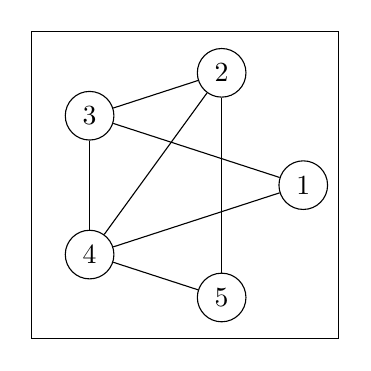
\begin{tikzpicture}
\tikzset{tinoeud/.style={draw, circle, minimum height=0.01cm}}
\clip (-2, -2) rectangle (2, 2);
\draw (-1.95, -1.95) rectangle (1.95, 1.95);
\node[tinoeud] (V1) at (0:1.5cm) {1};
\node[tinoeud] (V2) at (72:1.5cm) {2};
\node[tinoeud] (V3) at (144:1.5cm) {3};
\node[tinoeud] (V4) at (216:1.5cm) {4};
\node[tinoeud] (V5) at (288:1.5cm) {5};
\draw (V1) -- (V3);
\draw (V1) -- (V4);
\draw (V2) -- (V3);
\draw (V2) -- (V4);
\draw (V2) -- (V5);
\draw (V3) -- (V4);
\draw (V4) -- (V5);
\end{tikzpicture}
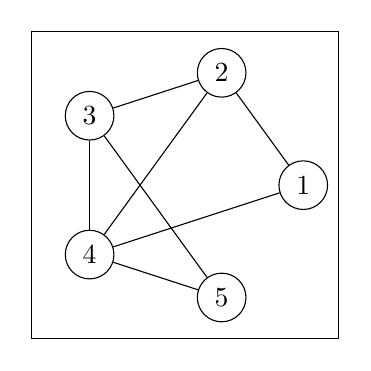
\begin{tikzpicture}
\tikzset{tinoeud/.style={draw, circle, minimum height=0.01cm}}
\clip (-2, -2) rectangle (2, 2);
\draw (-1.95, -1.95) rectangle (1.95, 1.95);
\node[tinoeud] (V1) at (0:1.5cm) {1};
\node[tinoeud] (V2) at (72:1.5cm) {2};
\node[tinoeud] (V3) at (144:1.5cm) {3};
\node[tinoeud] (V4) at (216:1.5cm) {4};
\node[tinoeud] (V5) at (288:1.5cm) {5};
\draw (V1) -- (V2);
\draw (V1) -- (V4);
\draw (V2) -- (V3);
\draw (V2) -- (V4);
\draw (V3) -- (V4);
\draw (V3) -- (V5);
\draw (V4) -- (V5);
\end{tikzpicture}
\newpage
classe de la partition grosse
\\
\begin{tabular}{c c c c c c}
\toprule 
Noeuds & Requête & Noeuds & Requête & Noeuds & Requête \\
\midrule 
1, 2, 3, 4 & 2.0 & 1, 2, 3, 5 & 3.0 & 1, 2, 4, 5 & 4.0 \\
1, 3, 4, 5 & 3.0 & 2, 3, 4, 5 & 3.0 \\
\bottomrule 
\end{tabular}
\\
\begin{center}
classe de la partition fine
\\
\begin{tabular}{c c c c c c}
\toprule 
Noeuds & Requête & Noeuds & Requête & Noeuds & Requête \\
\midrule 
1, 2, 3, 4 & 4 & 1, 2, 3, 5 & 10 & 1, 2, 4, 5 & 8 \\
1, 3, 4, 5 & 11 & 2, 3, 4, 5 & 11 \\
\bottomrule 
\end{tabular}
\end{center}
\\
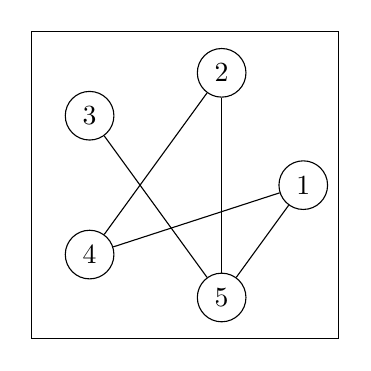
\begin{tikzpicture}
\tikzset{tinoeud/.style={draw, circle, minimum height=0.01cm}}
\clip (-2, -2) rectangle (2, 2);
\draw (-1.95, -1.95) rectangle (1.95, 1.95);
\node[tinoeud] (V1) at (0:1.5cm) {1};
\node[tinoeud] (V2) at (72:1.5cm) {2};
\node[tinoeud] (V3) at (144:1.5cm) {3};
\node[tinoeud] (V4) at (216:1.5cm) {4};
\node[tinoeud] (V5) at (288:1.5cm) {5};
\draw (V1) -- (V4);
\draw (V1) -- (V5);
\draw (V2) -- (V4);
\draw (V2) -- (V5);
\draw (V3) -- (V5);
\end{tikzpicture}
\begin{center}
classe de la partition fine
\\
\begin{tabular}{c c c c c c}
\toprule 
Noeuds & Requête & Noeuds & Requête & Noeuds & Requête \\
\midrule 
1, 2, 3, 4 & 7 & 1, 2, 3, 5 & 11 & 1, 2, 4, 5 & 5 \\
1, 3, 4, 5 & 9 & 2, 3, 4, 5 & 11 \\
\bottomrule 
\end{tabular}
\end{center}
\\
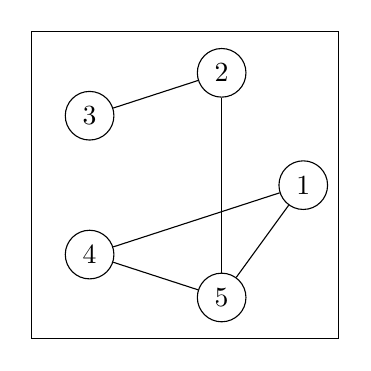
\begin{tikzpicture}
\tikzset{tinoeud/.style={draw, circle, minimum height=0.01cm}}
\clip (-2, -2) rectangle (2, 2);
\draw (-1.95, -1.95) rectangle (1.95, 1.95);
\node[tinoeud] (V1) at (0:1.5cm) {1};
\node[tinoeud] (V2) at (72:1.5cm) {2};
\node[tinoeud] (V3) at (144:1.5cm) {3};
\node[tinoeud] (V4) at (216:1.5cm) {4};
\node[tinoeud] (V5) at (288:1.5cm) {5};
\draw (V1) -- (V4);
\draw (V1) -- (V5);
\draw (V2) -- (V3);
\draw (V2) -- (V5);
\draw (V4) -- (V5);
\end{tikzpicture}
\newpage
\begin{center}
classe de la partition fine
\\
\begin{tabular}{c c c c c c}
\toprule 
Noeuds & Requête & Noeuds & Requête & Noeuds & Requête \\
\midrule 
1, 2, 3, 4 & 7 & 1, 2, 3, 5 & 11 & 1, 2, 4, 5 & 5 \\
1, 3, 4, 5 & 11 & 2, 3, 4, 5 & 9 \\
\bottomrule 
\end{tabular}
\end{center}
\\
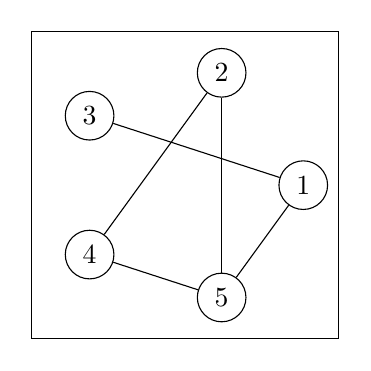
\begin{tikzpicture}
\tikzset{tinoeud/.style={draw, circle, minimum height=0.01cm}}
\clip (-2, -2) rectangle (2, 2);
\draw (-1.95, -1.95) rectangle (1.95, 1.95);
\node[tinoeud] (V1) at (0:1.5cm) {1};
\node[tinoeud] (V2) at (72:1.5cm) {2};
\node[tinoeud] (V3) at (144:1.5cm) {3};
\node[tinoeud] (V4) at (216:1.5cm) {4};
\node[tinoeud] (V5) at (288:1.5cm) {5};
\draw (V1) -- (V3);
\draw (V1) -- (V5);
\draw (V2) -- (V4);
\draw (V2) -- (V5);
\draw (V4) -- (V5);
\end{tikzpicture}
\begin{center}
classe de la partition fine
\\
\begin{tabular}{c c c c c c}
\toprule 
Noeuds & Requête & Noeuds & Requête & Noeuds & Requête \\
\midrule 
1, 2, 3, 4 & 7 & 1, 2, 3, 5 & 9 & 1, 2, 4, 5 & 5 \\
1, 3, 4, 5 & 11 & 2, 3, 4, 5 & 11 \\
\bottomrule 
\end{tabular}
\end{center}
\\
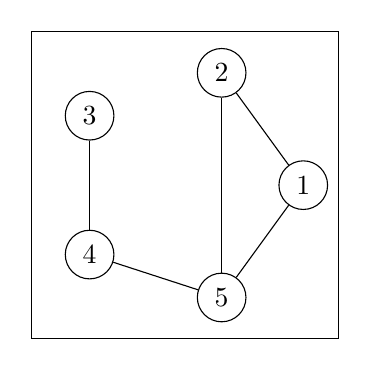
\begin{tikzpicture}
\tikzset{tinoeud/.style={draw, circle, minimum height=0.01cm}}
\clip (-2, -2) rectangle (2, 2);
\draw (-1.95, -1.95) rectangle (1.95, 1.95);
\node[tinoeud] (V1) at (0:1.5cm) {1};
\node[tinoeud] (V2) at (72:1.5cm) {2};
\node[tinoeud] (V3) at (144:1.5cm) {3};
\node[tinoeud] (V4) at (216:1.5cm) {4};
\node[tinoeud] (V5) at (288:1.5cm) {5};
\draw (V1) -- (V2);
\draw (V1) -- (V5);
\draw (V2) -- (V5);
\draw (V3) -- (V4);
\draw (V4) -- (V5);
\end{tikzpicture}
\newpage
\begin{center}
classe de la partition fine
\\
\begin{tabular}{c c c c c c}
\toprule 
Noeuds & Requête & Noeuds & Requête & Noeuds & Requête \\
\midrule 
1, 2, 3, 4 & 4 & 1, 2, 3, 5 & 11 & 1, 2, 4, 5 & 8 \\
1, 3, 4, 5 & 10 & 2, 3, 4, 5 & 11 \\
\bottomrule 
\end{tabular}
\end{center}
\\
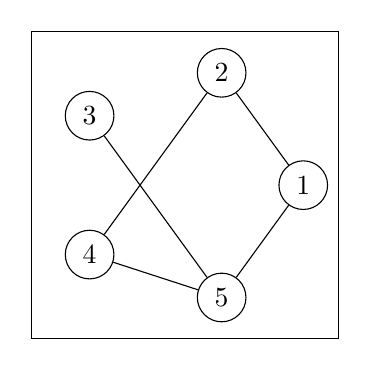
\begin{tikzpicture}
\tikzset{tinoeud/.style={draw, circle, minimum height=0.01cm}}
\clip (-2, -2) rectangle (2, 2);
\draw (-1.95, -1.95) rectangle (1.95, 1.95);
\node[tinoeud] (V1) at (0:1.5cm) {1};
\node[tinoeud] (V2) at (72:1.5cm) {2};
\node[tinoeud] (V3) at (144:1.5cm) {3};
\node[tinoeud] (V4) at (216:1.5cm) {4};
\node[tinoeud] (V5) at (288:1.5cm) {5};
\draw (V1) -- (V2);
\draw (V1) -- (V5);
\draw (V2) -- (V4);
\draw (V3) -- (V5);
\draw (V4) -- (V5);
\end{tikzpicture}
\begin{center}
classe de la partition fine
\\
\begin{tabular}{c c c c c c}
\toprule 
Noeuds & Requête & Noeuds & Requête & Noeuds & Requête \\
\midrule 
1, 2, 3, 4 & 4 & 1, 2, 3, 5 & 11 & 1, 2, 4, 5 & 8 \\
1, 3, 4, 5 & 11 & 2, 3, 4, 5 & 10 \\
\bottomrule 
\end{tabular}
\end{center}
\\
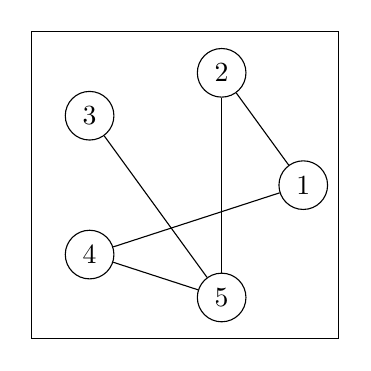
\begin{tikzpicture}
\tikzset{tinoeud/.style={draw, circle, minimum height=0.01cm}}
\clip (-2, -2) rectangle (2, 2);
\draw (-1.95, -1.95) rectangle (1.95, 1.95);
\node[tinoeud] (V1) at (0:1.5cm) {1};
\node[tinoeud] (V2) at (72:1.5cm) {2};
\node[tinoeud] (V3) at (144:1.5cm) {3};
\node[tinoeud] (V4) at (216:1.5cm) {4};
\node[tinoeud] (V5) at (288:1.5cm) {5};
\draw (V1) -- (V2);
\draw (V1) -- (V4);
\draw (V2) -- (V5);
\draw (V3) -- (V5);
\draw (V4) -- (V5);
\end{tikzpicture}
\newpage
\newpage
classe de la partition grosse
\\
\begin{tabular}{c c c c c c}
\toprule 
Noeuds & Requête & Noeuds & Requête & Noeuds & Requête \\
\midrule 
1, 2, 3, 4 & 3.0 & 1, 2, 3, 5 & 4.0 & 1, 2, 4, 5 & 3.0 \\
1, 3, 4, 5 & 3.0 & 2, 3, 4, 5 & 2.0 \\
\bottomrule 
\end{tabular}
\\
\begin{center}
classe de la partition fine
\\
\begin{tabular}{c c c c c c}
\toprule 
Noeuds & Requête & Noeuds & Requête & Noeuds & Requête \\
\midrule 
1, 2, 3, 4 & 11 & 1, 2, 3, 5 & 8 & 1, 2, 4, 5 & 11 \\
1, 3, 4, 5 & 10 & 2, 3, 4, 5 & 4 \\
\bottomrule 
\end{tabular}
\end{center}
\\
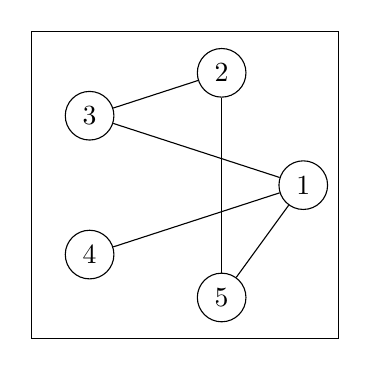
\begin{tikzpicture}
\tikzset{tinoeud/.style={draw, circle, minimum height=0.01cm}}
\clip (-2, -2) rectangle (2, 2);
\draw (-1.95, -1.95) rectangle (1.95, 1.95);
\node[tinoeud] (V1) at (0:1.5cm) {1};
\node[tinoeud] (V2) at (72:1.5cm) {2};
\node[tinoeud] (V3) at (144:1.5cm) {3};
\node[tinoeud] (V4) at (216:1.5cm) {4};
\node[tinoeud] (V5) at (288:1.5cm) {5};
\draw (V1) -- (V3);
\draw (V1) -- (V4);
\draw (V1) -- (V5);
\draw (V2) -- (V3);
\draw (V2) -- (V5);
\end{tikzpicture}
\begin{center}
classe de la partition fine
\\
\begin{tabular}{c c c c c c}
\toprule 
Noeuds & Requête & Noeuds & Requête & Noeuds & Requête \\
\midrule 
1, 2, 3, 4 & 11 & 1, 2, 3, 5 & 5 & 1, 2, 4, 5 & 9 \\
1, 3, 4, 5 & 11 & 2, 3, 4, 5 & 7 \\
\bottomrule 
\end{tabular}
\end{center}
\\
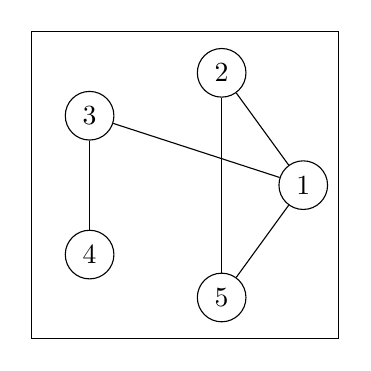
\begin{tikzpicture}
\tikzset{tinoeud/.style={draw, circle, minimum height=0.01cm}}
\clip (-2, -2) rectangle (2, 2);
\draw (-1.95, -1.95) rectangle (1.95, 1.95);
\node[tinoeud] (V1) at (0:1.5cm) {1};
\node[tinoeud] (V2) at (72:1.5cm) {2};
\node[tinoeud] (V3) at (144:1.5cm) {3};
\node[tinoeud] (V4) at (216:1.5cm) {4};
\node[tinoeud] (V5) at (288:1.5cm) {5};
\draw (V1) -- (V2);
\draw (V1) -- (V3);
\draw (V1) -- (V5);
\draw (V2) -- (V5);
\draw (V3) -- (V4);
\end{tikzpicture}
\newpage
\begin{center}
classe de la partition fine
\\
\begin{tabular}{c c c c c c}
\toprule 
Noeuds & Requête & Noeuds & Requête & Noeuds & Requête \\
\midrule 
1, 2, 3, 4 & 11 & 1, 2, 3, 5 & 8 & 1, 2, 4, 5 & 10 \\
1, 3, 4, 5 & 11 & 2, 3, 4, 5 & 4 \\
\bottomrule 
\end{tabular}
\end{center}
\\
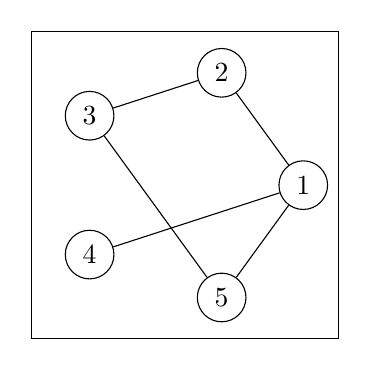
\begin{tikzpicture}
\tikzset{tinoeud/.style={draw, circle, minimum height=0.01cm}}
\clip (-2, -2) rectangle (2, 2);
\draw (-1.95, -1.95) rectangle (1.95, 1.95);
\node[tinoeud] (V1) at (0:1.5cm) {1};
\node[tinoeud] (V2) at (72:1.5cm) {2};
\node[tinoeud] (V3) at (144:1.5cm) {3};
\node[tinoeud] (V4) at (216:1.5cm) {4};
\node[tinoeud] (V5) at (288:1.5cm) {5};
\draw (V1) -- (V2);
\draw (V1) -- (V4);
\draw (V1) -- (V5);
\draw (V2) -- (V3);
\draw (V3) -- (V5);
\end{tikzpicture}
\begin{center}
classe de la partition fine
\\
\begin{tabular}{c c c c c c}
\toprule 
Noeuds & Requête & Noeuds & Requête & Noeuds & Requête \\
\midrule 
1, 2, 3, 4 & 11 & 1, 2, 3, 5 & 5 & 1, 2, 4, 5 & 11 \\
1, 3, 4, 5 & 9 & 2, 3, 4, 5 & 7 \\
\bottomrule 
\end{tabular}
\end{center}
\\
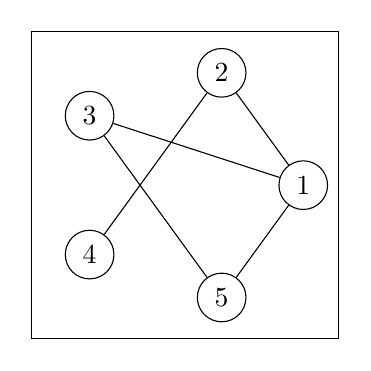
\begin{tikzpicture}
\tikzset{tinoeud/.style={draw, circle, minimum height=0.01cm}}
\clip (-2, -2) rectangle (2, 2);
\draw (-1.95, -1.95) rectangle (1.95, 1.95);
\node[tinoeud] (V1) at (0:1.5cm) {1};
\node[tinoeud] (V2) at (72:1.5cm) {2};
\node[tinoeud] (V3) at (144:1.5cm) {3};
\node[tinoeud] (V4) at (216:1.5cm) {4};
\node[tinoeud] (V5) at (288:1.5cm) {5};
\draw (V1) -- (V2);
\draw (V1) -- (V3);
\draw (V1) -- (V5);
\draw (V2) -- (V4);
\draw (V3) -- (V5);
\end{tikzpicture}
\newpage
\begin{center}
classe de la partition fine
\\
\begin{tabular}{c c c c c c}
\toprule 
Noeuds & Requête & Noeuds & Requête & Noeuds & Requête \\
\midrule 
1, 2, 3, 4 & 10 & 1, 2, 3, 5 & 8 & 1, 2, 4, 5 & 11 \\
1, 3, 4, 5 & 11 & 2, 3, 4, 5 & 4 \\
\bottomrule 
\end{tabular}
\end{center}
\\
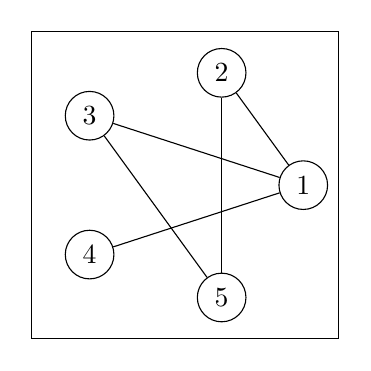
\begin{tikzpicture}
\tikzset{tinoeud/.style={draw, circle, minimum height=0.01cm}}
\clip (-2, -2) rectangle (2, 2);
\draw (-1.95, -1.95) rectangle (1.95, 1.95);
\node[tinoeud] (V1) at (0:1.5cm) {1};
\node[tinoeud] (V2) at (72:1.5cm) {2};
\node[tinoeud] (V3) at (144:1.5cm) {3};
\node[tinoeud] (V4) at (216:1.5cm) {4};
\node[tinoeud] (V5) at (288:1.5cm) {5};
\draw (V1) -- (V2);
\draw (V1) -- (V3);
\draw (V1) -- (V4);
\draw (V2) -- (V5);
\draw (V3) -- (V5);
\end{tikzpicture}
\begin{center}
classe de la partition fine
\\
\begin{tabular}{c c c c c c}
\toprule 
Noeuds & Requête & Noeuds & Requête & Noeuds & Requête \\
\midrule 
1, 2, 3, 4 & 9 & 1, 2, 3, 5 & 5 & 1, 2, 4, 5 & 11 \\
1, 3, 4, 5 & 11 & 2, 3, 4, 5 & 7 \\
\bottomrule 
\end{tabular}
\end{center}
\\
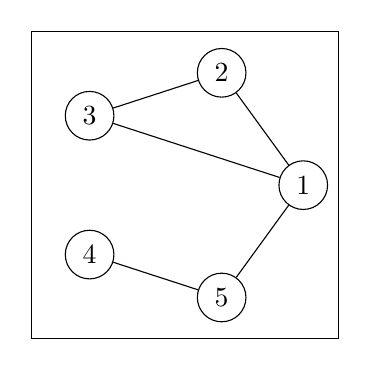
\begin{tikzpicture}
\tikzset{tinoeud/.style={draw, circle, minimum height=0.01cm}}
\clip (-2, -2) rectangle (2, 2);
\draw (-1.95, -1.95) rectangle (1.95, 1.95);
\node[tinoeud] (V1) at (0:1.5cm) {1};
\node[tinoeud] (V2) at (72:1.5cm) {2};
\node[tinoeud] (V3) at (144:1.5cm) {3};
\node[tinoeud] (V4) at (216:1.5cm) {4};
\node[tinoeud] (V5) at (288:1.5cm) {5};
\draw (V1) -- (V2);
\draw (V1) -- (V3);
\draw (V1) -- (V5);
\draw (V2) -- (V3);
\draw (V4) -- (V5);
\end{tikzpicture}
\newpage
\newpage
classe de la partition grosse
\\
\begin{tabular}{c c c c c c}
\toprule 
Noeuds & Requête & Noeuds & Requête & Noeuds & Requête \\
\midrule 
1, 2, 3, 4 & 3.0 & 1, 2, 3, 5 & 3.0 & 1, 2, 4, 5 & 2.0 \\
1, 3, 4, 5 & 3.0 & 2, 3, 4, 5 & 4.0 \\
\bottomrule 
\end{tabular}
\\
\begin{center}
classe de la partition fine
\\
\begin{tabular}{c c c c c c}
\toprule 
Noeuds & Requête & Noeuds & Requête & Noeuds & Requête \\
\midrule 
1, 2, 3, 4 & 9 & 1, 2, 3, 5 & 11 & 1, 2, 4, 5 & 7 \\
1, 3, 4, 5 & 11 & 2, 3, 4, 5 & 5 \\
\bottomrule 
\end{tabular}
\end{center}
\\
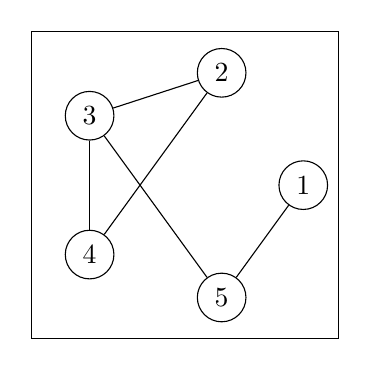
\begin{tikzpicture}
\tikzset{tinoeud/.style={draw, circle, minimum height=0.01cm}}
\clip (-2, -2) rectangle (2, 2);
\draw (-1.95, -1.95) rectangle (1.95, 1.95);
\node[tinoeud] (V1) at (0:1.5cm) {1};
\node[tinoeud] (V2) at (72:1.5cm) {2};
\node[tinoeud] (V3) at (144:1.5cm) {3};
\node[tinoeud] (V4) at (216:1.5cm) {4};
\node[tinoeud] (V5) at (288:1.5cm) {5};
\draw (V1) -- (V5);
\draw (V2) -- (V3);
\draw (V2) -- (V4);
\draw (V3) -- (V4);
\draw (V3) -- (V5);
\end{tikzpicture}
\begin{center}
classe de la partition fine
\\
\begin{tabular}{c c c c c c}
\toprule 
Noeuds & Requête & Noeuds & Requête & Noeuds & Requête \\
\midrule 
1, 2, 3, 4 & 11 & 1, 2, 3, 5 & 9 & 1, 2, 4, 5 & 7 \\
1, 3, 4, 5 & 11 & 2, 3, 4, 5 & 5 \\
\bottomrule 
\end{tabular}
\end{center}
\\
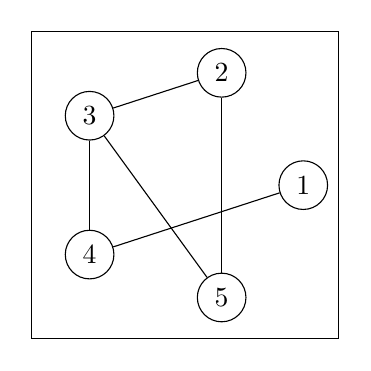
\begin{tikzpicture}
\tikzset{tinoeud/.style={draw, circle, minimum height=0.01cm}}
\clip (-2, -2) rectangle (2, 2);
\draw (-1.95, -1.95) rectangle (1.95, 1.95);
\node[tinoeud] (V1) at (0:1.5cm) {1};
\node[tinoeud] (V2) at (72:1.5cm) {2};
\node[tinoeud] (V3) at (144:1.5cm) {3};
\node[tinoeud] (V4) at (216:1.5cm) {4};
\node[tinoeud] (V5) at (288:1.5cm) {5};
\draw (V1) -- (V4);
\draw (V2) -- (V3);
\draw (V2) -- (V5);
\draw (V3) -- (V4);
\draw (V3) -- (V5);
\end{tikzpicture}
\newpage
\begin{center}
classe de la partition fine
\\
\begin{tabular}{c c c c c c}
\toprule 
Noeuds & Requête & Noeuds & Requête & Noeuds & Requête \\
\midrule 
1, 2, 3, 4 & 11 & 1, 2, 3, 5 & 11 & 1, 2, 4, 5 & 4 \\
1, 3, 4, 5 & 10 & 2, 3, 4, 5 & 8 \\
\bottomrule 
\end{tabular}
\end{center}
\\
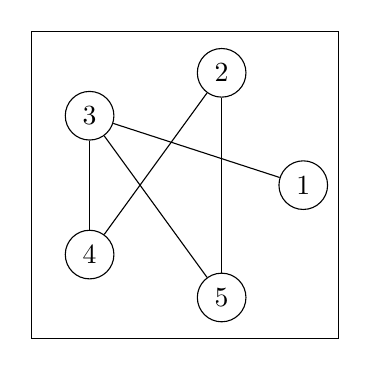
\begin{tikzpicture}
\tikzset{tinoeud/.style={draw, circle, minimum height=0.01cm}}
\clip (-2, -2) rectangle (2, 2);
\draw (-1.95, -1.95) rectangle (1.95, 1.95);
\node[tinoeud] (V1) at (0:1.5cm) {1};
\node[tinoeud] (V2) at (72:1.5cm) {2};
\node[tinoeud] (V3) at (144:1.5cm) {3};
\node[tinoeud] (V4) at (216:1.5cm) {4};
\node[tinoeud] (V5) at (288:1.5cm) {5};
\draw (V1) -- (V3);
\draw (V2) -- (V4);
\draw (V2) -- (V5);
\draw (V3) -- (V4);
\draw (V3) -- (V5);
\end{tikzpicture}
\begin{center}
classe de la partition fine
\\
\begin{tabular}{c c c c c c}
\toprule 
Noeuds & Requête & Noeuds & Requête & Noeuds & Requête \\
\midrule 
1, 2, 3, 4 & 10 & 1, 2, 3, 5 & 11 & 1, 2, 4, 5 & 4 \\
1, 3, 4, 5 & 11 & 2, 3, 4, 5 & 8 \\
\bottomrule 
\end{tabular}
\end{center}
\\
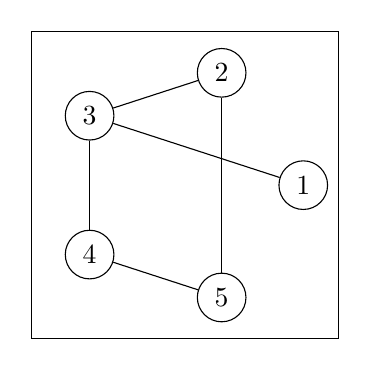
\begin{tikzpicture}
\tikzset{tinoeud/.style={draw, circle, minimum height=0.01cm}}
\clip (-2, -2) rectangle (2, 2);
\draw (-1.95, -1.95) rectangle (1.95, 1.95);
\node[tinoeud] (V1) at (0:1.5cm) {1};
\node[tinoeud] (V2) at (72:1.5cm) {2};
\node[tinoeud] (V3) at (144:1.5cm) {3};
\node[tinoeud] (V4) at (216:1.5cm) {4};
\node[tinoeud] (V5) at (288:1.5cm) {5};
\draw (V1) -- (V3);
\draw (V2) -- (V3);
\draw (V2) -- (V5);
\draw (V3) -- (V4);
\draw (V4) -- (V5);
\end{tikzpicture}
\newpage
\begin{center}
classe de la partition fine
\\
\begin{tabular}{c c c c c c}
\toprule 
Noeuds & Requête & Noeuds & Requête & Noeuds & Requête \\
\midrule 
1, 2, 3, 4 & 11 & 1, 2, 3, 5 & 10 & 1, 2, 4, 5 & 4 \\
1, 3, 4, 5 & 11 & 2, 3, 4, 5 & 8 \\
\bottomrule 
\end{tabular}
\end{center}
\\
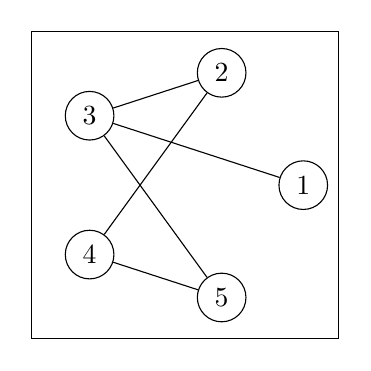
\begin{tikzpicture}
\tikzset{tinoeud/.style={draw, circle, minimum height=0.01cm}}
\clip (-2, -2) rectangle (2, 2);
\draw (-1.95, -1.95) rectangle (1.95, 1.95);
\node[tinoeud] (V1) at (0:1.5cm) {1};
\node[tinoeud] (V2) at (72:1.5cm) {2};
\node[tinoeud] (V3) at (144:1.5cm) {3};
\node[tinoeud] (V4) at (216:1.5cm) {4};
\node[tinoeud] (V5) at (288:1.5cm) {5};
\draw (V1) -- (V3);
\draw (V2) -- (V3);
\draw (V2) -- (V4);
\draw (V3) -- (V5);
\draw (V4) -- (V5);
\end{tikzpicture}
\begin{center}
classe de la partition fine
\\
\begin{tabular}{c c c c c c}
\toprule 
Noeuds & Requête & Noeuds & Requête & Noeuds & Requête \\
\midrule 
1, 2, 3, 4 & 11 & 1, 2, 3, 5 & 11 & 1, 2, 4, 5 & 7 \\
1, 3, 4, 5 & 9 & 2, 3, 4, 5 & 5 \\
\bottomrule 
\end{tabular}
\end{center}
\\
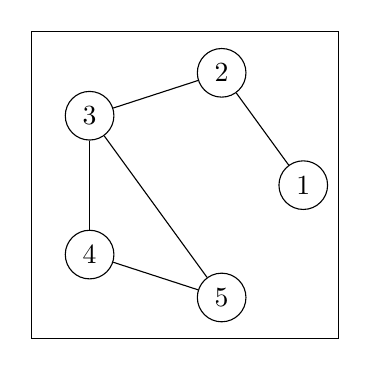
\begin{tikzpicture}
\tikzset{tinoeud/.style={draw, circle, minimum height=0.01cm}}
\clip (-2, -2) rectangle (2, 2);
\draw (-1.95, -1.95) rectangle (1.95, 1.95);
\node[tinoeud] (V1) at (0:1.5cm) {1};
\node[tinoeud] (V2) at (72:1.5cm) {2};
\node[tinoeud] (V3) at (144:1.5cm) {3};
\node[tinoeud] (V4) at (216:1.5cm) {4};
\node[tinoeud] (V5) at (288:1.5cm) {5};
\draw (V1) -- (V2);
\draw (V2) -- (V3);
\draw (V3) -- (V4);
\draw (V3) -- (V5);
\draw (V4) -- (V5);
\end{tikzpicture}
\newpage
\newpage
classe de la partition grosse
\\
\begin{tabular}{c c c c c c}
\toprule 
Noeuds & Requête & Noeuds & Requête & Noeuds & Requête \\
\midrule 
1, 2, 3, 4 & 2.0 & 1, 2, 3, 5 & 1.0 & 1, 2, 4, 5 & 3.0 \\
1, 3, 4, 5 & 3.0 & 2, 3, 4, 5 & 3.0 \\
\bottomrule 
\end{tabular}
\\
\begin{center}
classe de la partition fine
\\
\begin{tabular}{c c c c c c}
\toprule 
Noeuds & Requête & Noeuds & Requête & Noeuds & Requête \\
\midrule 
1, 2, 3, 4 & 4 & 1, 2, 3, 5 & 2 & 1, 2, 4, 5 & 11 \\
1, 3, 4, 5 & 11 & 2, 3, 4, 5 & 10 \\
\bottomrule 
\end{tabular}
\end{center}
\\
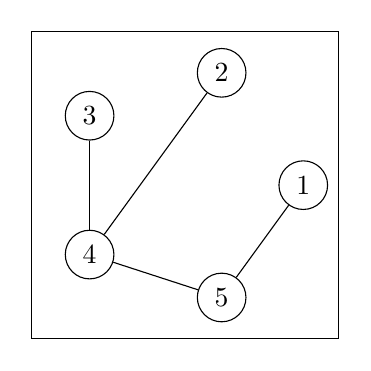
\begin{tikzpicture}
\tikzset{tinoeud/.style={draw, circle, minimum height=0.01cm}}
\clip (-2, -2) rectangle (2, 2);
\draw (-1.95, -1.95) rectangle (1.95, 1.95);
\node[tinoeud] (V1) at (0:1.5cm) {1};
\node[tinoeud] (V2) at (72:1.5cm) {2};
\node[tinoeud] (V3) at (144:1.5cm) {3};
\node[tinoeud] (V4) at (216:1.5cm) {4};
\node[tinoeud] (V5) at (288:1.5cm) {5};
\draw (V1) -- (V5);
\draw (V2) -- (V4);
\draw (V3) -- (V4);
\draw (V4) -- (V5);
\end{tikzpicture}
\begin{center}
classe de la partition fine
\\
\begin{tabular}{c c c c c c}
\toprule 
Noeuds & Requête & Noeuds & Requête & Noeuds & Requête \\
\midrule 
1, 2, 3, 4 & 4 & 1, 2, 3, 5 & 2 & 1, 2, 4, 5 & 11 \\
1, 3, 4, 5 & 10 & 2, 3, 4, 5 & 11 \\
\bottomrule 
\end{tabular}
\end{center}
\\
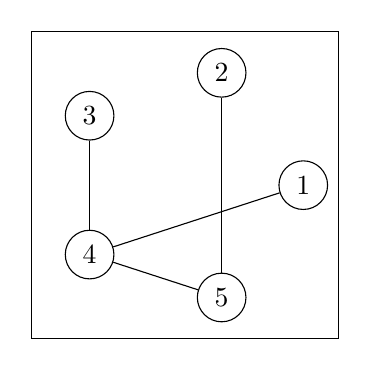
\begin{tikzpicture}
\tikzset{tinoeud/.style={draw, circle, minimum height=0.01cm}}
\clip (-2, -2) rectangle (2, 2);
\draw (-1.95, -1.95) rectangle (1.95, 1.95);
\node[tinoeud] (V1) at (0:1.5cm) {1};
\node[tinoeud] (V2) at (72:1.5cm) {2};
\node[tinoeud] (V3) at (144:1.5cm) {3};
\node[tinoeud] (V4) at (216:1.5cm) {4};
\node[tinoeud] (V5) at (288:1.5cm) {5};
\draw (V1) -- (V4);
\draw (V2) -- (V5);
\draw (V3) -- (V4);
\draw (V4) -- (V5);
\end{tikzpicture}
\newpage
\begin{center}
classe de la partition fine
\\
\begin{tabular}{c c c c c c}
\toprule 
Noeuds & Requête & Noeuds & Requête & Noeuds & Requête \\
\midrule 
1, 2, 3, 4 & 4 & 1, 2, 3, 5 & 2 & 1, 2, 4, 5 & 10 \\
1, 3, 4, 5 & 11 & 2, 3, 4, 5 & 11 \\
\bottomrule 
\end{tabular}
\end{center}
\\
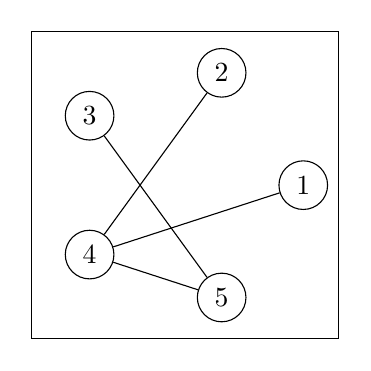
\begin{tikzpicture}
\tikzset{tinoeud/.style={draw, circle, minimum height=0.01cm}}
\clip (-2, -2) rectangle (2, 2);
\draw (-1.95, -1.95) rectangle (1.95, 1.95);
\node[tinoeud] (V1) at (0:1.5cm) {1};
\node[tinoeud] (V2) at (72:1.5cm) {2};
\node[tinoeud] (V3) at (144:1.5cm) {3};
\node[tinoeud] (V4) at (216:1.5cm) {4};
\node[tinoeud] (V5) at (288:1.5cm) {5};
\draw (V1) -- (V4);
\draw (V2) -- (V4);
\draw (V3) -- (V5);
\draw (V4) -- (V5);
\end{tikzpicture}
\newpage
classe de la partition grosse
\\
\begin{tabular}{c c c c c c}
\toprule 
Noeuds & Requête & Noeuds & Requête & Noeuds & Requête \\
\midrule 
1, 2, 3, 4 & 3.0 & 1, 2, 3, 5 & 2.0 & 1, 2, 4, 5 & 3.0 \\
1, 3, 4, 5 & 2.0 & 2, 3, 4, 5 & 2.0 \\
\bottomrule 
\end{tabular}
\\
\begin{center}
classe de la partition fine
\\
\begin{tabular}{c c c c c c}
\toprule 
Noeuds & Requête & Noeuds & Requête & Noeuds & Requête \\
\midrule 
1, 2, 3, 4 & 11 & 1, 2, 3, 5 & 7 & 1, 2, 4, 5 & 11 \\
1, 3, 4, 5 & 4 & 2, 3, 4, 5 & 4 \\
\bottomrule 
\end{tabular}
\end{center}
\\
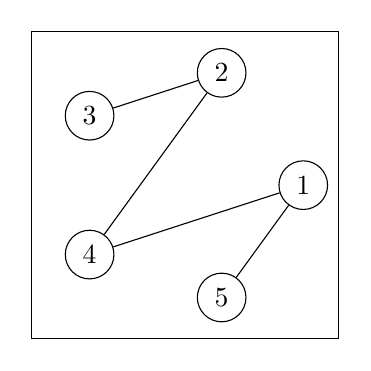
\begin{tikzpicture}
\tikzset{tinoeud/.style={draw, circle, minimum height=0.01cm}}
\clip (-2, -2) rectangle (2, 2);
\draw (-1.95, -1.95) rectangle (1.95, 1.95);
\node[tinoeud] (V1) at (0:1.5cm) {1};
\node[tinoeud] (V2) at (72:1.5cm) {2};
\node[tinoeud] (V3) at (144:1.5cm) {3};
\node[tinoeud] (V4) at (216:1.5cm) {4};
\node[tinoeud] (V5) at (288:1.5cm) {5};
\draw (V1) -- (V4);
\draw (V1) -- (V5);
\draw (V2) -- (V3);
\draw (V2) -- (V4);
\end{tikzpicture}
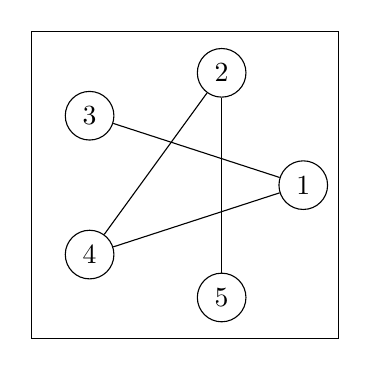
\begin{tikzpicture}
\tikzset{tinoeud/.style={draw, circle, minimum height=0.01cm}}
\clip (-2, -2) rectangle (2, 2);
\draw (-1.95, -1.95) rectangle (1.95, 1.95);
\node[tinoeud] (V1) at (0:1.5cm) {1};
\node[tinoeud] (V2) at (72:1.5cm) {2};
\node[tinoeud] (V3) at (144:1.5cm) {3};
\node[tinoeud] (V4) at (216:1.5cm) {4};
\node[tinoeud] (V5) at (288:1.5cm) {5};
\draw (V1) -- (V3);
\draw (V1) -- (V4);
\draw (V2) -- (V4);
\draw (V2) -- (V5);
\end{tikzpicture}
\begin{center}
classe de la partition fine
\\
\begin{tabular}{c c c c c c}
\toprule 
Noeuds & Requête & Noeuds & Requête & Noeuds & Requête \\
\midrule 
1, 2, 3, 4 & 11 & 1, 2, 3, 5 & 4 & 1, 2, 4, 5 & 11 \\
1, 3, 4, 5 & 7 & 2, 3, 4, 5 & 4 \\
\bottomrule 
\end{tabular}
\end{center}
\\
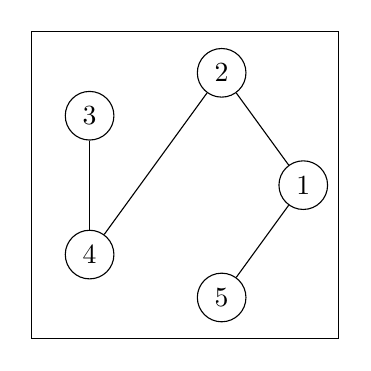
\begin{tikzpicture}
\tikzset{tinoeud/.style={draw, circle, minimum height=0.01cm}}
\clip (-2, -2) rectangle (2, 2);
\draw (-1.95, -1.95) rectangle (1.95, 1.95);
\node[tinoeud] (V1) at (0:1.5cm) {1};
\node[tinoeud] (V2) at (72:1.5cm) {2};
\node[tinoeud] (V3) at (144:1.5cm) {3};
\node[tinoeud] (V4) at (216:1.5cm) {4};
\node[tinoeud] (V5) at (288:1.5cm) {5};
\draw (V1) -- (V2);
\draw (V1) -- (V5);
\draw (V2) -- (V4);
\draw (V3) -- (V4);
\end{tikzpicture}
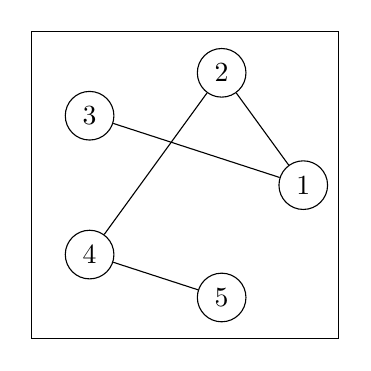
\begin{tikzpicture}
\tikzset{tinoeud/.style={draw, circle, minimum height=0.01cm}}
\clip (-2, -2) rectangle (2, 2);
\draw (-1.95, -1.95) rectangle (1.95, 1.95);
\node[tinoeud] (V1) at (0:1.5cm) {1};
\node[tinoeud] (V2) at (72:1.5cm) {2};
\node[tinoeud] (V3) at (144:1.5cm) {3};
\node[tinoeud] (V4) at (216:1.5cm) {4};
\node[tinoeud] (V5) at (288:1.5cm) {5};
\draw (V1) -- (V2);
\draw (V1) -- (V3);
\draw (V2) -- (V4);
\draw (V4) -- (V5);
\end{tikzpicture}
\newpage
\begin{center}
classe de la partition fine
\\
\begin{tabular}{c c c c c c}
\toprule 
Noeuds & Requête & Noeuds & Requête & Noeuds & Requête \\
\midrule 
1, 2, 3, 4 & 11 & 1, 2, 3, 5 & 4 & 1, 2, 4, 5 & 11 \\
1, 3, 4, 5 & 4 & 2, 3, 4, 5 & 7 \\
\bottomrule 
\end{tabular}
\end{center}
\\
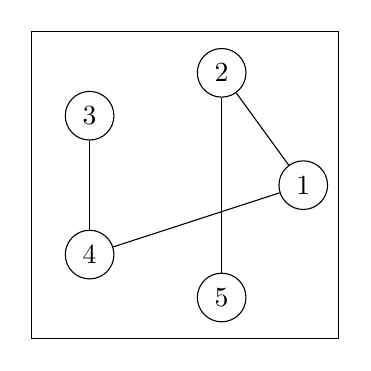
\begin{tikzpicture}
\tikzset{tinoeud/.style={draw, circle, minimum height=0.01cm}}
\clip (-2, -2) rectangle (2, 2);
\draw (-1.95, -1.95) rectangle (1.95, 1.95);
\node[tinoeud] (V1) at (0:1.5cm) {1};
\node[tinoeud] (V2) at (72:1.5cm) {2};
\node[tinoeud] (V3) at (144:1.5cm) {3};
\node[tinoeud] (V4) at (216:1.5cm) {4};
\node[tinoeud] (V5) at (288:1.5cm) {5};
\draw (V1) -- (V2);
\draw (V1) -- (V4);
\draw (V2) -- (V5);
\draw (V3) -- (V4);
\end{tikzpicture}
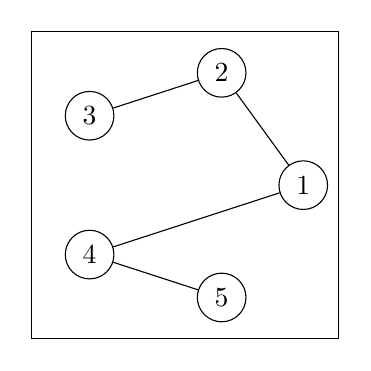
\begin{tikzpicture}
\tikzset{tinoeud/.style={draw, circle, minimum height=0.01cm}}
\clip (-2, -2) rectangle (2, 2);
\draw (-1.95, -1.95) rectangle (1.95, 1.95);
\node[tinoeud] (V1) at (0:1.5cm) {1};
\node[tinoeud] (V2) at (72:1.5cm) {2};
\node[tinoeud] (V3) at (144:1.5cm) {3};
\node[tinoeud] (V4) at (216:1.5cm) {4};
\node[tinoeud] (V5) at (288:1.5cm) {5};
\draw (V1) -- (V2);
\draw (V1) -- (V4);
\draw (V2) -- (V3);
\draw (V4) -- (V5);
\end{tikzpicture}
\begin{center}
classe de la partition fine
\\
\begin{tabular}{c c c c c c}
\toprule 
Noeuds & Requête & Noeuds & Requête & Noeuds & Requête \\
\midrule 
1, 2, 3, 4 & 9 & 1, 2, 3, 5 & 7 & 1, 2, 4, 5 & 9 \\
1, 3, 4, 5 & 7 & 2, 3, 4, 5 & 7 \\
\bottomrule 
\end{tabular}
\end{center}
\\
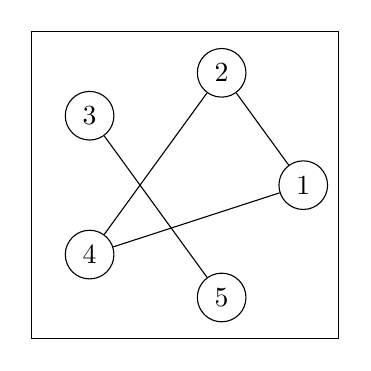
\begin{tikzpicture}
\tikzset{tinoeud/.style={draw, circle, minimum height=0.01cm}}
\clip (-2, -2) rectangle (2, 2);
\draw (-1.95, -1.95) rectangle (1.95, 1.95);
\node[tinoeud] (V1) at (0:1.5cm) {1};
\node[tinoeud] (V2) at (72:1.5cm) {2};
\node[tinoeud] (V3) at (144:1.5cm) {3};
\node[tinoeud] (V4) at (216:1.5cm) {4};
\node[tinoeud] (V5) at (288:1.5cm) {5};
\draw (V1) -- (V2);
\draw (V1) -- (V4);
\draw (V2) -- (V4);
\draw (V3) -- (V5);
\end{tikzpicture}
\newpage
\newpage
classe de la partition grosse
\\
\begin{tabular}{c c c c c c}
\toprule 
Noeuds & Requête & Noeuds & Requête & Noeuds & Requête \\
\midrule 
1, 2, 3, 4 & 4.0 & 1, 2, 3, 5 & 3.0 & 1, 2, 4, 5 & 5.0 \\
1, 3, 4, 5 & 5.0 & 2, 3, 4, 5 & 4.0 \\
\bottomrule 
\end{tabular}
\\
\begin{center}
classe de la partition fine
\\
\begin{tabular}{c c c c c c}
\toprule 
Noeuds & Requête & Noeuds & Requête & Noeuds & Requête \\
\midrule 
1, 2, 3, 4 & 5 & 1, 2, 3, 5 & 11 & 1, 2, 4, 5 & 3 \\
1, 3, 4, 5 & 3 & 2, 3, 4, 5 & 5 \\
\bottomrule 
\end{tabular}
\end{center}
\\
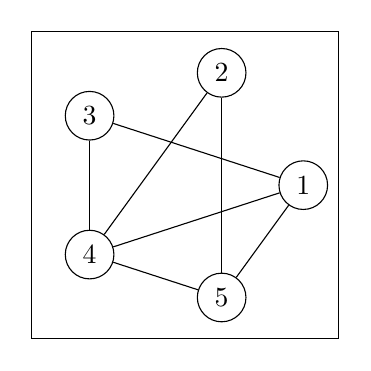
\begin{tikzpicture}
\tikzset{tinoeud/.style={draw, circle, minimum height=0.01cm}}
\clip (-2, -2) rectangle (2, 2);
\draw (-1.95, -1.95) rectangle (1.95, 1.95);
\node[tinoeud] (V1) at (0:1.5cm) {1};
\node[tinoeud] (V2) at (72:1.5cm) {2};
\node[tinoeud] (V3) at (144:1.5cm) {3};
\node[tinoeud] (V4) at (216:1.5cm) {4};
\node[tinoeud] (V5) at (288:1.5cm) {5};
\draw (V1) -- (V3);
\draw (V1) -- (V4);
\draw (V1) -- (V5);
\draw (V2) -- (V4);
\draw (V2) -- (V5);
\draw (V3) -- (V4);
\draw (V4) -- (V5);
\end{tikzpicture}
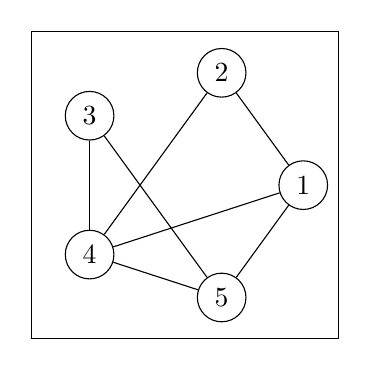
\begin{tikzpicture}
\tikzset{tinoeud/.style={draw, circle, minimum height=0.01cm}}
\clip (-2, -2) rectangle (2, 2);
\draw (-1.95, -1.95) rectangle (1.95, 1.95);
\node[tinoeud] (V1) at (0:1.5cm) {1};
\node[tinoeud] (V2) at (72:1.5cm) {2};
\node[tinoeud] (V3) at (144:1.5cm) {3};
\node[tinoeud] (V4) at (216:1.5cm) {4};
\node[tinoeud] (V5) at (288:1.5cm) {5};
\draw (V1) -- (V2);
\draw (V1) -- (V4);
\draw (V1) -- (V5);
\draw (V2) -- (V4);
\draw (V3) -- (V4);
\draw (V3) -- (V5);
\draw (V4) -- (V5);
\end{tikzpicture}
\newpage
classe de la partition grosse
\\
\begin{tabular}{c c c c c c}
\toprule 
Noeuds & Requête & Noeuds & Requête & Noeuds & Requête \\
\midrule 
1, 2, 3, 4 & 4.0 & 1, 2, 3, 5 & 4.0 & 1, 2, 4, 5 & 5.0 \\
1, 3, 4, 5 & 4.0 & 2, 3, 4, 5 & 4.0 \\
\bottomrule 
\end{tabular}
\\
\begin{center}
classe de la partition fine
\\
\begin{tabular}{c c c c c c}
\toprule 
Noeuds & Requête & Noeuds & Requête & Noeuds & Requête \\
\midrule 
1, 2, 3, 4 & 5 & 1, 2, 3, 5 & 5 & 1, 2, 4, 5 & 3 \\
1, 3, 4, 5 & 8 & 2, 3, 4, 5 & 8 \\
\bottomrule 
\end{tabular}
\end{center}
\\
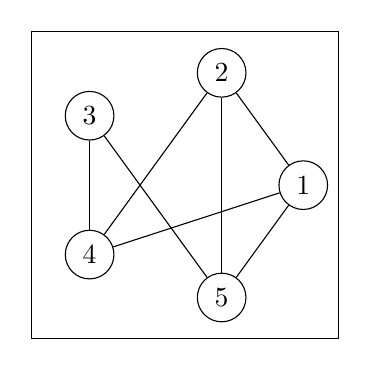
\begin{tikzpicture}
\tikzset{tinoeud/.style={draw, circle, minimum height=0.01cm}}
\clip (-2, -2) rectangle (2, 2);
\draw (-1.95, -1.95) rectangle (1.95, 1.95);
\node[tinoeud] (V1) at (0:1.5cm) {1};
\node[tinoeud] (V2) at (72:1.5cm) {2};
\node[tinoeud] (V3) at (144:1.5cm) {3};
\node[tinoeud] (V4) at (216:1.5cm) {4};
\node[tinoeud] (V5) at (288:1.5cm) {5};
\draw (V1) -- (V2);
\draw (V1) -- (V4);
\draw (V1) -- (V5);
\draw (V2) -- (V4);
\draw (V2) -- (V5);
\draw (V3) -- (V4);
\draw (V3) -- (V5);
\end{tikzpicture}
\begin{center}
classe de la partition fine
\\
\begin{tabular}{c c c c c c}
\toprule 
Noeuds & Requête & Noeuds & Requête & Noeuds & Requête \\
\midrule 
1, 2, 3, 4 & 8 & 1, 2, 3, 5 & 8 & 1, 2, 4, 5 & 3 \\
1, 3, 4, 5 & 5 & 2, 3, 4, 5 & 5 \\
\bottomrule 
\end{tabular}
\end{center}
\\
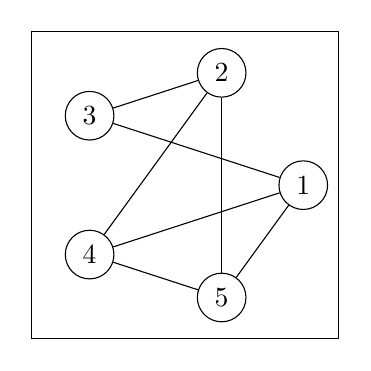
\begin{tikzpicture}
\tikzset{tinoeud/.style={draw, circle, minimum height=0.01cm}}
\clip (-2, -2) rectangle (2, 2);
\draw (-1.95, -1.95) rectangle (1.95, 1.95);
\node[tinoeud] (V1) at (0:1.5cm) {1};
\node[tinoeud] (V2) at (72:1.5cm) {2};
\node[tinoeud] (V3) at (144:1.5cm) {3};
\node[tinoeud] (V4) at (216:1.5cm) {4};
\node[tinoeud] (V5) at (288:1.5cm) {5};
\draw (V1) -- (V3);
\draw (V1) -- (V4);
\draw (V1) -- (V5);
\draw (V2) -- (V3);
\draw (V2) -- (V4);
\draw (V2) -- (V5);
\draw (V4) -- (V5);
\end{tikzpicture}
\newpage
\begin{center}
classe de la partition fine
\\
\begin{tabular}{c c c c c c}
\toprule 
Noeuds & Requête & Noeuds & Requête & Noeuds & Requête \\
\midrule 
1, 2, 3, 4 & 8 & 1, 2, 3, 5 & 5 & 1, 2, 4, 5 & 3 \\
1, 3, 4, 5 & 5 & 2, 3, 4, 5 & 8 \\
\bottomrule 
\end{tabular}
\end{center}
\\
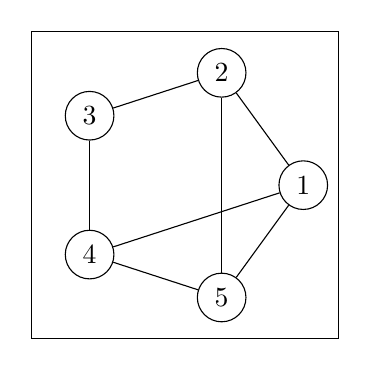
\begin{tikzpicture}
\tikzset{tinoeud/.style={draw, circle, minimum height=0.01cm}}
\clip (-2, -2) rectangle (2, 2);
\draw (-1.95, -1.95) rectangle (1.95, 1.95);
\node[tinoeud] (V1) at (0:1.5cm) {1};
\node[tinoeud] (V2) at (72:1.5cm) {2};
\node[tinoeud] (V3) at (144:1.5cm) {3};
\node[tinoeud] (V4) at (216:1.5cm) {4};
\node[tinoeud] (V5) at (288:1.5cm) {5};
\draw (V1) -- (V2);
\draw (V1) -- (V4);
\draw (V1) -- (V5);
\draw (V2) -- (V3);
\draw (V2) -- (V5);
\draw (V3) -- (V4);
\draw (V4) -- (V5);
\end{tikzpicture}
\begin{center}
classe de la partition fine
\\
\begin{tabular}{c c c c c c}
\toprule 
Noeuds & Requête & Noeuds & Requête & Noeuds & Requête \\
\midrule 
1, 2, 3, 4 & 8 & 1, 2, 3, 5 & 5 & 1, 2, 4, 5 & 3 \\
1, 3, 4, 5 & 8 & 2, 3, 4, 5 & 5 \\
\bottomrule 
\end{tabular}
\end{center}
\\
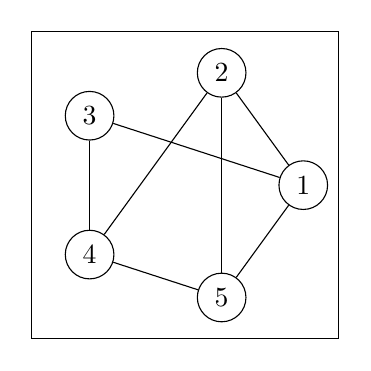
\begin{tikzpicture}
\tikzset{tinoeud/.style={draw, circle, minimum height=0.01cm}}
\clip (-2, -2) rectangle (2, 2);
\draw (-1.95, -1.95) rectangle (1.95, 1.95);
\node[tinoeud] (V1) at (0:1.5cm) {1};
\node[tinoeud] (V2) at (72:1.5cm) {2};
\node[tinoeud] (V3) at (144:1.5cm) {3};
\node[tinoeud] (V4) at (216:1.5cm) {4};
\node[tinoeud] (V5) at (288:1.5cm) {5};
\draw (V1) -- (V2);
\draw (V1) -- (V3);
\draw (V1) -- (V5);
\draw (V2) -- (V4);
\draw (V2) -- (V5);
\draw (V3) -- (V4);
\draw (V4) -- (V5);
\end{tikzpicture}
\newpage
\begin{center}
classe de la partition fine
\\
\begin{tabular}{c c c c c c}
\toprule 
Noeuds & Requête & Noeuds & Requête & Noeuds & Requête \\
\midrule 
1, 2, 3, 4 & 5 & 1, 2, 3, 5 & 8 & 1, 2, 4, 5 & 3 \\
1, 3, 4, 5 & 5 & 2, 3, 4, 5 & 8 \\
\bottomrule 
\end{tabular}
\end{center}
\\
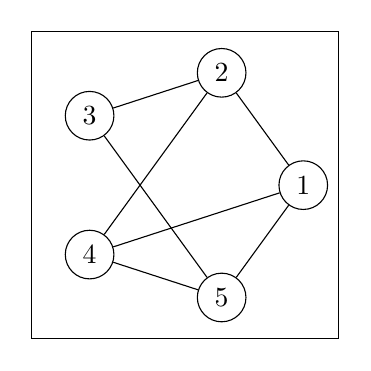
\begin{tikzpicture}
\tikzset{tinoeud/.style={draw, circle, minimum height=0.01cm}}
\clip (-2, -2) rectangle (2, 2);
\draw (-1.95, -1.95) rectangle (1.95, 1.95);
\node[tinoeud] (V1) at (0:1.5cm) {1};
\node[tinoeud] (V2) at (72:1.5cm) {2};
\node[tinoeud] (V3) at (144:1.5cm) {3};
\node[tinoeud] (V4) at (216:1.5cm) {4};
\node[tinoeud] (V5) at (288:1.5cm) {5};
\draw (V1) -- (V2);
\draw (V1) -- (V4);
\draw (V1) -- (V5);
\draw (V2) -- (V3);
\draw (V2) -- (V4);
\draw (V3) -- (V5);
\draw (V4) -- (V5);
\end{tikzpicture}
\begin{center}
classe de la partition fine
\\
\begin{tabular}{c c c c c c}
\toprule 
Noeuds & Requête & Noeuds & Requête & Noeuds & Requête \\
\midrule 
1, 2, 3, 4 & 5 & 1, 2, 3, 5 & 8 & 1, 2, 4, 5 & 3 \\
1, 3, 4, 5 & 8 & 2, 3, 4, 5 & 5 \\
\bottomrule 
\end{tabular}
\end{center}
\\
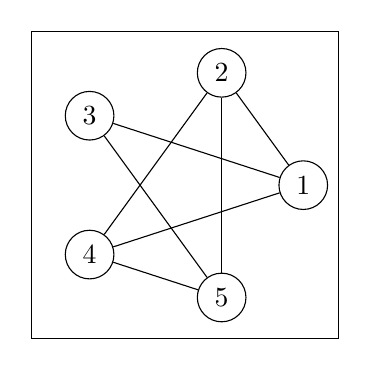
\begin{tikzpicture}
\tikzset{tinoeud/.style={draw, circle, minimum height=0.01cm}}
\clip (-2, -2) rectangle (2, 2);
\draw (-1.95, -1.95) rectangle (1.95, 1.95);
\node[tinoeud] (V1) at (0:1.5cm) {1};
\node[tinoeud] (V2) at (72:1.5cm) {2};
\node[tinoeud] (V3) at (144:1.5cm) {3};
\node[tinoeud] (V4) at (216:1.5cm) {4};
\node[tinoeud] (V5) at (288:1.5cm) {5};
\draw (V1) -- (V2);
\draw (V1) -- (V3);
\draw (V1) -- (V4);
\draw (V2) -- (V4);
\draw (V2) -- (V5);
\draw (V3) -- (V5);
\draw (V4) -- (V5);
\end{tikzpicture}
\newpage
\newpage
classe de la partition grosse
\\
\begin{tabular}{c c c c c c}
\toprule 
Noeuds & Requête & Noeuds & Requête & Noeuds & Requête \\
\midrule 
1, 2, 3, 4 & 1.0 & 1, 2, 3, 5 & 1.0 & 1, 2, 4, 5 & 2.0 \\
1, 3, 4, 5 & 1.0 & 2, 3, 4, 5 & 1.0 \\
\bottomrule 
\end{tabular}
\\
\begin{center}
classe de la partition fine
\\
\begin{tabular}{c c c c c c}
\toprule 
Noeuds & Requête & Noeuds & Requête & Noeuds & Requête \\
\midrule 
1, 2, 3, 4 & 2 & 1, 2, 3, 5 & 2 & 1, 2, 4, 5 & 7 \\
1, 3, 4, 5 & 2 & 2, 3, 4, 5 & 2 \\
\bottomrule 
\end{tabular}
\end{center}
\\
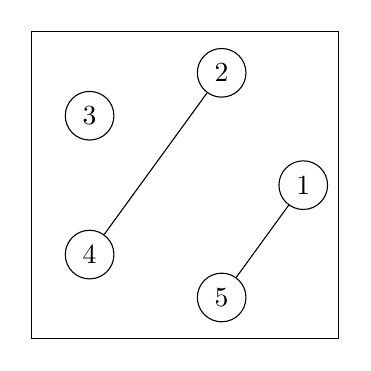
\begin{tikzpicture}
\tikzset{tinoeud/.style={draw, circle, minimum height=0.01cm}}
\clip (-2, -2) rectangle (2, 2);
\draw (-1.95, -1.95) rectangle (1.95, 1.95);
\node[tinoeud] (V1) at (0:1.5cm) {1};
\node[tinoeud] (V2) at (72:1.5cm) {2};
\node[tinoeud] (V3) at (144:1.5cm) {3};
\node[tinoeud] (V4) at (216:1.5cm) {4};
\node[tinoeud] (V5) at (288:1.5cm) {5};
\draw (V1) -- (V5);
\draw (V2) -- (V4);
\end{tikzpicture}
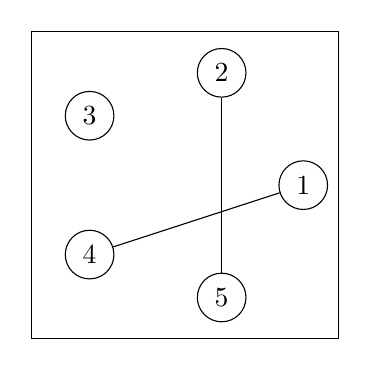
\begin{tikzpicture}
\tikzset{tinoeud/.style={draw, circle, minimum height=0.01cm}}
\clip (-2, -2) rectangle (2, 2);
\draw (-1.95, -1.95) rectangle (1.95, 1.95);
\node[tinoeud] (V1) at (0:1.5cm) {1};
\node[tinoeud] (V2) at (72:1.5cm) {2};
\node[tinoeud] (V3) at (144:1.5cm) {3};
\node[tinoeud] (V4) at (216:1.5cm) {4};
\node[tinoeud] (V5) at (288:1.5cm) {5};
\draw (V1) -- (V4);
\draw (V2) -- (V5);
\end{tikzpicture}
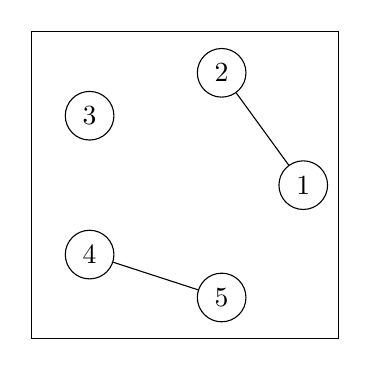
\begin{tikzpicture}
\tikzset{tinoeud/.style={draw, circle, minimum height=0.01cm}}
\clip (-2, -2) rectangle (2, 2);
\draw (-1.95, -1.95) rectangle (1.95, 1.95);
\node[tinoeud] (V1) at (0:1.5cm) {1};
\node[tinoeud] (V2) at (72:1.5cm) {2};
\node[tinoeud] (V3) at (144:1.5cm) {3};
\node[tinoeud] (V4) at (216:1.5cm) {4};
\node[tinoeud] (V5) at (288:1.5cm) {5};
\draw (V1) -- (V2);
\draw (V4) -- (V5);
\end{tikzpicture}
\\
\newpage
classe de la partition grosse
\\
\begin{tabular}{c c c c c c}
\toprule 
Noeuds & Requête & Noeuds & Requête & Noeuds & Requête \\
\midrule 
1, 2, 3, 4 & 2.0 & 1, 2, 3, 5 & 1.0 & 1, 2, 4, 5 & 3.0 \\
1, 3, 4, 5 & 2.0 & 2, 3, 4, 5 & 1.0 \\
\bottomrule 
\end{tabular}
\\
\begin{center}
classe de la partition fine
\\
\begin{tabular}{c c c c c c}
\toprule 
Noeuds & Requête & Noeuds & Requête & Noeuds & Requête \\
\midrule 
1, 2, 3, 4 & 4 & 1, 2, 3, 5 & 2 & 1, 2, 4, 5 & 11 \\
1, 3, 4, 5 & 4 & 2, 3, 4, 5 & 2 \\
\bottomrule 
\end{tabular}
\end{center}
\\
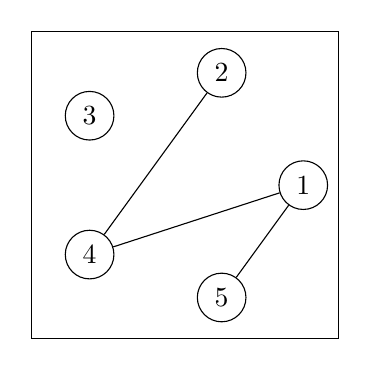
\begin{tikzpicture}
\tikzset{tinoeud/.style={draw, circle, minimum height=0.01cm}}
\clip (-2, -2) rectangle (2, 2);
\draw (-1.95, -1.95) rectangle (1.95, 1.95);
\node[tinoeud] (V1) at (0:1.5cm) {1};
\node[tinoeud] (V2) at (72:1.5cm) {2};
\node[tinoeud] (V3) at (144:1.5cm) {3};
\node[tinoeud] (V4) at (216:1.5cm) {4};
\node[tinoeud] (V5) at (288:1.5cm) {5};
\draw (V1) -- (V4);
\draw (V1) -- (V5);
\draw (V2) -- (V4);
\end{tikzpicture}
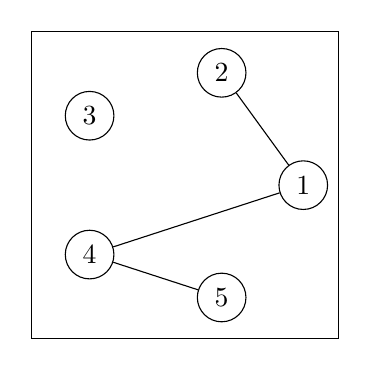
\begin{tikzpicture}
\tikzset{tinoeud/.style={draw, circle, minimum height=0.01cm}}
\clip (-2, -2) rectangle (2, 2);
\draw (-1.95, -1.95) rectangle (1.95, 1.95);
\node[tinoeud] (V1) at (0:1.5cm) {1};
\node[tinoeud] (V2) at (72:1.5cm) {2};
\node[tinoeud] (V3) at (144:1.5cm) {3};
\node[tinoeud] (V4) at (216:1.5cm) {4};
\node[tinoeud] (V5) at (288:1.5cm) {5};
\draw (V1) -- (V2);
\draw (V1) -- (V4);
\draw (V4) -- (V5);
\end{tikzpicture}
\newpage
classe de la partition grosse
\\
\begin{tabular}{c c c c c c}
\toprule 
Noeuds & Requête & Noeuds & Requête & Noeuds & Requête \\
\midrule 
1, 2, 3, 4 & 1.0 & 1, 2, 3, 5 & 2.0 & 1, 2, 4, 5 & 1.0 \\
1, 3, 4, 5 & 3.0 & 2, 3, 4, 5 & 2.0 \\
\bottomrule 
\end{tabular}
\\
\begin{center}
classe de la partition fine
\\
\begin{tabular}{c c c c c c}
\toprule 
Noeuds & Requête & Noeuds & Requête & Noeuds & Requête \\
\midrule 
1, 2, 3, 4 & 2 & 1, 2, 3, 5 & 4 & 1, 2, 4, 5 & 2 \\
1, 3, 4, 5 & 11 & 2, 3, 4, 5 & 4 \\
\bottomrule 
\end{tabular}
\end{center}
\\
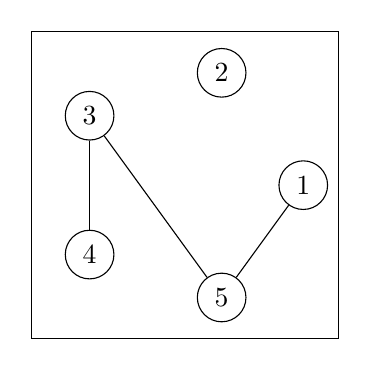
\begin{tikzpicture}
\tikzset{tinoeud/.style={draw, circle, minimum height=0.01cm}}
\clip (-2, -2) rectangle (2, 2);
\draw (-1.95, -1.95) rectangle (1.95, 1.95);
\node[tinoeud] (V1) at (0:1.5cm) {1};
\node[tinoeud] (V2) at (72:1.5cm) {2};
\node[tinoeud] (V3) at (144:1.5cm) {3};
\node[tinoeud] (V4) at (216:1.5cm) {4};
\node[tinoeud] (V5) at (288:1.5cm) {5};
\draw (V1) -- (V5);
\draw (V3) -- (V4);
\draw (V3) -- (V5);
\end{tikzpicture}
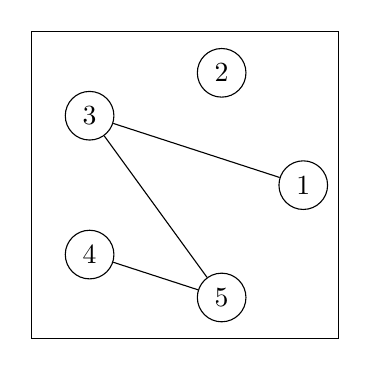
\begin{tikzpicture}
\tikzset{tinoeud/.style={draw, circle, minimum height=0.01cm}}
\clip (-2, -2) rectangle (2, 2);
\draw (-1.95, -1.95) rectangle (1.95, 1.95);
\node[tinoeud] (V1) at (0:1.5cm) {1};
\node[tinoeud] (V2) at (72:1.5cm) {2};
\node[tinoeud] (V3) at (144:1.5cm) {3};
\node[tinoeud] (V4) at (216:1.5cm) {4};
\node[tinoeud] (V5) at (288:1.5cm) {5};
\draw (V1) -- (V3);
\draw (V3) -- (V5);
\draw (V4) -- (V5);
\end{tikzpicture}
\newpage
classe de la partition grosse
\\
\begin{tabular}{c c c c c c}
\toprule 
Noeuds & Requête & Noeuds & Requête & Noeuds & Requête \\
\midrule 
1, 2, 3, 4 & 2.0 & 1, 2, 3, 5 & 4.0 & 1, 2, 4, 5 & 2.0 \\
1, 3, 4, 5 & 3.0 & 2, 3, 4, 5 & 4.0 \\
\bottomrule 
\end{tabular}
\\
\begin{center}
classe de la partition fine
\\
\begin{tabular}{c c c c c c}
\toprule 
Noeuds & Requête & Noeuds & Requête & Noeuds & Requête \\
\midrule 
1, 2, 3, 4 & 4 & 1, 2, 3, 5 & 5 & 1, 2, 4, 5 & 4 \\
1, 3, 4, 5 & 11 & 2, 3, 4, 5 & 5 \\
\bottomrule 
\end{tabular}
\end{center}
\\
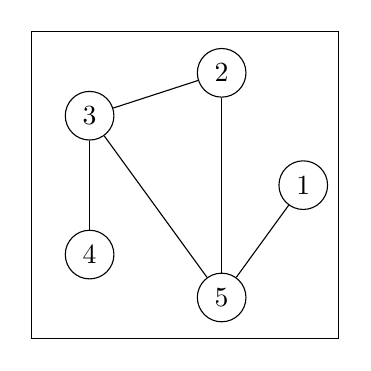
\begin{tikzpicture}
\tikzset{tinoeud/.style={draw, circle, minimum height=0.01cm}}
\clip (-2, -2) rectangle (2, 2);
\draw (-1.95, -1.95) rectangle (1.95, 1.95);
\node[tinoeud] (V1) at (0:1.5cm) {1};
\node[tinoeud] (V2) at (72:1.5cm) {2};
\node[tinoeud] (V3) at (144:1.5cm) {3};
\node[tinoeud] (V4) at (216:1.5cm) {4};
\node[tinoeud] (V5) at (288:1.5cm) {5};
\draw (V1) -- (V5);
\draw (V2) -- (V3);
\draw (V2) -- (V5);
\draw (V3) -- (V4);
\draw (V3) -- (V5);
\end{tikzpicture}
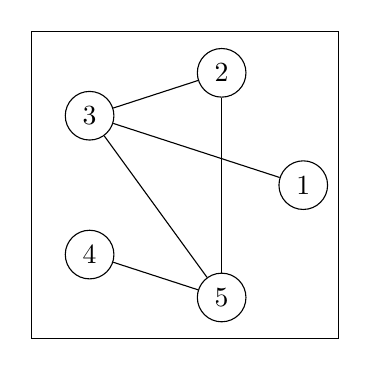
\begin{tikzpicture}
\tikzset{tinoeud/.style={draw, circle, minimum height=0.01cm}}
\clip (-2, -2) rectangle (2, 2);
\draw (-1.95, -1.95) rectangle (1.95, 1.95);
\node[tinoeud] (V1) at (0:1.5cm) {1};
\node[tinoeud] (V2) at (72:1.5cm) {2};
\node[tinoeud] (V3) at (144:1.5cm) {3};
\node[tinoeud] (V4) at (216:1.5cm) {4};
\node[tinoeud] (V5) at (288:1.5cm) {5};
\draw (V1) -- (V3);
\draw (V2) -- (V3);
\draw (V2) -- (V5);
\draw (V3) -- (V5);
\draw (V4) -- (V5);
\end{tikzpicture}
\newpage
classe de la partition grosse
\\
\begin{tabular}{c c c c c c}
\toprule 
Noeuds & Requête & Noeuds & Requête & Noeuds & Requête \\
\midrule 
1, 2, 3, 4 & 3.0 & 1, 2, 3, 5 & 5.0 & 1, 2, 4, 5 & 4.0 \\
1, 3, 4, 5 & 3.0 & 2, 3, 4, 5 & 3.0 \\
\bottomrule 
\end{tabular}
\\
\begin{center}
classe de la partition fine
\\
\begin{tabular}{c c c c c c}
\toprule 
Noeuds & Requête & Noeuds & Requête & Noeuds & Requête \\
\midrule 
1, 2, 3, 4 & 11 & 1, 2, 3, 5 & 3 & 1, 2, 4, 5 & 5 \\
1, 3, 4, 5 & 11 & 2, 3, 4, 5 & 9 \\
\bottomrule 
\end{tabular}
\end{center}
\\
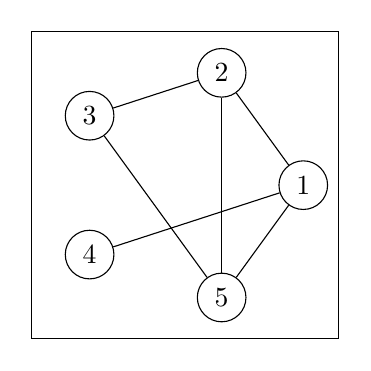
\begin{tikzpicture}
\tikzset{tinoeud/.style={draw, circle, minimum height=0.01cm}}
\clip (-2, -2) rectangle (2, 2);
\draw (-1.95, -1.95) rectangle (1.95, 1.95);
\node[tinoeud] (V1) at (0:1.5cm) {1};
\node[tinoeud] (V2) at (72:1.5cm) {2};
\node[tinoeud] (V3) at (144:1.5cm) {3};
\node[tinoeud] (V4) at (216:1.5cm) {4};
\node[tinoeud] (V5) at (288:1.5cm) {5};
\draw (V1) -- (V2);
\draw (V1) -- (V4);
\draw (V1) -- (V5);
\draw (V2) -- (V3);
\draw (V2) -- (V5);
\draw (V3) -- (V5);
\end{tikzpicture}
\begin{center}
classe de la partition fine
\\
\begin{tabular}{c c c c c c}
\toprule 
Noeuds & Requête & Noeuds & Requête & Noeuds & Requête \\
\midrule 
1, 2, 3, 4 & 11 & 1, 2, 3, 5 & 3 & 1, 2, 4, 5 & 5 \\
1, 3, 4, 5 & 9 & 2, 3, 4, 5 & 11 \\
\bottomrule 
\end{tabular}
\end{center}
\\
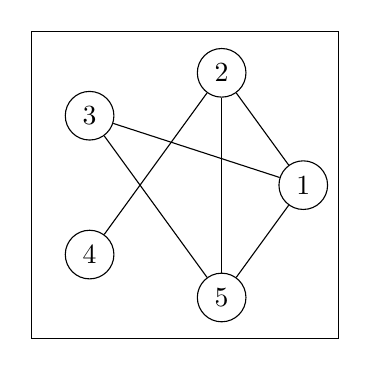
\begin{tikzpicture}
\tikzset{tinoeud/.style={draw, circle, minimum height=0.01cm}}
\clip (-2, -2) rectangle (2, 2);
\draw (-1.95, -1.95) rectangle (1.95, 1.95);
\node[tinoeud] (V1) at (0:1.5cm) {1};
\node[tinoeud] (V2) at (72:1.5cm) {2};
\node[tinoeud] (V3) at (144:1.5cm) {3};
\node[tinoeud] (V4) at (216:1.5cm) {4};
\node[tinoeud] (V5) at (288:1.5cm) {5};
\draw (V1) -- (V2);
\draw (V1) -- (V3);
\draw (V1) -- (V5);
\draw (V2) -- (V4);
\draw (V2) -- (V5);
\draw (V3) -- (V5);
\end{tikzpicture}
\newpage
\begin{center}
classe de la partition fine
\\
\begin{tabular}{c c c c c c}
\toprule 
Noeuds & Requête & Noeuds & Requête & Noeuds & Requête \\
\midrule 
1, 2, 3, 4 & 9 & 1, 2, 3, 5 & 3 & 1, 2, 4, 5 & 5 \\
1, 3, 4, 5 & 11 & 2, 3, 4, 5 & 11 \\
\bottomrule 
\end{tabular}
\end{center}
\\
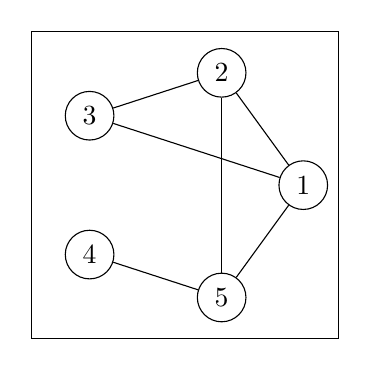
\begin{tikzpicture}
\tikzset{tinoeud/.style={draw, circle, minimum height=0.01cm}}
\clip (-2, -2) rectangle (2, 2);
\draw (-1.95, -1.95) rectangle (1.95, 1.95);
\node[tinoeud] (V1) at (0:1.5cm) {1};
\node[tinoeud] (V2) at (72:1.5cm) {2};
\node[tinoeud] (V3) at (144:1.5cm) {3};
\node[tinoeud] (V4) at (216:1.5cm) {4};
\node[tinoeud] (V5) at (288:1.5cm) {5};
\draw (V1) -- (V2);
\draw (V1) -- (V3);
\draw (V1) -- (V5);
\draw (V2) -- (V3);
\draw (V2) -- (V5);
\draw (V4) -- (V5);
\end{tikzpicture}
\newpage
classe de la partition grosse
\\
\begin{tabular}{c c c c c c}
\toprule 
Noeuds & Requête & Noeuds & Requête & Noeuds & Requête \\
\midrule 
1, 2, 3, 4 & 2.0 & 1, 2, 3, 5 & 2.0 & 1, 2, 4, 5 & 3.0 \\
1, 3, 4, 5 & 1.0 & 2, 3, 4, 5 & 1.0 \\
\bottomrule 
\end{tabular}
\\
\begin{center}
classe de la partition fine
\\
\begin{tabular}{c c c c c c}
\toprule 
Noeuds & Requête & Noeuds & Requête & Noeuds & Requête \\
\midrule 
1, 2, 3, 4 & 4 & 1, 2, 3, 5 & 4 & 1, 2, 4, 5 & 11 \\
1, 3, 4, 5 & 2 & 2, 3, 4, 5 & 2 \\
\bottomrule 
\end{tabular}
\end{center}
\\
\begin{tikzpicture}
\tikzset{tinoeud/.style={draw, circle, minimum height=0.01cm}}
\clip (-2, -2) rectangle (2, 2);
\draw (-1.95, -1.95) rectangle (1.95, 1.95);
\node[tinoeud] (V1) at (0:1.5cm) {1};
\node[tinoeud] (V2) at (72:1.5cm) {2};
\node[tinoeud] (V3) at (144:1.5cm) {3};
\node[tinoeud] (V4) at (216:1.5cm) {4};
\node[tinoeud] (V5) at (288:1.5cm) {5};
\draw (V1) -- (V2);
\draw (V1) -- (V5);
\draw (V2) -- (V4);
\end{tikzpicture}
\begin{tikzpicture}
\tikzset{tinoeud/.style={draw, circle, minimum height=0.01cm}}
\clip (-2, -2) rectangle (2, 2);
\draw (-1.95, -1.95) rectangle (1.95, 1.95);
\node[tinoeud] (V1) at (0:1.5cm) {1};
\node[tinoeud] (V2) at (72:1.5cm) {2};
\node[tinoeud] (V3) at (144:1.5cm) {3};
\node[tinoeud] (V4) at (216:1.5cm) {4};
\node[tinoeud] (V5) at (288:1.5cm) {5};
\draw (V1) -- (V2);
\draw (V1) -- (V4);
\draw (V2) -- (V5);
\end{tikzpicture}
\newpage
classe de la partition grosse
\\
\begin{tabular}{c c c c c c}
\toprule 
Noeuds & Requête & Noeuds & Requête & Noeuds & Requête \\
\midrule 
1, 2, 3, 4 & 4.0 & 1, 2, 3, 5 & 4.0 & 1, 2, 4, 5 & 4.0 \\
1, 3, 4, 5 & 5.0 & 2, 3, 4, 5 & 4.0 \\
\bottomrule 
\end{tabular}
\\
\begin{center}
classe de la partition fine
\\
\begin{tabular}{c c c c c c}
\toprule 
Noeuds & Requête & Noeuds & Requête & Noeuds & Requête \\
\midrule 
1, 2, 3, 4 & 5 & 1, 2, 3, 5 & 5 & 1, 2, 4, 5 & 8 \\
1, 3, 4, 5 & 3 & 2, 3, 4, 5 & 8 \\
\bottomrule 
\end{tabular}
\end{center}
\\
\begin{tikzpicture}
\tikzset{tinoeud/.style={draw, circle, minimum height=0.01cm}}
\clip (-2, -2) rectangle (2, 2);
\draw (-1.95, -1.95) rectangle (1.95, 1.95);
\node[tinoeud] (V1) at (0:1.5cm) {1};
\node[tinoeud] (V2) at (72:1.5cm) {2};
\node[tinoeud] (V3) at (144:1.5cm) {3};
\node[tinoeud] (V4) at (216:1.5cm) {4};
\node[tinoeud] (V5) at (288:1.5cm) {5};
\draw (V1) -- (V3);
\draw (V1) -- (V4);
\draw (V1) -- (V5);
\draw (V2) -- (V4);
\draw (V2) -- (V5);
\draw (V3) -- (V4);
\draw (V3) -- (V5);
\end{tikzpicture}
\begin{center}
classe de la partition fine
\\
\begin{tabular}{c c c c c c}
\toprule 
Noeuds & Requête & Noeuds & Requête & Noeuds & Requête \\
\midrule 
1, 2, 3, 4 & 5 & 1, 2, 3, 5 & 8 & 1, 2, 4, 5 & 5 \\
1, 3, 4, 5 & 3 & 2, 3, 4, 5 & 8 \\
\bottomrule 
\end{tabular}
\end{center}
\\
\begin{tikzpicture}
\tikzset{tinoeud/.style={draw, circle, minimum height=0.01cm}}
\clip (-2, -2) rectangle (2, 2);
\draw (-1.95, -1.95) rectangle (1.95, 1.95);
\node[tinoeud] (V1) at (0:1.5cm) {1};
\node[tinoeud] (V2) at (72:1.5cm) {2};
\node[tinoeud] (V3) at (144:1.5cm) {3};
\node[tinoeud] (V4) at (216:1.5cm) {4};
\node[tinoeud] (V5) at (288:1.5cm) {5};
\draw (V1) -- (V3);
\draw (V1) -- (V4);
\draw (V1) -- (V5);
\draw (V2) -- (V3);
\draw (V2) -- (V5);
\draw (V3) -- (V4);
\draw (V4) -- (V5);
\end{tikzpicture}
\newpage
\begin{center}
classe de la partition fine
\\
\begin{tabular}{c c c c c c}
\toprule 
Noeuds & Requête & Noeuds & Requête & Noeuds & Requête \\
\midrule 
1, 2, 3, 4 & 8 & 1, 2, 3, 5 & 5 & 1, 2, 4, 5 & 5 \\
1, 3, 4, 5 & 3 & 2, 3, 4, 5 & 8 \\
\bottomrule 
\end{tabular}
\end{center}
\\
\begin{tikzpicture}
\tikzset{tinoeud/.style={draw, circle, minimum height=0.01cm}}
\clip (-2, -2) rectangle (2, 2);
\draw (-1.95, -1.95) rectangle (1.95, 1.95);
\node[tinoeud] (V1) at (0:1.5cm) {1};
\node[tinoeud] (V2) at (72:1.5cm) {2};
\node[tinoeud] (V3) at (144:1.5cm) {3};
\node[tinoeud] (V4) at (216:1.5cm) {4};
\node[tinoeud] (V5) at (288:1.5cm) {5};
\draw (V1) -- (V3);
\draw (V1) -- (V4);
\draw (V1) -- (V5);
\draw (V2) -- (V3);
\draw (V2) -- (V4);
\draw (V3) -- (V5);
\draw (V4) -- (V5);
\end{tikzpicture}
\begin{center}
classe de la partition fine
\\
\begin{tabular}{c c c c c c}
\toprule 
Noeuds & Requête & Noeuds & Requête & Noeuds & Requête \\
\midrule 
1, 2, 3, 4 & 8 & 1, 2, 3, 5 & 8 & 1, 2, 4, 5 & 5 \\
1, 3, 4, 5 & 3 & 2, 3, 4, 5 & 5 \\
\bottomrule 
\end{tabular}
\end{center}
\\
\begin{tikzpicture}
\tikzset{tinoeud/.style={draw, circle, minimum height=0.01cm}}
\clip (-2, -2) rectangle (2, 2);
\draw (-1.95, -1.95) rectangle (1.95, 1.95);
\node[tinoeud] (V1) at (0:1.5cm) {1};
\node[tinoeud] (V2) at (72:1.5cm) {2};
\node[tinoeud] (V3) at (144:1.5cm) {3};
\node[tinoeud] (V4) at (216:1.5cm) {4};
\node[tinoeud] (V5) at (288:1.5cm) {5};
\draw (V1) -- (V2);
\draw (V1) -- (V4);
\draw (V1) -- (V5);
\draw (V2) -- (V3);
\draw (V3) -- (V4);
\draw (V3) -- (V5);
\draw (V4) -- (V5);
\end{tikzpicture}
\newpage
\begin{center}
classe de la partition fine
\\
\begin{tabular}{c c c c c c}
\toprule 
Noeuds & Requête & Noeuds & Requête & Noeuds & Requête \\
\midrule 
1, 2, 3, 4 & 8 & 1, 2, 3, 5 & 5 & 1, 2, 4, 5 & 8 \\
1, 3, 4, 5 & 3 & 2, 3, 4, 5 & 5 \\
\bottomrule 
\end{tabular}
\end{center}
\\
\begin{tikzpicture}
\tikzset{tinoeud/.style={draw, circle, minimum height=0.01cm}}
\clip (-2, -2) rectangle (2, 2);
\draw (-1.95, -1.95) rectangle (1.95, 1.95);
\node[tinoeud] (V1) at (0:1.5cm) {1};
\node[tinoeud] (V2) at (72:1.5cm) {2};
\node[tinoeud] (V3) at (144:1.5cm) {3};
\node[tinoeud] (V4) at (216:1.5cm) {4};
\node[tinoeud] (V5) at (288:1.5cm) {5};
\draw (V1) -- (V2);
\draw (V1) -- (V3);
\draw (V1) -- (V5);
\draw (V2) -- (V4);
\draw (V3) -- (V4);
\draw (V3) -- (V5);
\draw (V4) -- (V5);
\end{tikzpicture}
\begin{center}
classe de la partition fine
\\
\begin{tabular}{c c c c c c}
\toprule 
Noeuds & Requête & Noeuds & Requête & Noeuds & Requête \\
\midrule 
1, 2, 3, 4 & 5 & 1, 2, 3, 5 & 8 & 1, 2, 4, 5 & 8 \\
1, 3, 4, 5 & 3 & 2, 3, 4, 5 & 5 \\
\bottomrule 
\end{tabular}
\end{center}
\\
\begin{tikzpicture}
\tikzset{tinoeud/.style={draw, circle, minimum height=0.01cm}}
\clip (-2, -2) rectangle (2, 2);
\draw (-1.95, -1.95) rectangle (1.95, 1.95);
\node[tinoeud] (V1) at (0:1.5cm) {1};
\node[tinoeud] (V2) at (72:1.5cm) {2};
\node[tinoeud] (V3) at (144:1.5cm) {3};
\node[tinoeud] (V4) at (216:1.5cm) {4};
\node[tinoeud] (V5) at (288:1.5cm) {5};
\draw (V1) -- (V2);
\draw (V1) -- (V3);
\draw (V1) -- (V4);
\draw (V2) -- (V5);
\draw (V3) -- (V4);
\draw (V3) -- (V5);
\draw (V4) -- (V5);
\end{tikzpicture}
\newpage
\newpage
classe de la partition grosse
\\
\begin{tabular}{c c c c c c}
\toprule 
Noeuds & Requête & Noeuds & Requête & Noeuds & Requête \\
\midrule 
1, 2, 3, 4 & 3.0 & 1, 2, 3, 5 & 2.0 & 1, 2, 4, 5 & 4.0 \\
1, 3, 4, 5 & 3.0 & 2, 3, 4, 5 & 3.0 \\
\bottomrule 
\end{tabular}
\\
\begin{center}
classe de la partition fine
\\
\begin{tabular}{c c c c c c}
\toprule 
Noeuds & Requête & Noeuds & Requête & Noeuds & Requête \\
\midrule 
1, 2, 3, 4 & 10 & 1, 2, 3, 5 & 4 & 1, 2, 4, 5 & 8 \\
1, 3, 4, 5 & 11 & 2, 3, 4, 5 & 11 \\
\bottomrule 
\end{tabular}
\end{center}
\\
\begin{tikzpicture}
\tikzset{tinoeud/.style={draw, circle, minimum height=0.01cm}}
\clip (-2, -2) rectangle (2, 2);
\draw (-1.95, -1.95) rectangle (1.95, 1.95);
\node[tinoeud] (V1) at (0:1.5cm) {1};
\node[tinoeud] (V2) at (72:1.5cm) {2};
\node[tinoeud] (V3) at (144:1.5cm) {3};
\node[tinoeud] (V4) at (216:1.5cm) {4};
\node[tinoeud] (V5) at (288:1.5cm) {5};
\draw (V1) -- (V4);
\draw (V1) -- (V5);
\draw (V2) -- (V4);
\draw (V2) -- (V5);
\draw (V3) -- (V4);
\end{tikzpicture}
\begin{center}
classe de la partition fine
\\
\begin{tabular}{c c c c c c}
\toprule 
Noeuds & Requête & Noeuds & Requête & Noeuds & Requête \\
\midrule 
1, 2, 3, 4 & 11 & 1, 2, 3, 5 & 7 & 1, 2, 4, 5 & 5 \\
1, 3, 4, 5 & 9 & 2, 3, 4, 5 & 11 \\
\bottomrule 
\end{tabular}
\end{center}
\\
\begin{tikzpicture}
\tikzset{tinoeud/.style={draw, circle, minimum height=0.01cm}}
\clip (-2, -2) rectangle (2, 2);
\draw (-1.95, -1.95) rectangle (1.95, 1.95);
\node[tinoeud] (V1) at (0:1.5cm) {1};
\node[tinoeud] (V2) at (72:1.5cm) {2};
\node[tinoeud] (V3) at (144:1.5cm) {3};
\node[tinoeud] (V4) at (216:1.5cm) {4};
\node[tinoeud] (V5) at (288:1.5cm) {5};
\draw (V1) -- (V4);
\draw (V1) -- (V5);
\draw (V2) -- (V3);
\draw (V2) -- (V4);
\draw (V4) -- (V5);
\end{tikzpicture}
\newpage
\begin{center}
classe de la partition fine
\\
\begin{tabular}{c c c c c c}
\toprule 
Noeuds & Requête & Noeuds & Requête & Noeuds & Requête \\
\midrule 
1, 2, 3, 4 & 11 & 1, 2, 3, 5 & 7 & 1, 2, 4, 5 & 5 \\
1, 3, 4, 5 & 11 & 2, 3, 4, 5 & 9 \\
\bottomrule 
\end{tabular}
\end{center}
\\
\begin{tikzpicture}
\tikzset{tinoeud/.style={draw, circle, minimum height=0.01cm}}
\clip (-2, -2) rectangle (2, 2);
\draw (-1.95, -1.95) rectangle (1.95, 1.95);
\node[tinoeud] (V1) at (0:1.5cm) {1};
\node[tinoeud] (V2) at (72:1.5cm) {2};
\node[tinoeud] (V3) at (144:1.5cm) {3};
\node[tinoeud] (V4) at (216:1.5cm) {4};
\node[tinoeud] (V5) at (288:1.5cm) {5};
\draw (V1) -- (V3);
\draw (V1) -- (V4);
\draw (V2) -- (V4);
\draw (V2) -- (V5);
\draw (V4) -- (V5);
\end{tikzpicture}
\begin{center}
classe de la partition fine
\\
\begin{tabular}{c c c c c c}
\toprule 
Noeuds & Requête & Noeuds & Requête & Noeuds & Requête \\
\midrule 
1, 2, 3, 4 & 11 & 1, 2, 3, 5 & 4 & 1, 2, 4, 5 & 8 \\
1, 3, 4, 5 & 11 & 2, 3, 4, 5 & 10 \\
\bottomrule 
\end{tabular}
\end{center}
\\
\begin{tikzpicture}
\tikzset{tinoeud/.style={draw, circle, minimum height=0.01cm}}
\clip (-2, -2) rectangle (2, 2);
\draw (-1.95, -1.95) rectangle (1.95, 1.95);
\node[tinoeud] (V1) at (0:1.5cm) {1};
\node[tinoeud] (V2) at (72:1.5cm) {2};
\node[tinoeud] (V3) at (144:1.5cm) {3};
\node[tinoeud] (V4) at (216:1.5cm) {4};
\node[tinoeud] (V5) at (288:1.5cm) {5};
\draw (V1) -- (V2);
\draw (V1) -- (V5);
\draw (V2) -- (V4);
\draw (V3) -- (V4);
\draw (V4) -- (V5);
\end{tikzpicture}
\newpage
\begin{center}
classe de la partition fine
\\
\begin{tabular}{c c c c c c}
\toprule 
Noeuds & Requête & Noeuds & Requête & Noeuds & Requête \\
\midrule 
1, 2, 3, 4 & 11 & 1, 2, 3, 5 & 4 & 1, 2, 4, 5 & 8 \\
1, 3, 4, 5 & 10 & 2, 3, 4, 5 & 11 \\
\bottomrule 
\end{tabular}
\end{center}
\\
\begin{tikzpicture}
\tikzset{tinoeud/.style={draw, circle, minimum height=0.01cm}}
\clip (-2, -2) rectangle (2, 2);
\draw (-1.95, -1.95) rectangle (1.95, 1.95);
\node[tinoeud] (V1) at (0:1.5cm) {1};
\node[tinoeud] (V2) at (72:1.5cm) {2};
\node[tinoeud] (V3) at (144:1.5cm) {3};
\node[tinoeud] (V4) at (216:1.5cm) {4};
\node[tinoeud] (V5) at (288:1.5cm) {5};
\draw (V1) -- (V2);
\draw (V1) -- (V4);
\draw (V2) -- (V5);
\draw (V3) -- (V4);
\draw (V4) -- (V5);
\end{tikzpicture}
\begin{center}
classe de la partition fine
\\
\begin{tabular}{c c c c c c}
\toprule 
Noeuds & Requête & Noeuds & Requête & Noeuds & Requête \\
\midrule 
1, 2, 3, 4 & 9 & 1, 2, 3, 5 & 7 & 1, 2, 4, 5 & 5 \\
1, 3, 4, 5 & 11 & 2, 3, 4, 5 & 11 \\
\bottomrule 
\end{tabular}
\end{center}
\\
\begin{tikzpicture}
\tikzset{tinoeud/.style={draw, circle, minimum height=0.01cm}}
\clip (-2, -2) rectangle (2, 2);
\draw (-1.95, -1.95) rectangle (1.95, 1.95);
\node[tinoeud] (V1) at (0:1.5cm) {1};
\node[tinoeud] (V2) at (72:1.5cm) {2};
\node[tinoeud] (V3) at (144:1.5cm) {3};
\node[tinoeud] (V4) at (216:1.5cm) {4};
\node[tinoeud] (V5) at (288:1.5cm) {5};
\draw (V1) -- (V2);
\draw (V1) -- (V4);
\draw (V2) -- (V4);
\draw (V3) -- (V5);
\draw (V4) -- (V5);
\end{tikzpicture}
\newpage
\newpage
classe de la partition grosse
\\
\begin{tabular}{c c c c c c}
\toprule 
Noeuds & Requête & Noeuds & Requête & Noeuds & Requête \\
\midrule 
1, 2, 3, 4 & 5.0 & 1, 2, 3, 5 & 5.0 & 1, 2, 4, 5 & 3.0 \\
1, 3, 4, 5 & 4.0 & 2, 3, 4, 5 & 4.0 \\
\bottomrule 
\end{tabular}
\\
\begin{center}
classe de la partition fine
\\
\begin{tabular}{c c c c c c}
\toprule 
Noeuds & Requête & Noeuds & Requête & Noeuds & Requête \\
\midrule 
1, 2, 3, 4 & 3 & 1, 2, 3, 5 & 3 & 1, 2, 4, 5 & 11 \\
1, 3, 4, 5 & 5 & 2, 3, 4, 5 & 5 \\
\bottomrule 
\end{tabular}
\end{center}
\\
\begin{tikzpicture}
\tikzset{tinoeud/.style={draw, circle, minimum height=0.01cm}}
\clip (-2, -2) rectangle (2, 2);
\draw (-1.95, -1.95) rectangle (1.95, 1.95);
\node[tinoeud] (V1) at (0:1.5cm) {1};
\node[tinoeud] (V2) at (72:1.5cm) {2};
\node[tinoeud] (V3) at (144:1.5cm) {3};
\node[tinoeud] (V4) at (216:1.5cm) {4};
\node[tinoeud] (V5) at (288:1.5cm) {5};
\draw (V1) -- (V2);
\draw (V1) -- (V3);
\draw (V1) -- (V5);
\draw (V2) -- (V3);
\draw (V2) -- (V4);
\draw (V3) -- (V4);
\draw (V3) -- (V5);
\end{tikzpicture}
\begin{tikzpicture}
\tikzset{tinoeud/.style={draw, circle, minimum height=0.01cm}}
\clip (-2, -2) rectangle (2, 2);
\draw (-1.95, -1.95) rectangle (1.95, 1.95);
\node[tinoeud] (V1) at (0:1.5cm) {1};
\node[tinoeud] (V2) at (72:1.5cm) {2};
\node[tinoeud] (V3) at (144:1.5cm) {3};
\node[tinoeud] (V4) at (216:1.5cm) {4};
\node[tinoeud] (V5) at (288:1.5cm) {5};
\draw (V1) -- (V2);
\draw (V1) -- (V3);
\draw (V1) -- (V4);
\draw (V2) -- (V3);
\draw (V2) -- (V5);
\draw (V3) -- (V4);
\draw (V3) -- (V5);
\end{tikzpicture}
\newpage
classe de la partition grosse
\\
\begin{tabular}{c c c c c c}
\toprule 
Noeuds & Requête & Noeuds & Requête & Noeuds & Requête \\
\midrule 
1, 2, 3, 4 & 2.0 & 1, 2, 3, 5 & 3.0 & 1, 2, 4, 5 & 1.0 \\
1, 3, 4, 5 & 3.0 & 2, 3, 4, 5 & 3.0 \\
\bottomrule 
\end{tabular}
\\
\begin{center}
classe de la partition fine
\\
\begin{tabular}{c c c c c c}
\toprule 
Noeuds & Requête & Noeuds & Requête & Noeuds & Requête \\
\midrule 
1, 2, 3, 4 & 4 & 1, 2, 3, 5 & 11 & 1, 2, 4, 5 & 2 \\
1, 3, 4, 5 & 11 & 2, 3, 4, 5 & 10 \\
\bottomrule 
\end{tabular}
\end{center}
\\
\begin{tikzpicture}
\tikzset{tinoeud/.style={draw, circle, minimum height=0.01cm}}
\clip (-2, -2) rectangle (2, 2);
\draw (-1.95, -1.95) rectangle (1.95, 1.95);
\node[tinoeud] (V1) at (0:1.5cm) {1};
\node[tinoeud] (V2) at (72:1.5cm) {2};
\node[tinoeud] (V3) at (144:1.5cm) {3};
\node[tinoeud] (V4) at (216:1.5cm) {4};
\node[tinoeud] (V5) at (288:1.5cm) {5};
\draw (V1) -- (V5);
\draw (V2) -- (V3);
\draw (V3) -- (V4);
\draw (V3) -- (V5);
\end{tikzpicture}
\begin{center}
classe de la partition fine
\\
\begin{tabular}{c c c c c c}
\toprule 
Noeuds & Requête & Noeuds & Requête & Noeuds & Requête \\
\midrule 
1, 2, 3, 4 & 4 & 1, 2, 3, 5 & 11 & 1, 2, 4, 5 & 2 \\
1, 3, 4, 5 & 10 & 2, 3, 4, 5 & 11 \\
\bottomrule 
\end{tabular}
\end{center}
\\
\begin{tikzpicture}
\tikzset{tinoeud/.style={draw, circle, minimum height=0.01cm}}
\clip (-2, -2) rectangle (2, 2);
\draw (-1.95, -1.95) rectangle (1.95, 1.95);
\node[tinoeud] (V1) at (0:1.5cm) {1};
\node[tinoeud] (V2) at (72:1.5cm) {2};
\node[tinoeud] (V3) at (144:1.5cm) {3};
\node[tinoeud] (V4) at (216:1.5cm) {4};
\node[tinoeud] (V5) at (288:1.5cm) {5};
\draw (V1) -- (V3);
\draw (V2) -- (V5);
\draw (V3) -- (V4);
\draw (V3) -- (V5);
\end{tikzpicture}
\newpage
\begin{center}
classe de la partition fine
\\
\begin{tabular}{c c c c c c}
\toprule 
Noeuds & Requête & Noeuds & Requête & Noeuds & Requête \\
\midrule 
1, 2, 3, 4 & 4 & 1, 2, 3, 5 & 10 & 1, 2, 4, 5 & 2 \\
1, 3, 4, 5 & 11 & 2, 3, 4, 5 & 11 \\
\bottomrule 
\end{tabular}
\end{center}
\\
\begin{tikzpicture}
\tikzset{tinoeud/.style={draw, circle, minimum height=0.01cm}}
\clip (-2, -2) rectangle (2, 2);
\draw (-1.95, -1.95) rectangle (1.95, 1.95);
\node[tinoeud] (V1) at (0:1.5cm) {1};
\node[tinoeud] (V2) at (72:1.5cm) {2};
\node[tinoeud] (V3) at (144:1.5cm) {3};
\node[tinoeud] (V4) at (216:1.5cm) {4};
\node[tinoeud] (V5) at (288:1.5cm) {5};
\draw (V1) -- (V3);
\draw (V2) -- (V3);
\draw (V3) -- (V5);
\draw (V4) -- (V5);
\end{tikzpicture}
\newpage
classe de la partition grosse
\\
\begin{tabular}{c c c c c c}
\toprule 
Noeuds & Requête & Noeuds & Requête & Noeuds & Requête \\
\midrule 
1, 2, 3, 4 & 3.0 & 1, 2, 3, 5 & 4.0 & 1, 2, 4, 5 & 4.0 \\
1, 3, 4, 5 & 5.0 & 2, 3, 4, 5 & 5.0 \\
\bottomrule 
\end{tabular}
\\
\begin{center}
classe de la partition fine
\\
\begin{tabular}{c c c c c c}
\toprule 
Noeuds & Requête & Noeuds & Requête & Noeuds & Requête \\
\midrule 
1, 2, 3, 4 & 11 & 1, 2, 3, 5 & 5 & 1, 2, 4, 5 & 5 \\
1, 3, 4, 5 & 3 & 2, 3, 4, 5 & 3 \\
\bottomrule 
\end{tabular}
\end{center}
\\
\begin{tikzpicture}
\tikzset{tinoeud/.style={draw, circle, minimum height=0.01cm}}
\clip (-2, -2) rectangle (2, 2);
\draw (-1.95, -1.95) rectangle (1.95, 1.95);
\node[tinoeud] (V1) at (0:1.5cm) {1};
\node[tinoeud] (V2) at (72:1.5cm) {2};
\node[tinoeud] (V3) at (144:1.5cm) {3};
\node[tinoeud] (V4) at (216:1.5cm) {4};
\node[tinoeud] (V5) at (288:1.5cm) {5};
\draw (V1) -- (V4);
\draw (V1) -- (V5);
\draw (V2) -- (V3);
\draw (V2) -- (V5);
\draw (V3) -- (V4);
\draw (V3) -- (V5);
\draw (V4) -- (V5);
\end{tikzpicture}
\begin{tikzpicture}
\tikzset{tinoeud/.style={draw, circle, minimum height=0.01cm}}
\clip (-2, -2) rectangle (2, 2);
\draw (-1.95, -1.95) rectangle (1.95, 1.95);
\node[tinoeud] (V1) at (0:1.5cm) {1};
\node[tinoeud] (V2) at (72:1.5cm) {2};
\node[tinoeud] (V3) at (144:1.5cm) {3};
\node[tinoeud] (V4) at (216:1.5cm) {4};
\node[tinoeud] (V5) at (288:1.5cm) {5};
\draw (V1) -- (V3);
\draw (V1) -- (V5);
\draw (V2) -- (V4);
\draw (V2) -- (V5);
\draw (V3) -- (V4);
\draw (V3) -- (V5);
\draw (V4) -- (V5);
\end{tikzpicture}
\newpage
classe de la partition grosse
\\
\begin{tabular}{c c c c c c}
\toprule 
Noeuds & Requête & Noeuds & Requête & Noeuds & Requête \\
\midrule 
1, 2, 3, 4 & 4.0 & 1, 2, 3, 5 & 4.0 & 1, 2, 4, 5 & 4.0 \\
1, 3, 4, 5 & 3.0 & 2, 3, 4, 5 & 3.0 \\
\bottomrule 
\end{tabular}
\\
\begin{center}
classe de la partition fine
\\
\begin{tabular}{c c c c c c}
\toprule 
Noeuds & Requête & Noeuds & Requête & Noeuds & Requête \\
\midrule 
1, 2, 3, 4 & 8 & 1, 2, 3, 5 & 8 & 1, 2, 4, 5 & 8 \\
1, 3, 4, 5 & 10 & 2, 3, 4, 5 & 10 \\
\bottomrule 
\end{tabular}
\end{center}
\\
\begin{tikzpicture}
\tikzset{tinoeud/.style={draw, circle, minimum height=0.01cm}}
\clip (-2, -2) rectangle (2, 2);
\draw (-1.95, -1.95) rectangle (1.95, 1.95);
\node[tinoeud] (V1) at (0:1.5cm) {1};
\node[tinoeud] (V2) at (72:1.5cm) {2};
\node[tinoeud] (V3) at (144:1.5cm) {3};
\node[tinoeud] (V4) at (216:1.5cm) {4};
\node[tinoeud] (V5) at (288:1.5cm) {5};
\draw (V1) -- (V3);
\draw (V1) -- (V4);
\draw (V1) -- (V5);
\draw (V2) -- (V3);
\draw (V2) -- (V4);
\draw (V2) -- (V5);
\end{tikzpicture}
\begin{center}
classe de la partition fine
\\
\begin{tabular}{c c c c c c}
\toprule 
Noeuds & Requête & Noeuds & Requête & Noeuds & Requête \\
\midrule 
1, 2, 3, 4 & 8 & 1, 2, 3, 5 & 5 & 1, 2, 4, 5 & 5 \\
1, 3, 4, 5 & 11 & 2, 3, 4, 5 & 11 \\
\bottomrule 
\end{tabular}
\end{center}
\\
\begin{tikzpicture}
\tikzset{tinoeud/.style={draw, circle, minimum height=0.01cm}}
\clip (-2, -2) rectangle (2, 2);
\draw (-1.95, -1.95) rectangle (1.95, 1.95);
\node[tinoeud] (V1) at (0:1.5cm) {1};
\node[tinoeud] (V2) at (72:1.5cm) {2};
\node[tinoeud] (V3) at (144:1.5cm) {3};
\node[tinoeud] (V4) at (216:1.5cm) {4};
\node[tinoeud] (V5) at (288:1.5cm) {5};
\draw (V1) -- (V2);
\draw (V1) -- (V4);
\draw (V1) -- (V5);
\draw (V2) -- (V3);
\draw (V2) -- (V5);
\draw (V3) -- (V4);
\end{tikzpicture}
\begin{tikzpicture}
\tikzset{tinoeud/.style={draw, circle, minimum height=0.01cm}}
\clip (-2, -2) rectangle (2, 2);
\draw (-1.95, -1.95) rectangle (1.95, 1.95);
\node[tinoeud] (V1) at (0:1.5cm) {1};
\node[tinoeud] (V2) at (72:1.5cm) {2};
\node[tinoeud] (V3) at (144:1.5cm) {3};
\node[tinoeud] (V4) at (216:1.5cm) {4};
\node[tinoeud] (V5) at (288:1.5cm) {5};
\draw (V1) -- (V2);
\draw (V1) -- (V3);
\draw (V1) -- (V5);
\draw (V2) -- (V4);
\draw (V2) -- (V5);
\draw (V3) -- (V4);
\end{tikzpicture}
\newpage
\begin{center}
classe de la partition fine
\\
\begin{tabular}{c c c c c c}
\toprule 
Noeuds & Requête & Noeuds & Requête & Noeuds & Requête \\
\midrule 
1, 2, 3, 4 & 5 & 1, 2, 3, 5 & 8 & 1, 2, 4, 5 & 5 \\
1, 3, 4, 5 & 11 & 2, 3, 4, 5 & 11 \\
\bottomrule 
\end{tabular}
\end{center}
\\
\begin{tikzpicture}
\tikzset{tinoeud/.style={draw, circle, minimum height=0.01cm}}
\clip (-2, -2) rectangle (2, 2);
\draw (-1.95, -1.95) rectangle (1.95, 1.95);
\node[tinoeud] (V1) at (0:1.5cm) {1};
\node[tinoeud] (V2) at (72:1.5cm) {2};
\node[tinoeud] (V3) at (144:1.5cm) {3};
\node[tinoeud] (V4) at (216:1.5cm) {4};
\node[tinoeud] (V5) at (288:1.5cm) {5};
\draw (V1) -- (V2);
\draw (V1) -- (V4);
\draw (V1) -- (V5);
\draw (V2) -- (V3);
\draw (V2) -- (V4);
\draw (V3) -- (V5);
\end{tikzpicture}
\begin{tikzpicture}
\tikzset{tinoeud/.style={draw, circle, minimum height=0.01cm}}
\clip (-2, -2) rectangle (2, 2);
\draw (-1.95, -1.95) rectangle (1.95, 1.95);
\node[tinoeud] (V1) at (0:1.5cm) {1};
\node[tinoeud] (V2) at (72:1.5cm) {2};
\node[tinoeud] (V3) at (144:1.5cm) {3};
\node[tinoeud] (V4) at (216:1.5cm) {4};
\node[tinoeud] (V5) at (288:1.5cm) {5};
\draw (V1) -- (V2);
\draw (V1) -- (V3);
\draw (V1) -- (V4);
\draw (V2) -- (V4);
\draw (V2) -- (V5);
\draw (V3) -- (V5);
\end{tikzpicture}
\begin{center}
classe de la partition fine
\\
\begin{tabular}{c c c c c c}
\toprule 
Noeuds & Requête & Noeuds & Requête & Noeuds & Requête \\
\midrule 
1, 2, 3, 4 & 5 & 1, 2, 3, 5 & 5 & 1, 2, 4, 5 & 8 \\
1, 3, 4, 5 & 11 & 2, 3, 4, 5 & 11 \\
\bottomrule 
\end{tabular}
\end{center}
\\
\begin{tikzpicture}
\tikzset{tinoeud/.style={draw, circle, minimum height=0.01cm}}
\clip (-2, -2) rectangle (2, 2);
\draw (-1.95, -1.95) rectangle (1.95, 1.95);
\node[tinoeud] (V1) at (0:1.5cm) {1};
\node[tinoeud] (V2) at (72:1.5cm) {2};
\node[tinoeud] (V3) at (144:1.5cm) {3};
\node[tinoeud] (V4) at (216:1.5cm) {4};
\node[tinoeud] (V5) at (288:1.5cm) {5};
\draw (V1) -- (V2);
\draw (V1) -- (V3);
\draw (V1) -- (V5);
\draw (V2) -- (V3);
\draw (V2) -- (V4);
\draw (V4) -- (V5);
\end{tikzpicture}
\begin{tikzpicture}
\tikzset{tinoeud/.style={draw, circle, minimum height=0.01cm}}
\clip (-2, -2) rectangle (2, 2);
\draw (-1.95, -1.95) rectangle (1.95, 1.95);
\node[tinoeud] (V1) at (0:1.5cm) {1};
\node[tinoeud] (V2) at (72:1.5cm) {2};
\node[tinoeud] (V3) at (144:1.5cm) {3};
\node[tinoeud] (V4) at (216:1.5cm) {4};
\node[tinoeud] (V5) at (288:1.5cm) {5};
\draw (V1) -- (V2);
\draw (V1) -- (V3);
\draw (V1) -- (V4);
\draw (V2) -- (V3);
\draw (V2) -- (V5);
\draw (V4) -- (V5);
\end{tikzpicture}
\newpage
\newpage
classe de la partition grosse
\\
\begin{tabular}{c c c c c c}
\toprule 
Noeuds & Requête & Noeuds & Requête & Noeuds & Requête \\
\midrule 
1, 2, 3, 4 & 3.0 & 1, 2, 3, 5 & 4.0 & 1, 2, 4, 5 & 3.0 \\
1, 3, 4, 5 & 2.0 & 2, 3, 4, 5 & 3.0 \\
\bottomrule 
\end{tabular}
\\
\begin{center}
classe de la partition fine
\\
\begin{tabular}{c c c c c c}
\toprule 
Noeuds & Requête & Noeuds & Requête & Noeuds & Requête \\
\midrule 
1, 2, 3, 4 & 11 & 1, 2, 3, 5 & 8 & 1, 2, 4, 5 & 11 \\
1, 3, 4, 5 & 4 & 2, 3, 4, 5 & 10 \\
\bottomrule 
\end{tabular}
\end{center}
\\
\begin{tikzpicture}
\tikzset{tinoeud/.style={draw, circle, minimum height=0.01cm}}
\clip (-2, -2) rectangle (2, 2);
\draw (-1.95, -1.95) rectangle (1.95, 1.95);
\node[tinoeud] (V1) at (0:1.5cm) {1};
\node[tinoeud] (V2) at (72:1.5cm) {2};
\node[tinoeud] (V3) at (144:1.5cm) {3};
\node[tinoeud] (V4) at (216:1.5cm) {4};
\node[tinoeud] (V5) at (288:1.5cm) {5};
\draw (V1) -- (V3);
\draw (V1) -- (V5);
\draw (V2) -- (V3);
\draw (V2) -- (V4);
\draw (V2) -- (V5);
\end{tikzpicture}
\begin{center}
classe de la partition fine
\\
\begin{tabular}{c c c c c c}
\toprule 
Noeuds & Requête & Noeuds & Requête & Noeuds & Requête \\
\midrule 
1, 2, 3, 4 & 11 & 1, 2, 3, 5 & 5 & 1, 2, 4, 5 & 9 \\
1, 3, 4, 5 & 7 & 2, 3, 4, 5 & 11 \\
\bottomrule 
\end{tabular}
\end{center}
\\
\begin{tikzpicture}
\tikzset{tinoeud/.style={draw, circle, minimum height=0.01cm}}
\clip (-2, -2) rectangle (2, 2);
\draw (-1.95, -1.95) rectangle (1.95, 1.95);
\node[tinoeud] (V1) at (0:1.5cm) {1};
\node[tinoeud] (V2) at (72:1.5cm) {2};
\node[tinoeud] (V3) at (144:1.5cm) {3};
\node[tinoeud] (V4) at (216:1.5cm) {4};
\node[tinoeud] (V5) at (288:1.5cm) {5};
\draw (V1) -- (V2);
\draw (V1) -- (V5);
\draw (V2) -- (V3);
\draw (V2) -- (V5);
\draw (V3) -- (V4);
\end{tikzpicture}
\newpage
\begin{center}
classe de la partition fine
\\
\begin{tabular}{c c c c c c}
\toprule 
Noeuds & Requête & Noeuds & Requête & Noeuds & Requête \\
\midrule 
1, 2, 3, 4 & 10 & 1, 2, 3, 5 & 8 & 1, 2, 4, 5 & 11 \\
1, 3, 4, 5 & 4 & 2, 3, 4, 5 & 11 \\
\bottomrule 
\end{tabular}
\end{center}
\\
\begin{tikzpicture}
\tikzset{tinoeud/.style={draw, circle, minimum height=0.01cm}}
\clip (-2, -2) rectangle (2, 2);
\draw (-1.95, -1.95) rectangle (1.95, 1.95);
\node[tinoeud] (V1) at (0:1.5cm) {1};
\node[tinoeud] (V2) at (72:1.5cm) {2};
\node[tinoeud] (V3) at (144:1.5cm) {3};
\node[tinoeud] (V4) at (216:1.5cm) {4};
\node[tinoeud] (V5) at (288:1.5cm) {5};
\draw (V1) -- (V2);
\draw (V1) -- (V5);
\draw (V2) -- (V3);
\draw (V2) -- (V4);
\draw (V3) -- (V5);
\end{tikzpicture}
\begin{center}
classe de la partition fine
\\
\begin{tabular}{c c c c c c}
\toprule 
Noeuds & Requête & Noeuds & Requête & Noeuds & Requête \\
\midrule 
1, 2, 3, 4 & 11 & 1, 2, 3, 5 & 5 & 1, 2, 4, 5 & 11 \\
1, 3, 4, 5 & 7 & 2, 3, 4, 5 & 9 \\
\bottomrule 
\end{tabular}
\end{center}
\\
\begin{tikzpicture}
\tikzset{tinoeud/.style={draw, circle, minimum height=0.01cm}}
\clip (-2, -2) rectangle (2, 2);
\draw (-1.95, -1.95) rectangle (1.95, 1.95);
\node[tinoeud] (V1) at (0:1.5cm) {1};
\node[tinoeud] (V2) at (72:1.5cm) {2};
\node[tinoeud] (V3) at (144:1.5cm) {3};
\node[tinoeud] (V4) at (216:1.5cm) {4};
\node[tinoeud] (V5) at (288:1.5cm) {5};
\draw (V1) -- (V2);
\draw (V1) -- (V4);
\draw (V2) -- (V3);
\draw (V2) -- (V5);
\draw (V3) -- (V5);
\end{tikzpicture}
\newpage
\begin{center}
classe de la partition fine
\\
\begin{tabular}{c c c c c c}
\toprule 
Noeuds & Requête & Noeuds & Requête & Noeuds & Requête \\
\midrule 
1, 2, 3, 4 & 11 & 1, 2, 3, 5 & 8 & 1, 2, 4, 5 & 10 \\
1, 3, 4, 5 & 4 & 2, 3, 4, 5 & 11 \\
\bottomrule 
\end{tabular}
\end{center}
\\
\begin{tikzpicture}
\tikzset{tinoeud/.style={draw, circle, minimum height=0.01cm}}
\clip (-2, -2) rectangle (2, 2);
\draw (-1.95, -1.95) rectangle (1.95, 1.95);
\node[tinoeud] (V1) at (0:1.5cm) {1};
\node[tinoeud] (V2) at (72:1.5cm) {2};
\node[tinoeud] (V3) at (144:1.5cm) {3};
\node[tinoeud] (V4) at (216:1.5cm) {4};
\node[tinoeud] (V5) at (288:1.5cm) {5};
\draw (V1) -- (V2);
\draw (V1) -- (V3);
\draw (V2) -- (V4);
\draw (V2) -- (V5);
\draw (V3) -- (V5);
\end{tikzpicture}
\begin{center}
classe de la partition fine
\\
\begin{tabular}{c c c c c c}
\toprule 
Noeuds & Requête & Noeuds & Requête & Noeuds & Requête \\
\midrule 
1, 2, 3, 4 & 9 & 1, 2, 3, 5 & 5 & 1, 2, 4, 5 & 11 \\
1, 3, 4, 5 & 7 & 2, 3, 4, 5 & 11 \\
\bottomrule 
\end{tabular}
\end{center}
\\
\begin{tikzpicture}
\tikzset{tinoeud/.style={draw, circle, minimum height=0.01cm}}
\clip (-2, -2) rectangle (2, 2);
\draw (-1.95, -1.95) rectangle (1.95, 1.95);
\node[tinoeud] (V1) at (0:1.5cm) {1};
\node[tinoeud] (V2) at (72:1.5cm) {2};
\node[tinoeud] (V3) at (144:1.5cm) {3};
\node[tinoeud] (V4) at (216:1.5cm) {4};
\node[tinoeud] (V5) at (288:1.5cm) {5};
\draw (V1) -- (V2);
\draw (V1) -- (V3);
\draw (V2) -- (V3);
\draw (V2) -- (V5);
\draw (V4) -- (V5);
\end{tikzpicture}
\newpage
\newpage
classe de la partition grosse
\\
\begin{tabular}{c c c c c c}
\toprule 
Noeuds & Requête & Noeuds & Requête & Noeuds & Requête \\
\midrule 
1, 2, 3, 4 & 4.0 & 1, 2, 3, 5 & 3.0 & 1, 2, 4, 5 & 3.0 \\
1, 3, 4, 5 & 3.0 & 2, 3, 4, 5 & 5.0 \\
\bottomrule 
\end{tabular}
\\
\begin{center}
classe de la partition fine
\\
\begin{tabular}{c c c c c c}
\toprule 
Noeuds & Requête & Noeuds & Requête & Noeuds & Requête \\
\midrule 
1, 2, 3, 4 & 5 & 1, 2, 3, 5 & 9 & 1, 2, 4, 5 & 11 \\
1, 3, 4, 5 & 11 & 2, 3, 4, 5 & 3 \\
\bottomrule 
\end{tabular}
\end{center}
\\
\begin{tikzpicture}
\tikzset{tinoeud/.style={draw, circle, minimum height=0.01cm}}
\clip (-2, -2) rectangle (2, 2);
\draw (-1.95, -1.95) rectangle (1.95, 1.95);
\node[tinoeud] (V1) at (0:1.5cm) {1};
\node[tinoeud] (V2) at (72:1.5cm) {2};
\node[tinoeud] (V3) at (144:1.5cm) {3};
\node[tinoeud] (V4) at (216:1.5cm) {4};
\node[tinoeud] (V5) at (288:1.5cm) {5};
\draw (V1) -- (V4);
\draw (V2) -- (V3);
\draw (V2) -- (V4);
\draw (V2) -- (V5);
\draw (V3) -- (V4);
\draw (V3) -- (V5);
\end{tikzpicture}
\begin{center}
classe de la partition fine
\\
\begin{tabular}{c c c c c c}
\toprule 
Noeuds & Requête & Noeuds & Requête & Noeuds & Requête \\
\midrule 
1, 2, 3, 4 & 5 & 1, 2, 3, 5 & 11 & 1, 2, 4, 5 & 9 \\
1, 3, 4, 5 & 11 & 2, 3, 4, 5 & 3 \\
\bottomrule 
\end{tabular}
\end{center}
\\
\begin{tikzpicture}
\tikzset{tinoeud/.style={draw, circle, minimum height=0.01cm}}
\clip (-2, -2) rectangle (2, 2);
\draw (-1.95, -1.95) rectangle (1.95, 1.95);
\node[tinoeud] (V1) at (0:1.5cm) {1};
\node[tinoeud] (V2) at (72:1.5cm) {2};
\node[tinoeud] (V3) at (144:1.5cm) {3};
\node[tinoeud] (V4) at (216:1.5cm) {4};
\node[tinoeud] (V5) at (288:1.5cm) {5};
\draw (V1) -- (V3);
\draw (V2) -- (V3);
\draw (V2) -- (V4);
\draw (V2) -- (V5);
\draw (V3) -- (V4);
\draw (V4) -- (V5);
\end{tikzpicture}
\newpage
\begin{center}
classe de la partition fine
\\
\begin{tabular}{c c c c c c}
\toprule 
Noeuds & Requête & Noeuds & Requête & Noeuds & Requête \\
\midrule 
1, 2, 3, 4 & 5 & 1, 2, 3, 5 & 11 & 1, 2, 4, 5 & 11 \\
1, 3, 4, 5 & 9 & 2, 3, 4, 5 & 3 \\
\bottomrule 
\end{tabular}
\end{center}
\\
\begin{tikzpicture}
\tikzset{tinoeud/.style={draw, circle, minimum height=0.01cm}}
\clip (-2, -2) rectangle (2, 2);
\draw (-1.95, -1.95) rectangle (1.95, 1.95);
\node[tinoeud] (V1) at (0:1.5cm) {1};
\node[tinoeud] (V2) at (72:1.5cm) {2};
\node[tinoeud] (V3) at (144:1.5cm) {3};
\node[tinoeud] (V4) at (216:1.5cm) {4};
\node[tinoeud] (V5) at (288:1.5cm) {5};
\draw (V1) -- (V2);
\draw (V2) -- (V3);
\draw (V2) -- (V4);
\draw (V3) -- (V4);
\draw (V3) -- (V5);
\draw (V4) -- (V5);
\end{tikzpicture}
\newpage
classe de la partition grosse
\\
\begin{tabular}{c c c c c c}
\toprule 
Noeuds & Requête & Noeuds & Requête & Noeuds & Requête \\
\midrule 
1, 2, 3, 4 & 3.0 & 1, 2, 3, 5 & 4.0 & 1, 2, 4, 5 & 2.0 \\
1, 3, 4, 5 & 4.0 & 2, 3, 4, 5 & 2.0 \\
\bottomrule 
\end{tabular}
\\
\begin{center}
classe de la partition fine
\\
\begin{tabular}{c c c c c c}
\toprule 
Noeuds & Requête & Noeuds & Requête & Noeuds & Requête \\
\midrule 
1, 2, 3, 4 & 11 & 1, 2, 3, 5 & 5 & 1, 2, 4, 5 & 4 \\
1, 3, 4, 5 & 5 & 2, 3, 4, 5 & 4 \\
\bottomrule 
\end{tabular}
\end{center}
\\
\begin{tikzpicture}
\tikzset{tinoeud/.style={draw, circle, minimum height=0.01cm}}
\clip (-2, -2) rectangle (2, 2);
\draw (-1.95, -1.95) rectangle (1.95, 1.95);
\node[tinoeud] (V1) at (0:1.5cm) {1};
\node[tinoeud] (V2) at (72:1.5cm) {2};
\node[tinoeud] (V3) at (144:1.5cm) {3};
\node[tinoeud] (V4) at (216:1.5cm) {4};
\node[tinoeud] (V5) at (288:1.5cm) {5};
\draw (V1) -- (V3);
\draw (V1) -- (V4);
\draw (V1) -- (V5);
\draw (V2) -- (V3);
\draw (V3) -- (V5);
\end{tikzpicture}
\begin{tikzpicture}
\tikzset{tinoeud/.style={draw, circle, minimum height=0.01cm}}
\clip (-2, -2) rectangle (2, 2);
\draw (-1.95, -1.95) rectangle (1.95, 1.95);
\node[tinoeud] (V1) at (0:1.5cm) {1};
\node[tinoeud] (V2) at (72:1.5cm) {2};
\node[tinoeud] (V3) at (144:1.5cm) {3};
\node[tinoeud] (V4) at (216:1.5cm) {4};
\node[tinoeud] (V5) at (288:1.5cm) {5};
\draw (V1) -- (V2);
\draw (V1) -- (V3);
\draw (V1) -- (V5);
\draw (V3) -- (V4);
\draw (V3) -- (V5);
\end{tikzpicture}
\newpage
classe de la partition grosse
\\
\begin{tabular}{c c c c c c}
\toprule 
Noeuds & Requête & Noeuds & Requête & Noeuds & Requête \\
\midrule 
1, 2, 3, 4 & 5.0 & 1, 2, 3, 5 & 4.0 & 1, 2, 4, 5 & 3.0 \\
1, 3, 4, 5 & 4.0 & 2, 3, 4, 5 & 5.0 \\
\bottomrule 
\end{tabular}
\\
\begin{center}
classe de la partition fine
\\
\begin{tabular}{c c c c c c}
\toprule 
Noeuds & Requête & Noeuds & Requête & Noeuds & Requête \\
\midrule 
1, 2, 3, 4 & 3 & 1, 2, 3, 5 & 5 & 1, 2, 4, 5 & 11 \\
1, 3, 4, 5 & 5 & 2, 3, 4, 5 & 3 \\
\bottomrule 
\end{tabular}
\end{center}
\\
\begin{tikzpicture}
\tikzset{tinoeud/.style={draw, circle, minimum height=0.01cm}}
\clip (-2, -2) rectangle (2, 2);
\draw (-1.95, -1.95) rectangle (1.95, 1.95);
\node[tinoeud] (V1) at (0:1.5cm) {1};
\node[tinoeud] (V2) at (72:1.5cm) {2};
\node[tinoeud] (V3) at (144:1.5cm) {3};
\node[tinoeud] (V4) at (216:1.5cm) {4};
\node[tinoeud] (V5) at (288:1.5cm) {5};
\draw (V1) -- (V3);
\draw (V1) -- (V4);
\draw (V2) -- (V3);
\draw (V2) -- (V4);
\draw (V2) -- (V5);
\draw (V3) -- (V4);
\draw (V3) -- (V5);
\end{tikzpicture}
\begin{tikzpicture}
\tikzset{tinoeud/.style={draw, circle, minimum height=0.01cm}}
\clip (-2, -2) rectangle (2, 2);
\draw (-1.95, -1.95) rectangle (1.95, 1.95);
\node[tinoeud] (V1) at (0:1.5cm) {1};
\node[tinoeud] (V2) at (72:1.5cm) {2};
\node[tinoeud] (V3) at (144:1.5cm) {3};
\node[tinoeud] (V4) at (216:1.5cm) {4};
\node[tinoeud] (V5) at (288:1.5cm) {5};
\draw (V1) -- (V2);
\draw (V1) -- (V3);
\draw (V2) -- (V3);
\draw (V2) -- (V4);
\draw (V3) -- (V4);
\draw (V3) -- (V5);
\draw (V4) -- (V5);
\end{tikzpicture}
\newpage
classe de la partition grosse
\\
\begin{tabular}{c c c c c c}
\toprule 
Noeuds & Requête & Noeuds & Requête & Noeuds & Requête \\
\midrule 
1, 2, 3, 4 & 3.0 & 1, 2, 3, 5 & 2.0 & 1, 2, 4, 5 & 2.0 \\
1, 3, 4, 5 & 1.0 & 2, 3, 4, 5 & 1.0 \\
\bottomrule 
\end{tabular}
\\
\begin{center}
classe de la partition fine
\\
\begin{tabular}{c c c c c c}
\toprule 
Noeuds & Requête & Noeuds & Requête & Noeuds & Requête \\
\midrule 
1, 2, 3, 4 & 11 & 1, 2, 3, 5 & 4 & 1, 2, 4, 5 & 4 \\
1, 3, 4, 5 & 2 & 2, 3, 4, 5 & 2 \\
\bottomrule 
\end{tabular}
\end{center}
\\
\begin{tikzpicture}
\tikzset{tinoeud/.style={draw, circle, minimum height=0.01cm}}
\clip (-2, -2) rectangle (2, 2);
\draw (-1.95, -1.95) rectangle (1.95, 1.95);
\node[tinoeud] (V1) at (0:1.5cm) {1};
\node[tinoeud] (V2) at (72:1.5cm) {2};
\node[tinoeud] (V3) at (144:1.5cm) {3};
\node[tinoeud] (V4) at (216:1.5cm) {4};
\node[tinoeud] (V5) at (288:1.5cm) {5};
\draw (V1) -- (V2);
\draw (V1) -- (V4);
\draw (V2) -- (V3);
\end{tikzpicture}
\begin{tikzpicture}
\tikzset{tinoeud/.style={draw, circle, minimum height=0.01cm}}
\clip (-2, -2) rectangle (2, 2);
\draw (-1.95, -1.95) rectangle (1.95, 1.95);
\node[tinoeud] (V1) at (0:1.5cm) {1};
\node[tinoeud] (V2) at (72:1.5cm) {2};
\node[tinoeud] (V3) at (144:1.5cm) {3};
\node[tinoeud] (V4) at (216:1.5cm) {4};
\node[tinoeud] (V5) at (288:1.5cm) {5};
\draw (V1) -- (V2);
\draw (V1) -- (V3);
\draw (V2) -- (V4);
\end{tikzpicture}
\newpage
classe de la partition grosse
\\
\begin{tabular}{c c c c c c}
\toprule 
Noeuds & Requête & Noeuds & Requête & Noeuds & Requête \\
\midrule 
1, 2, 3, 4 & 2.0 & 1, 2, 3, 5 & 2.0 & 1, 2, 4, 5 & 3.0 \\
1, 3, 4, 5 & 2.0 & 2, 3, 4, 5 & 3.0 \\
\bottomrule 
\end{tabular}
\\
\begin{center}
classe de la partition fine
\\
\begin{tabular}{c c c c c c}
\toprule 
Noeuds & Requête & Noeuds & Requête & Noeuds & Requête \\
\midrule 
1, 2, 3, 4 & 4 & 1, 2, 3, 5 & 4 & 1, 2, 4, 5 & 11 \\
1, 3, 4, 5 & 7 & 2, 3, 4, 5 & 11 \\
\bottomrule 
\end{tabular}
\end{center}
\\
\begin{tikzpicture}
\tikzset{tinoeud/.style={draw, circle, minimum height=0.01cm}}
\clip (-2, -2) rectangle (2, 2);
\draw (-1.95, -1.95) rectangle (1.95, 1.95);
\node[tinoeud] (V1) at (0:1.5cm) {1};
\node[tinoeud] (V2) at (72:1.5cm) {2};
\node[tinoeud] (V3) at (144:1.5cm) {3};
\node[tinoeud] (V4) at (216:1.5cm) {4};
\node[tinoeud] (V5) at (288:1.5cm) {5};
\draw (V1) -- (V5);
\draw (V2) -- (V4);
\draw (V2) -- (V5);
\draw (V3) -- (V4);
\end{tikzpicture}
\begin{tikzpicture}
\tikzset{tinoeud/.style={draw, circle, minimum height=0.01cm}}
\clip (-2, -2) rectangle (2, 2);
\draw (-1.95, -1.95) rectangle (1.95, 1.95);
\node[tinoeud] (V1) at (0:1.5cm) {1};
\node[tinoeud] (V2) at (72:1.5cm) {2};
\node[tinoeud] (V3) at (144:1.5cm) {3};
\node[tinoeud] (V4) at (216:1.5cm) {4};
\node[tinoeud] (V5) at (288:1.5cm) {5};
\draw (V1) -- (V4);
\draw (V2) -- (V4);
\draw (V2) -- (V5);
\draw (V3) -- (V5);
\end{tikzpicture}
\begin{center}
classe de la partition fine
\\
\begin{tabular}{c c c c c c}
\toprule 
Noeuds & Requête & Noeuds & Requête & Noeuds & Requête \\
\midrule 
1, 2, 3, 4 & 4 & 1, 2, 3, 5 & 7 & 1, 2, 4, 5 & 11 \\
1, 3, 4, 5 & 4 & 2, 3, 4, 5 & 11 \\
\bottomrule 
\end{tabular}
\end{center}
\\
\begin{tikzpicture}
\tikzset{tinoeud/.style={draw, circle, minimum height=0.01cm}}
\clip (-2, -2) rectangle (2, 2);
\draw (-1.95, -1.95) rectangle (1.95, 1.95);
\node[tinoeud] (V1) at (0:1.5cm) {1};
\node[tinoeud] (V2) at (72:1.5cm) {2};
\node[tinoeud] (V3) at (144:1.5cm) {3};
\node[tinoeud] (V4) at (216:1.5cm) {4};
\node[tinoeud] (V5) at (288:1.5cm) {5};
\draw (V1) -- (V5);
\draw (V2) -- (V3);
\draw (V2) -- (V4);
\draw (V4) -- (V5);
\end{tikzpicture}
\begin{tikzpicture}
\tikzset{tinoeud/.style={draw, circle, minimum height=0.01cm}}
\clip (-2, -2) rectangle (2, 2);
\draw (-1.95, -1.95) rectangle (1.95, 1.95);
\node[tinoeud] (V1) at (0:1.5cm) {1};
\node[tinoeud] (V2) at (72:1.5cm) {2};
\node[tinoeud] (V3) at (144:1.5cm) {3};
\node[tinoeud] (V4) at (216:1.5cm) {4};
\node[tinoeud] (V5) at (288:1.5cm) {5};
\draw (V1) -- (V2);
\draw (V2) -- (V4);
\draw (V3) -- (V5);
\draw (V4) -- (V5);
\end{tikzpicture}
\newpage
\begin{center}
classe de la partition fine
\\
\begin{tabular}{c c c c c c}
\toprule 
Noeuds & Requête & Noeuds & Requête & Noeuds & Requête \\
\midrule 
1, 2, 3, 4 & 7 & 1, 2, 3, 5 & 4 & 1, 2, 4, 5 & 11 \\
1, 3, 4, 5 & 4 & 2, 3, 4, 5 & 11 \\
\bottomrule 
\end{tabular}
\end{center}
\\
\begin{tikzpicture}
\tikzset{tinoeud/.style={draw, circle, minimum height=0.01cm}}
\clip (-2, -2) rectangle (2, 2);
\draw (-1.95, -1.95) rectangle (1.95, 1.95);
\node[tinoeud] (V1) at (0:1.5cm) {1};
\node[tinoeud] (V2) at (72:1.5cm) {2};
\node[tinoeud] (V3) at (144:1.5cm) {3};
\node[tinoeud] (V4) at (216:1.5cm) {4};
\node[tinoeud] (V5) at (288:1.5cm) {5};
\draw (V1) -- (V4);
\draw (V2) -- (V3);
\draw (V2) -- (V5);
\draw (V4) -- (V5);
\end{tikzpicture}
\begin{tikzpicture}
\tikzset{tinoeud/.style={draw, circle, minimum height=0.01cm}}
\clip (-2, -2) rectangle (2, 2);
\draw (-1.95, -1.95) rectangle (1.95, 1.95);
\node[tinoeud] (V1) at (0:1.5cm) {1};
\node[tinoeud] (V2) at (72:1.5cm) {2};
\node[tinoeud] (V3) at (144:1.5cm) {3};
\node[tinoeud] (V4) at (216:1.5cm) {4};
\node[tinoeud] (V5) at (288:1.5cm) {5};
\draw (V1) -- (V2);
\draw (V2) -- (V5);
\draw (V3) -- (V4);
\draw (V4) -- (V5);
\end{tikzpicture}
\begin{center}
classe de la partition fine
\\
\begin{tabular}{c c c c c c}
\toprule 
Noeuds & Requête & Noeuds & Requête & Noeuds & Requête \\
\midrule 
1, 2, 3, 4 & 7 & 1, 2, 3, 5 & 7 & 1, 2, 4, 5 & 9 \\
1, 3, 4, 5 & 7 & 2, 3, 4, 5 & 9 \\
\bottomrule 
\end{tabular}
\end{center}
\\
\begin{tikzpicture}
\tikzset{tinoeud/.style={draw, circle, minimum height=0.01cm}}
\clip (-2, -2) rectangle (2, 2);
\draw (-1.95, -1.95) rectangle (1.95, 1.95);
\node[tinoeud] (V1) at (0:1.5cm) {1};
\node[tinoeud] (V2) at (72:1.5cm) {2};
\node[tinoeud] (V3) at (144:1.5cm) {3};
\node[tinoeud] (V4) at (216:1.5cm) {4};
\node[tinoeud] (V5) at (288:1.5cm) {5};
\draw (V1) -- (V3);
\draw (V2) -- (V4);
\draw (V2) -- (V5);
\draw (V4) -- (V5);
\end{tikzpicture}
\newpage
\newpage
classe de la partition grosse
\\
\begin{tabular}{c c c c c c}
\toprule 
Noeuds & Requête & Noeuds & Requête & Noeuds & Requête \\
\midrule 
1, 2, 3, 4 & 4.0 & 1, 2, 3, 5 & 4.0 & 1, 2, 4, 5 & 5.0 \\
1, 3, 4, 5 & 3.0 & 2, 3, 4, 5 & 5.0 \\
\bottomrule 
\end{tabular}
\\
\begin{center}
classe de la partition fine
\\
\begin{tabular}{c c c c c c}
\toprule 
Noeuds & Requête & Noeuds & Requête & Noeuds & Requête \\
\midrule 
1, 2, 3, 4 & 5 & 1, 2, 3, 5 & 5 & 1, 2, 4, 5 & 3 \\
1, 3, 4, 5 & 11 & 2, 3, 4, 5 & 3 \\
\bottomrule 
\end{tabular}
\end{center}
\\
\begin{tikzpicture}
\tikzset{tinoeud/.style={draw, circle, minimum height=0.01cm}}
\clip (-2, -2) rectangle (2, 2);
\draw (-1.95, -1.95) rectangle (1.95, 1.95);
\node[tinoeud] (V1) at (0:1.5cm) {1};
\node[tinoeud] (V2) at (72:1.5cm) {2};
\node[tinoeud] (V3) at (144:1.5cm) {3};
\node[tinoeud] (V4) at (216:1.5cm) {4};
\node[tinoeud] (V5) at (288:1.5cm) {5};
\draw (V1) -- (V2);
\draw (V1) -- (V5);
\draw (V2) -- (V3);
\draw (V2) -- (V4);
\draw (V2) -- (V5);
\draw (V3) -- (V4);
\draw (V4) -- (V5);
\end{tikzpicture}
\begin{tikzpicture}
\tikzset{tinoeud/.style={draw, circle, minimum height=0.01cm}}
\clip (-2, -2) rectangle (2, 2);
\draw (-1.95, -1.95) rectangle (1.95, 1.95);
\node[tinoeud] (V1) at (0:1.5cm) {1};
\node[tinoeud] (V2) at (72:1.5cm) {2};
\node[tinoeud] (V3) at (144:1.5cm) {3};
\node[tinoeud] (V4) at (216:1.5cm) {4};
\node[tinoeud] (V5) at (288:1.5cm) {5};
\draw (V1) -- (V2);
\draw (V1) -- (V4);
\draw (V2) -- (V3);
\draw (V2) -- (V4);
\draw (V2) -- (V5);
\draw (V3) -- (V5);
\draw (V4) -- (V5);
\end{tikzpicture}
\newpage
classe de la partition grosse
\\
\begin{tabular}{c c c c c c}
\toprule 
Noeuds & Requête & Noeuds & Requête & Noeuds & Requête \\
\midrule 
1, 2, 3, 4 & 2.0 & 1, 2, 3, 5 & 3.0 & 1, 2, 4, 5 & 3.0 \\
1, 3, 4, 5 & 2.0 & 2, 3, 4, 5 & 2.0 \\
\bottomrule 
\end{tabular}
\\
\begin{center}
classe de la partition fine
\\
\begin{tabular}{c c c c c c}
\toprule 
Noeuds & Requête & Noeuds & Requête & Noeuds & Requête \\
\midrule 
1, 2, 3, 4 & 7 & 1, 2, 3, 5 & 11 & 1, 2, 4, 5 & 11 \\
1, 3, 4, 5 & 4 & 2, 3, 4, 5 & 4 \\
\bottomrule 
\end{tabular}
\end{center}
\\
\begin{tikzpicture}
\tikzset{tinoeud/.style={draw, circle, minimum height=0.01cm}}
\clip (-2, -2) rectangle (2, 2);
\draw (-1.95, -1.95) rectangle (1.95, 1.95);
\node[tinoeud] (V1) at (0:1.5cm) {1};
\node[tinoeud] (V2) at (72:1.5cm) {2};
\node[tinoeud] (V3) at (144:1.5cm) {3};
\node[tinoeud] (V4) at (216:1.5cm) {4};
\node[tinoeud] (V5) at (288:1.5cm) {5};
\draw (V1) -- (V4);
\draw (V1) -- (V5);
\draw (V2) -- (V3);
\draw (V2) -- (V5);
\end{tikzpicture}
\begin{tikzpicture}
\tikzset{tinoeud/.style={draw, circle, minimum height=0.01cm}}
\clip (-2, -2) rectangle (2, 2);
\draw (-1.95, -1.95) rectangle (1.95, 1.95);
\node[tinoeud] (V1) at (0:1.5cm) {1};
\node[tinoeud] (V2) at (72:1.5cm) {2};
\node[tinoeud] (V3) at (144:1.5cm) {3};
\node[tinoeud] (V4) at (216:1.5cm) {4};
\node[tinoeud] (V5) at (288:1.5cm) {5};
\draw (V1) -- (V3);
\draw (V1) -- (V5);
\draw (V2) -- (V4);
\draw (V2) -- (V5);
\end{tikzpicture}
\begin{center}
classe de la partition fine
\\
\begin{tabular}{c c c c c c}
\toprule 
Noeuds & Requête & Noeuds & Requête & Noeuds & Requête \\
\midrule 
1, 2, 3, 4 & 7 & 1, 2, 3, 5 & 9 & 1, 2, 4, 5 & 9 \\
1, 3, 4, 5 & 7 & 2, 3, 4, 5 & 7 \\
\bottomrule 
\end{tabular}
\end{center}
\\
\begin{tikzpicture}
\tikzset{tinoeud/.style={draw, circle, minimum height=0.01cm}}
\clip (-2, -2) rectangle (2, 2);
\draw (-1.95, -1.95) rectangle (1.95, 1.95);
\node[tinoeud] (V1) at (0:1.5cm) {1};
\node[tinoeud] (V2) at (72:1.5cm) {2};
\node[tinoeud] (V3) at (144:1.5cm) {3};
\node[tinoeud] (V4) at (216:1.5cm) {4};
\node[tinoeud] (V5) at (288:1.5cm) {5};
\draw (V1) -- (V2);
\draw (V1) -- (V5);
\draw (V2) -- (V5);
\draw (V3) -- (V4);
\end{tikzpicture}
\newpage
\begin{center}
classe de la partition fine
\\
\begin{tabular}{c c c c c c}
\toprule 
Noeuds & Requête & Noeuds & Requête & Noeuds & Requête \\
\midrule 
1, 2, 3, 4 & 4 & 1, 2, 3, 5 & 11 & 1, 2, 4, 5 & 11 \\
1, 3, 4, 5 & 4 & 2, 3, 4, 5 & 7 \\
\bottomrule 
\end{tabular}
\end{center}
\\
\begin{tikzpicture}
\tikzset{tinoeud/.style={draw, circle, minimum height=0.01cm}}
\clip (-2, -2) rectangle (2, 2);
\draw (-1.95, -1.95) rectangle (1.95, 1.95);
\node[tinoeud] (V1) at (0:1.5cm) {1};
\node[tinoeud] (V2) at (72:1.5cm) {2};
\node[tinoeud] (V3) at (144:1.5cm) {3};
\node[tinoeud] (V4) at (216:1.5cm) {4};
\node[tinoeud] (V5) at (288:1.5cm) {5};
\draw (V1) -- (V2);
\draw (V1) -- (V5);
\draw (V2) -- (V4);
\draw (V3) -- (V5);
\end{tikzpicture}
\begin{tikzpicture}
\tikzset{tinoeud/.style={draw, circle, minimum height=0.01cm}}
\clip (-2, -2) rectangle (2, 2);
\draw (-1.95, -1.95) rectangle (1.95, 1.95);
\node[tinoeud] (V1) at (0:1.5cm) {1};
\node[tinoeud] (V2) at (72:1.5cm) {2};
\node[tinoeud] (V3) at (144:1.5cm) {3};
\node[tinoeud] (V4) at (216:1.5cm) {4};
\node[tinoeud] (V5) at (288:1.5cm) {5};
\draw (V1) -- (V2);
\draw (V1) -- (V5);
\draw (V2) -- (V3);
\draw (V4) -- (V5);
\end{tikzpicture}
\begin{center}
classe de la partition fine
\\
\begin{tabular}{c c c c c c}
\toprule 
Noeuds & Requête & Noeuds & Requête & Noeuds & Requête \\
\midrule 
1, 2, 3, 4 & 4 & 1, 2, 3, 5 & 11 & 1, 2, 4, 5 & 11 \\
1, 3, 4, 5 & 7 & 2, 3, 4, 5 & 4 \\
\bottomrule 
\end{tabular}
\end{center}
\\
\begin{tikzpicture}
\tikzset{tinoeud/.style={draw, circle, minimum height=0.01cm}}
\clip (-2, -2) rectangle (2, 2);
\draw (-1.95, -1.95) rectangle (1.95, 1.95);
\node[tinoeud] (V1) at (0:1.5cm) {1};
\node[tinoeud] (V2) at (72:1.5cm) {2};
\node[tinoeud] (V3) at (144:1.5cm) {3};
\node[tinoeud] (V4) at (216:1.5cm) {4};
\node[tinoeud] (V5) at (288:1.5cm) {5};
\draw (V1) -- (V2);
\draw (V1) -- (V4);
\draw (V2) -- (V5);
\draw (V3) -- (V5);
\end{tikzpicture}
\begin{tikzpicture}
\tikzset{tinoeud/.style={draw, circle, minimum height=0.01cm}}
\clip (-2, -2) rectangle (2, 2);
\draw (-1.95, -1.95) rectangle (1.95, 1.95);
\node[tinoeud] (V1) at (0:1.5cm) {1};
\node[tinoeud] (V2) at (72:1.5cm) {2};
\node[tinoeud] (V3) at (144:1.5cm) {3};
\node[tinoeud] (V4) at (216:1.5cm) {4};
\node[tinoeud] (V5) at (288:1.5cm) {5};
\draw (V1) -- (V2);
\draw (V1) -- (V3);
\draw (V2) -- (V5);
\draw (V4) -- (V5);
\end{tikzpicture}
\newpage
\newpage
classe de la partition grosse
\\
\begin{tabular}{c c c c c c}
\toprule 
Noeuds & Requête & Noeuds & Requête & Noeuds & Requête \\
\midrule 
1, 2, 3, 4 & 4.0 & 1, 2, 3, 5 & 2.0 & 1, 2, 4, 5 & 2.0 \\
1, 3, 4, 5 & 2.0 & 2, 3, 4, 5 & 2.0 \\
\bottomrule 
\end{tabular}
\\
\begin{center}
classe de la partition fine
\\
\begin{tabular}{c c c c c c}
\toprule 
Noeuds & Requête & Noeuds & Requête & Noeuds & Requête \\
\midrule 
1, 2, 3, 4 & 8 & 1, 2, 3, 5 & 4 & 1, 2, 4, 5 & 4 \\
1, 3, 4, 5 & 4 & 2, 3, 4, 5 & 4 \\
\bottomrule 
\end{tabular}
\end{center}
\\
\begin{tikzpicture}
\tikzset{tinoeud/.style={draw, circle, minimum height=0.01cm}}
\clip (-2, -2) rectangle (2, 2);
\draw (-1.95, -1.95) rectangle (1.95, 1.95);
\node[tinoeud] (V1) at (0:1.5cm) {1};
\node[tinoeud] (V2) at (72:1.5cm) {2};
\node[tinoeud] (V3) at (144:1.5cm) {3};
\node[tinoeud] (V4) at (216:1.5cm) {4};
\node[tinoeud] (V5) at (288:1.5cm) {5};
\draw (V1) -- (V3);
\draw (V1) -- (V4);
\draw (V2) -- (V3);
\draw (V2) -- (V4);
\end{tikzpicture}
\begin{tikzpicture}
\tikzset{tinoeud/.style={draw, circle, minimum height=0.01cm}}
\clip (-2, -2) rectangle (2, 2);
\draw (-1.95, -1.95) rectangle (1.95, 1.95);
\node[tinoeud] (V1) at (0:1.5cm) {1};
\node[tinoeud] (V2) at (72:1.5cm) {2};
\node[tinoeud] (V3) at (144:1.5cm) {3};
\node[tinoeud] (V4) at (216:1.5cm) {4};
\node[tinoeud] (V5) at (288:1.5cm) {5};
\draw (V1) -- (V2);
\draw (V1) -- (V4);
\draw (V2) -- (V3);
\draw (V3) -- (V4);
\end{tikzpicture}
\begin{tikzpicture}
\tikzset{tinoeud/.style={draw, circle, minimum height=0.01cm}}
\clip (-2, -2) rectangle (2, 2);
\draw (-1.95, -1.95) rectangle (1.95, 1.95);
\node[tinoeud] (V1) at (0:1.5cm) {1};
\node[tinoeud] (V2) at (72:1.5cm) {2};
\node[tinoeud] (V3) at (144:1.5cm) {3};
\node[tinoeud] (V4) at (216:1.5cm) {4};
\node[tinoeud] (V5) at (288:1.5cm) {5};
\draw (V1) -- (V2);
\draw (V1) -- (V3);
\draw (V2) -- (V4);
\draw (V3) -- (V4);
\end{tikzpicture}
\\
\newpage
classe de la partition grosse
\\
\begin{tabular}{c c c c c c}
\toprule 
Noeuds & Requête & Noeuds & Requête & Noeuds & Requête \\
\midrule 
1, 2, 3, 4 & 4.0 & 1, 2, 3, 5 & 3.0 & 1, 2, 4, 5 & 5.0 \\
1, 3, 4, 5 & 4.0 & 2, 3, 4, 5 & 5.0 \\
\bottomrule 
\end{tabular}
\\
\begin{center}
classe de la partition fine
\\
\begin{tabular}{c c c c c c}
\toprule 
Noeuds & Requête & Noeuds & Requête & Noeuds & Requête \\
\midrule 
1, 2, 3, 4 & 5 & 1, 2, 3, 5 & 11 & 1, 2, 4, 5 & 3 \\
1, 3, 4, 5 & 5 & 2, 3, 4, 5 & 3 \\
\bottomrule 
\end{tabular}
\end{center}
\\
\begin{tikzpicture}
\tikzset{tinoeud/.style={draw, circle, minimum height=0.01cm}}
\clip (-2, -2) rectangle (2, 2);
\draw (-1.95, -1.95) rectangle (1.95, 1.95);
\node[tinoeud] (V1) at (0:1.5cm) {1};
\node[tinoeud] (V2) at (72:1.5cm) {2};
\node[tinoeud] (V3) at (144:1.5cm) {3};
\node[tinoeud] (V4) at (216:1.5cm) {4};
\node[tinoeud] (V5) at (288:1.5cm) {5};
\draw (V1) -- (V4);
\draw (V1) -- (V5);
\draw (V2) -- (V3);
\draw (V2) -- (V4);
\draw (V2) -- (V5);
\draw (V3) -- (V4);
\draw (V4) -- (V5);
\end{tikzpicture}
\begin{tikzpicture}
\tikzset{tinoeud/.style={draw, circle, minimum height=0.01cm}}
\clip (-2, -2) rectangle (2, 2);
\draw (-1.95, -1.95) rectangle (1.95, 1.95);
\node[tinoeud] (V1) at (0:1.5cm) {1};
\node[tinoeud] (V2) at (72:1.5cm) {2};
\node[tinoeud] (V3) at (144:1.5cm) {3};
\node[tinoeud] (V4) at (216:1.5cm) {4};
\node[tinoeud] (V5) at (288:1.5cm) {5};
\draw (V1) -- (V2);
\draw (V1) -- (V4);
\draw (V2) -- (V4);
\draw (V2) -- (V5);
\draw (V3) -- (V4);
\draw (V3) -- (V5);
\draw (V4) -- (V5);
\end{tikzpicture}
\newpage
classe de la partition grosse
\\
\begin{tabular}{c c c c c c}
\toprule 
Noeuds & Requête & Noeuds & Requête & Noeuds & Requête \\
\midrule 
1, 2, 3, 4 & 2.0 & 1, 2, 3, 5 & 1.0 & 1, 2, 4, 5 & 2.0 \\
1, 3, 4, 5 & 2.0 & 2, 3, 4, 5 & 2.0 \\
\bottomrule 
\end{tabular}
\\
\begin{center}
classe de la partition fine
\\
\begin{tabular}{c c c c c c}
\toprule 
Noeuds & Requête & Noeuds & Requête & Noeuds & Requête \\
\midrule 
1, 2, 3, 4 & 4 & 1, 2, 3, 5 & 2 & 1, 2, 4, 5 & 7 \\
1, 3, 4, 5 & 7 & 2, 3, 4, 5 & 4 \\
\bottomrule 
\end{tabular}
\end{center}
\\
\begin{tikzpicture}
\tikzset{tinoeud/.style={draw, circle, minimum height=0.01cm}}
\clip (-2, -2) rectangle (2, 2);
\draw (-1.95, -1.95) rectangle (1.95, 1.95);
\node[tinoeud] (V1) at (0:1.5cm) {1};
\node[tinoeud] (V2) at (72:1.5cm) {2};
\node[tinoeud] (V3) at (144:1.5cm) {3};
\node[tinoeud] (V4) at (216:1.5cm) {4};
\node[tinoeud] (V5) at (288:1.5cm) {5};
\draw (V1) -- (V5);
\draw (V2) -- (V4);
\draw (V3) -- (V4);
\end{tikzpicture}
\begin{center}
classe de la partition fine
\\
\begin{tabular}{c c c c c c}
\toprule 
Noeuds & Requête & Noeuds & Requête & Noeuds & Requête \\
\midrule 
1, 2, 3, 4 & 4 & 1, 2, 3, 5 & 2 & 1, 2, 4, 5 & 7 \\
1, 3, 4, 5 & 4 & 2, 3, 4, 5 & 7 \\
\bottomrule 
\end{tabular}
\end{center}
\\
\begin{tikzpicture}
\tikzset{tinoeud/.style={draw, circle, minimum height=0.01cm}}
\clip (-2, -2) rectangle (2, 2);
\draw (-1.95, -1.95) rectangle (1.95, 1.95);
\node[tinoeud] (V1) at (0:1.5cm) {1};
\node[tinoeud] (V2) at (72:1.5cm) {2};
\node[tinoeud] (V3) at (144:1.5cm) {3};
\node[tinoeud] (V4) at (216:1.5cm) {4};
\node[tinoeud] (V5) at (288:1.5cm) {5};
\draw (V1) -- (V4);
\draw (V2) -- (V5);
\draw (V3) -- (V4);
\end{tikzpicture}
\newpage
\begin{center}
classe de la partition fine
\\
\begin{tabular}{c c c c c c}
\toprule 
Noeuds & Requête & Noeuds & Requête & Noeuds & Requête \\
\midrule 
1, 2, 3, 4 & 4 & 1, 2, 3, 5 & 2 & 1, 2, 4, 5 & 4 \\
1, 3, 4, 5 & 7 & 2, 3, 4, 5 & 7 \\
\bottomrule 
\end{tabular}
\end{center}
\\
\begin{tikzpicture}
\tikzset{tinoeud/.style={draw, circle, minimum height=0.01cm}}
\clip (-2, -2) rectangle (2, 2);
\draw (-1.95, -1.95) rectangle (1.95, 1.95);
\node[tinoeud] (V1) at (0:1.5cm) {1};
\node[tinoeud] (V2) at (72:1.5cm) {2};
\node[tinoeud] (V3) at (144:1.5cm) {3};
\node[tinoeud] (V4) at (216:1.5cm) {4};
\node[tinoeud] (V5) at (288:1.5cm) {5};
\draw (V1) -- (V4);
\draw (V2) -- (V4);
\draw (V3) -- (V5);
\end{tikzpicture}
\begin{center}
classe de la partition fine
\\
\begin{tabular}{c c c c c c}
\toprule 
Noeuds & Requête & Noeuds & Requête & Noeuds & Requête \\
\midrule 
1, 2, 3, 4 & 7 & 1, 2, 3, 5 & 2 & 1, 2, 4, 5 & 4 \\
1, 3, 4, 5 & 4 & 2, 3, 4, 5 & 7 \\
\bottomrule 
\end{tabular}
\end{center}
\\
\begin{tikzpicture}
\tikzset{tinoeud/.style={draw, circle, minimum height=0.01cm}}
\clip (-2, -2) rectangle (2, 2);
\draw (-1.95, -1.95) rectangle (1.95, 1.95);
\node[tinoeud] (V1) at (0:1.5cm) {1};
\node[tinoeud] (V2) at (72:1.5cm) {2};
\node[tinoeud] (V3) at (144:1.5cm) {3};
\node[tinoeud] (V4) at (216:1.5cm) {4};
\node[tinoeud] (V5) at (288:1.5cm) {5};
\draw (V1) -- (V4);
\draw (V2) -- (V3);
\draw (V4) -- (V5);
\end{tikzpicture}
\newpage
\begin{center}
classe de la partition fine
\\
\begin{tabular}{c c c c c c}
\toprule 
Noeuds & Requête & Noeuds & Requête & Noeuds & Requête \\
\midrule 
1, 2, 3, 4 & 7 & 1, 2, 3, 5 & 2 & 1, 2, 4, 5 & 4 \\
1, 3, 4, 5 & 7 & 2, 3, 4, 5 & 4 \\
\bottomrule 
\end{tabular}
\end{center}
\\
\begin{tikzpicture}
\tikzset{tinoeud/.style={draw, circle, minimum height=0.01cm}}
\clip (-2, -2) rectangle (2, 2);
\draw (-1.95, -1.95) rectangle (1.95, 1.95);
\node[tinoeud] (V1) at (0:1.5cm) {1};
\node[tinoeud] (V2) at (72:1.5cm) {2};
\node[tinoeud] (V3) at (144:1.5cm) {3};
\node[tinoeud] (V4) at (216:1.5cm) {4};
\node[tinoeud] (V5) at (288:1.5cm) {5};
\draw (V1) -- (V3);
\draw (V2) -- (V4);
\draw (V4) -- (V5);
\end{tikzpicture}
\begin{center}
classe de la partition fine
\\
\begin{tabular}{c c c c c c}
\toprule 
Noeuds & Requête & Noeuds & Requête & Noeuds & Requête \\
\midrule 
1, 2, 3, 4 & 7 & 1, 2, 3, 5 & 2 & 1, 2, 4, 5 & 7 \\
1, 3, 4, 5 & 4 & 2, 3, 4, 5 & 4 \\
\bottomrule 
\end{tabular}
\end{center}
\\
\begin{tikzpicture}
\tikzset{tinoeud/.style={draw, circle, minimum height=0.01cm}}
\clip (-2, -2) rectangle (2, 2);
\draw (-1.95, -1.95) rectangle (1.95, 1.95);
\node[tinoeud] (V1) at (0:1.5cm) {1};
\node[tinoeud] (V2) at (72:1.5cm) {2};
\node[tinoeud] (V3) at (144:1.5cm) {3};
\node[tinoeud] (V4) at (216:1.5cm) {4};
\node[tinoeud] (V5) at (288:1.5cm) {5};
\draw (V1) -- (V2);
\draw (V3) -- (V4);
\draw (V4) -- (V5);
\end{tikzpicture}
\newpage
\newpage
classe de la partition grosse
\\
\begin{tabular}{c c c c c c}
\toprule 
Noeuds & Requête & Noeuds & Requête & Noeuds & Requête \\
\midrule 
1, 2, 3, 4 & 3.0 & 1, 2, 3, 5 & 4.0 & 1, 2, 4, 5 & 5.0 \\
1, 3, 4, 5 & 4.0 & 2, 3, 4, 5 & 5.0 \\
\bottomrule 
\end{tabular}
\\
\begin{center}
classe de la partition fine
\\
\begin{tabular}{c c c c c c}
\toprule 
Noeuds & Requête & Noeuds & Requête & Noeuds & Requête \\
\midrule 
1, 2, 3, 4 & 11 & 1, 2, 3, 5 & 5 & 1, 2, 4, 5 & 3 \\
1, 3, 4, 5 & 5 & 2, 3, 4, 5 & 3 \\
\bottomrule 
\end{tabular}
\end{center}
\\
\begin{tikzpicture}
\tikzset{tinoeud/.style={draw, circle, minimum height=0.01cm}}
\clip (-2, -2) rectangle (2, 2);
\draw (-1.95, -1.95) rectangle (1.95, 1.95);
\node[tinoeud] (V1) at (0:1.5cm) {1};
\node[tinoeud] (V2) at (72:1.5cm) {2};
\node[tinoeud] (V3) at (144:1.5cm) {3};
\node[tinoeud] (V4) at (216:1.5cm) {4};
\node[tinoeud] (V5) at (288:1.5cm) {5};
\draw (V1) -- (V4);
\draw (V1) -- (V5);
\draw (V2) -- (V3);
\draw (V2) -- (V4);
\draw (V2) -- (V5);
\draw (V3) -- (V5);
\draw (V4) -- (V5);
\end{tikzpicture}
\begin{tikzpicture}
\tikzset{tinoeud/.style={draw, circle, minimum height=0.01cm}}
\clip (-2, -2) rectangle (2, 2);
\draw (-1.95, -1.95) rectangle (1.95, 1.95);
\node[tinoeud] (V1) at (0:1.5cm) {1};
\node[tinoeud] (V2) at (72:1.5cm) {2};
\node[tinoeud] (V3) at (144:1.5cm) {3};
\node[tinoeud] (V4) at (216:1.5cm) {4};
\node[tinoeud] (V5) at (288:1.5cm) {5};
\draw (V1) -- (V2);
\draw (V1) -- (V5);
\draw (V2) -- (V4);
\draw (V2) -- (V5);
\draw (V3) -- (V4);
\draw (V3) -- (V5);
\draw (V4) -- (V5);
\end{tikzpicture}
\newpage
classe de la partition grosse
\\
\begin{tabular}{c c c c c c}
\toprule 
Noeuds & Requête & Noeuds & Requête & Noeuds & Requête \\
\midrule 
1, 2, 3, 4 & 2.0 & 1, 2, 3, 5 & 4.0 & 1, 2, 4, 5 & 4.0 \\
1, 3, 4, 5 & 3.0 & 2, 3, 4, 5 & 2.0 \\
\bottomrule 
\end{tabular}
\\
\begin{center}
classe de la partition fine
\\
\begin{tabular}{c c c c c c}
\toprule 
Noeuds & Requête & Noeuds & Requête & Noeuds & Requête \\
\midrule 
1, 2, 3, 4 & 4 & 1, 2, 3, 5 & 5 & 1, 2, 4, 5 & 5 \\
1, 3, 4, 5 & 11 & 2, 3, 4, 5 & 4 \\
\bottomrule 
\end{tabular}
\end{center}
\\
\begin{tikzpicture}
\tikzset{tinoeud/.style={draw, circle, minimum height=0.01cm}}
\clip (-2, -2) rectangle (2, 2);
\draw (-1.95, -1.95) rectangle (1.95, 1.95);
\node[tinoeud] (V1) at (0:1.5cm) {1};
\node[tinoeud] (V2) at (72:1.5cm) {2};
\node[tinoeud] (V3) at (144:1.5cm) {3};
\node[tinoeud] (V4) at (216:1.5cm) {4};
\node[tinoeud] (V5) at (288:1.5cm) {5};
\draw (V1) -- (V2);
\draw (V1) -- (V4);
\draw (V1) -- (V5);
\draw (V2) -- (V5);
\draw (V3) -- (V5);
\end{tikzpicture}
\begin{tikzpicture}
\tikzset{tinoeud/.style={draw, circle, minimum height=0.01cm}}
\clip (-2, -2) rectangle (2, 2);
\draw (-1.95, -1.95) rectangle (1.95, 1.95);
\node[tinoeud] (V1) at (0:1.5cm) {1};
\node[tinoeud] (V2) at (72:1.5cm) {2};
\node[tinoeud] (V3) at (144:1.5cm) {3};
\node[tinoeud] (V4) at (216:1.5cm) {4};
\node[tinoeud] (V5) at (288:1.5cm) {5};
\draw (V1) -- (V2);
\draw (V1) -- (V3);
\draw (V1) -- (V5);
\draw (V2) -- (V5);
\draw (V4) -- (V5);
\end{tikzpicture}
\newpage
classe de la partition grosse
\\
\begin{tabular}{c c c c c c}
\toprule 
Noeuds & Requête & Noeuds & Requête & Noeuds & Requête \\
\midrule 
1, 2, 3, 4 & 3.0 & 1, 2, 3, 5 & 3.0 & 1, 2, 4, 5 & 4.0 \\
1, 3, 4, 5 & 2.0 & 2, 3, 4, 5 & 3.0 \\
\bottomrule 
\end{tabular}
\\
\begin{center}
classe de la partition fine
\\
\begin{tabular}{c c c c c c}
\toprule 
Noeuds & Requête & Noeuds & Requête & Noeuds & Requête \\
\midrule 
1, 2, 3, 4 & 11 & 1, 2, 3, 5 & 11 & 1, 2, 4, 5 & 8 \\
1, 3, 4, 5 & 4 & 2, 3, 4, 5 & 10 \\
\bottomrule 
\end{tabular}
\end{center}
\\
\begin{tikzpicture}
\tikzset{tinoeud/.style={draw, circle, minimum height=0.01cm}}
\clip (-2, -2) rectangle (2, 2);
\draw (-1.95, -1.95) rectangle (1.95, 1.95);
\node[tinoeud] (V1) at (0:1.5cm) {1};
\node[tinoeud] (V2) at (72:1.5cm) {2};
\node[tinoeud] (V3) at (144:1.5cm) {3};
\node[tinoeud] (V4) at (216:1.5cm) {4};
\node[tinoeud] (V5) at (288:1.5cm) {5};
\draw (V1) -- (V4);
\draw (V1) -- (V5);
\draw (V2) -- (V3);
\draw (V2) -- (V4);
\draw (V2) -- (V5);
\end{tikzpicture}
\begin{center}
classe de la partition fine
\\
\begin{tabular}{c c c c c c}
\toprule 
Noeuds & Requête & Noeuds & Requête & Noeuds & Requête \\
\midrule 
1, 2, 3, 4 & 11 & 1, 2, 3, 5 & 9 & 1, 2, 4, 5 & 5 \\
1, 3, 4, 5 & 7 & 2, 3, 4, 5 & 11 \\
\bottomrule 
\end{tabular}
\end{center}
\\
\begin{tikzpicture}
\tikzset{tinoeud/.style={draw, circle, minimum height=0.01cm}}
\clip (-2, -2) rectangle (2, 2);
\draw (-1.95, -1.95) rectangle (1.95, 1.95);
\node[tinoeud] (V1) at (0:1.5cm) {1};
\node[tinoeud] (V2) at (72:1.5cm) {2};
\node[tinoeud] (V3) at (144:1.5cm) {3};
\node[tinoeud] (V4) at (216:1.5cm) {4};
\node[tinoeud] (V5) at (288:1.5cm) {5};
\draw (V1) -- (V2);
\draw (V1) -- (V5);
\draw (V2) -- (V4);
\draw (V2) -- (V5);
\draw (V3) -- (V4);
\end{tikzpicture}
\newpage
\begin{center}
classe de la partition fine
\\
\begin{tabular}{c c c c c c}
\toprule 
Noeuds & Requête & Noeuds & Requête & Noeuds & Requête \\
\midrule 
1, 2, 3, 4 & 9 & 1, 2, 3, 5 & 11 & 1, 2, 4, 5 & 5 \\
1, 3, 4, 5 & 7 & 2, 3, 4, 5 & 11 \\
\bottomrule 
\end{tabular}
\end{center}
\\
\begin{tikzpicture}
\tikzset{tinoeud/.style={draw, circle, minimum height=0.01cm}}
\clip (-2, -2) rectangle (2, 2);
\draw (-1.95, -1.95) rectangle (1.95, 1.95);
\node[tinoeud] (V1) at (0:1.5cm) {1};
\node[tinoeud] (V2) at (72:1.5cm) {2};
\node[tinoeud] (V3) at (144:1.5cm) {3};
\node[tinoeud] (V4) at (216:1.5cm) {4};
\node[tinoeud] (V5) at (288:1.5cm) {5};
\draw (V1) -- (V2);
\draw (V1) -- (V4);
\draw (V2) -- (V4);
\draw (V2) -- (V5);
\draw (V3) -- (V5);
\end{tikzpicture}
\begin{center}
classe de la partition fine
\\
\begin{tabular}{c c c c c c}
\toprule 
Noeuds & Requête & Noeuds & Requête & Noeuds & Requête \\
\midrule 
1, 2, 3, 4 & 10 & 1, 2, 3, 5 & 11 & 1, 2, 4, 5 & 8 \\
1, 3, 4, 5 & 4 & 2, 3, 4, 5 & 11 \\
\bottomrule 
\end{tabular}
\end{center}
\\
\begin{tikzpicture}
\tikzset{tinoeud/.style={draw, circle, minimum height=0.01cm}}
\clip (-2, -2) rectangle (2, 2);
\draw (-1.95, -1.95) rectangle (1.95, 1.95);
\node[tinoeud] (V1) at (0:1.5cm) {1};
\node[tinoeud] (V2) at (72:1.5cm) {2};
\node[tinoeud] (V3) at (144:1.5cm) {3};
\node[tinoeud] (V4) at (216:1.5cm) {4};
\node[tinoeud] (V5) at (288:1.5cm) {5};
\draw (V1) -- (V2);
\draw (V1) -- (V5);
\draw (V2) -- (V3);
\draw (V2) -- (V4);
\draw (V4) -- (V5);
\end{tikzpicture}
\newpage
\begin{center}
classe de la partition fine
\\
\begin{tabular}{c c c c c c}
\toprule 
Noeuds & Requête & Noeuds & Requête & Noeuds & Requête \\
\midrule 
1, 2, 3, 4 & 11 & 1, 2, 3, 5 & 10 & 1, 2, 4, 5 & 8 \\
1, 3, 4, 5 & 4 & 2, 3, 4, 5 & 11 \\
\bottomrule 
\end{tabular}
\end{center}
\\
\begin{tikzpicture}
\tikzset{tinoeud/.style={draw, circle, minimum height=0.01cm}}
\clip (-2, -2) rectangle (2, 2);
\draw (-1.95, -1.95) rectangle (1.95, 1.95);
\node[tinoeud] (V1) at (0:1.5cm) {1};
\node[tinoeud] (V2) at (72:1.5cm) {2};
\node[tinoeud] (V3) at (144:1.5cm) {3};
\node[tinoeud] (V4) at (216:1.5cm) {4};
\node[tinoeud] (V5) at (288:1.5cm) {5};
\draw (V1) -- (V2);
\draw (V1) -- (V4);
\draw (V2) -- (V3);
\draw (V2) -- (V5);
\draw (V4) -- (V5);
\end{tikzpicture}
\begin{center}
classe de la partition fine
\\
\begin{tabular}{c c c c c c}
\toprule 
Noeuds & Requête & Noeuds & Requête & Noeuds & Requête \\
\midrule 
1, 2, 3, 4 & 11 & 1, 2, 3, 5 & 11 & 1, 2, 4, 5 & 5 \\
1, 3, 4, 5 & 7 & 2, 3, 4, 5 & 9 \\
\bottomrule 
\end{tabular}
\end{center}
\\
\begin{tikzpicture}
\tikzset{tinoeud/.style={draw, circle, minimum height=0.01cm}}
\clip (-2, -2) rectangle (2, 2);
\draw (-1.95, -1.95) rectangle (1.95, 1.95);
\node[tinoeud] (V1) at (0:1.5cm) {1};
\node[tinoeud] (V2) at (72:1.5cm) {2};
\node[tinoeud] (V3) at (144:1.5cm) {3};
\node[tinoeud] (V4) at (216:1.5cm) {4};
\node[tinoeud] (V5) at (288:1.5cm) {5};
\draw (V1) -- (V2);
\draw (V1) -- (V3);
\draw (V2) -- (V4);
\draw (V2) -- (V5);
\draw (V4) -- (V5);
\end{tikzpicture}
\newpage
\newpage
classe de la partition grosse
\\
\begin{tabular}{c c c c c c}
\toprule 
Noeuds & Requête & Noeuds & Requête & Noeuds & Requête \\
\midrule 
1, 2, 3, 4 & 5.0 & 1, 2, 3, 5 & 4.0 & 1, 2, 4, 5 & 5.0 \\
1, 3, 4, 5 & 4.0 & 2, 3, 4, 5 & 3.0 \\
\bottomrule 
\end{tabular}
\\
\begin{center}
classe de la partition fine
\\
\begin{tabular}{c c c c c c}
\toprule 
Noeuds & Requête & Noeuds & Requête & Noeuds & Requête \\
\midrule 
1, 2, 3, 4 & 3 & 1, 2, 3, 5 & 5 & 1, 2, 4, 5 & 3 \\
1, 3, 4, 5 & 5 & 2, 3, 4, 5 & 11 \\
\bottomrule 
\end{tabular}
\end{center}
\\
\begin{tikzpicture}
\tikzset{tinoeud/.style={draw, circle, minimum height=0.01cm}}
\clip (-2, -2) rectangle (2, 2);
\draw (-1.95, -1.95) rectangle (1.95, 1.95);
\node[tinoeud] (V1) at (0:1.5cm) {1};
\node[tinoeud] (V2) at (72:1.5cm) {2};
\node[tinoeud] (V3) at (144:1.5cm) {3};
\node[tinoeud] (V4) at (216:1.5cm) {4};
\node[tinoeud] (V5) at (288:1.5cm) {5};
\draw (V1) -- (V2);
\draw (V1) -- (V3);
\draw (V1) -- (V4);
\draw (V1) -- (V5);
\draw (V2) -- (V4);
\draw (V2) -- (V5);
\draw (V3) -- (V4);
\end{tikzpicture}
\begin{tikzpicture}
\tikzset{tinoeud/.style={draw, circle, minimum height=0.01cm}}
\clip (-2, -2) rectangle (2, 2);
\draw (-1.95, -1.95) rectangle (1.95, 1.95);
\node[tinoeud] (V1) at (0:1.5cm) {1};
\node[tinoeud] (V2) at (72:1.5cm) {2};
\node[tinoeud] (V3) at (144:1.5cm) {3};
\node[tinoeud] (V4) at (216:1.5cm) {4};
\node[tinoeud] (V5) at (288:1.5cm) {5};
\draw (V1) -- (V2);
\draw (V1) -- (V3);
\draw (V1) -- (V4);
\draw (V1) -- (V5);
\draw (V2) -- (V3);
\draw (V2) -- (V4);
\draw (V4) -- (V5);
\end{tikzpicture}
\newpage
classe de la partition grosse
\\
\begin{tabular}{c c c c c c}
\toprule 
Noeuds & Requête & Noeuds & Requête & Noeuds & Requête \\
\midrule 
1, 2, 3, 4 & 2.0 & 1, 2, 3, 5 & 3.0 & 1, 2, 4, 5 & 2.0 \\
1, 3, 4, 5 & 3.0 & 2, 3, 4, 5 & 2.0 \\
\bottomrule 
\end{tabular}
\\
\begin{center}
classe de la partition fine
\\
\begin{tabular}{c c c c c c}
\toprule 
Noeuds & Requête & Noeuds & Requête & Noeuds & Requête \\
\midrule 
1, 2, 3, 4 & 4 & 1, 2, 3, 5 & 11 & 1, 2, 4, 5 & 4 \\
1, 3, 4, 5 & 11 & 2, 3, 4, 5 & 7 \\
\bottomrule 
\end{tabular}
\end{center}
\\
\begin{tikzpicture}
\tikzset{tinoeud/.style={draw, circle, minimum height=0.01cm}}
\clip (-2, -2) rectangle (2, 2);
\draw (-1.95, -1.95) rectangle (1.95, 1.95);
\node[tinoeud] (V1) at (0:1.5cm) {1};
\node[tinoeud] (V2) at (72:1.5cm) {2};
\node[tinoeud] (V3) at (144:1.5cm) {3};
\node[tinoeud] (V4) at (216:1.5cm) {4};
\node[tinoeud] (V5) at (288:1.5cm) {5};
\draw (V1) -- (V3);
\draw (V1) -- (V5);
\draw (V2) -- (V5);
\draw (V3) -- (V4);
\end{tikzpicture}
\begin{tikzpicture}
\tikzset{tinoeud/.style={draw, circle, minimum height=0.01cm}}
\clip (-2, -2) rectangle (2, 2);
\draw (-1.95, -1.95) rectangle (1.95, 1.95);
\node[tinoeud] (V1) at (0:1.5cm) {1};
\node[tinoeud] (V2) at (72:1.5cm) {2};
\node[tinoeud] (V3) at (144:1.5cm) {3};
\node[tinoeud] (V4) at (216:1.5cm) {4};
\node[tinoeud] (V5) at (288:1.5cm) {5};
\draw (V1) -- (V3);
\draw (V1) -- (V5);
\draw (V2) -- (V3);
\draw (V4) -- (V5);
\end{tikzpicture}
\begin{center}
classe de la partition fine
\\
\begin{tabular}{c c c c c c}
\toprule 
Noeuds & Requête & Noeuds & Requête & Noeuds & Requête \\
\midrule 
1, 2, 3, 4 & 7 & 1, 2, 3, 5 & 11 & 1, 2, 4, 5 & 4 \\
1, 3, 4, 5 & 11 & 2, 3, 4, 5 & 4 \\
\bottomrule 
\end{tabular}
\end{center}
\\
\begin{tikzpicture}
\tikzset{tinoeud/.style={draw, circle, minimum height=0.01cm}}
\clip (-2, -2) rectangle (2, 2);
\draw (-1.95, -1.95) rectangle (1.95, 1.95);
\node[tinoeud] (V1) at (0:1.5cm) {1};
\node[tinoeud] (V2) at (72:1.5cm) {2};
\node[tinoeud] (V3) at (144:1.5cm) {3};
\node[tinoeud] (V4) at (216:1.5cm) {4};
\node[tinoeud] (V5) at (288:1.5cm) {5};
\draw (V1) -- (V4);
\draw (V1) -- (V5);
\draw (V2) -- (V3);
\draw (V3) -- (V5);
\end{tikzpicture}
\begin{tikzpicture}
\tikzset{tinoeud/.style={draw, circle, minimum height=0.01cm}}
\clip (-2, -2) rectangle (2, 2);
\draw (-1.95, -1.95) rectangle (1.95, 1.95);
\node[tinoeud] (V1) at (0:1.5cm) {1};
\node[tinoeud] (V2) at (72:1.5cm) {2};
\node[tinoeud] (V3) at (144:1.5cm) {3};
\node[tinoeud] (V4) at (216:1.5cm) {4};
\node[tinoeud] (V5) at (288:1.5cm) {5};
\draw (V1) -- (V2);
\draw (V1) -- (V5);
\draw (V3) -- (V4);
\draw (V3) -- (V5);
\end{tikzpicture}
\newpage
\begin{center}
classe de la partition fine
\\
\begin{tabular}{c c c c c c}
\toprule 
Noeuds & Requête & Noeuds & Requête & Noeuds & Requête \\
\midrule 
1, 2, 3, 4 & 7 & 1, 2, 3, 5 & 9 & 1, 2, 4, 5 & 7 \\
1, 3, 4, 5 & 9 & 2, 3, 4, 5 & 7 \\
\bottomrule 
\end{tabular}
\end{center}
\\
\begin{tikzpicture}
\tikzset{tinoeud/.style={draw, circle, minimum height=0.01cm}}
\clip (-2, -2) rectangle (2, 2);
\draw (-1.95, -1.95) rectangle (1.95, 1.95);
\node[tinoeud] (V1) at (0:1.5cm) {1};
\node[tinoeud] (V2) at (72:1.5cm) {2};
\node[tinoeud] (V3) at (144:1.5cm) {3};
\node[tinoeud] (V4) at (216:1.5cm) {4};
\node[tinoeud] (V5) at (288:1.5cm) {5};
\draw (V1) -- (V3);
\draw (V1) -- (V5);
\draw (V2) -- (V4);
\draw (V3) -- (V5);
\end{tikzpicture}
\begin{center}
classe de la partition fine
\\
\begin{tabular}{c c c c c c}
\toprule 
Noeuds & Requête & Noeuds & Requête & Noeuds & Requête \\
\midrule 
1, 2, 3, 4 & 4 & 1, 2, 3, 5 & 11 & 1, 2, 4, 5 & 7 \\
1, 3, 4, 5 & 11 & 2, 3, 4, 5 & 4 \\
\bottomrule 
\end{tabular}
\end{center}
\\
\begin{tikzpicture}
\tikzset{tinoeud/.style={draw, circle, minimum height=0.01cm}}
\clip (-2, -2) rectangle (2, 2);
\draw (-1.95, -1.95) rectangle (1.95, 1.95);
\node[tinoeud] (V1) at (0:1.5cm) {1};
\node[tinoeud] (V2) at (72:1.5cm) {2};
\node[tinoeud] (V3) at (144:1.5cm) {3};
\node[tinoeud] (V4) at (216:1.5cm) {4};
\node[tinoeud] (V5) at (288:1.5cm) {5};
\draw (V1) -- (V3);
\draw (V1) -- (V4);
\draw (V2) -- (V5);
\draw (V3) -- (V5);
\end{tikzpicture}
\begin{tikzpicture}
\tikzset{tinoeud/.style={draw, circle, minimum height=0.01cm}}
\clip (-2, -2) rectangle (2, 2);
\draw (-1.95, -1.95) rectangle (1.95, 1.95);
\node[tinoeud] (V1) at (0:1.5cm) {1};
\node[tinoeud] (V2) at (72:1.5cm) {2};
\node[tinoeud] (V3) at (144:1.5cm) {3};
\node[tinoeud] (V4) at (216:1.5cm) {4};
\node[tinoeud] (V5) at (288:1.5cm) {5};
\draw (V1) -- (V2);
\draw (V1) -- (V3);
\draw (V3) -- (V5);
\draw (V4) -- (V5);
\end{tikzpicture}
\newpage
\newpage
classe de la partition grosse
\\
\begin{tabular}{c c c c c c}
\toprule 
Noeuds & Requête & Noeuds & Requête & Noeuds & Requête \\
\midrule 
1, 2, 3, 4 & 2.0 & 1, 2, 3, 5 & 2.0 & 1, 2, 4, 5 & 4.0 \\
1, 3, 4, 5 & 2.0 & 2, 3, 4, 5 & 2.0 \\
\bottomrule 
\end{tabular}
\\
\begin{center}
classe de la partition fine
\\
\begin{tabular}{c c c c c c}
\toprule 
Noeuds & Requête & Noeuds & Requête & Noeuds & Requête \\
\midrule 
1, 2, 3, 4 & 4 & 1, 2, 3, 5 & 4 & 1, 2, 4, 5 & 8 \\
1, 3, 4, 5 & 4 & 2, 3, 4, 5 & 4 \\
\bottomrule 
\end{tabular}
\end{center}
\\
\begin{tikzpicture}
\tikzset{tinoeud/.style={draw, circle, minimum height=0.01cm}}
\clip (-2, -2) rectangle (2, 2);
\draw (-1.95, -1.95) rectangle (1.95, 1.95);
\node[tinoeud] (V1) at (0:1.5cm) {1};
\node[tinoeud] (V2) at (72:1.5cm) {2};
\node[tinoeud] (V3) at (144:1.5cm) {3};
\node[tinoeud] (V4) at (216:1.5cm) {4};
\node[tinoeud] (V5) at (288:1.5cm) {5};
\draw (V1) -- (V4);
\draw (V1) -- (V5);
\draw (V2) -- (V4);
\draw (V2) -- (V5);
\end{tikzpicture}
\begin{tikzpicture}
\tikzset{tinoeud/.style={draw, circle, minimum height=0.01cm}}
\clip (-2, -2) rectangle (2, 2);
\draw (-1.95, -1.95) rectangle (1.95, 1.95);
\node[tinoeud] (V1) at (0:1.5cm) {1};
\node[tinoeud] (V2) at (72:1.5cm) {2};
\node[tinoeud] (V3) at (144:1.5cm) {3};
\node[tinoeud] (V4) at (216:1.5cm) {4};
\node[tinoeud] (V5) at (288:1.5cm) {5};
\draw (V1) -- (V2);
\draw (V1) -- (V5);
\draw (V2) -- (V4);
\draw (V4) -- (V5);
\end{tikzpicture}
\begin{tikzpicture}
\tikzset{tinoeud/.style={draw, circle, minimum height=0.01cm}}
\clip (-2, -2) rectangle (2, 2);
\draw (-1.95, -1.95) rectangle (1.95, 1.95);
\node[tinoeud] (V1) at (0:1.5cm) {1};
\node[tinoeud] (V2) at (72:1.5cm) {2};
\node[tinoeud] (V3) at (144:1.5cm) {3};
\node[tinoeud] (V4) at (216:1.5cm) {4};
\node[tinoeud] (V5) at (288:1.5cm) {5};
\draw (V1) -- (V2);
\draw (V1) -- (V4);
\draw (V2) -- (V5);
\draw (V4) -- (V5);
\end{tikzpicture}
\\
\newpage
classe de la partition grosse
\\
\begin{tabular}{c c c c c c}
\toprule 
Noeuds & Requête & Noeuds & Requête & Noeuds & Requête \\
\midrule 
1, 2, 3, 4 & 1.0 & 1, 2, 3, 5 & 3.0 & 1, 2, 4, 5 & 3.0 \\
1, 3, 4, 5 & 3.0 & 2, 3, 4, 5 & 2.0 \\
\bottomrule 
\end{tabular}
\\
\begin{center}
classe de la partition fine
\\
\begin{tabular}{c c c c c c}
\toprule 
Noeuds & Requête & Noeuds & Requête & Noeuds & Requête \\
\midrule 
1, 2, 3, 4 & 2 & 1, 2, 3, 5 & 10 & 1, 2, 4, 5 & 11 \\
1, 3, 4, 5 & 11 & 2, 3, 4, 5 & 4 \\
\bottomrule 
\end{tabular}
\end{center}
\\
\begin{tikzpicture}
\tikzset{tinoeud/.style={draw, circle, minimum height=0.01cm}}
\clip (-2, -2) rectangle (2, 2);
\draw (-1.95, -1.95) rectangle (1.95, 1.95);
\node[tinoeud] (V1) at (0:1.5cm) {1};
\node[tinoeud] (V2) at (72:1.5cm) {2};
\node[tinoeud] (V3) at (144:1.5cm) {3};
\node[tinoeud] (V4) at (216:1.5cm) {4};
\node[tinoeud] (V5) at (288:1.5cm) {5};
\draw (V1) -- (V4);
\draw (V1) -- (V5);
\draw (V2) -- (V5);
\draw (V3) -- (V5);
\end{tikzpicture}
\begin{center}
classe de la partition fine
\\
\begin{tabular}{c c c c c c}
\toprule 
Noeuds & Requête & Noeuds & Requête & Noeuds & Requête \\
\midrule 
1, 2, 3, 4 & 2 & 1, 2, 3, 5 & 11 & 1, 2, 4, 5 & 10 \\
1, 3, 4, 5 & 11 & 2, 3, 4, 5 & 4 \\
\bottomrule 
\end{tabular}
\end{center}
\\
\begin{tikzpicture}
\tikzset{tinoeud/.style={draw, circle, minimum height=0.01cm}}
\clip (-2, -2) rectangle (2, 2);
\draw (-1.95, -1.95) rectangle (1.95, 1.95);
\node[tinoeud] (V1) at (0:1.5cm) {1};
\node[tinoeud] (V2) at (72:1.5cm) {2};
\node[tinoeud] (V3) at (144:1.5cm) {3};
\node[tinoeud] (V4) at (216:1.5cm) {4};
\node[tinoeud] (V5) at (288:1.5cm) {5};
\draw (V1) -- (V3);
\draw (V1) -- (V5);
\draw (V2) -- (V5);
\draw (V4) -- (V5);
\end{tikzpicture}
\newpage
\begin{center}
classe de la partition fine
\\
\begin{tabular}{c c c c c c}
\toprule 
Noeuds & Requête & Noeuds & Requête & Noeuds & Requête \\
\midrule 
1, 2, 3, 4 & 2 & 1, 2, 3, 5 & 11 & 1, 2, 4, 5 & 11 \\
1, 3, 4, 5 & 10 & 2, 3, 4, 5 & 4 \\
\bottomrule 
\end{tabular}
\end{center}
\\
\begin{tikzpicture}
\tikzset{tinoeud/.style={draw, circle, minimum height=0.01cm}}
\clip (-2, -2) rectangle (2, 2);
\draw (-1.95, -1.95) rectangle (1.95, 1.95);
\node[tinoeud] (V1) at (0:1.5cm) {1};
\node[tinoeud] (V2) at (72:1.5cm) {2};
\node[tinoeud] (V3) at (144:1.5cm) {3};
\node[tinoeud] (V4) at (216:1.5cm) {4};
\node[tinoeud] (V5) at (288:1.5cm) {5};
\draw (V1) -- (V2);
\draw (V1) -- (V5);
\draw (V3) -- (V5);
\draw (V4) -- (V5);
\end{tikzpicture}
\newpage
classe de la partition grosse
\\
\begin{tabular}{c c c c c c}
\toprule 
Noeuds & Requête & Noeuds & Requête & Noeuds & Requête \\
\midrule 
1, 2, 3, 4 & 3.0 & 1, 2, 3, 5 & 1.0 & 1, 2, 4, 5 & 3.0 \\
1, 3, 4, 5 & 3.0 & 2, 3, 4, 5 & 2.0 \\
\bottomrule 
\end{tabular}
\\
\begin{center}
classe de la partition fine
\\
\begin{tabular}{c c c c c c}
\toprule 
Noeuds & Requête & Noeuds & Requête & Noeuds & Requête \\
\midrule 
1, 2, 3, 4 & 10 & 1, 2, 3, 5 & 2 & 1, 2, 4, 5 & 11 \\
1, 3, 4, 5 & 11 & 2, 3, 4, 5 & 4 \\
\bottomrule 
\end{tabular}
\end{center}
\\
\begin{tikzpicture}
\tikzset{tinoeud/.style={draw, circle, minimum height=0.01cm}}
\clip (-2, -2) rectangle (2, 2);
\draw (-1.95, -1.95) rectangle (1.95, 1.95);
\node[tinoeud] (V1) at (0:1.5cm) {1};
\node[tinoeud] (V2) at (72:1.5cm) {2};
\node[tinoeud] (V3) at (144:1.5cm) {3};
\node[tinoeud] (V4) at (216:1.5cm) {4};
\node[tinoeud] (V5) at (288:1.5cm) {5};
\draw (V1) -- (V4);
\draw (V1) -- (V5);
\draw (V2) -- (V4);
\draw (V3) -- (V4);
\end{tikzpicture}
\begin{center}
classe de la partition fine
\\
\begin{tabular}{c c c c c c}
\toprule 
Noeuds & Requête & Noeuds & Requête & Noeuds & Requête \\
\midrule 
1, 2, 3, 4 & 11 & 1, 2, 3, 5 & 2 & 1, 2, 4, 5 & 10 \\
1, 3, 4, 5 & 11 & 2, 3, 4, 5 & 4 \\
\bottomrule 
\end{tabular}
\end{center}
\\
\begin{tikzpicture}
\tikzset{tinoeud/.style={draw, circle, minimum height=0.01cm}}
\clip (-2, -2) rectangle (2, 2);
\draw (-1.95, -1.95) rectangle (1.95, 1.95);
\node[tinoeud] (V1) at (0:1.5cm) {1};
\node[tinoeud] (V2) at (72:1.5cm) {2};
\node[tinoeud] (V3) at (144:1.5cm) {3};
\node[tinoeud] (V4) at (216:1.5cm) {4};
\node[tinoeud] (V5) at (288:1.5cm) {5};
\draw (V1) -- (V3);
\draw (V1) -- (V4);
\draw (V2) -- (V4);
\draw (V4) -- (V5);
\end{tikzpicture}
\newpage
\begin{center}
classe de la partition fine
\\
\begin{tabular}{c c c c c c}
\toprule 
Noeuds & Requête & Noeuds & Requête & Noeuds & Requête \\
\midrule 
1, 2, 3, 4 & 11 & 1, 2, 3, 5 & 2 & 1, 2, 4, 5 & 11 \\
1, 3, 4, 5 & 10 & 2, 3, 4, 5 & 4 \\
\bottomrule 
\end{tabular}
\end{center}
\\
\begin{tikzpicture}
\tikzset{tinoeud/.style={draw, circle, minimum height=0.01cm}}
\clip (-2, -2) rectangle (2, 2);
\draw (-1.95, -1.95) rectangle (1.95, 1.95);
\node[tinoeud] (V1) at (0:1.5cm) {1};
\node[tinoeud] (V2) at (72:1.5cm) {2};
\node[tinoeud] (V3) at (144:1.5cm) {3};
\node[tinoeud] (V4) at (216:1.5cm) {4};
\node[tinoeud] (V5) at (288:1.5cm) {5};
\draw (V1) -- (V2);
\draw (V1) -- (V4);
\draw (V3) -- (V4);
\draw (V4) -- (V5);
\end{tikzpicture}
\newpage
classe de la partition grosse
\\
\begin{tabular}{c c c c c c}
\toprule 
Noeuds & Requête & Noeuds & Requête & Noeuds & Requête \\
\midrule 
1, 2, 3, 4 & 2.0 & 1, 2, 3, 5 & 3.0 & 1, 2, 4, 5 & 2.0 \\
1, 3, 4, 5 & 2.0 & 2, 3, 4, 5 & 3.0 \\
\bottomrule 
\end{tabular}
\\
\begin{center}
classe de la partition fine
\\
\begin{tabular}{c c c c c c}
\toprule 
Noeuds & Requête & Noeuds & Requête & Noeuds & Requête \\
\midrule 
1, 2, 3, 4 & 4 & 1, 2, 3, 5 & 11 & 1, 2, 4, 5 & 4 \\
1, 3, 4, 5 & 7 & 2, 3, 4, 5 & 11 \\
\bottomrule 
\end{tabular}
\end{center}
\\
\begin{tikzpicture}
\tikzset{tinoeud/.style={draw, circle, minimum height=0.01cm}}
\clip (-2, -2) rectangle (2, 2);
\draw (-1.95, -1.95) rectangle (1.95, 1.95);
\node[tinoeud] (V1) at (0:1.5cm) {1};
\node[tinoeud] (V2) at (72:1.5cm) {2};
\node[tinoeud] (V3) at (144:1.5cm) {3};
\node[tinoeud] (V4) at (216:1.5cm) {4};
\node[tinoeud] (V5) at (288:1.5cm) {5};
\draw (V1) -- (V5);
\draw (V2) -- (V3);
\draw (V2) -- (V5);
\draw (V3) -- (V4);
\end{tikzpicture}
\begin{tikzpicture}
\tikzset{tinoeud/.style={draw, circle, minimum height=0.01cm}}
\clip (-2, -2) rectangle (2, 2);
\draw (-1.95, -1.95) rectangle (1.95, 1.95);
\node[tinoeud] (V1) at (0:1.5cm) {1};
\node[tinoeud] (V2) at (72:1.5cm) {2};
\node[tinoeud] (V3) at (144:1.5cm) {3};
\node[tinoeud] (V4) at (216:1.5cm) {4};
\node[tinoeud] (V5) at (288:1.5cm) {5};
\draw (V1) -- (V3);
\draw (V2) -- (V3);
\draw (V2) -- (V5);
\draw (V4) -- (V5);
\end{tikzpicture}
\begin{center}
classe de la partition fine
\\
\begin{tabular}{c c c c c c}
\toprule 
Noeuds & Requête & Noeuds & Requête & Noeuds & Requête \\
\midrule 
1, 2, 3, 4 & 4 & 1, 2, 3, 5 & 11 & 1, 2, 4, 5 & 7 \\
1, 3, 4, 5 & 4 & 2, 3, 4, 5 & 11 \\
\bottomrule 
\end{tabular}
\end{center}
\\
\begin{tikzpicture}
\tikzset{tinoeud/.style={draw, circle, minimum height=0.01cm}}
\clip (-2, -2) rectangle (2, 2);
\draw (-1.95, -1.95) rectangle (1.95, 1.95);
\node[tinoeud] (V1) at (0:1.5cm) {1};
\node[tinoeud] (V2) at (72:1.5cm) {2};
\node[tinoeud] (V3) at (144:1.5cm) {3};
\node[tinoeud] (V4) at (216:1.5cm) {4};
\node[tinoeud] (V5) at (288:1.5cm) {5};
\draw (V1) -- (V5);
\draw (V2) -- (V3);
\draw (V2) -- (V4);
\draw (V3) -- (V5);
\end{tikzpicture}
\begin{tikzpicture}
\tikzset{tinoeud/.style={draw, circle, minimum height=0.01cm}}
\clip (-2, -2) rectangle (2, 2);
\draw (-1.95, -1.95) rectangle (1.95, 1.95);
\node[tinoeud] (V1) at (0:1.5cm) {1};
\node[tinoeud] (V2) at (72:1.5cm) {2};
\node[tinoeud] (V3) at (144:1.5cm) {3};
\node[tinoeud] (V4) at (216:1.5cm) {4};
\node[tinoeud] (V5) at (288:1.5cm) {5};
\draw (V1) -- (V2);
\draw (V2) -- (V3);
\draw (V3) -- (V5);
\draw (V4) -- (V5);
\end{tikzpicture}
\newpage
\begin{center}
classe de la partition fine
\\
\begin{tabular}{c c c c c c}
\toprule 
Noeuds & Requête & Noeuds & Requête & Noeuds & Requête \\
\midrule 
1, 2, 3, 4 & 7 & 1, 2, 3, 5 & 9 & 1, 2, 4, 5 & 7 \\
1, 3, 4, 5 & 7 & 2, 3, 4, 5 & 9 \\
\bottomrule 
\end{tabular}
\end{center}
\\
\begin{tikzpicture}
\tikzset{tinoeud/.style={draw, circle, minimum height=0.01cm}}
\clip (-2, -2) rectangle (2, 2);
\draw (-1.95, -1.95) rectangle (1.95, 1.95);
\node[tinoeud] (V1) at (0:1.5cm) {1};
\node[tinoeud] (V2) at (72:1.5cm) {2};
\node[tinoeud] (V3) at (144:1.5cm) {3};
\node[tinoeud] (V4) at (216:1.5cm) {4};
\node[tinoeud] (V5) at (288:1.5cm) {5};
\draw (V1) -- (V4);
\draw (V2) -- (V3);
\draw (V2) -- (V5);
\draw (V3) -- (V5);
\end{tikzpicture}
\begin{center}
classe de la partition fine
\\
\begin{tabular}{c c c c c c}
\toprule 
Noeuds & Requête & Noeuds & Requête & Noeuds & Requête \\
\midrule 
1, 2, 3, 4 & 7 & 1, 2, 3, 5 & 11 & 1, 2, 4, 5 & 4 \\
1, 3, 4, 5 & 4 & 2, 3, 4, 5 & 11 \\
\bottomrule 
\end{tabular}
\end{center}
\\
\begin{tikzpicture}
\tikzset{tinoeud/.style={draw, circle, minimum height=0.01cm}}
\clip (-2, -2) rectangle (2, 2);
\draw (-1.95, -1.95) rectangle (1.95, 1.95);
\node[tinoeud] (V1) at (0:1.5cm) {1};
\node[tinoeud] (V2) at (72:1.5cm) {2};
\node[tinoeud] (V3) at (144:1.5cm) {3};
\node[tinoeud] (V4) at (216:1.5cm) {4};
\node[tinoeud] (V5) at (288:1.5cm) {5};
\draw (V1) -- (V3);
\draw (V2) -- (V4);
\draw (V2) -- (V5);
\draw (V3) -- (V5);
\end{tikzpicture}
\begin{tikzpicture}
\tikzset{tinoeud/.style={draw, circle, minimum height=0.01cm}}
\clip (-2, -2) rectangle (2, 2);
\draw (-1.95, -1.95) rectangle (1.95, 1.95);
\node[tinoeud] (V1) at (0:1.5cm) {1};
\node[tinoeud] (V2) at (72:1.5cm) {2};
\node[tinoeud] (V3) at (144:1.5cm) {3};
\node[tinoeud] (V4) at (216:1.5cm) {4};
\node[tinoeud] (V5) at (288:1.5cm) {5};
\draw (V1) -- (V2);
\draw (V2) -- (V5);
\draw (V3) -- (V4);
\draw (V3) -- (V5);
\end{tikzpicture}
\newpage
\newpage
classe de la partition grosse
\\
\begin{tabular}{c c c c c c}
\toprule 
Noeuds & Requête & Noeuds & Requête & Noeuds & Requête \\
\midrule 
1, 2, 3, 4 & 4.0 & 1, 2, 3, 5 & 3.0 & 1, 2, 4, 5 & 3.0 \\
1, 3, 4, 5 & 4.0 & 2, 3, 4, 5 & 4.0 \\
\bottomrule 
\end{tabular}
\\
\begin{center}
classe de la partition fine
\\
\begin{tabular}{c c c c c c}
\toprule 
Noeuds & Requête & Noeuds & Requête & Noeuds & Requête \\
\midrule 
1, 2, 3, 4 & 5 & 1, 2, 3, 5 & 11 & 1, 2, 4, 5 & 11 \\
1, 3, 4, 5 & 8 & 2, 3, 4, 5 & 5 \\
\bottomrule 
\end{tabular}
\end{center}
\\
\begin{tikzpicture}
\tikzset{tinoeud/.style={draw, circle, minimum height=0.01cm}}
\clip (-2, -2) rectangle (2, 2);
\draw (-1.95, -1.95) rectangle (1.95, 1.95);
\node[tinoeud] (V1) at (0:1.5cm) {1};
\node[tinoeud] (V2) at (72:1.5cm) {2};
\node[tinoeud] (V3) at (144:1.5cm) {3};
\node[tinoeud] (V4) at (216:1.5cm) {4};
\node[tinoeud] (V5) at (288:1.5cm) {5};
\draw (V1) -- (V4);
\draw (V1) -- (V5);
\draw (V2) -- (V3);
\draw (V2) -- (V4);
\draw (V3) -- (V4);
\draw (V3) -- (V5);
\end{tikzpicture}
\begin{tikzpicture}
\tikzset{tinoeud/.style={draw, circle, minimum height=0.01cm}}
\clip (-2, -2) rectangle (2, 2);
\draw (-1.95, -1.95) rectangle (1.95, 1.95);
\node[tinoeud] (V1) at (0:1.5cm) {1};
\node[tinoeud] (V2) at (72:1.5cm) {2};
\node[tinoeud] (V3) at (144:1.5cm) {3};
\node[tinoeud] (V4) at (216:1.5cm) {4};
\node[tinoeud] (V5) at (288:1.5cm) {5};
\draw (V1) -- (V3);
\draw (V1) -- (V5);
\draw (V2) -- (V3);
\draw (V2) -- (V4);
\draw (V3) -- (V4);
\draw (V4) -- (V5);
\end{tikzpicture}
\begin{center}
classe de la partition fine
\\
\begin{tabular}{c c c c c c}
\toprule 
Noeuds & Requête & Noeuds & Requête & Noeuds & Requête \\
\midrule 
1, 2, 3, 4 & 5 & 1, 2, 3, 5 & 11 & 1, 2, 4, 5 & 11 \\
1, 3, 4, 5 & 5 & 2, 3, 4, 5 & 8 \\
\bottomrule 
\end{tabular}
\end{center}
\\
\begin{tikzpicture}
\tikzset{tinoeud/.style={draw, circle, minimum height=0.01cm}}
\clip (-2, -2) rectangle (2, 2);
\draw (-1.95, -1.95) rectangle (1.95, 1.95);
\node[tinoeud] (V1) at (0:1.5cm) {1};
\node[tinoeud] (V2) at (72:1.5cm) {2};
\node[tinoeud] (V3) at (144:1.5cm) {3};
\node[tinoeud] (V4) at (216:1.5cm) {4};
\node[tinoeud] (V5) at (288:1.5cm) {5};
\draw (V1) -- (V3);
\draw (V1) -- (V4);
\draw (V2) -- (V4);
\draw (V2) -- (V5);
\draw (V3) -- (V4);
\draw (V3) -- (V5);
\end{tikzpicture}
\begin{tikzpicture}
\tikzset{tinoeud/.style={draw, circle, minimum height=0.01cm}}
\clip (-2, -2) rectangle (2, 2);
\draw (-1.95, -1.95) rectangle (1.95, 1.95);
\node[tinoeud] (V1) at (0:1.5cm) {1};
\node[tinoeud] (V2) at (72:1.5cm) {2};
\node[tinoeud] (V3) at (144:1.5cm) {3};
\node[tinoeud] (V4) at (216:1.5cm) {4};
\node[tinoeud] (V5) at (288:1.5cm) {5};
\draw (V1) -- (V3);
\draw (V1) -- (V4);
\draw (V2) -- (V3);
\draw (V2) -- (V5);
\draw (V3) -- (V4);
\draw (V4) -- (V5);
\end{tikzpicture}
\newpage
\begin{center}
classe de la partition fine
\\
\begin{tabular}{c c c c c c}
\toprule 
Noeuds & Requête & Noeuds & Requête & Noeuds & Requête \\
\midrule 
1, 2, 3, 4 & 8 & 1, 2, 3, 5 & 10 & 1, 2, 4, 5 & 10 \\
1, 3, 4, 5 & 8 & 2, 3, 4, 5 & 8 \\
\bottomrule 
\end{tabular}
\end{center}
\\
\begin{tikzpicture}
\tikzset{tinoeud/.style={draw, circle, minimum height=0.01cm}}
\clip (-2, -2) rectangle (2, 2);
\draw (-1.95, -1.95) rectangle (1.95, 1.95);
\node[tinoeud] (V1) at (0:1.5cm) {1};
\node[tinoeud] (V2) at (72:1.5cm) {2};
\node[tinoeud] (V3) at (144:1.5cm) {3};
\node[tinoeud] (V4) at (216:1.5cm) {4};
\node[tinoeud] (V5) at (288:1.5cm) {5};
\draw (V1) -- (V3);
\draw (V1) -- (V4);
\draw (V2) -- (V3);
\draw (V2) -- (V4);
\draw (V3) -- (V5);
\draw (V4) -- (V5);
\end{tikzpicture}
\begin{center}
classe de la partition fine
\\
\begin{tabular}{c c c c c c}
\toprule 
Noeuds & Requête & Noeuds & Requête & Noeuds & Requête \\
\midrule 
1, 2, 3, 4 & 8 & 1, 2, 3, 5 & 11 & 1, 2, 4, 5 & 11 \\
1, 3, 4, 5 & 5 & 2, 3, 4, 5 & 5 \\
\bottomrule 
\end{tabular}
\end{center}
\\
\begin{tikzpicture}
\tikzset{tinoeud/.style={draw, circle, minimum height=0.01cm}}
\clip (-2, -2) rectangle (2, 2);
\draw (-1.95, -1.95) rectangle (1.95, 1.95);
\node[tinoeud] (V1) at (0:1.5cm) {1};
\node[tinoeud] (V2) at (72:1.5cm) {2};
\node[tinoeud] (V3) at (144:1.5cm) {3};
\node[tinoeud] (V4) at (216:1.5cm) {4};
\node[tinoeud] (V5) at (288:1.5cm) {5};
\draw (V1) -- (V2);
\draw (V1) -- (V4);
\draw (V2) -- (V3);
\draw (V3) -- (V4);
\draw (V3) -- (V5);
\draw (V4) -- (V5);
\end{tikzpicture}
\begin{tikzpicture}
\tikzset{tinoeud/.style={draw, circle, minimum height=0.01cm}}
\clip (-2, -2) rectangle (2, 2);
\draw (-1.95, -1.95) rectangle (1.95, 1.95);
\node[tinoeud] (V1) at (0:1.5cm) {1};
\node[tinoeud] (V2) at (72:1.5cm) {2};
\node[tinoeud] (V3) at (144:1.5cm) {3};
\node[tinoeud] (V4) at (216:1.5cm) {4};
\node[tinoeud] (V5) at (288:1.5cm) {5};
\draw (V1) -- (V2);
\draw (V1) -- (V3);
\draw (V2) -- (V4);
\draw (V3) -- (V4);
\draw (V3) -- (V5);
\draw (V4) -- (V5);
\end{tikzpicture}
\newpage
\newpage
classe de la partition grosse
\\
\begin{tabular}{c c c c c c}
\toprule 
Noeuds & Requête & Noeuds & Requête & Noeuds & Requête \\
\midrule 
1, 2, 3, 4 & 1.0 & 1, 2, 3, 5 & 3.0 & 1, 2, 4, 5 & 3.0 \\
1, 3, 4, 5 & 2.0 & 2, 3, 4, 5 & 3.0 \\
\bottomrule 
\end{tabular}
\\
\begin{center}
classe de la partition fine
\\
\begin{tabular}{c c c c c c}
\toprule 
Noeuds & Requête & Noeuds & Requête & Noeuds & Requête \\
\midrule 
1, 2, 3, 4 & 2 & 1, 2, 3, 5 & 10 & 1, 2, 4, 5 & 11 \\
1, 3, 4, 5 & 4 & 2, 3, 4, 5 & 11 \\
\bottomrule 
\end{tabular}
\end{center}
\\
\begin{tikzpicture}
\tikzset{tinoeud/.style={draw, circle, minimum height=0.01cm}}
\clip (-2, -2) rectangle (2, 2);
\draw (-1.95, -1.95) rectangle (1.95, 1.95);
\node[tinoeud] (V1) at (0:1.5cm) {1};
\node[tinoeud] (V2) at (72:1.5cm) {2};
\node[tinoeud] (V3) at (144:1.5cm) {3};
\node[tinoeud] (V4) at (216:1.5cm) {4};
\node[tinoeud] (V5) at (288:1.5cm) {5};
\draw (V1) -- (V5);
\draw (V2) -- (V4);
\draw (V2) -- (V5);
\draw (V3) -- (V5);
\end{tikzpicture}
\begin{center}
classe de la partition fine
\\
\begin{tabular}{c c c c c c}
\toprule 
Noeuds & Requête & Noeuds & Requête & Noeuds & Requête \\
\midrule 
1, 2, 3, 4 & 2 & 1, 2, 3, 5 & 11 & 1, 2, 4, 5 & 10 \\
1, 3, 4, 5 & 4 & 2, 3, 4, 5 & 11 \\
\bottomrule 
\end{tabular}
\end{center}
\\
\begin{tikzpicture}
\tikzset{tinoeud/.style={draw, circle, minimum height=0.01cm}}
\clip (-2, -2) rectangle (2, 2);
\draw (-1.95, -1.95) rectangle (1.95, 1.95);
\node[tinoeud] (V1) at (0:1.5cm) {1};
\node[tinoeud] (V2) at (72:1.5cm) {2};
\node[tinoeud] (V3) at (144:1.5cm) {3};
\node[tinoeud] (V4) at (216:1.5cm) {4};
\node[tinoeud] (V5) at (288:1.5cm) {5};
\draw (V1) -- (V5);
\draw (V2) -- (V3);
\draw (V2) -- (V5);
\draw (V4) -- (V5);
\end{tikzpicture}
\newpage
\begin{center}
classe de la partition fine
\\
\begin{tabular}{c c c c c c}
\toprule 
Noeuds & Requête & Noeuds & Requête & Noeuds & Requête \\
\midrule 
1, 2, 3, 4 & 2 & 1, 2, 3, 5 & 11 & 1, 2, 4, 5 & 11 \\
1, 3, 4, 5 & 4 & 2, 3, 4, 5 & 10 \\
\bottomrule 
\end{tabular}
\end{center}
\\
\begin{tikzpicture}
\tikzset{tinoeud/.style={draw, circle, minimum height=0.01cm}}
\clip (-2, -2) rectangle (2, 2);
\draw (-1.95, -1.95) rectangle (1.95, 1.95);
\node[tinoeud] (V1) at (0:1.5cm) {1};
\node[tinoeud] (V2) at (72:1.5cm) {2};
\node[tinoeud] (V3) at (144:1.5cm) {3};
\node[tinoeud] (V4) at (216:1.5cm) {4};
\node[tinoeud] (V5) at (288:1.5cm) {5};
\draw (V1) -- (V2);
\draw (V2) -- (V5);
\draw (V3) -- (V5);
\draw (V4) -- (V5);
\end{tikzpicture}
\newpage
classe de la partition grosse
\\
\begin{tabular}{c c c c c c}
\toprule 
Noeuds & Requête & Noeuds & Requête & Noeuds & Requête \\
\midrule 
1, 2, 3, 4 & 4.0 & 1, 2, 3, 5 & 5.0 & 1, 2, 4, 5 & 4.0 \\
1, 3, 4, 5 & 5.0 & 2, 3, 4, 5 & 3.0 \\
\bottomrule 
\end{tabular}
\\
\begin{center}
classe de la partition fine
\\
\begin{tabular}{c c c c c c}
\toprule 
Noeuds & Requête & Noeuds & Requête & Noeuds & Requête \\
\midrule 
1, 2, 3, 4 & 5 & 1, 2, 3, 5 & 3 & 1, 2, 4, 5 & 5 \\
1, 3, 4, 5 & 3 & 2, 3, 4, 5 & 11 \\
\bottomrule 
\end{tabular}
\end{center}
\\
\begin{tikzpicture}
\tikzset{tinoeud/.style={draw, circle, minimum height=0.01cm}}
\clip (-2, -2) rectangle (2, 2);
\draw (-1.95, -1.95) rectangle (1.95, 1.95);
\node[tinoeud] (V1) at (0:1.5cm) {1};
\node[tinoeud] (V2) at (72:1.5cm) {2};
\node[tinoeud] (V3) at (144:1.5cm) {3};
\node[tinoeud] (V4) at (216:1.5cm) {4};
\node[tinoeud] (V5) at (288:1.5cm) {5};
\draw (V1) -- (V2);
\draw (V1) -- (V3);
\draw (V1) -- (V4);
\draw (V1) -- (V5);
\draw (V2) -- (V5);
\draw (V3) -- (V4);
\draw (V3) -- (V5);
\end{tikzpicture}
\begin{tikzpicture}
\tikzset{tinoeud/.style={draw, circle, minimum height=0.01cm}}
\clip (-2, -2) rectangle (2, 2);
\draw (-1.95, -1.95) rectangle (1.95, 1.95);
\node[tinoeud] (V1) at (0:1.5cm) {1};
\node[tinoeud] (V2) at (72:1.5cm) {2};
\node[tinoeud] (V3) at (144:1.5cm) {3};
\node[tinoeud] (V4) at (216:1.5cm) {4};
\node[tinoeud] (V5) at (288:1.5cm) {5};
\draw (V1) -- (V2);
\draw (V1) -- (V3);
\draw (V1) -- (V4);
\draw (V1) -- (V5);
\draw (V2) -- (V3);
\draw (V3) -- (V5);
\draw (V4) -- (V5);
\end{tikzpicture}
\newpage
classe de la partition grosse
\\
\begin{tabular}{c c c c c c}
\toprule 
Noeuds & Requête & Noeuds & Requête & Noeuds & Requête \\
\midrule 
1, 2, 3, 4 & 2.0 & 1, 2, 3, 5 & 1.0 & 1, 2, 4, 5 & 2.0 \\
1, 3, 4, 5 & 1.0 & 2, 3, 4, 5 & 3.0 \\
\bottomrule 
\end{tabular}
\\
\begin{center}
classe de la partition fine
\\
\begin{tabular}{c c c c c c}
\toprule 
Noeuds & Requête & Noeuds & Requête & Noeuds & Requête \\
\midrule 
1, 2, 3, 4 & 4 & 1, 2, 3, 5 & 2 & 1, 2, 4, 5 & 4 \\
1, 3, 4, 5 & 2 & 2, 3, 4, 5 & 11 \\
\bottomrule 
\end{tabular}
\end{center}
\\
\begin{tikzpicture}
\tikzset{tinoeud/.style={draw, circle, minimum height=0.01cm}}
\clip (-2, -2) rectangle (2, 2);
\draw (-1.95, -1.95) rectangle (1.95, 1.95);
\node[tinoeud] (V1) at (0:1.5cm) {1};
\node[tinoeud] (V2) at (72:1.5cm) {2};
\node[tinoeud] (V3) at (144:1.5cm) {3};
\node[tinoeud] (V4) at (216:1.5cm) {4};
\node[tinoeud] (V5) at (288:1.5cm) {5};
\draw (V2) -- (V4);
\draw (V2) -- (V5);
\draw (V3) -- (V4);
\end{tikzpicture}
\begin{tikzpicture}
\tikzset{tinoeud/.style={draw, circle, minimum height=0.01cm}}
\clip (-2, -2) rectangle (2, 2);
\draw (-1.95, -1.95) rectangle (1.95, 1.95);
\node[tinoeud] (V1) at (0:1.5cm) {1};
\node[tinoeud] (V2) at (72:1.5cm) {2};
\node[tinoeud] (V3) at (144:1.5cm) {3};
\node[tinoeud] (V4) at (216:1.5cm) {4};
\node[tinoeud] (V5) at (288:1.5cm) {5};
\draw (V2) -- (V3);
\draw (V2) -- (V4);
\draw (V4) -- (V5);
\end{tikzpicture}
\newpage
classe de la partition grosse
\\
\begin{tabular}{c c c c c c}
\toprule 
Noeuds & Requête & Noeuds & Requête & Noeuds & Requête \\
\midrule 
1, 2, 3, 4 & 2.0 & 1, 2, 3, 5 & 2.0 & 1, 2, 4, 5 & 4.0 \\
1, 3, 4, 5 & 3.0 & 2, 3, 4, 5 & 4.0 \\
\bottomrule 
\end{tabular}
\\
\begin{center}
classe de la partition fine
\\
\begin{tabular}{c c c c c c}
\toprule 
Noeuds & Requête & Noeuds & Requête & Noeuds & Requête \\
\midrule 
1, 2, 3, 4 & 4 & 1, 2, 3, 5 & 4 & 1, 2, 4, 5 & 5 \\
1, 3, 4, 5 & 11 & 2, 3, 4, 5 & 5 \\
\bottomrule 
\end{tabular}
\end{center}
\\
\begin{tikzpicture}
\tikzset{tinoeud/.style={draw, circle, minimum height=0.01cm}}
\clip (-2, -2) rectangle (2, 2);
\draw (-1.95, -1.95) rectangle (1.95, 1.95);
\node[tinoeud] (V1) at (0:1.5cm) {1};
\node[tinoeud] (V2) at (72:1.5cm) {2};
\node[tinoeud] (V3) at (144:1.5cm) {3};
\node[tinoeud] (V4) at (216:1.5cm) {4};
\node[tinoeud] (V5) at (288:1.5cm) {5};
\draw (V1) -- (V5);
\draw (V2) -- (V4);
\draw (V2) -- (V5);
\draw (V3) -- (V4);
\draw (V4) -- (V5);
\end{tikzpicture}
\begin{tikzpicture}
\tikzset{tinoeud/.style={draw, circle, minimum height=0.01cm}}
\clip (-2, -2) rectangle (2, 2);
\draw (-1.95, -1.95) rectangle (1.95, 1.95);
\node[tinoeud] (V1) at (0:1.5cm) {1};
\node[tinoeud] (V2) at (72:1.5cm) {2};
\node[tinoeud] (V3) at (144:1.5cm) {3};
\node[tinoeud] (V4) at (216:1.5cm) {4};
\node[tinoeud] (V5) at (288:1.5cm) {5};
\draw (V1) -- (V4);
\draw (V2) -- (V4);
\draw (V2) -- (V5);
\draw (V3) -- (V5);
\draw (V4) -- (V5);
\end{tikzpicture}
\newpage
classe de la partition grosse
\\
\begin{tabular}{c c c c c c}
\toprule 
Noeuds & Requête & Noeuds & Requête & Noeuds & Requête \\
\midrule 
1, 2, 3, 4 & 2.0 & 1, 2, 3, 5 & 2.0 & 1, 2, 4, 5 & 2.0 \\
1, 3, 4, 5 & 2.0 & 2, 3, 4, 5 & 1.0 \\
\bottomrule 
\end{tabular}
\\
\begin{center}
classe de la partition fine
\\
\begin{tabular}{c c c c c c}
\toprule 
Noeuds & Requête & Noeuds & Requête & Noeuds & Requête \\
\midrule 
1, 2, 3, 4 & 7 & 1, 2, 3, 5 & 7 & 1, 2, 4, 5 & 4 \\
1, 3, 4, 5 & 4 & 2, 3, 4, 5 & 2 \\
\bottomrule 
\end{tabular}
\end{center}
\\
\begin{tikzpicture}
\tikzset{tinoeud/.style={draw, circle, minimum height=0.01cm}}
\clip (-2, -2) rectangle (2, 2);
\draw (-1.95, -1.95) rectangle (1.95, 1.95);
\node[tinoeud] (V1) at (0:1.5cm) {1};
\node[tinoeud] (V2) at (72:1.5cm) {2};
\node[tinoeud] (V3) at (144:1.5cm) {3};
\node[tinoeud] (V4) at (216:1.5cm) {4};
\node[tinoeud] (V5) at (288:1.5cm) {5};
\draw (V1) -- (V4);
\draw (V1) -- (V5);
\draw (V2) -- (V3);
\end{tikzpicture}
\begin{center}
classe de la partition fine
\\
\begin{tabular}{c c c c c c}
\toprule 
Noeuds & Requête & Noeuds & Requête & Noeuds & Requête \\
\midrule 
1, 2, 3, 4 & 7 & 1, 2, 3, 5 & 4 & 1, 2, 4, 5 & 7 \\
1, 3, 4, 5 & 4 & 2, 3, 4, 5 & 2 \\
\bottomrule 
\end{tabular}
\end{center}
\\
\begin{tikzpicture}
\tikzset{tinoeud/.style={draw, circle, minimum height=0.01cm}}
\clip (-2, -2) rectangle (2, 2);
\draw (-1.95, -1.95) rectangle (1.95, 1.95);
\node[tinoeud] (V1) at (0:1.5cm) {1};
\node[tinoeud] (V2) at (72:1.5cm) {2};
\node[tinoeud] (V3) at (144:1.5cm) {3};
\node[tinoeud] (V4) at (216:1.5cm) {4};
\node[tinoeud] (V5) at (288:1.5cm) {5};
\draw (V1) -- (V3);
\draw (V1) -- (V5);
\draw (V2) -- (V4);
\end{tikzpicture}
\newpage
\begin{center}
classe de la partition fine
\\
\begin{tabular}{c c c c c c}
\toprule 
Noeuds & Requête & Noeuds & Requête & Noeuds & Requête \\
\midrule 
1, 2, 3, 4 & 4 & 1, 2, 3, 5 & 7 & 1, 2, 4, 5 & 7 \\
1, 3, 4, 5 & 4 & 2, 3, 4, 5 & 2 \\
\bottomrule 
\end{tabular}
\end{center}
\\
\begin{tikzpicture}
\tikzset{tinoeud/.style={draw, circle, minimum height=0.01cm}}
\clip (-2, -2) rectangle (2, 2);
\draw (-1.95, -1.95) rectangle (1.95, 1.95);
\node[tinoeud] (V1) at (0:1.5cm) {1};
\node[tinoeud] (V2) at (72:1.5cm) {2};
\node[tinoeud] (V3) at (144:1.5cm) {3};
\node[tinoeud] (V4) at (216:1.5cm) {4};
\node[tinoeud] (V5) at (288:1.5cm) {5};
\draw (V1) -- (V3);
\draw (V1) -- (V4);
\draw (V2) -- (V5);
\end{tikzpicture}
\begin{center}
classe de la partition fine
\\
\begin{tabular}{c c c c c c}
\toprule 
Noeuds & Requête & Noeuds & Requête & Noeuds & Requête \\
\midrule 
1, 2, 3, 4 & 7 & 1, 2, 3, 5 & 4 & 1, 2, 4, 5 & 4 \\
1, 3, 4, 5 & 7 & 2, 3, 4, 5 & 2 \\
\bottomrule 
\end{tabular}
\end{center}
\\
\begin{tikzpicture}
\tikzset{tinoeud/.style={draw, circle, minimum height=0.01cm}}
\clip (-2, -2) rectangle (2, 2);
\draw (-1.95, -1.95) rectangle (1.95, 1.95);
\node[tinoeud] (V1) at (0:1.5cm) {1};
\node[tinoeud] (V2) at (72:1.5cm) {2};
\node[tinoeud] (V3) at (144:1.5cm) {3};
\node[tinoeud] (V4) at (216:1.5cm) {4};
\node[tinoeud] (V5) at (288:1.5cm) {5};
\draw (V1) -- (V2);
\draw (V1) -- (V5);
\draw (V3) -- (V4);
\end{tikzpicture}
\newpage
\begin{center}
classe de la partition fine
\\
\begin{tabular}{c c c c c c}
\toprule 
Noeuds & Requête & Noeuds & Requête & Noeuds & Requête \\
\midrule 
1, 2, 3, 4 & 4 & 1, 2, 3, 5 & 7 & 1, 2, 4, 5 & 4 \\
1, 3, 4, 5 & 7 & 2, 3, 4, 5 & 2 \\
\bottomrule 
\end{tabular}
\end{center}
\\
\begin{tikzpicture}
\tikzset{tinoeud/.style={draw, circle, minimum height=0.01cm}}
\clip (-2, -2) rectangle (2, 2);
\draw (-1.95, -1.95) rectangle (1.95, 1.95);
\node[tinoeud] (V1) at (0:1.5cm) {1};
\node[tinoeud] (V2) at (72:1.5cm) {2};
\node[tinoeud] (V3) at (144:1.5cm) {3};
\node[tinoeud] (V4) at (216:1.5cm) {4};
\node[tinoeud] (V5) at (288:1.5cm) {5};
\draw (V1) -- (V2);
\draw (V1) -- (V4);
\draw (V3) -- (V5);
\end{tikzpicture}
\begin{center}
classe de la partition fine
\\
\begin{tabular}{c c c c c c}
\toprule 
Noeuds & Requête & Noeuds & Requête & Noeuds & Requête \\
\midrule 
1, 2, 3, 4 & 4 & 1, 2, 3, 5 & 4 & 1, 2, 4, 5 & 7 \\
1, 3, 4, 5 & 7 & 2, 3, 4, 5 & 2 \\
\bottomrule 
\end{tabular}
\end{center}
\\
\begin{tikzpicture}
\tikzset{tinoeud/.style={draw, circle, minimum height=0.01cm}}
\clip (-2, -2) rectangle (2, 2);
\draw (-1.95, -1.95) rectangle (1.95, 1.95);
\node[tinoeud] (V1) at (0:1.5cm) {1};
\node[tinoeud] (V2) at (72:1.5cm) {2};
\node[tinoeud] (V3) at (144:1.5cm) {3};
\node[tinoeud] (V4) at (216:1.5cm) {4};
\node[tinoeud] (V5) at (288:1.5cm) {5};
\draw (V1) -- (V2);
\draw (V1) -- (V3);
\draw (V4) -- (V5);
\end{tikzpicture}
\newpage
\newpage
classe de la partition grosse
\\
\begin{tabular}{c c c c c c}
\toprule 
Noeuds & Requête & Noeuds & Requête & Noeuds & Requête \\
\midrule 
1, 2, 3, 4 & 3.0 & 1, 2, 3, 5 & 5.0 & 1, 2, 4, 5 & 3.0 \\
1, 3, 4, 5 & 4.0 & 2, 3, 4, 5 & 3.0 \\
\bottomrule 
\end{tabular}
\\
\begin{center}
classe de la partition fine
\\
\begin{tabular}{c c c c c c}
\toprule 
Noeuds & Requête & Noeuds & Requête & Noeuds & Requête \\
\midrule 
1, 2, 3, 4 & 11 & 1, 2, 3, 5 & 3 & 1, 2, 4, 5 & 11 \\
1, 3, 4, 5 & 5 & 2, 3, 4, 5 & 9 \\
\bottomrule 
\end{tabular}
\end{center}
\\
\begin{tikzpicture}
\tikzset{tinoeud/.style={draw, circle, minimum height=0.01cm}}
\clip (-2, -2) rectangle (2, 2);
\draw (-1.95, -1.95) rectangle (1.95, 1.95);
\node[tinoeud] (V1) at (0:1.5cm) {1};
\node[tinoeud] (V2) at (72:1.5cm) {2};
\node[tinoeud] (V3) at (144:1.5cm) {3};
\node[tinoeud] (V4) at (216:1.5cm) {4};
\node[tinoeud] (V5) at (288:1.5cm) {5};
\draw (V1) -- (V3);
\draw (V1) -- (V4);
\draw (V1) -- (V5);
\draw (V2) -- (V3);
\draw (V2) -- (V5);
\draw (V3) -- (V5);
\end{tikzpicture}
\begin{center}
classe de la partition fine
\\
\begin{tabular}{c c c c c c}
\toprule 
Noeuds & Requête & Noeuds & Requête & Noeuds & Requête \\
\midrule 
1, 2, 3, 4 & 11 & 1, 2, 3, 5 & 3 & 1, 2, 4, 5 & 9 \\
1, 3, 4, 5 & 5 & 2, 3, 4, 5 & 11 \\
\bottomrule 
\end{tabular}
\end{center}
\\
\begin{tikzpicture}
\tikzset{tinoeud/.style={draw, circle, minimum height=0.01cm}}
\clip (-2, -2) rectangle (2, 2);
\draw (-1.95, -1.95) rectangle (1.95, 1.95);
\node[tinoeud] (V1) at (0:1.5cm) {1};
\node[tinoeud] (V2) at (72:1.5cm) {2};
\node[tinoeud] (V3) at (144:1.5cm) {3};
\node[tinoeud] (V4) at (216:1.5cm) {4};
\node[tinoeud] (V5) at (288:1.5cm) {5};
\draw (V1) -- (V2);
\draw (V1) -- (V3);
\draw (V1) -- (V5);
\draw (V2) -- (V5);
\draw (V3) -- (V4);
\draw (V3) -- (V5);
\end{tikzpicture}
\newpage
\begin{center}
classe de la partition fine
\\
\begin{tabular}{c c c c c c}
\toprule 
Noeuds & Requête & Noeuds & Requête & Noeuds & Requête \\
\midrule 
1, 2, 3, 4 & 9 & 1, 2, 3, 5 & 3 & 1, 2, 4, 5 & 11 \\
1, 3, 4, 5 & 5 & 2, 3, 4, 5 & 11 \\
\bottomrule 
\end{tabular}
\end{center}
\\
\begin{tikzpicture}
\tikzset{tinoeud/.style={draw, circle, minimum height=0.01cm}}
\clip (-2, -2) rectangle (2, 2);
\draw (-1.95, -1.95) rectangle (1.95, 1.95);
\node[tinoeud] (V1) at (0:1.5cm) {1};
\node[tinoeud] (V2) at (72:1.5cm) {2};
\node[tinoeud] (V3) at (144:1.5cm) {3};
\node[tinoeud] (V4) at (216:1.5cm) {4};
\node[tinoeud] (V5) at (288:1.5cm) {5};
\draw (V1) -- (V2);
\draw (V1) -- (V3);
\draw (V1) -- (V5);
\draw (V2) -- (V3);
\draw (V3) -- (V5);
\draw (V4) -- (V5);
\end{tikzpicture}
\newpage
classe de la partition grosse
\\
\begin{tabular}{c c c c c c}
\toprule 
Noeuds & Requête & Noeuds & Requête & Noeuds & Requête \\
\midrule 
1, 2, 3, 4 & 4.0 & 1, 2, 3, 5 & 3.0 & 1, 2, 4, 5 & 4.0 \\
1, 3, 4, 5 & 5.0 & 2, 3, 4, 5 & 5.0 \\
\bottomrule 
\end{tabular}
\\
\begin{center}
classe de la partition fine
\\
\begin{tabular}{c c c c c c}
\toprule 
Noeuds & Requête & Noeuds & Requête & Noeuds & Requête \\
\midrule 
1, 2, 3, 4 & 5 & 1, 2, 3, 5 & 11 & 1, 2, 4, 5 & 5 \\
1, 3, 4, 5 & 3 & 2, 3, 4, 5 & 3 \\
\bottomrule 
\end{tabular}
\end{center}
\\
\begin{tikzpicture}
\tikzset{tinoeud/.style={draw, circle, minimum height=0.01cm}}
\clip (-2, -2) rectangle (2, 2);
\draw (-1.95, -1.95) rectangle (1.95, 1.95);
\node[tinoeud] (V1) at (0:1.5cm) {1};
\node[tinoeud] (V2) at (72:1.5cm) {2};
\node[tinoeud] (V3) at (144:1.5cm) {3};
\node[tinoeud] (V4) at (216:1.5cm) {4};
\node[tinoeud] (V5) at (288:1.5cm) {5};
\draw (V1) -- (V4);
\draw (V1) -- (V5);
\draw (V2) -- (V3);
\draw (V2) -- (V4);
\draw (V3) -- (V4);
\draw (V3) -- (V5);
\draw (V4) -- (V5);
\end{tikzpicture}
\begin{tikzpicture}
\tikzset{tinoeud/.style={draw, circle, minimum height=0.01cm}}
\clip (-2, -2) rectangle (2, 2);
\draw (-1.95, -1.95) rectangle (1.95, 1.95);
\node[tinoeud] (V1) at (0:1.5cm) {1};
\node[tinoeud] (V2) at (72:1.5cm) {2};
\node[tinoeud] (V3) at (144:1.5cm) {3};
\node[tinoeud] (V4) at (216:1.5cm) {4};
\node[tinoeud] (V5) at (288:1.5cm) {5};
\draw (V1) -- (V3);
\draw (V1) -- (V4);
\draw (V2) -- (V4);
\draw (V2) -- (V5);
\draw (V3) -- (V4);
\draw (V3) -- (V5);
\draw (V4) -- (V5);
\end{tikzpicture}
\newpage
classe de la partition grosse
\\
\begin{tabular}{c c c c c c}
\toprule 
Noeuds & Requête & Noeuds & Requête & Noeuds & Requête \\
\midrule 
1, 2, 3, 4 & 4.0 & 1, 2, 3, 5 & 4.0 & 1, 2, 4, 5 & 5.0 \\
1, 3, 4, 5 & 5.0 & 2, 3, 4, 5 & 3.0 \\
\bottomrule 
\end{tabular}
\\
\begin{center}
classe de la partition fine
\\
\begin{tabular}{c c c c c c}
\toprule 
Noeuds & Requête & Noeuds & Requête & Noeuds & Requête \\
\midrule 
1, 2, 3, 4 & 5 & 1, 2, 3, 5 & 5 & 1, 2, 4, 5 & 3 \\
1, 3, 4, 5 & 3 & 2, 3, 4, 5 & 11 \\
\bottomrule 
\end{tabular}
\end{center}
\\
\begin{tikzpicture}
\tikzset{tinoeud/.style={draw, circle, minimum height=0.01cm}}
\clip (-2, -2) rectangle (2, 2);
\draw (-1.95, -1.95) rectangle (1.95, 1.95);
\node[tinoeud] (V1) at (0:1.5cm) {1};
\node[tinoeud] (V2) at (72:1.5cm) {2};
\node[tinoeud] (V3) at (144:1.5cm) {3};
\node[tinoeud] (V4) at (216:1.5cm) {4};
\node[tinoeud] (V5) at (288:1.5cm) {5};
\draw (V1) -- (V2);
\draw (V1) -- (V3);
\draw (V1) -- (V4);
\draw (V1) -- (V5);
\draw (V2) -- (V5);
\draw (V3) -- (V4);
\draw (V4) -- (V5);
\end{tikzpicture}
\begin{tikzpicture}
\tikzset{tinoeud/.style={draw, circle, minimum height=0.01cm}}
\clip (-2, -2) rectangle (2, 2);
\draw (-1.95, -1.95) rectangle (1.95, 1.95);
\node[tinoeud] (V1) at (0:1.5cm) {1};
\node[tinoeud] (V2) at (72:1.5cm) {2};
\node[tinoeud] (V3) at (144:1.5cm) {3};
\node[tinoeud] (V4) at (216:1.5cm) {4};
\node[tinoeud] (V5) at (288:1.5cm) {5};
\draw (V1) -- (V2);
\draw (V1) -- (V3);
\draw (V1) -- (V4);
\draw (V1) -- (V5);
\draw (V2) -- (V4);
\draw (V3) -- (V5);
\draw (V4) -- (V5);
\end{tikzpicture}
\newpage
classe de la partition grosse
\\
\begin{tabular}{c c c c c c}
\toprule 
Noeuds & Requête & Noeuds & Requête & Noeuds & Requête \\
\midrule 
1, 2, 3, 4 & 3.0 & 1, 2, 3, 5 & 2.0 & 1, 2, 4, 5 & 2.0 \\
1, 3, 4, 5 & 3.0 & 2, 3, 4, 5 & 2.0 \\
\bottomrule 
\end{tabular}
\\
\begin{center}
classe de la partition fine
\\
\begin{tabular}{c c c c c c}
\toprule 
Noeuds & Requête & Noeuds & Requête & Noeuds & Requête \\
\midrule 
1, 2, 3, 4 & 11 & 1, 2, 3, 5 & 7 & 1, 2, 4, 5 & 4 \\
1, 3, 4, 5 & 11 & 2, 3, 4, 5 & 4 \\
\bottomrule 
\end{tabular}
\end{center}
\\
\begin{tikzpicture}
\tikzset{tinoeud/.style={draw, circle, minimum height=0.01cm}}
\clip (-2, -2) rectangle (2, 2);
\draw (-1.95, -1.95) rectangle (1.95, 1.95);
\node[tinoeud] (V1) at (0:1.5cm) {1};
\node[tinoeud] (V2) at (72:1.5cm) {2};
\node[tinoeud] (V3) at (144:1.5cm) {3};
\node[tinoeud] (V4) at (216:1.5cm) {4};
\node[tinoeud] (V5) at (288:1.5cm) {5};
\draw (V1) -- (V4);
\draw (V1) -- (V5);
\draw (V2) -- (V3);
\draw (V3) -- (V4);
\end{tikzpicture}
\begin{tikzpicture}
\tikzset{tinoeud/.style={draw, circle, minimum height=0.01cm}}
\clip (-2, -2) rectangle (2, 2);
\draw (-1.95, -1.95) rectangle (1.95, 1.95);
\node[tinoeud] (V1) at (0:1.5cm) {1};
\node[tinoeud] (V2) at (72:1.5cm) {2};
\node[tinoeud] (V3) at (144:1.5cm) {3};
\node[tinoeud] (V4) at (216:1.5cm) {4};
\node[tinoeud] (V5) at (288:1.5cm) {5};
\draw (V1) -- (V2);
\draw (V1) -- (V4);
\draw (V3) -- (V4);
\draw (V3) -- (V5);
\end{tikzpicture}
\begin{center}
classe de la partition fine
\\
\begin{tabular}{c c c c c c}
\toprule 
Noeuds & Requête & Noeuds & Requête & Noeuds & Requête \\
\midrule 
1, 2, 3, 4 & 11 & 1, 2, 3, 5 & 4 & 1, 2, 4, 5 & 7 \\
1, 3, 4, 5 & 11 & 2, 3, 4, 5 & 4 \\
\bottomrule 
\end{tabular}
\end{center}
\\
\begin{tikzpicture}
\tikzset{tinoeud/.style={draw, circle, minimum height=0.01cm}}
\clip (-2, -2) rectangle (2, 2);
\draw (-1.95, -1.95) rectangle (1.95, 1.95);
\node[tinoeud] (V1) at (0:1.5cm) {1};
\node[tinoeud] (V2) at (72:1.5cm) {2};
\node[tinoeud] (V3) at (144:1.5cm) {3};
\node[tinoeud] (V4) at (216:1.5cm) {4};
\node[tinoeud] (V5) at (288:1.5cm) {5};
\draw (V1) -- (V3);
\draw (V1) -- (V5);
\draw (V2) -- (V4);
\draw (V3) -- (V4);
\end{tikzpicture}
\begin{tikzpicture}
\tikzset{tinoeud/.style={draw, circle, minimum height=0.01cm}}
\clip (-2, -2) rectangle (2, 2);
\draw (-1.95, -1.95) rectangle (1.95, 1.95);
\node[tinoeud] (V1) at (0:1.5cm) {1};
\node[tinoeud] (V2) at (72:1.5cm) {2};
\node[tinoeud] (V3) at (144:1.5cm) {3};
\node[tinoeud] (V4) at (216:1.5cm) {4};
\node[tinoeud] (V5) at (288:1.5cm) {5};
\draw (V1) -- (V2);
\draw (V1) -- (V3);
\draw (V3) -- (V4);
\draw (V4) -- (V5);
\end{tikzpicture}
\newpage
\begin{center}
classe de la partition fine
\\
\begin{tabular}{c c c c c c}
\toprule 
Noeuds & Requête & Noeuds & Requête & Noeuds & Requête \\
\midrule 
1, 2, 3, 4 & 9 & 1, 2, 3, 5 & 7 & 1, 2, 4, 5 & 7 \\
1, 3, 4, 5 & 9 & 2, 3, 4, 5 & 7 \\
\bottomrule 
\end{tabular}
\end{center}
\\
\begin{tikzpicture}
\tikzset{tinoeud/.style={draw, circle, minimum height=0.01cm}}
\clip (-2, -2) rectangle (2, 2);
\draw (-1.95, -1.95) rectangle (1.95, 1.95);
\node[tinoeud] (V1) at (0:1.5cm) {1};
\node[tinoeud] (V2) at (72:1.5cm) {2};
\node[tinoeud] (V3) at (144:1.5cm) {3};
\node[tinoeud] (V4) at (216:1.5cm) {4};
\node[tinoeud] (V5) at (288:1.5cm) {5};
\draw (V1) -- (V3);
\draw (V1) -- (V4);
\draw (V2) -- (V5);
\draw (V3) -- (V4);
\end{tikzpicture}
\begin{center}
classe de la partition fine
\\
\begin{tabular}{c c c c c c}
\toprule 
Noeuds & Requête & Noeuds & Requête & Noeuds & Requête \\
\midrule 
1, 2, 3, 4 & 11 & 1, 2, 3, 5 & 4 & 1, 2, 4, 5 & 4 \\
1, 3, 4, 5 & 11 & 2, 3, 4, 5 & 7 \\
\bottomrule 
\end{tabular}
\end{center}
\\
\begin{tikzpicture}
\tikzset{tinoeud/.style={draw, circle, minimum height=0.01cm}}
\clip (-2, -2) rectangle (2, 2);
\draw (-1.95, -1.95) rectangle (1.95, 1.95);
\node[tinoeud] (V1) at (0:1.5cm) {1};
\node[tinoeud] (V2) at (72:1.5cm) {2};
\node[tinoeud] (V3) at (144:1.5cm) {3};
\node[tinoeud] (V4) at (216:1.5cm) {4};
\node[tinoeud] (V5) at (288:1.5cm) {5};
\draw (V1) -- (V3);
\draw (V1) -- (V4);
\draw (V2) -- (V4);
\draw (V3) -- (V5);
\end{tikzpicture}
\begin{tikzpicture}
\tikzset{tinoeud/.style={draw, circle, minimum height=0.01cm}}
\clip (-2, -2) rectangle (2, 2);
\draw (-1.95, -1.95) rectangle (1.95, 1.95);
\node[tinoeud] (V1) at (0:1.5cm) {1};
\node[tinoeud] (V2) at (72:1.5cm) {2};
\node[tinoeud] (V3) at (144:1.5cm) {3};
\node[tinoeud] (V4) at (216:1.5cm) {4};
\node[tinoeud] (V5) at (288:1.5cm) {5};
\draw (V1) -- (V3);
\draw (V1) -- (V4);
\draw (V2) -- (V3);
\draw (V4) -- (V5);
\end{tikzpicture}
\newpage
\newpage
classe de la partition grosse
\\
\begin{tabular}{c c c c c c}
\toprule 
Noeuds & Requête & Noeuds & Requête & Noeuds & Requête \\
\midrule 
1, 2, 3, 4 & 2.0 & 1, 2, 3, 5 & 2.0 & 1, 2, 4, 5 & 2.0 \\
1, 3, 4, 5 & 2.0 & 2, 3, 4, 5 & 4.0 \\
\bottomrule 
\end{tabular}
\\
\begin{center}
classe de la partition fine
\\
\begin{tabular}{c c c c c c}
\toprule 
Noeuds & Requête & Noeuds & Requête & Noeuds & Requête \\
\midrule 
1, 2, 3, 4 & 4 & 1, 2, 3, 5 & 4 & 1, 2, 4, 5 & 4 \\
1, 3, 4, 5 & 4 & 2, 3, 4, 5 & 8 \\
\bottomrule 
\end{tabular}
\end{center}
\\
\begin{tikzpicture}
\tikzset{tinoeud/.style={draw, circle, minimum height=0.01cm}}
\clip (-2, -2) rectangle (2, 2);
\draw (-1.95, -1.95) rectangle (1.95, 1.95);
\node[tinoeud] (V1) at (0:1.5cm) {1};
\node[tinoeud] (V2) at (72:1.5cm) {2};
\node[tinoeud] (V3) at (144:1.5cm) {3};
\node[tinoeud] (V4) at (216:1.5cm) {4};
\node[tinoeud] (V5) at (288:1.5cm) {5};
\draw (V2) -- (V4);
\draw (V2) -- (V5);
\draw (V3) -- (V4);
\draw (V3) -- (V5);
\end{tikzpicture}
\begin{tikzpicture}
\tikzset{tinoeud/.style={draw, circle, minimum height=0.01cm}}
\clip (-2, -2) rectangle (2, 2);
\draw (-1.95, -1.95) rectangle (1.95, 1.95);
\node[tinoeud] (V1) at (0:1.5cm) {1};
\node[tinoeud] (V2) at (72:1.5cm) {2};
\node[tinoeud] (V3) at (144:1.5cm) {3};
\node[tinoeud] (V4) at (216:1.5cm) {4};
\node[tinoeud] (V5) at (288:1.5cm) {5};
\draw (V2) -- (V3);
\draw (V2) -- (V5);
\draw (V3) -- (V4);
\draw (V4) -- (V5);
\end{tikzpicture}
\begin{tikzpicture}
\tikzset{tinoeud/.style={draw, circle, minimum height=0.01cm}}
\clip (-2, -2) rectangle (2, 2);
\draw (-1.95, -1.95) rectangle (1.95, 1.95);
\node[tinoeud] (V1) at (0:1.5cm) {1};
\node[tinoeud] (V2) at (72:1.5cm) {2};
\node[tinoeud] (V3) at (144:1.5cm) {3};
\node[tinoeud] (V4) at (216:1.5cm) {4};
\node[tinoeud] (V5) at (288:1.5cm) {5};
\draw (V2) -- (V3);
\draw (V2) -- (V4);
\draw (V3) -- (V5);
\draw (V4) -- (V5);
\end{tikzpicture}
\\
\newpage
classe de la partition grosse
\\
\begin{tabular}{c c c c c c}
\toprule 
Noeuds & Requête & Noeuds & Requête & Noeuds & Requête \\
\midrule 
1, 2, 3, 4 & 3.0 & 1, 2, 3, 5 & 3.0 & 1, 2, 4, 5 & 3.0 \\
1, 3, 4, 5 & 4.0 & 2, 3, 4, 5 & 2.0 \\
\bottomrule 
\end{tabular}
\\
\begin{center}
classe de la partition fine
\\
\begin{tabular}{c c c c c c}
\toprule 
Noeuds & Requête & Noeuds & Requête & Noeuds & Requête \\
\midrule 
1, 2, 3, 4 & 9 & 1, 2, 3, 5 & 11 & 1, 2, 4, 5 & 11 \\
1, 3, 4, 5 & 5 & 2, 3, 4, 5 & 7 \\
\bottomrule 
\end{tabular}
\end{center}
\\
\begin{tikzpicture}
\tikzset{tinoeud/.style={draw, circle, minimum height=0.01cm}}
\clip (-2, -2) rectangle (2, 2);
\draw (-1.95, -1.95) rectangle (1.95, 1.95);
\node[tinoeud] (V1) at (0:1.5cm) {1};
\node[tinoeud] (V2) at (72:1.5cm) {2};
\node[tinoeud] (V3) at (144:1.5cm) {3};
\node[tinoeud] (V4) at (216:1.5cm) {4};
\node[tinoeud] (V5) at (288:1.5cm) {5};
\draw (V1) -- (V3);
\draw (V1) -- (V4);
\draw (V1) -- (V5);
\draw (V2) -- (V5);
\draw (V3) -- (V4);
\end{tikzpicture}
\begin{center}
classe de la partition fine
\\
\begin{tabular}{c c c c c c}
\toprule 
Noeuds & Requête & Noeuds & Requête & Noeuds & Requête \\
\midrule 
1, 2, 3, 4 & 11 & 1, 2, 3, 5 & 9 & 1, 2, 4, 5 & 11 \\
1, 3, 4, 5 & 5 & 2, 3, 4, 5 & 7 \\
\bottomrule 
\end{tabular}
\end{center}
\\
\begin{tikzpicture}
\tikzset{tinoeud/.style={draw, circle, minimum height=0.01cm}}
\clip (-2, -2) rectangle (2, 2);
\draw (-1.95, -1.95) rectangle (1.95, 1.95);
\node[tinoeud] (V1) at (0:1.5cm) {1};
\node[tinoeud] (V2) at (72:1.5cm) {2};
\node[tinoeud] (V3) at (144:1.5cm) {3};
\node[tinoeud] (V4) at (216:1.5cm) {4};
\node[tinoeud] (V5) at (288:1.5cm) {5};
\draw (V1) -- (V3);
\draw (V1) -- (V4);
\draw (V1) -- (V5);
\draw (V2) -- (V4);
\draw (V3) -- (V5);
\end{tikzpicture}
\newpage
\begin{center}
classe de la partition fine
\\
\begin{tabular}{c c c c c c}
\toprule 
Noeuds & Requête & Noeuds & Requête & Noeuds & Requête \\
\midrule 
1, 2, 3, 4 & 11 & 1, 2, 3, 5 & 11 & 1, 2, 4, 5 & 10 \\
1, 3, 4, 5 & 8 & 2, 3, 4, 5 & 4 \\
\bottomrule 
\end{tabular}
\end{center}
\\
\begin{tikzpicture}
\tikzset{tinoeud/.style={draw, circle, minimum height=0.01cm}}
\clip (-2, -2) rectangle (2, 2);
\draw (-1.95, -1.95) rectangle (1.95, 1.95);
\node[tinoeud] (V1) at (0:1.5cm) {1};
\node[tinoeud] (V2) at (72:1.5cm) {2};
\node[tinoeud] (V3) at (144:1.5cm) {3};
\node[tinoeud] (V4) at (216:1.5cm) {4};
\node[tinoeud] (V5) at (288:1.5cm) {5};
\draw (V1) -- (V2);
\draw (V1) -- (V4);
\draw (V1) -- (V5);
\draw (V3) -- (V4);
\draw (V3) -- (V5);
\end{tikzpicture}
\begin{center}
classe de la partition fine
\\
\begin{tabular}{c c c c c c}
\toprule 
Noeuds & Requête & Noeuds & Requête & Noeuds & Requête \\
\midrule 
1, 2, 3, 4 & 11 & 1, 2, 3, 5 & 11 & 1, 2, 4, 5 & 9 \\
1, 3, 4, 5 & 5 & 2, 3, 4, 5 & 7 \\
\bottomrule 
\end{tabular}
\end{center}
\\
\begin{tikzpicture}
\tikzset{tinoeud/.style={draw, circle, minimum height=0.01cm}}
\clip (-2, -2) rectangle (2, 2);
\draw (-1.95, -1.95) rectangle (1.95, 1.95);
\node[tinoeud] (V1) at (0:1.5cm) {1};
\node[tinoeud] (V2) at (72:1.5cm) {2};
\node[tinoeud] (V3) at (144:1.5cm) {3};
\node[tinoeud] (V4) at (216:1.5cm) {4};
\node[tinoeud] (V5) at (288:1.5cm) {5};
\draw (V1) -- (V3);
\draw (V1) -- (V4);
\draw (V1) -- (V5);
\draw (V2) -- (V3);
\draw (V4) -- (V5);
\end{tikzpicture}
\newpage
\begin{center}
classe de la partition fine
\\
\begin{tabular}{c c c c c c}
\toprule 
Noeuds & Requête & Noeuds & Requête & Noeuds & Requête \\
\midrule 
1, 2, 3, 4 & 11 & 1, 2, 3, 5 & 10 & 1, 2, 4, 5 & 11 \\
1, 3, 4, 5 & 8 & 2, 3, 4, 5 & 4 \\
\bottomrule 
\end{tabular}
\end{center}
\\
\begin{tikzpicture}
\tikzset{tinoeud/.style={draw, circle, minimum height=0.01cm}}
\clip (-2, -2) rectangle (2, 2);
\draw (-1.95, -1.95) rectangle (1.95, 1.95);
\node[tinoeud] (V1) at (0:1.5cm) {1};
\node[tinoeud] (V2) at (72:1.5cm) {2};
\node[tinoeud] (V3) at (144:1.5cm) {3};
\node[tinoeud] (V4) at (216:1.5cm) {4};
\node[tinoeud] (V5) at (288:1.5cm) {5};
\draw (V1) -- (V2);
\draw (V1) -- (V3);
\draw (V1) -- (V5);
\draw (V3) -- (V4);
\draw (V4) -- (V5);
\end{tikzpicture}
\begin{center}
classe de la partition fine
\\
\begin{tabular}{c c c c c c}
\toprule 
Noeuds & Requête & Noeuds & Requête & Noeuds & Requête \\
\midrule 
1, 2, 3, 4 & 10 & 1, 2, 3, 5 & 11 & 1, 2, 4, 5 & 11 \\
1, 3, 4, 5 & 8 & 2, 3, 4, 5 & 4 \\
\bottomrule 
\end{tabular}
\end{center}
\\
\begin{tikzpicture}
\tikzset{tinoeud/.style={draw, circle, minimum height=0.01cm}}
\clip (-2, -2) rectangle (2, 2);
\draw (-1.95, -1.95) rectangle (1.95, 1.95);
\node[tinoeud] (V1) at (0:1.5cm) {1};
\node[tinoeud] (V2) at (72:1.5cm) {2};
\node[tinoeud] (V3) at (144:1.5cm) {3};
\node[tinoeud] (V4) at (216:1.5cm) {4};
\node[tinoeud] (V5) at (288:1.5cm) {5};
\draw (V1) -- (V2);
\draw (V1) -- (V3);
\draw (V1) -- (V4);
\draw (V3) -- (V5);
\draw (V4) -- (V5);
\end{tikzpicture}
\newpage
\newpage
classe de la partition grosse
\\
\begin{tabular}{c c c c c c}
\toprule 
Noeuds & Requête & Noeuds & Requête & Noeuds & Requête \\
\midrule 
1, 2, 3, 4 & 5.0 & 1, 2, 3, 5 & 5.0 & 1, 2, 4, 5 & 5.0 \\
1, 3, 4, 5 & 4.0 & 2, 3, 4, 5 & 5.0 \\
\bottomrule 
\end{tabular}
\\
\begin{center}
classe de la partition fine
\\
\begin{tabular}{c c c c c c}
\toprule 
Noeuds & Requête & Noeuds & Requête & Noeuds & Requête \\
\midrule 
1, 2, 3, 4 & 3 & 1, 2, 3, 5 & 3 & 1, 2, 4, 5 & 3 \\
1, 3, 4, 5 & 8 & 2, 3, 4, 5 & 3 \\
\bottomrule 
\end{tabular}
\end{center}
\\
\begin{tikzpicture}
\tikzset{tinoeud/.style={draw, circle, minimum height=0.01cm}}
\clip (-2, -2) rectangle (2, 2);
\draw (-1.95, -1.95) rectangle (1.95, 1.95);
\node[tinoeud] (V1) at (0:1.5cm) {1};
\node[tinoeud] (V2) at (72:1.5cm) {2};
\node[tinoeud] (V3) at (144:1.5cm) {3};
\node[tinoeud] (V4) at (216:1.5cm) {4};
\node[tinoeud] (V5) at (288:1.5cm) {5};
\draw (V1) -- (V2);
\draw (V1) -- (V4);
\draw (V1) -- (V5);
\draw (V2) -- (V3);
\draw (V2) -- (V4);
\draw (V2) -- (V5);
\draw (V3) -- (V4);
\draw (V3) -- (V5);
\end{tikzpicture}
\begin{tikzpicture}
\tikzset{tinoeud/.style={draw, circle, minimum height=0.01cm}}
\clip (-2, -2) rectangle (2, 2);
\draw (-1.95, -1.95) rectangle (1.95, 1.95);
\node[tinoeud] (V1) at (0:1.5cm) {1};
\node[tinoeud] (V2) at (72:1.5cm) {2};
\node[tinoeud] (V3) at (144:1.5cm) {3};
\node[tinoeud] (V4) at (216:1.5cm) {4};
\node[tinoeud] (V5) at (288:1.5cm) {5};
\draw (V1) -- (V2);
\draw (V1) -- (V3);
\draw (V1) -- (V5);
\draw (V2) -- (V3);
\draw (V2) -- (V4);
\draw (V2) -- (V5);
\draw (V3) -- (V4);
\draw (V4) -- (V5);
\end{tikzpicture}
\begin{tikzpicture}
\tikzset{tinoeud/.style={draw, circle, minimum height=0.01cm}}
\clip (-2, -2) rectangle (2, 2);
\draw (-1.95, -1.95) rectangle (1.95, 1.95);
\node[tinoeud] (V1) at (0:1.5cm) {1};
\node[tinoeud] (V2) at (72:1.5cm) {2};
\node[tinoeud] (V3) at (144:1.5cm) {3};
\node[tinoeud] (V4) at (216:1.5cm) {4};
\node[tinoeud] (V5) at (288:1.5cm) {5};
\draw (V1) -- (V2);
\draw (V1) -- (V3);
\draw (V1) -- (V4);
\draw (V2) -- (V3);
\draw (V2) -- (V4);
\draw (V2) -- (V5);
\draw (V3) -- (V5);
\draw (V4) -- (V5);
\end{tikzpicture}
\\
\newpage
classe de la partition grosse
\\
\begin{tabular}{c c c c c c}
\toprule 
Noeuds & Requête & Noeuds & Requête & Noeuds & Requête \\
\midrule 
1, 2, 3, 4 & 2.0 & 1, 2, 3, 5 & 4.0 & 1, 2, 4, 5 & 3.0 \\
1, 3, 4, 5 & 4.0 & 2, 3, 4, 5 & 2.0 \\
\bottomrule 
\end{tabular}
\\
\begin{center}
classe de la partition fine
\\
\begin{tabular}{c c c c c c}
\toprule 
Noeuds & Requête & Noeuds & Requête & Noeuds & Requête \\
\midrule 
1, 2, 3, 4 & 4 & 1, 2, 3, 5 & 5 & 1, 2, 4, 5 & 11 \\
1, 3, 4, 5 & 5 & 2, 3, 4, 5 & 4 \\
\bottomrule 
\end{tabular}
\end{center}
\\
\begin{tikzpicture}
\tikzset{tinoeud/.style={draw, circle, minimum height=0.01cm}}
\clip (-2, -2) rectangle (2, 2);
\draw (-1.95, -1.95) rectangle (1.95, 1.95);
\node[tinoeud] (V1) at (0:1.5cm) {1};
\node[tinoeud] (V2) at (72:1.5cm) {2};
\node[tinoeud] (V3) at (144:1.5cm) {3};
\node[tinoeud] (V4) at (216:1.5cm) {4};
\node[tinoeud] (V5) at (288:1.5cm) {5};
\draw (V1) -- (V3);
\draw (V1) -- (V4);
\draw (V1) -- (V5);
\draw (V2) -- (V5);
\draw (V3) -- (V5);
\end{tikzpicture}
\begin{tikzpicture}
\tikzset{tinoeud/.style={draw, circle, minimum height=0.01cm}}
\clip (-2, -2) rectangle (2, 2);
\draw (-1.95, -1.95) rectangle (1.95, 1.95);
\node[tinoeud] (V1) at (0:1.5cm) {1};
\node[tinoeud] (V2) at (72:1.5cm) {2};
\node[tinoeud] (V3) at (144:1.5cm) {3};
\node[tinoeud] (V4) at (216:1.5cm) {4};
\node[tinoeud] (V5) at (288:1.5cm) {5};
\draw (V1) -- (V2);
\draw (V1) -- (V3);
\draw (V1) -- (V5);
\draw (V3) -- (V5);
\draw (V4) -- (V5);
\end{tikzpicture}
\newpage
classe de la partition grosse
\\
\begin{tabular}{c c c c c c}
\toprule 
Noeuds & Requête & Noeuds & Requête & Noeuds & Requête \\
\midrule 
1, 2, 3, 4 & 3.0 & 1, 2, 3, 5 & 5.0 & 1, 2, 4, 5 & 3.0 \\
1, 3, 4, 5 & 3.0 & 2, 3, 4, 5 & 4.0 \\
\bottomrule 
\end{tabular}
\\
\begin{center}
classe de la partition fine
\\
\begin{tabular}{c c c c c c}
\toprule 
Noeuds & Requête & Noeuds & Requête & Noeuds & Requête \\
\midrule 
1, 2, 3, 4 & 11 & 1, 2, 3, 5 & 3 & 1, 2, 4, 5 & 11 \\
1, 3, 4, 5 & 9 & 2, 3, 4, 5 & 5 \\
\bottomrule 
\end{tabular}
\end{center}
\\
\begin{tikzpicture}
\tikzset{tinoeud/.style={draw, circle, minimum height=0.01cm}}
\clip (-2, -2) rectangle (2, 2);
\draw (-1.95, -1.95) rectangle (1.95, 1.95);
\node[tinoeud] (V1) at (0:1.5cm) {1};
\node[tinoeud] (V2) at (72:1.5cm) {2};
\node[tinoeud] (V3) at (144:1.5cm) {3};
\node[tinoeud] (V4) at (216:1.5cm) {4};
\node[tinoeud] (V5) at (288:1.5cm) {5};
\draw (V1) -- (V3);
\draw (V1) -- (V5);
\draw (V2) -- (V3);
\draw (V2) -- (V4);
\draw (V2) -- (V5);
\draw (V3) -- (V5);
\end{tikzpicture}
\begin{center}
classe de la partition fine
\\
\begin{tabular}{c c c c c c}
\toprule 
Noeuds & Requête & Noeuds & Requête & Noeuds & Requête \\
\midrule 
1, 2, 3, 4 & 11 & 1, 2, 3, 5 & 3 & 1, 2, 4, 5 & 9 \\
1, 3, 4, 5 & 11 & 2, 3, 4, 5 & 5 \\
\bottomrule 
\end{tabular}
\end{center}
\\
\begin{tikzpicture}
\tikzset{tinoeud/.style={draw, circle, minimum height=0.01cm}}
\clip (-2, -2) rectangle (2, 2);
\draw (-1.95, -1.95) rectangle (1.95, 1.95);
\node[tinoeud] (V1) at (0:1.5cm) {1};
\node[tinoeud] (V2) at (72:1.5cm) {2};
\node[tinoeud] (V3) at (144:1.5cm) {3};
\node[tinoeud] (V4) at (216:1.5cm) {4};
\node[tinoeud] (V5) at (288:1.5cm) {5};
\draw (V1) -- (V2);
\draw (V1) -- (V5);
\draw (V2) -- (V3);
\draw (V2) -- (V5);
\draw (V3) -- (V4);
\draw (V3) -- (V5);
\end{tikzpicture}
\newpage
\begin{center}
classe de la partition fine
\\
\begin{tabular}{c c c c c c}
\toprule 
Noeuds & Requête & Noeuds & Requête & Noeuds & Requête \\
\midrule 
1, 2, 3, 4 & 9 & 1, 2, 3, 5 & 3 & 1, 2, 4, 5 & 11 \\
1, 3, 4, 5 & 11 & 2, 3, 4, 5 & 5 \\
\bottomrule 
\end{tabular}
\end{center}
\\
\begin{tikzpicture}
\tikzset{tinoeud/.style={draw, circle, minimum height=0.01cm}}
\clip (-2, -2) rectangle (2, 2);
\draw (-1.95, -1.95) rectangle (1.95, 1.95);
\node[tinoeud] (V1) at (0:1.5cm) {1};
\node[tinoeud] (V2) at (72:1.5cm) {2};
\node[tinoeud] (V3) at (144:1.5cm) {3};
\node[tinoeud] (V4) at (216:1.5cm) {4};
\node[tinoeud] (V5) at (288:1.5cm) {5};
\draw (V1) -- (V2);
\draw (V1) -- (V3);
\draw (V2) -- (V3);
\draw (V2) -- (V5);
\draw (V3) -- (V5);
\draw (V4) -- (V5);
\end{tikzpicture}
\newpage
classe de la partition grosse
\\
\begin{tabular}{c c c c c c}
\toprule 
Noeuds & Requête & Noeuds & Requête & Noeuds & Requête \\
\midrule 
1, 2, 3, 4 & 2.0 & 1, 2, 3, 5 & 4.0 & 1, 2, 4, 5 & 3.0 \\
1, 3, 4, 5 & 3.0 & 2, 3, 4, 5 & 3.0 \\
\bottomrule 
\end{tabular}
\\
\begin{center}
classe de la partition fine
\\
\begin{tabular}{c c c c c c}
\toprule 
Noeuds & Requête & Noeuds & Requête & Noeuds & Requête \\
\midrule 
1, 2, 3, 4 & 7 & 1, 2, 3, 5 & 5 & 1, 2, 4, 5 & 11 \\
1, 3, 4, 5 & 11 & 2, 3, 4, 5 & 9 \\
\bottomrule 
\end{tabular}
\end{center}
\\
\begin{tikzpicture}
\tikzset{tinoeud/.style={draw, circle, minimum height=0.01cm}}
\clip (-2, -2) rectangle (2, 2);
\draw (-1.95, -1.95) rectangle (1.95, 1.95);
\node[tinoeud] (V1) at (0:1.5cm) {1};
\node[tinoeud] (V2) at (72:1.5cm) {2};
\node[tinoeud] (V3) at (144:1.5cm) {3};
\node[tinoeud] (V4) at (216:1.5cm) {4};
\node[tinoeud] (V5) at (288:1.5cm) {5};
\draw (V1) -- (V4);
\draw (V1) -- (V5);
\draw (V2) -- (V3);
\draw (V2) -- (V5);
\draw (V3) -- (V5);
\end{tikzpicture}
\begin{center}
classe de la partition fine
\\
\begin{tabular}{c c c c c c}
\toprule 
Noeuds & Requête & Noeuds & Requête & Noeuds & Requête \\
\midrule 
1, 2, 3, 4 & 7 & 1, 2, 3, 5 & 5 & 1, 2, 4, 5 & 11 \\
1, 3, 4, 5 & 9 & 2, 3, 4, 5 & 11 \\
\bottomrule 
\end{tabular}
\end{center}
\\
\begin{tikzpicture}
\tikzset{tinoeud/.style={draw, circle, minimum height=0.01cm}}
\clip (-2, -2) rectangle (2, 2);
\draw (-1.95, -1.95) rectangle (1.95, 1.95);
\node[tinoeud] (V1) at (0:1.5cm) {1};
\node[tinoeud] (V2) at (72:1.5cm) {2};
\node[tinoeud] (V3) at (144:1.5cm) {3};
\node[tinoeud] (V4) at (216:1.5cm) {4};
\node[tinoeud] (V5) at (288:1.5cm) {5};
\draw (V1) -- (V3);
\draw (V1) -- (V5);
\draw (V2) -- (V4);
\draw (V2) -- (V5);
\draw (V3) -- (V5);
\end{tikzpicture}
\newpage
\begin{center}
classe de la partition fine
\\
\begin{tabular}{c c c c c c}
\toprule 
Noeuds & Requête & Noeuds & Requête & Noeuds & Requête \\
\midrule 
1, 2, 3, 4 & 7 & 1, 2, 3, 5 & 5 & 1, 2, 4, 5 & 9 \\
1, 3, 4, 5 & 11 & 2, 3, 4, 5 & 11 \\
\bottomrule 
\end{tabular}
\end{center}
\\
\begin{tikzpicture}
\tikzset{tinoeud/.style={draw, circle, minimum height=0.01cm}}
\clip (-2, -2) rectangle (2, 2);
\draw (-1.95, -1.95) rectangle (1.95, 1.95);
\node[tinoeud] (V1) at (0:1.5cm) {1};
\node[tinoeud] (V2) at (72:1.5cm) {2};
\node[tinoeud] (V3) at (144:1.5cm) {3};
\node[tinoeud] (V4) at (216:1.5cm) {4};
\node[tinoeud] (V5) at (288:1.5cm) {5};
\draw (V1) -- (V2);
\draw (V1) -- (V5);
\draw (V2) -- (V5);
\draw (V3) -- (V4);
\draw (V3) -- (V5);
\end{tikzpicture}
\begin{center}
classe de la partition fine
\\
\begin{tabular}{c c c c c c}
\toprule 
Noeuds & Requête & Noeuds & Requête & Noeuds & Requête \\
\midrule 
1, 2, 3, 4 & 4 & 1, 2, 3, 5 & 8 & 1, 2, 4, 5 & 10 \\
1, 3, 4, 5 & 11 & 2, 3, 4, 5 & 11 \\
\bottomrule 
\end{tabular}
\end{center}
\\
\begin{tikzpicture}
\tikzset{tinoeud/.style={draw, circle, minimum height=0.01cm}}
\clip (-2, -2) rectangle (2, 2);
\draw (-1.95, -1.95) rectangle (1.95, 1.95);
\node[tinoeud] (V1) at (0:1.5cm) {1};
\node[tinoeud] (V2) at (72:1.5cm) {2};
\node[tinoeud] (V3) at (144:1.5cm) {3};
\node[tinoeud] (V4) at (216:1.5cm) {4};
\node[tinoeud] (V5) at (288:1.5cm) {5};
\draw (V1) -- (V3);
\draw (V1) -- (V5);
\draw (V2) -- (V3);
\draw (V2) -- (V5);
\draw (V4) -- (V5);
\end{tikzpicture}
\newpage
\begin{center}
classe de la partition fine
\\
\begin{tabular}{c c c c c c}
\toprule 
Noeuds & Requête & Noeuds & Requête & Noeuds & Requête \\
\midrule 
1, 2, 3, 4 & 4 & 1, 2, 3, 5 & 8 & 1, 2, 4, 5 & 11 \\
1, 3, 4, 5 & 10 & 2, 3, 4, 5 & 11 \\
\bottomrule 
\end{tabular}
\end{center}
\\
\begin{tikzpicture}
\tikzset{tinoeud/.style={draw, circle, minimum height=0.01cm}}
\clip (-2, -2) rectangle (2, 2);
\draw (-1.95, -1.95) rectangle (1.95, 1.95);
\node[tinoeud] (V1) at (0:1.5cm) {1};
\node[tinoeud] (V2) at (72:1.5cm) {2};
\node[tinoeud] (V3) at (144:1.5cm) {3};
\node[tinoeud] (V4) at (216:1.5cm) {4};
\node[tinoeud] (V5) at (288:1.5cm) {5};
\draw (V1) -- (V2);
\draw (V1) -- (V5);
\draw (V2) -- (V3);
\draw (V3) -- (V5);
\draw (V4) -- (V5);
\end{tikzpicture}
\begin{center}
classe de la partition fine
\\
\begin{tabular}{c c c c c c}
\toprule 
Noeuds & Requête & Noeuds & Requête & Noeuds & Requête \\
\midrule 
1, 2, 3, 4 & 4 & 1, 2, 3, 5 & 8 & 1, 2, 4, 5 & 11 \\
1, 3, 4, 5 & 11 & 2, 3, 4, 5 & 10 \\
\bottomrule 
\end{tabular}
\end{center}
\\
\begin{tikzpicture}
\tikzset{tinoeud/.style={draw, circle, minimum height=0.01cm}}
\clip (-2, -2) rectangle (2, 2);
\draw (-1.95, -1.95) rectangle (1.95, 1.95);
\node[tinoeud] (V1) at (0:1.5cm) {1};
\node[tinoeud] (V2) at (72:1.5cm) {2};
\node[tinoeud] (V3) at (144:1.5cm) {3};
\node[tinoeud] (V4) at (216:1.5cm) {4};
\node[tinoeud] (V5) at (288:1.5cm) {5};
\draw (V1) -- (V2);
\draw (V1) -- (V3);
\draw (V2) -- (V5);
\draw (V3) -- (V5);
\draw (V4) -- (V5);
\end{tikzpicture}
\newpage
\newpage
classe de la partition grosse
\\
\begin{tabular}{c c c c c c}
\toprule 
Noeuds & Requête & Noeuds & Requête & Noeuds & Requête \\
\midrule 
1, 2, 3, 4 & 2.0 & 1, 2, 3, 5 & 2.0 & 1, 2, 4, 5 & 3.0 \\
1, 3, 4, 5 & 4.0 & 2, 3, 4, 5 & 4.0 \\
\bottomrule 
\end{tabular}
\\
\begin{center}
classe de la partition fine
\\
\begin{tabular}{c c c c c c}
\toprule 
Noeuds & Requête & Noeuds & Requête & Noeuds & Requête \\
\midrule 
1, 2, 3, 4 & 4 & 1, 2, 3, 5 & 4 & 1, 2, 4, 5 & 11 \\
1, 3, 4, 5 & 5 & 2, 3, 4, 5 & 5 \\
\bottomrule 
\end{tabular}
\end{center}
\\
\begin{tikzpicture}
\tikzset{tinoeud/.style={draw, circle, minimum height=0.01cm}}
\clip (-2, -2) rectangle (2, 2);
\draw (-1.95, -1.95) rectangle (1.95, 1.95);
\node[tinoeud] (V1) at (0:1.5cm) {1};
\node[tinoeud] (V2) at (72:1.5cm) {2};
\node[tinoeud] (V3) at (144:1.5cm) {3};
\node[tinoeud] (V4) at (216:1.5cm) {4};
\node[tinoeud] (V5) at (288:1.5cm) {5};
\draw (V1) -- (V5);
\draw (V2) -- (V4);
\draw (V3) -- (V4);
\draw (V3) -- (V5);
\draw (V4) -- (V5);
\end{tikzpicture}
\begin{tikzpicture}
\tikzset{tinoeud/.style={draw, circle, minimum height=0.01cm}}
\clip (-2, -2) rectangle (2, 2);
\draw (-1.95, -1.95) rectangle (1.95, 1.95);
\node[tinoeud] (V1) at (0:1.5cm) {1};
\node[tinoeud] (V2) at (72:1.5cm) {2};
\node[tinoeud] (V3) at (144:1.5cm) {3};
\node[tinoeud] (V4) at (216:1.5cm) {4};
\node[tinoeud] (V5) at (288:1.5cm) {5};
\draw (V1) -- (V4);
\draw (V2) -- (V5);
\draw (V3) -- (V4);
\draw (V3) -- (V5);
\draw (V4) -- (V5);
\end{tikzpicture}
\newpage
classe de la partition grosse
\\
\begin{tabular}{c c c c c c}
\toprule 
Noeuds & Requête & Noeuds & Requête & Noeuds & Requête \\
\midrule 
1, 2, 3, 4 & 2.0 & 1, 2, 3, 5 & 3.0 & 1, 2, 4, 5 & 2.0 \\
1, 3, 4, 5 & 1.0 & 2, 3, 4, 5 & 1.0 \\
\bottomrule 
\end{tabular}
\\
\begin{center}
classe de la partition fine
\\
\begin{tabular}{c c c c c c}
\toprule 
Noeuds & Requête & Noeuds & Requête & Noeuds & Requête \\
\midrule 
1, 2, 3, 4 & 4 & 1, 2, 3, 5 & 11 & 1, 2, 4, 5 & 4 \\
1, 3, 4, 5 & 2 & 2, 3, 4, 5 & 2 \\
\bottomrule 
\end{tabular}
\end{center}
\\
\begin{tikzpicture}
\tikzset{tinoeud/.style={draw, circle, minimum height=0.01cm}}
\clip (-2, -2) rectangle (2, 2);
\draw (-1.95, -1.95) rectangle (1.95, 1.95);
\node[tinoeud] (V1) at (0:1.5cm) {1};
\node[tinoeud] (V2) at (72:1.5cm) {2};
\node[tinoeud] (V3) at (144:1.5cm) {3};
\node[tinoeud] (V4) at (216:1.5cm) {4};
\node[tinoeud] (V5) at (288:1.5cm) {5};
\draw (V1) -- (V2);
\draw (V1) -- (V5);
\draw (V2) -- (V3);
\end{tikzpicture}
\begin{tikzpicture}
\tikzset{tinoeud/.style={draw, circle, minimum height=0.01cm}}
\clip (-2, -2) rectangle (2, 2);
\draw (-1.95, -1.95) rectangle (1.95, 1.95);
\node[tinoeud] (V1) at (0:1.5cm) {1};
\node[tinoeud] (V2) at (72:1.5cm) {2};
\node[tinoeud] (V3) at (144:1.5cm) {3};
\node[tinoeud] (V4) at (216:1.5cm) {4};
\node[tinoeud] (V5) at (288:1.5cm) {5};
\draw (V1) -- (V2);
\draw (V1) -- (V3);
\draw (V2) -- (V5);
\end{tikzpicture}
\newpage
classe de la partition grosse
\\
\begin{tabular}{c c c c c c}
\toprule 
Noeuds & Requête & Noeuds & Requête & Noeuds & Requête \\
\midrule 
1, 2, 3, 4 & 5.0 & 1, 2, 3, 5 & 3.0 & 1, 2, 4, 5 & 3.0 \\
1, 3, 4, 5 & 3.0 & 2, 3, 4, 5 & 4.0 \\
\bottomrule 
\end{tabular}
\\
\begin{center}
classe de la partition fine
\\
\begin{tabular}{c c c c c c}
\toprule 
Noeuds & Requête & Noeuds & Requête & Noeuds & Requête \\
\midrule 
1, 2, 3, 4 & 3 & 1, 2, 3, 5 & 11 & 1, 2, 4, 5 & 11 \\
1, 3, 4, 5 & 9 & 2, 3, 4, 5 & 5 \\
\bottomrule 
\end{tabular}
\end{center}
\\
\begin{tikzpicture}
\tikzset{tinoeud/.style={draw, circle, minimum height=0.01cm}}
\clip (-2, -2) rectangle (2, 2);
\draw (-1.95, -1.95) rectangle (1.95, 1.95);
\node[tinoeud] (V1) at (0:1.5cm) {1};
\node[tinoeud] (V2) at (72:1.5cm) {2};
\node[tinoeud] (V3) at (144:1.5cm) {3};
\node[tinoeud] (V4) at (216:1.5cm) {4};
\node[tinoeud] (V5) at (288:1.5cm) {5};
\draw (V1) -- (V3);
\draw (V1) -- (V4);
\draw (V2) -- (V3);
\draw (V2) -- (V4);
\draw (V2) -- (V5);
\draw (V3) -- (V4);
\end{tikzpicture}
\begin{center}
classe de la partition fine
\\
\begin{tabular}{c c c c c c}
\toprule 
Noeuds & Requête & Noeuds & Requête & Noeuds & Requête \\
\midrule 
1, 2, 3, 4 & 3 & 1, 2, 3, 5 & 11 & 1, 2, 4, 5 & 9 \\
1, 3, 4, 5 & 11 & 2, 3, 4, 5 & 5 \\
\bottomrule 
\end{tabular}
\end{center}
\\
\begin{tikzpicture}
\tikzset{tinoeud/.style={draw, circle, minimum height=0.01cm}}
\clip (-2, -2) rectangle (2, 2);
\draw (-1.95, -1.95) rectangle (1.95, 1.95);
\node[tinoeud] (V1) at (0:1.5cm) {1};
\node[tinoeud] (V2) at (72:1.5cm) {2};
\node[tinoeud] (V3) at (144:1.5cm) {3};
\node[tinoeud] (V4) at (216:1.5cm) {4};
\node[tinoeud] (V5) at (288:1.5cm) {5};
\draw (V1) -- (V2);
\draw (V1) -- (V4);
\draw (V2) -- (V3);
\draw (V2) -- (V4);
\draw (V3) -- (V4);
\draw (V3) -- (V5);
\end{tikzpicture}
\newpage
\begin{center}
classe de la partition fine
\\
\begin{tabular}{c c c c c c}
\toprule 
Noeuds & Requête & Noeuds & Requête & Noeuds & Requête \\
\midrule 
1, 2, 3, 4 & 3 & 1, 2, 3, 5 & 9 & 1, 2, 4, 5 & 11 \\
1, 3, 4, 5 & 11 & 2, 3, 4, 5 & 5 \\
\bottomrule 
\end{tabular}
\end{center}
\\
\begin{tikzpicture}
\tikzset{tinoeud/.style={draw, circle, minimum height=0.01cm}}
\clip (-2, -2) rectangle (2, 2);
\draw (-1.95, -1.95) rectangle (1.95, 1.95);
\node[tinoeud] (V1) at (0:1.5cm) {1};
\node[tinoeud] (V2) at (72:1.5cm) {2};
\node[tinoeud] (V3) at (144:1.5cm) {3};
\node[tinoeud] (V4) at (216:1.5cm) {4};
\node[tinoeud] (V5) at (288:1.5cm) {5};
\draw (V1) -- (V2);
\draw (V1) -- (V3);
\draw (V2) -- (V3);
\draw (V2) -- (V4);
\draw (V3) -- (V4);
\draw (V4) -- (V5);
\end{tikzpicture}
\newpage
classe de la partition grosse
\\
\begin{tabular}{c c c c c c}
\toprule 
Noeuds & Requête & Noeuds & Requête & Noeuds & Requête \\
\midrule 
1, 2, 3, 4 & 3.0 & 1, 2, 3, 5 & 3.0 & 1, 2, 4, 5 & 1.0 \\
1, 3, 4, 5 & 2.0 & 2, 3, 4, 5 & 3.0 \\
\bottomrule 
\end{tabular}
\\
\begin{center}
classe de la partition fine
\\
\begin{tabular}{c c c c c c}
\toprule 
Noeuds & Requête & Noeuds & Requête & Noeuds & Requête \\
\midrule 
1, 2, 3, 4 & 10 & 1, 2, 3, 5 & 11 & 1, 2, 4, 5 & 2 \\
1, 3, 4, 5 & 4 & 2, 3, 4, 5 & 11 \\
\bottomrule 
\end{tabular}
\end{center}
\\
\begin{tikzpicture}
\tikzset{tinoeud/.style={draw, circle, minimum height=0.01cm}}
\clip (-2, -2) rectangle (2, 2);
\draw (-1.95, -1.95) rectangle (1.95, 1.95);
\node[tinoeud] (V1) at (0:1.5cm) {1};
\node[tinoeud] (V2) at (72:1.5cm) {2};
\node[tinoeud] (V3) at (144:1.5cm) {3};
\node[tinoeud] (V4) at (216:1.5cm) {4};
\node[tinoeud] (V5) at (288:1.5cm) {5};
\draw (V1) -- (V3);
\draw (V2) -- (V3);
\draw (V2) -- (V5);
\draw (V3) -- (V4);
\end{tikzpicture}
\begin{center}
classe de la partition fine
\\
\begin{tabular}{c c c c c c}
\toprule 
Noeuds & Requête & Noeuds & Requête & Noeuds & Requête \\
\midrule 
1, 2, 3, 4 & 11 & 1, 2, 3, 5 & 10 & 1, 2, 4, 5 & 2 \\
1, 3, 4, 5 & 4 & 2, 3, 4, 5 & 11 \\
\bottomrule 
\end{tabular}
\end{center}
\\
\begin{tikzpicture}
\tikzset{tinoeud/.style={draw, circle, minimum height=0.01cm}}
\clip (-2, -2) rectangle (2, 2);
\draw (-1.95, -1.95) rectangle (1.95, 1.95);
\node[tinoeud] (V1) at (0:1.5cm) {1};
\node[tinoeud] (V2) at (72:1.5cm) {2};
\node[tinoeud] (V3) at (144:1.5cm) {3};
\node[tinoeud] (V4) at (216:1.5cm) {4};
\node[tinoeud] (V5) at (288:1.5cm) {5};
\draw (V1) -- (V3);
\draw (V2) -- (V3);
\draw (V2) -- (V4);
\draw (V3) -- (V5);
\end{tikzpicture}
\newpage
\begin{center}
classe de la partition fine
\\
\begin{tabular}{c c c c c c}
\toprule 
Noeuds & Requête & Noeuds & Requête & Noeuds & Requête \\
\midrule 
1, 2, 3, 4 & 11 & 1, 2, 3, 5 & 11 & 1, 2, 4, 5 & 2 \\
1, 3, 4, 5 & 4 & 2, 3, 4, 5 & 10 \\
\bottomrule 
\end{tabular}
\end{center}
\\
\begin{tikzpicture}
\tikzset{tinoeud/.style={draw, circle, minimum height=0.01cm}}
\clip (-2, -2) rectangle (2, 2);
\draw (-1.95, -1.95) rectangle (1.95, 1.95);
\node[tinoeud] (V1) at (0:1.5cm) {1};
\node[tinoeud] (V2) at (72:1.5cm) {2};
\node[tinoeud] (V3) at (144:1.5cm) {3};
\node[tinoeud] (V4) at (216:1.5cm) {4};
\node[tinoeud] (V5) at (288:1.5cm) {5};
\draw (V1) -- (V2);
\draw (V2) -- (V3);
\draw (V3) -- (V4);
\draw (V3) -- (V5);
\end{tikzpicture}
\newpage
classe de la partition grosse
\\
\begin{tabular}{c c c c c c}
\toprule 
Noeuds & Requête & Noeuds & Requête & Noeuds & Requête \\
\midrule 
1, 2, 3, 4 & 4.0 & 1, 2, 3, 5 & 3.0 & 1, 2, 4, 5 & 2.0 \\
1, 3, 4, 5 & 4.0 & 2, 3, 4, 5 & 2.0 \\
\bottomrule 
\end{tabular}
\\
\begin{center}
classe de la partition fine
\\
\begin{tabular}{c c c c c c}
\toprule 
Noeuds & Requête & Noeuds & Requête & Noeuds & Requête \\
\midrule 
1, 2, 3, 4 & 5 & 1, 2, 3, 5 & 11 & 1, 2, 4, 5 & 4 \\
1, 3, 4, 5 & 5 & 2, 3, 4, 5 & 4 \\
\bottomrule 
\end{tabular}
\end{center}
\\
\begin{tikzpicture}
\tikzset{tinoeud/.style={draw, circle, minimum height=0.01cm}}
\clip (-2, -2) rectangle (2, 2);
\draw (-1.95, -1.95) rectangle (1.95, 1.95);
\node[tinoeud] (V1) at (0:1.5cm) {1};
\node[tinoeud] (V2) at (72:1.5cm) {2};
\node[tinoeud] (V3) at (144:1.5cm) {3};
\node[tinoeud] (V4) at (216:1.5cm) {4};
\node[tinoeud] (V5) at (288:1.5cm) {5};
\draw (V1) -- (V3);
\draw (V1) -- (V4);
\draw (V1) -- (V5);
\draw (V2) -- (V3);
\draw (V3) -- (V4);
\end{tikzpicture}
\begin{tikzpicture}
\tikzset{tinoeud/.style={draw, circle, minimum height=0.01cm}}
\clip (-2, -2) rectangle (2, 2);
\draw (-1.95, -1.95) rectangle (1.95, 1.95);
\node[tinoeud] (V1) at (0:1.5cm) {1};
\node[tinoeud] (V2) at (72:1.5cm) {2};
\node[tinoeud] (V3) at (144:1.5cm) {3};
\node[tinoeud] (V4) at (216:1.5cm) {4};
\node[tinoeud] (V5) at (288:1.5cm) {5};
\draw (V1) -- (V2);
\draw (V1) -- (V3);
\draw (V1) -- (V4);
\draw (V3) -- (V4);
\draw (V3) -- (V5);
\end{tikzpicture}
\newpage
classe de la partition grosse
\\
\begin{tabular}{c c c c c c}
\toprule 
Noeuds & Requête & Noeuds & Requête & Noeuds & Requête \\
\midrule 
1, 2, 3, 4 & 3.0 & 1, 2, 3, 5 & 2.0 & 1, 2, 4, 5 & 2.0 \\
1, 3, 4, 5 & 2.0 & 2, 3, 4, 5 & 3.0 \\
\bottomrule 
\end{tabular}
\\
\begin{center}
classe de la partition fine
\\
\begin{tabular}{c c c c c c}
\toprule 
Noeuds & Requête & Noeuds & Requête & Noeuds & Requête \\
\midrule 
1, 2, 3, 4 & 9 & 1, 2, 3, 5 & 7 & 1, 2, 4, 5 & 7 \\
1, 3, 4, 5 & 7 & 2, 3, 4, 5 & 9 \\
\bottomrule 
\end{tabular}
\end{center}
\\
\begin{tikzpicture}
\tikzset{tinoeud/.style={draw, circle, minimum height=0.01cm}}
\clip (-2, -2) rectangle (2, 2);
\draw (-1.95, -1.95) rectangle (1.95, 1.95);
\node[tinoeud] (V1) at (0:1.5cm) {1};
\node[tinoeud] (V2) at (72:1.5cm) {2};
\node[tinoeud] (V3) at (144:1.5cm) {3};
\node[tinoeud] (V4) at (216:1.5cm) {4};
\node[tinoeud] (V5) at (288:1.5cm) {5};
\draw (V1) -- (V5);
\draw (V2) -- (V3);
\draw (V2) -- (V4);
\draw (V3) -- (V4);
\end{tikzpicture}
\begin{center}
classe de la partition fine
\\
\begin{tabular}{c c c c c c}
\toprule 
Noeuds & Requête & Noeuds & Requête & Noeuds & Requête \\
\midrule 
1, 2, 3, 4 & 11 & 1, 2, 3, 5 & 4 & 1, 2, 4, 5 & 7 \\
1, 3, 4, 5 & 4 & 2, 3, 4, 5 & 11 \\
\bottomrule 
\end{tabular}
\end{center}
\\
\begin{tikzpicture}
\tikzset{tinoeud/.style={draw, circle, minimum height=0.01cm}}
\clip (-2, -2) rectangle (2, 2);
\draw (-1.95, -1.95) rectangle (1.95, 1.95);
\node[tinoeud] (V1) at (0:1.5cm) {1};
\node[tinoeud] (V2) at (72:1.5cm) {2};
\node[tinoeud] (V3) at (144:1.5cm) {3};
\node[tinoeud] (V4) at (216:1.5cm) {4};
\node[tinoeud] (V5) at (288:1.5cm) {5};
\draw (V1) -- (V4);
\draw (V2) -- (V3);
\draw (V2) -- (V5);
\draw (V3) -- (V4);
\end{tikzpicture}
\begin{tikzpicture}
\tikzset{tinoeud/.style={draw, circle, minimum height=0.01cm}}
\clip (-2, -2) rectangle (2, 2);
\draw (-1.95, -1.95) rectangle (1.95, 1.95);
\node[tinoeud] (V1) at (0:1.5cm) {1};
\node[tinoeud] (V2) at (72:1.5cm) {2};
\node[tinoeud] (V3) at (144:1.5cm) {3};
\node[tinoeud] (V4) at (216:1.5cm) {4};
\node[tinoeud] (V5) at (288:1.5cm) {5};
\draw (V1) -- (V2);
\draw (V2) -- (V3);
\draw (V3) -- (V4);
\draw (V4) -- (V5);
\end{tikzpicture}
\newpage
\begin{center}
classe de la partition fine
\\
\begin{tabular}{c c c c c c}
\toprule 
Noeuds & Requête & Noeuds & Requête & Noeuds & Requête \\
\midrule 
1, 2, 3, 4 & 11 & 1, 2, 3, 5 & 7 & 1, 2, 4, 5 & 4 \\
1, 3, 4, 5 & 4 & 2, 3, 4, 5 & 11 \\
\bottomrule 
\end{tabular}
\end{center}
\\
\begin{tikzpicture}
\tikzset{tinoeud/.style={draw, circle, minimum height=0.01cm}}
\clip (-2, -2) rectangle (2, 2);
\draw (-1.95, -1.95) rectangle (1.95, 1.95);
\node[tinoeud] (V1) at (0:1.5cm) {1};
\node[tinoeud] (V2) at (72:1.5cm) {2};
\node[tinoeud] (V3) at (144:1.5cm) {3};
\node[tinoeud] (V4) at (216:1.5cm) {4};
\node[tinoeud] (V5) at (288:1.5cm) {5};
\draw (V1) -- (V3);
\draw (V2) -- (V4);
\draw (V2) -- (V5);
\draw (V3) -- (V4);
\end{tikzpicture}
\begin{tikzpicture}
\tikzset{tinoeud/.style={draw, circle, minimum height=0.01cm}}
\clip (-2, -2) rectangle (2, 2);
\draw (-1.95, -1.95) rectangle (1.95, 1.95);
\node[tinoeud] (V1) at (0:1.5cm) {1};
\node[tinoeud] (V2) at (72:1.5cm) {2};
\node[tinoeud] (V3) at (144:1.5cm) {3};
\node[tinoeud] (V4) at (216:1.5cm) {4};
\node[tinoeud] (V5) at (288:1.5cm) {5};
\draw (V1) -- (V2);
\draw (V2) -- (V4);
\draw (V3) -- (V4);
\draw (V3) -- (V5);
\end{tikzpicture}
\begin{center}
classe de la partition fine
\\
\begin{tabular}{c c c c c c}
\toprule 
Noeuds & Requête & Noeuds & Requête & Noeuds & Requête \\
\midrule 
1, 2, 3, 4 & 11 & 1, 2, 3, 5 & 4 & 1, 2, 4, 5 & 4 \\
1, 3, 4, 5 & 7 & 2, 3, 4, 5 & 11 \\
\bottomrule 
\end{tabular}
\end{center}
\\
\begin{tikzpicture}
\tikzset{tinoeud/.style={draw, circle, minimum height=0.01cm}}
\clip (-2, -2) rectangle (2, 2);
\draw (-1.95, -1.95) rectangle (1.95, 1.95);
\node[tinoeud] (V1) at (0:1.5cm) {1};
\node[tinoeud] (V2) at (72:1.5cm) {2};
\node[tinoeud] (V3) at (144:1.5cm) {3};
\node[tinoeud] (V4) at (216:1.5cm) {4};
\node[tinoeud] (V5) at (288:1.5cm) {5};
\draw (V1) -- (V4);
\draw (V2) -- (V3);
\draw (V2) -- (V4);
\draw (V3) -- (V5);
\end{tikzpicture}
\begin{tikzpicture}
\tikzset{tinoeud/.style={draw, circle, minimum height=0.01cm}}
\clip (-2, -2) rectangle (2, 2);
\draw (-1.95, -1.95) rectangle (1.95, 1.95);
\node[tinoeud] (V1) at (0:1.5cm) {1};
\node[tinoeud] (V2) at (72:1.5cm) {2};
\node[tinoeud] (V3) at (144:1.5cm) {3};
\node[tinoeud] (V4) at (216:1.5cm) {4};
\node[tinoeud] (V5) at (288:1.5cm) {5};
\draw (V1) -- (V3);
\draw (V2) -- (V3);
\draw (V2) -- (V4);
\draw (V4) -- (V5);
\end{tikzpicture}
\newpage
\newpage
classe de la partition grosse
\\
\begin{tabular}{c c c c c c}
\toprule 
Noeuds & Requête & Noeuds & Requête & Noeuds & Requête \\
\midrule 
1, 2, 3, 4 & 4.0 & 1, 2, 3, 5 & 3.0 & 1, 2, 4, 5 & 5.0 \\
1, 3, 4, 5 & 3.0 & 2, 3, 4, 5 & 3.0 \\
\bottomrule 
\end{tabular}
\\
\begin{center}
classe de la partition fine
\\
\begin{tabular}{c c c c c c}
\toprule 
Noeuds & Requête & Noeuds & Requête & Noeuds & Requête \\
\midrule 
1, 2, 3, 4 & 5 & 1, 2, 3, 5 & 9 & 1, 2, 4, 5 & 3 \\
1, 3, 4, 5 & 11 & 2, 3, 4, 5 & 11 \\
\bottomrule 
\end{tabular}
\end{center}
\\
\begin{tikzpicture}
\tikzset{tinoeud/.style={draw, circle, minimum height=0.01cm}}
\clip (-2, -2) rectangle (2, 2);
\draw (-1.95, -1.95) rectangle (1.95, 1.95);
\node[tinoeud] (V1) at (0:1.5cm) {1};
\node[tinoeud] (V2) at (72:1.5cm) {2};
\node[tinoeud] (V3) at (144:1.5cm) {3};
\node[tinoeud] (V4) at (216:1.5cm) {4};
\node[tinoeud] (V5) at (288:1.5cm) {5};
\draw (V1) -- (V2);
\draw (V1) -- (V4);
\draw (V1) -- (V5);
\draw (V2) -- (V4);
\draw (V2) -- (V5);
\draw (V3) -- (V4);
\end{tikzpicture}
\begin{center}
classe de la partition fine
\\
\begin{tabular}{c c c c c c}
\toprule 
Noeuds & Requête & Noeuds & Requête & Noeuds & Requête \\
\midrule 
1, 2, 3, 4 & 5 & 1, 2, 3, 5 & 11 & 1, 2, 4, 5 & 3 \\
1, 3, 4, 5 & 9 & 2, 3, 4, 5 & 11 \\
\bottomrule 
\end{tabular}
\end{center}
\\
\begin{tikzpicture}
\tikzset{tinoeud/.style={draw, circle, minimum height=0.01cm}}
\clip (-2, -2) rectangle (2, 2);
\draw (-1.95, -1.95) rectangle (1.95, 1.95);
\node[tinoeud] (V1) at (0:1.5cm) {1};
\node[tinoeud] (V2) at (72:1.5cm) {2};
\node[tinoeud] (V3) at (144:1.5cm) {3};
\node[tinoeud] (V4) at (216:1.5cm) {4};
\node[tinoeud] (V5) at (288:1.5cm) {5};
\draw (V1) -- (V2);
\draw (V1) -- (V4);
\draw (V1) -- (V5);
\draw (V2) -- (V3);
\draw (V2) -- (V4);
\draw (V4) -- (V5);
\end{tikzpicture}
\newpage
\begin{center}
classe de la partition fine
\\
\begin{tabular}{c c c c c c}
\toprule 
Noeuds & Requête & Noeuds & Requête & Noeuds & Requête \\
\midrule 
1, 2, 3, 4 & 5 & 1, 2, 3, 5 & 11 & 1, 2, 4, 5 & 3 \\
1, 3, 4, 5 & 11 & 2, 3, 4, 5 & 9 \\
\bottomrule 
\end{tabular}
\end{center}
\\
\begin{tikzpicture}
\tikzset{tinoeud/.style={draw, circle, minimum height=0.01cm}}
\clip (-2, -2) rectangle (2, 2);
\draw (-1.95, -1.95) rectangle (1.95, 1.95);
\node[tinoeud] (V1) at (0:1.5cm) {1};
\node[tinoeud] (V2) at (72:1.5cm) {2};
\node[tinoeud] (V3) at (144:1.5cm) {3};
\node[tinoeud] (V4) at (216:1.5cm) {4};
\node[tinoeud] (V5) at (288:1.5cm) {5};
\draw (V1) -- (V2);
\draw (V1) -- (V3);
\draw (V1) -- (V4);
\draw (V2) -- (V4);
\draw (V2) -- (V5);
\draw (V4) -- (V5);
\end{tikzpicture}
\newpage
classe de la partition grosse
\\
\begin{tabular}{c c c c c c}
\toprule 
Noeuds & Requête & Noeuds & Requête & Noeuds & Requête \\
\midrule 
1, 2, 3, 4 & 4.0 & 1, 2, 3, 5 & 4.0 & 1, 2, 4, 5 & 4.0 \\
1, 3, 4, 5 & 2.0 & 2, 3, 4, 5 & 4.0 \\
\bottomrule 
\end{tabular}
\\
\begin{center}
classe de la partition fine
\\
\begin{tabular}{c c c c c c}
\toprule 
Noeuds & Requête & Noeuds & Requête & Noeuds & Requête \\
\midrule 
1, 2, 3, 4 & 5 & 1, 2, 3, 5 & 5 & 1, 2, 4, 5 & 5 \\
1, 3, 4, 5 & 7 & 2, 3, 4, 5 & 5 \\
\bottomrule 
\end{tabular}
\end{center}
\\
\begin{tikzpicture}
\tikzset{tinoeud/.style={draw, circle, minimum height=0.01cm}}
\clip (-2, -2) rectangle (2, 2);
\draw (-1.95, -1.95) rectangle (1.95, 1.95);
\node[tinoeud] (V1) at (0:1.5cm) {1};
\node[tinoeud] (V2) at (72:1.5cm) {2};
\node[tinoeud] (V3) at (144:1.5cm) {3};
\node[tinoeud] (V4) at (216:1.5cm) {4};
\node[tinoeud] (V5) at (288:1.5cm) {5};
\draw (V1) -- (V2);
\draw (V1) -- (V5);
\draw (V2) -- (V3);
\draw (V2) -- (V4);
\draw (V2) -- (V5);
\draw (V3) -- (V4);
\end{tikzpicture}
\begin{tikzpicture}
\tikzset{tinoeud/.style={draw, circle, minimum height=0.01cm}}
\clip (-2, -2) rectangle (2, 2);
\draw (-1.95, -1.95) rectangle (1.95, 1.95);
\node[tinoeud] (V1) at (0:1.5cm) {1};
\node[tinoeud] (V2) at (72:1.5cm) {2};
\node[tinoeud] (V3) at (144:1.5cm) {3};
\node[tinoeud] (V4) at (216:1.5cm) {4};
\node[tinoeud] (V5) at (288:1.5cm) {5};
\draw (V1) -- (V2);
\draw (V1) -- (V4);
\draw (V2) -- (V3);
\draw (V2) -- (V4);
\draw (V2) -- (V5);
\draw (V3) -- (V5);
\end{tikzpicture}
\begin{tikzpicture}
\tikzset{tinoeud/.style={draw, circle, minimum height=0.01cm}}
\clip (-2, -2) rectangle (2, 2);
\draw (-1.95, -1.95) rectangle (1.95, 1.95);
\node[tinoeud] (V1) at (0:1.5cm) {1};
\node[tinoeud] (V2) at (72:1.5cm) {2};
\node[tinoeud] (V3) at (144:1.5cm) {3};
\node[tinoeud] (V4) at (216:1.5cm) {4};
\node[tinoeud] (V5) at (288:1.5cm) {5};
\draw (V1) -- (V2);
\draw (V1) -- (V3);
\draw (V2) -- (V3);
\draw (V2) -- (V4);
\draw (V2) -- (V5);
\draw (V4) -- (V5);
\end{tikzpicture}
\\
\newpage
classe de la partition grosse
\\
\begin{tabular}{c c c c c c}
\toprule 
Noeuds & Requête & Noeuds & Requête & Noeuds & Requête \\
\midrule 
1, 2, 3, 4 & 2.0 & 1, 2, 3, 5 & 3.0 & 1, 2, 4, 5 & 1.0 \\
1, 3, 4, 5 & 2.0 & 2, 3, 4, 5 & 1.0 \\
\bottomrule 
\end{tabular}
\\
\begin{center}
classe de la partition fine
\\
\begin{tabular}{c c c c c c}
\toprule 
Noeuds & Requête & Noeuds & Requête & Noeuds & Requête \\
\midrule 
1, 2, 3, 4 & 4 & 1, 2, 3, 5 & 11 & 1, 2, 4, 5 & 2 \\
1, 3, 4, 5 & 4 & 2, 3, 4, 5 & 2 \\
\bottomrule 
\end{tabular}
\end{center}
\\
\begin{tikzpicture}
\tikzset{tinoeud/.style={draw, circle, minimum height=0.01cm}}
\clip (-2, -2) rectangle (2, 2);
\draw (-1.95, -1.95) rectangle (1.95, 1.95);
\node[tinoeud] (V1) at (0:1.5cm) {1};
\node[tinoeud] (V2) at (72:1.5cm) {2};
\node[tinoeud] (V3) at (144:1.5cm) {3};
\node[tinoeud] (V4) at (216:1.5cm) {4};
\node[tinoeud] (V5) at (288:1.5cm) {5};
\draw (V1) -- (V3);
\draw (V1) -- (V5);
\draw (V2) -- (V3);
\end{tikzpicture}
\begin{tikzpicture}
\tikzset{tinoeud/.style={draw, circle, minimum height=0.01cm}}
\clip (-2, -2) rectangle (2, 2);
\draw (-1.95, -1.95) rectangle (1.95, 1.95);
\node[tinoeud] (V1) at (0:1.5cm) {1};
\node[tinoeud] (V2) at (72:1.5cm) {2};
\node[tinoeud] (V3) at (144:1.5cm) {3};
\node[tinoeud] (V4) at (216:1.5cm) {4};
\node[tinoeud] (V5) at (288:1.5cm) {5};
\draw (V1) -- (V2);
\draw (V1) -- (V3);
\draw (V3) -- (V5);
\end{tikzpicture}
\newpage
classe de la partition grosse
\\
\begin{tabular}{c c c c c c}
\toprule 
Noeuds & Requête & Noeuds & Requête & Noeuds & Requête \\
\midrule 
1, 2, 3, 4 & 1.0 & 1, 2, 3, 5 & 1.0 & 1, 2, 4, 5 & 2.0 \\
1, 3, 4, 5 & 3.0 & 2, 3, 4, 5 & 2.0 \\
\bottomrule 
\end{tabular}
\\
\begin{center}
classe de la partition fine
\\
\begin{tabular}{c c c c c c}
\toprule 
Noeuds & Requête & Noeuds & Requête & Noeuds & Requête \\
\midrule 
1, 2, 3, 4 & 2 & 1, 2, 3, 5 & 2 & 1, 2, 4, 5 & 4 \\
1, 3, 4, 5 & 11 & 2, 3, 4, 5 & 4 \\
\bottomrule 
\end{tabular}
\end{center}
\\
\begin{tikzpicture}
\tikzset{tinoeud/.style={draw, circle, minimum height=0.01cm}}
\clip (-2, -2) rectangle (2, 2);
\draw (-1.95, -1.95) rectangle (1.95, 1.95);
\node[tinoeud] (V1) at (0:1.5cm) {1};
\node[tinoeud] (V2) at (72:1.5cm) {2};
\node[tinoeud] (V3) at (144:1.5cm) {3};
\node[tinoeud] (V4) at (216:1.5cm) {4};
\node[tinoeud] (V5) at (288:1.5cm) {5};
\draw (V1) -- (V5);
\draw (V3) -- (V4);
\draw (V4) -- (V5);
\end{tikzpicture}
\begin{tikzpicture}
\tikzset{tinoeud/.style={draw, circle, minimum height=0.01cm}}
\clip (-2, -2) rectangle (2, 2);
\draw (-1.95, -1.95) rectangle (1.95, 1.95);
\node[tinoeud] (V1) at (0:1.5cm) {1};
\node[tinoeud] (V2) at (72:1.5cm) {2};
\node[tinoeud] (V3) at (144:1.5cm) {3};
\node[tinoeud] (V4) at (216:1.5cm) {4};
\node[tinoeud] (V5) at (288:1.5cm) {5};
\draw (V1) -- (V4);
\draw (V3) -- (V5);
\draw (V4) -- (V5);
\end{tikzpicture}
\newpage
classe de la partition grosse
\\
\begin{tabular}{c c c c c c}
\toprule 
Noeuds & Requête & Noeuds & Requête & Noeuds & Requête \\
\midrule 
1, 2, 3, 4 & 2.0 & 1, 2, 3, 5 & 4.0 & 1, 2, 4, 5 & 2.0 \\
1, 3, 4, 5 & 4.0 & 2, 3, 4, 5 & 3.0 \\
\bottomrule 
\end{tabular}
\\
\begin{center}
classe de la partition fine
\\
\begin{tabular}{c c c c c c}
\toprule 
Noeuds & Requête & Noeuds & Requête & Noeuds & Requête \\
\midrule 
1, 2, 3, 4 & 4 & 1, 2, 3, 5 & 5 & 1, 2, 4, 5 & 4 \\
1, 3, 4, 5 & 5 & 2, 3, 4, 5 & 11 \\
\bottomrule 
\end{tabular}
\end{center}
\\
\begin{tikzpicture}
\tikzset{tinoeud/.style={draw, circle, minimum height=0.01cm}}
\clip (-2, -2) rectangle (2, 2);
\draw (-1.95, -1.95) rectangle (1.95, 1.95);
\node[tinoeud] (V1) at (0:1.5cm) {1};
\node[tinoeud] (V2) at (72:1.5cm) {2};
\node[tinoeud] (V3) at (144:1.5cm) {3};
\node[tinoeud] (V4) at (216:1.5cm) {4};
\node[tinoeud] (V5) at (288:1.5cm) {5};
\draw (V1) -- (V3);
\draw (V1) -- (V5);
\draw (V2) -- (V5);
\draw (V3) -- (V4);
\draw (V3) -- (V5);
\end{tikzpicture}
\begin{tikzpicture}
\tikzset{tinoeud/.style={draw, circle, minimum height=0.01cm}}
\clip (-2, -2) rectangle (2, 2);
\draw (-1.95, -1.95) rectangle (1.95, 1.95);
\node[tinoeud] (V1) at (0:1.5cm) {1};
\node[tinoeud] (V2) at (72:1.5cm) {2};
\node[tinoeud] (V3) at (144:1.5cm) {3};
\node[tinoeud] (V4) at (216:1.5cm) {4};
\node[tinoeud] (V5) at (288:1.5cm) {5};
\draw (V1) -- (V3);
\draw (V1) -- (V5);
\draw (V2) -- (V3);
\draw (V3) -- (V5);
\draw (V4) -- (V5);
\end{tikzpicture}
\newpage
classe de la partition grosse
\\
\begin{tabular}{c c c c c c}
\toprule 
Noeuds & Requête & Noeuds & Requête & Noeuds & Requête \\
\midrule 
1, 2, 3, 4 & 3.0 & 1, 2, 3, 5 & 4.0 & 1, 2, 4, 5 & 2.0 \\
1, 3, 4, 5 & 3.0 & 2, 3, 4, 5 & 3.0 \\
\bottomrule 
\end{tabular}
\\
\begin{center}
classe de la partition fine
\\
\begin{tabular}{c c c c c c}
\toprule 
Noeuds & Requête & Noeuds & Requête & Noeuds & Requête \\
\midrule 
1, 2, 3, 4 & 10 & 1, 2, 3, 5 & 8 & 1, 2, 4, 5 & 4 \\
1, 3, 4, 5 & 11 & 2, 3, 4, 5 & 11 \\
\bottomrule 
\end{tabular}
\end{center}
\\
\begin{tikzpicture}
\tikzset{tinoeud/.style={draw, circle, minimum height=0.01cm}}
\clip (-2, -2) rectangle (2, 2);
\draw (-1.95, -1.95) rectangle (1.95, 1.95);
\node[tinoeud] (V1) at (0:1.5cm) {1};
\node[tinoeud] (V2) at (72:1.5cm) {2};
\node[tinoeud] (V3) at (144:1.5cm) {3};
\node[tinoeud] (V4) at (216:1.5cm) {4};
\node[tinoeud] (V5) at (288:1.5cm) {5};
\draw (V1) -- (V3);
\draw (V1) -- (V5);
\draw (V2) -- (V3);
\draw (V2) -- (V5);
\draw (V3) -- (V4);
\end{tikzpicture}
\begin{center}
classe de la partition fine
\\
\begin{tabular}{c c c c c c}
\toprule 
Noeuds & Requête & Noeuds & Requête & Noeuds & Requête \\
\midrule 
1, 2, 3, 4 & 11 & 1, 2, 3, 5 & 5 & 1, 2, 4, 5 & 7 \\
1, 3, 4, 5 & 9 & 2, 3, 4, 5 & 11 \\
\bottomrule 
\end{tabular}
\end{center}
\\
\begin{tikzpicture}
\tikzset{tinoeud/.style={draw, circle, minimum height=0.01cm}}
\clip (-2, -2) rectangle (2, 2);
\draw (-1.95, -1.95) rectangle (1.95, 1.95);
\node[tinoeud] (V1) at (0:1.5cm) {1};
\node[tinoeud] (V2) at (72:1.5cm) {2};
\node[tinoeud] (V3) at (144:1.5cm) {3};
\node[tinoeud] (V4) at (216:1.5cm) {4};
\node[tinoeud] (V5) at (288:1.5cm) {5};
\draw (V1) -- (V3);
\draw (V1) -- (V5);
\draw (V2) -- (V3);
\draw (V2) -- (V4);
\draw (V3) -- (V5);
\end{tikzpicture}
\newpage
\begin{center}
classe de la partition fine
\\
\begin{tabular}{c c c c c c}
\toprule 
Noeuds & Requête & Noeuds & Requête & Noeuds & Requête \\
\midrule 
1, 2, 3, 4 & 11 & 1, 2, 3, 5 & 5 & 1, 2, 4, 5 & 7 \\
1, 3, 4, 5 & 11 & 2, 3, 4, 5 & 9 \\
\bottomrule 
\end{tabular}
\end{center}
\\
\begin{tikzpicture}
\tikzset{tinoeud/.style={draw, circle, minimum height=0.01cm}}
\clip (-2, -2) rectangle (2, 2);
\draw (-1.95, -1.95) rectangle (1.95, 1.95);
\node[tinoeud] (V1) at (0:1.5cm) {1};
\node[tinoeud] (V2) at (72:1.5cm) {2};
\node[tinoeud] (V3) at (144:1.5cm) {3};
\node[tinoeud] (V4) at (216:1.5cm) {4};
\node[tinoeud] (V5) at (288:1.5cm) {5};
\draw (V1) -- (V3);
\draw (V1) -- (V4);
\draw (V2) -- (V3);
\draw (V2) -- (V5);
\draw (V3) -- (V5);
\end{tikzpicture}
\begin{center}
classe de la partition fine
\\
\begin{tabular}{c c c c c c}
\toprule 
Noeuds & Requête & Noeuds & Requête & Noeuds & Requête \\
\midrule 
1, 2, 3, 4 & 11 & 1, 2, 3, 5 & 8 & 1, 2, 4, 5 & 4 \\
1, 3, 4, 5 & 11 & 2, 3, 4, 5 & 10 \\
\bottomrule 
\end{tabular}
\end{center}
\\
\begin{tikzpicture}
\tikzset{tinoeud/.style={draw, circle, minimum height=0.01cm}}
\clip (-2, -2) rectangle (2, 2);
\draw (-1.95, -1.95) rectangle (1.95, 1.95);
\node[tinoeud] (V1) at (0:1.5cm) {1};
\node[tinoeud] (V2) at (72:1.5cm) {2};
\node[tinoeud] (V3) at (144:1.5cm) {3};
\node[tinoeud] (V4) at (216:1.5cm) {4};
\node[tinoeud] (V5) at (288:1.5cm) {5};
\draw (V1) -- (V2);
\draw (V1) -- (V5);
\draw (V2) -- (V3);
\draw (V3) -- (V4);
\draw (V3) -- (V5);
\end{tikzpicture}
\newpage
\begin{center}
classe de la partition fine
\\
\begin{tabular}{c c c c c c}
\toprule 
Noeuds & Requête & Noeuds & Requête & Noeuds & Requête \\
\midrule 
1, 2, 3, 4 & 11 & 1, 2, 3, 5 & 8 & 1, 2, 4, 5 & 4 \\
1, 3, 4, 5 & 10 & 2, 3, 4, 5 & 11 \\
\bottomrule 
\end{tabular}
\end{center}
\\
\begin{tikzpicture}
\tikzset{tinoeud/.style={draw, circle, minimum height=0.01cm}}
\clip (-2, -2) rectangle (2, 2);
\draw (-1.95, -1.95) rectangle (1.95, 1.95);
\node[tinoeud] (V1) at (0:1.5cm) {1};
\node[tinoeud] (V2) at (72:1.5cm) {2};
\node[tinoeud] (V3) at (144:1.5cm) {3};
\node[tinoeud] (V4) at (216:1.5cm) {4};
\node[tinoeud] (V5) at (288:1.5cm) {5};
\draw (V1) -- (V2);
\draw (V1) -- (V3);
\draw (V2) -- (V5);
\draw (V3) -- (V4);
\draw (V3) -- (V5);
\end{tikzpicture}
\begin{center}
classe de la partition fine
\\
\begin{tabular}{c c c c c c}
\toprule 
Noeuds & Requête & Noeuds & Requête & Noeuds & Requête \\
\midrule 
1, 2, 3, 4 & 9 & 1, 2, 3, 5 & 5 & 1, 2, 4, 5 & 7 \\
1, 3, 4, 5 & 11 & 2, 3, 4, 5 & 11 \\
\bottomrule 
\end{tabular}
\end{center}
\\
\begin{tikzpicture}
\tikzset{tinoeud/.style={draw, circle, minimum height=0.01cm}}
\clip (-2, -2) rectangle (2, 2);
\draw (-1.95, -1.95) rectangle (1.95, 1.95);
\node[tinoeud] (V1) at (0:1.5cm) {1};
\node[tinoeud] (V2) at (72:1.5cm) {2};
\node[tinoeud] (V3) at (144:1.5cm) {3};
\node[tinoeud] (V4) at (216:1.5cm) {4};
\node[tinoeud] (V5) at (288:1.5cm) {5};
\draw (V1) -- (V2);
\draw (V1) -- (V3);
\draw (V2) -- (V3);
\draw (V3) -- (V5);
\draw (V4) -- (V5);
\end{tikzpicture}
\newpage
\newpage
classe de la partition grosse
\\
\begin{tabular}{c c c c c c}
\toprule 
Noeuds & Requête & Noeuds & Requête & Noeuds & Requête \\
\midrule 
1, 2, 3, 4 & 2.0 & 1, 2, 3, 5 & 4.0 & 1, 2, 4, 5 & 4.0 \\
1, 3, 4, 5 & 2.0 & 2, 3, 4, 5 & 3.0 \\
\bottomrule 
\end{tabular}
\\
\begin{center}
classe de la partition fine
\\
\begin{tabular}{c c c c c c}
\toprule 
Noeuds & Requête & Noeuds & Requête & Noeuds & Requête \\
\midrule 
1, 2, 3, 4 & 4 & 1, 2, 3, 5 & 5 & 1, 2, 4, 5 & 5 \\
1, 3, 4, 5 & 4 & 2, 3, 4, 5 & 11 \\
\bottomrule 
\end{tabular}
\end{center}
\\
\begin{tikzpicture}
\tikzset{tinoeud/.style={draw, circle, minimum height=0.01cm}}
\clip (-2, -2) rectangle (2, 2);
\draw (-1.95, -1.95) rectangle (1.95, 1.95);
\node[tinoeud] (V1) at (0:1.5cm) {1};
\node[tinoeud] (V2) at (72:1.5cm) {2};
\node[tinoeud] (V3) at (144:1.5cm) {3};
\node[tinoeud] (V4) at (216:1.5cm) {4};
\node[tinoeud] (V5) at (288:1.5cm) {5};
\draw (V1) -- (V2);
\draw (V1) -- (V5);
\draw (V2) -- (V4);
\draw (V2) -- (V5);
\draw (V3) -- (V5);
\end{tikzpicture}
\begin{tikzpicture}
\tikzset{tinoeud/.style={draw, circle, minimum height=0.01cm}}
\clip (-2, -2) rectangle (2, 2);
\draw (-1.95, -1.95) rectangle (1.95, 1.95);
\node[tinoeud] (V1) at (0:1.5cm) {1};
\node[tinoeud] (V2) at (72:1.5cm) {2};
\node[tinoeud] (V3) at (144:1.5cm) {3};
\node[tinoeud] (V4) at (216:1.5cm) {4};
\node[tinoeud] (V5) at (288:1.5cm) {5};
\draw (V1) -- (V2);
\draw (V1) -- (V5);
\draw (V2) -- (V3);
\draw (V2) -- (V5);
\draw (V4) -- (V5);
\end{tikzpicture}
\newpage
classe de la partition grosse
\\
\begin{tabular}{c c c c c c}
\toprule 
Noeuds & Requête & Noeuds & Requête & Noeuds & Requête \\
\midrule 
1, 2, 3, 4 & 3.0 & 1, 2, 3, 5 & 4.0 & 1, 2, 4, 5 & 4.0 \\
1, 3, 4, 5 & 4.0 & 2, 3, 4, 5 & 3.0 \\
\bottomrule 
\end{tabular}
\\
\begin{center}
classe de la partition fine
\\
\begin{tabular}{c c c c c c}
\toprule 
Noeuds & Requête & Noeuds & Requête & Noeuds & Requête \\
\midrule 
1, 2, 3, 4 & 11 & 1, 2, 3, 5 & 5 & 1, 2, 4, 5 & 8 \\
1, 3, 4, 5 & 5 & 2, 3, 4, 5 & 11 \\
\bottomrule 
\end{tabular}
\end{center}
\\
\begin{tikzpicture}
\tikzset{tinoeud/.style={draw, circle, minimum height=0.01cm}}
\clip (-2, -2) rectangle (2, 2);
\draw (-1.95, -1.95) rectangle (1.95, 1.95);
\node[tinoeud] (V1) at (0:1.5cm) {1};
\node[tinoeud] (V2) at (72:1.5cm) {2};
\node[tinoeud] (V3) at (144:1.5cm) {3};
\node[tinoeud] (V4) at (216:1.5cm) {4};
\node[tinoeud] (V5) at (288:1.5cm) {5};
\draw (V1) -- (V3);
\draw (V1) -- (V4);
\draw (V1) -- (V5);
\draw (V2) -- (V4);
\draw (V2) -- (V5);
\draw (V3) -- (V5);
\end{tikzpicture}
\begin{tikzpicture}
\tikzset{tinoeud/.style={draw, circle, minimum height=0.01cm}}
\clip (-2, -2) rectangle (2, 2);
\draw (-1.95, -1.95) rectangle (1.95, 1.95);
\node[tinoeud] (V1) at (0:1.5cm) {1};
\node[tinoeud] (V2) at (72:1.5cm) {2};
\node[tinoeud] (V3) at (144:1.5cm) {3};
\node[tinoeud] (V4) at (216:1.5cm) {4};
\node[tinoeud] (V5) at (288:1.5cm) {5};
\draw (V1) -- (V2);
\draw (V1) -- (V3);
\draw (V1) -- (V5);
\draw (V2) -- (V4);
\draw (V3) -- (V5);
\draw (V4) -- (V5);
\end{tikzpicture}
\begin{center}
classe de la partition fine
\\
\begin{tabular}{c c c c c c}
\toprule 
Noeuds & Requête & Noeuds & Requête & Noeuds & Requête \\
\midrule 
1, 2, 3, 4 & 11 & 1, 2, 3, 5 & 5 & 1, 2, 4, 5 & 5 \\
1, 3, 4, 5 & 8 & 2, 3, 4, 5 & 11 \\
\bottomrule 
\end{tabular}
\end{center}
\\
\begin{tikzpicture}
\tikzset{tinoeud/.style={draw, circle, minimum height=0.01cm}}
\clip (-2, -2) rectangle (2, 2);
\draw (-1.95, -1.95) rectangle (1.95, 1.95);
\node[tinoeud] (V1) at (0:1.5cm) {1};
\node[tinoeud] (V2) at (72:1.5cm) {2};
\node[tinoeud] (V3) at (144:1.5cm) {3};
\node[tinoeud] (V4) at (216:1.5cm) {4};
\node[tinoeud] (V5) at (288:1.5cm) {5};
\draw (V1) -- (V2);
\draw (V1) -- (V4);
\draw (V1) -- (V5);
\draw (V2) -- (V5);
\draw (V3) -- (V4);
\draw (V3) -- (V5);
\end{tikzpicture}
\begin{tikzpicture}
\tikzset{tinoeud/.style={draw, circle, minimum height=0.01cm}}
\clip (-2, -2) rectangle (2, 2);
\draw (-1.95, -1.95) rectangle (1.95, 1.95);
\node[tinoeud] (V1) at (0:1.5cm) {1};
\node[tinoeud] (V2) at (72:1.5cm) {2};
\node[tinoeud] (V3) at (144:1.5cm) {3};
\node[tinoeud] (V4) at (216:1.5cm) {4};
\node[tinoeud] (V5) at (288:1.5cm) {5};
\draw (V1) -- (V2);
\draw (V1) -- (V3);
\draw (V1) -- (V5);
\draw (V2) -- (V5);
\draw (V3) -- (V4);
\draw (V4) -- (V5);
\end{tikzpicture}
\newpage
\begin{center}
classe de la partition fine
\\
\begin{tabular}{c c c c c c}
\toprule 
Noeuds & Requête & Noeuds & Requête & Noeuds & Requête \\
\midrule 
1, 2, 3, 4 & 11 & 1, 2, 3, 5 & 8 & 1, 2, 4, 5 & 5 \\
1, 3, 4, 5 & 5 & 2, 3, 4, 5 & 11 \\
\bottomrule 
\end{tabular}
\end{center}
\\
\begin{tikzpicture}
\tikzset{tinoeud/.style={draw, circle, minimum height=0.01cm}}
\clip (-2, -2) rectangle (2, 2);
\draw (-1.95, -1.95) rectangle (1.95, 1.95);
\node[tinoeud] (V1) at (0:1.5cm) {1};
\node[tinoeud] (V2) at (72:1.5cm) {2};
\node[tinoeud] (V3) at (144:1.5cm) {3};
\node[tinoeud] (V4) at (216:1.5cm) {4};
\node[tinoeud] (V5) at (288:1.5cm) {5};
\draw (V1) -- (V3);
\draw (V1) -- (V4);
\draw (V1) -- (V5);
\draw (V2) -- (V3);
\draw (V2) -- (V5);
\draw (V4) -- (V5);
\end{tikzpicture}
\begin{tikzpicture}
\tikzset{tinoeud/.style={draw, circle, minimum height=0.01cm}}
\clip (-2, -2) rectangle (2, 2);
\draw (-1.95, -1.95) rectangle (1.95, 1.95);
\node[tinoeud] (V1) at (0:1.5cm) {1};
\node[tinoeud] (V2) at (72:1.5cm) {2};
\node[tinoeud] (V3) at (144:1.5cm) {3};
\node[tinoeud] (V4) at (216:1.5cm) {4};
\node[tinoeud] (V5) at (288:1.5cm) {5};
\draw (V1) -- (V2);
\draw (V1) -- (V4);
\draw (V1) -- (V5);
\draw (V2) -- (V3);
\draw (V3) -- (V5);
\draw (V4) -- (V5);
\end{tikzpicture}
\begin{center}
classe de la partition fine
\\
\begin{tabular}{c c c c c c}
\toprule 
Noeuds & Requête & Noeuds & Requête & Noeuds & Requête \\
\midrule 
1, 2, 3, 4 & 10 & 1, 2, 3, 5 & 8 & 1, 2, 4, 5 & 8 \\
1, 3, 4, 5 & 8 & 2, 3, 4, 5 & 10 \\
\bottomrule 
\end{tabular}
\end{center}
\\
\begin{tikzpicture}
\tikzset{tinoeud/.style={draw, circle, minimum height=0.01cm}}
\clip (-2, -2) rectangle (2, 2);
\draw (-1.95, -1.95) rectangle (1.95, 1.95);
\node[tinoeud] (V1) at (0:1.5cm) {1};
\node[tinoeud] (V2) at (72:1.5cm) {2};
\node[tinoeud] (V3) at (144:1.5cm) {3};
\node[tinoeud] (V4) at (216:1.5cm) {4};
\node[tinoeud] (V5) at (288:1.5cm) {5};
\draw (V1) -- (V2);
\draw (V1) -- (V3);
\draw (V1) -- (V4);
\draw (V2) -- (V5);
\draw (V3) -- (V5);
\draw (V4) -- (V5);
\end{tikzpicture}
\newpage
\newpage
classe de la partition grosse
\\
\begin{tabular}{c c c c c c}
\toprule 
Noeuds & Requête & Noeuds & Requête & Noeuds & Requête \\
\midrule 
1, 2, 3, 4 & 2.0 & 1, 2, 3, 5 & 2.0 & 1, 2, 4, 5 & 1.0 \\
1, 3, 4, 5 & 1.0 & 2, 3, 4, 5 & 3.0 \\
\bottomrule 
\end{tabular}
\\
\begin{center}
classe de la partition fine
\\
\begin{tabular}{c c c c c c}
\toprule 
Noeuds & Requête & Noeuds & Requête & Noeuds & Requête \\
\midrule 
1, 2, 3, 4 & 4 & 1, 2, 3, 5 & 4 & 1, 2, 4, 5 & 2 \\
1, 3, 4, 5 & 2 & 2, 3, 4, 5 & 11 \\
\bottomrule 
\end{tabular}
\end{center}
\\
\begin{tikzpicture}
\tikzset{tinoeud/.style={draw, circle, minimum height=0.01cm}}
\clip (-2, -2) rectangle (2, 2);
\draw (-1.95, -1.95) rectangle (1.95, 1.95);
\node[tinoeud] (V1) at (0:1.5cm) {1};
\node[tinoeud] (V2) at (72:1.5cm) {2};
\node[tinoeud] (V3) at (144:1.5cm) {3};
\node[tinoeud] (V4) at (216:1.5cm) {4};
\node[tinoeud] (V5) at (288:1.5cm) {5};
\draw (V2) -- (V3);
\draw (V2) -- (V5);
\draw (V3) -- (V4);
\end{tikzpicture}
\begin{tikzpicture}
\tikzset{tinoeud/.style={draw, circle, minimum height=0.01cm}}
\clip (-2, -2) rectangle (2, 2);
\draw (-1.95, -1.95) rectangle (1.95, 1.95);
\node[tinoeud] (V1) at (0:1.5cm) {1};
\node[tinoeud] (V2) at (72:1.5cm) {2};
\node[tinoeud] (V3) at (144:1.5cm) {3};
\node[tinoeud] (V4) at (216:1.5cm) {4};
\node[tinoeud] (V5) at (288:1.5cm) {5};
\draw (V2) -- (V3);
\draw (V2) -- (V4);
\draw (V3) -- (V5);
\end{tikzpicture}
\newpage
classe de la partition grosse
\\
\begin{tabular}{c c c c c c}
\toprule 
Noeuds & Requête & Noeuds & Requête & Noeuds & Requête \\
\midrule 
1, 2, 3, 4 & 4.0 & 1, 2, 3, 5 & 4.0 & 1, 2, 4, 5 & 2.0 \\
1, 3, 4, 5 & 4.0 & 2, 3, 4, 5 & 4.0 \\
\bottomrule 
\end{tabular}
\\
\begin{center}
classe de la partition fine
\\
\begin{tabular}{c c c c c c}
\toprule 
Noeuds & Requête & Noeuds & Requête & Noeuds & Requête \\
\midrule 
1, 2, 3, 4 & 5 & 1, 2, 3, 5 & 5 & 1, 2, 4, 5 & 7 \\
1, 3, 4, 5 & 5 & 2, 3, 4, 5 & 5 \\
\bottomrule 
\end{tabular}
\end{center}
\\
\begin{tikzpicture}
\tikzset{tinoeud/.style={draw, circle, minimum height=0.01cm}}
\clip (-2, -2) rectangle (2, 2);
\draw (-1.95, -1.95) rectangle (1.95, 1.95);
\node[tinoeud] (V1) at (0:1.5cm) {1};
\node[tinoeud] (V2) at (72:1.5cm) {2};
\node[tinoeud] (V3) at (144:1.5cm) {3};
\node[tinoeud] (V4) at (216:1.5cm) {4};
\node[tinoeud] (V5) at (288:1.5cm) {5};
\draw (V1) -- (V3);
\draw (V1) -- (V5);
\draw (V2) -- (V3);
\draw (V2) -- (V4);
\draw (V3) -- (V4);
\draw (V3) -- (V5);
\end{tikzpicture}
\begin{tikzpicture}
\tikzset{tinoeud/.style={draw, circle, minimum height=0.01cm}}
\clip (-2, -2) rectangle (2, 2);
\draw (-1.95, -1.95) rectangle (1.95, 1.95);
\node[tinoeud] (V1) at (0:1.5cm) {1};
\node[tinoeud] (V2) at (72:1.5cm) {2};
\node[tinoeud] (V3) at (144:1.5cm) {3};
\node[tinoeud] (V4) at (216:1.5cm) {4};
\node[tinoeud] (V5) at (288:1.5cm) {5};
\draw (V1) -- (V3);
\draw (V1) -- (V4);
\draw (V2) -- (V3);
\draw (V2) -- (V5);
\draw (V3) -- (V4);
\draw (V3) -- (V5);
\end{tikzpicture}
\begin{tikzpicture}
\tikzset{tinoeud/.style={draw, circle, minimum height=0.01cm}}
\clip (-2, -2) rectangle (2, 2);
\draw (-1.95, -1.95) rectangle (1.95, 1.95);
\node[tinoeud] (V1) at (0:1.5cm) {1};
\node[tinoeud] (V2) at (72:1.5cm) {2};
\node[tinoeud] (V3) at (144:1.5cm) {3};
\node[tinoeud] (V4) at (216:1.5cm) {4};
\node[tinoeud] (V5) at (288:1.5cm) {5};
\draw (V1) -- (V2);
\draw (V1) -- (V3);
\draw (V2) -- (V3);
\draw (V3) -- (V4);
\draw (V3) -- (V5);
\draw (V4) -- (V5);
\end{tikzpicture}
\\
\newpage
classe de la partition grosse
\\
\begin{tabular}{c c c c c c}
\toprule 
Noeuds & Requête & Noeuds & Requête & Noeuds & Requête \\
\midrule 
1, 2, 3, 4 & 4.0 & 1, 2, 3, 5 & 4.0 & 1, 2, 4, 5 & 3.0 \\
1, 3, 4, 5 & 4.0 & 2, 3, 4, 5 & 3.0 \\
\bottomrule 
\end{tabular}
\\
\begin{center}
classe de la partition fine
\\
\begin{tabular}{c c c c c c}
\toprule 
Noeuds & Requête & Noeuds & Requête & Noeuds & Requête \\
\midrule 
1, 2, 3, 4 & 5 & 1, 2, 3, 5 & 8 & 1, 2, 4, 5 & 11 \\
1, 3, 4, 5 & 5 & 2, 3, 4, 5 & 11 \\
\bottomrule 
\end{tabular}
\end{center}
\\
\begin{tikzpicture}
\tikzset{tinoeud/.style={draw, circle, minimum height=0.01cm}}
\clip (-2, -2) rectangle (2, 2);
\draw (-1.95, -1.95) rectangle (1.95, 1.95);
\node[tinoeud] (V1) at (0:1.5cm) {1};
\node[tinoeud] (V2) at (72:1.5cm) {2};
\node[tinoeud] (V3) at (144:1.5cm) {3};
\node[tinoeud] (V4) at (216:1.5cm) {4};
\node[tinoeud] (V5) at (288:1.5cm) {5};
\draw (V1) -- (V3);
\draw (V1) -- (V4);
\draw (V1) -- (V5);
\draw (V2) -- (V3);
\draw (V2) -- (V5);
\draw (V3) -- (V4);
\end{tikzpicture}
\begin{tikzpicture}
\tikzset{tinoeud/.style={draw, circle, minimum height=0.01cm}}
\clip (-2, -2) rectangle (2, 2);
\draw (-1.95, -1.95) rectangle (1.95, 1.95);
\node[tinoeud] (V1) at (0:1.5cm) {1};
\node[tinoeud] (V2) at (72:1.5cm) {2};
\node[tinoeud] (V3) at (144:1.5cm) {3};
\node[tinoeud] (V4) at (216:1.5cm) {4};
\node[tinoeud] (V5) at (288:1.5cm) {5};
\draw (V1) -- (V2);
\draw (V1) -- (V3);
\draw (V1) -- (V4);
\draw (V2) -- (V5);
\draw (V3) -- (V4);
\draw (V3) -- (V5);
\end{tikzpicture}
\begin{center}
classe de la partition fine
\\
\begin{tabular}{c c c c c c}
\toprule 
Noeuds & Requête & Noeuds & Requête & Noeuds & Requête \\
\midrule 
1, 2, 3, 4 & 8 & 1, 2, 3, 5 & 5 & 1, 2, 4, 5 & 11 \\
1, 3, 4, 5 & 5 & 2, 3, 4, 5 & 11 \\
\bottomrule 
\end{tabular}
\end{center}
\\
\begin{tikzpicture}
\tikzset{tinoeud/.style={draw, circle, minimum height=0.01cm}}
\clip (-2, -2) rectangle (2, 2);
\draw (-1.95, -1.95) rectangle (1.95, 1.95);
\node[tinoeud] (V1) at (0:1.5cm) {1};
\node[tinoeud] (V2) at (72:1.5cm) {2};
\node[tinoeud] (V3) at (144:1.5cm) {3};
\node[tinoeud] (V4) at (216:1.5cm) {4};
\node[tinoeud] (V5) at (288:1.5cm) {5};
\draw (V1) -- (V3);
\draw (V1) -- (V4);
\draw (V1) -- (V5);
\draw (V2) -- (V3);
\draw (V2) -- (V4);
\draw (V3) -- (V5);
\end{tikzpicture}
\begin{tikzpicture}
\tikzset{tinoeud/.style={draw, circle, minimum height=0.01cm}}
\clip (-2, -2) rectangle (2, 2);
\draw (-1.95, -1.95) rectangle (1.95, 1.95);
\node[tinoeud] (V1) at (0:1.5cm) {1};
\node[tinoeud] (V2) at (72:1.5cm) {2};
\node[tinoeud] (V3) at (144:1.5cm) {3};
\node[tinoeud] (V4) at (216:1.5cm) {4};
\node[tinoeud] (V5) at (288:1.5cm) {5};
\draw (V1) -- (V2);
\draw (V1) -- (V3);
\draw (V1) -- (V5);
\draw (V2) -- (V4);
\draw (V3) -- (V4);
\draw (V3) -- (V5);
\end{tikzpicture}
\newpage
\begin{center}
classe de la partition fine
\\
\begin{tabular}{c c c c c c}
\toprule 
Noeuds & Requête & Noeuds & Requête & Noeuds & Requête \\
\midrule 
1, 2, 3, 4 & 8 & 1, 2, 3, 5 & 8 & 1, 2, 4, 5 & 10 \\
1, 3, 4, 5 & 8 & 2, 3, 4, 5 & 10 \\
\bottomrule 
\end{tabular}
\end{center}
\\
\begin{tikzpicture}
\tikzset{tinoeud/.style={draw, circle, minimum height=0.01cm}}
\clip (-2, -2) rectangle (2, 2);
\draw (-1.95, -1.95) rectangle (1.95, 1.95);
\node[tinoeud] (V1) at (0:1.5cm) {1};
\node[tinoeud] (V2) at (72:1.5cm) {2};
\node[tinoeud] (V3) at (144:1.5cm) {3};
\node[tinoeud] (V4) at (216:1.5cm) {4};
\node[tinoeud] (V5) at (288:1.5cm) {5};
\draw (V1) -- (V2);
\draw (V1) -- (V4);
\draw (V1) -- (V5);
\draw (V2) -- (V3);
\draw (V3) -- (V4);
\draw (V3) -- (V5);
\end{tikzpicture}
\begin{center}
classe de la partition fine
\\
\begin{tabular}{c c c c c c}
\toprule 
Noeuds & Requête & Noeuds & Requête & Noeuds & Requête \\
\midrule 
1, 2, 3, 4 & 5 & 1, 2, 3, 5 & 5 & 1, 2, 4, 5 & 11 \\
1, 3, 4, 5 & 8 & 2, 3, 4, 5 & 11 \\
\bottomrule 
\end{tabular}
\end{center}
\\
\begin{tikzpicture}
\tikzset{tinoeud/.style={draw, circle, minimum height=0.01cm}}
\clip (-2, -2) rectangle (2, 2);
\draw (-1.95, -1.95) rectangle (1.95, 1.95);
\node[tinoeud] (V1) at (0:1.5cm) {1};
\node[tinoeud] (V2) at (72:1.5cm) {2};
\node[tinoeud] (V3) at (144:1.5cm) {3};
\node[tinoeud] (V4) at (216:1.5cm) {4};
\node[tinoeud] (V5) at (288:1.5cm) {5};
\draw (V1) -- (V2);
\draw (V1) -- (V3);
\draw (V1) -- (V5);
\draw (V2) -- (V3);
\draw (V3) -- (V4);
\draw (V4) -- (V5);
\end{tikzpicture}
\begin{tikzpicture}
\tikzset{tinoeud/.style={draw, circle, minimum height=0.01cm}}
\clip (-2, -2) rectangle (2, 2);
\draw (-1.95, -1.95) rectangle (1.95, 1.95);
\node[tinoeud] (V1) at (0:1.5cm) {1};
\node[tinoeud] (V2) at (72:1.5cm) {2};
\node[tinoeud] (V3) at (144:1.5cm) {3};
\node[tinoeud] (V4) at (216:1.5cm) {4};
\node[tinoeud] (V5) at (288:1.5cm) {5};
\draw (V1) -- (V2);
\draw (V1) -- (V3);
\draw (V1) -- (V4);
\draw (V2) -- (V3);
\draw (V3) -- (V5);
\draw (V4) -- (V5);
\end{tikzpicture}
\newpage
\newpage
classe de la partition grosse
\\
\begin{tabular}{c c c c c c}
\toprule 
Noeuds & Requête & Noeuds & Requête & Noeuds & Requête \\
\midrule 
1, 2, 3, 4 & 3.0 & 1, 2, 3, 5 & 2.0 & 1, 2, 4, 5 & 3.0 \\
1, 3, 4, 5 & 4.0 & 2, 3, 4, 5 & 3.0 \\
\bottomrule 
\end{tabular}
\\
\begin{center}
classe de la partition fine
\\
\begin{tabular}{c c c c c c}
\toprule 
Noeuds & Requête & Noeuds & Requête & Noeuds & Requête \\
\midrule 
1, 2, 3, 4 & 10 & 1, 2, 3, 5 & 4 & 1, 2, 4, 5 & 11 \\
1, 3, 4, 5 & 8 & 2, 3, 4, 5 & 11 \\
\bottomrule 
\end{tabular}
\end{center}
\\
\begin{tikzpicture}
\tikzset{tinoeud/.style={draw, circle, minimum height=0.01cm}}
\clip (-2, -2) rectangle (2, 2);
\draw (-1.95, -1.95) rectangle (1.95, 1.95);
\node[tinoeud] (V1) at (0:1.5cm) {1};
\node[tinoeud] (V2) at (72:1.5cm) {2};
\node[tinoeud] (V3) at (144:1.5cm) {3};
\node[tinoeud] (V4) at (216:1.5cm) {4};
\node[tinoeud] (V5) at (288:1.5cm) {5};
\draw (V1) -- (V4);
\draw (V1) -- (V5);
\draw (V2) -- (V4);
\draw (V3) -- (V4);
\draw (V3) -- (V5);
\end{tikzpicture}
\begin{center}
classe de la partition fine
\\
\begin{tabular}{c c c c c c}
\toprule 
Noeuds & Requête & Noeuds & Requête & Noeuds & Requête \\
\midrule 
1, 2, 3, 4 & 11 & 1, 2, 3, 5 & 7 & 1, 2, 4, 5 & 9 \\
1, 3, 4, 5 & 5 & 2, 3, 4, 5 & 11 \\
\bottomrule 
\end{tabular}
\end{center}
\\
\begin{tikzpicture}
\tikzset{tinoeud/.style={draw, circle, minimum height=0.01cm}}
\clip (-2, -2) rectangle (2, 2);
\draw (-1.95, -1.95) rectangle (1.95, 1.95);
\node[tinoeud] (V1) at (0:1.5cm) {1};
\node[tinoeud] (V2) at (72:1.5cm) {2};
\node[tinoeud] (V3) at (144:1.5cm) {3};
\node[tinoeud] (V4) at (216:1.5cm) {4};
\node[tinoeud] (V5) at (288:1.5cm) {5};
\draw (V1) -- (V4);
\draw (V1) -- (V5);
\draw (V2) -- (V3);
\draw (V3) -- (V4);
\draw (V4) -- (V5);
\end{tikzpicture}
\newpage
\begin{center}
classe de la partition fine
\\
\begin{tabular}{c c c c c c}
\toprule 
Noeuds & Requête & Noeuds & Requête & Noeuds & Requête \\
\midrule 
1, 2, 3, 4 & 11 & 1, 2, 3, 5 & 4 & 1, 2, 4, 5 & 11 \\
1, 3, 4, 5 & 8 & 2, 3, 4, 5 & 10 \\
\bottomrule 
\end{tabular}
\end{center}
\\
\begin{tikzpicture}
\tikzset{tinoeud/.style={draw, circle, minimum height=0.01cm}}
\clip (-2, -2) rectangle (2, 2);
\draw (-1.95, -1.95) rectangle (1.95, 1.95);
\node[tinoeud] (V1) at (0:1.5cm) {1};
\node[tinoeud] (V2) at (72:1.5cm) {2};
\node[tinoeud] (V3) at (144:1.5cm) {3};
\node[tinoeud] (V4) at (216:1.5cm) {4};
\node[tinoeud] (V5) at (288:1.5cm) {5};
\draw (V1) -- (V3);
\draw (V1) -- (V5);
\draw (V2) -- (V4);
\draw (V3) -- (V4);
\draw (V4) -- (V5);
\end{tikzpicture}
\begin{center}
classe de la partition fine
\\
\begin{tabular}{c c c c c c}
\toprule 
Noeuds & Requête & Noeuds & Requête & Noeuds & Requête \\
\midrule 
1, 2, 3, 4 & 9 & 1, 2, 3, 5 & 7 & 1, 2, 4, 5 & 11 \\
1, 3, 4, 5 & 5 & 2, 3, 4, 5 & 11 \\
\bottomrule 
\end{tabular}
\end{center}
\\
\begin{tikzpicture}
\tikzset{tinoeud/.style={draw, circle, minimum height=0.01cm}}
\clip (-2, -2) rectangle (2, 2);
\draw (-1.95, -1.95) rectangle (1.95, 1.95);
\node[tinoeud] (V1) at (0:1.5cm) {1};
\node[tinoeud] (V2) at (72:1.5cm) {2};
\node[tinoeud] (V3) at (144:1.5cm) {3};
\node[tinoeud] (V4) at (216:1.5cm) {4};
\node[tinoeud] (V5) at (288:1.5cm) {5};
\draw (V1) -- (V3);
\draw (V1) -- (V4);
\draw (V2) -- (V5);
\draw (V3) -- (V4);
\draw (V4) -- (V5);
\end{tikzpicture}
\newpage
\begin{center}
classe de la partition fine
\\
\begin{tabular}{c c c c c c}
\toprule 
Noeuds & Requête & Noeuds & Requête & Noeuds & Requête \\
\midrule 
1, 2, 3, 4 & 11 & 1, 2, 3, 5 & 4 & 1, 2, 4, 5 & 10 \\
1, 3, 4, 5 & 8 & 2, 3, 4, 5 & 11 \\
\bottomrule 
\end{tabular}
\end{center}
\\
\begin{tikzpicture}
\tikzset{tinoeud/.style={draw, circle, minimum height=0.01cm}}
\clip (-2, -2) rectangle (2, 2);
\draw (-1.95, -1.95) rectangle (1.95, 1.95);
\node[tinoeud] (V1) at (0:1.5cm) {1};
\node[tinoeud] (V2) at (72:1.5cm) {2};
\node[tinoeud] (V3) at (144:1.5cm) {3};
\node[tinoeud] (V4) at (216:1.5cm) {4};
\node[tinoeud] (V5) at (288:1.5cm) {5};
\draw (V1) -- (V3);
\draw (V1) -- (V4);
\draw (V2) -- (V4);
\draw (V3) -- (V5);
\draw (V4) -- (V5);
\end{tikzpicture}
\begin{center}
classe de la partition fine
\\
\begin{tabular}{c c c c c c}
\toprule 
Noeuds & Requête & Noeuds & Requête & Noeuds & Requête \\
\midrule 
1, 2, 3, 4 & 11 & 1, 2, 3, 5 & 7 & 1, 2, 4, 5 & 11 \\
1, 3, 4, 5 & 5 & 2, 3, 4, 5 & 9 \\
\bottomrule 
\end{tabular}
\end{center}
\\
\begin{tikzpicture}
\tikzset{tinoeud/.style={draw, circle, minimum height=0.01cm}}
\clip (-2, -2) rectangle (2, 2);
\draw (-1.95, -1.95) rectangle (1.95, 1.95);
\node[tinoeud] (V1) at (0:1.5cm) {1};
\node[tinoeud] (V2) at (72:1.5cm) {2};
\node[tinoeud] (V3) at (144:1.5cm) {3};
\node[tinoeud] (V4) at (216:1.5cm) {4};
\node[tinoeud] (V5) at (288:1.5cm) {5};
\draw (V1) -- (V2);
\draw (V1) -- (V4);
\draw (V3) -- (V4);
\draw (V3) -- (V5);
\draw (V4) -- (V5);
\end{tikzpicture}
\newpage
\newpage
classe de la partition grosse
\\
\begin{tabular}{c c c c c c}
\toprule 
Noeuds & Requête & Noeuds & Requête & Noeuds & Requête \\
\midrule 
1, 2, 3, 4 & 1.0 & 1, 2, 3, 5 & 3.0 & 1, 2, 4, 5 & 1.0 \\
1, 3, 4, 5 & 2.0 & 2, 3, 4, 5 & 2.0 \\
\bottomrule 
\end{tabular}
\\
\begin{center}
classe de la partition fine
\\
\begin{tabular}{c c c c c c}
\toprule 
Noeuds & Requête & Noeuds & Requête & Noeuds & Requête \\
\midrule 
1, 2, 3, 4 & 2 & 1, 2, 3, 5 & 11 & 1, 2, 4, 5 & 2 \\
1, 3, 4, 5 & 4 & 2, 3, 4, 5 & 4 \\
\bottomrule 
\end{tabular}
\end{center}
\\
\begin{tikzpicture}
\tikzset{tinoeud/.style={draw, circle, minimum height=0.01cm}}
\clip (-2, -2) rectangle (2, 2);
\draw (-1.95, -1.95) rectangle (1.95, 1.95);
\node[tinoeud] (V1) at (0:1.5cm) {1};
\node[tinoeud] (V2) at (72:1.5cm) {2};
\node[tinoeud] (V3) at (144:1.5cm) {3};
\node[tinoeud] (V4) at (216:1.5cm) {4};
\node[tinoeud] (V5) at (288:1.5cm) {5};
\draw (V1) -- (V5);
\draw (V2) -- (V3);
\draw (V3) -- (V5);
\end{tikzpicture}
\begin{tikzpicture}
\tikzset{tinoeud/.style={draw, circle, minimum height=0.01cm}}
\clip (-2, -2) rectangle (2, 2);
\draw (-1.95, -1.95) rectangle (1.95, 1.95);
\node[tinoeud] (V1) at (0:1.5cm) {1};
\node[tinoeud] (V2) at (72:1.5cm) {2};
\node[tinoeud] (V3) at (144:1.5cm) {3};
\node[tinoeud] (V4) at (216:1.5cm) {4};
\node[tinoeud] (V5) at (288:1.5cm) {5};
\draw (V1) -- (V3);
\draw (V2) -- (V5);
\draw (V3) -- (V5);
\end{tikzpicture}
\newpage
classe de la partition grosse
\\
\begin{tabular}{c c c c c c}
\toprule 
Noeuds & Requête & Noeuds & Requête & Noeuds & Requête \\
\midrule 
1, 2, 3, 4 & 3.0 & 1, 2, 3, 5 & 4.0 & 1, 2, 4, 5 & 4.0 \\
1, 3, 4, 5 & 2.0 & 2, 3, 4, 5 & 2.0 \\
\bottomrule 
\end{tabular}
\\
\begin{center}
classe de la partition fine
\\
\begin{tabular}{c c c c c c}
\toprule 
Noeuds & Requête & Noeuds & Requête & Noeuds & Requête \\
\midrule 
1, 2, 3, 4 & 11 & 1, 2, 3, 5 & 5 & 1, 2, 4, 5 & 5 \\
1, 3, 4, 5 & 4 & 2, 3, 4, 5 & 4 \\
\bottomrule 
\end{tabular}
\end{center}
\\
\begin{tikzpicture}
\tikzset{tinoeud/.style={draw, circle, minimum height=0.01cm}}
\clip (-2, -2) rectangle (2, 2);
\draw (-1.95, -1.95) rectangle (1.95, 1.95);
\node[tinoeud] (V1) at (0:1.5cm) {1};
\node[tinoeud] (V2) at (72:1.5cm) {2};
\node[tinoeud] (V3) at (144:1.5cm) {3};
\node[tinoeud] (V4) at (216:1.5cm) {4};
\node[tinoeud] (V5) at (288:1.5cm) {5};
\draw (V1) -- (V2);
\draw (V1) -- (V4);
\draw (V1) -- (V5);
\draw (V2) -- (V3);
\draw (V2) -- (V5);
\end{tikzpicture}
\begin{tikzpicture}
\tikzset{tinoeud/.style={draw, circle, minimum height=0.01cm}}
\clip (-2, -2) rectangle (2, 2);
\draw (-1.95, -1.95) rectangle (1.95, 1.95);
\node[tinoeud] (V1) at (0:1.5cm) {1};
\node[tinoeud] (V2) at (72:1.5cm) {2};
\node[tinoeud] (V3) at (144:1.5cm) {3};
\node[tinoeud] (V4) at (216:1.5cm) {4};
\node[tinoeud] (V5) at (288:1.5cm) {5};
\draw (V1) -- (V2);
\draw (V1) -- (V3);
\draw (V1) -- (V5);
\draw (V2) -- (V4);
\draw (V2) -- (V5);
\end{tikzpicture}
\newpage
classe de la partition grosse
\\
\begin{tabular}{c c c c c c}
\toprule 
Noeuds & Requête & Noeuds & Requête & Noeuds & Requête \\
\midrule 
1, 2, 3, 4 & 5.0 & 1, 2, 3, 5 & 4.0 & 1, 2, 4, 5 & 4.0 \\
1, 3, 4, 5 & 5.0 & 2, 3, 4, 5 & 3.0 \\
\bottomrule 
\end{tabular}
\\
\begin{center}
classe de la partition fine
\\
\begin{tabular}{c c c c c c}
\toprule 
Noeuds & Requête & Noeuds & Requête & Noeuds & Requête \\
\midrule 
1, 2, 3, 4 & 3 & 1, 2, 3, 5 & 5 & 1, 2, 4, 5 & 5 \\
1, 3, 4, 5 & 3 & 2, 3, 4, 5 & 11 \\
\bottomrule 
\end{tabular}
\end{center}
\\
\begin{tikzpicture}
\tikzset{tinoeud/.style={draw, circle, minimum height=0.01cm}}
\clip (-2, -2) rectangle (2, 2);
\draw (-1.95, -1.95) rectangle (1.95, 1.95);
\node[tinoeud] (V1) at (0:1.5cm) {1};
\node[tinoeud] (V2) at (72:1.5cm) {2};
\node[tinoeud] (V3) at (144:1.5cm) {3};
\node[tinoeud] (V4) at (216:1.5cm) {4};
\node[tinoeud] (V5) at (288:1.5cm) {5};
\draw (V1) -- (V2);
\draw (V1) -- (V3);
\draw (V1) -- (V4);
\draw (V1) -- (V5);
\draw (V2) -- (V4);
\draw (V3) -- (V4);
\draw (V3) -- (V5);
\end{tikzpicture}
\begin{tikzpicture}
\tikzset{tinoeud/.style={draw, circle, minimum height=0.01cm}}
\clip (-2, -2) rectangle (2, 2);
\draw (-1.95, -1.95) rectangle (1.95, 1.95);
\node[tinoeud] (V1) at (0:1.5cm) {1};
\node[tinoeud] (V2) at (72:1.5cm) {2};
\node[tinoeud] (V3) at (144:1.5cm) {3};
\node[tinoeud] (V4) at (216:1.5cm) {4};
\node[tinoeud] (V5) at (288:1.5cm) {5};
\draw (V1) -- (V2);
\draw (V1) -- (V3);
\draw (V1) -- (V4);
\draw (V1) -- (V5);
\draw (V2) -- (V3);
\draw (V3) -- (V4);
\draw (V4) -- (V5);
\end{tikzpicture}
\newpage
classe de la partition grosse
\\
\begin{tabular}{c c c c c c}
\toprule 
Noeuds & Requête & Noeuds & Requête & Noeuds & Requête \\
\midrule 
1, 2, 3, 4 & 4.0 & 1, 2, 3, 5 & 4.0 & 1, 2, 4, 5 & 4.0 \\
1, 3, 4, 5 & 4.0 & 2, 3, 4, 5 & 5.0 \\
\bottomrule 
\end{tabular}
\\
\begin{center}
classe de la partition fine
\\
\begin{tabular}{c c c c c c}
\toprule 
Noeuds & Requête & Noeuds & Requête & Noeuds & Requête \\
\midrule 
1, 2, 3, 4 & 5 & 1, 2, 3, 5 & 5 & 1, 2, 4, 5 & 8 \\
1, 3, 4, 5 & 8 & 2, 3, 4, 5 & 3 \\
\bottomrule 
\end{tabular}
\end{center}
\\
\begin{tikzpicture}
\tikzset{tinoeud/.style={draw, circle, minimum height=0.01cm}}
\clip (-2, -2) rectangle (2, 2);
\draw (-1.95, -1.95) rectangle (1.95, 1.95);
\node[tinoeud] (V1) at (0:1.5cm) {1};
\node[tinoeud] (V2) at (72:1.5cm) {2};
\node[tinoeud] (V3) at (144:1.5cm) {3};
\node[tinoeud] (V4) at (216:1.5cm) {4};
\node[tinoeud] (V5) at (288:1.5cm) {5};
\draw (V1) -- (V4);
\draw (V1) -- (V5);
\draw (V2) -- (V3);
\draw (V2) -- (V4);
\draw (V2) -- (V5);
\draw (V3) -- (V4);
\draw (V3) -- (V5);
\end{tikzpicture}
\begin{center}
classe de la partition fine
\\
\begin{tabular}{c c c c c c}
\toprule 
Noeuds & Requête & Noeuds & Requête & Noeuds & Requête \\
\midrule 
1, 2, 3, 4 & 5 & 1, 2, 3, 5 & 8 & 1, 2, 4, 5 & 5 \\
1, 3, 4, 5 & 8 & 2, 3, 4, 5 & 3 \\
\bottomrule 
\end{tabular}
\end{center}
\\
\begin{tikzpicture}
\tikzset{tinoeud/.style={draw, circle, minimum height=0.01cm}}
\clip (-2, -2) rectangle (2, 2);
\draw (-1.95, -1.95) rectangle (1.95, 1.95);
\node[tinoeud] (V1) at (0:1.5cm) {1};
\node[tinoeud] (V2) at (72:1.5cm) {2};
\node[tinoeud] (V3) at (144:1.5cm) {3};
\node[tinoeud] (V4) at (216:1.5cm) {4};
\node[tinoeud] (V5) at (288:1.5cm) {5};
\draw (V1) -- (V3);
\draw (V1) -- (V5);
\draw (V2) -- (V3);
\draw (V2) -- (V4);
\draw (V2) -- (V5);
\draw (V3) -- (V4);
\draw (V4) -- (V5);
\end{tikzpicture}
\newpage
\begin{center}
classe de la partition fine
\\
\begin{tabular}{c c c c c c}
\toprule 
Noeuds & Requête & Noeuds & Requête & Noeuds & Requête \\
\midrule 
1, 2, 3, 4 & 8 & 1, 2, 3, 5 & 5 & 1, 2, 4, 5 & 5 \\
1, 3, 4, 5 & 8 & 2, 3, 4, 5 & 3 \\
\bottomrule 
\end{tabular}
\end{center}
\\
\begin{tikzpicture}
\tikzset{tinoeud/.style={draw, circle, minimum height=0.01cm}}
\clip (-2, -2) rectangle (2, 2);
\draw (-1.95, -1.95) rectangle (1.95, 1.95);
\node[tinoeud] (V1) at (0:1.5cm) {1};
\node[tinoeud] (V2) at (72:1.5cm) {2};
\node[tinoeud] (V3) at (144:1.5cm) {3};
\node[tinoeud] (V4) at (216:1.5cm) {4};
\node[tinoeud] (V5) at (288:1.5cm) {5};
\draw (V1) -- (V3);
\draw (V1) -- (V4);
\draw (V2) -- (V3);
\draw (V2) -- (V4);
\draw (V2) -- (V5);
\draw (V3) -- (V5);
\draw (V4) -- (V5);
\end{tikzpicture}
\begin{center}
classe de la partition fine
\\
\begin{tabular}{c c c c c c}
\toprule 
Noeuds & Requête & Noeuds & Requête & Noeuds & Requête \\
\midrule 
1, 2, 3, 4 & 5 & 1, 2, 3, 5 & 8 & 1, 2, 4, 5 & 8 \\
1, 3, 4, 5 & 5 & 2, 3, 4, 5 & 3 \\
\bottomrule 
\end{tabular}
\end{center}
\\
\begin{tikzpicture}
\tikzset{tinoeud/.style={draw, circle, minimum height=0.01cm}}
\clip (-2, -2) rectangle (2, 2);
\draw (-1.95, -1.95) rectangle (1.95, 1.95);
\node[tinoeud] (V1) at (0:1.5cm) {1};
\node[tinoeud] (V2) at (72:1.5cm) {2};
\node[tinoeud] (V3) at (144:1.5cm) {3};
\node[tinoeud] (V4) at (216:1.5cm) {4};
\node[tinoeud] (V5) at (288:1.5cm) {5};
\draw (V1) -- (V2);
\draw (V1) -- (V5);
\draw (V2) -- (V3);
\draw (V2) -- (V4);
\draw (V3) -- (V4);
\draw (V3) -- (V5);
\draw (V4) -- (V5);
\end{tikzpicture}
\newpage
\begin{center}
classe de la partition fine
\\
\begin{tabular}{c c c c c c}
\toprule 
Noeuds & Requête & Noeuds & Requête & Noeuds & Requête \\
\midrule 
1, 2, 3, 4 & 8 & 1, 2, 3, 5 & 5 & 1, 2, 4, 5 & 8 \\
1, 3, 4, 5 & 5 & 2, 3, 4, 5 & 3 \\
\bottomrule 
\end{tabular}
\end{center}
\\
\begin{tikzpicture}
\tikzset{tinoeud/.style={draw, circle, minimum height=0.01cm}}
\clip (-2, -2) rectangle (2, 2);
\draw (-1.95, -1.95) rectangle (1.95, 1.95);
\node[tinoeud] (V1) at (0:1.5cm) {1};
\node[tinoeud] (V2) at (72:1.5cm) {2};
\node[tinoeud] (V3) at (144:1.5cm) {3};
\node[tinoeud] (V4) at (216:1.5cm) {4};
\node[tinoeud] (V5) at (288:1.5cm) {5};
\draw (V1) -- (V2);
\draw (V1) -- (V4);
\draw (V2) -- (V3);
\draw (V2) -- (V5);
\draw (V3) -- (V4);
\draw (V3) -- (V5);
\draw (V4) -- (V5);
\end{tikzpicture}
\begin{center}
classe de la partition fine
\\
\begin{tabular}{c c c c c c}
\toprule 
Noeuds & Requête & Noeuds & Requête & Noeuds & Requête \\
\midrule 
1, 2, 3, 4 & 8 & 1, 2, 3, 5 & 8 & 1, 2, 4, 5 & 5 \\
1, 3, 4, 5 & 5 & 2, 3, 4, 5 & 3 \\
\bottomrule 
\end{tabular}
\end{center}
\\
\begin{tikzpicture}
\tikzset{tinoeud/.style={draw, circle, minimum height=0.01cm}}
\clip (-2, -2) rectangle (2, 2);
\draw (-1.95, -1.95) rectangle (1.95, 1.95);
\node[tinoeud] (V1) at (0:1.5cm) {1};
\node[tinoeud] (V2) at (72:1.5cm) {2};
\node[tinoeud] (V3) at (144:1.5cm) {3};
\node[tinoeud] (V4) at (216:1.5cm) {4};
\node[tinoeud] (V5) at (288:1.5cm) {5};
\draw (V1) -- (V2);
\draw (V1) -- (V3);
\draw (V2) -- (V4);
\draw (V2) -- (V5);
\draw (V3) -- (V4);
\draw (V3) -- (V5);
\draw (V4) -- (V5);
\end{tikzpicture}
\newpage
\newpage
classe de la partition grosse
\\
\begin{tabular}{c c c c c c}
\toprule 
Noeuds & Requête & Noeuds & Requête & Noeuds & Requête \\
\midrule 
1, 2, 3, 4 & 3.0 & 1, 2, 3, 5 & 2.0 & 1, 2, 4, 5 & 3.0 \\
1, 3, 4, 5 & 3.0 & 2, 3, 4, 5 & 4.0 \\
\bottomrule 
\end{tabular}
\\
\begin{center}
classe de la partition fine
\\
\begin{tabular}{c c c c c c}
\toprule 
Noeuds & Requête & Noeuds & Requête & Noeuds & Requête \\
\midrule 
1, 2, 3, 4 & 10 & 1, 2, 3, 5 & 4 & 1, 2, 4, 5 & 11 \\
1, 3, 4, 5 & 11 & 2, 3, 4, 5 & 8 \\
\bottomrule 
\end{tabular}
\end{center}
\\
\begin{tikzpicture}
\tikzset{tinoeud/.style={draw, circle, minimum height=0.01cm}}
\clip (-2, -2) rectangle (2, 2);
\draw (-1.95, -1.95) rectangle (1.95, 1.95);
\node[tinoeud] (V1) at (0:1.5cm) {1};
\node[tinoeud] (V2) at (72:1.5cm) {2};
\node[tinoeud] (V3) at (144:1.5cm) {3};
\node[tinoeud] (V4) at (216:1.5cm) {4};
\node[tinoeud] (V5) at (288:1.5cm) {5};
\draw (V1) -- (V4);
\draw (V2) -- (V4);
\draw (V2) -- (V5);
\draw (V3) -- (V4);
\draw (V3) -- (V5);
\end{tikzpicture}
\begin{center}
classe de la partition fine
\\
\begin{tabular}{c c c c c c}
\toprule 
Noeuds & Requête & Noeuds & Requête & Noeuds & Requête \\
\midrule 
1, 2, 3, 4 & 9 & 1, 2, 3, 5 & 7 & 1, 2, 4, 5 & 11 \\
1, 3, 4, 5 & 11 & 2, 3, 4, 5 & 5 \\
\bottomrule 
\end{tabular}
\end{center}
\\
\begin{tikzpicture}
\tikzset{tinoeud/.style={draw, circle, minimum height=0.01cm}}
\clip (-2, -2) rectangle (2, 2);
\draw (-1.95, -1.95) rectangle (1.95, 1.95);
\node[tinoeud] (V1) at (0:1.5cm) {1};
\node[tinoeud] (V2) at (72:1.5cm) {2};
\node[tinoeud] (V3) at (144:1.5cm) {3};
\node[tinoeud] (V4) at (216:1.5cm) {4};
\node[tinoeud] (V5) at (288:1.5cm) {5};
\draw (V1) -- (V5);
\draw (V2) -- (V3);
\draw (V2) -- (V4);
\draw (V3) -- (V4);
\draw (V4) -- (V5);
\end{tikzpicture}
\newpage
\begin{center}
classe de la partition fine
\\
\begin{tabular}{c c c c c c}
\toprule 
Noeuds & Requête & Noeuds & Requête & Noeuds & Requête \\
\midrule 
1, 2, 3, 4 & 11 & 1, 2, 3, 5 & 4 & 1, 2, 4, 5 & 11 \\
1, 3, 4, 5 & 10 & 2, 3, 4, 5 & 8 \\
\bottomrule 
\end{tabular}
\end{center}
\\
\begin{tikzpicture}
\tikzset{tinoeud/.style={draw, circle, minimum height=0.01cm}}
\clip (-2, -2) rectangle (2, 2);
\draw (-1.95, -1.95) rectangle (1.95, 1.95);
\node[tinoeud] (V1) at (0:1.5cm) {1};
\node[tinoeud] (V2) at (72:1.5cm) {2};
\node[tinoeud] (V3) at (144:1.5cm) {3};
\node[tinoeud] (V4) at (216:1.5cm) {4};
\node[tinoeud] (V5) at (288:1.5cm) {5};
\draw (V1) -- (V4);
\draw (V2) -- (V3);
\draw (V2) -- (V5);
\draw (V3) -- (V4);
\draw (V4) -- (V5);
\end{tikzpicture}
\begin{center}
classe de la partition fine
\\
\begin{tabular}{c c c c c c}
\toprule 
Noeuds & Requête & Noeuds & Requête & Noeuds & Requête \\
\midrule 
1, 2, 3, 4 & 11 & 1, 2, 3, 5 & 7 & 1, 2, 4, 5 & 9 \\
1, 3, 4, 5 & 11 & 2, 3, 4, 5 & 5 \\
\bottomrule 
\end{tabular}
\end{center}
\\
\begin{tikzpicture}
\tikzset{tinoeud/.style={draw, circle, minimum height=0.01cm}}
\clip (-2, -2) rectangle (2, 2);
\draw (-1.95, -1.95) rectangle (1.95, 1.95);
\node[tinoeud] (V1) at (0:1.5cm) {1};
\node[tinoeud] (V2) at (72:1.5cm) {2};
\node[tinoeud] (V3) at (144:1.5cm) {3};
\node[tinoeud] (V4) at (216:1.5cm) {4};
\node[tinoeud] (V5) at (288:1.5cm) {5};
\draw (V1) -- (V3);
\draw (V2) -- (V4);
\draw (V2) -- (V5);
\draw (V3) -- (V4);
\draw (V4) -- (V5);
\end{tikzpicture}
\newpage
\begin{center}
classe de la partition fine
\\
\begin{tabular}{c c c c c c}
\toprule 
Noeuds & Requête & Noeuds & Requête & Noeuds & Requête \\
\midrule 
1, 2, 3, 4 & 11 & 1, 2, 3, 5 & 4 & 1, 2, 4, 5 & 10 \\
1, 3, 4, 5 & 11 & 2, 3, 4, 5 & 8 \\
\bottomrule 
\end{tabular}
\end{center}
\\
\begin{tikzpicture}
\tikzset{tinoeud/.style={draw, circle, minimum height=0.01cm}}
\clip (-2, -2) rectangle (2, 2);
\draw (-1.95, -1.95) rectangle (1.95, 1.95);
\node[tinoeud] (V1) at (0:1.5cm) {1};
\node[tinoeud] (V2) at (72:1.5cm) {2};
\node[tinoeud] (V3) at (144:1.5cm) {3};
\node[tinoeud] (V4) at (216:1.5cm) {4};
\node[tinoeud] (V5) at (288:1.5cm) {5};
\draw (V1) -- (V4);
\draw (V2) -- (V3);
\draw (V2) -- (V4);
\draw (V3) -- (V5);
\draw (V4) -- (V5);
\end{tikzpicture}
\begin{center}
classe de la partition fine
\\
\begin{tabular}{c c c c c c}
\toprule 
Noeuds & Requête & Noeuds & Requête & Noeuds & Requête \\
\midrule 
1, 2, 3, 4 & 11 & 1, 2, 3, 5 & 7 & 1, 2, 4, 5 & 11 \\
1, 3, 4, 5 & 9 & 2, 3, 4, 5 & 5 \\
\bottomrule 
\end{tabular}
\end{center}
\\
\begin{tikzpicture}
\tikzset{tinoeud/.style={draw, circle, minimum height=0.01cm}}
\clip (-2, -2) rectangle (2, 2);
\draw (-1.95, -1.95) rectangle (1.95, 1.95);
\node[tinoeud] (V1) at (0:1.5cm) {1};
\node[tinoeud] (V2) at (72:1.5cm) {2};
\node[tinoeud] (V3) at (144:1.5cm) {3};
\node[tinoeud] (V4) at (216:1.5cm) {4};
\node[tinoeud] (V5) at (288:1.5cm) {5};
\draw (V1) -- (V2);
\draw (V2) -- (V4);
\draw (V3) -- (V4);
\draw (V3) -- (V5);
\draw (V4) -- (V5);
\end{tikzpicture}
\newpage
\newpage
classe de la partition grosse
\\
\begin{tabular}{c c c c c c}
\toprule 
Noeuds & Requête & Noeuds & Requête & Noeuds & Requête \\
\midrule 
1, 2, 3, 4 & 4.0 & 1, 2, 3, 5 & 2.0 & 1, 2, 4, 5 & 4.0 \\
1, 3, 4, 5 & 3.0 & 2, 3, 4, 5 & 2.0 \\
\bottomrule 
\end{tabular}
\\
\begin{center}
classe de la partition fine
\\
\begin{tabular}{c c c c c c}
\toprule 
Noeuds & Requête & Noeuds & Requête & Noeuds & Requête \\
\midrule 
1, 2, 3, 4 & 5 & 1, 2, 3, 5 & 4 & 1, 2, 4, 5 & 5 \\
1, 3, 4, 5 & 11 & 2, 3, 4, 5 & 4 \\
\bottomrule 
\end{tabular}
\end{center}
\\
\begin{tikzpicture}
\tikzset{tinoeud/.style={draw, circle, minimum height=0.01cm}}
\clip (-2, -2) rectangle (2, 2);
\draw (-1.95, -1.95) rectangle (1.95, 1.95);
\node[tinoeud] (V1) at (0:1.5cm) {1};
\node[tinoeud] (V2) at (72:1.5cm) {2};
\node[tinoeud] (V3) at (144:1.5cm) {3};
\node[tinoeud] (V4) at (216:1.5cm) {4};
\node[tinoeud] (V5) at (288:1.5cm) {5};
\draw (V1) -- (V2);
\draw (V1) -- (V4);
\draw (V1) -- (V5);
\draw (V2) -- (V4);
\draw (V3) -- (V4);
\end{tikzpicture}
\begin{tikzpicture}
\tikzset{tinoeud/.style={draw, circle, minimum height=0.01cm}}
\clip (-2, -2) rectangle (2, 2);
\draw (-1.95, -1.95) rectangle (1.95, 1.95);
\node[tinoeud] (V1) at (0:1.5cm) {1};
\node[tinoeud] (V2) at (72:1.5cm) {2};
\node[tinoeud] (V3) at (144:1.5cm) {3};
\node[tinoeud] (V4) at (216:1.5cm) {4};
\node[tinoeud] (V5) at (288:1.5cm) {5};
\draw (V1) -- (V2);
\draw (V1) -- (V3);
\draw (V1) -- (V4);
\draw (V2) -- (V4);
\draw (V4) -- (V5);
\end{tikzpicture}
\newpage
classe de la partition grosse
\\
\begin{tabular}{c c c c c c}
\toprule 
Noeuds & Requête & Noeuds & Requête & Noeuds & Requête \\
\midrule 
1, 2, 3, 4 & 4.0 & 1, 2, 3, 5 & 5.0 & 1, 2, 4, 5 & 4.0 \\
1, 3, 4, 5 & 3.0 & 2, 3, 4, 5 & 5.0 \\
\bottomrule 
\end{tabular}
\\
\begin{center}
classe de la partition fine
\\
\begin{tabular}{c c c c c c}
\toprule 
Noeuds & Requête & Noeuds & Requête & Noeuds & Requête \\
\midrule 
1, 2, 3, 4 & 5 & 1, 2, 3, 5 & 3 & 1, 2, 4, 5 & 5 \\
1, 3, 4, 5 & 11 & 2, 3, 4, 5 & 3 \\
\bottomrule 
\end{tabular}
\end{center}
\\
\begin{tikzpicture}
\tikzset{tinoeud/.style={draw, circle, minimum height=0.01cm}}
\clip (-2, -2) rectangle (2, 2);
\draw (-1.95, -1.95) rectangle (1.95, 1.95);
\node[tinoeud] (V1) at (0:1.5cm) {1};
\node[tinoeud] (V2) at (72:1.5cm) {2};
\node[tinoeud] (V3) at (144:1.5cm) {3};
\node[tinoeud] (V4) at (216:1.5cm) {4};
\node[tinoeud] (V5) at (288:1.5cm) {5};
\draw (V1) -- (V2);
\draw (V1) -- (V5);
\draw (V2) -- (V3);
\draw (V2) -- (V4);
\draw (V2) -- (V5);
\draw (V3) -- (V4);
\draw (V3) -- (V5);
\end{tikzpicture}
\begin{tikzpicture}
\tikzset{tinoeud/.style={draw, circle, minimum height=0.01cm}}
\clip (-2, -2) rectangle (2, 2);
\draw (-1.95, -1.95) rectangle (1.95, 1.95);
\node[tinoeud] (V1) at (0:1.5cm) {1};
\node[tinoeud] (V2) at (72:1.5cm) {2};
\node[tinoeud] (V3) at (144:1.5cm) {3};
\node[tinoeud] (V4) at (216:1.5cm) {4};
\node[tinoeud] (V5) at (288:1.5cm) {5};
\draw (V1) -- (V2);
\draw (V1) -- (V3);
\draw (V2) -- (V3);
\draw (V2) -- (V4);
\draw (V2) -- (V5);
\draw (V3) -- (V5);
\draw (V4) -- (V5);
\end{tikzpicture}
\newpage
classe de la partition grosse
\\
\begin{tabular}{c c c c c c}
\toprule 
Noeuds & Requête & Noeuds & Requête & Noeuds & Requête \\
\midrule 
1, 2, 3, 4 & 3.0 & 1, 2, 3, 5 & 3.0 & 1, 2, 4, 5 & 3.0 \\
1, 3, 4, 5 & 5.0 & 2, 3, 4, 5 & 4.0 \\
\bottomrule 
\end{tabular}
\\
\begin{center}
classe de la partition fine
\\
\begin{tabular}{c c c c c c}
\toprule 
Noeuds & Requête & Noeuds & Requête & Noeuds & Requête \\
\midrule 
1, 2, 3, 4 & 11 & 1, 2, 3, 5 & 11 & 1, 2, 4, 5 & 9 \\
1, 3, 4, 5 & 3 & 2, 3, 4, 5 & 5 \\
\bottomrule 
\end{tabular}
\end{center}
\\
\begin{tikzpicture}
\tikzset{tinoeud/.style={draw, circle, minimum height=0.01cm}}
\clip (-2, -2) rectangle (2, 2);
\draw (-1.95, -1.95) rectangle (1.95, 1.95);
\node[tinoeud] (V1) at (0:1.5cm) {1};
\node[tinoeud] (V2) at (72:1.5cm) {2};
\node[tinoeud] (V3) at (144:1.5cm) {3};
\node[tinoeud] (V4) at (216:1.5cm) {4};
\node[tinoeud] (V5) at (288:1.5cm) {5};
\draw (V1) -- (V4);
\draw (V1) -- (V5);
\draw (V2) -- (V3);
\draw (V3) -- (V4);
\draw (V3) -- (V5);
\draw (V4) -- (V5);
\end{tikzpicture}
\begin{center}
classe de la partition fine
\\
\begin{tabular}{c c c c c c}
\toprule 
Noeuds & Requête & Noeuds & Requête & Noeuds & Requête \\
\midrule 
1, 2, 3, 4 & 11 & 1, 2, 3, 5 & 9 & 1, 2, 4, 5 & 11 \\
1, 3, 4, 5 & 3 & 2, 3, 4, 5 & 5 \\
\bottomrule 
\end{tabular}
\end{center}
\\
\begin{tikzpicture}
\tikzset{tinoeud/.style={draw, circle, minimum height=0.01cm}}
\clip (-2, -2) rectangle (2, 2);
\draw (-1.95, -1.95) rectangle (1.95, 1.95);
\node[tinoeud] (V1) at (0:1.5cm) {1};
\node[tinoeud] (V2) at (72:1.5cm) {2};
\node[tinoeud] (V3) at (144:1.5cm) {3};
\node[tinoeud] (V4) at (216:1.5cm) {4};
\node[tinoeud] (V5) at (288:1.5cm) {5};
\draw (V1) -- (V3);
\draw (V1) -- (V5);
\draw (V2) -- (V4);
\draw (V3) -- (V4);
\draw (V3) -- (V5);
\draw (V4) -- (V5);
\end{tikzpicture}
\newpage
\begin{center}
classe de la partition fine
\\
\begin{tabular}{c c c c c c}
\toprule 
Noeuds & Requête & Noeuds & Requête & Noeuds & Requête \\
\midrule 
1, 2, 3, 4 & 9 & 1, 2, 3, 5 & 11 & 1, 2, 4, 5 & 11 \\
1, 3, 4, 5 & 3 & 2, 3, 4, 5 & 5 \\
\bottomrule 
\end{tabular}
\end{center}
\\
\begin{tikzpicture}
\tikzset{tinoeud/.style={draw, circle, minimum height=0.01cm}}
\clip (-2, -2) rectangle (2, 2);
\draw (-1.95, -1.95) rectangle (1.95, 1.95);
\node[tinoeud] (V1) at (0:1.5cm) {1};
\node[tinoeud] (V2) at (72:1.5cm) {2};
\node[tinoeud] (V3) at (144:1.5cm) {3};
\node[tinoeud] (V4) at (216:1.5cm) {4};
\node[tinoeud] (V5) at (288:1.5cm) {5};
\draw (V1) -- (V3);
\draw (V1) -- (V4);
\draw (V2) -- (V5);
\draw (V3) -- (V4);
\draw (V3) -- (V5);
\draw (V4) -- (V5);
\end{tikzpicture}
\newpage
classe de la partition grosse
\\
\begin{tabular}{c c c c c c}
\toprule 
Noeuds & Requête & Noeuds & Requête & Noeuds & Requête \\
\midrule 
1, 2, 3, 4 & 4.0 & 1, 2, 3, 5 & 3.0 & 1, 2, 4, 5 & 2.0 \\
1, 3, 4, 5 & 3.0 & 2, 3, 4, 5 & 3.0 \\
\bottomrule 
\end{tabular}
\\
\begin{center}
classe de la partition fine
\\
\begin{tabular}{c c c c c c}
\toprule 
Noeuds & Requête & Noeuds & Requête & Noeuds & Requête \\
\midrule 
1, 2, 3, 4 & 5 & 1, 2, 3, 5 & 11 & 1, 2, 4, 5 & 7 \\
1, 3, 4, 5 & 11 & 2, 3, 4, 5 & 9 \\
\bottomrule 
\end{tabular}
\end{center}
\\
\begin{tikzpicture}
\tikzset{tinoeud/.style={draw, circle, minimum height=0.01cm}}
\clip (-2, -2) rectangle (2, 2);
\draw (-1.95, -1.95) rectangle (1.95, 1.95);
\node[tinoeud] (V1) at (0:1.5cm) {1};
\node[tinoeud] (V2) at (72:1.5cm) {2};
\node[tinoeud] (V3) at (144:1.5cm) {3};
\node[tinoeud] (V4) at (216:1.5cm) {4};
\node[tinoeud] (V5) at (288:1.5cm) {5};
\draw (V1) -- (V3);
\draw (V1) -- (V5);
\draw (V2) -- (V3);
\draw (V2) -- (V4);
\draw (V3) -- (V4);
\end{tikzpicture}
\begin{center}
classe de la partition fine
\\
\begin{tabular}{c c c c c c}
\toprule 
Noeuds & Requête & Noeuds & Requête & Noeuds & Requête \\
\midrule 
1, 2, 3, 4 & 5 & 1, 2, 3, 5 & 11 & 1, 2, 4, 5 & 7 \\
1, 3, 4, 5 & 9 & 2, 3, 4, 5 & 11 \\
\bottomrule 
\end{tabular}
\end{center}
\\
\begin{tikzpicture}
\tikzset{tinoeud/.style={draw, circle, minimum height=0.01cm}}
\clip (-2, -2) rectangle (2, 2);
\draw (-1.95, -1.95) rectangle (1.95, 1.95);
\node[tinoeud] (V1) at (0:1.5cm) {1};
\node[tinoeud] (V2) at (72:1.5cm) {2};
\node[tinoeud] (V3) at (144:1.5cm) {3};
\node[tinoeud] (V4) at (216:1.5cm) {4};
\node[tinoeud] (V5) at (288:1.5cm) {5};
\draw (V1) -- (V3);
\draw (V1) -- (V4);
\draw (V2) -- (V3);
\draw (V2) -- (V5);
\draw (V3) -- (V4);
\end{tikzpicture}
\newpage
\begin{center}
classe de la partition fine
\\
\begin{tabular}{c c c c c c}
\toprule 
Noeuds & Requête & Noeuds & Requête & Noeuds & Requête \\
\midrule 
1, 2, 3, 4 & 8 & 1, 2, 3, 5 & 10 & 1, 2, 4, 5 & 4 \\
1, 3, 4, 5 & 11 & 2, 3, 4, 5 & 11 \\
\bottomrule 
\end{tabular}
\end{center}
\\
\begin{tikzpicture}
\tikzset{tinoeud/.style={draw, circle, minimum height=0.01cm}}
\clip (-2, -2) rectangle (2, 2);
\draw (-1.95, -1.95) rectangle (1.95, 1.95);
\node[tinoeud] (V1) at (0:1.5cm) {1};
\node[tinoeud] (V2) at (72:1.5cm) {2};
\node[tinoeud] (V3) at (144:1.5cm) {3};
\node[tinoeud] (V4) at (216:1.5cm) {4};
\node[tinoeud] (V5) at (288:1.5cm) {5};
\draw (V1) -- (V3);
\draw (V1) -- (V4);
\draw (V2) -- (V3);
\draw (V2) -- (V4);
\draw (V3) -- (V5);
\end{tikzpicture}
\begin{center}
classe de la partition fine
\\
\begin{tabular}{c c c c c c}
\toprule 
Noeuds & Requête & Noeuds & Requête & Noeuds & Requête \\
\midrule 
1, 2, 3, 4 & 8 & 1, 2, 3, 5 & 11 & 1, 2, 4, 5 & 4 \\
1, 3, 4, 5 & 11 & 2, 3, 4, 5 & 10 \\
\bottomrule 
\end{tabular}
\end{center}
\\
\begin{tikzpicture}
\tikzset{tinoeud/.style={draw, circle, minimum height=0.01cm}}
\clip (-2, -2) rectangle (2, 2);
\draw (-1.95, -1.95) rectangle (1.95, 1.95);
\node[tinoeud] (V1) at (0:1.5cm) {1};
\node[tinoeud] (V2) at (72:1.5cm) {2};
\node[tinoeud] (V3) at (144:1.5cm) {3};
\node[tinoeud] (V4) at (216:1.5cm) {4};
\node[tinoeud] (V5) at (288:1.5cm) {5};
\draw (V1) -- (V2);
\draw (V1) -- (V4);
\draw (V2) -- (V3);
\draw (V3) -- (V4);
\draw (V3) -- (V5);
\end{tikzpicture}
\newpage
\begin{center}
classe de la partition fine
\\
\begin{tabular}{c c c c c c}
\toprule 
Noeuds & Requête & Noeuds & Requête & Noeuds & Requête \\
\midrule 
1, 2, 3, 4 & 8 & 1, 2, 3, 5 & 11 & 1, 2, 4, 5 & 4 \\
1, 3, 4, 5 & 10 & 2, 3, 4, 5 & 11 \\
\bottomrule 
\end{tabular}
\end{center}
\\
\begin{tikzpicture}
\tikzset{tinoeud/.style={draw, circle, minimum height=0.01cm}}
\clip (-2, -2) rectangle (2, 2);
\draw (-1.95, -1.95) rectangle (1.95, 1.95);
\node[tinoeud] (V1) at (0:1.5cm) {1};
\node[tinoeud] (V2) at (72:1.5cm) {2};
\node[tinoeud] (V3) at (144:1.5cm) {3};
\node[tinoeud] (V4) at (216:1.5cm) {4};
\node[tinoeud] (V5) at (288:1.5cm) {5};
\draw (V1) -- (V2);
\draw (V1) -- (V3);
\draw (V2) -- (V4);
\draw (V3) -- (V4);
\draw (V3) -- (V5);
\end{tikzpicture}
\begin{center}
classe de la partition fine
\\
\begin{tabular}{c c c c c c}
\toprule 
Noeuds & Requête & Noeuds & Requête & Noeuds & Requête \\
\midrule 
1, 2, 3, 4 & 5 & 1, 2, 3, 5 & 9 & 1, 2, 4, 5 & 7 \\
1, 3, 4, 5 & 11 & 2, 3, 4, 5 & 11 \\
\bottomrule 
\end{tabular}
\end{center}
\\
\begin{tikzpicture}
\tikzset{tinoeud/.style={draw, circle, minimum height=0.01cm}}
\clip (-2, -2) rectangle (2, 2);
\draw (-1.95, -1.95) rectangle (1.95, 1.95);
\node[tinoeud] (V1) at (0:1.5cm) {1};
\node[tinoeud] (V2) at (72:1.5cm) {2};
\node[tinoeud] (V3) at (144:1.5cm) {3};
\node[tinoeud] (V4) at (216:1.5cm) {4};
\node[tinoeud] (V5) at (288:1.5cm) {5};
\draw (V1) -- (V2);
\draw (V1) -- (V3);
\draw (V2) -- (V3);
\draw (V3) -- (V4);
\draw (V4) -- (V5);
\end{tikzpicture}
\newpage
\newpage
classe de la partition grosse
\\
\begin{tabular}{c c c c c c}
\toprule 
Noeuds & Requête & Noeuds & Requête & Noeuds & Requête \\
\midrule 
1, 2, 3, 4 & 2.0 & 1, 2, 3, 5 & 4.0 & 1, 2, 4, 5 & 4.0 \\
1, 3, 4, 5 & 4.0 & 2, 3, 4, 5 & 4.0 \\
\bottomrule 
\end{tabular}
\\
\begin{center}
classe de la partition fine
\\
\begin{tabular}{c c c c c c}
\toprule 
Noeuds & Requête & Noeuds & Requête & Noeuds & Requête \\
\midrule 
1, 2, 3, 4 & 7 & 1, 2, 3, 5 & 5 & 1, 2, 4, 5 & 5 \\
1, 3, 4, 5 & 5 & 2, 3, 4, 5 & 5 \\
\bottomrule 
\end{tabular}
\end{center}
\\
\begin{tikzpicture}
\tikzset{tinoeud/.style={draw, circle, minimum height=0.01cm}}
\clip (-2, -2) rectangle (2, 2);
\draw (-1.95, -1.95) rectangle (1.95, 1.95);
\node[tinoeud] (V1) at (0:1.5cm) {1};
\node[tinoeud] (V2) at (72:1.5cm) {2};
\node[tinoeud] (V3) at (144:1.5cm) {3};
\node[tinoeud] (V4) at (216:1.5cm) {4};
\node[tinoeud] (V5) at (288:1.5cm) {5};
\draw (V1) -- (V4);
\draw (V1) -- (V5);
\draw (V2) -- (V3);
\draw (V2) -- (V5);
\draw (V3) -- (V5);
\draw (V4) -- (V5);
\end{tikzpicture}
\begin{tikzpicture}
\tikzset{tinoeud/.style={draw, circle, minimum height=0.01cm}}
\clip (-2, -2) rectangle (2, 2);
\draw (-1.95, -1.95) rectangle (1.95, 1.95);
\node[tinoeud] (V1) at (0:1.5cm) {1};
\node[tinoeud] (V2) at (72:1.5cm) {2};
\node[tinoeud] (V3) at (144:1.5cm) {3};
\node[tinoeud] (V4) at (216:1.5cm) {4};
\node[tinoeud] (V5) at (288:1.5cm) {5};
\draw (V1) -- (V3);
\draw (V1) -- (V5);
\draw (V2) -- (V4);
\draw (V2) -- (V5);
\draw (V3) -- (V5);
\draw (V4) -- (V5);
\end{tikzpicture}
\begin{tikzpicture}
\tikzset{tinoeud/.style={draw, circle, minimum height=0.01cm}}
\clip (-2, -2) rectangle (2, 2);
\draw (-1.95, -1.95) rectangle (1.95, 1.95);
\node[tinoeud] (V1) at (0:1.5cm) {1};
\node[tinoeud] (V2) at (72:1.5cm) {2};
\node[tinoeud] (V3) at (144:1.5cm) {3};
\node[tinoeud] (V4) at (216:1.5cm) {4};
\node[tinoeud] (V5) at (288:1.5cm) {5};
\draw (V1) -- (V2);
\draw (V1) -- (V5);
\draw (V2) -- (V5);
\draw (V3) -- (V4);
\draw (V3) -- (V5);
\draw (V4) -- (V5);
\end{tikzpicture}
\\
\newpage
classe de la partition grosse
\\
\begin{tabular}{c c c c c c}
\toprule 
Noeuds & Requête & Noeuds & Requête & Noeuds & Requête \\
\midrule 
1, 2, 3, 4 & 1.0 & 1, 2, 3, 5 & 2.0 & 1, 2, 4, 5 & 3.0 \\
1, 3, 4, 5 & 2.0 & 2, 3, 4, 5 & 1.0 \\
\bottomrule 
\end{tabular}
\\
\begin{center}
classe de la partition fine
\\
\begin{tabular}{c c c c c c}
\toprule 
Noeuds & Requête & Noeuds & Requête & Noeuds & Requête \\
\midrule 
1, 2, 3, 4 & 2 & 1, 2, 3, 5 & 4 & 1, 2, 4, 5 & 11 \\
1, 3, 4, 5 & 4 & 2, 3, 4, 5 & 2 \\
\bottomrule 
\end{tabular}
\end{center}
\\
\begin{tikzpicture}
\tikzset{tinoeud/.style={draw, circle, minimum height=0.01cm}}
\clip (-2, -2) rectangle (2, 2);
\draw (-1.95, -1.95) rectangle (1.95, 1.95);
\node[tinoeud] (V1) at (0:1.5cm) {1};
\node[tinoeud] (V2) at (72:1.5cm) {2};
\node[tinoeud] (V3) at (144:1.5cm) {3};
\node[tinoeud] (V4) at (216:1.5cm) {4};
\node[tinoeud] (V5) at (288:1.5cm) {5};
\draw (V1) -- (V4);
\draw (V1) -- (V5);
\draw (V2) -- (V5);
\end{tikzpicture}
\begin{tikzpicture}
\tikzset{tinoeud/.style={draw, circle, minimum height=0.01cm}}
\clip (-2, -2) rectangle (2, 2);
\draw (-1.95, -1.95) rectangle (1.95, 1.95);
\node[tinoeud] (V1) at (0:1.5cm) {1};
\node[tinoeud] (V2) at (72:1.5cm) {2};
\node[tinoeud] (V3) at (144:1.5cm) {3};
\node[tinoeud] (V4) at (216:1.5cm) {4};
\node[tinoeud] (V5) at (288:1.5cm) {5};
\draw (V1) -- (V2);
\draw (V1) -- (V5);
\draw (V4) -- (V5);
\end{tikzpicture}
\newpage
classe de la partition grosse
\\
\begin{tabular}{c c c c c c}
\toprule 
Noeuds & Requête & Noeuds & Requête & Noeuds & Requête \\
\midrule 
1, 2, 3, 4 & 3.0 & 1, 2, 3, 5 & 2.0 & 1, 2, 4, 5 & 1.0 \\
1, 3, 4, 5 & 3.0 & 2, 3, 4, 5 & 3.0 \\
\bottomrule 
\end{tabular}
\\
\begin{center}
classe de la partition fine
\\
\begin{tabular}{c c c c c c}
\toprule 
Noeuds & Requête & Noeuds & Requête & Noeuds & Requête \\
\midrule 
1, 2, 3, 4 & 11 & 1, 2, 3, 5 & 4 & 1, 2, 4, 5 & 2 \\
1, 3, 4, 5 & 11 & 2, 3, 4, 5 & 10 \\
\bottomrule 
\end{tabular}
\end{center}
\\
\begin{tikzpicture}
\tikzset{tinoeud/.style={draw, circle, minimum height=0.01cm}}
\clip (-2, -2) rectangle (2, 2);
\draw (-1.95, -1.95) rectangle (1.95, 1.95);
\node[tinoeud] (V1) at (0:1.5cm) {1};
\node[tinoeud] (V2) at (72:1.5cm) {2};
\node[tinoeud] (V3) at (144:1.5cm) {3};
\node[tinoeud] (V4) at (216:1.5cm) {4};
\node[tinoeud] (V5) at (288:1.5cm) {5};
\draw (V1) -- (V4);
\draw (V2) -- (V3);
\draw (V3) -- (V4);
\draw (V3) -- (V5);
\end{tikzpicture}
\begin{center}
classe de la partition fine
\\
\begin{tabular}{c c c c c c}
\toprule 
Noeuds & Requête & Noeuds & Requête & Noeuds & Requête \\
\midrule 
1, 2, 3, 4 & 11 & 1, 2, 3, 5 & 4 & 1, 2, 4, 5 & 2 \\
1, 3, 4, 5 & 10 & 2, 3, 4, 5 & 11 \\
\bottomrule 
\end{tabular}
\end{center}
\\
\begin{tikzpicture}
\tikzset{tinoeud/.style={draw, circle, minimum height=0.01cm}}
\clip (-2, -2) rectangle (2, 2);
\draw (-1.95, -1.95) rectangle (1.95, 1.95);
\node[tinoeud] (V1) at (0:1.5cm) {1};
\node[tinoeud] (V2) at (72:1.5cm) {2};
\node[tinoeud] (V3) at (144:1.5cm) {3};
\node[tinoeud] (V4) at (216:1.5cm) {4};
\node[tinoeud] (V5) at (288:1.5cm) {5};
\draw (V1) -- (V3);
\draw (V2) -- (V4);
\draw (V3) -- (V4);
\draw (V3) -- (V5);
\end{tikzpicture}
\newpage
\begin{center}
classe de la partition fine
\\
\begin{tabular}{c c c c c c}
\toprule 
Noeuds & Requête & Noeuds & Requête & Noeuds & Requête \\
\midrule 
1, 2, 3, 4 & 10 & 1, 2, 3, 5 & 4 & 1, 2, 4, 5 & 2 \\
1, 3, 4, 5 & 11 & 2, 3, 4, 5 & 11 \\
\bottomrule 
\end{tabular}
\end{center}
\\
\begin{tikzpicture}
\tikzset{tinoeud/.style={draw, circle, minimum height=0.01cm}}
\clip (-2, -2) rectangle (2, 2);
\draw (-1.95, -1.95) rectangle (1.95, 1.95);
\node[tinoeud] (V1) at (0:1.5cm) {1};
\node[tinoeud] (V2) at (72:1.5cm) {2};
\node[tinoeud] (V3) at (144:1.5cm) {3};
\node[tinoeud] (V4) at (216:1.5cm) {4};
\node[tinoeud] (V5) at (288:1.5cm) {5};
\draw (V1) -- (V3);
\draw (V2) -- (V3);
\draw (V3) -- (V4);
\draw (V4) -- (V5);
\end{tikzpicture}
\newpage
classe de la partition grosse
\\
\begin{tabular}{c c c c c c}
\toprule 
Noeuds & Requête & Noeuds & Requête & Noeuds & Requête \\
\midrule 
1, 2, 3, 4 & 2.0 & 1, 2, 3, 5 & 1.0 & 1, 2, 4, 5 & 2.0 \\
1, 3, 4, 5 & 3.0 & 2, 3, 4, 5 & 1.0 \\
\bottomrule 
\end{tabular}
\\
\begin{center}
classe de la partition fine
\\
\begin{tabular}{c c c c c c}
\toprule 
Noeuds & Requête & Noeuds & Requête & Noeuds & Requête \\
\midrule 
1, 2, 3, 4 & 4 & 1, 2, 3, 5 & 2 & 1, 2, 4, 5 & 4 \\
1, 3, 4, 5 & 11 & 2, 3, 4, 5 & 2 \\
\bottomrule 
\end{tabular}
\end{center}
\\
\begin{tikzpicture}
\tikzset{tinoeud/.style={draw, circle, minimum height=0.01cm}}
\clip (-2, -2) rectangle (2, 2);
\draw (-1.95, -1.95) rectangle (1.95, 1.95);
\node[tinoeud] (V1) at (0:1.5cm) {1};
\node[tinoeud] (V2) at (72:1.5cm) {2};
\node[tinoeud] (V3) at (144:1.5cm) {3};
\node[tinoeud] (V4) at (216:1.5cm) {4};
\node[tinoeud] (V5) at (288:1.5cm) {5};
\draw (V1) -- (V4);
\draw (V1) -- (V5);
\draw (V3) -- (V4);
\end{tikzpicture}
\begin{tikzpicture}
\tikzset{tinoeud/.style={draw, circle, minimum height=0.01cm}}
\clip (-2, -2) rectangle (2, 2);
\draw (-1.95, -1.95) rectangle (1.95, 1.95);
\node[tinoeud] (V1) at (0:1.5cm) {1};
\node[tinoeud] (V2) at (72:1.5cm) {2};
\node[tinoeud] (V3) at (144:1.5cm) {3};
\node[tinoeud] (V4) at (216:1.5cm) {4};
\node[tinoeud] (V5) at (288:1.5cm) {5};
\draw (V1) -- (V3);
\draw (V1) -- (V4);
\draw (V4) -- (V5);
\end{tikzpicture}
\newpage
classe de la partition grosse
\\
\begin{tabular}{c c c c c c}
\toprule 
Noeuds & Requête & Noeuds & Requête & Noeuds & Requête \\
\midrule 
1, 2, 3, 4 & 4.0 & 1, 2, 3, 5 & 2.0 & 1, 2, 4, 5 & 4.0 \\
1, 3, 4, 5 & 2.0 & 2, 3, 4, 5 & 3.0 \\
\bottomrule 
\end{tabular}
\\
\begin{center}
classe de la partition fine
\\
\begin{tabular}{c c c c c c}
\toprule 
Noeuds & Requête & Noeuds & Requête & Noeuds & Requête \\
\midrule 
1, 2, 3, 4 & 5 & 1, 2, 3, 5 & 4 & 1, 2, 4, 5 & 5 \\
1, 3, 4, 5 & 4 & 2, 3, 4, 5 & 11 \\
\bottomrule 
\end{tabular}
\end{center}
\\
\begin{tikzpicture}
\tikzset{tinoeud/.style={draw, circle, minimum height=0.01cm}}
\clip (-2, -2) rectangle (2, 2);
\draw (-1.95, -1.95) rectangle (1.95, 1.95);
\node[tinoeud] (V1) at (0:1.5cm) {1};
\node[tinoeud] (V2) at (72:1.5cm) {2};
\node[tinoeud] (V3) at (144:1.5cm) {3};
\node[tinoeud] (V4) at (216:1.5cm) {4};
\node[tinoeud] (V5) at (288:1.5cm) {5};
\draw (V1) -- (V2);
\draw (V1) -- (V4);
\draw (V2) -- (V4);
\draw (V2) -- (V5);
\draw (V3) -- (V4);
\end{tikzpicture}
\begin{tikzpicture}
\tikzset{tinoeud/.style={draw, circle, minimum height=0.01cm}}
\clip (-2, -2) rectangle (2, 2);
\draw (-1.95, -1.95) rectangle (1.95, 1.95);
\node[tinoeud] (V1) at (0:1.5cm) {1};
\node[tinoeud] (V2) at (72:1.5cm) {2};
\node[tinoeud] (V3) at (144:1.5cm) {3};
\node[tinoeud] (V4) at (216:1.5cm) {4};
\node[tinoeud] (V5) at (288:1.5cm) {5};
\draw (V1) -- (V2);
\draw (V1) -- (V4);
\draw (V2) -- (V3);
\draw (V2) -- (V4);
\draw (V4) -- (V5);
\end{tikzpicture}
\newpage
classe de la partition grosse
\\
\begin{tabular}{c c c c c c}
\toprule 
Noeuds & Requête & Noeuds & Requête & Noeuds & Requête \\
\midrule 
1, 2, 3, 4 & 3.0 & 1, 2, 3, 5 & 3.0 & 1, 2, 4, 5 & 3.0 \\
1, 3, 4, 5 & 4.0 & 2, 3, 4, 5 & 5.0 \\
\bottomrule 
\end{tabular}
\\
\begin{center}
classe de la partition fine
\\
\begin{tabular}{c c c c c c}
\toprule 
Noeuds & Requête & Noeuds & Requête & Noeuds & Requête \\
\midrule 
1, 2, 3, 4 & 9 & 1, 2, 3, 5 & 11 & 1, 2, 4, 5 & 11 \\
1, 3, 4, 5 & 5 & 2, 3, 4, 5 & 3 \\
\bottomrule 
\end{tabular}
\end{center}
\\
\begin{tikzpicture}
\tikzset{tinoeud/.style={draw, circle, minimum height=0.01cm}}
\clip (-2, -2) rectangle (2, 2);
\draw (-1.95, -1.95) rectangle (1.95, 1.95);
\node[tinoeud] (V1) at (0:1.5cm) {1};
\node[tinoeud] (V2) at (72:1.5cm) {2};
\node[tinoeud] (V3) at (144:1.5cm) {3};
\node[tinoeud] (V4) at (216:1.5cm) {4};
\node[tinoeud] (V5) at (288:1.5cm) {5};
\draw (V1) -- (V5);
\draw (V2) -- (V3);
\draw (V2) -- (V4);
\draw (V3) -- (V4);
\draw (V3) -- (V5);
\draw (V4) -- (V5);
\end{tikzpicture}
\begin{center}
classe de la partition fine
\\
\begin{tabular}{c c c c c c}
\toprule 
Noeuds & Requête & Noeuds & Requête & Noeuds & Requête \\
\midrule 
1, 2, 3, 4 & 11 & 1, 2, 3, 5 & 9 & 1, 2, 4, 5 & 11 \\
1, 3, 4, 5 & 5 & 2, 3, 4, 5 & 3 \\
\bottomrule 
\end{tabular}
\end{center}
\\
\begin{tikzpicture}
\tikzset{tinoeud/.style={draw, circle, minimum height=0.01cm}}
\clip (-2, -2) rectangle (2, 2);
\draw (-1.95, -1.95) rectangle (1.95, 1.95);
\node[tinoeud] (V1) at (0:1.5cm) {1};
\node[tinoeud] (V2) at (72:1.5cm) {2};
\node[tinoeud] (V3) at (144:1.5cm) {3};
\node[tinoeud] (V4) at (216:1.5cm) {4};
\node[tinoeud] (V5) at (288:1.5cm) {5};
\draw (V1) -- (V4);
\draw (V2) -- (V3);
\draw (V2) -- (V5);
\draw (V3) -- (V4);
\draw (V3) -- (V5);
\draw (V4) -- (V5);
\end{tikzpicture}
\newpage
\begin{center}
classe de la partition fine
\\
\begin{tabular}{c c c c c c}
\toprule 
Noeuds & Requête & Noeuds & Requête & Noeuds & Requête \\
\midrule 
1, 2, 3, 4 & 11 & 1, 2, 3, 5 & 11 & 1, 2, 4, 5 & 9 \\
1, 3, 4, 5 & 5 & 2, 3, 4, 5 & 3 \\
\bottomrule 
\end{tabular}
\end{center}
\\
\begin{tikzpicture}
\tikzset{tinoeud/.style={draw, circle, minimum height=0.01cm}}
\clip (-2, -2) rectangle (2, 2);
\draw (-1.95, -1.95) rectangle (1.95, 1.95);
\node[tinoeud] (V1) at (0:1.5cm) {1};
\node[tinoeud] (V2) at (72:1.5cm) {2};
\node[tinoeud] (V3) at (144:1.5cm) {3};
\node[tinoeud] (V4) at (216:1.5cm) {4};
\node[tinoeud] (V5) at (288:1.5cm) {5};
\draw (V1) -- (V3);
\draw (V2) -- (V4);
\draw (V2) -- (V5);
\draw (V3) -- (V4);
\draw (V3) -- (V5);
\draw (V4) -- (V5);
\end{tikzpicture}
\newpage
classe de la partition grosse
\\
\begin{tabular}{c c c c c c}
\toprule 
Noeuds & Requête & Noeuds & Requête & Noeuds & Requête \\
\midrule 
1, 2, 3, 4 & 4.0 & 1, 2, 3, 5 & 3.0 & 1, 2, 4, 5 & 4.0 \\
1, 3, 4, 5 & 4.0 & 2, 3, 4, 5 & 3.0 \\
\bottomrule 
\end{tabular}
\\
\begin{center}
classe de la partition fine
\\
\begin{tabular}{c c c c c c}
\toprule 
Noeuds & Requête & Noeuds & Requête & Noeuds & Requête \\
\midrule 
1, 2, 3, 4 & 5 & 1, 2, 3, 5 & 11 & 1, 2, 4, 5 & 8 \\
1, 3, 4, 5 & 5 & 2, 3, 4, 5 & 11 \\
\bottomrule 
\end{tabular}
\end{center}
\\
\begin{tikzpicture}
\tikzset{tinoeud/.style={draw, circle, minimum height=0.01cm}}
\clip (-2, -2) rectangle (2, 2);
\draw (-1.95, -1.95) rectangle (1.95, 1.95);
\node[tinoeud] (V1) at (0:1.5cm) {1};
\node[tinoeud] (V2) at (72:1.5cm) {2};
\node[tinoeud] (V3) at (144:1.5cm) {3};
\node[tinoeud] (V4) at (216:1.5cm) {4};
\node[tinoeud] (V5) at (288:1.5cm) {5};
\draw (V1) -- (V3);
\draw (V1) -- (V4);
\draw (V1) -- (V5);
\draw (V2) -- (V4);
\draw (V2) -- (V5);
\draw (V3) -- (V4);
\end{tikzpicture}
\begin{tikzpicture}
\tikzset{tinoeud/.style={draw, circle, minimum height=0.01cm}}
\clip (-2, -2) rectangle (2, 2);
\draw (-1.95, -1.95) rectangle (1.95, 1.95);
\node[tinoeud] (V1) at (0:1.5cm) {1};
\node[tinoeud] (V2) at (72:1.5cm) {2};
\node[tinoeud] (V3) at (144:1.5cm) {3};
\node[tinoeud] (V4) at (216:1.5cm) {4};
\node[tinoeud] (V5) at (288:1.5cm) {5};
\draw (V1) -- (V2);
\draw (V1) -- (V3);
\draw (V1) -- (V4);
\draw (V2) -- (V5);
\draw (V3) -- (V4);
\draw (V4) -- (V5);
\end{tikzpicture}
\begin{center}
classe de la partition fine
\\
\begin{tabular}{c c c c c c}
\toprule 
Noeuds & Requête & Noeuds & Requête & Noeuds & Requête \\
\midrule 
1, 2, 3, 4 & 5 & 1, 2, 3, 5 & 11 & 1, 2, 4, 5 & 5 \\
1, 3, 4, 5 & 8 & 2, 3, 4, 5 & 11 \\
\bottomrule 
\end{tabular}
\end{center}
\\
\begin{tikzpicture}
\tikzset{tinoeud/.style={draw, circle, minimum height=0.01cm}}
\clip (-2, -2) rectangle (2, 2);
\draw (-1.95, -1.95) rectangle (1.95, 1.95);
\node[tinoeud] (V1) at (0:1.5cm) {1};
\node[tinoeud] (V2) at (72:1.5cm) {2};
\node[tinoeud] (V3) at (144:1.5cm) {3};
\node[tinoeud] (V4) at (216:1.5cm) {4};
\node[tinoeud] (V5) at (288:1.5cm) {5};
\draw (V1) -- (V2);
\draw (V1) -- (V4);
\draw (V1) -- (V5);
\draw (V2) -- (V4);
\draw (V3) -- (V4);
\draw (V3) -- (V5);
\end{tikzpicture}
\begin{tikzpicture}
\tikzset{tinoeud/.style={draw, circle, minimum height=0.01cm}}
\clip (-2, -2) rectangle (2, 2);
\draw (-1.95, -1.95) rectangle (1.95, 1.95);
\node[tinoeud] (V1) at (0:1.5cm) {1};
\node[tinoeud] (V2) at (72:1.5cm) {2};
\node[tinoeud] (V3) at (144:1.5cm) {3};
\node[tinoeud] (V4) at (216:1.5cm) {4};
\node[tinoeud] (V5) at (288:1.5cm) {5};
\draw (V1) -- (V2);
\draw (V1) -- (V3);
\draw (V1) -- (V4);
\draw (V2) -- (V4);
\draw (V3) -- (V5);
\draw (V4) -- (V5);
\end{tikzpicture}
\newpage
\begin{center}
classe de la partition fine
\\
\begin{tabular}{c c c c c c}
\toprule 
Noeuds & Requête & Noeuds & Requête & Noeuds & Requête \\
\midrule 
1, 2, 3, 4 & 8 & 1, 2, 3, 5 & 11 & 1, 2, 4, 5 & 5 \\
1, 3, 4, 5 & 5 & 2, 3, 4, 5 & 11 \\
\bottomrule 
\end{tabular}
\end{center}
\\
\begin{tikzpicture}
\tikzset{tinoeud/.style={draw, circle, minimum height=0.01cm}}
\clip (-2, -2) rectangle (2, 2);
\draw (-1.95, -1.95) rectangle (1.95, 1.95);
\node[tinoeud] (V1) at (0:1.5cm) {1};
\node[tinoeud] (V2) at (72:1.5cm) {2};
\node[tinoeud] (V3) at (144:1.5cm) {3};
\node[tinoeud] (V4) at (216:1.5cm) {4};
\node[tinoeud] (V5) at (288:1.5cm) {5};
\draw (V1) -- (V3);
\draw (V1) -- (V4);
\draw (V1) -- (V5);
\draw (V2) -- (V3);
\draw (V2) -- (V4);
\draw (V4) -- (V5);
\end{tikzpicture}
\begin{tikzpicture}
\tikzset{tinoeud/.style={draw, circle, minimum height=0.01cm}}
\clip (-2, -2) rectangle (2, 2);
\draw (-1.95, -1.95) rectangle (1.95, 1.95);
\node[tinoeud] (V1) at (0:1.5cm) {1};
\node[tinoeud] (V2) at (72:1.5cm) {2};
\node[tinoeud] (V3) at (144:1.5cm) {3};
\node[tinoeud] (V4) at (216:1.5cm) {4};
\node[tinoeud] (V5) at (288:1.5cm) {5};
\draw (V1) -- (V2);
\draw (V1) -- (V4);
\draw (V1) -- (V5);
\draw (V2) -- (V3);
\draw (V3) -- (V4);
\draw (V4) -- (V5);
\end{tikzpicture}
\begin{center}
classe de la partition fine
\\
\begin{tabular}{c c c c c c}
\toprule 
Noeuds & Requête & Noeuds & Requête & Noeuds & Requête \\
\midrule 
1, 2, 3, 4 & 8 & 1, 2, 3, 5 & 10 & 1, 2, 4, 5 & 8 \\
1, 3, 4, 5 & 8 & 2, 3, 4, 5 & 10 \\
\bottomrule 
\end{tabular}
\end{center}
\\
\begin{tikzpicture}
\tikzset{tinoeud/.style={draw, circle, minimum height=0.01cm}}
\clip (-2, -2) rectangle (2, 2);
\draw (-1.95, -1.95) rectangle (1.95, 1.95);
\node[tinoeud] (V1) at (0:1.5cm) {1};
\node[tinoeud] (V2) at (72:1.5cm) {2};
\node[tinoeud] (V3) at (144:1.5cm) {3};
\node[tinoeud] (V4) at (216:1.5cm) {4};
\node[tinoeud] (V5) at (288:1.5cm) {5};
\draw (V1) -- (V2);
\draw (V1) -- (V3);
\draw (V1) -- (V5);
\draw (V2) -- (V4);
\draw (V3) -- (V4);
\draw (V4) -- (V5);
\end{tikzpicture}
\newpage
\newpage
classe de la partition grosse
\\
\begin{tabular}{c c c c c c}
\toprule 
Noeuds & Requête & Noeuds & Requête & Noeuds & Requête \\
\midrule 
1, 2, 3, 4 & 3.0 & 1, 2, 3, 5 & 3.0 & 1, 2, 4, 5 & 3.0 \\
1, 3, 4, 5 & 3.0 & 2, 3, 4, 5 & 3.0 \\
\bottomrule 
\end{tabular}
\\
\begin{center}
classe de la partition fine
\\
\begin{tabular}{c c c c c c}
\toprule 
Noeuds & Requête & Noeuds & Requête & Noeuds & Requête \\
\midrule 
1, 2, 3, 4 & 11 & 1, 2, 3, 5 & 11 & 1, 2, 4, 5 & 11 \\
1, 3, 4, 5 & 11 & 2, 3, 4, 5 & 11 \\
\bottomrule 
\end{tabular}
\end{center}
\\
\begin{tikzpicture}
\tikzset{tinoeud/.style={draw, circle, minimum height=0.01cm}}
\clip (-2, -2) rectangle (2, 2);
\draw (-1.95, -1.95) rectangle (1.95, 1.95);
\node[tinoeud] (V1) at (0:1.5cm) {1};
\node[tinoeud] (V2) at (72:1.5cm) {2};
\node[tinoeud] (V3) at (144:1.5cm) {3};
\node[tinoeud] (V4) at (216:1.5cm) {4};
\node[tinoeud] (V5) at (288:1.5cm) {5};
\draw (V1) -- (V4);
\draw (V1) -- (V5);
\draw (V2) -- (V3);
\draw (V2) -- (V5);
\draw (V3) -- (V4);
\end{tikzpicture}
\begin{tikzpicture}
\tikzset{tinoeud/.style={draw, circle, minimum height=0.01cm}}
\clip (-2, -2) rectangle (2, 2);
\draw (-1.95, -1.95) rectangle (1.95, 1.95);
\node[tinoeud] (V1) at (0:1.5cm) {1};
\node[tinoeud] (V2) at (72:1.5cm) {2};
\node[tinoeud] (V3) at (144:1.5cm) {3};
\node[tinoeud] (V4) at (216:1.5cm) {4};
\node[tinoeud] (V5) at (288:1.5cm) {5};
\draw (V1) -- (V3);
\draw (V1) -- (V5);
\draw (V2) -- (V4);
\draw (V2) -- (V5);
\draw (V3) -- (V4);
\end{tikzpicture}
\begin{tikzpicture}
\tikzset{tinoeud/.style={draw, circle, minimum height=0.01cm}}
\clip (-2, -2) rectangle (2, 2);
\draw (-1.95, -1.95) rectangle (1.95, 1.95);
\node[tinoeud] (V1) at (0:1.5cm) {1};
\node[tinoeud] (V2) at (72:1.5cm) {2};
\node[tinoeud] (V3) at (144:1.5cm) {3};
\node[tinoeud] (V4) at (216:1.5cm) {4};
\node[tinoeud] (V5) at (288:1.5cm) {5};
\draw (V1) -- (V4);
\draw (V1) -- (V5);
\draw (V2) -- (V3);
\draw (V2) -- (V4);
\draw (V3) -- (V5);
\end{tikzpicture}
\\
\begin{tikzpicture}
\tikzset{tinoeud/.style={draw, circle, minimum height=0.01cm}}
\clip (-2, -2) rectangle (2, 2);
\draw (-1.95, -1.95) rectangle (1.95, 1.95);
\node[tinoeud] (V1) at (0:1.5cm) {1};
\node[tinoeud] (V2) at (72:1.5cm) {2};
\node[tinoeud] (V3) at (144:1.5cm) {3};
\node[tinoeud] (V4) at (216:1.5cm) {4};
\node[tinoeud] (V5) at (288:1.5cm) {5};
\draw (V1) -- (V3);
\draw (V1) -- (V4);
\draw (V2) -- (V4);
\draw (V2) -- (V5);
\draw (V3) -- (V5);
\end{tikzpicture}
\begin{tikzpicture}
\tikzset{tinoeud/.style={draw, circle, minimum height=0.01cm}}
\clip (-2, -2) rectangle (2, 2);
\draw (-1.95, -1.95) rectangle (1.95, 1.95);
\node[tinoeud] (V1) at (0:1.5cm) {1};
\node[tinoeud] (V2) at (72:1.5cm) {2};
\node[tinoeud] (V3) at (144:1.5cm) {3};
\node[tinoeud] (V4) at (216:1.5cm) {4};
\node[tinoeud] (V5) at (288:1.5cm) {5};
\draw (V1) -- (V2);
\draw (V1) -- (V5);
\draw (V2) -- (V4);
\draw (V3) -- (V4);
\draw (V3) -- (V5);
\end{tikzpicture}
\begin{tikzpicture}
\tikzset{tinoeud/.style={draw, circle, minimum height=0.01cm}}
\clip (-2, -2) rectangle (2, 2);
\draw (-1.95, -1.95) rectangle (1.95, 1.95);
\node[tinoeud] (V1) at (0:1.5cm) {1};
\node[tinoeud] (V2) at (72:1.5cm) {2};
\node[tinoeud] (V3) at (144:1.5cm) {3};
\node[tinoeud] (V4) at (216:1.5cm) {4};
\node[tinoeud] (V5) at (288:1.5cm) {5};
\draw (V1) -- (V2);
\draw (V1) -- (V4);
\draw (V2) -- (V5);
\draw (V3) -- (V4);
\draw (V3) -- (V5);
\end{tikzpicture}
\\
\begin{tikzpicture}
\tikzset{tinoeud/.style={draw, circle, minimum height=0.01cm}}
\clip (-2, -2) rectangle (2, 2);
\draw (-1.95, -1.95) rectangle (1.95, 1.95);
\node[tinoeud] (V1) at (0:1.5cm) {1};
\node[tinoeud] (V2) at (72:1.5cm) {2};
\node[tinoeud] (V3) at (144:1.5cm) {3};
\node[tinoeud] (V4) at (216:1.5cm) {4};
\node[tinoeud] (V5) at (288:1.5cm) {5};
\draw (V1) -- (V3);
\draw (V1) -- (V5);
\draw (V2) -- (V3);
\draw (V2) -- (V4);
\draw (V4) -- (V5);
\end{tikzpicture}
\begin{tikzpicture}
\tikzset{tinoeud/.style={draw, circle, minimum height=0.01cm}}
\clip (-2, -2) rectangle (2, 2);
\draw (-1.95, -1.95) rectangle (1.95, 1.95);
\node[tinoeud] (V1) at (0:1.5cm) {1};
\node[tinoeud] (V2) at (72:1.5cm) {2};
\node[tinoeud] (V3) at (144:1.5cm) {3};
\node[tinoeud] (V4) at (216:1.5cm) {4};
\node[tinoeud] (V5) at (288:1.5cm) {5};
\draw (V1) -- (V3);
\draw (V1) -- (V4);
\draw (V2) -- (V3);
\draw (V2) -- (V5);
\draw (V4) -- (V5);
\end{tikzpicture}
\begin{tikzpicture}
\tikzset{tinoeud/.style={draw, circle, minimum height=0.01cm}}
\clip (-2, -2) rectangle (2, 2);
\draw (-1.95, -1.95) rectangle (1.95, 1.95);
\node[tinoeud] (V1) at (0:1.5cm) {1};
\node[tinoeud] (V2) at (72:1.5cm) {2};
\node[tinoeud] (V3) at (144:1.5cm) {3};
\node[tinoeud] (V4) at (216:1.5cm) {4};
\node[tinoeud] (V5) at (288:1.5cm) {5};
\draw (V1) -- (V2);
\draw (V1) -- (V5);
\draw (V2) -- (V3);
\draw (V3) -- (V4);
\draw (V4) -- (V5);
\end{tikzpicture}
\\
\begin{tikzpicture}
\tikzset{tinoeud/.style={draw, circle, minimum height=0.01cm}}
\clip (-2, -2) rectangle (2, 2);
\draw (-1.95, -1.95) rectangle (1.95, 1.95);
\node[tinoeud] (V1) at (0:1.5cm) {1};
\node[tinoeud] (V2) at (72:1.5cm) {2};
\node[tinoeud] (V3) at (144:1.5cm) {3};
\node[tinoeud] (V4) at (216:1.5cm) {4};
\node[tinoeud] (V5) at (288:1.5cm) {5};
\draw (V1) -- (V2);
\draw (V1) -- (V3);
\draw (V2) -- (V5);
\draw (V3) -- (V4);
\draw (V4) -- (V5);
\end{tikzpicture}
\begin{tikzpicture}
\tikzset{tinoeud/.style={draw, circle, minimum height=0.01cm}}
\clip (-2, -2) rectangle (2, 2);
\draw (-1.95, -1.95) rectangle (1.95, 1.95);
\node[tinoeud] (V1) at (0:1.5cm) {1};
\node[tinoeud] (V2) at (72:1.5cm) {2};
\node[tinoeud] (V3) at (144:1.5cm) {3};
\node[tinoeud] (V4) at (216:1.5cm) {4};
\node[tinoeud] (V5) at (288:1.5cm) {5};
\draw (V1) -- (V2);
\draw (V1) -- (V4);
\draw (V2) -- (V3);
\draw (V3) -- (V5);
\draw (V4) -- (V5);
\end{tikzpicture}
\begin{tikzpicture}
\tikzset{tinoeud/.style={draw, circle, minimum height=0.01cm}}
\clip (-2, -2) rectangle (2, 2);
\draw (-1.95, -1.95) rectangle (1.95, 1.95);
\node[tinoeud] (V1) at (0:1.5cm) {1};
\node[tinoeud] (V2) at (72:1.5cm) {2};
\node[tinoeud] (V3) at (144:1.5cm) {3};
\node[tinoeud] (V4) at (216:1.5cm) {4};
\node[tinoeud] (V5) at (288:1.5cm) {5};
\draw (V1) -- (V2);
\draw (V1) -- (V3);
\draw (V2) -- (V4);
\draw (V3) -- (V5);
\draw (V4) -- (V5);
\end{tikzpicture}
\\
\newpage
classe de la partition grosse
\\
\begin{tabular}{c c c c c c}
\toprule 
Noeuds & Requête & Noeuds & Requête & Noeuds & Requête \\
\midrule 
1, 2, 3, 4 & 2.0 & 1, 2, 3, 5 & 1.0 & 1, 2, 4, 5 & 1.0 \\
1, 3, 4, 5 & 2.0 & 2, 3, 4, 5 & 3.0 \\
\bottomrule 
\end{tabular}
\\
\begin{center}
classe de la partition fine
\\
\begin{tabular}{c c c c c c}
\toprule 
Noeuds & Requête & Noeuds & Requête & Noeuds & Requête \\
\midrule 
1, 2, 3, 4 & 4 & 1, 2, 3, 5 & 2 & 1, 2, 4, 5 & 2 \\
1, 3, 4, 5 & 4 & 2, 3, 4, 5 & 11 \\
\bottomrule 
\end{tabular}
\end{center}
\\
\begin{tikzpicture}
\tikzset{tinoeud/.style={draw, circle, minimum height=0.01cm}}
\clip (-2, -2) rectangle (2, 2);
\draw (-1.95, -1.95) rectangle (1.95, 1.95);
\node[tinoeud] (V1) at (0:1.5cm) {1};
\node[tinoeud] (V2) at (72:1.5cm) {2};
\node[tinoeud] (V3) at (144:1.5cm) {3};
\node[tinoeud] (V4) at (216:1.5cm) {4};
\node[tinoeud] (V5) at (288:1.5cm) {5};
\draw (V2) -- (V4);
\draw (V3) -- (V4);
\draw (V3) -- (V5);
\end{tikzpicture}
\begin{tikzpicture}
\tikzset{tinoeud/.style={draw, circle, minimum height=0.01cm}}
\clip (-2, -2) rectangle (2, 2);
\draw (-1.95, -1.95) rectangle (1.95, 1.95);
\node[tinoeud] (V1) at (0:1.5cm) {1};
\node[tinoeud] (V2) at (72:1.5cm) {2};
\node[tinoeud] (V3) at (144:1.5cm) {3};
\node[tinoeud] (V4) at (216:1.5cm) {4};
\node[tinoeud] (V5) at (288:1.5cm) {5};
\draw (V2) -- (V3);
\draw (V3) -- (V4);
\draw (V4) -- (V5);
\end{tikzpicture}
\newpage
classe de la partition grosse
\\
\begin{tabular}{c c c c c c}
\toprule 
Noeuds & Requête & Noeuds & Requête & Noeuds & Requête \\
\midrule 
1, 2, 3, 4 & 3.0 & 1, 2, 3, 5 & 3.0 & 1, 2, 4, 5 & 2.0 \\
1, 3, 4, 5 & 4.0 & 2, 3, 4, 5 & 3.0 \\
\bottomrule 
\end{tabular}
\\
\begin{center}
classe de la partition fine
\\
\begin{tabular}{c c c c c c}
\toprule 
Noeuds & Requête & Noeuds & Requête & Noeuds & Requête \\
\midrule 
1, 2, 3, 4 & 11 & 1, 2, 3, 5 & 11 & 1, 2, 4, 5 & 4 \\
1, 3, 4, 5 & 8 & 2, 3, 4, 5 & 10 \\
\bottomrule 
\end{tabular}
\end{center}
\\
\begin{tikzpicture}
\tikzset{tinoeud/.style={draw, circle, minimum height=0.01cm}}
\clip (-2, -2) rectangle (2, 2);
\draw (-1.95, -1.95) rectangle (1.95, 1.95);
\node[tinoeud] (V1) at (0:1.5cm) {1};
\node[tinoeud] (V2) at (72:1.5cm) {2};
\node[tinoeud] (V3) at (144:1.5cm) {3};
\node[tinoeud] (V4) at (216:1.5cm) {4};
\node[tinoeud] (V5) at (288:1.5cm) {5};
\draw (V1) -- (V4);
\draw (V1) -- (V5);
\draw (V2) -- (V3);
\draw (V3) -- (V4);
\draw (V3) -- (V5);
\end{tikzpicture}
\begin{center}
classe de la partition fine
\\
\begin{tabular}{c c c c c c}
\toprule 
Noeuds & Requête & Noeuds & Requête & Noeuds & Requête \\
\midrule 
1, 2, 3, 4 & 11 & 1, 2, 3, 5 & 9 & 1, 2, 4, 5 & 7 \\
1, 3, 4, 5 & 5 & 2, 3, 4, 5 & 11 \\
\bottomrule 
\end{tabular}
\end{center}
\\
\begin{tikzpicture}
\tikzset{tinoeud/.style={draw, circle, minimum height=0.01cm}}
\clip (-2, -2) rectangle (2, 2);
\draw (-1.95, -1.95) rectangle (1.95, 1.95);
\node[tinoeud] (V1) at (0:1.5cm) {1};
\node[tinoeud] (V2) at (72:1.5cm) {2};
\node[tinoeud] (V3) at (144:1.5cm) {3};
\node[tinoeud] (V4) at (216:1.5cm) {4};
\node[tinoeud] (V5) at (288:1.5cm) {5};
\draw (V1) -- (V3);
\draw (V1) -- (V5);
\draw (V2) -- (V4);
\draw (V3) -- (V4);
\draw (V3) -- (V5);
\end{tikzpicture}
\newpage
\begin{center}
classe de la partition fine
\\
\begin{tabular}{c c c c c c}
\toprule 
Noeuds & Requête & Noeuds & Requête & Noeuds & Requête \\
\midrule 
1, 2, 3, 4 & 9 & 1, 2, 3, 5 & 11 & 1, 2, 4, 5 & 7 \\
1, 3, 4, 5 & 5 & 2, 3, 4, 5 & 11 \\
\bottomrule 
\end{tabular}
\end{center}
\\
\begin{tikzpicture}
\tikzset{tinoeud/.style={draw, circle, minimum height=0.01cm}}
\clip (-2, -2) rectangle (2, 2);
\draw (-1.95, -1.95) rectangle (1.95, 1.95);
\node[tinoeud] (V1) at (0:1.5cm) {1};
\node[tinoeud] (V2) at (72:1.5cm) {2};
\node[tinoeud] (V3) at (144:1.5cm) {3};
\node[tinoeud] (V4) at (216:1.5cm) {4};
\node[tinoeud] (V5) at (288:1.5cm) {5};
\draw (V1) -- (V3);
\draw (V1) -- (V4);
\draw (V2) -- (V5);
\draw (V3) -- (V4);
\draw (V3) -- (V5);
\end{tikzpicture}
\begin{center}
classe de la partition fine
\\
\begin{tabular}{c c c c c c}
\toprule 
Noeuds & Requête & Noeuds & Requête & Noeuds & Requête \\
\midrule 
1, 2, 3, 4 & 10 & 1, 2, 3, 5 & 11 & 1, 2, 4, 5 & 4 \\
1, 3, 4, 5 & 8 & 2, 3, 4, 5 & 11 \\
\bottomrule 
\end{tabular}
\end{center}
\\
\begin{tikzpicture}
\tikzset{tinoeud/.style={draw, circle, minimum height=0.01cm}}
\clip (-2, -2) rectangle (2, 2);
\draw (-1.95, -1.95) rectangle (1.95, 1.95);
\node[tinoeud] (V1) at (0:1.5cm) {1};
\node[tinoeud] (V2) at (72:1.5cm) {2};
\node[tinoeud] (V3) at (144:1.5cm) {3};
\node[tinoeud] (V4) at (216:1.5cm) {4};
\node[tinoeud] (V5) at (288:1.5cm) {5};
\draw (V1) -- (V3);
\draw (V1) -- (V5);
\draw (V2) -- (V3);
\draw (V3) -- (V4);
\draw (V4) -- (V5);
\end{tikzpicture}
\newpage
\begin{center}
classe de la partition fine
\\
\begin{tabular}{c c c c c c}
\toprule 
Noeuds & Requête & Noeuds & Requête & Noeuds & Requête \\
\midrule 
1, 2, 3, 4 & 11 & 1, 2, 3, 5 & 10 & 1, 2, 4, 5 & 4 \\
1, 3, 4, 5 & 8 & 2, 3, 4, 5 & 11 \\
\bottomrule 
\end{tabular}
\end{center}
\\
\begin{tikzpicture}
\tikzset{tinoeud/.style={draw, circle, minimum height=0.01cm}}
\clip (-2, -2) rectangle (2, 2);
\draw (-1.95, -1.95) rectangle (1.95, 1.95);
\node[tinoeud] (V1) at (0:1.5cm) {1};
\node[tinoeud] (V2) at (72:1.5cm) {2};
\node[tinoeud] (V3) at (144:1.5cm) {3};
\node[tinoeud] (V4) at (216:1.5cm) {4};
\node[tinoeud] (V5) at (288:1.5cm) {5};
\draw (V1) -- (V3);
\draw (V1) -- (V4);
\draw (V2) -- (V3);
\draw (V3) -- (V5);
\draw (V4) -- (V5);
\end{tikzpicture}
\begin{center}
classe de la partition fine
\\
\begin{tabular}{c c c c c c}
\toprule 
Noeuds & Requête & Noeuds & Requête & Noeuds & Requête \\
\midrule 
1, 2, 3, 4 & 11 & 1, 2, 3, 5 & 11 & 1, 2, 4, 5 & 7 \\
1, 3, 4, 5 & 5 & 2, 3, 4, 5 & 9 \\
\bottomrule 
\end{tabular}
\end{center}
\\
\begin{tikzpicture}
\tikzset{tinoeud/.style={draw, circle, minimum height=0.01cm}}
\clip (-2, -2) rectangle (2, 2);
\draw (-1.95, -1.95) rectangle (1.95, 1.95);
\node[tinoeud] (V1) at (0:1.5cm) {1};
\node[tinoeud] (V2) at (72:1.5cm) {2};
\node[tinoeud] (V3) at (144:1.5cm) {3};
\node[tinoeud] (V4) at (216:1.5cm) {4};
\node[tinoeud] (V5) at (288:1.5cm) {5};
\draw (V1) -- (V2);
\draw (V1) -- (V3);
\draw (V3) -- (V4);
\draw (V3) -- (V5);
\draw (V4) -- (V5);
\end{tikzpicture}
\newpage
\newpage
classe de la partition grosse
\\
\begin{tabular}{c c c c c c}
\toprule 
Noeuds & Requête & Noeuds & Requête & Noeuds & Requête \\
\midrule 
1, 2, 3, 4 & 4.0 & 1, 2, 3, 5 & 5.0 & 1, 2, 4, 5 & 5.0 \\
1, 3, 4, 5 & 5.0 & 2, 3, 4, 5 & 5.0 \\
\bottomrule 
\end{tabular}
\\
\begin{center}
classe de la partition fine
\\
\begin{tabular}{c c c c c c}
\toprule 
Noeuds & Requête & Noeuds & Requête & Noeuds & Requête \\
\midrule 
1, 2, 3, 4 & 8 & 1, 2, 3, 5 & 3 & 1, 2, 4, 5 & 3 \\
1, 3, 4, 5 & 3 & 2, 3, 4, 5 & 3 \\
\bottomrule 
\end{tabular}
\end{center}
\\
\begin{tikzpicture}
\tikzset{tinoeud/.style={draw, circle, minimum height=0.01cm}}
\clip (-2, -2) rectangle (2, 2);
\draw (-1.95, -1.95) rectangle (1.95, 1.95);
\node[tinoeud] (V1) at (0:1.5cm) {1};
\node[tinoeud] (V2) at (72:1.5cm) {2};
\node[tinoeud] (V3) at (144:1.5cm) {3};
\node[tinoeud] (V4) at (216:1.5cm) {4};
\node[tinoeud] (V5) at (288:1.5cm) {5};
\draw (V1) -- (V3);
\draw (V1) -- (V4);
\draw (V1) -- (V5);
\draw (V2) -- (V3);
\draw (V2) -- (V4);
\draw (V2) -- (V5);
\draw (V3) -- (V5);
\draw (V4) -- (V5);
\end{tikzpicture}
\begin{tikzpicture}
\tikzset{tinoeud/.style={draw, circle, minimum height=0.01cm}}
\clip (-2, -2) rectangle (2, 2);
\draw (-1.95, -1.95) rectangle (1.95, 1.95);
\node[tinoeud] (V1) at (0:1.5cm) {1};
\node[tinoeud] (V2) at (72:1.5cm) {2};
\node[tinoeud] (V3) at (144:1.5cm) {3};
\node[tinoeud] (V4) at (216:1.5cm) {4};
\node[tinoeud] (V5) at (288:1.5cm) {5};
\draw (V1) -- (V2);
\draw (V1) -- (V4);
\draw (V1) -- (V5);
\draw (V2) -- (V3);
\draw (V2) -- (V5);
\draw (V3) -- (V4);
\draw (V3) -- (V5);
\draw (V4) -- (V5);
\end{tikzpicture}
\begin{tikzpicture}
\tikzset{tinoeud/.style={draw, circle, minimum height=0.01cm}}
\clip (-2, -2) rectangle (2, 2);
\draw (-1.95, -1.95) rectangle (1.95, 1.95);
\node[tinoeud] (V1) at (0:1.5cm) {1};
\node[tinoeud] (V2) at (72:1.5cm) {2};
\node[tinoeud] (V3) at (144:1.5cm) {3};
\node[tinoeud] (V4) at (216:1.5cm) {4};
\node[tinoeud] (V5) at (288:1.5cm) {5};
\draw (V1) -- (V2);
\draw (V1) -- (V3);
\draw (V1) -- (V5);
\draw (V2) -- (V4);
\draw (V2) -- (V5);
\draw (V3) -- (V4);
\draw (V3) -- (V5);
\draw (V4) -- (V5);
\end{tikzpicture}
\\
\newpage
classe de la partition grosse
\\
\begin{tabular}{c c c c c c}
\toprule 
Noeuds & Requête & Noeuds & Requête & Noeuds & Requête \\
\midrule 
1, 2, 3, 4 & 2.0 & 1, 2, 3, 5 & 3.0 & 1, 2, 4, 5 & 3.0 \\
1, 3, 4, 5 & 1.0 & 2, 3, 4, 5 & 3.0 \\
\bottomrule 
\end{tabular}
\\
\begin{center}
classe de la partition fine
\\
\begin{tabular}{c c c c c c}
\toprule 
Noeuds & Requête & Noeuds & Requête & Noeuds & Requête \\
\midrule 
1, 2, 3, 4 & 4 & 1, 2, 3, 5 & 11 & 1, 2, 4, 5 & 11 \\
1, 3, 4, 5 & 2 & 2, 3, 4, 5 & 10 \\
\bottomrule 
\end{tabular}
\end{center}
\\
\begin{tikzpicture}
\tikzset{tinoeud/.style={draw, circle, minimum height=0.01cm}}
\clip (-2, -2) rectangle (2, 2);
\draw (-1.95, -1.95) rectangle (1.95, 1.95);
\node[tinoeud] (V1) at (0:1.5cm) {1};
\node[tinoeud] (V2) at (72:1.5cm) {2};
\node[tinoeud] (V3) at (144:1.5cm) {3};
\node[tinoeud] (V4) at (216:1.5cm) {4};
\node[tinoeud] (V5) at (288:1.5cm) {5};
\draw (V1) -- (V5);
\draw (V2) -- (V3);
\draw (V2) -- (V4);
\draw (V2) -- (V5);
\end{tikzpicture}
\begin{center}
classe de la partition fine
\\
\begin{tabular}{c c c c c c}
\toprule 
Noeuds & Requête & Noeuds & Requête & Noeuds & Requête \\
\midrule 
1, 2, 3, 4 & 4 & 1, 2, 3, 5 & 11 & 1, 2, 4, 5 & 10 \\
1, 3, 4, 5 & 2 & 2, 3, 4, 5 & 11 \\
\bottomrule 
\end{tabular}
\end{center}
\\
\begin{tikzpicture}
\tikzset{tinoeud/.style={draw, circle, minimum height=0.01cm}}
\clip (-2, -2) rectangle (2, 2);
\draw (-1.95, -1.95) rectangle (1.95, 1.95);
\node[tinoeud] (V1) at (0:1.5cm) {1};
\node[tinoeud] (V2) at (72:1.5cm) {2};
\node[tinoeud] (V3) at (144:1.5cm) {3};
\node[tinoeud] (V4) at (216:1.5cm) {4};
\node[tinoeud] (V5) at (288:1.5cm) {5};
\draw (V1) -- (V2);
\draw (V2) -- (V4);
\draw (V2) -- (V5);
\draw (V3) -- (V5);
\end{tikzpicture}
\newpage
\begin{center}
classe de la partition fine
\\
\begin{tabular}{c c c c c c}
\toprule 
Noeuds & Requête & Noeuds & Requête & Noeuds & Requête \\
\midrule 
1, 2, 3, 4 & 4 & 1, 2, 3, 5 & 10 & 1, 2, 4, 5 & 11 \\
1, 3, 4, 5 & 2 & 2, 3, 4, 5 & 11 \\
\bottomrule 
\end{tabular}
\end{center}
\\
\begin{tikzpicture}
\tikzset{tinoeud/.style={draw, circle, minimum height=0.01cm}}
\clip (-2, -2) rectangle (2, 2);
\draw (-1.95, -1.95) rectangle (1.95, 1.95);
\node[tinoeud] (V1) at (0:1.5cm) {1};
\node[tinoeud] (V2) at (72:1.5cm) {2};
\node[tinoeud] (V3) at (144:1.5cm) {3};
\node[tinoeud] (V4) at (216:1.5cm) {4};
\node[tinoeud] (V5) at (288:1.5cm) {5};
\draw (V1) -- (V2);
\draw (V2) -- (V3);
\draw (V2) -- (V5);
\draw (V4) -- (V5);
\end{tikzpicture}
\newpage
classe de la partition grosse
\\
\begin{tabular}{c c c c c c}
\toprule 
Noeuds & Requête & Noeuds & Requête & Noeuds & Requête \\
\midrule 
1, 2, 3, 4 & 5.0 & 1, 2, 3, 5 & 5.0 & 1, 2, 4, 5 & 4.0 \\
1, 3, 4, 5 & 5.0 & 2, 3, 4, 5 & 5.0 \\
\bottomrule 
\end{tabular}
\\
\begin{center}
classe de la partition fine
\\
\begin{tabular}{c c c c c c}
\toprule 
Noeuds & Requête & Noeuds & Requête & Noeuds & Requête \\
\midrule 
1, 2, 3, 4 & 3 & 1, 2, 3, 5 & 3 & 1, 2, 4, 5 & 8 \\
1, 3, 4, 5 & 3 & 2, 3, 4, 5 & 3 \\
\bottomrule 
\end{tabular}
\end{center}
\\
\begin{tikzpicture}
\tikzset{tinoeud/.style={draw, circle, minimum height=0.01cm}}
\clip (-2, -2) rectangle (2, 2);
\draw (-1.95, -1.95) rectangle (1.95, 1.95);
\node[tinoeud] (V1) at (0:1.5cm) {1};
\node[tinoeud] (V2) at (72:1.5cm) {2};
\node[tinoeud] (V3) at (144:1.5cm) {3};
\node[tinoeud] (V4) at (216:1.5cm) {4};
\node[tinoeud] (V5) at (288:1.5cm) {5};
\draw (V1) -- (V3);
\draw (V1) -- (V4);
\draw (V1) -- (V5);
\draw (V2) -- (V3);
\draw (V2) -- (V4);
\draw (V2) -- (V5);
\draw (V3) -- (V4);
\draw (V3) -- (V5);
\end{tikzpicture}
\begin{tikzpicture}
\tikzset{tinoeud/.style={draw, circle, minimum height=0.01cm}}
\clip (-2, -2) rectangle (2, 2);
\draw (-1.95, -1.95) rectangle (1.95, 1.95);
\node[tinoeud] (V1) at (0:1.5cm) {1};
\node[tinoeud] (V2) at (72:1.5cm) {2};
\node[tinoeud] (V3) at (144:1.5cm) {3};
\node[tinoeud] (V4) at (216:1.5cm) {4};
\node[tinoeud] (V5) at (288:1.5cm) {5};
\draw (V1) -- (V2);
\draw (V1) -- (V3);
\draw (V1) -- (V5);
\draw (V2) -- (V3);
\draw (V2) -- (V4);
\draw (V3) -- (V4);
\draw (V3) -- (V5);
\draw (V4) -- (V5);
\end{tikzpicture}
\begin{tikzpicture}
\tikzset{tinoeud/.style={draw, circle, minimum height=0.01cm}}
\clip (-2, -2) rectangle (2, 2);
\draw (-1.95, -1.95) rectangle (1.95, 1.95);
\node[tinoeud] (V1) at (0:1.5cm) {1};
\node[tinoeud] (V2) at (72:1.5cm) {2};
\node[tinoeud] (V3) at (144:1.5cm) {3};
\node[tinoeud] (V4) at (216:1.5cm) {4};
\node[tinoeud] (V5) at (288:1.5cm) {5};
\draw (V1) -- (V2);
\draw (V1) -- (V3);
\draw (V1) -- (V4);
\draw (V2) -- (V3);
\draw (V2) -- (V5);
\draw (V3) -- (V4);
\draw (V3) -- (V5);
\draw (V4) -- (V5);
\end{tikzpicture}
\\
\newpage
classe de la partition grosse
\\
\begin{tabular}{c c c c c c}
\toprule 
Noeuds & Requête & Noeuds & Requête & Noeuds & Requête \\
\midrule 
1, 2, 3, 4 & 5.0 & 1, 2, 3, 5 & 4.0 & 1, 2, 4, 5 & 4.0 \\
1, 3, 4, 5 & 3.0 & 2, 3, 4, 5 & 5.0 \\
\bottomrule 
\end{tabular}
\\
\begin{center}
classe de la partition fine
\\
\begin{tabular}{c c c c c c}
\toprule 
Noeuds & Requête & Noeuds & Requête & Noeuds & Requête \\
\midrule 
1, 2, 3, 4 & 3 & 1, 2, 3, 5 & 5 & 1, 2, 4, 5 & 5 \\
1, 3, 4, 5 & 11 & 2, 3, 4, 5 & 3 \\
\bottomrule 
\end{tabular}
\end{center}
\\
\begin{tikzpicture}
\tikzset{tinoeud/.style={draw, circle, minimum height=0.01cm}}
\clip (-2, -2) rectangle (2, 2);
\draw (-1.95, -1.95) rectangle (1.95, 1.95);
\node[tinoeud] (V1) at (0:1.5cm) {1};
\node[tinoeud] (V2) at (72:1.5cm) {2};
\node[tinoeud] (V3) at (144:1.5cm) {3};
\node[tinoeud] (V4) at (216:1.5cm) {4};
\node[tinoeud] (V5) at (288:1.5cm) {5};
\draw (V1) -- (V2);
\draw (V1) -- (V4);
\draw (V2) -- (V3);
\draw (V2) -- (V4);
\draw (V2) -- (V5);
\draw (V3) -- (V4);
\draw (V3) -- (V5);
\end{tikzpicture}
\begin{tikzpicture}
\tikzset{tinoeud/.style={draw, circle, minimum height=0.01cm}}
\clip (-2, -2) rectangle (2, 2);
\draw (-1.95, -1.95) rectangle (1.95, 1.95);
\node[tinoeud] (V1) at (0:1.5cm) {1};
\node[tinoeud] (V2) at (72:1.5cm) {2};
\node[tinoeud] (V3) at (144:1.5cm) {3};
\node[tinoeud] (V4) at (216:1.5cm) {4};
\node[tinoeud] (V5) at (288:1.5cm) {5};
\draw (V1) -- (V2);
\draw (V1) -- (V3);
\draw (V2) -- (V3);
\draw (V2) -- (V4);
\draw (V2) -- (V5);
\draw (V3) -- (V4);
\draw (V4) -- (V5);
\end{tikzpicture}
\newpage
classe de la partition grosse
\\
\begin{tabular}{c c c c c c}
\toprule 
Noeuds & Requête & Noeuds & Requête & Noeuds & Requête \\
\midrule 
1, 2, 3, 4 & 1.0 & 1, 2, 3, 5 & 2.0 & 1, 2, 4, 5 & 1.0 \\
1, 3, 4, 5 & 2.0 & 2, 3, 4, 5 & 3.0 \\
\bottomrule 
\end{tabular}
\\
\begin{center}
classe de la partition fine
\\
\begin{tabular}{c c c c c c}
\toprule 
Noeuds & Requête & Noeuds & Requête & Noeuds & Requête \\
\midrule 
1, 2, 3, 4 & 2 & 1, 2, 3, 5 & 4 & 1, 2, 4, 5 & 2 \\
1, 3, 4, 5 & 4 & 2, 3, 4, 5 & 11 \\
\bottomrule 
\end{tabular}
\end{center}
\\
\begin{tikzpicture}
\tikzset{tinoeud/.style={draw, circle, minimum height=0.01cm}}
\clip (-2, -2) rectangle (2, 2);
\draw (-1.95, -1.95) rectangle (1.95, 1.95);
\node[tinoeud] (V1) at (0:1.5cm) {1};
\node[tinoeud] (V2) at (72:1.5cm) {2};
\node[tinoeud] (V3) at (144:1.5cm) {3};
\node[tinoeud] (V4) at (216:1.5cm) {4};
\node[tinoeud] (V5) at (288:1.5cm) {5};
\draw (V2) -- (V5);
\draw (V3) -- (V4);
\draw (V3) -- (V5);
\end{tikzpicture}
\begin{tikzpicture}
\tikzset{tinoeud/.style={draw, circle, minimum height=0.01cm}}
\clip (-2, -2) rectangle (2, 2);
\draw (-1.95, -1.95) rectangle (1.95, 1.95);
\node[tinoeud] (V1) at (0:1.5cm) {1};
\node[tinoeud] (V2) at (72:1.5cm) {2};
\node[tinoeud] (V3) at (144:1.5cm) {3};
\node[tinoeud] (V4) at (216:1.5cm) {4};
\node[tinoeud] (V5) at (288:1.5cm) {5};
\draw (V2) -- (V3);
\draw (V3) -- (V5);
\draw (V4) -- (V5);
\end{tikzpicture}
\newpage
classe de la partition grosse
\\
\begin{tabular}{c c c c c c}
\toprule 
Noeuds & Requête & Noeuds & Requête & Noeuds & Requête \\
\midrule 
1, 2, 3, 4 & 3.0 & 1, 2, 3, 5 & 3.0 & 1, 2, 4, 5 & 5.0 \\
1, 3, 4, 5 & 3.0 & 2, 3, 4, 5 & 4.0 \\
\bottomrule 
\end{tabular}
\\
\begin{center}
classe de la partition fine
\\
\begin{tabular}{c c c c c c}
\toprule 
Noeuds & Requête & Noeuds & Requête & Noeuds & Requête \\
\midrule 
1, 2, 3, 4 & 11 & 1, 2, 3, 5 & 11 & 1, 2, 4, 5 & 3 \\
1, 3, 4, 5 & 9 & 2, 3, 4, 5 & 5 \\
\bottomrule 
\end{tabular}
\end{center}
\\
\begin{tikzpicture}
\tikzset{tinoeud/.style={draw, circle, minimum height=0.01cm}}
\clip (-2, -2) rectangle (2, 2);
\draw (-1.95, -1.95) rectangle (1.95, 1.95);
\node[tinoeud] (V1) at (0:1.5cm) {1};
\node[tinoeud] (V2) at (72:1.5cm) {2};
\node[tinoeud] (V3) at (144:1.5cm) {3};
\node[tinoeud] (V4) at (216:1.5cm) {4};
\node[tinoeud] (V5) at (288:1.5cm) {5};
\draw (V1) -- (V4);
\draw (V1) -- (V5);
\draw (V2) -- (V3);
\draw (V2) -- (V4);
\draw (V2) -- (V5);
\draw (V4) -- (V5);
\end{tikzpicture}
\begin{center}
classe de la partition fine
\\
\begin{tabular}{c c c c c c}
\toprule 
Noeuds & Requête & Noeuds & Requête & Noeuds & Requête \\
\midrule 
1, 2, 3, 4 & 11 & 1, 2, 3, 5 & 9 & 1, 2, 4, 5 & 3 \\
1, 3, 4, 5 & 11 & 2, 3, 4, 5 & 5 \\
\bottomrule 
\end{tabular}
\end{center}
\\
\begin{tikzpicture}
\tikzset{tinoeud/.style={draw, circle, minimum height=0.01cm}}
\clip (-2, -2) rectangle (2, 2);
\draw (-1.95, -1.95) rectangle (1.95, 1.95);
\node[tinoeud] (V1) at (0:1.5cm) {1};
\node[tinoeud] (V2) at (72:1.5cm) {2};
\node[tinoeud] (V3) at (144:1.5cm) {3};
\node[tinoeud] (V4) at (216:1.5cm) {4};
\node[tinoeud] (V5) at (288:1.5cm) {5};
\draw (V1) -- (V2);
\draw (V1) -- (V5);
\draw (V2) -- (V4);
\draw (V2) -- (V5);
\draw (V3) -- (V4);
\draw (V4) -- (V5);
\end{tikzpicture}
\newpage
\begin{center}
classe de la partition fine
\\
\begin{tabular}{c c c c c c}
\toprule 
Noeuds & Requête & Noeuds & Requête & Noeuds & Requête \\
\midrule 
1, 2, 3, 4 & 9 & 1, 2, 3, 5 & 11 & 1, 2, 4, 5 & 3 \\
1, 3, 4, 5 & 11 & 2, 3, 4, 5 & 5 \\
\bottomrule 
\end{tabular}
\end{center}
\\
\begin{tikzpicture}
\tikzset{tinoeud/.style={draw, circle, minimum height=0.01cm}}
\clip (-2, -2) rectangle (2, 2);
\draw (-1.95, -1.95) rectangle (1.95, 1.95);
\node[tinoeud] (V1) at (0:1.5cm) {1};
\node[tinoeud] (V2) at (72:1.5cm) {2};
\node[tinoeud] (V3) at (144:1.5cm) {3};
\node[tinoeud] (V4) at (216:1.5cm) {4};
\node[tinoeud] (V5) at (288:1.5cm) {5};
\draw (V1) -- (V2);
\draw (V1) -- (V4);
\draw (V2) -- (V4);
\draw (V2) -- (V5);
\draw (V3) -- (V5);
\draw (V4) -- (V5);
\end{tikzpicture}
\newpage
classe de la partition grosse
\\
\begin{tabular}{c c c c c c}
\toprule 
Noeuds & Requête & Noeuds & Requête & Noeuds & Requête \\
\midrule 
1, 2, 3, 4 & 5.0 & 1, 2, 3, 5 & 3.0 & 1, 2, 4, 5 & 5.0 \\
1, 3, 4, 5 & 4.0 & 2, 3, 4, 5 & 4.0 \\
\bottomrule 
\end{tabular}
\\
\begin{center}
classe de la partition fine
\\
\begin{tabular}{c c c c c c}
\toprule 
Noeuds & Requête & Noeuds & Requête & Noeuds & Requête \\
\midrule 
1, 2, 3, 4 & 3 & 1, 2, 3, 5 & 11 & 1, 2, 4, 5 & 3 \\
1, 3, 4, 5 & 5 & 2, 3, 4, 5 & 5 \\
\bottomrule 
\end{tabular}
\end{center}
\\
\begin{tikzpicture}
\tikzset{tinoeud/.style={draw, circle, minimum height=0.01cm}}
\clip (-2, -2) rectangle (2, 2);
\draw (-1.95, -1.95) rectangle (1.95, 1.95);
\node[tinoeud] (V1) at (0:1.5cm) {1};
\node[tinoeud] (V2) at (72:1.5cm) {2};
\node[tinoeud] (V3) at (144:1.5cm) {3};
\node[tinoeud] (V4) at (216:1.5cm) {4};
\node[tinoeud] (V5) at (288:1.5cm) {5};
\draw (V1) -- (V2);
\draw (V1) -- (V4);
\draw (V1) -- (V5);
\draw (V2) -- (V3);
\draw (V2) -- (V4);
\draw (V3) -- (V4);
\draw (V4) -- (V5);
\end{tikzpicture}
\begin{tikzpicture}
\tikzset{tinoeud/.style={draw, circle, minimum height=0.01cm}}
\clip (-2, -2) rectangle (2, 2);
\draw (-1.95, -1.95) rectangle (1.95, 1.95);
\node[tinoeud] (V1) at (0:1.5cm) {1};
\node[tinoeud] (V2) at (72:1.5cm) {2};
\node[tinoeud] (V3) at (144:1.5cm) {3};
\node[tinoeud] (V4) at (216:1.5cm) {4};
\node[tinoeud] (V5) at (288:1.5cm) {5};
\draw (V1) -- (V2);
\draw (V1) -- (V3);
\draw (V1) -- (V4);
\draw (V2) -- (V4);
\draw (V2) -- (V5);
\draw (V3) -- (V4);
\draw (V4) -- (V5);
\end{tikzpicture}
\newpage
classe de la partition grosse
\\
\begin{tabular}{c c c c c c}
\toprule 
Noeuds & Requête & Noeuds & Requête & Noeuds & Requête \\
\midrule 
1, 2, 3, 4 & 3.0 & 1, 2, 3, 5 & 4.0 & 1, 2, 4, 5 & 3.0 \\
1, 3, 4, 5 & 5.0 & 2, 3, 4, 5 & 3.0 \\
\bottomrule 
\end{tabular}
\\
\begin{center}
classe de la partition fine
\\
\begin{tabular}{c c c c c c}
\toprule 
Noeuds & Requête & Noeuds & Requête & Noeuds & Requête \\
\midrule 
1, 2, 3, 4 & 9 & 1, 2, 3, 5 & 5 & 1, 2, 4, 5 & 11 \\
1, 3, 4, 5 & 3 & 2, 3, 4, 5 & 11 \\
\bottomrule 
\end{tabular}
\end{center}
\\
\begin{tikzpicture}
\tikzset{tinoeud/.style={draw, circle, minimum height=0.01cm}}
\clip (-2, -2) rectangle (2, 2);
\draw (-1.95, -1.95) rectangle (1.95, 1.95);
\node[tinoeud] (V1) at (0:1.5cm) {1};
\node[tinoeud] (V2) at (72:1.5cm) {2};
\node[tinoeud] (V3) at (144:1.5cm) {3};
\node[tinoeud] (V4) at (216:1.5cm) {4};
\node[tinoeud] (V5) at (288:1.5cm) {5};
\draw (V1) -- (V3);
\draw (V1) -- (V4);
\draw (V1) -- (V5);
\draw (V2) -- (V5);
\draw (V3) -- (V4);
\draw (V3) -- (V5);
\end{tikzpicture}
\begin{center}
classe de la partition fine
\\
\begin{tabular}{c c c c c c}
\toprule 
Noeuds & Requête & Noeuds & Requête & Noeuds & Requête \\
\midrule 
1, 2, 3, 4 & 11 & 1, 2, 3, 5 & 5 & 1, 2, 4, 5 & 9 \\
1, 3, 4, 5 & 3 & 2, 3, 4, 5 & 11 \\
\bottomrule 
\end{tabular}
\end{center}
\\
\begin{tikzpicture}
\tikzset{tinoeud/.style={draw, circle, minimum height=0.01cm}}
\clip (-2, -2) rectangle (2, 2);
\draw (-1.95, -1.95) rectangle (1.95, 1.95);
\node[tinoeud] (V1) at (0:1.5cm) {1};
\node[tinoeud] (V2) at (72:1.5cm) {2};
\node[tinoeud] (V3) at (144:1.5cm) {3};
\node[tinoeud] (V4) at (216:1.5cm) {4};
\node[tinoeud] (V5) at (288:1.5cm) {5};
\draw (V1) -- (V3);
\draw (V1) -- (V4);
\draw (V1) -- (V5);
\draw (V2) -- (V3);
\draw (V3) -- (V5);
\draw (V4) -- (V5);
\end{tikzpicture}
\newpage
\begin{center}
classe de la partition fine
\\
\begin{tabular}{c c c c c c}
\toprule 
Noeuds & Requête & Noeuds & Requête & Noeuds & Requête \\
\midrule 
1, 2, 3, 4 & 11 & 1, 2, 3, 5 & 5 & 1, 2, 4, 5 & 11 \\
1, 3, 4, 5 & 3 & 2, 3, 4, 5 & 9 \\
\bottomrule 
\end{tabular}
\end{center}
\\
\begin{tikzpicture}
\tikzset{tinoeud/.style={draw, circle, minimum height=0.01cm}}
\clip (-2, -2) rectangle (2, 2);
\draw (-1.95, -1.95) rectangle (1.95, 1.95);
\node[tinoeud] (V1) at (0:1.5cm) {1};
\node[tinoeud] (V2) at (72:1.5cm) {2};
\node[tinoeud] (V3) at (144:1.5cm) {3};
\node[tinoeud] (V4) at (216:1.5cm) {4};
\node[tinoeud] (V5) at (288:1.5cm) {5};
\draw (V1) -- (V2);
\draw (V1) -- (V3);
\draw (V1) -- (V5);
\draw (V3) -- (V4);
\draw (V3) -- (V5);
\draw (V4) -- (V5);
\end{tikzpicture}
\newpage
classe de la partition grosse
\\
\begin{tabular}{c c c c c c}
\toprule 
Noeuds & Requête & Noeuds & Requête & Noeuds & Requête \\
\midrule 
1, 2, 3, 4 & 4.0 & 1, 2, 3, 5 & 5.0 & 1, 2, 4, 5 & 3.0 \\
1, 3, 4, 5 & 4.0 & 2, 3, 4, 5 & 5.0 \\
\bottomrule 
\end{tabular}
\\
\begin{center}
classe de la partition fine
\\
\begin{tabular}{c c c c c c}
\toprule 
Noeuds & Requête & Noeuds & Requête & Noeuds & Requête \\
\midrule 
1, 2, 3, 4 & 5 & 1, 2, 3, 5 & 3 & 1, 2, 4, 5 & 11 \\
1, 3, 4, 5 & 5 & 2, 3, 4, 5 & 3 \\
\bottomrule 
\end{tabular}
\end{center}
\\
\begin{tikzpicture}
\tikzset{tinoeud/.style={draw, circle, minimum height=0.01cm}}
\clip (-2, -2) rectangle (2, 2);
\draw (-1.95, -1.95) rectangle (1.95, 1.95);
\node[tinoeud] (V1) at (0:1.5cm) {1};
\node[tinoeud] (V2) at (72:1.5cm) {2};
\node[tinoeud] (V3) at (144:1.5cm) {3};
\node[tinoeud] (V4) at (216:1.5cm) {4};
\node[tinoeud] (V5) at (288:1.5cm) {5};
\draw (V1) -- (V3);
\draw (V1) -- (V5);
\draw (V2) -- (V3);
\draw (V2) -- (V4);
\draw (V2) -- (V5);
\draw (V3) -- (V4);
\draw (V3) -- (V5);
\end{tikzpicture}
\begin{tikzpicture}
\tikzset{tinoeud/.style={draw, circle, minimum height=0.01cm}}
\clip (-2, -2) rectangle (2, 2);
\draw (-1.95, -1.95) rectangle (1.95, 1.95);
\node[tinoeud] (V1) at (0:1.5cm) {1};
\node[tinoeud] (V2) at (72:1.5cm) {2};
\node[tinoeud] (V3) at (144:1.5cm) {3};
\node[tinoeud] (V4) at (216:1.5cm) {4};
\node[tinoeud] (V5) at (288:1.5cm) {5};
\draw (V1) -- (V2);
\draw (V1) -- (V3);
\draw (V2) -- (V3);
\draw (V2) -- (V5);
\draw (V3) -- (V4);
\draw (V3) -- (V5);
\draw (V4) -- (V5);
\end{tikzpicture}
\newpage
classe de la partition grosse
\\
\begin{tabular}{c c c c c c}
\toprule 
Noeuds & Requête & Noeuds & Requête & Noeuds & Requête \\
\midrule 
1, 2, 3, 4 & 2.0 & 1, 2, 3, 5 & 1.0 & 1, 2, 4, 5 & 3.0 \\
1, 3, 4, 5 & 1.0 & 2, 3, 4, 5 & 2.0 \\
\bottomrule 
\end{tabular}
\\
\begin{center}
classe de la partition fine
\\
\begin{tabular}{c c c c c c}
\toprule 
Noeuds & Requête & Noeuds & Requête & Noeuds & Requête \\
\midrule 
1, 2, 3, 4 & 4 & 1, 2, 3, 5 & 2 & 1, 2, 4, 5 & 11 \\
1, 3, 4, 5 & 2 & 2, 3, 4, 5 & 4 \\
\bottomrule 
\end{tabular}
\end{center}
\\
\begin{tikzpicture}
\tikzset{tinoeud/.style={draw, circle, minimum height=0.01cm}}
\clip (-2, -2) rectangle (2, 2);
\draw (-1.95, -1.95) rectangle (1.95, 1.95);
\node[tinoeud] (V1) at (0:1.5cm) {1};
\node[tinoeud] (V2) at (72:1.5cm) {2};
\node[tinoeud] (V3) at (144:1.5cm) {3};
\node[tinoeud] (V4) at (216:1.5cm) {4};
\node[tinoeud] (V5) at (288:1.5cm) {5};
\draw (V1) -- (V4);
\draw (V2) -- (V4);
\draw (V2) -- (V5);
\end{tikzpicture}
\begin{tikzpicture}
\tikzset{tinoeud/.style={draw, circle, minimum height=0.01cm}}
\clip (-2, -2) rectangle (2, 2);
\draw (-1.95, -1.95) rectangle (1.95, 1.95);
\node[tinoeud] (V1) at (0:1.5cm) {1};
\node[tinoeud] (V2) at (72:1.5cm) {2};
\node[tinoeud] (V3) at (144:1.5cm) {3};
\node[tinoeud] (V4) at (216:1.5cm) {4};
\node[tinoeud] (V5) at (288:1.5cm) {5};
\draw (V1) -- (V2);
\draw (V2) -- (V4);
\draw (V4) -- (V5);
\end{tikzpicture}
\newpage
classe de la partition grosse
\\
\begin{tabular}{c c c c c c}
\toprule 
Noeuds & Requête & Noeuds & Requête & Noeuds & Requête \\
\midrule 
1, 2, 3, 4 & 4.0 & 1, 2, 3, 5 & 4.0 & 1, 2, 4, 5 & 4.0 \\
1, 3, 4, 5 & 4.0 & 2, 3, 4, 5 & 2.0 \\
\bottomrule 
\end{tabular}
\\
\begin{center}
classe de la partition fine
\\
\begin{tabular}{c c c c c c}
\toprule 
Noeuds & Requête & Noeuds & Requête & Noeuds & Requête \\
\midrule 
1, 2, 3, 4 & 5 & 1, 2, 3, 5 & 5 & 1, 2, 4, 5 & 5 \\
1, 3, 4, 5 & 5 & 2, 3, 4, 5 & 7 \\
\bottomrule 
\end{tabular}
\end{center}
\\
\begin{tikzpicture}
\tikzset{tinoeud/.style={draw, circle, minimum height=0.01cm}}
\clip (-2, -2) rectangle (2, 2);
\draw (-1.95, -1.95) rectangle (1.95, 1.95);
\node[tinoeud] (V1) at (0:1.5cm) {1};
\node[tinoeud] (V2) at (72:1.5cm) {2};
\node[tinoeud] (V3) at (144:1.5cm) {3};
\node[tinoeud] (V4) at (216:1.5cm) {4};
\node[tinoeud] (V5) at (288:1.5cm) {5};
\draw (V1) -- (V2);
\draw (V1) -- (V3);
\draw (V1) -- (V4);
\draw (V1) -- (V5);
\draw (V2) -- (V5);
\draw (V3) -- (V4);
\end{tikzpicture}
\begin{tikzpicture}
\tikzset{tinoeud/.style={draw, circle, minimum height=0.01cm}}
\clip (-2, -2) rectangle (2, 2);
\draw (-1.95, -1.95) rectangle (1.95, 1.95);
\node[tinoeud] (V1) at (0:1.5cm) {1};
\node[tinoeud] (V2) at (72:1.5cm) {2};
\node[tinoeud] (V3) at (144:1.5cm) {3};
\node[tinoeud] (V4) at (216:1.5cm) {4};
\node[tinoeud] (V5) at (288:1.5cm) {5};
\draw (V1) -- (V2);
\draw (V1) -- (V3);
\draw (V1) -- (V4);
\draw (V1) -- (V5);
\draw (V2) -- (V4);
\draw (V3) -- (V5);
\end{tikzpicture}
\begin{tikzpicture}
\tikzset{tinoeud/.style={draw, circle, minimum height=0.01cm}}
\clip (-2, -2) rectangle (2, 2);
\draw (-1.95, -1.95) rectangle (1.95, 1.95);
\node[tinoeud] (V1) at (0:1.5cm) {1};
\node[tinoeud] (V2) at (72:1.5cm) {2};
\node[tinoeud] (V3) at (144:1.5cm) {3};
\node[tinoeud] (V4) at (216:1.5cm) {4};
\node[tinoeud] (V5) at (288:1.5cm) {5};
\draw (V1) -- (V2);
\draw (V1) -- (V3);
\draw (V1) -- (V4);
\draw (V1) -- (V5);
\draw (V2) -- (V3);
\draw (V4) -- (V5);
\end{tikzpicture}
\\
\newpage
classe de la partition grosse
\\
\begin{tabular}{c c c c c c}
\toprule 
Noeuds & Requête & Noeuds & Requête & Noeuds & Requête \\
\midrule 
1, 2, 3, 4 & 5.0 & 1, 2, 3, 5 & 4.0 & 1, 2, 4, 5 & 3.0 \\
1, 3, 4, 5 & 5.0 & 2, 3, 4, 5 & 4.0 \\
\bottomrule 
\end{tabular}
\\
\begin{center}
classe de la partition fine
\\
\begin{tabular}{c c c c c c}
\toprule 
Noeuds & Requête & Noeuds & Requête & Noeuds & Requête \\
\midrule 
1, 2, 3, 4 & 3 & 1, 2, 3, 5 & 5 & 1, 2, 4, 5 & 11 \\
1, 3, 4, 5 & 3 & 2, 3, 4, 5 & 5 \\
\bottomrule 
\end{tabular}
\end{center}
\\
\begin{tikzpicture}
\tikzset{tinoeud/.style={draw, circle, minimum height=0.01cm}}
\clip (-2, -2) rectangle (2, 2);
\draw (-1.95, -1.95) rectangle (1.95, 1.95);
\node[tinoeud] (V1) at (0:1.5cm) {1};
\node[tinoeud] (V2) at (72:1.5cm) {2};
\node[tinoeud] (V3) at (144:1.5cm) {3};
\node[tinoeud] (V4) at (216:1.5cm) {4};
\node[tinoeud] (V5) at (288:1.5cm) {5};
\draw (V1) -- (V3);
\draw (V1) -- (V4);
\draw (V1) -- (V5);
\draw (V2) -- (V3);
\draw (V2) -- (V4);
\draw (V3) -- (V4);
\draw (V3) -- (V5);
\end{tikzpicture}
\begin{tikzpicture}
\tikzset{tinoeud/.style={draw, circle, minimum height=0.01cm}}
\clip (-2, -2) rectangle (2, 2);
\draw (-1.95, -1.95) rectangle (1.95, 1.95);
\node[tinoeud] (V1) at (0:1.5cm) {1};
\node[tinoeud] (V2) at (72:1.5cm) {2};
\node[tinoeud] (V3) at (144:1.5cm) {3};
\node[tinoeud] (V4) at (216:1.5cm) {4};
\node[tinoeud] (V5) at (288:1.5cm) {5};
\draw (V1) -- (V2);
\draw (V1) -- (V3);
\draw (V1) -- (V4);
\draw (V2) -- (V3);
\draw (V3) -- (V4);
\draw (V3) -- (V5);
\draw (V4) -- (V5);
\end{tikzpicture}
\newpage
classe de la partition grosse
\\
\begin{tabular}{c c c c c c}
\toprule 
Noeuds & Requête & Noeuds & Requête & Noeuds & Requête \\
\midrule 
1, 2, 3, 4 & 2.0 & 1, 2, 3, 5 & 4.0 & 1, 2, 4, 5 & 2.0 \\
1, 3, 4, 5 & 2.0 & 2, 3, 4, 5 & 2.0 \\
\bottomrule 
\end{tabular}
\\
\begin{center}
classe de la partition fine
\\
\begin{tabular}{c c c c c c}
\toprule 
Noeuds & Requête & Noeuds & Requête & Noeuds & Requête \\
\midrule 
1, 2, 3, 4 & 4 & 1, 2, 3, 5 & 8 & 1, 2, 4, 5 & 4 \\
1, 3, 4, 5 & 4 & 2, 3, 4, 5 & 4 \\
\bottomrule 
\end{tabular}
\end{center}
\\
\begin{tikzpicture}
\tikzset{tinoeud/.style={draw, circle, minimum height=0.01cm}}
\clip (-2, -2) rectangle (2, 2);
\draw (-1.95, -1.95) rectangle (1.95, 1.95);
\node[tinoeud] (V1) at (0:1.5cm) {1};
\node[tinoeud] (V2) at (72:1.5cm) {2};
\node[tinoeud] (V3) at (144:1.5cm) {3};
\node[tinoeud] (V4) at (216:1.5cm) {4};
\node[tinoeud] (V5) at (288:1.5cm) {5};
\draw (V1) -- (V3);
\draw (V1) -- (V5);
\draw (V2) -- (V3);
\draw (V2) -- (V5);
\end{tikzpicture}
\begin{tikzpicture}
\tikzset{tinoeud/.style={draw, circle, minimum height=0.01cm}}
\clip (-2, -2) rectangle (2, 2);
\draw (-1.95, -1.95) rectangle (1.95, 1.95);
\node[tinoeud] (V1) at (0:1.5cm) {1};
\node[tinoeud] (V2) at (72:1.5cm) {2};
\node[tinoeud] (V3) at (144:1.5cm) {3};
\node[tinoeud] (V4) at (216:1.5cm) {4};
\node[tinoeud] (V5) at (288:1.5cm) {5};
\draw (V1) -- (V2);
\draw (V1) -- (V5);
\draw (V2) -- (V3);
\draw (V3) -- (V5);
\end{tikzpicture}
\begin{tikzpicture}
\tikzset{tinoeud/.style={draw, circle, minimum height=0.01cm}}
\clip (-2, -2) rectangle (2, 2);
\draw (-1.95, -1.95) rectangle (1.95, 1.95);
\node[tinoeud] (V1) at (0:1.5cm) {1};
\node[tinoeud] (V2) at (72:1.5cm) {2};
\node[tinoeud] (V3) at (144:1.5cm) {3};
\node[tinoeud] (V4) at (216:1.5cm) {4};
\node[tinoeud] (V5) at (288:1.5cm) {5};
\draw (V1) -- (V2);
\draw (V1) -- (V3);
\draw (V2) -- (V5);
\draw (V3) -- (V5);
\end{tikzpicture}
\\
\newpage
classe de la partition grosse
\\
\begin{tabular}{c c c c c c}
\toprule 
Noeuds & Requête & Noeuds & Requête & Noeuds & Requête \\
\midrule 
1, 2, 3, 4 & 3.0 & 1, 2, 3, 5 & 4.0 & 1, 2, 4, 5 & 5.0 \\
1, 3, 4, 5 & 5.0 & 2, 3, 4, 5 & 4.0 \\
\bottomrule 
\end{tabular}
\\
\begin{center}
classe de la partition fine
\\
\begin{tabular}{c c c c c c}
\toprule 
Noeuds & Requête & Noeuds & Requête & Noeuds & Requête \\
\midrule 
1, 2, 3, 4 & 11 & 1, 2, 3, 5 & 5 & 1, 2, 4, 5 & 3 \\
1, 3, 4, 5 & 3 & 2, 3, 4, 5 & 5 \\
\bottomrule 
\end{tabular}
\end{center}
\\
\begin{tikzpicture}
\tikzset{tinoeud/.style={draw, circle, minimum height=0.01cm}}
\clip (-2, -2) rectangle (2, 2);
\draw (-1.95, -1.95) rectangle (1.95, 1.95);
\node[tinoeud] (V1) at (0:1.5cm) {1};
\node[tinoeud] (V2) at (72:1.5cm) {2};
\node[tinoeud] (V3) at (144:1.5cm) {3};
\node[tinoeud] (V4) at (216:1.5cm) {4};
\node[tinoeud] (V5) at (288:1.5cm) {5};
\draw (V1) -- (V3);
\draw (V1) -- (V4);
\draw (V1) -- (V5);
\draw (V2) -- (V4);
\draw (V2) -- (V5);
\draw (V3) -- (V5);
\draw (V4) -- (V5);
\end{tikzpicture}
\begin{tikzpicture}
\tikzset{tinoeud/.style={draw, circle, minimum height=0.01cm}}
\clip (-2, -2) rectangle (2, 2);
\draw (-1.95, -1.95) rectangle (1.95, 1.95);
\node[tinoeud] (V1) at (0:1.5cm) {1};
\node[tinoeud] (V2) at (72:1.5cm) {2};
\node[tinoeud] (V3) at (144:1.5cm) {3};
\node[tinoeud] (V4) at (216:1.5cm) {4};
\node[tinoeud] (V5) at (288:1.5cm) {5};
\draw (V1) -- (V2);
\draw (V1) -- (V4);
\draw (V1) -- (V5);
\draw (V2) -- (V5);
\draw (V3) -- (V4);
\draw (V3) -- (V5);
\draw (V4) -- (V5);
\end{tikzpicture}
\newpage
classe de la partition grosse
\\
\begin{tabular}{c c c c c c}
\toprule 
Noeuds & Requête & Noeuds & Requête & Noeuds & Requête \\
\midrule 
1, 2, 3, 4 & 5.0 & 1, 2, 3, 5 & 3.0 & 1, 2, 4, 5 & 4.0 \\
1, 3, 4, 5 & 3.0 & 2, 3, 4, 5 & 3.0 \\
\bottomrule 
\end{tabular}
\\
\begin{center}
classe de la partition fine
\\
\begin{tabular}{c c c c c c}
\toprule 
Noeuds & Requête & Noeuds & Requête & Noeuds & Requête \\
\midrule 
1, 2, 3, 4 & 3 & 1, 2, 3, 5 & 11 & 1, 2, 4, 5 & 5 \\
1, 3, 4, 5 & 11 & 2, 3, 4, 5 & 9 \\
\bottomrule 
\end{tabular}
\end{center}
\\
\begin{tikzpicture}
\tikzset{tinoeud/.style={draw, circle, minimum height=0.01cm}}
\clip (-2, -2) rectangle (2, 2);
\draw (-1.95, -1.95) rectangle (1.95, 1.95);
\node[tinoeud] (V1) at (0:1.5cm) {1};
\node[tinoeud] (V2) at (72:1.5cm) {2};
\node[tinoeud] (V3) at (144:1.5cm) {3};
\node[tinoeud] (V4) at (216:1.5cm) {4};
\node[tinoeud] (V5) at (288:1.5cm) {5};
\draw (V1) -- (V2);
\draw (V1) -- (V4);
\draw (V1) -- (V5);
\draw (V2) -- (V3);
\draw (V2) -- (V4);
\draw (V3) -- (V4);
\end{tikzpicture}
\begin{center}
classe de la partition fine
\\
\begin{tabular}{c c c c c c}
\toprule 
Noeuds & Requête & Noeuds & Requête & Noeuds & Requête \\
\midrule 
1, 2, 3, 4 & 3 & 1, 2, 3, 5 & 11 & 1, 2, 4, 5 & 5 \\
1, 3, 4, 5 & 9 & 2, 3, 4, 5 & 11 \\
\bottomrule 
\end{tabular}
\end{center}
\\
\begin{tikzpicture}
\tikzset{tinoeud/.style={draw, circle, minimum height=0.01cm}}
\clip (-2, -2) rectangle (2, 2);
\draw (-1.95, -1.95) rectangle (1.95, 1.95);
\node[tinoeud] (V1) at (0:1.5cm) {1};
\node[tinoeud] (V2) at (72:1.5cm) {2};
\node[tinoeud] (V3) at (144:1.5cm) {3};
\node[tinoeud] (V4) at (216:1.5cm) {4};
\node[tinoeud] (V5) at (288:1.5cm) {5};
\draw (V1) -- (V2);
\draw (V1) -- (V3);
\draw (V1) -- (V4);
\draw (V2) -- (V4);
\draw (V2) -- (V5);
\draw (V3) -- (V4);
\end{tikzpicture}
\newpage
\begin{center}
classe de la partition fine
\\
\begin{tabular}{c c c c c c}
\toprule 
Noeuds & Requête & Noeuds & Requête & Noeuds & Requête \\
\midrule 
1, 2, 3, 4 & 3 & 1, 2, 3, 5 & 9 & 1, 2, 4, 5 & 5 \\
1, 3, 4, 5 & 11 & 2, 3, 4, 5 & 11 \\
\bottomrule 
\end{tabular}
\end{center}
\\
\begin{tikzpicture}
\tikzset{tinoeud/.style={draw, circle, minimum height=0.01cm}}
\clip (-2, -2) rectangle (2, 2);
\draw (-1.95, -1.95) rectangle (1.95, 1.95);
\node[tinoeud] (V1) at (0:1.5cm) {1};
\node[tinoeud] (V2) at (72:1.5cm) {2};
\node[tinoeud] (V3) at (144:1.5cm) {3};
\node[tinoeud] (V4) at (216:1.5cm) {4};
\node[tinoeud] (V5) at (288:1.5cm) {5};
\draw (V1) -- (V2);
\draw (V1) -- (V3);
\draw (V1) -- (V4);
\draw (V2) -- (V3);
\draw (V2) -- (V4);
\draw (V4) -- (V5);
\end{tikzpicture}
\newpage
classe de la partition grosse
\\
\begin{tabular}{c c c c c c}
\toprule 
Noeuds & Requête & Noeuds & Requête & Noeuds & Requête \\
\midrule 
1, 2, 3, 4 & 3.0 & 1, 2, 3, 5 & 3.0 & 1, 2, 4, 5 & 3.0 \\
1, 3, 4, 5 & 1.0 & 2, 3, 4, 5 & 2.0 \\
\bottomrule 
\end{tabular}
\\
\begin{center}
classe de la partition fine
\\
\begin{tabular}{c c c c c c}
\toprule 
Noeuds & Requête & Noeuds & Requête & Noeuds & Requête \\
\midrule 
1, 2, 3, 4 & 10 & 1, 2, 3, 5 & 11 & 1, 2, 4, 5 & 11 \\
1, 3, 4, 5 & 2 & 2, 3, 4, 5 & 4 \\
\bottomrule 
\end{tabular}
\end{center}
\\
\begin{tikzpicture}
\tikzset{tinoeud/.style={draw, circle, minimum height=0.01cm}}
\clip (-2, -2) rectangle (2, 2);
\draw (-1.95, -1.95) rectangle (1.95, 1.95);
\node[tinoeud] (V1) at (0:1.5cm) {1};
\node[tinoeud] (V2) at (72:1.5cm) {2};
\node[tinoeud] (V3) at (144:1.5cm) {3};
\node[tinoeud] (V4) at (216:1.5cm) {4};
\node[tinoeud] (V5) at (288:1.5cm) {5};
\draw (V1) -- (V2);
\draw (V1) -- (V5);
\draw (V2) -- (V3);
\draw (V2) -- (V4);
\end{tikzpicture}
\begin{center}
classe de la partition fine
\\
\begin{tabular}{c c c c c c}
\toprule 
Noeuds & Requête & Noeuds & Requête & Noeuds & Requête \\
\midrule 
1, 2, 3, 4 & 11 & 1, 2, 3, 5 & 10 & 1, 2, 4, 5 & 11 \\
1, 3, 4, 5 & 2 & 2, 3, 4, 5 & 4 \\
\bottomrule 
\end{tabular}
\end{center}
\\
\begin{tikzpicture}
\tikzset{tinoeud/.style={draw, circle, minimum height=0.01cm}}
\clip (-2, -2) rectangle (2, 2);
\draw (-1.95, -1.95) rectangle (1.95, 1.95);
\node[tinoeud] (V1) at (0:1.5cm) {1};
\node[tinoeud] (V2) at (72:1.5cm) {2};
\node[tinoeud] (V3) at (144:1.5cm) {3};
\node[tinoeud] (V4) at (216:1.5cm) {4};
\node[tinoeud] (V5) at (288:1.5cm) {5};
\draw (V1) -- (V2);
\draw (V1) -- (V4);
\draw (V2) -- (V3);
\draw (V2) -- (V5);
\end{tikzpicture}
\newpage
\begin{center}
classe de la partition fine
\\
\begin{tabular}{c c c c c c}
\toprule 
Noeuds & Requête & Noeuds & Requête & Noeuds & Requête \\
\midrule 
1, 2, 3, 4 & 11 & 1, 2, 3, 5 & 11 & 1, 2, 4, 5 & 10 \\
1, 3, 4, 5 & 2 & 2, 3, 4, 5 & 4 \\
\bottomrule 
\end{tabular}
\end{center}
\\
\begin{tikzpicture}
\tikzset{tinoeud/.style={draw, circle, minimum height=0.01cm}}
\clip (-2, -2) rectangle (2, 2);
\draw (-1.95, -1.95) rectangle (1.95, 1.95);
\node[tinoeud] (V1) at (0:1.5cm) {1};
\node[tinoeud] (V2) at (72:1.5cm) {2};
\node[tinoeud] (V3) at (144:1.5cm) {3};
\node[tinoeud] (V4) at (216:1.5cm) {4};
\node[tinoeud] (V5) at (288:1.5cm) {5};
\draw (V1) -- (V2);
\draw (V1) -- (V3);
\draw (V2) -- (V4);
\draw (V2) -- (V5);
\end{tikzpicture}
\newpage
classe de la partition grosse
\\
\begin{tabular}{c c c c c c}
\toprule 
Noeuds & Requête & Noeuds & Requête & Noeuds & Requête \\
\midrule 
1, 2, 3, 4 & 1.0 & 1, 2, 3, 5 & 3.0 & 1, 2, 4, 5 & 2.0 \\
1, 3, 4, 5 & 3.0 & 2, 3, 4, 5 & 3.0 \\
\bottomrule 
\end{tabular}
\\
\begin{center}
classe de la partition fine
\\
\begin{tabular}{c c c c c c}
\toprule 
Noeuds & Requête & Noeuds & Requête & Noeuds & Requête \\
\midrule 
1, 2, 3, 4 & 2 & 1, 2, 3, 5 & 10 & 1, 2, 4, 5 & 4 \\
1, 3, 4, 5 & 11 & 2, 3, 4, 5 & 11 \\
\bottomrule 
\end{tabular}
\end{center}
\\
\begin{tikzpicture}
\tikzset{tinoeud/.style={draw, circle, minimum height=0.01cm}}
\clip (-2, -2) rectangle (2, 2);
\draw (-1.95, -1.95) rectangle (1.95, 1.95);
\node[tinoeud] (V1) at (0:1.5cm) {1};
\node[tinoeud] (V2) at (72:1.5cm) {2};
\node[tinoeud] (V3) at (144:1.5cm) {3};
\node[tinoeud] (V4) at (216:1.5cm) {4};
\node[tinoeud] (V5) at (288:1.5cm) {5};
\draw (V1) -- (V5);
\draw (V2) -- (V5);
\draw (V3) -- (V4);
\draw (V3) -- (V5);
\end{tikzpicture}
\begin{center}
classe de la partition fine
\\
\begin{tabular}{c c c c c c}
\toprule 
Noeuds & Requête & Noeuds & Requête & Noeuds & Requête \\
\midrule 
1, 2, 3, 4 & 2 & 1, 2, 3, 5 & 11 & 1, 2, 4, 5 & 4 \\
1, 3, 4, 5 & 10 & 2, 3, 4, 5 & 11 \\
\bottomrule 
\end{tabular}
\end{center}
\\
\begin{tikzpicture}
\tikzset{tinoeud/.style={draw, circle, minimum height=0.01cm}}
\clip (-2, -2) rectangle (2, 2);
\draw (-1.95, -1.95) rectangle (1.95, 1.95);
\node[tinoeud] (V1) at (0:1.5cm) {1};
\node[tinoeud] (V2) at (72:1.5cm) {2};
\node[tinoeud] (V3) at (144:1.5cm) {3};
\node[tinoeud] (V4) at (216:1.5cm) {4};
\node[tinoeud] (V5) at (288:1.5cm) {5};
\draw (V1) -- (V5);
\draw (V2) -- (V3);
\draw (V3) -- (V5);
\draw (V4) -- (V5);
\end{tikzpicture}
\newpage
\begin{center}
classe de la partition fine
\\
\begin{tabular}{c c c c c c}
\toprule 
Noeuds & Requête & Noeuds & Requête & Noeuds & Requête \\
\midrule 
1, 2, 3, 4 & 2 & 1, 2, 3, 5 & 11 & 1, 2, 4, 5 & 4 \\
1, 3, 4, 5 & 11 & 2, 3, 4, 5 & 10 \\
\bottomrule 
\end{tabular}
\end{center}
\\
\begin{tikzpicture}
\tikzset{tinoeud/.style={draw, circle, minimum height=0.01cm}}
\clip (-2, -2) rectangle (2, 2);
\draw (-1.95, -1.95) rectangle (1.95, 1.95);
\node[tinoeud] (V1) at (0:1.5cm) {1};
\node[tinoeud] (V2) at (72:1.5cm) {2};
\node[tinoeud] (V3) at (144:1.5cm) {3};
\node[tinoeud] (V4) at (216:1.5cm) {4};
\node[tinoeud] (V5) at (288:1.5cm) {5};
\draw (V1) -- (V3);
\draw (V2) -- (V5);
\draw (V3) -- (V5);
\draw (V4) -- (V5);
\end{tikzpicture}
\newpage
classe de la partition grosse
\\
\begin{tabular}{c c c c c c}
\toprule 
Noeuds & Requête & Noeuds & Requête & Noeuds & Requête \\
\midrule 
1, 2, 3, 4 & 1.0 & 1, 2, 3, 5 & 1.0 & 1, 2, 4, 5 & 1.0 \\
1, 3, 4, 5 & 1.0 & 2, 3, 4, 5 & 2.0 \\
\bottomrule 
\end{tabular}
\\
\begin{center}
classe de la partition fine
\\
\begin{tabular}{c c c c c c}
\toprule 
Noeuds & Requête & Noeuds & Requête & Noeuds & Requête \\
\midrule 
1, 2, 3, 4 & 2 & 1, 2, 3, 5 & 2 & 1, 2, 4, 5 & 2 \\
1, 3, 4, 5 & 2 & 2, 3, 4, 5 & 7 \\
\bottomrule 
\end{tabular}
\end{center}
\\
\begin{tikzpicture}
\tikzset{tinoeud/.style={draw, circle, minimum height=0.01cm}}
\clip (-2, -2) rectangle (2, 2);
\draw (-1.95, -1.95) rectangle (1.95, 1.95);
\node[tinoeud] (V1) at (0:1.5cm) {1};
\node[tinoeud] (V2) at (72:1.5cm) {2};
\node[tinoeud] (V3) at (144:1.5cm) {3};
\node[tinoeud] (V4) at (216:1.5cm) {4};
\node[tinoeud] (V5) at (288:1.5cm) {5};
\draw (V2) -- (V5);
\draw (V3) -- (V4);
\end{tikzpicture}
\begin{tikzpicture}
\tikzset{tinoeud/.style={draw, circle, minimum height=0.01cm}}
\clip (-2, -2) rectangle (2, 2);
\draw (-1.95, -1.95) rectangle (1.95, 1.95);
\node[tinoeud] (V1) at (0:1.5cm) {1};
\node[tinoeud] (V2) at (72:1.5cm) {2};
\node[tinoeud] (V3) at (144:1.5cm) {3};
\node[tinoeud] (V4) at (216:1.5cm) {4};
\node[tinoeud] (V5) at (288:1.5cm) {5};
\draw (V2) -- (V4);
\draw (V3) -- (V5);
\end{tikzpicture}
\begin{tikzpicture}
\tikzset{tinoeud/.style={draw, circle, minimum height=0.01cm}}
\clip (-2, -2) rectangle (2, 2);
\draw (-1.95, -1.95) rectangle (1.95, 1.95);
\node[tinoeud] (V1) at (0:1.5cm) {1};
\node[tinoeud] (V2) at (72:1.5cm) {2};
\node[tinoeud] (V3) at (144:1.5cm) {3};
\node[tinoeud] (V4) at (216:1.5cm) {4};
\node[tinoeud] (V5) at (288:1.5cm) {5};
\draw (V2) -- (V3);
\draw (V4) -- (V5);
\end{tikzpicture}
\\
\newpage
classe de la partition grosse
\\
\begin{tabular}{c c c c c c}
\toprule 
Noeuds & Requête & Noeuds & Requête & Noeuds & Requête \\
\midrule 
1, 2, 3, 4 & 2.0 & 1, 2, 3, 5 & 2.0 & 1, 2, 4, 5 & 1.0 \\
1, 3, 4, 5 & 3.0 & 2, 3, 4, 5 & 1.0 \\
\bottomrule 
\end{tabular}
\\
\begin{center}
classe de la partition fine
\\
\begin{tabular}{c c c c c c}
\toprule 
Noeuds & Requête & Noeuds & Requête & Noeuds & Requête \\
\midrule 
1, 2, 3, 4 & 4 & 1, 2, 3, 5 & 4 & 1, 2, 4, 5 & 2 \\
1, 3, 4, 5 & 11 & 2, 3, 4, 5 & 2 \\
\bottomrule 
\end{tabular}
\end{center}
\\
\begin{tikzpicture}
\tikzset{tinoeud/.style={draw, circle, minimum height=0.01cm}}
\clip (-2, -2) rectangle (2, 2);
\draw (-1.95, -1.95) rectangle (1.95, 1.95);
\node[tinoeud] (V1) at (0:1.5cm) {1};
\node[tinoeud] (V2) at (72:1.5cm) {2};
\node[tinoeud] (V3) at (144:1.5cm) {3};
\node[tinoeud] (V4) at (216:1.5cm) {4};
\node[tinoeud] (V5) at (288:1.5cm) {5};
\draw (V1) -- (V3);
\draw (V1) -- (V5);
\draw (V3) -- (V4);
\end{tikzpicture}
\begin{tikzpicture}
\tikzset{tinoeud/.style={draw, circle, minimum height=0.01cm}}
\clip (-2, -2) rectangle (2, 2);
\draw (-1.95, -1.95) rectangle (1.95, 1.95);
\node[tinoeud] (V1) at (0:1.5cm) {1};
\node[tinoeud] (V2) at (72:1.5cm) {2};
\node[tinoeud] (V3) at (144:1.5cm) {3};
\node[tinoeud] (V4) at (216:1.5cm) {4};
\node[tinoeud] (V5) at (288:1.5cm) {5};
\draw (V1) -- (V3);
\draw (V1) -- (V4);
\draw (V3) -- (V5);
\end{tikzpicture}
\newpage
classe de la partition grosse
\\
\begin{tabular}{c c c c c c}
\toprule 
Noeuds & Requête & Noeuds & Requête & Noeuds & Requête \\
\midrule 
1, 2, 3, 4 & 1.0 & 1, 2, 3, 5 & 1.0 & 1, 2, 4, 5 & 1.0 \\
1, 3, 4, 5 & 2.0 & 2, 3, 4, 5 & 1.0 \\
\bottomrule 
\end{tabular}
\\
\begin{center}
classe de la partition fine
\\
\begin{tabular}{c c c c c c}
\toprule 
Noeuds & Requête & Noeuds & Requête & Noeuds & Requête \\
\midrule 
1, 2, 3, 4 & 2 & 1, 2, 3, 5 & 2 & 1, 2, 4, 5 & 2 \\
1, 3, 4, 5 & 7 & 2, 3, 4, 5 & 2 \\
\bottomrule 
\end{tabular}
\end{center}
\\
\begin{tikzpicture}
\tikzset{tinoeud/.style={draw, circle, minimum height=0.01cm}}
\clip (-2, -2) rectangle (2, 2);
\draw (-1.95, -1.95) rectangle (1.95, 1.95);
\node[tinoeud] (V1) at (0:1.5cm) {1};
\node[tinoeud] (V2) at (72:1.5cm) {2};
\node[tinoeud] (V3) at (144:1.5cm) {3};
\node[tinoeud] (V4) at (216:1.5cm) {4};
\node[tinoeud] (V5) at (288:1.5cm) {5};
\draw (V1) -- (V5);
\draw (V3) -- (V4);
\end{tikzpicture}
\begin{tikzpicture}
\tikzset{tinoeud/.style={draw, circle, minimum height=0.01cm}}
\clip (-2, -2) rectangle (2, 2);
\draw (-1.95, -1.95) rectangle (1.95, 1.95);
\node[tinoeud] (V1) at (0:1.5cm) {1};
\node[tinoeud] (V2) at (72:1.5cm) {2};
\node[tinoeud] (V3) at (144:1.5cm) {3};
\node[tinoeud] (V4) at (216:1.5cm) {4};
\node[tinoeud] (V5) at (288:1.5cm) {5};
\draw (V1) -- (V4);
\draw (V3) -- (V5);
\end{tikzpicture}
\begin{tikzpicture}
\tikzset{tinoeud/.style={draw, circle, minimum height=0.01cm}}
\clip (-2, -2) rectangle (2, 2);
\draw (-1.95, -1.95) rectangle (1.95, 1.95);
\node[tinoeud] (V1) at (0:1.5cm) {1};
\node[tinoeud] (V2) at (72:1.5cm) {2};
\node[tinoeud] (V3) at (144:1.5cm) {3};
\node[tinoeud] (V4) at (216:1.5cm) {4};
\node[tinoeud] (V5) at (288:1.5cm) {5};
\draw (V1) -- (V3);
\draw (V4) -- (V5);
\end{tikzpicture}
\\
\newpage
classe de la partition grosse
\\
\begin{tabular}{c c c c c c}
\toprule 
Noeuds & Requête & Noeuds & Requête & Noeuds & Requête \\
\midrule 
1, 2, 3, 4 & 3.0 & 1, 2, 3, 5 & 1.0 & 1, 2, 4, 5 & 2.0 \\
1, 3, 4, 5 & 2.0 & 2, 3, 4, 5 & 1.0 \\
\bottomrule 
\end{tabular}
\\
\begin{center}
classe de la partition fine
\\
\begin{tabular}{c c c c c c}
\toprule 
Noeuds & Requête & Noeuds & Requête & Noeuds & Requête \\
\midrule 
1, 2, 3, 4 & 11 & 1, 2, 3, 5 & 2 & 1, 2, 4, 5 & 4 \\
1, 3, 4, 5 & 4 & 2, 3, 4, 5 & 2 \\
\bottomrule 
\end{tabular}
\end{center}
\\
\begin{tikzpicture}
\tikzset{tinoeud/.style={draw, circle, minimum height=0.01cm}}
\clip (-2, -2) rectangle (2, 2);
\draw (-1.95, -1.95) rectangle (1.95, 1.95);
\node[tinoeud] (V1) at (0:1.5cm) {1};
\node[tinoeud] (V2) at (72:1.5cm) {2};
\node[tinoeud] (V3) at (144:1.5cm) {3};
\node[tinoeud] (V4) at (216:1.5cm) {4};
\node[tinoeud] (V5) at (288:1.5cm) {5};
\draw (V1) -- (V3);
\draw (V1) -- (V4);
\draw (V2) -- (V4);
\end{tikzpicture}
\begin{tikzpicture}
\tikzset{tinoeud/.style={draw, circle, minimum height=0.01cm}}
\clip (-2, -2) rectangle (2, 2);
\draw (-1.95, -1.95) rectangle (1.95, 1.95);
\node[tinoeud] (V1) at (0:1.5cm) {1};
\node[tinoeud] (V2) at (72:1.5cm) {2};
\node[tinoeud] (V3) at (144:1.5cm) {3};
\node[tinoeud] (V4) at (216:1.5cm) {4};
\node[tinoeud] (V5) at (288:1.5cm) {5};
\draw (V1) -- (V2);
\draw (V1) -- (V4);
\draw (V3) -- (V4);
\end{tikzpicture}
\newpage
classe de la partition grosse
\\
\begin{tabular}{c c c c c c}
\toprule 
Noeuds & Requête & Noeuds & Requête & Noeuds & Requête \\
\midrule 
1, 2, 3, 4 & 3.0 & 1, 2, 3, 5 & 2.0 & 1, 2, 4, 5 & 2.0 \\
1, 3, 4, 5 & 4.0 & 2, 3, 4, 5 & 4.0 \\
\bottomrule 
\end{tabular}
\\
\begin{center}
classe de la partition fine
\\
\begin{tabular}{c c c c c c}
\toprule 
Noeuds & Requête & Noeuds & Requête & Noeuds & Requête \\
\midrule 
1, 2, 3, 4 & 11 & 1, 2, 3, 5 & 4 & 1, 2, 4, 5 & 4 \\
1, 3, 4, 5 & 5 & 2, 3, 4, 5 & 5 \\
\bottomrule 
\end{tabular}
\end{center}
\\
\begin{tikzpicture}
\tikzset{tinoeud/.style={draw, circle, minimum height=0.01cm}}
\clip (-2, -2) rectangle (2, 2);
\draw (-1.95, -1.95) rectangle (1.95, 1.95);
\node[tinoeud] (V1) at (0:1.5cm) {1};
\node[tinoeud] (V2) at (72:1.5cm) {2};
\node[tinoeud] (V3) at (144:1.5cm) {3};
\node[tinoeud] (V4) at (216:1.5cm) {4};
\node[tinoeud] (V5) at (288:1.5cm) {5};
\draw (V1) -- (V4);
\draw (V2) -- (V3);
\draw (V3) -- (V4);
\draw (V3) -- (V5);
\draw (V4) -- (V5);
\end{tikzpicture}
\begin{tikzpicture}
\tikzset{tinoeud/.style={draw, circle, minimum height=0.01cm}}
\clip (-2, -2) rectangle (2, 2);
\draw (-1.95, -1.95) rectangle (1.95, 1.95);
\node[tinoeud] (V1) at (0:1.5cm) {1};
\node[tinoeud] (V2) at (72:1.5cm) {2};
\node[tinoeud] (V3) at (144:1.5cm) {3};
\node[tinoeud] (V4) at (216:1.5cm) {4};
\node[tinoeud] (V5) at (288:1.5cm) {5};
\draw (V1) -- (V3);
\draw (V2) -- (V4);
\draw (V3) -- (V4);
\draw (V3) -- (V5);
\draw (V4) -- (V5);
\end{tikzpicture}
\newpage
classe de la partition grosse
\\
\begin{tabular}{c c c c c c}
\toprule 
Noeuds & Requête & Noeuds & Requête & Noeuds & Requête \\
\midrule 
1, 2, 3, 4 & 4.0 & 1, 2, 3, 5 & 3.0 & 1, 2, 4, 5 & 4.0 \\
1, 3, 4, 5 & 3.0 & 2, 3, 4, 5 & 4.0 \\
\bottomrule 
\end{tabular}
\\
\begin{center}
classe de la partition fine
\\
\begin{tabular}{c c c c c c}
\toprule 
Noeuds & Requête & Noeuds & Requête & Noeuds & Requête \\
\midrule 
1, 2, 3, 4 & 5 & 1, 2, 3, 5 & 11 & 1, 2, 4, 5 & 8 \\
1, 3, 4, 5 & 11 & 2, 3, 4, 5 & 5 \\
\bottomrule 
\end{tabular}
\end{center}
\\
\begin{tikzpicture}
\tikzset{tinoeud/.style={draw, circle, minimum height=0.01cm}}
\clip (-2, -2) rectangle (2, 2);
\draw (-1.95, -1.95) rectangle (1.95, 1.95);
\node[tinoeud] (V1) at (0:1.5cm) {1};
\node[tinoeud] (V2) at (72:1.5cm) {2};
\node[tinoeud] (V3) at (144:1.5cm) {3};
\node[tinoeud] (V4) at (216:1.5cm) {4};
\node[tinoeud] (V5) at (288:1.5cm) {5};
\draw (V1) -- (V4);
\draw (V1) -- (V5);
\draw (V2) -- (V3);
\draw (V2) -- (V4);
\draw (V2) -- (V5);
\draw (V3) -- (V4);
\end{tikzpicture}
\begin{tikzpicture}
\tikzset{tinoeud/.style={draw, circle, minimum height=0.01cm}}
\clip (-2, -2) rectangle (2, 2);
\draw (-1.95, -1.95) rectangle (1.95, 1.95);
\node[tinoeud] (V1) at (0:1.5cm) {1};
\node[tinoeud] (V2) at (72:1.5cm) {2};
\node[tinoeud] (V3) at (144:1.5cm) {3};
\node[tinoeud] (V4) at (216:1.5cm) {4};
\node[tinoeud] (V5) at (288:1.5cm) {5};
\draw (V1) -- (V2);
\draw (V1) -- (V5);
\draw (V2) -- (V3);
\draw (V2) -- (V4);
\draw (V3) -- (V4);
\draw (V4) -- (V5);
\end{tikzpicture}
\begin{center}
classe de la partition fine
\\
\begin{tabular}{c c c c c c}
\toprule 
Noeuds & Requête & Noeuds & Requête & Noeuds & Requête \\
\midrule 
1, 2, 3, 4 & 5 & 1, 2, 3, 5 & 11 & 1, 2, 4, 5 & 5 \\
1, 3, 4, 5 & 11 & 2, 3, 4, 5 & 8 \\
\bottomrule 
\end{tabular}
\end{center}
\\
\begin{tikzpicture}
\tikzset{tinoeud/.style={draw, circle, minimum height=0.01cm}}
\clip (-2, -2) rectangle (2, 2);
\draw (-1.95, -1.95) rectangle (1.95, 1.95);
\node[tinoeud] (V1) at (0:1.5cm) {1};
\node[tinoeud] (V2) at (72:1.5cm) {2};
\node[tinoeud] (V3) at (144:1.5cm) {3};
\node[tinoeud] (V4) at (216:1.5cm) {4};
\node[tinoeud] (V5) at (288:1.5cm) {5};
\draw (V1) -- (V2);
\draw (V1) -- (V4);
\draw (V2) -- (V4);
\draw (V2) -- (V5);
\draw (V3) -- (V4);
\draw (V3) -- (V5);
\end{tikzpicture}
\begin{tikzpicture}
\tikzset{tinoeud/.style={draw, circle, minimum height=0.01cm}}
\clip (-2, -2) rectangle (2, 2);
\draw (-1.95, -1.95) rectangle (1.95, 1.95);
\node[tinoeud] (V1) at (0:1.5cm) {1};
\node[tinoeud] (V2) at (72:1.5cm) {2};
\node[tinoeud] (V3) at (144:1.5cm) {3};
\node[tinoeud] (V4) at (216:1.5cm) {4};
\node[tinoeud] (V5) at (288:1.5cm) {5};
\draw (V1) -- (V2);
\draw (V1) -- (V4);
\draw (V2) -- (V3);
\draw (V2) -- (V4);
\draw (V3) -- (V5);
\draw (V4) -- (V5);
\end{tikzpicture}
\newpage
\begin{center}
classe de la partition fine
\\
\begin{tabular}{c c c c c c}
\toprule 
Noeuds & Requête & Noeuds & Requête & Noeuds & Requête \\
\midrule 
1, 2, 3, 4 & 8 & 1, 2, 3, 5 & 11 & 1, 2, 4, 5 & 5 \\
1, 3, 4, 5 & 11 & 2, 3, 4, 5 & 5 \\
\bottomrule 
\end{tabular}
\end{center}
\\
\begin{tikzpicture}
\tikzset{tinoeud/.style={draw, circle, minimum height=0.01cm}}
\clip (-2, -2) rectangle (2, 2);
\draw (-1.95, -1.95) rectangle (1.95, 1.95);
\node[tinoeud] (V1) at (0:1.5cm) {1};
\node[tinoeud] (V2) at (72:1.5cm) {2};
\node[tinoeud] (V3) at (144:1.5cm) {3};
\node[tinoeud] (V4) at (216:1.5cm) {4};
\node[tinoeud] (V5) at (288:1.5cm) {5};
\draw (V1) -- (V3);
\draw (V1) -- (V4);
\draw (V2) -- (V3);
\draw (V2) -- (V4);
\draw (V2) -- (V5);
\draw (V4) -- (V5);
\end{tikzpicture}
\begin{tikzpicture}
\tikzset{tinoeud/.style={draw, circle, minimum height=0.01cm}}
\clip (-2, -2) rectangle (2, 2);
\draw (-1.95, -1.95) rectangle (1.95, 1.95);
\node[tinoeud] (V1) at (0:1.5cm) {1};
\node[tinoeud] (V2) at (72:1.5cm) {2};
\node[tinoeud] (V3) at (144:1.5cm) {3};
\node[tinoeud] (V4) at (216:1.5cm) {4};
\node[tinoeud] (V5) at (288:1.5cm) {5};
\draw (V1) -- (V2);
\draw (V1) -- (V3);
\draw (V2) -- (V4);
\draw (V2) -- (V5);
\draw (V3) -- (V4);
\draw (V4) -- (V5);
\end{tikzpicture}
\begin{center}
classe de la partition fine
\\
\begin{tabular}{c c c c c c}
\toprule 
Noeuds & Requête & Noeuds & Requête & Noeuds & Requête \\
\midrule 
1, 2, 3, 4 & 8 & 1, 2, 3, 5 & 10 & 1, 2, 4, 5 & 8 \\
1, 3, 4, 5 & 10 & 2, 3, 4, 5 & 8 \\
\bottomrule 
\end{tabular}
\end{center}
\\
\begin{tikzpicture}
\tikzset{tinoeud/.style={draw, circle, minimum height=0.01cm}}
\clip (-2, -2) rectangle (2, 2);
\draw (-1.95, -1.95) rectangle (1.95, 1.95);
\node[tinoeud] (V1) at (0:1.5cm) {1};
\node[tinoeud] (V2) at (72:1.5cm) {2};
\node[tinoeud] (V3) at (144:1.5cm) {3};
\node[tinoeud] (V4) at (216:1.5cm) {4};
\node[tinoeud] (V5) at (288:1.5cm) {5};
\draw (V1) -- (V2);
\draw (V1) -- (V4);
\draw (V2) -- (V3);
\draw (V2) -- (V5);
\draw (V3) -- (V4);
\draw (V4) -- (V5);
\end{tikzpicture}
\newpage
\newpage
classe de la partition grosse
\\
\begin{tabular}{c c c c c c}
\toprule 
Noeuds & Requête & Noeuds & Requête & Noeuds & Requête \\
\midrule 
1, 2, 3, 4 & 4.0 & 1, 2, 3, 5 & 2.0 & 1, 2, 4, 5 & 2.0 \\
1, 3, 4, 5 & 4.0 & 2, 3, 4, 5 & 3.0 \\
\bottomrule 
\end{tabular}
\\
\begin{center}
classe de la partition fine
\\
\begin{tabular}{c c c c c c}
\toprule 
Noeuds & Requête & Noeuds & Requête & Noeuds & Requête \\
\midrule 
1, 2, 3, 4 & 5 & 1, 2, 3, 5 & 4 & 1, 2, 4, 5 & 4 \\
1, 3, 4, 5 & 5 & 2, 3, 4, 5 & 11 \\
\bottomrule 
\end{tabular}
\end{center}
\\
\begin{tikzpicture}
\tikzset{tinoeud/.style={draw, circle, minimum height=0.01cm}}
\clip (-2, -2) rectangle (2, 2);
\draw (-1.95, -1.95) rectangle (1.95, 1.95);
\node[tinoeud] (V1) at (0:1.5cm) {1};
\node[tinoeud] (V2) at (72:1.5cm) {2};
\node[tinoeud] (V3) at (144:1.5cm) {3};
\node[tinoeud] (V4) at (216:1.5cm) {4};
\node[tinoeud] (V5) at (288:1.5cm) {5};
\draw (V1) -- (V3);
\draw (V1) -- (V4);
\draw (V2) -- (V4);
\draw (V3) -- (V4);
\draw (V3) -- (V5);
\end{tikzpicture}
\begin{tikzpicture}
\tikzset{tinoeud/.style={draw, circle, minimum height=0.01cm}}
\clip (-2, -2) rectangle (2, 2);
\draw (-1.95, -1.95) rectangle (1.95, 1.95);
\node[tinoeud] (V1) at (0:1.5cm) {1};
\node[tinoeud] (V2) at (72:1.5cm) {2};
\node[tinoeud] (V3) at (144:1.5cm) {3};
\node[tinoeud] (V4) at (216:1.5cm) {4};
\node[tinoeud] (V5) at (288:1.5cm) {5};
\draw (V1) -- (V3);
\draw (V1) -- (V4);
\draw (V2) -- (V3);
\draw (V3) -- (V4);
\draw (V4) -- (V5);
\end{tikzpicture}
\newpage
classe de la partition grosse
\\
\begin{tabular}{c c c c c c}
\toprule 
Noeuds & Requête & Noeuds & Requête & Noeuds & Requête \\
\midrule 
1, 2, 3, 4 & 1.0 & 1, 2, 3, 5 & 3.0 & 1, 2, 4, 5 & 2.0 \\
1, 3, 4, 5 & 1.0 & 2, 3, 4, 5 & 2.0 \\
\bottomrule 
\end{tabular}
\\
\begin{center}
classe de la partition fine
\\
\begin{tabular}{c c c c c c}
\toprule 
Noeuds & Requête & Noeuds & Requête & Noeuds & Requête \\
\midrule 
1, 2, 3, 4 & 2 & 1, 2, 3, 5 & 11 & 1, 2, 4, 5 & 4 \\
1, 3, 4, 5 & 2 & 2, 3, 4, 5 & 4 \\
\bottomrule 
\end{tabular}
\end{center}
\\
\begin{tikzpicture}
\tikzset{tinoeud/.style={draw, circle, minimum height=0.01cm}}
\clip (-2, -2) rectangle (2, 2);
\draw (-1.95, -1.95) rectangle (1.95, 1.95);
\node[tinoeud] (V1) at (0:1.5cm) {1};
\node[tinoeud] (V2) at (72:1.5cm) {2};
\node[tinoeud] (V3) at (144:1.5cm) {3};
\node[tinoeud] (V4) at (216:1.5cm) {4};
\node[tinoeud] (V5) at (288:1.5cm) {5};
\draw (V1) -- (V5);
\draw (V2) -- (V3);
\draw (V2) -- (V5);
\end{tikzpicture}
\begin{tikzpicture}
\tikzset{tinoeud/.style={draw, circle, minimum height=0.01cm}}
\clip (-2, -2) rectangle (2, 2);
\draw (-1.95, -1.95) rectangle (1.95, 1.95);
\node[tinoeud] (V1) at (0:1.5cm) {1};
\node[tinoeud] (V2) at (72:1.5cm) {2};
\node[tinoeud] (V3) at (144:1.5cm) {3};
\node[tinoeud] (V4) at (216:1.5cm) {4};
\node[tinoeud] (V5) at (288:1.5cm) {5};
\draw (V1) -- (V2);
\draw (V2) -- (V5);
\draw (V3) -- (V5);
\end{tikzpicture}
\newpage
classe de la partition grosse
\\
\begin{tabular}{c c c c c c}
\toprule 
Noeuds & Requête & Noeuds & Requête & Noeuds & Requête \\
\midrule 
1, 2, 3, 4 & 4.0 & 1, 2, 3, 5 & 2.0 & 1, 2, 4, 5 & 3.0 \\
1, 3, 4, 5 & 2.0 & 2, 3, 4, 5 & 4.0 \\
\bottomrule 
\end{tabular}
\\
\begin{center}
classe de la partition fine
\\
\begin{tabular}{c c c c c c}
\toprule 
Noeuds & Requête & Noeuds & Requête & Noeuds & Requête \\
\midrule 
1, 2, 3, 4 & 5 & 1, 2, 3, 5 & 4 & 1, 2, 4, 5 & 11 \\
1, 3, 4, 5 & 4 & 2, 3, 4, 5 & 5 \\
\bottomrule 
\end{tabular}
\end{center}
\\
\begin{tikzpicture}
\tikzset{tinoeud/.style={draw, circle, minimum height=0.01cm}}
\clip (-2, -2) rectangle (2, 2);
\draw (-1.95, -1.95) rectangle (1.95, 1.95);
\node[tinoeud] (V1) at (0:1.5cm) {1};
\node[tinoeud] (V2) at (72:1.5cm) {2};
\node[tinoeud] (V3) at (144:1.5cm) {3};
\node[tinoeud] (V4) at (216:1.5cm) {4};
\node[tinoeud] (V5) at (288:1.5cm) {5};
\draw (V1) -- (V4);
\draw (V2) -- (V3);
\draw (V2) -- (V4);
\draw (V2) -- (V5);
\draw (V3) -- (V4);
\end{tikzpicture}
\begin{tikzpicture}
\tikzset{tinoeud/.style={draw, circle, minimum height=0.01cm}}
\clip (-2, -2) rectangle (2, 2);
\draw (-1.95, -1.95) rectangle (1.95, 1.95);
\node[tinoeud] (V1) at (0:1.5cm) {1};
\node[tinoeud] (V2) at (72:1.5cm) {2};
\node[tinoeud] (V3) at (144:1.5cm) {3};
\node[tinoeud] (V4) at (216:1.5cm) {4};
\node[tinoeud] (V5) at (288:1.5cm) {5};
\draw (V1) -- (V2);
\draw (V2) -- (V3);
\draw (V2) -- (V4);
\draw (V3) -- (V4);
\draw (V4) -- (V5);
\end{tikzpicture}
\newpage
classe de la partition grosse
\\
\begin{tabular}{c c c c c c}
\toprule 
Noeuds & Requête & Noeuds & Requête & Noeuds & Requête \\
\midrule 
1, 2, 3, 4 & 4.0 & 1, 2, 3, 5 & 5.0 & 1, 2, 4, 5 & 3.0 \\
1, 3, 4, 5 & 5.0 & 2, 3, 4, 5 & 4.0 \\
\bottomrule 
\end{tabular}
\\
\begin{center}
classe de la partition fine
\\
\begin{tabular}{c c c c c c}
\toprule 
Noeuds & Requête & Noeuds & Requête & Noeuds & Requête \\
\midrule 
1, 2, 3, 4 & 5 & 1, 2, 3, 5 & 3 & 1, 2, 4, 5 & 11 \\
1, 3, 4, 5 & 3 & 2, 3, 4, 5 & 5 \\
\bottomrule 
\end{tabular}
\end{center}
\\
\begin{tikzpicture}
\tikzset{tinoeud/.style={draw, circle, minimum height=0.01cm}}
\clip (-2, -2) rectangle (2, 2);
\draw (-1.95, -1.95) rectangle (1.95, 1.95);
\node[tinoeud] (V1) at (0:1.5cm) {1};
\node[tinoeud] (V2) at (72:1.5cm) {2};
\node[tinoeud] (V3) at (144:1.5cm) {3};
\node[tinoeud] (V4) at (216:1.5cm) {4};
\node[tinoeud] (V5) at (288:1.5cm) {5};
\draw (V1) -- (V3);
\draw (V1) -- (V4);
\draw (V1) -- (V5);
\draw (V2) -- (V3);
\draw (V2) -- (V5);
\draw (V3) -- (V4);
\draw (V3) -- (V5);
\end{tikzpicture}
\begin{tikzpicture}
\tikzset{tinoeud/.style={draw, circle, minimum height=0.01cm}}
\clip (-2, -2) rectangle (2, 2);
\draw (-1.95, -1.95) rectangle (1.95, 1.95);
\node[tinoeud] (V1) at (0:1.5cm) {1};
\node[tinoeud] (V2) at (72:1.5cm) {2};
\node[tinoeud] (V3) at (144:1.5cm) {3};
\node[tinoeud] (V4) at (216:1.5cm) {4};
\node[tinoeud] (V5) at (288:1.5cm) {5};
\draw (V1) -- (V2);
\draw (V1) -- (V3);
\draw (V1) -- (V5);
\draw (V2) -- (V3);
\draw (V3) -- (V4);
\draw (V3) -- (V5);
\draw (V4) -- (V5);
\end{tikzpicture}
\newpage
classe de la partition grosse
\\
\begin{tabular}{c c c c c c}
\toprule 
Noeuds & Requête & Noeuds & Requête & Noeuds & Requête \\
\midrule 
1, 2, 3, 4 & 3.0 & 1, 2, 3, 5 & 3.0 & 1, 2, 4, 5 & 2.0 \\
1, 3, 4, 5 & 1.0 & 2, 3, 4, 5 & 3.0 \\
\bottomrule 
\end{tabular}
\\
\begin{center}
classe de la partition fine
\\
\begin{tabular}{c c c c c c}
\toprule 
Noeuds & Requête & Noeuds & Requête & Noeuds & Requête \\
\midrule 
1, 2, 3, 4 & 11 & 1, 2, 3, 5 & 11 & 1, 2, 4, 5 & 4 \\
1, 3, 4, 5 & 2 & 2, 3, 4, 5 & 10 \\
\bottomrule 
\end{tabular}
\end{center}
\\
\begin{tikzpicture}
\tikzset{tinoeud/.style={draw, circle, minimum height=0.01cm}}
\clip (-2, -2) rectangle (2, 2);
\draw (-1.95, -1.95) rectangle (1.95, 1.95);
\node[tinoeud] (V1) at (0:1.5cm) {1};
\node[tinoeud] (V2) at (72:1.5cm) {2};
\node[tinoeud] (V3) at (144:1.5cm) {3};
\node[tinoeud] (V4) at (216:1.5cm) {4};
\node[tinoeud] (V5) at (288:1.5cm) {5};
\draw (V1) -- (V3);
\draw (V2) -- (V3);
\draw (V2) -- (V4);
\draw (V2) -- (V5);
\end{tikzpicture}
\begin{center}
classe de la partition fine
\\
\begin{tabular}{c c c c c c}
\toprule 
Noeuds & Requête & Noeuds & Requête & Noeuds & Requête \\
\midrule 
1, 2, 3, 4 & 11 & 1, 2, 3, 5 & 10 & 1, 2, 4, 5 & 4 \\
1, 3, 4, 5 & 2 & 2, 3, 4, 5 & 11 \\
\bottomrule 
\end{tabular}
\end{center}
\\
\begin{tikzpicture}
\tikzset{tinoeud/.style={draw, circle, minimum height=0.01cm}}
\clip (-2, -2) rectangle (2, 2);
\draw (-1.95, -1.95) rectangle (1.95, 1.95);
\node[tinoeud] (V1) at (0:1.5cm) {1};
\node[tinoeud] (V2) at (72:1.5cm) {2};
\node[tinoeud] (V3) at (144:1.5cm) {3};
\node[tinoeud] (V4) at (216:1.5cm) {4};
\node[tinoeud] (V5) at (288:1.5cm) {5};
\draw (V1) -- (V2);
\draw (V2) -- (V3);
\draw (V2) -- (V5);
\draw (V3) -- (V4);
\end{tikzpicture}
\newpage
\begin{center}
classe de la partition fine
\\
\begin{tabular}{c c c c c c}
\toprule 
Noeuds & Requête & Noeuds & Requête & Noeuds & Requête \\
\midrule 
1, 2, 3, 4 & 10 & 1, 2, 3, 5 & 11 & 1, 2, 4, 5 & 4 \\
1, 3, 4, 5 & 2 & 2, 3, 4, 5 & 11 \\
\bottomrule 
\end{tabular}
\end{center}
\\
\begin{tikzpicture}
\tikzset{tinoeud/.style={draw, circle, minimum height=0.01cm}}
\clip (-2, -2) rectangle (2, 2);
\draw (-1.95, -1.95) rectangle (1.95, 1.95);
\node[tinoeud] (V1) at (0:1.5cm) {1};
\node[tinoeud] (V2) at (72:1.5cm) {2};
\node[tinoeud] (V3) at (144:1.5cm) {3};
\node[tinoeud] (V4) at (216:1.5cm) {4};
\node[tinoeud] (V5) at (288:1.5cm) {5};
\draw (V1) -- (V2);
\draw (V2) -- (V3);
\draw (V2) -- (V4);
\draw (V3) -- (V5);
\end{tikzpicture}
\newpage
classe de la partition grosse
\\
\begin{tabular}{c c c c c c}
\toprule 
Noeuds & Requête & Noeuds & Requête & Noeuds & Requête \\
\midrule 
1, 2, 3, 4 & 4.0 & 1, 2, 3, 5 & 2.0 & 1, 2, 4, 5 & 3.0 \\
1, 3, 4, 5 & 4.0 & 2, 3, 4, 5 & 2.0 \\
\bottomrule 
\end{tabular}
\\
\begin{center}
classe de la partition fine
\\
\begin{tabular}{c c c c c c}
\toprule 
Noeuds & Requête & Noeuds & Requête & Noeuds & Requête \\
\midrule 
1, 2, 3, 4 & 5 & 1, 2, 3, 5 & 4 & 1, 2, 4, 5 & 11 \\
1, 3, 4, 5 & 5 & 2, 3, 4, 5 & 4 \\
\bottomrule 
\end{tabular}
\end{center}
\\
\begin{tikzpicture}
\tikzset{tinoeud/.style={draw, circle, minimum height=0.01cm}}
\clip (-2, -2) rectangle (2, 2);
\draw (-1.95, -1.95) rectangle (1.95, 1.95);
\node[tinoeud] (V1) at (0:1.5cm) {1};
\node[tinoeud] (V2) at (72:1.5cm) {2};
\node[tinoeud] (V3) at (144:1.5cm) {3};
\node[tinoeud] (V4) at (216:1.5cm) {4};
\node[tinoeud] (V5) at (288:1.5cm) {5};
\draw (V1) -- (V3);
\draw (V1) -- (V4);
\draw (V1) -- (V5);
\draw (V2) -- (V4);
\draw (V3) -- (V4);
\end{tikzpicture}
\begin{tikzpicture}
\tikzset{tinoeud/.style={draw, circle, minimum height=0.01cm}}
\clip (-2, -2) rectangle (2, 2);
\draw (-1.95, -1.95) rectangle (1.95, 1.95);
\node[tinoeud] (V1) at (0:1.5cm) {1};
\node[tinoeud] (V2) at (72:1.5cm) {2};
\node[tinoeud] (V3) at (144:1.5cm) {3};
\node[tinoeud] (V4) at (216:1.5cm) {4};
\node[tinoeud] (V5) at (288:1.5cm) {5};
\draw (V1) -- (V2);
\draw (V1) -- (V3);
\draw (V1) -- (V4);
\draw (V3) -- (V4);
\draw (V4) -- (V5);
\end{tikzpicture}
\newpage
classe de la partition grosse
\\
\begin{tabular}{c c c c c c}
\toprule 
Noeuds & Requête & Noeuds & Requête & Noeuds & Requête \\
\midrule 
1, 2, 3, 4 & 2.0 & 1, 2, 3, 5 & 3.0 & 1, 2, 4, 5 & 4.0 \\
1, 3, 4, 5 & 2.0 & 2, 3, 4, 5 & 4.0 \\
\bottomrule 
\end{tabular}
\\
\begin{center}
classe de la partition fine
\\
\begin{tabular}{c c c c c c}
\toprule 
Noeuds & Requête & Noeuds & Requête & Noeuds & Requête \\
\midrule 
1, 2, 3, 4 & 4 & 1, 2, 3, 5 & 11 & 1, 2, 4, 5 & 5 \\
1, 3, 4, 5 & 4 & 2, 3, 4, 5 & 5 \\
\bottomrule 
\end{tabular}
\end{center}
\\
\begin{tikzpicture}
\tikzset{tinoeud/.style={draw, circle, minimum height=0.01cm}}
\clip (-2, -2) rectangle (2, 2);
\draw (-1.95, -1.95) rectangle (1.95, 1.95);
\node[tinoeud] (V1) at (0:1.5cm) {1};
\node[tinoeud] (V2) at (72:1.5cm) {2};
\node[tinoeud] (V3) at (144:1.5cm) {3};
\node[tinoeud] (V4) at (216:1.5cm) {4};
\node[tinoeud] (V5) at (288:1.5cm) {5};
\draw (V1) -- (V5);
\draw (V2) -- (V3);
\draw (V2) -- (V4);
\draw (V2) -- (V5);
\draw (V4) -- (V5);
\end{tikzpicture}
\begin{tikzpicture}
\tikzset{tinoeud/.style={draw, circle, minimum height=0.01cm}}
\clip (-2, -2) rectangle (2, 2);
\draw (-1.95, -1.95) rectangle (1.95, 1.95);
\node[tinoeud] (V1) at (0:1.5cm) {1};
\node[tinoeud] (V2) at (72:1.5cm) {2};
\node[tinoeud] (V3) at (144:1.5cm) {3};
\node[tinoeud] (V4) at (216:1.5cm) {4};
\node[tinoeud] (V5) at (288:1.5cm) {5};
\draw (V1) -- (V2);
\draw (V2) -- (V4);
\draw (V2) -- (V5);
\draw (V3) -- (V5);
\draw (V4) -- (V5);
\end{tikzpicture}
\newpage
classe de la partition grosse
\\
\begin{tabular}{c c c c c c}
\toprule 
Noeuds & Requête & Noeuds & Requête & Noeuds & Requête \\
\midrule 
1, 2, 3, 4 & 2.0 & 1, 2, 3, 5 & 2.0 & 1, 2, 4, 5 & 2.0 \\
1, 3, 4, 5 & 1.0 & 2, 3, 4, 5 & 2.0 \\
\bottomrule 
\end{tabular}
\\
\begin{center}
classe de la partition fine
\\
\begin{tabular}{c c c c c c}
\toprule 
Noeuds & Requête & Noeuds & Requête & Noeuds & Requête \\
\midrule 
1, 2, 3, 4 & 4 & 1, 2, 3, 5 & 7 & 1, 2, 4, 5 & 7 \\
1, 3, 4, 5 & 2 & 2, 3, 4, 5 & 4 \\
\bottomrule 
\end{tabular}
\end{center}
\\
\begin{tikzpicture}
\tikzset{tinoeud/.style={draw, circle, minimum height=0.01cm}}
\clip (-2, -2) rectangle (2, 2);
\draw (-1.95, -1.95) rectangle (1.95, 1.95);
\node[tinoeud] (V1) at (0:1.5cm) {1};
\node[tinoeud] (V2) at (72:1.5cm) {2};
\node[tinoeud] (V3) at (144:1.5cm) {3};
\node[tinoeud] (V4) at (216:1.5cm) {4};
\node[tinoeud] (V5) at (288:1.5cm) {5};
\draw (V1) -- (V5);
\draw (V2) -- (V3);
\draw (V2) -- (V4);
\end{tikzpicture}
\begin{center}
classe de la partition fine
\\
\begin{tabular}{c c c c c c}
\toprule 
Noeuds & Requête & Noeuds & Requête & Noeuds & Requête \\
\midrule 
1, 2, 3, 4 & 7 & 1, 2, 3, 5 & 4 & 1, 2, 4, 5 & 7 \\
1, 3, 4, 5 & 2 & 2, 3, 4, 5 & 4 \\
\bottomrule 
\end{tabular}
\end{center}
\\
\begin{tikzpicture}
\tikzset{tinoeud/.style={draw, circle, minimum height=0.01cm}}
\clip (-2, -2) rectangle (2, 2);
\draw (-1.95, -1.95) rectangle (1.95, 1.95);
\node[tinoeud] (V1) at (0:1.5cm) {1};
\node[tinoeud] (V2) at (72:1.5cm) {2};
\node[tinoeud] (V3) at (144:1.5cm) {3};
\node[tinoeud] (V4) at (216:1.5cm) {4};
\node[tinoeud] (V5) at (288:1.5cm) {5};
\draw (V1) -- (V4);
\draw (V2) -- (V3);
\draw (V2) -- (V5);
\end{tikzpicture}
\newpage
\begin{center}
classe de la partition fine
\\
\begin{tabular}{c c c c c c}
\toprule 
Noeuds & Requête & Noeuds & Requête & Noeuds & Requête \\
\midrule 
1, 2, 3, 4 & 7 & 1, 2, 3, 5 & 7 & 1, 2, 4, 5 & 4 \\
1, 3, 4, 5 & 2 & 2, 3, 4, 5 & 4 \\
\bottomrule 
\end{tabular}
\end{center}
\\
\begin{tikzpicture}
\tikzset{tinoeud/.style={draw, circle, minimum height=0.01cm}}
\clip (-2, -2) rectangle (2, 2);
\draw (-1.95, -1.95) rectangle (1.95, 1.95);
\node[tinoeud] (V1) at (0:1.5cm) {1};
\node[tinoeud] (V2) at (72:1.5cm) {2};
\node[tinoeud] (V3) at (144:1.5cm) {3};
\node[tinoeud] (V4) at (216:1.5cm) {4};
\node[tinoeud] (V5) at (288:1.5cm) {5};
\draw (V1) -- (V3);
\draw (V2) -- (V4);
\draw (V2) -- (V5);
\end{tikzpicture}
\begin{center}
classe de la partition fine
\\
\begin{tabular}{c c c c c c}
\toprule 
Noeuds & Requête & Noeuds & Requête & Noeuds & Requête \\
\midrule 
1, 2, 3, 4 & 7 & 1, 2, 3, 5 & 4 & 1, 2, 4, 5 & 4 \\
1, 3, 4, 5 & 2 & 2, 3, 4, 5 & 7 \\
\bottomrule 
\end{tabular}
\end{center}
\\
\begin{tikzpicture}
\tikzset{tinoeud/.style={draw, circle, minimum height=0.01cm}}
\clip (-2, -2) rectangle (2, 2);
\draw (-1.95, -1.95) rectangle (1.95, 1.95);
\node[tinoeud] (V1) at (0:1.5cm) {1};
\node[tinoeud] (V2) at (72:1.5cm) {2};
\node[tinoeud] (V3) at (144:1.5cm) {3};
\node[tinoeud] (V4) at (216:1.5cm) {4};
\node[tinoeud] (V5) at (288:1.5cm) {5};
\draw (V1) -- (V2);
\draw (V2) -- (V5);
\draw (V3) -- (V4);
\end{tikzpicture}
\newpage
\begin{center}
classe de la partition fine
\\
\begin{tabular}{c c c c c c}
\toprule 
Noeuds & Requête & Noeuds & Requête & Noeuds & Requête \\
\midrule 
1, 2, 3, 4 & 4 & 1, 2, 3, 5 & 7 & 1, 2, 4, 5 & 4 \\
1, 3, 4, 5 & 2 & 2, 3, 4, 5 & 7 \\
\bottomrule 
\end{tabular}
\end{center}
\\
\begin{tikzpicture}
\tikzset{tinoeud/.style={draw, circle, minimum height=0.01cm}}
\clip (-2, -2) rectangle (2, 2);
\draw (-1.95, -1.95) rectangle (1.95, 1.95);
\node[tinoeud] (V1) at (0:1.5cm) {1};
\node[tinoeud] (V2) at (72:1.5cm) {2};
\node[tinoeud] (V3) at (144:1.5cm) {3};
\node[tinoeud] (V4) at (216:1.5cm) {4};
\node[tinoeud] (V5) at (288:1.5cm) {5};
\draw (V1) -- (V2);
\draw (V2) -- (V4);
\draw (V3) -- (V5);
\end{tikzpicture}
\begin{center}
classe de la partition fine
\\
\begin{tabular}{c c c c c c}
\toprule 
Noeuds & Requête & Noeuds & Requête & Noeuds & Requête \\
\midrule 
1, 2, 3, 4 & 4 & 1, 2, 3, 5 & 4 & 1, 2, 4, 5 & 7 \\
1, 3, 4, 5 & 2 & 2, 3, 4, 5 & 7 \\
\bottomrule 
\end{tabular}
\end{center}
\\
\begin{tikzpicture}
\tikzset{tinoeud/.style={draw, circle, minimum height=0.01cm}}
\clip (-2, -2) rectangle (2, 2);
\draw (-1.95, -1.95) rectangle (1.95, 1.95);
\node[tinoeud] (V1) at (0:1.5cm) {1};
\node[tinoeud] (V2) at (72:1.5cm) {2};
\node[tinoeud] (V3) at (144:1.5cm) {3};
\node[tinoeud] (V4) at (216:1.5cm) {4};
\node[tinoeud] (V5) at (288:1.5cm) {5};
\draw (V1) -- (V2);
\draw (V2) -- (V3);
\draw (V4) -- (V5);
\end{tikzpicture}
\newpage
\newpage
classe de la partition grosse
\\
\begin{tabular}{c c c c c c}
\toprule 
Noeuds & Requête & Noeuds & Requête & Noeuds & Requête \\
\midrule 
1, 2, 3, 4 & 3.0 & 1, 2, 3, 5 & 2.0 & 1, 2, 4, 5 & 3.0 \\
1, 3, 4, 5 & 1.0 & 2, 3, 4, 5 & 3.0 \\
\bottomrule 
\end{tabular}
\\
\begin{center}
classe de la partition fine
\\
\begin{tabular}{c c c c c c}
\toprule 
Noeuds & Requête & Noeuds & Requête & Noeuds & Requête \\
\midrule 
1, 2, 3, 4 & 11 & 1, 2, 3, 5 & 4 & 1, 2, 4, 5 & 11 \\
1, 3, 4, 5 & 2 & 2, 3, 4, 5 & 10 \\
\bottomrule 
\end{tabular}
\end{center}
\\
\begin{tikzpicture}
\tikzset{tinoeud/.style={draw, circle, minimum height=0.01cm}}
\clip (-2, -2) rectangle (2, 2);
\draw (-1.95, -1.95) rectangle (1.95, 1.95);
\node[tinoeud] (V1) at (0:1.5cm) {1};
\node[tinoeud] (V2) at (72:1.5cm) {2};
\node[tinoeud] (V3) at (144:1.5cm) {3};
\node[tinoeud] (V4) at (216:1.5cm) {4};
\node[tinoeud] (V5) at (288:1.5cm) {5};
\draw (V1) -- (V4);
\draw (V2) -- (V3);
\draw (V2) -- (V4);
\draw (V2) -- (V5);
\end{tikzpicture}
\begin{center}
classe de la partition fine
\\
\begin{tabular}{c c c c c c}
\toprule 
Noeuds & Requête & Noeuds & Requête & Noeuds & Requête \\
\midrule 
1, 2, 3, 4 & 11 & 1, 2, 3, 5 & 4 & 1, 2, 4, 5 & 10 \\
1, 3, 4, 5 & 2 & 2, 3, 4, 5 & 11 \\
\bottomrule 
\end{tabular}
\end{center}
\\
\begin{tikzpicture}
\tikzset{tinoeud/.style={draw, circle, minimum height=0.01cm}}
\clip (-2, -2) rectangle (2, 2);
\draw (-1.95, -1.95) rectangle (1.95, 1.95);
\node[tinoeud] (V1) at (0:1.5cm) {1};
\node[tinoeud] (V2) at (72:1.5cm) {2};
\node[tinoeud] (V3) at (144:1.5cm) {3};
\node[tinoeud] (V4) at (216:1.5cm) {4};
\node[tinoeud] (V5) at (288:1.5cm) {5};
\draw (V1) -- (V2);
\draw (V2) -- (V4);
\draw (V2) -- (V5);
\draw (V3) -- (V4);
\end{tikzpicture}
\newpage
\begin{center}
classe de la partition fine
\\
\begin{tabular}{c c c c c c}
\toprule 
Noeuds & Requête & Noeuds & Requête & Noeuds & Requête \\
\midrule 
1, 2, 3, 4 & 10 & 1, 2, 3, 5 & 4 & 1, 2, 4, 5 & 11 \\
1, 3, 4, 5 & 2 & 2, 3, 4, 5 & 11 \\
\bottomrule 
\end{tabular}
\end{center}
\\
\begin{tikzpicture}
\tikzset{tinoeud/.style={draw, circle, minimum height=0.01cm}}
\clip (-2, -2) rectangle (2, 2);
\draw (-1.95, -1.95) rectangle (1.95, 1.95);
\node[tinoeud] (V1) at (0:1.5cm) {1};
\node[tinoeud] (V2) at (72:1.5cm) {2};
\node[tinoeud] (V3) at (144:1.5cm) {3};
\node[tinoeud] (V4) at (216:1.5cm) {4};
\node[tinoeud] (V5) at (288:1.5cm) {5};
\draw (V1) -- (V2);
\draw (V2) -- (V3);
\draw (V2) -- (V4);
\draw (V4) -- (V5);
\end{tikzpicture}
\newpage
classe de la partition grosse
\\
\begin{tabular}{c c c c c c}
\toprule 
Noeuds & Requête & Noeuds & Requête & Noeuds & Requête \\
\midrule 
1, 2, 3, 4 & 3.0 & 1, 2, 3, 5 & 3.0 & 1, 2, 4, 5 & 3.0 \\
1, 3, 4, 5 & 2.0 & 2, 3, 4, 5 & 1.0 \\
\bottomrule 
\end{tabular}
\\
\begin{center}
classe de la partition fine
\\
\begin{tabular}{c c c c c c}
\toprule 
Noeuds & Requête & Noeuds & Requête & Noeuds & Requête \\
\midrule 
1, 2, 3, 4 & 11 & 1, 2, 3, 5 & 11 & 1, 2, 4, 5 & 10 \\
1, 3, 4, 5 & 4 & 2, 3, 4, 5 & 2 \\
\bottomrule 
\end{tabular}
\end{center}
\\
\begin{tikzpicture}
\tikzset{tinoeud/.style={draw, circle, minimum height=0.01cm}}
\clip (-2, -2) rectangle (2, 2);
\draw (-1.95, -1.95) rectangle (1.95, 1.95);
\node[tinoeud] (V1) at (0:1.5cm) {1};
\node[tinoeud] (V2) at (72:1.5cm) {2};
\node[tinoeud] (V3) at (144:1.5cm) {3};
\node[tinoeud] (V4) at (216:1.5cm) {4};
\node[tinoeud] (V5) at (288:1.5cm) {5};
\draw (V1) -- (V2);
\draw (V1) -- (V4);
\draw (V1) -- (V5);
\draw (V2) -- (V3);
\end{tikzpicture}
\begin{center}
classe de la partition fine
\\
\begin{tabular}{c c c c c c}
\toprule 
Noeuds & Requête & Noeuds & Requête & Noeuds & Requête \\
\midrule 
1, 2, 3, 4 & 11 & 1, 2, 3, 5 & 10 & 1, 2, 4, 5 & 11 \\
1, 3, 4, 5 & 4 & 2, 3, 4, 5 & 2 \\
\bottomrule 
\end{tabular}
\end{center}
\\
\begin{tikzpicture}
\tikzset{tinoeud/.style={draw, circle, minimum height=0.01cm}}
\clip (-2, -2) rectangle (2, 2);
\draw (-1.95, -1.95) rectangle (1.95, 1.95);
\node[tinoeud] (V1) at (0:1.5cm) {1};
\node[tinoeud] (V2) at (72:1.5cm) {2};
\node[tinoeud] (V3) at (144:1.5cm) {3};
\node[tinoeud] (V4) at (216:1.5cm) {4};
\node[tinoeud] (V5) at (288:1.5cm) {5};
\draw (V1) -- (V2);
\draw (V1) -- (V3);
\draw (V1) -- (V5);
\draw (V2) -- (V4);
\end{tikzpicture}
\newpage
\begin{center}
classe de la partition fine
\\
\begin{tabular}{c c c c c c}
\toprule 
Noeuds & Requête & Noeuds & Requête & Noeuds & Requête \\
\midrule 
1, 2, 3, 4 & 10 & 1, 2, 3, 5 & 11 & 1, 2, 4, 5 & 11 \\
1, 3, 4, 5 & 4 & 2, 3, 4, 5 & 2 \\
\bottomrule 
\end{tabular}
\end{center}
\\
\begin{tikzpicture}
\tikzset{tinoeud/.style={draw, circle, minimum height=0.01cm}}
\clip (-2, -2) rectangle (2, 2);
\draw (-1.95, -1.95) rectangle (1.95, 1.95);
\node[tinoeud] (V1) at (0:1.5cm) {1};
\node[tinoeud] (V2) at (72:1.5cm) {2};
\node[tinoeud] (V3) at (144:1.5cm) {3};
\node[tinoeud] (V4) at (216:1.5cm) {4};
\node[tinoeud] (V5) at (288:1.5cm) {5};
\draw (V1) -- (V2);
\draw (V1) -- (V3);
\draw (V1) -- (V4);
\draw (V2) -- (V5);
\end{tikzpicture}
\newpage
classe de la partition grosse
\\
\begin{tabular}{c c c c c c}
\toprule 
Noeuds & Requête & Noeuds & Requête & Noeuds & Requête \\
\midrule 
1, 2, 3, 4 & 1.0 & 1, 2, 3, 5 & 2.0 & 1, 2, 4, 5 & 3.0 \\
1, 3, 4, 5 & 1.0 & 2, 3, 4, 5 & 2.0 \\
\bottomrule 
\end{tabular}
\\
\begin{center}
classe de la partition fine
\\
\begin{tabular}{c c c c c c}
\toprule 
Noeuds & Requête & Noeuds & Requête & Noeuds & Requête \\
\midrule 
1, 2, 3, 4 & 2 & 1, 2, 3, 5 & 4 & 1, 2, 4, 5 & 11 \\
1, 3, 4, 5 & 2 & 2, 3, 4, 5 & 4 \\
\bottomrule 
\end{tabular}
\end{center}
\\
\begin{tikzpicture}
\tikzset{tinoeud/.style={draw, circle, minimum height=0.01cm}}
\clip (-2, -2) rectangle (2, 2);
\draw (-1.95, -1.95) rectangle (1.95, 1.95);
\node[tinoeud] (V1) at (0:1.5cm) {1};
\node[tinoeud] (V2) at (72:1.5cm) {2};
\node[tinoeud] (V3) at (144:1.5cm) {3};
\node[tinoeud] (V4) at (216:1.5cm) {4};
\node[tinoeud] (V5) at (288:1.5cm) {5};
\draw (V1) -- (V5);
\draw (V2) -- (V4);
\draw (V2) -- (V5);
\end{tikzpicture}
\begin{tikzpicture}
\tikzset{tinoeud/.style={draw, circle, minimum height=0.01cm}}
\clip (-2, -2) rectangle (2, 2);
\draw (-1.95, -1.95) rectangle (1.95, 1.95);
\node[tinoeud] (V1) at (0:1.5cm) {1};
\node[tinoeud] (V2) at (72:1.5cm) {2};
\node[tinoeud] (V3) at (144:1.5cm) {3};
\node[tinoeud] (V4) at (216:1.5cm) {4};
\node[tinoeud] (V5) at (288:1.5cm) {5};
\draw (V1) -- (V2);
\draw (V2) -- (V5);
\draw (V4) -- (V5);
\end{tikzpicture}
\newpage
classe de la partition grosse
\\
\begin{tabular}{c c c c c c}
\toprule 
Noeuds & Requête & Noeuds & Requête & Noeuds & Requête \\
\midrule 
1, 2, 3, 4 & 4.0 & 1, 2, 3, 5 & 3.0 & 1, 2, 4, 5 & 3.0 \\
1, 3, 4, 5 & 2.0 & 2, 3, 4, 5 & 3.0 \\
\bottomrule 
\end{tabular}
\\
\begin{center}
classe de la partition fine
\\
\begin{tabular}{c c c c c c}
\toprule 
Noeuds & Requête & Noeuds & Requête & Noeuds & Requête \\
\midrule 
1, 2, 3, 4 & 8 & 1, 2, 3, 5 & 11 & 1, 2, 4, 5 & 11 \\
1, 3, 4, 5 & 4 & 2, 3, 4, 5 & 10 \\
\bottomrule 
\end{tabular}
\end{center}
\\
\begin{tikzpicture}
\tikzset{tinoeud/.style={draw, circle, minimum height=0.01cm}}
\clip (-2, -2) rectangle (2, 2);
\draw (-1.95, -1.95) rectangle (1.95, 1.95);
\node[tinoeud] (V1) at (0:1.5cm) {1};
\node[tinoeud] (V2) at (72:1.5cm) {2};
\node[tinoeud] (V3) at (144:1.5cm) {3};
\node[tinoeud] (V4) at (216:1.5cm) {4};
\node[tinoeud] (V5) at (288:1.5cm) {5};
\draw (V1) -- (V3);
\draw (V1) -- (V4);
\draw (V2) -- (V3);
\draw (V2) -- (V4);
\draw (V2) -- (V5);
\end{tikzpicture}
\begin{center}
classe de la partition fine
\\
\begin{tabular}{c c c c c c}
\toprule 
Noeuds & Requête & Noeuds & Requête & Noeuds & Requête \\
\midrule 
1, 2, 3, 4 & 5 & 1, 2, 3, 5 & 11 & 1, 2, 4, 5 & 11 \\
1, 3, 4, 5 & 7 & 2, 3, 4, 5 & 9 \\
\bottomrule 
\end{tabular}
\end{center}
\\
\begin{tikzpicture}
\tikzset{tinoeud/.style={draw, circle, minimum height=0.01cm}}
\clip (-2, -2) rectangle (2, 2);
\draw (-1.95, -1.95) rectangle (1.95, 1.95);
\node[tinoeud] (V1) at (0:1.5cm) {1};
\node[tinoeud] (V2) at (72:1.5cm) {2};
\node[tinoeud] (V3) at (144:1.5cm) {3};
\node[tinoeud] (V4) at (216:1.5cm) {4};
\node[tinoeud] (V5) at (288:1.5cm) {5};
\draw (V1) -- (V2);
\draw (V1) -- (V5);
\draw (V2) -- (V3);
\draw (V2) -- (V4);
\draw (V3) -- (V4);
\end{tikzpicture}
\newpage
\begin{center}
classe de la partition fine
\\
\begin{tabular}{c c c c c c}
\toprule 
Noeuds & Requête & Noeuds & Requête & Noeuds & Requête \\
\midrule 
1, 2, 3, 4 & 8 & 1, 2, 3, 5 & 10 & 1, 2, 4, 5 & 11 \\
1, 3, 4, 5 & 4 & 2, 3, 4, 5 & 11 \\
\bottomrule 
\end{tabular}
\end{center}
\\
\begin{tikzpicture}
\tikzset{tinoeud/.style={draw, circle, minimum height=0.01cm}}
\clip (-2, -2) rectangle (2, 2);
\draw (-1.95, -1.95) rectangle (1.95, 1.95);
\node[tinoeud] (V1) at (0:1.5cm) {1};
\node[tinoeud] (V2) at (72:1.5cm) {2};
\node[tinoeud] (V3) at (144:1.5cm) {3};
\node[tinoeud] (V4) at (216:1.5cm) {4};
\node[tinoeud] (V5) at (288:1.5cm) {5};
\draw (V1) -- (V2);
\draw (V1) -- (V4);
\draw (V2) -- (V3);
\draw (V2) -- (V5);
\draw (V3) -- (V4);
\end{tikzpicture}
\begin{center}
classe de la partition fine
\\
\begin{tabular}{c c c c c c}
\toprule 
Noeuds & Requête & Noeuds & Requête & Noeuds & Requête \\
\midrule 
1, 2, 3, 4 & 8 & 1, 2, 3, 5 & 11 & 1, 2, 4, 5 & 10 \\
1, 3, 4, 5 & 4 & 2, 3, 4, 5 & 11 \\
\bottomrule 
\end{tabular}
\end{center}
\\
\begin{tikzpicture}
\tikzset{tinoeud/.style={draw, circle, minimum height=0.01cm}}
\clip (-2, -2) rectangle (2, 2);
\draw (-1.95, -1.95) rectangle (1.95, 1.95);
\node[tinoeud] (V1) at (0:1.5cm) {1};
\node[tinoeud] (V2) at (72:1.5cm) {2};
\node[tinoeud] (V3) at (144:1.5cm) {3};
\node[tinoeud] (V4) at (216:1.5cm) {4};
\node[tinoeud] (V5) at (288:1.5cm) {5};
\draw (V1) -- (V2);
\draw (V1) -- (V3);
\draw (V2) -- (V4);
\draw (V2) -- (V5);
\draw (V3) -- (V4);
\end{tikzpicture}
\newpage
\begin{center}
classe de la partition fine
\\
\begin{tabular}{c c c c c c}
\toprule 
Noeuds & Requête & Noeuds & Requête & Noeuds & Requête \\
\midrule 
1, 2, 3, 4 & 5 & 1, 2, 3, 5 & 11 & 1, 2, 4, 5 & 9 \\
1, 3, 4, 5 & 7 & 2, 3, 4, 5 & 11 \\
\bottomrule 
\end{tabular}
\end{center}
\\
\begin{tikzpicture}
\tikzset{tinoeud/.style={draw, circle, minimum height=0.01cm}}
\clip (-2, -2) rectangle (2, 2);
\draw (-1.95, -1.95) rectangle (1.95, 1.95);
\node[tinoeud] (V1) at (0:1.5cm) {1};
\node[tinoeud] (V2) at (72:1.5cm) {2};
\node[tinoeud] (V3) at (144:1.5cm) {3};
\node[tinoeud] (V4) at (216:1.5cm) {4};
\node[tinoeud] (V5) at (288:1.5cm) {5};
\draw (V1) -- (V2);
\draw (V1) -- (V4);
\draw (V2) -- (V3);
\draw (V2) -- (V4);
\draw (V3) -- (V5);
\end{tikzpicture}
\begin{center}
classe de la partition fine
\\
\begin{tabular}{c c c c c c}
\toprule 
Noeuds & Requête & Noeuds & Requête & Noeuds & Requête \\
\midrule 
1, 2, 3, 4 & 5 & 1, 2, 3, 5 & 9 & 1, 2, 4, 5 & 11 \\
1, 3, 4, 5 & 7 & 2, 3, 4, 5 & 11 \\
\bottomrule 
\end{tabular}
\end{center}
\\
\begin{tikzpicture}
\tikzset{tinoeud/.style={draw, circle, minimum height=0.01cm}}
\clip (-2, -2) rectangle (2, 2);
\draw (-1.95, -1.95) rectangle (1.95, 1.95);
\node[tinoeud] (V1) at (0:1.5cm) {1};
\node[tinoeud] (V2) at (72:1.5cm) {2};
\node[tinoeud] (V3) at (144:1.5cm) {3};
\node[tinoeud] (V4) at (216:1.5cm) {4};
\node[tinoeud] (V5) at (288:1.5cm) {5};
\draw (V1) -- (V2);
\draw (V1) -- (V3);
\draw (V2) -- (V3);
\draw (V2) -- (V4);
\draw (V4) -- (V5);
\end{tikzpicture}
\newpage
\newpage
classe de la partition grosse
\\
\begin{tabular}{c c c c c c}
\toprule 
Noeuds & Requête & Noeuds & Requête & Noeuds & Requête \\
\midrule 
1, 2, 3, 4 & 2.0 & 1, 2, 3, 5 & 2.0 & 1, 2, 4, 5 & 2.0 \\
1, 3, 4, 5 & 3.0 & 2, 3, 4, 5 & 3.0 \\
\bottomrule 
\end{tabular}
\\
\begin{center}
classe de la partition fine
\\
\begin{tabular}{c c c c c c}
\toprule 
Noeuds & Requête & Noeuds & Requête & Noeuds & Requête \\
\midrule 
1, 2, 3, 4 & 4 & 1, 2, 3, 5 & 4 & 1, 2, 4, 5 & 7 \\
1, 3, 4, 5 & 11 & 2, 3, 4, 5 & 11 \\
\bottomrule 
\end{tabular}
\end{center}
\\
\begin{tikzpicture}
\tikzset{tinoeud/.style={draw, circle, minimum height=0.01cm}}
\clip (-2, -2) rectangle (2, 2);
\draw (-1.95, -1.95) rectangle (1.95, 1.95);
\node[tinoeud] (V1) at (0:1.5cm) {1};
\node[tinoeud] (V2) at (72:1.5cm) {2};
\node[tinoeud] (V3) at (144:1.5cm) {3};
\node[tinoeud] (V4) at (216:1.5cm) {4};
\node[tinoeud] (V5) at (288:1.5cm) {5};
\draw (V1) -- (V5);
\draw (V2) -- (V4);
\draw (V3) -- (V4);
\draw (V3) -- (V5);
\end{tikzpicture}
\begin{tikzpicture}
\tikzset{tinoeud/.style={draw, circle, minimum height=0.01cm}}
\clip (-2, -2) rectangle (2, 2);
\draw (-1.95, -1.95) rectangle (1.95, 1.95);
\node[tinoeud] (V1) at (0:1.5cm) {1};
\node[tinoeud] (V2) at (72:1.5cm) {2};
\node[tinoeud] (V3) at (144:1.5cm) {3};
\node[tinoeud] (V4) at (216:1.5cm) {4};
\node[tinoeud] (V5) at (288:1.5cm) {5};
\draw (V1) -- (V4);
\draw (V2) -- (V5);
\draw (V3) -- (V4);
\draw (V3) -- (V5);
\end{tikzpicture}
\begin{center}
classe de la partition fine
\\
\begin{tabular}{c c c c c c}
\toprule 
Noeuds & Requête & Noeuds & Requête & Noeuds & Requête \\
\midrule 
1, 2, 3, 4 & 4 & 1, 2, 3, 5 & 7 & 1, 2, 4, 5 & 4 \\
1, 3, 4, 5 & 11 & 2, 3, 4, 5 & 11 \\
\bottomrule 
\end{tabular}
\end{center}
\\
\begin{tikzpicture}
\tikzset{tinoeud/.style={draw, circle, minimum height=0.01cm}}
\clip (-2, -2) rectangle (2, 2);
\draw (-1.95, -1.95) rectangle (1.95, 1.95);
\node[tinoeud] (V1) at (0:1.5cm) {1};
\node[tinoeud] (V2) at (72:1.5cm) {2};
\node[tinoeud] (V3) at (144:1.5cm) {3};
\node[tinoeud] (V4) at (216:1.5cm) {4};
\node[tinoeud] (V5) at (288:1.5cm) {5};
\draw (V1) -- (V5);
\draw (V2) -- (V3);
\draw (V3) -- (V4);
\draw (V4) -- (V5);
\end{tikzpicture}
\begin{tikzpicture}
\tikzset{tinoeud/.style={draw, circle, minimum height=0.01cm}}
\clip (-2, -2) rectangle (2, 2);
\draw (-1.95, -1.95) rectangle (1.95, 1.95);
\node[tinoeud] (V1) at (0:1.5cm) {1};
\node[tinoeud] (V2) at (72:1.5cm) {2};
\node[tinoeud] (V3) at (144:1.5cm) {3};
\node[tinoeud] (V4) at (216:1.5cm) {4};
\node[tinoeud] (V5) at (288:1.5cm) {5};
\draw (V1) -- (V3);
\draw (V2) -- (V5);
\draw (V3) -- (V4);
\draw (V4) -- (V5);
\end{tikzpicture}
\newpage
\begin{center}
classe de la partition fine
\\
\begin{tabular}{c c c c c c}
\toprule 
Noeuds & Requête & Noeuds & Requête & Noeuds & Requête \\
\midrule 
1, 2, 3, 4 & 7 & 1, 2, 3, 5 & 4 & 1, 2, 4, 5 & 4 \\
1, 3, 4, 5 & 11 & 2, 3, 4, 5 & 11 \\
\bottomrule 
\end{tabular}
\end{center}
\\
\begin{tikzpicture}
\tikzset{tinoeud/.style={draw, circle, minimum height=0.01cm}}
\clip (-2, -2) rectangle (2, 2);
\draw (-1.95, -1.95) rectangle (1.95, 1.95);
\node[tinoeud] (V1) at (0:1.5cm) {1};
\node[tinoeud] (V2) at (72:1.5cm) {2};
\node[tinoeud] (V3) at (144:1.5cm) {3};
\node[tinoeud] (V4) at (216:1.5cm) {4};
\node[tinoeud] (V5) at (288:1.5cm) {5};
\draw (V1) -- (V4);
\draw (V2) -- (V3);
\draw (V3) -- (V5);
\draw (V4) -- (V5);
\end{tikzpicture}
\begin{tikzpicture}
\tikzset{tinoeud/.style={draw, circle, minimum height=0.01cm}}
\clip (-2, -2) rectangle (2, 2);
\draw (-1.95, -1.95) rectangle (1.95, 1.95);
\node[tinoeud] (V1) at (0:1.5cm) {1};
\node[tinoeud] (V2) at (72:1.5cm) {2};
\node[tinoeud] (V3) at (144:1.5cm) {3};
\node[tinoeud] (V4) at (216:1.5cm) {4};
\node[tinoeud] (V5) at (288:1.5cm) {5};
\draw (V1) -- (V3);
\draw (V2) -- (V4);
\draw (V3) -- (V5);
\draw (V4) -- (V5);
\end{tikzpicture}
\begin{center}
classe de la partition fine
\\
\begin{tabular}{c c c c c c}
\toprule 
Noeuds & Requête & Noeuds & Requête & Noeuds & Requête \\
\midrule 
1, 2, 3, 4 & 7 & 1, 2, 3, 5 & 7 & 1, 2, 4, 5 & 7 \\
1, 3, 4, 5 & 9 & 2, 3, 4, 5 & 9 \\
\bottomrule 
\end{tabular}
\end{center}
\\
\begin{tikzpicture}
\tikzset{tinoeud/.style={draw, circle, minimum height=0.01cm}}
\clip (-2, -2) rectangle (2, 2);
\draw (-1.95, -1.95) rectangle (1.95, 1.95);
\node[tinoeud] (V1) at (0:1.5cm) {1};
\node[tinoeud] (V2) at (72:1.5cm) {2};
\node[tinoeud] (V3) at (144:1.5cm) {3};
\node[tinoeud] (V4) at (216:1.5cm) {4};
\node[tinoeud] (V5) at (288:1.5cm) {5};
\draw (V1) -- (V2);
\draw (V3) -- (V4);
\draw (V3) -- (V5);
\draw (V4) -- (V5);
\end{tikzpicture}
\newpage
\newpage
classe de la partition grosse
\\
\begin{tabular}{c c c c c c}
\toprule 
Noeuds & Requête & Noeuds & Requête & Noeuds & Requête \\
\midrule 
1, 2, 3, 4 & 2.0 & 1, 2, 3, 5 & 3.0 & 1, 2, 4, 5 & 3.0 \\
1, 3, 4, 5 & 3.0 & 2, 3, 4, 5 & 4.0 \\
\bottomrule 
\end{tabular}
\\
\begin{center}
classe de la partition fine
\\
\begin{tabular}{c c c c c c}
\toprule 
Noeuds & Requête & Noeuds & Requête & Noeuds & Requête \\
\midrule 
1, 2, 3, 4 & 4 & 1, 2, 3, 5 & 10 & 1, 2, 4, 5 & 11 \\
1, 3, 4, 5 & 11 & 2, 3, 4, 5 & 8 \\
\bottomrule 
\end{tabular}
\end{center}
\\
\begin{tikzpicture}
\tikzset{tinoeud/.style={draw, circle, minimum height=0.01cm}}
\clip (-2, -2) rectangle (2, 2);
\draw (-1.95, -1.95) rectangle (1.95, 1.95);
\node[tinoeud] (V1) at (0:1.5cm) {1};
\node[tinoeud] (V2) at (72:1.5cm) {2};
\node[tinoeud] (V3) at (144:1.5cm) {3};
\node[tinoeud] (V4) at (216:1.5cm) {4};
\node[tinoeud] (V5) at (288:1.5cm) {5};
\draw (V1) -- (V5);
\draw (V2) -- (V4);
\draw (V2) -- (V5);
\draw (V3) -- (V4);
\draw (V3) -- (V5);
\end{tikzpicture}
\begin{center}
classe de la partition fine
\\
\begin{tabular}{c c c c c c}
\toprule 
Noeuds & Requête & Noeuds & Requête & Noeuds & Requête \\
\midrule 
1, 2, 3, 4 & 4 & 1, 2, 3, 5 & 11 & 1, 2, 4, 5 & 10 \\
1, 3, 4, 5 & 11 & 2, 3, 4, 5 & 8 \\
\bottomrule 
\end{tabular}
\end{center}
\\
\begin{tikzpicture}
\tikzset{tinoeud/.style={draw, circle, minimum height=0.01cm}}
\clip (-2, -2) rectangle (2, 2);
\draw (-1.95, -1.95) rectangle (1.95, 1.95);
\node[tinoeud] (V1) at (0:1.5cm) {1};
\node[tinoeud] (V2) at (72:1.5cm) {2};
\node[tinoeud] (V3) at (144:1.5cm) {3};
\node[tinoeud] (V4) at (216:1.5cm) {4};
\node[tinoeud] (V5) at (288:1.5cm) {5};
\draw (V1) -- (V5);
\draw (V2) -- (V3);
\draw (V2) -- (V5);
\draw (V3) -- (V4);
\draw (V4) -- (V5);
\end{tikzpicture}
\newpage
\begin{center}
classe de la partition fine
\\
\begin{tabular}{c c c c c c}
\toprule 
Noeuds & Requête & Noeuds & Requête & Noeuds & Requête \\
\midrule 
1, 2, 3, 4 & 4 & 1, 2, 3, 5 & 11 & 1, 2, 4, 5 & 11 \\
1, 3, 4, 5 & 10 & 2, 3, 4, 5 & 8 \\
\bottomrule 
\end{tabular}
\end{center}
\\
\begin{tikzpicture}
\tikzset{tinoeud/.style={draw, circle, minimum height=0.01cm}}
\clip (-2, -2) rectangle (2, 2);
\draw (-1.95, -1.95) rectangle (1.95, 1.95);
\node[tinoeud] (V1) at (0:1.5cm) {1};
\node[tinoeud] (V2) at (72:1.5cm) {2};
\node[tinoeud] (V3) at (144:1.5cm) {3};
\node[tinoeud] (V4) at (216:1.5cm) {4};
\node[tinoeud] (V5) at (288:1.5cm) {5};
\draw (V1) -- (V5);
\draw (V2) -- (V3);
\draw (V2) -- (V4);
\draw (V3) -- (V5);
\draw (V4) -- (V5);
\end{tikzpicture}
\begin{center}
classe de la partition fine
\\
\begin{tabular}{c c c c c c}
\toprule 
Noeuds & Requête & Noeuds & Requête & Noeuds & Requête \\
\midrule 
1, 2, 3, 4 & 7 & 1, 2, 3, 5 & 9 & 1, 2, 4, 5 & 11 \\
1, 3, 4, 5 & 11 & 2, 3, 4, 5 & 5 \\
\bottomrule 
\end{tabular}
\end{center}
\\
\begin{tikzpicture}
\tikzset{tinoeud/.style={draw, circle, minimum height=0.01cm}}
\clip (-2, -2) rectangle (2, 2);
\draw (-1.95, -1.95) rectangle (1.95, 1.95);
\node[tinoeud] (V1) at (0:1.5cm) {1};
\node[tinoeud] (V2) at (72:1.5cm) {2};
\node[tinoeud] (V3) at (144:1.5cm) {3};
\node[tinoeud] (V4) at (216:1.5cm) {4};
\node[tinoeud] (V5) at (288:1.5cm) {5};
\draw (V1) -- (V4);
\draw (V2) -- (V3);
\draw (V2) -- (V5);
\draw (V3) -- (V5);
\draw (V4) -- (V5);
\end{tikzpicture}
\newpage
\begin{center}
classe de la partition fine
\\
\begin{tabular}{c c c c c c}
\toprule 
Noeuds & Requête & Noeuds & Requête & Noeuds & Requête \\
\midrule 
1, 2, 3, 4 & 7 & 1, 2, 3, 5 & 11 & 1, 2, 4, 5 & 9 \\
1, 3, 4, 5 & 11 & 2, 3, 4, 5 & 5 \\
\bottomrule 
\end{tabular}
\end{center}
\\
\begin{tikzpicture}
\tikzset{tinoeud/.style={draw, circle, minimum height=0.01cm}}
\clip (-2, -2) rectangle (2, 2);
\draw (-1.95, -1.95) rectangle (1.95, 1.95);
\node[tinoeud] (V1) at (0:1.5cm) {1};
\node[tinoeud] (V2) at (72:1.5cm) {2};
\node[tinoeud] (V3) at (144:1.5cm) {3};
\node[tinoeud] (V4) at (216:1.5cm) {4};
\node[tinoeud] (V5) at (288:1.5cm) {5};
\draw (V1) -- (V3);
\draw (V2) -- (V4);
\draw (V2) -- (V5);
\draw (V3) -- (V5);
\draw (V4) -- (V5);
\end{tikzpicture}
\begin{center}
classe de la partition fine
\\
\begin{tabular}{c c c c c c}
\toprule 
Noeuds & Requête & Noeuds & Requête & Noeuds & Requête \\
\midrule 
1, 2, 3, 4 & 7 & 1, 2, 3, 5 & 11 & 1, 2, 4, 5 & 11 \\
1, 3, 4, 5 & 9 & 2, 3, 4, 5 & 5 \\
\bottomrule 
\end{tabular}
\end{center}
\\
\begin{tikzpicture}
\tikzset{tinoeud/.style={draw, circle, minimum height=0.01cm}}
\clip (-2, -2) rectangle (2, 2);
\draw (-1.95, -1.95) rectangle (1.95, 1.95);
\node[tinoeud] (V1) at (0:1.5cm) {1};
\node[tinoeud] (V2) at (72:1.5cm) {2};
\node[tinoeud] (V3) at (144:1.5cm) {3};
\node[tinoeud] (V4) at (216:1.5cm) {4};
\node[tinoeud] (V5) at (288:1.5cm) {5};
\draw (V1) -- (V2);
\draw (V2) -- (V5);
\draw (V3) -- (V4);
\draw (V3) -- (V5);
\draw (V4) -- (V5);
\end{tikzpicture}
\newpage
\newpage
classe de la partition grosse
\\
\begin{tabular}{c c c c c c}
\toprule 
Noeuds & Requête & Noeuds & Requête & Noeuds & Requête \\
\midrule 
1, 2, 3, 4 & 3.0 & 1, 2, 3, 5 & 2.0 & 1, 2, 4, 5 & 4.0 \\
1, 3, 4, 5 & 2.0 & 2, 3, 4, 5 & 4.0 \\
\bottomrule 
\end{tabular}
\\
\begin{center}
classe de la partition fine
\\
\begin{tabular}{c c c c c c}
\toprule 
Noeuds & Requête & Noeuds & Requête & Noeuds & Requête \\
\midrule 
1, 2, 3, 4 & 11 & 1, 2, 3, 5 & 4 & 1, 2, 4, 5 & 5 \\
1, 3, 4, 5 & 4 & 2, 3, 4, 5 & 5 \\
\bottomrule 
\end{tabular}
\end{center}
\\
\begin{tikzpicture}
\tikzset{tinoeud/.style={draw, circle, minimum height=0.01cm}}
\clip (-2, -2) rectangle (2, 2);
\draw (-1.95, -1.95) rectangle (1.95, 1.95);
\node[tinoeud] (V1) at (0:1.5cm) {1};
\node[tinoeud] (V2) at (72:1.5cm) {2};
\node[tinoeud] (V3) at (144:1.5cm) {3};
\node[tinoeud] (V4) at (216:1.5cm) {4};
\node[tinoeud] (V5) at (288:1.5cm) {5};
\draw (V1) -- (V4);
\draw (V2) -- (V3);
\draw (V2) -- (V4);
\draw (V2) -- (V5);
\draw (V4) -- (V5);
\end{tikzpicture}
\begin{tikzpicture}
\tikzset{tinoeud/.style={draw, circle, minimum height=0.01cm}}
\clip (-2, -2) rectangle (2, 2);
\draw (-1.95, -1.95) rectangle (1.95, 1.95);
\node[tinoeud] (V1) at (0:1.5cm) {1};
\node[tinoeud] (V2) at (72:1.5cm) {2};
\node[tinoeud] (V3) at (144:1.5cm) {3};
\node[tinoeud] (V4) at (216:1.5cm) {4};
\node[tinoeud] (V5) at (288:1.5cm) {5};
\draw (V1) -- (V2);
\draw (V2) -- (V4);
\draw (V2) -- (V5);
\draw (V3) -- (V4);
\draw (V4) -- (V5);
\end{tikzpicture}
\newpage
classe de la partition grosse
\\
\begin{tabular}{c c c c c c}
\toprule 
Noeuds & Requête & Noeuds & Requête & Noeuds & Requête \\
\midrule 
1, 2, 3, 4 & 2.0 & 1, 2, 3, 5 & 3.0 & 1, 2, 4, 5 & 3.0 \\
1, 3, 4, 5 & 4.0 & 2, 3, 4, 5 & 3.0 \\
\bottomrule 
\end{tabular}
\\
\begin{center}
classe de la partition fine
\\
\begin{tabular}{c c c c c c}
\toprule 
Noeuds & Requête & Noeuds & Requête & Noeuds & Requête \\
\midrule 
1, 2, 3, 4 & 4 & 1, 2, 3, 5 & 10 & 1, 2, 4, 5 & 11 \\
1, 3, 4, 5 & 8 & 2, 3, 4, 5 & 11 \\
\bottomrule 
\end{tabular}
\end{center}
\\
\begin{tikzpicture}
\tikzset{tinoeud/.style={draw, circle, minimum height=0.01cm}}
\clip (-2, -2) rectangle (2, 2);
\draw (-1.95, -1.95) rectangle (1.95, 1.95);
\node[tinoeud] (V1) at (0:1.5cm) {1};
\node[tinoeud] (V2) at (72:1.5cm) {2};
\node[tinoeud] (V3) at (144:1.5cm) {3};
\node[tinoeud] (V4) at (216:1.5cm) {4};
\node[tinoeud] (V5) at (288:1.5cm) {5};
\draw (V1) -- (V4);
\draw (V1) -- (V5);
\draw (V2) -- (V5);
\draw (V3) -- (V4);
\draw (V3) -- (V5);
\end{tikzpicture}
\begin{center}
classe de la partition fine
\\
\begin{tabular}{c c c c c c}
\toprule 
Noeuds & Requête & Noeuds & Requête & Noeuds & Requête \\
\midrule 
1, 2, 3, 4 & 4 & 1, 2, 3, 5 & 11 & 1, 2, 4, 5 & 10 \\
1, 3, 4, 5 & 8 & 2, 3, 4, 5 & 11 \\
\bottomrule 
\end{tabular}
\end{center}
\\
\begin{tikzpicture}
\tikzset{tinoeud/.style={draw, circle, minimum height=0.01cm}}
\clip (-2, -2) rectangle (2, 2);
\draw (-1.95, -1.95) rectangle (1.95, 1.95);
\node[tinoeud] (V1) at (0:1.5cm) {1};
\node[tinoeud] (V2) at (72:1.5cm) {2};
\node[tinoeud] (V3) at (144:1.5cm) {3};
\node[tinoeud] (V4) at (216:1.5cm) {4};
\node[tinoeud] (V5) at (288:1.5cm) {5};
\draw (V1) -- (V3);
\draw (V1) -- (V5);
\draw (V2) -- (V5);
\draw (V3) -- (V4);
\draw (V4) -- (V5);
\end{tikzpicture}
\newpage
\begin{center}
classe de la partition fine
\\
\begin{tabular}{c c c c c c}
\toprule 
Noeuds & Requête & Noeuds & Requête & Noeuds & Requête \\
\midrule 
1, 2, 3, 4 & 7 & 1, 2, 3, 5 & 11 & 1, 2, 4, 5 & 9 \\
1, 3, 4, 5 & 5 & 2, 3, 4, 5 & 11 \\
\bottomrule 
\end{tabular}
\end{center}
\\
\begin{tikzpicture}
\tikzset{tinoeud/.style={draw, circle, minimum height=0.01cm}}
\clip (-2, -2) rectangle (2, 2);
\draw (-1.95, -1.95) rectangle (1.95, 1.95);
\node[tinoeud] (V1) at (0:1.5cm) {1};
\node[tinoeud] (V2) at (72:1.5cm) {2};
\node[tinoeud] (V3) at (144:1.5cm) {3};
\node[tinoeud] (V4) at (216:1.5cm) {4};
\node[tinoeud] (V5) at (288:1.5cm) {5};
\draw (V1) -- (V4);
\draw (V1) -- (V5);
\draw (V2) -- (V3);
\draw (V3) -- (V5);
\draw (V4) -- (V5);
\end{tikzpicture}
\begin{center}
classe de la partition fine
\\
\begin{tabular}{c c c c c c}
\toprule 
Noeuds & Requête & Noeuds & Requête & Noeuds & Requête \\
\midrule 
1, 2, 3, 4 & 7 & 1, 2, 3, 5 & 9 & 1, 2, 4, 5 & 11 \\
1, 3, 4, 5 & 5 & 2, 3, 4, 5 & 11 \\
\bottomrule 
\end{tabular}
\end{center}
\\
\begin{tikzpicture}
\tikzset{tinoeud/.style={draw, circle, minimum height=0.01cm}}
\clip (-2, -2) rectangle (2, 2);
\draw (-1.95, -1.95) rectangle (1.95, 1.95);
\node[tinoeud] (V1) at (0:1.5cm) {1};
\node[tinoeud] (V2) at (72:1.5cm) {2};
\node[tinoeud] (V3) at (144:1.5cm) {3};
\node[tinoeud] (V4) at (216:1.5cm) {4};
\node[tinoeud] (V5) at (288:1.5cm) {5};
\draw (V1) -- (V3);
\draw (V1) -- (V5);
\draw (V2) -- (V4);
\draw (V3) -- (V5);
\draw (V4) -- (V5);
\end{tikzpicture}
\newpage
\begin{center}
classe de la partition fine
\\
\begin{tabular}{c c c c c c}
\toprule 
Noeuds & Requête & Noeuds & Requête & Noeuds & Requête \\
\midrule 
1, 2, 3, 4 & 4 & 1, 2, 3, 5 & 11 & 1, 2, 4, 5 & 11 \\
1, 3, 4, 5 & 8 & 2, 3, 4, 5 & 10 \\
\bottomrule 
\end{tabular}
\end{center}
\\
\begin{tikzpicture}
\tikzset{tinoeud/.style={draw, circle, minimum height=0.01cm}}
\clip (-2, -2) rectangle (2, 2);
\draw (-1.95, -1.95) rectangle (1.95, 1.95);
\node[tinoeud] (V1) at (0:1.5cm) {1};
\node[tinoeud] (V2) at (72:1.5cm) {2};
\node[tinoeud] (V3) at (144:1.5cm) {3};
\node[tinoeud] (V4) at (216:1.5cm) {4};
\node[tinoeud] (V5) at (288:1.5cm) {5};
\draw (V1) -- (V3);
\draw (V1) -- (V4);
\draw (V2) -- (V5);
\draw (V3) -- (V5);
\draw (V4) -- (V5);
\end{tikzpicture}
\begin{center}
classe de la partition fine
\\
\begin{tabular}{c c c c c c}
\toprule 
Noeuds & Requête & Noeuds & Requête & Noeuds & Requête \\
\midrule 
1, 2, 3, 4 & 7 & 1, 2, 3, 5 & 11 & 1, 2, 4, 5 & 11 \\
1, 3, 4, 5 & 5 & 2, 3, 4, 5 & 9 \\
\bottomrule 
\end{tabular}
\end{center}
\\
\begin{tikzpicture}
\tikzset{tinoeud/.style={draw, circle, minimum height=0.01cm}}
\clip (-2, -2) rectangle (2, 2);
\draw (-1.95, -1.95) rectangle (1.95, 1.95);
\node[tinoeud] (V1) at (0:1.5cm) {1};
\node[tinoeud] (V2) at (72:1.5cm) {2};
\node[tinoeud] (V3) at (144:1.5cm) {3};
\node[tinoeud] (V4) at (216:1.5cm) {4};
\node[tinoeud] (V5) at (288:1.5cm) {5};
\draw (V1) -- (V2);
\draw (V1) -- (V5);
\draw (V3) -- (V4);
\draw (V3) -- (V5);
\draw (V4) -- (V5);
\end{tikzpicture}
\newpage
\newpage
classe de la partition grosse
\\
\begin{tabular}{c c c c c c}
\toprule 
Noeuds & Requête & Noeuds & Requête & Noeuds & Requête \\
\midrule 
1, 2, 3, 4 & 3.0 & 1, 2, 3, 5 & 1.0 & 1, 2, 4, 5 & 1.0 \\
1, 3, 4, 5 & 2.0 & 2, 3, 4, 5 & 2.0 \\
\bottomrule 
\end{tabular}
\\
\begin{center}
classe de la partition fine
\\
\begin{tabular}{c c c c c c}
\toprule 
Noeuds & Requête & Noeuds & Requête & Noeuds & Requête \\
\midrule 
1, 2, 3, 4 & 11 & 1, 2, 3, 5 & 2 & 1, 2, 4, 5 & 2 \\
1, 3, 4, 5 & 4 & 2, 3, 4, 5 & 4 \\
\bottomrule 
\end{tabular}
\end{center}
\\
\begin{tikzpicture}
\tikzset{tinoeud/.style={draw, circle, minimum height=0.01cm}}
\clip (-2, -2) rectangle (2, 2);
\draw (-1.95, -1.95) rectangle (1.95, 1.95);
\node[tinoeud] (V1) at (0:1.5cm) {1};
\node[tinoeud] (V2) at (72:1.5cm) {2};
\node[tinoeud] (V3) at (144:1.5cm) {3};
\node[tinoeud] (V4) at (216:1.5cm) {4};
\node[tinoeud] (V5) at (288:1.5cm) {5};
\draw (V1) -- (V4);
\draw (V2) -- (V3);
\draw (V3) -- (V4);
\end{tikzpicture}
\begin{tikzpicture}
\tikzset{tinoeud/.style={draw, circle, minimum height=0.01cm}}
\clip (-2, -2) rectangle (2, 2);
\draw (-1.95, -1.95) rectangle (1.95, 1.95);
\node[tinoeud] (V1) at (0:1.5cm) {1};
\node[tinoeud] (V2) at (72:1.5cm) {2};
\node[tinoeud] (V3) at (144:1.5cm) {3};
\node[tinoeud] (V4) at (216:1.5cm) {4};
\node[tinoeud] (V5) at (288:1.5cm) {5};
\draw (V1) -- (V3);
\draw (V2) -- (V4);
\draw (V3) -- (V4);
\end{tikzpicture}
\newpage
classe de la partition grosse
\\
\begin{tabular}{c c c c c c}
\toprule 
Noeuds & Requête & Noeuds & Requête & Noeuds & Requête \\
\midrule 
1, 2, 3, 4 & 5.0 & 1, 2, 3, 5 & 5.0 & 1, 2, 4, 5 & 5.0 \\
1, 3, 4, 5 & 5.0 & 2, 3, 4, 5 & 4.0 \\
\bottomrule 
\end{tabular}
\\
\begin{center}
classe de la partition fine
\\
\begin{tabular}{c c c c c c}
\toprule 
Noeuds & Requête & Noeuds & Requête & Noeuds & Requête \\
\midrule 
1, 2, 3, 4 & 3 & 1, 2, 3, 5 & 3 & 1, 2, 4, 5 & 3 \\
1, 3, 4, 5 & 3 & 2, 3, 4, 5 & 8 \\
\bottomrule 
\end{tabular}
\end{center}
\\
\begin{tikzpicture}
\tikzset{tinoeud/.style={draw, circle, minimum height=0.01cm}}
\clip (-2, -2) rectangle (2, 2);
\draw (-1.95, -1.95) rectangle (1.95, 1.95);
\node[tinoeud] (V1) at (0:1.5cm) {1};
\node[tinoeud] (V2) at (72:1.5cm) {2};
\node[tinoeud] (V3) at (144:1.5cm) {3};
\node[tinoeud] (V4) at (216:1.5cm) {4};
\node[tinoeud] (V5) at (288:1.5cm) {5};
\draw (V1) -- (V2);
\draw (V1) -- (V3);
\draw (V1) -- (V4);
\draw (V1) -- (V5);
\draw (V2) -- (V4);
\draw (V2) -- (V5);
\draw (V3) -- (V4);
\draw (V3) -- (V5);
\end{tikzpicture}
\begin{tikzpicture}
\tikzset{tinoeud/.style={draw, circle, minimum height=0.01cm}}
\clip (-2, -2) rectangle (2, 2);
\draw (-1.95, -1.95) rectangle (1.95, 1.95);
\node[tinoeud] (V1) at (0:1.5cm) {1};
\node[tinoeud] (V2) at (72:1.5cm) {2};
\node[tinoeud] (V3) at (144:1.5cm) {3};
\node[tinoeud] (V4) at (216:1.5cm) {4};
\node[tinoeud] (V5) at (288:1.5cm) {5};
\draw (V1) -- (V2);
\draw (V1) -- (V3);
\draw (V1) -- (V4);
\draw (V1) -- (V5);
\draw (V2) -- (V3);
\draw (V2) -- (V5);
\draw (V3) -- (V4);
\draw (V4) -- (V5);
\end{tikzpicture}
\begin{tikzpicture}
\tikzset{tinoeud/.style={draw, circle, minimum height=0.01cm}}
\clip (-2, -2) rectangle (2, 2);
\draw (-1.95, -1.95) rectangle (1.95, 1.95);
\node[tinoeud] (V1) at (0:1.5cm) {1};
\node[tinoeud] (V2) at (72:1.5cm) {2};
\node[tinoeud] (V3) at (144:1.5cm) {3};
\node[tinoeud] (V4) at (216:1.5cm) {4};
\node[tinoeud] (V5) at (288:1.5cm) {5};
\draw (V1) -- (V2);
\draw (V1) -- (V3);
\draw (V1) -- (V4);
\draw (V1) -- (V5);
\draw (V2) -- (V3);
\draw (V2) -- (V4);
\draw (V3) -- (V5);
\draw (V4) -- (V5);
\end{tikzpicture}
\\
\newpage
classe de la partition grosse
\\
\begin{tabular}{c c c c c c}
\toprule 
Noeuds & Requête & Noeuds & Requête & Noeuds & Requête \\
\midrule 
1, 2, 3, 4 & 3.0 & 1, 2, 3, 5 & 1.0 & 1, 2, 4, 5 & 2.0 \\
1, 3, 4, 5 & 3.0 & 2, 3, 4, 5 & 3.0 \\
\bottomrule 
\end{tabular}
\\
\begin{center}
classe de la partition fine
\\
\begin{tabular}{c c c c c c}
\toprule 
Noeuds & Requête & Noeuds & Requête & Noeuds & Requête \\
\midrule 
1, 2, 3, 4 & 10 & 1, 2, 3, 5 & 2 & 1, 2, 4, 5 & 4 \\
1, 3, 4, 5 & 11 & 2, 3, 4, 5 & 11 \\
\bottomrule 
\end{tabular}
\end{center}
\\
\begin{tikzpicture}
\tikzset{tinoeud/.style={draw, circle, minimum height=0.01cm}}
\clip (-2, -2) rectangle (2, 2);
\draw (-1.95, -1.95) rectangle (1.95, 1.95);
\node[tinoeud] (V1) at (0:1.5cm) {1};
\node[tinoeud] (V2) at (72:1.5cm) {2};
\node[tinoeud] (V3) at (144:1.5cm) {3};
\node[tinoeud] (V4) at (216:1.5cm) {4};
\node[tinoeud] (V5) at (288:1.5cm) {5};
\draw (V1) -- (V4);
\draw (V2) -- (V4);
\draw (V3) -- (V4);
\draw (V3) -- (V5);
\end{tikzpicture}
\begin{center}
classe de la partition fine
\\
\begin{tabular}{c c c c c c}
\toprule 
Noeuds & Requête & Noeuds & Requête & Noeuds & Requête \\
\midrule 
1, 2, 3, 4 & 11 & 1, 2, 3, 5 & 2 & 1, 2, 4, 5 & 4 \\
1, 3, 4, 5 & 10 & 2, 3, 4, 5 & 11 \\
\bottomrule 
\end{tabular}
\end{center}
\\
\begin{tikzpicture}
\tikzset{tinoeud/.style={draw, circle, minimum height=0.01cm}}
\clip (-2, -2) rectangle (2, 2);
\draw (-1.95, -1.95) rectangle (1.95, 1.95);
\node[tinoeud] (V1) at (0:1.5cm) {1};
\node[tinoeud] (V2) at (72:1.5cm) {2};
\node[tinoeud] (V3) at (144:1.5cm) {3};
\node[tinoeud] (V4) at (216:1.5cm) {4};
\node[tinoeud] (V5) at (288:1.5cm) {5};
\draw (V1) -- (V4);
\draw (V2) -- (V3);
\draw (V3) -- (V4);
\draw (V4) -- (V5);
\end{tikzpicture}
\newpage
\begin{center}
classe de la partition fine
\\
\begin{tabular}{c c c c c c}
\toprule 
Noeuds & Requête & Noeuds & Requête & Noeuds & Requête \\
\midrule 
1, 2, 3, 4 & 11 & 1, 2, 3, 5 & 2 & 1, 2, 4, 5 & 4 \\
1, 3, 4, 5 & 11 & 2, 3, 4, 5 & 10 \\
\bottomrule 
\end{tabular}
\end{center}
\\
\begin{tikzpicture}
\tikzset{tinoeud/.style={draw, circle, minimum height=0.01cm}}
\clip (-2, -2) rectangle (2, 2);
\draw (-1.95, -1.95) rectangle (1.95, 1.95);
\node[tinoeud] (V1) at (0:1.5cm) {1};
\node[tinoeud] (V2) at (72:1.5cm) {2};
\node[tinoeud] (V3) at (144:1.5cm) {3};
\node[tinoeud] (V4) at (216:1.5cm) {4};
\node[tinoeud] (V5) at (288:1.5cm) {5};
\draw (V1) -- (V3);
\draw (V2) -- (V4);
\draw (V3) -- (V4);
\draw (V4) -- (V5);
\end{tikzpicture}
\newpage
classe de la partition grosse
\\
\begin{tabular}{c c c c c c}
\toprule 
Noeuds & Requête & Noeuds & Requête & Noeuds & Requête \\
\midrule 
1, 2, 3, 4 & 3.0 & 1, 2, 3, 5 & 3.0 & 1, 2, 4, 5 & 4.0 \\
1, 3, 4, 5 & 3.0 & 2, 3, 4, 5 & 5.0 \\
\bottomrule 
\end{tabular}
\\
\begin{center}
classe de la partition fine
\\
\begin{tabular}{c c c c c c}
\toprule 
Noeuds & Requête & Noeuds & Requête & Noeuds & Requête \\
\midrule 
1, 2, 3, 4 & 9 & 1, 2, 3, 5 & 11 & 1, 2, 4, 5 & 5 \\
1, 3, 4, 5 & 11 & 2, 3, 4, 5 & 3 \\
\bottomrule 
\end{tabular}
\end{center}
\\
\begin{tikzpicture}
\tikzset{tinoeud/.style={draw, circle, minimum height=0.01cm}}
\clip (-2, -2) rectangle (2, 2);
\draw (-1.95, -1.95) rectangle (1.95, 1.95);
\node[tinoeud] (V1) at (0:1.5cm) {1};
\node[tinoeud] (V2) at (72:1.5cm) {2};
\node[tinoeud] (V3) at (144:1.5cm) {3};
\node[tinoeud] (V4) at (216:1.5cm) {4};
\node[tinoeud] (V5) at (288:1.5cm) {5};
\draw (V1) -- (V5);
\draw (V2) -- (V3);
\draw (V2) -- (V4);
\draw (V2) -- (V5);
\draw (V3) -- (V4);
\draw (V4) -- (V5);
\end{tikzpicture}
\begin{center}
classe de la partition fine
\\
\begin{tabular}{c c c c c c}
\toprule 
Noeuds & Requête & Noeuds & Requête & Noeuds & Requête \\
\midrule 
1, 2, 3, 4 & 11 & 1, 2, 3, 5 & 9 & 1, 2, 4, 5 & 5 \\
1, 3, 4, 5 & 11 & 2, 3, 4, 5 & 3 \\
\bottomrule 
\end{tabular}
\end{center}
\\
\begin{tikzpicture}
\tikzset{tinoeud/.style={draw, circle, minimum height=0.01cm}}
\clip (-2, -2) rectangle (2, 2);
\draw (-1.95, -1.95) rectangle (1.95, 1.95);
\node[tinoeud] (V1) at (0:1.5cm) {1};
\node[tinoeud] (V2) at (72:1.5cm) {2};
\node[tinoeud] (V3) at (144:1.5cm) {3};
\node[tinoeud] (V4) at (216:1.5cm) {4};
\node[tinoeud] (V5) at (288:1.5cm) {5};
\draw (V1) -- (V4);
\draw (V2) -- (V3);
\draw (V2) -- (V4);
\draw (V2) -- (V5);
\draw (V3) -- (V5);
\draw (V4) -- (V5);
\end{tikzpicture}
\newpage
\begin{center}
classe de la partition fine
\\
\begin{tabular}{c c c c c c}
\toprule 
Noeuds & Requête & Noeuds & Requête & Noeuds & Requête \\
\midrule 
1, 2, 3, 4 & 11 & 1, 2, 3, 5 & 11 & 1, 2, 4, 5 & 5 \\
1, 3, 4, 5 & 9 & 2, 3, 4, 5 & 3 \\
\bottomrule 
\end{tabular}
\end{center}
\\
\begin{tikzpicture}
\tikzset{tinoeud/.style={draw, circle, minimum height=0.01cm}}
\clip (-2, -2) rectangle (2, 2);
\draw (-1.95, -1.95) rectangle (1.95, 1.95);
\node[tinoeud] (V1) at (0:1.5cm) {1};
\node[tinoeud] (V2) at (72:1.5cm) {2};
\node[tinoeud] (V3) at (144:1.5cm) {3};
\node[tinoeud] (V4) at (216:1.5cm) {4};
\node[tinoeud] (V5) at (288:1.5cm) {5};
\draw (V1) -- (V2);
\draw (V2) -- (V4);
\draw (V2) -- (V5);
\draw (V3) -- (V4);
\draw (V3) -- (V5);
\draw (V4) -- (V5);
\end{tikzpicture}
\newpage
classe de la partition grosse
\\
\begin{tabular}{c c c c c c}
\toprule 
Noeuds & Requête & Noeuds & Requête & Noeuds & Requête \\
\midrule 
1, 2, 3, 4 & 4.0 & 1, 2, 3, 5 & 4.0 & 1, 2, 4, 5 & 3.0 \\
1, 3, 4, 5 & 2.0 & 2, 3, 4, 5 & 2.0 \\
\bottomrule 
\end{tabular}
\\
\begin{center}
classe de la partition fine
\\
\begin{tabular}{c c c c c c}
\toprule 
Noeuds & Requête & Noeuds & Requête & Noeuds & Requête \\
\midrule 
1, 2, 3, 4 & 5 & 1, 2, 3, 5 & 5 & 1, 2, 4, 5 & 11 \\
1, 3, 4, 5 & 4 & 2, 3, 4, 5 & 4 \\
\bottomrule 
\end{tabular}
\end{center}
\\
\begin{tikzpicture}
\tikzset{tinoeud/.style={draw, circle, minimum height=0.01cm}}
\clip (-2, -2) rectangle (2, 2);
\draw (-1.95, -1.95) rectangle (1.95, 1.95);
\node[tinoeud] (V1) at (0:1.5cm) {1};
\node[tinoeud] (V2) at (72:1.5cm) {2};
\node[tinoeud] (V3) at (144:1.5cm) {3};
\node[tinoeud] (V4) at (216:1.5cm) {4};
\node[tinoeud] (V5) at (288:1.5cm) {5};
\draw (V1) -- (V2);
\draw (V1) -- (V3);
\draw (V1) -- (V5);
\draw (V2) -- (V3);
\draw (V2) -- (V4);
\end{tikzpicture}
\begin{tikzpicture}
\tikzset{tinoeud/.style={draw, circle, minimum height=0.01cm}}
\clip (-2, -2) rectangle (2, 2);
\draw (-1.95, -1.95) rectangle (1.95, 1.95);
\node[tinoeud] (V1) at (0:1.5cm) {1};
\node[tinoeud] (V2) at (72:1.5cm) {2};
\node[tinoeud] (V3) at (144:1.5cm) {3};
\node[tinoeud] (V4) at (216:1.5cm) {4};
\node[tinoeud] (V5) at (288:1.5cm) {5};
\draw (V1) -- (V2);
\draw (V1) -- (V3);
\draw (V1) -- (V4);
\draw (V2) -- (V3);
\draw (V2) -- (V5);
\end{tikzpicture}
\newpage
classe de la partition grosse
\\
\begin{tabular}{c c c c c c}
\toprule 
Noeuds & Requête & Noeuds & Requête & Noeuds & Requête \\
\midrule 
1, 2, 3, 4 & 2.0 & 1, 2, 3, 5 & 3.0 & 1, 2, 4, 5 & 3.0 \\
1, 3, 4, 5 & 3.0 & 2, 3, 4, 5 & 1.0 \\
\bottomrule 
\end{tabular}
\\
\begin{center}
classe de la partition fine
\\
\begin{tabular}{c c c c c c}
\toprule 
Noeuds & Requête & Noeuds & Requête & Noeuds & Requête \\
\midrule 
1, 2, 3, 4 & 4 & 1, 2, 3, 5 & 11 & 1, 2, 4, 5 & 11 \\
1, 3, 4, 5 & 10 & 2, 3, 4, 5 & 2 \\
\bottomrule 
\end{tabular}
\end{center}
\\
\begin{tikzpicture}
\tikzset{tinoeud/.style={draw, circle, minimum height=0.01cm}}
\clip (-2, -2) rectangle (2, 2);
\draw (-1.95, -1.95) rectangle (1.95, 1.95);
\node[tinoeud] (V1) at (0:1.5cm) {1};
\node[tinoeud] (V2) at (72:1.5cm) {2};
\node[tinoeud] (V3) at (144:1.5cm) {3};
\node[tinoeud] (V4) at (216:1.5cm) {4};
\node[tinoeud] (V5) at (288:1.5cm) {5};
\draw (V1) -- (V3);
\draw (V1) -- (V4);
\draw (V1) -- (V5);
\draw (V2) -- (V5);
\end{tikzpicture}
\begin{center}
classe de la partition fine
\\
\begin{tabular}{c c c c c c}
\toprule 
Noeuds & Requête & Noeuds & Requête & Noeuds & Requête \\
\midrule 
1, 2, 3, 4 & 4 & 1, 2, 3, 5 & 11 & 1, 2, 4, 5 & 10 \\
1, 3, 4, 5 & 11 & 2, 3, 4, 5 & 2 \\
\bottomrule 
\end{tabular}
\end{center}
\\
\begin{tikzpicture}
\tikzset{tinoeud/.style={draw, circle, minimum height=0.01cm}}
\clip (-2, -2) rectangle (2, 2);
\draw (-1.95, -1.95) rectangle (1.95, 1.95);
\node[tinoeud] (V1) at (0:1.5cm) {1};
\node[tinoeud] (V2) at (72:1.5cm) {2};
\node[tinoeud] (V3) at (144:1.5cm) {3};
\node[tinoeud] (V4) at (216:1.5cm) {4};
\node[tinoeud] (V5) at (288:1.5cm) {5};
\draw (V1) -- (V2);
\draw (V1) -- (V4);
\draw (V1) -- (V5);
\draw (V3) -- (V5);
\end{tikzpicture}
\newpage
\begin{center}
classe de la partition fine
\\
\begin{tabular}{c c c c c c}
\toprule 
Noeuds & Requête & Noeuds & Requête & Noeuds & Requête \\
\midrule 
1, 2, 3, 4 & 4 & 1, 2, 3, 5 & 10 & 1, 2, 4, 5 & 11 \\
1, 3, 4, 5 & 11 & 2, 3, 4, 5 & 2 \\
\bottomrule 
\end{tabular}
\end{center}
\\
\begin{tikzpicture}
\tikzset{tinoeud/.style={draw, circle, minimum height=0.01cm}}
\clip (-2, -2) rectangle (2, 2);
\draw (-1.95, -1.95) rectangle (1.95, 1.95);
\node[tinoeud] (V1) at (0:1.5cm) {1};
\node[tinoeud] (V2) at (72:1.5cm) {2};
\node[tinoeud] (V3) at (144:1.5cm) {3};
\node[tinoeud] (V4) at (216:1.5cm) {4};
\node[tinoeud] (V5) at (288:1.5cm) {5};
\draw (V1) -- (V2);
\draw (V1) -- (V3);
\draw (V1) -- (V5);
\draw (V4) -- (V5);
\end{tikzpicture}
\newpage
classe de la partition grosse
\\
\begin{tabular}{c c c c c c}
\toprule 
Noeuds & Requête & Noeuds & Requête & Noeuds & Requête \\
\midrule 
1, 2, 3, 4 & 4.0 & 1, 2, 3, 5 & 4.0 & 1, 2, 4, 5 & 3.0 \\
1, 3, 4, 5 & 3.0 & 2, 3, 4, 5 & 4.0 \\
\bottomrule 
\end{tabular}
\\
\begin{center}
classe de la partition fine
\\
\begin{tabular}{c c c c c c}
\toprule 
Noeuds & Requête & Noeuds & Requête & Noeuds & Requête \\
\midrule 
1, 2, 3, 4 & 5 & 1, 2, 3, 5 & 8 & 1, 2, 4, 5 & 11 \\
1, 3, 4, 5 & 11 & 2, 3, 4, 5 & 5 \\
\bottomrule 
\end{tabular}
\end{center}
\\
\begin{tikzpicture}
\tikzset{tinoeud/.style={draw, circle, minimum height=0.01cm}}
\clip (-2, -2) rectangle (2, 2);
\draw (-1.95, -1.95) rectangle (1.95, 1.95);
\node[tinoeud] (V1) at (0:1.5cm) {1};
\node[tinoeud] (V2) at (72:1.5cm) {2};
\node[tinoeud] (V3) at (144:1.5cm) {3};
\node[tinoeud] (V4) at (216:1.5cm) {4};
\node[tinoeud] (V5) at (288:1.5cm) {5};
\draw (V1) -- (V3);
\draw (V1) -- (V5);
\draw (V2) -- (V3);
\draw (V2) -- (V4);
\draw (V2) -- (V5);
\draw (V3) -- (V4);
\end{tikzpicture}
\begin{tikzpicture}
\tikzset{tinoeud/.style={draw, circle, minimum height=0.01cm}}
\clip (-2, -2) rectangle (2, 2);
\draw (-1.95, -1.95) rectangle (1.95, 1.95);
\node[tinoeud] (V1) at (0:1.5cm) {1};
\node[tinoeud] (V2) at (72:1.5cm) {2};
\node[tinoeud] (V3) at (144:1.5cm) {3};
\node[tinoeud] (V4) at (216:1.5cm) {4};
\node[tinoeud] (V5) at (288:1.5cm) {5};
\draw (V1) -- (V2);
\draw (V1) -- (V5);
\draw (V2) -- (V3);
\draw (V2) -- (V4);
\draw (V3) -- (V4);
\draw (V3) -- (V5);
\end{tikzpicture}
\begin{center}
classe de la partition fine
\\
\begin{tabular}{c c c c c c}
\toprule 
Noeuds & Requête & Noeuds & Requête & Noeuds & Requête \\
\midrule 
1, 2, 3, 4 & 8 & 1, 2, 3, 5 & 5 & 1, 2, 4, 5 & 11 \\
1, 3, 4, 5 & 11 & 2, 3, 4, 5 & 5 \\
\bottomrule 
\end{tabular}
\end{center}
\\
\begin{tikzpicture}
\tikzset{tinoeud/.style={draw, circle, minimum height=0.01cm}}
\clip (-2, -2) rectangle (2, 2);
\draw (-1.95, -1.95) rectangle (1.95, 1.95);
\node[tinoeud] (V1) at (0:1.5cm) {1};
\node[tinoeud] (V2) at (72:1.5cm) {2};
\node[tinoeud] (V3) at (144:1.5cm) {3};
\node[tinoeud] (V4) at (216:1.5cm) {4};
\node[tinoeud] (V5) at (288:1.5cm) {5};
\draw (V1) -- (V3);
\draw (V1) -- (V4);
\draw (V2) -- (V3);
\draw (V2) -- (V4);
\draw (V2) -- (V5);
\draw (V3) -- (V5);
\end{tikzpicture}
\begin{tikzpicture}
\tikzset{tinoeud/.style={draw, circle, minimum height=0.01cm}}
\clip (-2, -2) rectangle (2, 2);
\draw (-1.95, -1.95) rectangle (1.95, 1.95);
\node[tinoeud] (V1) at (0:1.5cm) {1};
\node[tinoeud] (V2) at (72:1.5cm) {2};
\node[tinoeud] (V3) at (144:1.5cm) {3};
\node[tinoeud] (V4) at (216:1.5cm) {4};
\node[tinoeud] (V5) at (288:1.5cm) {5};
\draw (V1) -- (V2);
\draw (V1) -- (V4);
\draw (V2) -- (V3);
\draw (V2) -- (V5);
\draw (V3) -- (V4);
\draw (V3) -- (V5);
\end{tikzpicture}
\newpage
\begin{center}
classe de la partition fine
\\
\begin{tabular}{c c c c c c}
\toprule 
Noeuds & Requête & Noeuds & Requête & Noeuds & Requête \\
\midrule 
1, 2, 3, 4 & 8 & 1, 2, 3, 5 & 8 & 1, 2, 4, 5 & 10 \\
1, 3, 4, 5 & 10 & 2, 3, 4, 5 & 8 \\
\bottomrule 
\end{tabular}
\end{center}
\\
\begin{tikzpicture}
\tikzset{tinoeud/.style={draw, circle, minimum height=0.01cm}}
\clip (-2, -2) rectangle (2, 2);
\draw (-1.95, -1.95) rectangle (1.95, 1.95);
\node[tinoeud] (V1) at (0:1.5cm) {1};
\node[tinoeud] (V2) at (72:1.5cm) {2};
\node[tinoeud] (V3) at (144:1.5cm) {3};
\node[tinoeud] (V4) at (216:1.5cm) {4};
\node[tinoeud] (V5) at (288:1.5cm) {5};
\draw (V1) -- (V2);
\draw (V1) -- (V3);
\draw (V2) -- (V4);
\draw (V2) -- (V5);
\draw (V3) -- (V4);
\draw (V3) -- (V5);
\end{tikzpicture}
\begin{center}
classe de la partition fine
\\
\begin{tabular}{c c c c c c}
\toprule 
Noeuds & Requête & Noeuds & Requête & Noeuds & Requête \\
\midrule 
1, 2, 3, 4 & 5 & 1, 2, 3, 5 & 5 & 1, 2, 4, 5 & 11 \\
1, 3, 4, 5 & 11 & 2, 3, 4, 5 & 8 \\
\bottomrule 
\end{tabular}
\end{center}
\\
\begin{tikzpicture}
\tikzset{tinoeud/.style={draw, circle, minimum height=0.01cm}}
\clip (-2, -2) rectangle (2, 2);
\draw (-1.95, -1.95) rectangle (1.95, 1.95);
\node[tinoeud] (V1) at (0:1.5cm) {1};
\node[tinoeud] (V2) at (72:1.5cm) {2};
\node[tinoeud] (V3) at (144:1.5cm) {3};
\node[tinoeud] (V4) at (216:1.5cm) {4};
\node[tinoeud] (V5) at (288:1.5cm) {5};
\draw (V1) -- (V2);
\draw (V1) -- (V3);
\draw (V2) -- (V3);
\draw (V2) -- (V5);
\draw (V3) -- (V4);
\draw (V4) -- (V5);
\end{tikzpicture}
\begin{tikzpicture}
\tikzset{tinoeud/.style={draw, circle, minimum height=0.01cm}}
\clip (-2, -2) rectangle (2, 2);
\draw (-1.95, -1.95) rectangle (1.95, 1.95);
\node[tinoeud] (V1) at (0:1.5cm) {1};
\node[tinoeud] (V2) at (72:1.5cm) {2};
\node[tinoeud] (V3) at (144:1.5cm) {3};
\node[tinoeud] (V4) at (216:1.5cm) {4};
\node[tinoeud] (V5) at (288:1.5cm) {5};
\draw (V1) -- (V2);
\draw (V1) -- (V3);
\draw (V2) -- (V3);
\draw (V2) -- (V4);
\draw (V3) -- (V5);
\draw (V4) -- (V5);
\end{tikzpicture}
\newpage
\newpage
classe de la partition grosse
\\
\begin{tabular}{c c c c c c}
\toprule 
Noeuds & Requête & Noeuds & Requête & Noeuds & Requête \\
\midrule 
1, 2, 3, 4 & 3.0 & 1, 2, 3, 5 & 5.0 & 1, 2, 4, 5 & 4.0 \\
1, 3, 4, 5 & 4.0 & 2, 3, 4, 5 & 5.0 \\
\bottomrule 
\end{tabular}
\\
\begin{center}
classe de la partition fine
\\
\begin{tabular}{c c c c c c}
\toprule 
Noeuds & Requête & Noeuds & Requête & Noeuds & Requête \\
\midrule 
1, 2, 3, 4 & 11 & 1, 2, 3, 5 & 3 & 1, 2, 4, 5 & 5 \\
1, 3, 4, 5 & 5 & 2, 3, 4, 5 & 3 \\
\bottomrule 
\end{tabular}
\end{center}
\\
\begin{tikzpicture}
\tikzset{tinoeud/.style={draw, circle, minimum height=0.01cm}}
\clip (-2, -2) rectangle (2, 2);
\draw (-1.95, -1.95) rectangle (1.95, 1.95);
\node[tinoeud] (V1) at (0:1.5cm) {1};
\node[tinoeud] (V2) at (72:1.5cm) {2};
\node[tinoeud] (V3) at (144:1.5cm) {3};
\node[tinoeud] (V4) at (216:1.5cm) {4};
\node[tinoeud] (V5) at (288:1.5cm) {5};
\draw (V1) -- (V3);
\draw (V1) -- (V5);
\draw (V2) -- (V3);
\draw (V2) -- (V4);
\draw (V2) -- (V5);
\draw (V3) -- (V5);
\draw (V4) -- (V5);
\end{tikzpicture}
\begin{tikzpicture}
\tikzset{tinoeud/.style={draw, circle, minimum height=0.01cm}}
\clip (-2, -2) rectangle (2, 2);
\draw (-1.95, -1.95) rectangle (1.95, 1.95);
\node[tinoeud] (V1) at (0:1.5cm) {1};
\node[tinoeud] (V2) at (72:1.5cm) {2};
\node[tinoeud] (V3) at (144:1.5cm) {3};
\node[tinoeud] (V4) at (216:1.5cm) {4};
\node[tinoeud] (V5) at (288:1.5cm) {5};
\draw (V1) -- (V2);
\draw (V1) -- (V5);
\draw (V2) -- (V3);
\draw (V2) -- (V5);
\draw (V3) -- (V4);
\draw (V3) -- (V5);
\draw (V4) -- (V5);
\end{tikzpicture}
\newpage
classe de la partition grosse
\\
\begin{tabular}{c c c c c c}
\toprule 
Noeuds & Requête & Noeuds & Requête & Noeuds & Requête \\
\midrule 
1, 2, 3, 4 & 3.0 & 1, 2, 3, 5 & 4.0 & 1, 2, 4, 5 & 3.0 \\
1, 3, 4, 5 & 4.0 & 2, 3, 4, 5 & 4.0 \\
\bottomrule 
\end{tabular}
\\
\begin{center}
classe de la partition fine
\\
\begin{tabular}{c c c c c c}
\toprule 
Noeuds & Requête & Noeuds & Requête & Noeuds & Requête \\
\midrule 
1, 2, 3, 4 & 11 & 1, 2, 3, 5 & 5 & 1, 2, 4, 5 & 11 \\
1, 3, 4, 5 & 8 & 2, 3, 4, 5 & 5 \\
\bottomrule 
\end{tabular}
\end{center}
\\
\begin{tikzpicture}
\tikzset{tinoeud/.style={draw, circle, minimum height=0.01cm}}
\clip (-2, -2) rectangle (2, 2);
\draw (-1.95, -1.95) rectangle (1.95, 1.95);
\node[tinoeud] (V1) at (0:1.5cm) {1};
\node[tinoeud] (V2) at (72:1.5cm) {2};
\node[tinoeud] (V3) at (144:1.5cm) {3};
\node[tinoeud] (V4) at (216:1.5cm) {4};
\node[tinoeud] (V5) at (288:1.5cm) {5};
\draw (V1) -- (V4);
\draw (V1) -- (V5);
\draw (V2) -- (V3);
\draw (V2) -- (V5);
\draw (V3) -- (V4);
\draw (V3) -- (V5);
\end{tikzpicture}
\begin{tikzpicture}
\tikzset{tinoeud/.style={draw, circle, minimum height=0.01cm}}
\clip (-2, -2) rectangle (2, 2);
\draw (-1.95, -1.95) rectangle (1.95, 1.95);
\node[tinoeud] (V1) at (0:1.5cm) {1};
\node[tinoeud] (V2) at (72:1.5cm) {2};
\node[tinoeud] (V3) at (144:1.5cm) {3};
\node[tinoeud] (V4) at (216:1.5cm) {4};
\node[tinoeud] (V5) at (288:1.5cm) {5};
\draw (V1) -- (V3);
\draw (V1) -- (V4);
\draw (V2) -- (V3);
\draw (V2) -- (V5);
\draw (V3) -- (V5);
\draw (V4) -- (V5);
\end{tikzpicture}
\begin{center}
classe de la partition fine
\\
\begin{tabular}{c c c c c c}
\toprule 
Noeuds & Requête & Noeuds & Requête & Noeuds & Requête \\
\midrule 
1, 2, 3, 4 & 11 & 1, 2, 3, 5 & 5 & 1, 2, 4, 5 & 11 \\
1, 3, 4, 5 & 5 & 2, 3, 4, 5 & 8 \\
\bottomrule 
\end{tabular}
\end{center}
\\
\begin{tikzpicture}
\tikzset{tinoeud/.style={draw, circle, minimum height=0.01cm}}
\clip (-2, -2) rectangle (2, 2);
\draw (-1.95, -1.95) rectangle (1.95, 1.95);
\node[tinoeud] (V1) at (0:1.5cm) {1};
\node[tinoeud] (V2) at (72:1.5cm) {2};
\node[tinoeud] (V3) at (144:1.5cm) {3};
\node[tinoeud] (V4) at (216:1.5cm) {4};
\node[tinoeud] (V5) at (288:1.5cm) {5};
\draw (V1) -- (V3);
\draw (V1) -- (V5);
\draw (V2) -- (V4);
\draw (V2) -- (V5);
\draw (V3) -- (V4);
\draw (V3) -- (V5);
\end{tikzpicture}
\begin{tikzpicture}
\tikzset{tinoeud/.style={draw, circle, minimum height=0.01cm}}
\clip (-2, -2) rectangle (2, 2);
\draw (-1.95, -1.95) rectangle (1.95, 1.95);
\node[tinoeud] (V1) at (0:1.5cm) {1};
\node[tinoeud] (V2) at (72:1.5cm) {2};
\node[tinoeud] (V3) at (144:1.5cm) {3};
\node[tinoeud] (V4) at (216:1.5cm) {4};
\node[tinoeud] (V5) at (288:1.5cm) {5};
\draw (V1) -- (V3);
\draw (V1) -- (V5);
\draw (V2) -- (V3);
\draw (V2) -- (V4);
\draw (V3) -- (V5);
\draw (V4) -- (V5);
\end{tikzpicture}
\newpage
\begin{center}
classe de la partition fine
\\
\begin{tabular}{c c c c c c}
\toprule 
Noeuds & Requête & Noeuds & Requête & Noeuds & Requête \\
\midrule 
1, 2, 3, 4 & 10 & 1, 2, 3, 5 & 8 & 1, 2, 4, 5 & 10 \\
1, 3, 4, 5 & 8 & 2, 3, 4, 5 & 8 \\
\bottomrule 
\end{tabular}
\end{center}
\\
\begin{tikzpicture}
\tikzset{tinoeud/.style={draw, circle, minimum height=0.01cm}}
\clip (-2, -2) rectangle (2, 2);
\draw (-1.95, -1.95) rectangle (1.95, 1.95);
\node[tinoeud] (V1) at (0:1.5cm) {1};
\node[tinoeud] (V2) at (72:1.5cm) {2};
\node[tinoeud] (V3) at (144:1.5cm) {3};
\node[tinoeud] (V4) at (216:1.5cm) {4};
\node[tinoeud] (V5) at (288:1.5cm) {5};
\draw (V1) -- (V3);
\draw (V1) -- (V5);
\draw (V2) -- (V3);
\draw (V2) -- (V5);
\draw (V3) -- (V4);
\draw (V4) -- (V5);
\end{tikzpicture}
\begin{center}
classe de la partition fine
\\
\begin{tabular}{c c c c c c}
\toprule 
Noeuds & Requête & Noeuds & Requête & Noeuds & Requête \\
\midrule 
1, 2, 3, 4 & 11 & 1, 2, 3, 5 & 8 & 1, 2, 4, 5 & 11 \\
1, 3, 4, 5 & 5 & 2, 3, 4, 5 & 5 \\
\bottomrule 
\end{tabular}
\end{center}
\\
\begin{tikzpicture}
\tikzset{tinoeud/.style={draw, circle, minimum height=0.01cm}}
\clip (-2, -2) rectangle (2, 2);
\draw (-1.95, -1.95) rectangle (1.95, 1.95);
\node[tinoeud] (V1) at (0:1.5cm) {1};
\node[tinoeud] (V2) at (72:1.5cm) {2};
\node[tinoeud] (V3) at (144:1.5cm) {3};
\node[tinoeud] (V4) at (216:1.5cm) {4};
\node[tinoeud] (V5) at (288:1.5cm) {5};
\draw (V1) -- (V2);
\draw (V1) -- (V5);
\draw (V2) -- (V3);
\draw (V3) -- (V4);
\draw (V3) -- (V5);
\draw (V4) -- (V5);
\end{tikzpicture}
\begin{tikzpicture}
\tikzset{tinoeud/.style={draw, circle, minimum height=0.01cm}}
\clip (-2, -2) rectangle (2, 2);
\draw (-1.95, -1.95) rectangle (1.95, 1.95);
\node[tinoeud] (V1) at (0:1.5cm) {1};
\node[tinoeud] (V2) at (72:1.5cm) {2};
\node[tinoeud] (V3) at (144:1.5cm) {3};
\node[tinoeud] (V4) at (216:1.5cm) {4};
\node[tinoeud] (V5) at (288:1.5cm) {5};
\draw (V1) -- (V2);
\draw (V1) -- (V3);
\draw (V2) -- (V5);
\draw (V3) -- (V4);
\draw (V3) -- (V5);
\draw (V4) -- (V5);
\end{tikzpicture}
\newpage
\newpage
classe de la partition grosse
\\
\begin{tabular}{c c c c c c}
\toprule 
Noeuds & Requête & Noeuds & Requête & Noeuds & Requête \\
\midrule 
1, 2, 3, 4 & 2.0 & 1, 2, 3, 5 & 1.0 & 1, 2, 4, 5 & 1.0 \\
1, 3, 4, 5 & 1.0 & 2, 3, 4, 5 & 1.0 \\
\bottomrule 
\end{tabular}
\\
\begin{center}
classe de la partition fine
\\
\begin{tabular}{c c c c c c}
\toprule 
Noeuds & Requête & Noeuds & Requête & Noeuds & Requête \\
\midrule 
1, 2, 3, 4 & 7 & 1, 2, 3, 5 & 2 & 1, 2, 4, 5 & 2 \\
1, 3, 4, 5 & 2 & 2, 3, 4, 5 & 2 \\
\bottomrule 
\end{tabular}
\end{center}
\\
\begin{tikzpicture}
\tikzset{tinoeud/.style={draw, circle, minimum height=0.01cm}}
\clip (-2, -2) rectangle (2, 2);
\draw (-1.95, -1.95) rectangle (1.95, 1.95);
\node[tinoeud] (V1) at (0:1.5cm) {1};
\node[tinoeud] (V2) at (72:1.5cm) {2};
\node[tinoeud] (V3) at (144:1.5cm) {3};
\node[tinoeud] (V4) at (216:1.5cm) {4};
\node[tinoeud] (V5) at (288:1.5cm) {5};
\draw (V1) -- (V4);
\draw (V2) -- (V3);
\end{tikzpicture}
\begin{tikzpicture}
\tikzset{tinoeud/.style={draw, circle, minimum height=0.01cm}}
\clip (-2, -2) rectangle (2, 2);
\draw (-1.95, -1.95) rectangle (1.95, 1.95);
\node[tinoeud] (V1) at (0:1.5cm) {1};
\node[tinoeud] (V2) at (72:1.5cm) {2};
\node[tinoeud] (V3) at (144:1.5cm) {3};
\node[tinoeud] (V4) at (216:1.5cm) {4};
\node[tinoeud] (V5) at (288:1.5cm) {5};
\draw (V1) -- (V3);
\draw (V2) -- (V4);
\end{tikzpicture}
\begin{tikzpicture}
\tikzset{tinoeud/.style={draw, circle, minimum height=0.01cm}}
\clip (-2, -2) rectangle (2, 2);
\draw (-1.95, -1.95) rectangle (1.95, 1.95);
\node[tinoeud] (V1) at (0:1.5cm) {1};
\node[tinoeud] (V2) at (72:1.5cm) {2};
\node[tinoeud] (V3) at (144:1.5cm) {3};
\node[tinoeud] (V4) at (216:1.5cm) {4};
\node[tinoeud] (V5) at (288:1.5cm) {5};
\draw (V1) -- (V2);
\draw (V3) -- (V4);
\end{tikzpicture}
\\
\newpage
classe de la partition grosse
\\
\begin{tabular}{c c c c c c}
\toprule 
Noeuds & Requête & Noeuds & Requête & Noeuds & Requête \\
\midrule 
1, 2, 3, 4 & 5.0 & 1, 2, 3, 5 & 5.0 & 1, 2, 4, 5 & 4.0 \\
1, 3, 4, 5 & 4.0 & 2, 3, 4, 5 & 3.0 \\
\bottomrule 
\end{tabular}
\\
\begin{center}
classe de la partition fine
\\
\begin{tabular}{c c c c c c}
\toprule 
Noeuds & Requête & Noeuds & Requête & Noeuds & Requête \\
\midrule 
1, 2, 3, 4 & 3 & 1, 2, 3, 5 & 3 & 1, 2, 4, 5 & 5 \\
1, 3, 4, 5 & 5 & 2, 3, 4, 5 & 11 \\
\bottomrule 
\end{tabular}
\end{center}
\\
\begin{tikzpicture}
\tikzset{tinoeud/.style={draw, circle, minimum height=0.01cm}}
\clip (-2, -2) rectangle (2, 2);
\draw (-1.95, -1.95) rectangle (1.95, 1.95);
\node[tinoeud] (V1) at (0:1.5cm) {1};
\node[tinoeud] (V2) at (72:1.5cm) {2};
\node[tinoeud] (V3) at (144:1.5cm) {3};
\node[tinoeud] (V4) at (216:1.5cm) {4};
\node[tinoeud] (V5) at (288:1.5cm) {5};
\draw (V1) -- (V2);
\draw (V1) -- (V3);
\draw (V1) -- (V4);
\draw (V1) -- (V5);
\draw (V2) -- (V3);
\draw (V2) -- (V5);
\draw (V3) -- (V4);
\end{tikzpicture}
\begin{tikzpicture}
\tikzset{tinoeud/.style={draw, circle, minimum height=0.01cm}}
\clip (-2, -2) rectangle (2, 2);
\draw (-1.95, -1.95) rectangle (1.95, 1.95);
\node[tinoeud] (V1) at (0:1.5cm) {1};
\node[tinoeud] (V2) at (72:1.5cm) {2};
\node[tinoeud] (V3) at (144:1.5cm) {3};
\node[tinoeud] (V4) at (216:1.5cm) {4};
\node[tinoeud] (V5) at (288:1.5cm) {5};
\draw (V1) -- (V2);
\draw (V1) -- (V3);
\draw (V1) -- (V4);
\draw (V1) -- (V5);
\draw (V2) -- (V3);
\draw (V2) -- (V4);
\draw (V3) -- (V5);
\end{tikzpicture}
\newpage
classe de la partition grosse
\\
\begin{tabular}{c c c c c c}
\toprule 
Noeuds & Requête & Noeuds & Requête & Noeuds & Requête \\
\midrule 
1, 2, 3, 4 & 3.0 & 1, 2, 3, 5 & 4.0 & 1, 2, 4, 5 & 2.0 \\
1, 3, 4, 5 & 2.0 & 2, 3, 4, 5 & 4.0 \\
\bottomrule 
\end{tabular}
\\
\begin{center}
classe de la partition fine
\\
\begin{tabular}{c c c c c c}
\toprule 
Noeuds & Requête & Noeuds & Requête & Noeuds & Requête \\
\midrule 
1, 2, 3, 4 & 11 & 1, 2, 3, 5 & 5 & 1, 2, 4, 5 & 4 \\
1, 3, 4, 5 & 4 & 2, 3, 4, 5 & 5 \\
\bottomrule 
\end{tabular}
\end{center}
\\
\begin{tikzpicture}
\tikzset{tinoeud/.style={draw, circle, minimum height=0.01cm}}
\clip (-2, -2) rectangle (2, 2);
\draw (-1.95, -1.95) rectangle (1.95, 1.95);
\node[tinoeud] (V1) at (0:1.5cm) {1};
\node[tinoeud] (V2) at (72:1.5cm) {2};
\node[tinoeud] (V3) at (144:1.5cm) {3};
\node[tinoeud] (V4) at (216:1.5cm) {4};
\node[tinoeud] (V5) at (288:1.5cm) {5};
\draw (V1) -- (V3);
\draw (V2) -- (V3);
\draw (V2) -- (V4);
\draw (V2) -- (V5);
\draw (V3) -- (V5);
\end{tikzpicture}
\begin{tikzpicture}
\tikzset{tinoeud/.style={draw, circle, minimum height=0.01cm}}
\clip (-2, -2) rectangle (2, 2);
\draw (-1.95, -1.95) rectangle (1.95, 1.95);
\node[tinoeud] (V1) at (0:1.5cm) {1};
\node[tinoeud] (V2) at (72:1.5cm) {2};
\node[tinoeud] (V3) at (144:1.5cm) {3};
\node[tinoeud] (V4) at (216:1.5cm) {4};
\node[tinoeud] (V5) at (288:1.5cm) {5};
\draw (V1) -- (V2);
\draw (V2) -- (V3);
\draw (V2) -- (V5);
\draw (V3) -- (V4);
\draw (V3) -- (V5);
\end{tikzpicture}
\newpage
classe de la partition grosse
\\
\begin{tabular}{c c c c c c}
\toprule 
Noeuds & Requête & Noeuds & Requête & Noeuds & Requête \\
\midrule 
1, 2, 3, 4 & 2.0 & 1, 2, 3, 5 & 3.0 & 1, 2, 4, 5 & 2.0 \\
1, 3, 4, 5 & 4.0 & 2, 3, 4, 5 & 4.0 \\
\bottomrule 
\end{tabular}
\\
\begin{center}
classe de la partition fine
\\
\begin{tabular}{c c c c c c}
\toprule 
Noeuds & Requête & Noeuds & Requête & Noeuds & Requête \\
\midrule 
1, 2, 3, 4 & 4 & 1, 2, 3, 5 & 11 & 1, 2, 4, 5 & 4 \\
1, 3, 4, 5 & 5 & 2, 3, 4, 5 & 5 \\
\bottomrule 
\end{tabular}
\end{center}
\\
\begin{tikzpicture}
\tikzset{tinoeud/.style={draw, circle, minimum height=0.01cm}}
\clip (-2, -2) rectangle (2, 2);
\draw (-1.95, -1.95) rectangle (1.95, 1.95);
\node[tinoeud] (V1) at (0:1.5cm) {1};
\node[tinoeud] (V2) at (72:1.5cm) {2};
\node[tinoeud] (V3) at (144:1.5cm) {3};
\node[tinoeud] (V4) at (216:1.5cm) {4};
\node[tinoeud] (V5) at (288:1.5cm) {5};
\draw (V1) -- (V5);
\draw (V2) -- (V3);
\draw (V3) -- (V4);
\draw (V3) -- (V5);
\draw (V4) -- (V5);
\end{tikzpicture}
\begin{tikzpicture}
\tikzset{tinoeud/.style={draw, circle, minimum height=0.01cm}}
\clip (-2, -2) rectangle (2, 2);
\draw (-1.95, -1.95) rectangle (1.95, 1.95);
\node[tinoeud] (V1) at (0:1.5cm) {1};
\node[tinoeud] (V2) at (72:1.5cm) {2};
\node[tinoeud] (V3) at (144:1.5cm) {3};
\node[tinoeud] (V4) at (216:1.5cm) {4};
\node[tinoeud] (V5) at (288:1.5cm) {5};
\draw (V1) -- (V3);
\draw (V2) -- (V5);
\draw (V3) -- (V4);
\draw (V3) -- (V5);
\draw (V4) -- (V5);
\end{tikzpicture}
\newpage
classe de la partition grosse
\\
\begin{tabular}{c c c c c c}
\toprule 
Noeuds & Requête & Noeuds & Requête & Noeuds & Requête \\
\midrule 
1, 2, 3, 4 & 2.0 & 1, 2, 3, 5 & 3.0 & 1, 2, 4, 5 & 1.0 \\
1, 3, 4, 5 & 1.0 & 2, 3, 4, 5 & 2.0 \\
\bottomrule 
\end{tabular}
\\
\begin{center}
classe de la partition fine
\\
\begin{tabular}{c c c c c c}
\toprule 
Noeuds & Requête & Noeuds & Requête & Noeuds & Requête \\
\midrule 
1, 2, 3, 4 & 4 & 1, 2, 3, 5 & 11 & 1, 2, 4, 5 & 2 \\
1, 3, 4, 5 & 2 & 2, 3, 4, 5 & 4 \\
\bottomrule 
\end{tabular}
\end{center}
\\
\begin{tikzpicture}
\tikzset{tinoeud/.style={draw, circle, minimum height=0.01cm}}
\clip (-2, -2) rectangle (2, 2);
\draw (-1.95, -1.95) rectangle (1.95, 1.95);
\node[tinoeud] (V1) at (0:1.5cm) {1};
\node[tinoeud] (V2) at (72:1.5cm) {2};
\node[tinoeud] (V3) at (144:1.5cm) {3};
\node[tinoeud] (V4) at (216:1.5cm) {4};
\node[tinoeud] (V5) at (288:1.5cm) {5};
\draw (V1) -- (V3);
\draw (V2) -- (V3);
\draw (V2) -- (V5);
\end{tikzpicture}
\begin{tikzpicture}
\tikzset{tinoeud/.style={draw, circle, minimum height=0.01cm}}
\clip (-2, -2) rectangle (2, 2);
\draw (-1.95, -1.95) rectangle (1.95, 1.95);
\node[tinoeud] (V1) at (0:1.5cm) {1};
\node[tinoeud] (V2) at (72:1.5cm) {2};
\node[tinoeud] (V3) at (144:1.5cm) {3};
\node[tinoeud] (V4) at (216:1.5cm) {4};
\node[tinoeud] (V5) at (288:1.5cm) {5};
\draw (V1) -- (V2);
\draw (V2) -- (V3);
\draw (V3) -- (V5);
\end{tikzpicture}
\newpage
classe de la partition grosse
\\
\begin{tabular}{c c c c c c}
\toprule 
Noeuds & Requête & Noeuds & Requête & Noeuds & Requête \\
\midrule 
1, 2, 3, 4 & 3.0 & 1, 2, 3, 5 & 3.0 & 1, 2, 4, 5 & 4.0 \\
1, 3, 4, 5 & 3.0 & 2, 3, 4, 5 & 2.0 \\
\bottomrule 
\end{tabular}
\\
\begin{center}
classe de la partition fine
\\
\begin{tabular}{c c c c c c}
\toprule 
Noeuds & Requête & Noeuds & Requête & Noeuds & Requête \\
\midrule 
1, 2, 3, 4 & 11 & 1, 2, 3, 5 & 11 & 1, 2, 4, 5 & 8 \\
1, 3, 4, 5 & 10 & 2, 3, 4, 5 & 4 \\
\bottomrule 
\end{tabular}
\end{center}
\\
\begin{tikzpicture}
\tikzset{tinoeud/.style={draw, circle, minimum height=0.01cm}}
\clip (-2, -2) rectangle (2, 2);
\draw (-1.95, -1.95) rectangle (1.95, 1.95);
\node[tinoeud] (V1) at (0:1.5cm) {1};
\node[tinoeud] (V2) at (72:1.5cm) {2};
\node[tinoeud] (V3) at (144:1.5cm) {3};
\node[tinoeud] (V4) at (216:1.5cm) {4};
\node[tinoeud] (V5) at (288:1.5cm) {5};
\draw (V1) -- (V3);
\draw (V1) -- (V4);
\draw (V1) -- (V5);
\draw (V2) -- (V4);
\draw (V2) -- (V5);
\end{tikzpicture}
\begin{center}
classe de la partition fine
\\
\begin{tabular}{c c c c c c}
\toprule 
Noeuds & Requête & Noeuds & Requête & Noeuds & Requête \\
\midrule 
1, 2, 3, 4 & 11 & 1, 2, 3, 5 & 9 & 1, 2, 4, 5 & 5 \\
1, 3, 4, 5 & 11 & 2, 3, 4, 5 & 7 \\
\bottomrule 
\end{tabular}
\end{center}
\\
\begin{tikzpicture}
\tikzset{tinoeud/.style={draw, circle, minimum height=0.01cm}}
\clip (-2, -2) rectangle (2, 2);
\draw (-1.95, -1.95) rectangle (1.95, 1.95);
\node[tinoeud] (V1) at (0:1.5cm) {1};
\node[tinoeud] (V2) at (72:1.5cm) {2};
\node[tinoeud] (V3) at (144:1.5cm) {3};
\node[tinoeud] (V4) at (216:1.5cm) {4};
\node[tinoeud] (V5) at (288:1.5cm) {5};
\draw (V1) -- (V2);
\draw (V1) -- (V4);
\draw (V1) -- (V5);
\draw (V2) -- (V5);
\draw (V3) -- (V4);
\end{tikzpicture}
\newpage
\begin{center}
classe de la partition fine
\\
\begin{tabular}{c c c c c c}
\toprule 
Noeuds & Requête & Noeuds & Requête & Noeuds & Requête \\
\midrule 
1, 2, 3, 4 & 9 & 1, 2, 3, 5 & 11 & 1, 2, 4, 5 & 5 \\
1, 3, 4, 5 & 11 & 2, 3, 4, 5 & 7 \\
\bottomrule 
\end{tabular}
\end{center}
\\
\begin{tikzpicture}
\tikzset{tinoeud/.style={draw, circle, minimum height=0.01cm}}
\clip (-2, -2) rectangle (2, 2);
\draw (-1.95, -1.95) rectangle (1.95, 1.95);
\node[tinoeud] (V1) at (0:1.5cm) {1};
\node[tinoeud] (V2) at (72:1.5cm) {2};
\node[tinoeud] (V3) at (144:1.5cm) {3};
\node[tinoeud] (V4) at (216:1.5cm) {4};
\node[tinoeud] (V5) at (288:1.5cm) {5};
\draw (V1) -- (V2);
\draw (V1) -- (V4);
\draw (V1) -- (V5);
\draw (V2) -- (V4);
\draw (V3) -- (V5);
\end{tikzpicture}
\begin{center}
classe de la partition fine
\\
\begin{tabular}{c c c c c c}
\toprule 
Noeuds & Requête & Noeuds & Requête & Noeuds & Requête \\
\midrule 
1, 2, 3, 4 & 11 & 1, 2, 3, 5 & 11 & 1, 2, 4, 5 & 5 \\
1, 3, 4, 5 & 9 & 2, 3, 4, 5 & 7 \\
\bottomrule 
\end{tabular}
\end{center}
\\
\begin{tikzpicture}
\tikzset{tinoeud/.style={draw, circle, minimum height=0.01cm}}
\clip (-2, -2) rectangle (2, 2);
\draw (-1.95, -1.95) rectangle (1.95, 1.95);
\node[tinoeud] (V1) at (0:1.5cm) {1};
\node[tinoeud] (V2) at (72:1.5cm) {2};
\node[tinoeud] (V3) at (144:1.5cm) {3};
\node[tinoeud] (V4) at (216:1.5cm) {4};
\node[tinoeud] (V5) at (288:1.5cm) {5};
\draw (V1) -- (V2);
\draw (V1) -- (V4);
\draw (V1) -- (V5);
\draw (V2) -- (V3);
\draw (V4) -- (V5);
\end{tikzpicture}
\newpage
\begin{center}
classe de la partition fine
\\
\begin{tabular}{c c c c c c}
\toprule 
Noeuds & Requête & Noeuds & Requête & Noeuds & Requête \\
\midrule 
1, 2, 3, 4 & 11 & 1, 2, 3, 5 & 10 & 1, 2, 4, 5 & 8 \\
1, 3, 4, 5 & 11 & 2, 3, 4, 5 & 4 \\
\bottomrule 
\end{tabular}
\end{center}
\\
\begin{tikzpicture}
\tikzset{tinoeud/.style={draw, circle, minimum height=0.01cm}}
\clip (-2, -2) rectangle (2, 2);
\draw (-1.95, -1.95) rectangle (1.95, 1.95);
\node[tinoeud] (V1) at (0:1.5cm) {1};
\node[tinoeud] (V2) at (72:1.5cm) {2};
\node[tinoeud] (V3) at (144:1.5cm) {3};
\node[tinoeud] (V4) at (216:1.5cm) {4};
\node[tinoeud] (V5) at (288:1.5cm) {5};
\draw (V1) -- (V2);
\draw (V1) -- (V3);
\draw (V1) -- (V5);
\draw (V2) -- (V4);
\draw (V4) -- (V5);
\end{tikzpicture}
\begin{center}
classe de la partition fine
\\
\begin{tabular}{c c c c c c}
\toprule 
Noeuds & Requête & Noeuds & Requête & Noeuds & Requête \\
\midrule 
1, 2, 3, 4 & 10 & 1, 2, 3, 5 & 11 & 1, 2, 4, 5 & 8 \\
1, 3, 4, 5 & 11 & 2, 3, 4, 5 & 4 \\
\bottomrule 
\end{tabular}
\end{center}
\\
\begin{tikzpicture}
\tikzset{tinoeud/.style={draw, circle, minimum height=0.01cm}}
\clip (-2, -2) rectangle (2, 2);
\draw (-1.95, -1.95) rectangle (1.95, 1.95);
\node[tinoeud] (V1) at (0:1.5cm) {1};
\node[tinoeud] (V2) at (72:1.5cm) {2};
\node[tinoeud] (V3) at (144:1.5cm) {3};
\node[tinoeud] (V4) at (216:1.5cm) {4};
\node[tinoeud] (V5) at (288:1.5cm) {5};
\draw (V1) -- (V2);
\draw (V1) -- (V3);
\draw (V1) -- (V4);
\draw (V2) -- (V5);
\draw (V4) -- (V5);
\end{tikzpicture}
\newpage
\newpage
classe de la partition grosse
\\
\begin{tabular}{c c c c c c}
\toprule 
Noeuds & Requête & Noeuds & Requête & Noeuds & Requête \\
\midrule 
1, 2, 3, 4 & 3.0 & 1, 2, 3, 5 & 3.0 & 1, 2, 4, 5 & 3.0 \\
1, 3, 4, 5 & 2.0 & 2, 3, 4, 5 & 4.0 \\
\bottomrule 
\end{tabular}
\\
\begin{center}
classe de la partition fine
\\
\begin{tabular}{c c c c c c}
\toprule 
Noeuds & Requête & Noeuds & Requête & Noeuds & Requête \\
\midrule 
1, 2, 3, 4 & 9 & 1, 2, 3, 5 & 11 & 1, 2, 4, 5 & 11 \\
1, 3, 4, 5 & 7 & 2, 3, 4, 5 & 5 \\
\bottomrule 
\end{tabular}
\end{center}
\\
\begin{tikzpicture}
\tikzset{tinoeud/.style={draw, circle, minimum height=0.01cm}}
\clip (-2, -2) rectangle (2, 2);
\draw (-1.95, -1.95) rectangle (1.95, 1.95);
\node[tinoeud] (V1) at (0:1.5cm) {1};
\node[tinoeud] (V2) at (72:1.5cm) {2};
\node[tinoeud] (V3) at (144:1.5cm) {3};
\node[tinoeud] (V4) at (216:1.5cm) {4};
\node[tinoeud] (V5) at (288:1.5cm) {5};
\draw (V1) -- (V5);
\draw (V2) -- (V3);
\draw (V2) -- (V4);
\draw (V2) -- (V5);
\draw (V3) -- (V4);
\end{tikzpicture}
\begin{center}
classe de la partition fine
\\
\begin{tabular}{c c c c c c}
\toprule 
Noeuds & Requête & Noeuds & Requête & Noeuds & Requête \\
\midrule 
1, 2, 3, 4 & 11 & 1, 2, 3, 5 & 9 & 1, 2, 4, 5 & 11 \\
1, 3, 4, 5 & 7 & 2, 3, 4, 5 & 5 \\
\bottomrule 
\end{tabular}
\end{center}
\\
\begin{tikzpicture}
\tikzset{tinoeud/.style={draw, circle, minimum height=0.01cm}}
\clip (-2, -2) rectangle (2, 2);
\draw (-1.95, -1.95) rectangle (1.95, 1.95);
\node[tinoeud] (V1) at (0:1.5cm) {1};
\node[tinoeud] (V2) at (72:1.5cm) {2};
\node[tinoeud] (V3) at (144:1.5cm) {3};
\node[tinoeud] (V4) at (216:1.5cm) {4};
\node[tinoeud] (V5) at (288:1.5cm) {5};
\draw (V1) -- (V4);
\draw (V2) -- (V3);
\draw (V2) -- (V4);
\draw (V2) -- (V5);
\draw (V3) -- (V5);
\end{tikzpicture}
\newpage
\begin{center}
classe de la partition fine
\\
\begin{tabular}{c c c c c c}
\toprule 
Noeuds & Requête & Noeuds & Requête & Noeuds & Requête \\
\midrule 
1, 2, 3, 4 & 11 & 1, 2, 3, 5 & 11 & 1, 2, 4, 5 & 10 \\
1, 3, 4, 5 & 4 & 2, 3, 4, 5 & 8 \\
\bottomrule 
\end{tabular}
\end{center}
\\
\begin{tikzpicture}
\tikzset{tinoeud/.style={draw, circle, minimum height=0.01cm}}
\clip (-2, -2) rectangle (2, 2);
\draw (-1.95, -1.95) rectangle (1.95, 1.95);
\node[tinoeud] (V1) at (0:1.5cm) {1};
\node[tinoeud] (V2) at (72:1.5cm) {2};
\node[tinoeud] (V3) at (144:1.5cm) {3};
\node[tinoeud] (V4) at (216:1.5cm) {4};
\node[tinoeud] (V5) at (288:1.5cm) {5};
\draw (V1) -- (V2);
\draw (V2) -- (V4);
\draw (V2) -- (V5);
\draw (V3) -- (V4);
\draw (V3) -- (V5);
\end{tikzpicture}
\begin{center}
classe de la partition fine
\\
\begin{tabular}{c c c c c c}
\toprule 
Noeuds & Requête & Noeuds & Requête & Noeuds & Requête \\
\midrule 
1, 2, 3, 4 & 11 & 1, 2, 3, 5 & 11 & 1, 2, 4, 5 & 9 \\
1, 3, 4, 5 & 7 & 2, 3, 4, 5 & 5 \\
\bottomrule 
\end{tabular}
\end{center}
\\
\begin{tikzpicture}
\tikzset{tinoeud/.style={draw, circle, minimum height=0.01cm}}
\clip (-2, -2) rectangle (2, 2);
\draw (-1.95, -1.95) rectangle (1.95, 1.95);
\node[tinoeud] (V1) at (0:1.5cm) {1};
\node[tinoeud] (V2) at (72:1.5cm) {2};
\node[tinoeud] (V3) at (144:1.5cm) {3};
\node[tinoeud] (V4) at (216:1.5cm) {4};
\node[tinoeud] (V5) at (288:1.5cm) {5};
\draw (V1) -- (V3);
\draw (V2) -- (V3);
\draw (V2) -- (V4);
\draw (V2) -- (V5);
\draw (V4) -- (V5);
\end{tikzpicture}
\newpage
\begin{center}
classe de la partition fine
\\
\begin{tabular}{c c c c c c}
\toprule 
Noeuds & Requête & Noeuds & Requête & Noeuds & Requête \\
\midrule 
1, 2, 3, 4 & 11 & 1, 2, 3, 5 & 10 & 1, 2, 4, 5 & 11 \\
1, 3, 4, 5 & 4 & 2, 3, 4, 5 & 8 \\
\bottomrule 
\end{tabular}
\end{center}
\\
\begin{tikzpicture}
\tikzset{tinoeud/.style={draw, circle, minimum height=0.01cm}}
\clip (-2, -2) rectangle (2, 2);
\draw (-1.95, -1.95) rectangle (1.95, 1.95);
\node[tinoeud] (V1) at (0:1.5cm) {1};
\node[tinoeud] (V2) at (72:1.5cm) {2};
\node[tinoeud] (V3) at (144:1.5cm) {3};
\node[tinoeud] (V4) at (216:1.5cm) {4};
\node[tinoeud] (V5) at (288:1.5cm) {5};
\draw (V1) -- (V2);
\draw (V2) -- (V3);
\draw (V2) -- (V5);
\draw (V3) -- (V4);
\draw (V4) -- (V5);
\end{tikzpicture}
\begin{center}
classe de la partition fine
\\
\begin{tabular}{c c c c c c}
\toprule 
Noeuds & Requête & Noeuds & Requête & Noeuds & Requête \\
\midrule 
1, 2, 3, 4 & 10 & 1, 2, 3, 5 & 11 & 1, 2, 4, 5 & 11 \\
1, 3, 4, 5 & 4 & 2, 3, 4, 5 & 8 \\
\bottomrule 
\end{tabular}
\end{center}
\\
\begin{tikzpicture}
\tikzset{tinoeud/.style={draw, circle, minimum height=0.01cm}}
\clip (-2, -2) rectangle (2, 2);
\draw (-1.95, -1.95) rectangle (1.95, 1.95);
\node[tinoeud] (V1) at (0:1.5cm) {1};
\node[tinoeud] (V2) at (72:1.5cm) {2};
\node[tinoeud] (V3) at (144:1.5cm) {3};
\node[tinoeud] (V4) at (216:1.5cm) {4};
\node[tinoeud] (V5) at (288:1.5cm) {5};
\draw (V1) -- (V2);
\draw (V2) -- (V3);
\draw (V2) -- (V4);
\draw (V3) -- (V5);
\draw (V4) -- (V5);
\end{tikzpicture}
\newpage
\newpage
classe de la partition grosse
\\
\begin{tabular}{c c c c c c}
\toprule 
Noeuds & Requête & Noeuds & Requête & Noeuds & Requête \\
\midrule 
1, 2, 3, 4 & 3.0 & 1, 2, 3, 5 & 4.0 & 1, 2, 4, 5 & 3.0 \\
1, 3, 4, 5 & 3.0 & 2, 3, 4, 5 & 5.0 \\
\bottomrule 
\end{tabular}
\\
\begin{center}
classe de la partition fine
\\
\begin{tabular}{c c c c c c}
\toprule 
Noeuds & Requête & Noeuds & Requête & Noeuds & Requête \\
\midrule 
1, 2, 3, 4 & 9 & 1, 2, 3, 5 & 5 & 1, 2, 4, 5 & 11 \\
1, 3, 4, 5 & 11 & 2, 3, 4, 5 & 3 \\
\bottomrule 
\end{tabular}
\end{center}
\\
\begin{tikzpicture}
\tikzset{tinoeud/.style={draw, circle, minimum height=0.01cm}}
\clip (-2, -2) rectangle (2, 2);
\draw (-1.95, -1.95) rectangle (1.95, 1.95);
\node[tinoeud] (V1) at (0:1.5cm) {1};
\node[tinoeud] (V2) at (72:1.5cm) {2};
\node[tinoeud] (V3) at (144:1.5cm) {3};
\node[tinoeud] (V4) at (216:1.5cm) {4};
\node[tinoeud] (V5) at (288:1.5cm) {5};
\draw (V1) -- (V5);
\draw (V2) -- (V3);
\draw (V2) -- (V4);
\draw (V2) -- (V5);
\draw (V3) -- (V4);
\draw (V3) -- (V5);
\end{tikzpicture}
\begin{center}
classe de la partition fine
\\
\begin{tabular}{c c c c c c}
\toprule 
Noeuds & Requête & Noeuds & Requête & Noeuds & Requête \\
\midrule 
1, 2, 3, 4 & 11 & 1, 2, 3, 5 & 5 & 1, 2, 4, 5 & 9 \\
1, 3, 4, 5 & 11 & 2, 3, 4, 5 & 3 \\
\bottomrule 
\end{tabular}
\end{center}
\\
\begin{tikzpicture}
\tikzset{tinoeud/.style={draw, circle, minimum height=0.01cm}}
\clip (-2, -2) rectangle (2, 2);
\draw (-1.95, -1.95) rectangle (1.95, 1.95);
\node[tinoeud] (V1) at (0:1.5cm) {1};
\node[tinoeud] (V2) at (72:1.5cm) {2};
\node[tinoeud] (V3) at (144:1.5cm) {3};
\node[tinoeud] (V4) at (216:1.5cm) {4};
\node[tinoeud] (V5) at (288:1.5cm) {5};
\draw (V1) -- (V3);
\draw (V2) -- (V3);
\draw (V2) -- (V4);
\draw (V2) -- (V5);
\draw (V3) -- (V5);
\draw (V4) -- (V5);
\end{tikzpicture}
\newpage
\begin{center}
classe de la partition fine
\\
\begin{tabular}{c c c c c c}
\toprule 
Noeuds & Requête & Noeuds & Requête & Noeuds & Requête \\
\midrule 
1, 2, 3, 4 & 11 & 1, 2, 3, 5 & 5 & 1, 2, 4, 5 & 11 \\
1, 3, 4, 5 & 9 & 2, 3, 4, 5 & 3 \\
\bottomrule 
\end{tabular}
\end{center}
\\
\begin{tikzpicture}
\tikzset{tinoeud/.style={draw, circle, minimum height=0.01cm}}
\clip (-2, -2) rectangle (2, 2);
\draw (-1.95, -1.95) rectangle (1.95, 1.95);
\node[tinoeud] (V1) at (0:1.5cm) {1};
\node[tinoeud] (V2) at (72:1.5cm) {2};
\node[tinoeud] (V3) at (144:1.5cm) {3};
\node[tinoeud] (V4) at (216:1.5cm) {4};
\node[tinoeud] (V5) at (288:1.5cm) {5};
\draw (V1) -- (V2);
\draw (V2) -- (V3);
\draw (V2) -- (V5);
\draw (V3) -- (V4);
\draw (V3) -- (V5);
\draw (V4) -- (V5);
\end{tikzpicture}
\newpage
classe de la partition grosse
\\
\begin{tabular}{c c c c c c}
\toprule 
Noeuds & Requête & Noeuds & Requête & Noeuds & Requête \\
\midrule 
1, 2, 3, 4 & 4.0 & 1, 2, 3, 5 & 3.0 & 1, 2, 4, 5 & 4.0 \\
1, 3, 4, 5 & 2.0 & 2, 3, 4, 5 & 2.0 \\
\bottomrule 
\end{tabular}
\\
\begin{center}
classe de la partition fine
\\
\begin{tabular}{c c c c c c}
\toprule 
Noeuds & Requête & Noeuds & Requête & Noeuds & Requête \\
\midrule 
1, 2, 3, 4 & 5 & 1, 2, 3, 5 & 11 & 1, 2, 4, 5 & 5 \\
1, 3, 4, 5 & 4 & 2, 3, 4, 5 & 4 \\
\bottomrule 
\end{tabular}
\end{center}
\\
\begin{tikzpicture}
\tikzset{tinoeud/.style={draw, circle, minimum height=0.01cm}}
\clip (-2, -2) rectangle (2, 2);
\draw (-1.95, -1.95) rectangle (1.95, 1.95);
\node[tinoeud] (V1) at (0:1.5cm) {1};
\node[tinoeud] (V2) at (72:1.5cm) {2};
\node[tinoeud] (V3) at (144:1.5cm) {3};
\node[tinoeud] (V4) at (216:1.5cm) {4};
\node[tinoeud] (V5) at (288:1.5cm) {5};
\draw (V1) -- (V2);
\draw (V1) -- (V4);
\draw (V1) -- (V5);
\draw (V2) -- (V3);
\draw (V2) -- (V4);
\end{tikzpicture}
\begin{tikzpicture}
\tikzset{tinoeud/.style={draw, circle, minimum height=0.01cm}}
\clip (-2, -2) rectangle (2, 2);
\draw (-1.95, -1.95) rectangle (1.95, 1.95);
\node[tinoeud] (V1) at (0:1.5cm) {1};
\node[tinoeud] (V2) at (72:1.5cm) {2};
\node[tinoeud] (V3) at (144:1.5cm) {3};
\node[tinoeud] (V4) at (216:1.5cm) {4};
\node[tinoeud] (V5) at (288:1.5cm) {5};
\draw (V1) -- (V2);
\draw (V1) -- (V3);
\draw (V1) -- (V4);
\draw (V2) -- (V4);
\draw (V2) -- (V5);
\end{tikzpicture}
\newpage
classe de la partition grosse
\\
\begin{tabular}{c c c c c c}
\toprule 
Noeuds & Requête & Noeuds & Requête & Noeuds & Requête \\
\midrule 
1, 2, 3, 4 & 4.0 & 1, 2, 3, 5 & 2.0 & 1, 2, 4, 5 & 3.0 \\
1, 3, 4, 5 & 3.0 & 2, 3, 4, 5 & 3.0 \\
\bottomrule 
\end{tabular}
\\
\begin{center}
classe de la partition fine
\\
\begin{tabular}{c c c c c c}
\toprule 
Noeuds & Requête & Noeuds & Requête & Noeuds & Requête \\
\midrule 
1, 2, 3, 4 & 5 & 1, 2, 3, 5 & 7 & 1, 2, 4, 5 & 11 \\
1, 3, 4, 5 & 11 & 2, 3, 4, 5 & 9 \\
\bottomrule 
\end{tabular}
\end{center}
\\
\begin{tikzpicture}
\tikzset{tinoeud/.style={draw, circle, minimum height=0.01cm}}
\clip (-2, -2) rectangle (2, 2);
\draw (-1.95, -1.95) rectangle (1.95, 1.95);
\node[tinoeud] (V1) at (0:1.5cm) {1};
\node[tinoeud] (V2) at (72:1.5cm) {2};
\node[tinoeud] (V3) at (144:1.5cm) {3};
\node[tinoeud] (V4) at (216:1.5cm) {4};
\node[tinoeud] (V5) at (288:1.5cm) {5};
\draw (V1) -- (V4);
\draw (V1) -- (V5);
\draw (V2) -- (V3);
\draw (V2) -- (V4);
\draw (V3) -- (V4);
\end{tikzpicture}
\begin{center}
classe de la partition fine
\\
\begin{tabular}{c c c c c c}
\toprule 
Noeuds & Requête & Noeuds & Requête & Noeuds & Requête \\
\midrule 
1, 2, 3, 4 & 5 & 1, 2, 3, 5 & 7 & 1, 2, 4, 5 & 11 \\
1, 3, 4, 5 & 9 & 2, 3, 4, 5 & 11 \\
\bottomrule 
\end{tabular}
\end{center}
\\
\begin{tikzpicture}
\tikzset{tinoeud/.style={draw, circle, minimum height=0.01cm}}
\clip (-2, -2) rectangle (2, 2);
\draw (-1.95, -1.95) rectangle (1.95, 1.95);
\node[tinoeud] (V1) at (0:1.5cm) {1};
\node[tinoeud] (V2) at (72:1.5cm) {2};
\node[tinoeud] (V3) at (144:1.5cm) {3};
\node[tinoeud] (V4) at (216:1.5cm) {4};
\node[tinoeud] (V5) at (288:1.5cm) {5};
\draw (V1) -- (V3);
\draw (V1) -- (V4);
\draw (V2) -- (V4);
\draw (V2) -- (V5);
\draw (V3) -- (V4);
\end{tikzpicture}
\newpage
\begin{center}
classe de la partition fine
\\
\begin{tabular}{c c c c c c}
\toprule 
Noeuds & Requête & Noeuds & Requête & Noeuds & Requête \\
\midrule 
1, 2, 3, 4 & 5 & 1, 2, 3, 5 & 7 & 1, 2, 4, 5 & 9 \\
1, 3, 4, 5 & 11 & 2, 3, 4, 5 & 11 \\
\bottomrule 
\end{tabular}
\end{center}
\\
\begin{tikzpicture}
\tikzset{tinoeud/.style={draw, circle, minimum height=0.01cm}}
\clip (-2, -2) rectangle (2, 2);
\draw (-1.95, -1.95) rectangle (1.95, 1.95);
\node[tinoeud] (V1) at (0:1.5cm) {1};
\node[tinoeud] (V2) at (72:1.5cm) {2};
\node[tinoeud] (V3) at (144:1.5cm) {3};
\node[tinoeud] (V4) at (216:1.5cm) {4};
\node[tinoeud] (V5) at (288:1.5cm) {5};
\draw (V1) -- (V2);
\draw (V1) -- (V4);
\draw (V2) -- (V4);
\draw (V3) -- (V4);
\draw (V3) -- (V5);
\end{tikzpicture}
\begin{center}
classe de la partition fine
\\
\begin{tabular}{c c c c c c}
\toprule 
Noeuds & Requête & Noeuds & Requête & Noeuds & Requête \\
\midrule 
1, 2, 3, 4 & 8 & 1, 2, 3, 5 & 4 & 1, 2, 4, 5 & 10 \\
1, 3, 4, 5 & 11 & 2, 3, 4, 5 & 11 \\
\bottomrule 
\end{tabular}
\end{center}
\\
\begin{tikzpicture}
\tikzset{tinoeud/.style={draw, circle, minimum height=0.01cm}}
\clip (-2, -2) rectangle (2, 2);
\draw (-1.95, -1.95) rectangle (1.95, 1.95);
\node[tinoeud] (V1) at (0:1.5cm) {1};
\node[tinoeud] (V2) at (72:1.5cm) {2};
\node[tinoeud] (V3) at (144:1.5cm) {3};
\node[tinoeud] (V4) at (216:1.5cm) {4};
\node[tinoeud] (V5) at (288:1.5cm) {5};
\draw (V1) -- (V3);
\draw (V1) -- (V4);
\draw (V2) -- (V3);
\draw (V2) -- (V4);
\draw (V4) -- (V5);
\end{tikzpicture}
\newpage
\begin{center}
classe de la partition fine
\\
\begin{tabular}{c c c c c c}
\toprule 
Noeuds & Requête & Noeuds & Requête & Noeuds & Requête \\
\midrule 
1, 2, 3, 4 & 8 & 1, 2, 3, 5 & 4 & 1, 2, 4, 5 & 11 \\
1, 3, 4, 5 & 10 & 2, 3, 4, 5 & 11 \\
\bottomrule 
\end{tabular}
\end{center}
\\
\begin{tikzpicture}
\tikzset{tinoeud/.style={draw, circle, minimum height=0.01cm}}
\clip (-2, -2) rectangle (2, 2);
\draw (-1.95, -1.95) rectangle (1.95, 1.95);
\node[tinoeud] (V1) at (0:1.5cm) {1};
\node[tinoeud] (V2) at (72:1.5cm) {2};
\node[tinoeud] (V3) at (144:1.5cm) {3};
\node[tinoeud] (V4) at (216:1.5cm) {4};
\node[tinoeud] (V5) at (288:1.5cm) {5};
\draw (V1) -- (V2);
\draw (V1) -- (V4);
\draw (V2) -- (V3);
\draw (V3) -- (V4);
\draw (V4) -- (V5);
\end{tikzpicture}
\begin{center}
classe de la partition fine
\\
\begin{tabular}{c c c c c c}
\toprule 
Noeuds & Requête & Noeuds & Requête & Noeuds & Requête \\
\midrule 
1, 2, 3, 4 & 8 & 1, 2, 3, 5 & 4 & 1, 2, 4, 5 & 11 \\
1, 3, 4, 5 & 11 & 2, 3, 4, 5 & 10 \\
\bottomrule 
\end{tabular}
\end{center}
\\
\begin{tikzpicture}
\tikzset{tinoeud/.style={draw, circle, minimum height=0.01cm}}
\clip (-2, -2) rectangle (2, 2);
\draw (-1.95, -1.95) rectangle (1.95, 1.95);
\node[tinoeud] (V1) at (0:1.5cm) {1};
\node[tinoeud] (V2) at (72:1.5cm) {2};
\node[tinoeud] (V3) at (144:1.5cm) {3};
\node[tinoeud] (V4) at (216:1.5cm) {4};
\node[tinoeud] (V5) at (288:1.5cm) {5};
\draw (V1) -- (V2);
\draw (V1) -- (V3);
\draw (V2) -- (V4);
\draw (V3) -- (V4);
\draw (V4) -- (V5);
\end{tikzpicture}
\newpage
\newpage
classe de la partition grosse
\\
\begin{tabular}{c c c c c c}
\toprule 
Noeuds & Requête & Noeuds & Requête & Noeuds & Requête \\
\midrule 
1, 2, 3, 4 & 3.0 & 1, 2, 3, 5 & 2.0 & 1, 2, 4, 5 & 3.0 \\
1, 3, 4, 5 & 3.0 & 2, 3, 4, 5 & 1.0 \\
\bottomrule 
\end{tabular}
\\
\begin{center}
classe de la partition fine
\\
\begin{tabular}{c c c c c c}
\toprule 
Noeuds & Requête & Noeuds & Requête & Noeuds & Requête \\
\midrule 
1, 2, 3, 4 & 11 & 1, 2, 3, 5 & 4 & 1, 2, 4, 5 & 11 \\
1, 3, 4, 5 & 10 & 2, 3, 4, 5 & 2 \\
\bottomrule 
\end{tabular}
\end{center}
\\
\begin{tikzpicture}
\tikzset{tinoeud/.style={draw, circle, minimum height=0.01cm}}
\clip (-2, -2) rectangle (2, 2);
\draw (-1.95, -1.95) rectangle (1.95, 1.95);
\node[tinoeud] (V1) at (0:1.5cm) {1};
\node[tinoeud] (V2) at (72:1.5cm) {2};
\node[tinoeud] (V3) at (144:1.5cm) {3};
\node[tinoeud] (V4) at (216:1.5cm) {4};
\node[tinoeud] (V5) at (288:1.5cm) {5};
\draw (V1) -- (V3);
\draw (V1) -- (V4);
\draw (V1) -- (V5);
\draw (V2) -- (V4);
\end{tikzpicture}
\begin{center}
classe de la partition fine
\\
\begin{tabular}{c c c c c c}
\toprule 
Noeuds & Requête & Noeuds & Requête & Noeuds & Requête \\
\midrule 
1, 2, 3, 4 & 11 & 1, 2, 3, 5 & 4 & 1, 2, 4, 5 & 10 \\
1, 3, 4, 5 & 11 & 2, 3, 4, 5 & 2 \\
\bottomrule 
\end{tabular}
\end{center}
\\
\begin{tikzpicture}
\tikzset{tinoeud/.style={draw, circle, minimum height=0.01cm}}
\clip (-2, -2) rectangle (2, 2);
\draw (-1.95, -1.95) rectangle (1.95, 1.95);
\node[tinoeud] (V1) at (0:1.5cm) {1};
\node[tinoeud] (V2) at (72:1.5cm) {2};
\node[tinoeud] (V3) at (144:1.5cm) {3};
\node[tinoeud] (V4) at (216:1.5cm) {4};
\node[tinoeud] (V5) at (288:1.5cm) {5};
\draw (V1) -- (V2);
\draw (V1) -- (V4);
\draw (V1) -- (V5);
\draw (V3) -- (V4);
\end{tikzpicture}
\newpage
\begin{center}
classe de la partition fine
\\
\begin{tabular}{c c c c c c}
\toprule 
Noeuds & Requête & Noeuds & Requête & Noeuds & Requête \\
\midrule 
1, 2, 3, 4 & 10 & 1, 2, 3, 5 & 4 & 1, 2, 4, 5 & 11 \\
1, 3, 4, 5 & 11 & 2, 3, 4, 5 & 2 \\
\bottomrule 
\end{tabular}
\end{center}
\\
\begin{tikzpicture}
\tikzset{tinoeud/.style={draw, circle, minimum height=0.01cm}}
\clip (-2, -2) rectangle (2, 2);
\draw (-1.95, -1.95) rectangle (1.95, 1.95);
\node[tinoeud] (V1) at (0:1.5cm) {1};
\node[tinoeud] (V2) at (72:1.5cm) {2};
\node[tinoeud] (V3) at (144:1.5cm) {3};
\node[tinoeud] (V4) at (216:1.5cm) {4};
\node[tinoeud] (V5) at (288:1.5cm) {5};
\draw (V1) -- (V2);
\draw (V1) -- (V3);
\draw (V1) -- (V4);
\draw (V4) -- (V5);
\end{tikzpicture}
\newpage
classe de la partition grosse
\\
\begin{tabular}{c c c c c c}
\toprule 
Noeuds & Requête & Noeuds & Requête & Noeuds & Requête \\
\midrule 
1, 2, 3, 4 & 5.0 & 1, 2, 3, 5 & 4.0 & 1, 2, 4, 5 & 5.0 \\
1, 3, 4, 5 & 5.0 & 2, 3, 4, 5 & 5.0 \\
\bottomrule 
\end{tabular}
\\
\begin{center}
classe de la partition fine
\\
\begin{tabular}{c c c c c c}
\toprule 
Noeuds & Requête & Noeuds & Requête & Noeuds & Requête \\
\midrule 
1, 2, 3, 4 & 3 & 1, 2, 3, 5 & 8 & 1, 2, 4, 5 & 3 \\
1, 3, 4, 5 & 3 & 2, 3, 4, 5 & 3 \\
\bottomrule 
\end{tabular}
\end{center}
\\
\begin{tikzpicture}
\tikzset{tinoeud/.style={draw, circle, minimum height=0.01cm}}
\clip (-2, -2) rectangle (2, 2);
\draw (-1.95, -1.95) rectangle (1.95, 1.95);
\node[tinoeud] (V1) at (0:1.5cm) {1};
\node[tinoeud] (V2) at (72:1.5cm) {2};
\node[tinoeud] (V3) at (144:1.5cm) {3};
\node[tinoeud] (V4) at (216:1.5cm) {4};
\node[tinoeud] (V5) at (288:1.5cm) {5};
\draw (V1) -- (V3);
\draw (V1) -- (V4);
\draw (V1) -- (V5);
\draw (V2) -- (V3);
\draw (V2) -- (V4);
\draw (V2) -- (V5);
\draw (V3) -- (V4);
\draw (V4) -- (V5);
\end{tikzpicture}
\begin{tikzpicture}
\tikzset{tinoeud/.style={draw, circle, minimum height=0.01cm}}
\clip (-2, -2) rectangle (2, 2);
\draw (-1.95, -1.95) rectangle (1.95, 1.95);
\node[tinoeud] (V1) at (0:1.5cm) {1};
\node[tinoeud] (V2) at (72:1.5cm) {2};
\node[tinoeud] (V3) at (144:1.5cm) {3};
\node[tinoeud] (V4) at (216:1.5cm) {4};
\node[tinoeud] (V5) at (288:1.5cm) {5};
\draw (V1) -- (V2);
\draw (V1) -- (V4);
\draw (V1) -- (V5);
\draw (V2) -- (V3);
\draw (V2) -- (V4);
\draw (V3) -- (V4);
\draw (V3) -- (V5);
\draw (V4) -- (V5);
\end{tikzpicture}
\begin{tikzpicture}
\tikzset{tinoeud/.style={draw, circle, minimum height=0.01cm}}
\clip (-2, -2) rectangle (2, 2);
\draw (-1.95, -1.95) rectangle (1.95, 1.95);
\node[tinoeud] (V1) at (0:1.5cm) {1};
\node[tinoeud] (V2) at (72:1.5cm) {2};
\node[tinoeud] (V3) at (144:1.5cm) {3};
\node[tinoeud] (V4) at (216:1.5cm) {4};
\node[tinoeud] (V5) at (288:1.5cm) {5};
\draw (V1) -- (V2);
\draw (V1) -- (V3);
\draw (V1) -- (V4);
\draw (V2) -- (V4);
\draw (V2) -- (V5);
\draw (V3) -- (V4);
\draw (V3) -- (V5);
\draw (V4) -- (V5);
\end{tikzpicture}
\\
\newpage
classe de la partition grosse
\\
\begin{tabular}{c c c c c c}
\toprule 
Noeuds & Requête & Noeuds & Requête & Noeuds & Requête \\
\midrule 
1, 2, 3, 4 & 4.0 & 1, 2, 3, 5 & 2.0 & 1, 2, 4, 5 & 4.0 \\
1, 3, 4, 5 & 4.0 & 2, 3, 4, 5 & 4.0 \\
\bottomrule 
\end{tabular}
\\
\begin{center}
classe de la partition fine
\\
\begin{tabular}{c c c c c c}
\toprule 
Noeuds & Requête & Noeuds & Requête & Noeuds & Requête \\
\midrule 
1, 2, 3, 4 & 5 & 1, 2, 3, 5 & 7 & 1, 2, 4, 5 & 5 \\
1, 3, 4, 5 & 5 & 2, 3, 4, 5 & 5 \\
\bottomrule 
\end{tabular}
\end{center}
\\
\begin{tikzpicture}
\tikzset{tinoeud/.style={draw, circle, minimum height=0.01cm}}
\clip (-2, -2) rectangle (2, 2);
\draw (-1.95, -1.95) rectangle (1.95, 1.95);
\node[tinoeud] (V1) at (0:1.5cm) {1};
\node[tinoeud] (V2) at (72:1.5cm) {2};
\node[tinoeud] (V3) at (144:1.5cm) {3};
\node[tinoeud] (V4) at (216:1.5cm) {4};
\node[tinoeud] (V5) at (288:1.5cm) {5};
\draw (V1) -- (V4);
\draw (V1) -- (V5);
\draw (V2) -- (V3);
\draw (V2) -- (V4);
\draw (V3) -- (V4);
\draw (V4) -- (V5);
\end{tikzpicture}
\begin{tikzpicture}
\tikzset{tinoeud/.style={draw, circle, minimum height=0.01cm}}
\clip (-2, -2) rectangle (2, 2);
\draw (-1.95, -1.95) rectangle (1.95, 1.95);
\node[tinoeud] (V1) at (0:1.5cm) {1};
\node[tinoeud] (V2) at (72:1.5cm) {2};
\node[tinoeud] (V3) at (144:1.5cm) {3};
\node[tinoeud] (V4) at (216:1.5cm) {4};
\node[tinoeud] (V5) at (288:1.5cm) {5};
\draw (V1) -- (V3);
\draw (V1) -- (V4);
\draw (V2) -- (V4);
\draw (V2) -- (V5);
\draw (V3) -- (V4);
\draw (V4) -- (V5);
\end{tikzpicture}
\begin{tikzpicture}
\tikzset{tinoeud/.style={draw, circle, minimum height=0.01cm}}
\clip (-2, -2) rectangle (2, 2);
\draw (-1.95, -1.95) rectangle (1.95, 1.95);
\node[tinoeud] (V1) at (0:1.5cm) {1};
\node[tinoeud] (V2) at (72:1.5cm) {2};
\node[tinoeud] (V3) at (144:1.5cm) {3};
\node[tinoeud] (V4) at (216:1.5cm) {4};
\node[tinoeud] (V5) at (288:1.5cm) {5};
\draw (V1) -- (V2);
\draw (V1) -- (V4);
\draw (V2) -- (V4);
\draw (V3) -- (V4);
\draw (V3) -- (V5);
\draw (V4) -- (V5);
\end{tikzpicture}
\\
\newpage
classe de la partition grosse
\\
\begin{tabular}{c c c c c c}
\toprule 
Noeuds & Requête & Noeuds & Requête & Noeuds & Requête \\
\midrule 
1, 2, 3, 4 & 1.0 & 1, 2, 3, 5 & 2.0 & 1, 2, 4, 5 & 2.0 \\
1, 3, 4, 5 & 2.0 & 2, 3, 4, 5 & 2.0 \\
\bottomrule 
\end{tabular}
\\
\begin{center}
classe de la partition fine
\\
\begin{tabular}{c c c c c c}
\toprule 
Noeuds & Requête & Noeuds & Requête & Noeuds & Requête \\
\midrule 
1, 2, 3, 4 & 2 & 1, 2, 3, 5 & 4 & 1, 2, 4, 5 & 4 \\
1, 3, 4, 5 & 7 & 2, 3, 4, 5 & 7 \\
\bottomrule 
\end{tabular}
\end{center}
\\
\begin{tikzpicture}
\tikzset{tinoeud/.style={draw, circle, minimum height=0.01cm}}
\clip (-2, -2) rectangle (2, 2);
\draw (-1.95, -1.95) rectangle (1.95, 1.95);
\node[tinoeud] (V1) at (0:1.5cm) {1};
\node[tinoeud] (V2) at (72:1.5cm) {2};
\node[tinoeud] (V3) at (144:1.5cm) {3};
\node[tinoeud] (V4) at (216:1.5cm) {4};
\node[tinoeud] (V5) at (288:1.5cm) {5};
\draw (V1) -- (V5);
\draw (V2) -- (V5);
\draw (V3) -- (V4);
\end{tikzpicture}
\begin{center}
classe de la partition fine
\\
\begin{tabular}{c c c c c c}
\toprule 
Noeuds & Requête & Noeuds & Requête & Noeuds & Requête \\
\midrule 
1, 2, 3, 4 & 2 & 1, 2, 3, 5 & 4 & 1, 2, 4, 5 & 7 \\
1, 3, 4, 5 & 4 & 2, 3, 4, 5 & 7 \\
\bottomrule 
\end{tabular}
\end{center}
\\
\begin{tikzpicture}
\tikzset{tinoeud/.style={draw, circle, minimum height=0.01cm}}
\clip (-2, -2) rectangle (2, 2);
\draw (-1.95, -1.95) rectangle (1.95, 1.95);
\node[tinoeud] (V1) at (0:1.5cm) {1};
\node[tinoeud] (V2) at (72:1.5cm) {2};
\node[tinoeud] (V3) at (144:1.5cm) {3};
\node[tinoeud] (V4) at (216:1.5cm) {4};
\node[tinoeud] (V5) at (288:1.5cm) {5};
\draw (V1) -- (V5);
\draw (V2) -- (V4);
\draw (V3) -- (V5);
\end{tikzpicture}
\newpage
\begin{center}
classe de la partition fine
\\
\begin{tabular}{c c c c c c}
\toprule 
Noeuds & Requête & Noeuds & Requête & Noeuds & Requête \\
\midrule 
1, 2, 3, 4 & 2 & 1, 2, 3, 5 & 4 & 1, 2, 4, 5 & 7 \\
1, 3, 4, 5 & 7 & 2, 3, 4, 5 & 4 \\
\bottomrule 
\end{tabular}
\end{center}
\\
\begin{tikzpicture}
\tikzset{tinoeud/.style={draw, circle, minimum height=0.01cm}}
\clip (-2, -2) rectangle (2, 2);
\draw (-1.95, -1.95) rectangle (1.95, 1.95);
\node[tinoeud] (V1) at (0:1.5cm) {1};
\node[tinoeud] (V2) at (72:1.5cm) {2};
\node[tinoeud] (V3) at (144:1.5cm) {3};
\node[tinoeud] (V4) at (216:1.5cm) {4};
\node[tinoeud] (V5) at (288:1.5cm) {5};
\draw (V1) -- (V4);
\draw (V2) -- (V5);
\draw (V3) -- (V5);
\end{tikzpicture}
\begin{center}
classe de la partition fine
\\
\begin{tabular}{c c c c c c}
\toprule 
Noeuds & Requête & Noeuds & Requête & Noeuds & Requête \\
\midrule 
1, 2, 3, 4 & 2 & 1, 2, 3, 5 & 7 & 1, 2, 4, 5 & 4 \\
1, 3, 4, 5 & 4 & 2, 3, 4, 5 & 7 \\
\bottomrule 
\end{tabular}
\end{center}
\\
\begin{tikzpicture}
\tikzset{tinoeud/.style={draw, circle, minimum height=0.01cm}}
\clip (-2, -2) rectangle (2, 2);
\draw (-1.95, -1.95) rectangle (1.95, 1.95);
\node[tinoeud] (V1) at (0:1.5cm) {1};
\node[tinoeud] (V2) at (72:1.5cm) {2};
\node[tinoeud] (V3) at (144:1.5cm) {3};
\node[tinoeud] (V4) at (216:1.5cm) {4};
\node[tinoeud] (V5) at (288:1.5cm) {5};
\draw (V1) -- (V5);
\draw (V2) -- (V3);
\draw (V4) -- (V5);
\end{tikzpicture}
\newpage
\begin{center}
classe de la partition fine
\\
\begin{tabular}{c c c c c c}
\toprule 
Noeuds & Requête & Noeuds & Requête & Noeuds & Requête \\
\midrule 
1, 2, 3, 4 & 2 & 1, 2, 3, 5 & 7 & 1, 2, 4, 5 & 4 \\
1, 3, 4, 5 & 7 & 2, 3, 4, 5 & 4 \\
\bottomrule 
\end{tabular}
\end{center}
\\
\begin{tikzpicture}
\tikzset{tinoeud/.style={draw, circle, minimum height=0.01cm}}
\clip (-2, -2) rectangle (2, 2);
\draw (-1.95, -1.95) rectangle (1.95, 1.95);
\node[tinoeud] (V1) at (0:1.5cm) {1};
\node[tinoeud] (V2) at (72:1.5cm) {2};
\node[tinoeud] (V3) at (144:1.5cm) {3};
\node[tinoeud] (V4) at (216:1.5cm) {4};
\node[tinoeud] (V5) at (288:1.5cm) {5};
\draw (V1) -- (V3);
\draw (V2) -- (V5);
\draw (V4) -- (V5);
\end{tikzpicture}
\begin{center}
classe de la partition fine
\\
\begin{tabular}{c c c c c c}
\toprule 
Noeuds & Requête & Noeuds & Requête & Noeuds & Requête \\
\midrule 
1, 2, 3, 4 & 2 & 1, 2, 3, 5 & 7 & 1, 2, 4, 5 & 7 \\
1, 3, 4, 5 & 4 & 2, 3, 4, 5 & 4 \\
\bottomrule 
\end{tabular}
\end{center}
\\
\begin{tikzpicture}
\tikzset{tinoeud/.style={draw, circle, minimum height=0.01cm}}
\clip (-2, -2) rectangle (2, 2);
\draw (-1.95, -1.95) rectangle (1.95, 1.95);
\node[tinoeud] (V1) at (0:1.5cm) {1};
\node[tinoeud] (V2) at (72:1.5cm) {2};
\node[tinoeud] (V3) at (144:1.5cm) {3};
\node[tinoeud] (V4) at (216:1.5cm) {4};
\node[tinoeud] (V5) at (288:1.5cm) {5};
\draw (V1) -- (V2);
\draw (V3) -- (V5);
\draw (V4) -- (V5);
\end{tikzpicture}
\newpage
\newpage
classe de la partition grosse
\\
\begin{tabular}{c c c c c c}
\toprule 
Noeuds & Requête & Noeuds & Requête & Noeuds & Requête \\
\midrule 
1, 2, 3, 4 & 4.0 & 1, 2, 3, 5 & 5.0 & 1, 2, 4, 5 & 3.0 \\
1, 3, 4, 5 & 3.0 & 2, 3, 4, 5 & 3.0 \\
\bottomrule 
\end{tabular}
\\
\begin{center}
classe de la partition fine
\\
\begin{tabular}{c c c c c c}
\toprule 
Noeuds & Requête & Noeuds & Requête & Noeuds & Requête \\
\midrule 
1, 2, 3, 4 & 5 & 1, 2, 3, 5 & 3 & 1, 2, 4, 5 & 9 \\
1, 3, 4, 5 & 11 & 2, 3, 4, 5 & 11 \\
\bottomrule 
\end{tabular}
\end{center}
\\
\begin{tikzpicture}
\tikzset{tinoeud/.style={draw, circle, minimum height=0.01cm}}
\clip (-2, -2) rectangle (2, 2);
\draw (-1.95, -1.95) rectangle (1.95, 1.95);
\node[tinoeud] (V1) at (0:1.5cm) {1};
\node[tinoeud] (V2) at (72:1.5cm) {2};
\node[tinoeud] (V3) at (144:1.5cm) {3};
\node[tinoeud] (V4) at (216:1.5cm) {4};
\node[tinoeud] (V5) at (288:1.5cm) {5};
\draw (V1) -- (V2);
\draw (V1) -- (V3);
\draw (V1) -- (V5);
\draw (V2) -- (V3);
\draw (V2) -- (V5);
\draw (V3) -- (V4);
\end{tikzpicture}
\begin{center}
classe de la partition fine
\\
\begin{tabular}{c c c c c c}
\toprule 
Noeuds & Requête & Noeuds & Requête & Noeuds & Requête \\
\midrule 
1, 2, 3, 4 & 5 & 1, 2, 3, 5 & 3 & 1, 2, 4, 5 & 11 \\
1, 3, 4, 5 & 9 & 2, 3, 4, 5 & 11 \\
\bottomrule 
\end{tabular}
\end{center}
\\
\begin{tikzpicture}
\tikzset{tinoeud/.style={draw, circle, minimum height=0.01cm}}
\clip (-2, -2) rectangle (2, 2);
\draw (-1.95, -1.95) rectangle (1.95, 1.95);
\node[tinoeud] (V1) at (0:1.5cm) {1};
\node[tinoeud] (V2) at (72:1.5cm) {2};
\node[tinoeud] (V3) at (144:1.5cm) {3};
\node[tinoeud] (V4) at (216:1.5cm) {4};
\node[tinoeud] (V5) at (288:1.5cm) {5};
\draw (V1) -- (V2);
\draw (V1) -- (V3);
\draw (V1) -- (V5);
\draw (V2) -- (V3);
\draw (V2) -- (V4);
\draw (V3) -- (V5);
\end{tikzpicture}
\newpage
\begin{center}
classe de la partition fine
\\
\begin{tabular}{c c c c c c}
\toprule 
Noeuds & Requête & Noeuds & Requête & Noeuds & Requête \\
\midrule 
1, 2, 3, 4 & 5 & 1, 2, 3, 5 & 3 & 1, 2, 4, 5 & 11 \\
1, 3, 4, 5 & 11 & 2, 3, 4, 5 & 9 \\
\bottomrule 
\end{tabular}
\end{center}
\\
\begin{tikzpicture}
\tikzset{tinoeud/.style={draw, circle, minimum height=0.01cm}}
\clip (-2, -2) rectangle (2, 2);
\draw (-1.95, -1.95) rectangle (1.95, 1.95);
\node[tinoeud] (V1) at (0:1.5cm) {1};
\node[tinoeud] (V2) at (72:1.5cm) {2};
\node[tinoeud] (V3) at (144:1.5cm) {3};
\node[tinoeud] (V4) at (216:1.5cm) {4};
\node[tinoeud] (V5) at (288:1.5cm) {5};
\draw (V1) -- (V2);
\draw (V1) -- (V3);
\draw (V1) -- (V4);
\draw (V2) -- (V3);
\draw (V2) -- (V5);
\draw (V3) -- (V5);
\end{tikzpicture}
\newpage
classe de la partition grosse
\\
\begin{tabular}{c c c c c c}
\toprule 
Noeuds & Requête & Noeuds & Requête & Noeuds & Requête \\
\midrule 
1, 2, 3, 4 & 3.0 & 1, 2, 3, 5 & 5.0 & 1, 2, 4, 5 & 5.0 \\
1, 3, 4, 5 & 4.0 & 2, 3, 4, 5 & 4.0 \\
\bottomrule 
\end{tabular}
\\
\begin{center}
classe de la partition fine
\\
\begin{tabular}{c c c c c c}
\toprule 
Noeuds & Requête & Noeuds & Requête & Noeuds & Requête \\
\midrule 
1, 2, 3, 4 & 11 & 1, 2, 3, 5 & 3 & 1, 2, 4, 5 & 3 \\
1, 3, 4, 5 & 5 & 2, 3, 4, 5 & 5 \\
\bottomrule 
\end{tabular}
\end{center}
\\
\begin{tikzpicture}
\tikzset{tinoeud/.style={draw, circle, minimum height=0.01cm}}
\clip (-2, -2) rectangle (2, 2);
\draw (-1.95, -1.95) rectangle (1.95, 1.95);
\node[tinoeud] (V1) at (0:1.5cm) {1};
\node[tinoeud] (V2) at (72:1.5cm) {2};
\node[tinoeud] (V3) at (144:1.5cm) {3};
\node[tinoeud] (V4) at (216:1.5cm) {4};
\node[tinoeud] (V5) at (288:1.5cm) {5};
\draw (V1) -- (V2);
\draw (V1) -- (V4);
\draw (V1) -- (V5);
\draw (V2) -- (V3);
\draw (V2) -- (V5);
\draw (V3) -- (V5);
\draw (V4) -- (V5);
\end{tikzpicture}
\begin{tikzpicture}
\tikzset{tinoeud/.style={draw, circle, minimum height=0.01cm}}
\clip (-2, -2) rectangle (2, 2);
\draw (-1.95, -1.95) rectangle (1.95, 1.95);
\node[tinoeud] (V1) at (0:1.5cm) {1};
\node[tinoeud] (V2) at (72:1.5cm) {2};
\node[tinoeud] (V3) at (144:1.5cm) {3};
\node[tinoeud] (V4) at (216:1.5cm) {4};
\node[tinoeud] (V5) at (288:1.5cm) {5};
\draw (V1) -- (V2);
\draw (V1) -- (V3);
\draw (V1) -- (V5);
\draw (V2) -- (V4);
\draw (V2) -- (V5);
\draw (V3) -- (V5);
\draw (V4) -- (V5);
\end{tikzpicture}
\newpage
classe de la partition grosse
\\
\begin{tabular}{c c c c c c}
\toprule 
Noeuds & Requête & Noeuds & Requête & Noeuds & Requête \\
\midrule 
1, 2, 3, 4 & 1.0 & 1, 2, 3, 5 & 2.0 & 1, 2, 4, 5 & 3.0 \\
1, 3, 4, 5 & 3.0 & 2, 3, 4, 5 & 3.0 \\
\bottomrule 
\end{tabular}
\\
\begin{center}
classe de la partition fine
\\
\begin{tabular}{c c c c c c}
\toprule 
Noeuds & Requête & Noeuds & Requête & Noeuds & Requête \\
\midrule 
1, 2, 3, 4 & 2 & 1, 2, 3, 5 & 4 & 1, 2, 4, 5 & 10 \\
1, 3, 4, 5 & 11 & 2, 3, 4, 5 & 11 \\
\bottomrule 
\end{tabular}
\end{center}
\\
\begin{tikzpicture}
\tikzset{tinoeud/.style={draw, circle, minimum height=0.01cm}}
\clip (-2, -2) rectangle (2, 2);
\draw (-1.95, -1.95) rectangle (1.95, 1.95);
\node[tinoeud] (V1) at (0:1.5cm) {1};
\node[tinoeud] (V2) at (72:1.5cm) {2};
\node[tinoeud] (V3) at (144:1.5cm) {3};
\node[tinoeud] (V4) at (216:1.5cm) {4};
\node[tinoeud] (V5) at (288:1.5cm) {5};
\draw (V1) -- (V5);
\draw (V2) -- (V5);
\draw (V3) -- (V4);
\draw (V4) -- (V5);
\end{tikzpicture}
\begin{center}
classe de la partition fine
\\
\begin{tabular}{c c c c c c}
\toprule 
Noeuds & Requête & Noeuds & Requête & Noeuds & Requête \\
\midrule 
1, 2, 3, 4 & 2 & 1, 2, 3, 5 & 4 & 1, 2, 4, 5 & 11 \\
1, 3, 4, 5 & 10 & 2, 3, 4, 5 & 11 \\
\bottomrule 
\end{tabular}
\end{center}
\\
\begin{tikzpicture}
\tikzset{tinoeud/.style={draw, circle, minimum height=0.01cm}}
\clip (-2, -2) rectangle (2, 2);
\draw (-1.95, -1.95) rectangle (1.95, 1.95);
\node[tinoeud] (V1) at (0:1.5cm) {1};
\node[tinoeud] (V2) at (72:1.5cm) {2};
\node[tinoeud] (V3) at (144:1.5cm) {3};
\node[tinoeud] (V4) at (216:1.5cm) {4};
\node[tinoeud] (V5) at (288:1.5cm) {5};
\draw (V1) -- (V5);
\draw (V2) -- (V4);
\draw (V3) -- (V5);
\draw (V4) -- (V5);
\end{tikzpicture}
\newpage
\begin{center}
classe de la partition fine
\\
\begin{tabular}{c c c c c c}
\toprule 
Noeuds & Requête & Noeuds & Requête & Noeuds & Requête \\
\midrule 
1, 2, 3, 4 & 2 & 1, 2, 3, 5 & 4 & 1, 2, 4, 5 & 11 \\
1, 3, 4, 5 & 11 & 2, 3, 4, 5 & 10 \\
\bottomrule 
\end{tabular}
\end{center}
\\
\begin{tikzpicture}
\tikzset{tinoeud/.style={draw, circle, minimum height=0.01cm}}
\clip (-2, -2) rectangle (2, 2);
\draw (-1.95, -1.95) rectangle (1.95, 1.95);
\node[tinoeud] (V1) at (0:1.5cm) {1};
\node[tinoeud] (V2) at (72:1.5cm) {2};
\node[tinoeud] (V3) at (144:1.5cm) {3};
\node[tinoeud] (V4) at (216:1.5cm) {4};
\node[tinoeud] (V5) at (288:1.5cm) {5};
\draw (V1) -- (V4);
\draw (V2) -- (V5);
\draw (V3) -- (V5);
\draw (V4) -- (V5);
\end{tikzpicture}
\newpage
classe de la partition grosse
\\
\begin{tabular}{c c c c c c}
\toprule 
Noeuds & Requête & Noeuds & Requête & Noeuds & Requête \\
\midrule 
1, 2, 3, 4 & 3.0 & 1, 2, 3, 5 & 2.0 & 1, 2, 4, 5 & 1.0 \\
1, 3, 4, 5 & 2.0 & 2, 3, 4, 5 & 1.0 \\
\bottomrule 
\end{tabular}
\\
\begin{center}
classe de la partition fine
\\
\begin{tabular}{c c c c c c}
\toprule 
Noeuds & Requête & Noeuds & Requête & Noeuds & Requête \\
\midrule 
1, 2, 3, 4 & 11 & 1, 2, 3, 5 & 4 & 1, 2, 4, 5 & 2 \\
1, 3, 4, 5 & 4 & 2, 3, 4, 5 & 2 \\
\bottomrule 
\end{tabular}
\end{center}
\\
\begin{tikzpicture}
\tikzset{tinoeud/.style={draw, circle, minimum height=0.01cm}}
\clip (-2, -2) rectangle (2, 2);
\draw (-1.95, -1.95) rectangle (1.95, 1.95);
\node[tinoeud] (V1) at (0:1.5cm) {1};
\node[tinoeud] (V2) at (72:1.5cm) {2};
\node[tinoeud] (V3) at (144:1.5cm) {3};
\node[tinoeud] (V4) at (216:1.5cm) {4};
\node[tinoeud] (V5) at (288:1.5cm) {5};
\draw (V1) -- (V3);
\draw (V1) -- (V4);
\draw (V2) -- (V3);
\end{tikzpicture}
\begin{tikzpicture}
\tikzset{tinoeud/.style={draw, circle, minimum height=0.01cm}}
\clip (-2, -2) rectangle (2, 2);
\draw (-1.95, -1.95) rectangle (1.95, 1.95);
\node[tinoeud] (V1) at (0:1.5cm) {1};
\node[tinoeud] (V2) at (72:1.5cm) {2};
\node[tinoeud] (V3) at (144:1.5cm) {3};
\node[tinoeud] (V4) at (216:1.5cm) {4};
\node[tinoeud] (V5) at (288:1.5cm) {5};
\draw (V1) -- (V2);
\draw (V1) -- (V3);
\draw (V3) -- (V4);
\end{tikzpicture}
\newpage
classe de la partition grosse
\\
\begin{tabular}{c c c c c c}
\toprule 
Noeuds & Requête & Noeuds & Requête & Noeuds & Requête \\
\midrule 
1, 2, 3, 4 & 3.0 & 1, 2, 3, 5 & 1.0 & 1, 2, 4, 5 & 3.0 \\
1, 3, 4, 5 & 2.0 & 2, 3, 4, 5 & 3.0 \\
\bottomrule 
\end{tabular}
\\
\begin{center}
classe de la partition fine
\\
\begin{tabular}{c c c c c c}
\toprule 
Noeuds & Requête & Noeuds & Requête & Noeuds & Requête \\
\midrule 
1, 2, 3, 4 & 10 & 1, 2, 3, 5 & 2 & 1, 2, 4, 5 & 11 \\
1, 3, 4, 5 & 4 & 2, 3, 4, 5 & 11 \\
\bottomrule 
\end{tabular}
\end{center}
\\
\begin{tikzpicture}
\tikzset{tinoeud/.style={draw, circle, minimum height=0.01cm}}
\clip (-2, -2) rectangle (2, 2);
\draw (-1.95, -1.95) rectangle (1.95, 1.95);
\node[tinoeud] (V1) at (0:1.5cm) {1};
\node[tinoeud] (V2) at (72:1.5cm) {2};
\node[tinoeud] (V3) at (144:1.5cm) {3};
\node[tinoeud] (V4) at (216:1.5cm) {4};
\node[tinoeud] (V5) at (288:1.5cm) {5};
\draw (V1) -- (V4);
\draw (V2) -- (V4);
\draw (V2) -- (V5);
\draw (V3) -- (V4);
\end{tikzpicture}
\begin{center}
classe de la partition fine
\\
\begin{tabular}{c c c c c c}
\toprule 
Noeuds & Requête & Noeuds & Requête & Noeuds & Requête \\
\midrule 
1, 2, 3, 4 & 11 & 1, 2, 3, 5 & 2 & 1, 2, 4, 5 & 10 \\
1, 3, 4, 5 & 4 & 2, 3, 4, 5 & 11 \\
\bottomrule 
\end{tabular}
\end{center}
\\
\begin{tikzpicture}
\tikzset{tinoeud/.style={draw, circle, minimum height=0.01cm}}
\clip (-2, -2) rectangle (2, 2);
\draw (-1.95, -1.95) rectangle (1.95, 1.95);
\node[tinoeud] (V1) at (0:1.5cm) {1};
\node[tinoeud] (V2) at (72:1.5cm) {2};
\node[tinoeud] (V3) at (144:1.5cm) {3};
\node[tinoeud] (V4) at (216:1.5cm) {4};
\node[tinoeud] (V5) at (288:1.5cm) {5};
\draw (V1) -- (V4);
\draw (V2) -- (V3);
\draw (V2) -- (V4);
\draw (V4) -- (V5);
\end{tikzpicture}
\newpage
\begin{center}
classe de la partition fine
\\
\begin{tabular}{c c c c c c}
\toprule 
Noeuds & Requête & Noeuds & Requête & Noeuds & Requête \\
\midrule 
1, 2, 3, 4 & 11 & 1, 2, 3, 5 & 2 & 1, 2, 4, 5 & 11 \\
1, 3, 4, 5 & 4 & 2, 3, 4, 5 & 10 \\
\bottomrule 
\end{tabular}
\end{center}
\\
\begin{tikzpicture}
\tikzset{tinoeud/.style={draw, circle, minimum height=0.01cm}}
\clip (-2, -2) rectangle (2, 2);
\draw (-1.95, -1.95) rectangle (1.95, 1.95);
\node[tinoeud] (V1) at (0:1.5cm) {1};
\node[tinoeud] (V2) at (72:1.5cm) {2};
\node[tinoeud] (V3) at (144:1.5cm) {3};
\node[tinoeud] (V4) at (216:1.5cm) {4};
\node[tinoeud] (V5) at (288:1.5cm) {5};
\draw (V1) -- (V2);
\draw (V2) -- (V4);
\draw (V3) -- (V4);
\draw (V4) -- (V5);
\end{tikzpicture}
\newpage
classe de la partition grosse
\\
\begin{tabular}{c c c c c c}
\toprule 
Noeuds & Requête & Noeuds & Requête & Noeuds & Requête \\
\midrule 
1, 2, 3, 4 & 2.0 & 1, 2, 3, 5 & 4.0 & 1, 2, 4, 5 & 3.0 \\
1, 3, 4, 5 & 2.0 & 2, 3, 4, 5 & 4.0 \\
\bottomrule 
\end{tabular}
\\
\begin{center}
classe de la partition fine
\\
\begin{tabular}{c c c c c c}
\toprule 
Noeuds & Requête & Noeuds & Requête & Noeuds & Requête \\
\midrule 
1, 2, 3, 4 & 4 & 1, 2, 3, 5 & 5 & 1, 2, 4, 5 & 11 \\
1, 3, 4, 5 & 4 & 2, 3, 4, 5 & 5 \\
\bottomrule 
\end{tabular}
\end{center}
\\
\begin{tikzpicture}
\tikzset{tinoeud/.style={draw, circle, minimum height=0.01cm}}
\clip (-2, -2) rectangle (2, 2);
\draw (-1.95, -1.95) rectangle (1.95, 1.95);
\node[tinoeud] (V1) at (0:1.5cm) {1};
\node[tinoeud] (V2) at (72:1.5cm) {2};
\node[tinoeud] (V3) at (144:1.5cm) {3};
\node[tinoeud] (V4) at (216:1.5cm) {4};
\node[tinoeud] (V5) at (288:1.5cm) {5};
\draw (V1) -- (V5);
\draw (V2) -- (V3);
\draw (V2) -- (V4);
\draw (V2) -- (V5);
\draw (V3) -- (V5);
\end{tikzpicture}
\begin{tikzpicture}
\tikzset{tinoeud/.style={draw, circle, minimum height=0.01cm}}
\clip (-2, -2) rectangle (2, 2);
\draw (-1.95, -1.95) rectangle (1.95, 1.95);
\node[tinoeud] (V1) at (0:1.5cm) {1};
\node[tinoeud] (V2) at (72:1.5cm) {2};
\node[tinoeud] (V3) at (144:1.5cm) {3};
\node[tinoeud] (V4) at (216:1.5cm) {4};
\node[tinoeud] (V5) at (288:1.5cm) {5};
\draw (V1) -- (V2);
\draw (V2) -- (V3);
\draw (V2) -- (V5);
\draw (V3) -- (V5);
\draw (V4) -- (V5);
\end{tikzpicture}
\newpage
classe de la partition grosse
\\
\begin{tabular}{c c c c c c}
\toprule 
Noeuds & Requête & Noeuds & Requête & Noeuds & Requête \\
\midrule 
1, 2, 3, 4 & 3.0 & 1, 2, 3, 5 & 4.0 & 1, 2, 4, 5 & 5.0 \\
1, 3, 4, 5 & 3.0 & 2, 3, 4, 5 & 3.0 \\
\bottomrule 
\end{tabular}
\\
\begin{center}
classe de la partition fine
\\
\begin{tabular}{c c c c c c}
\toprule 
Noeuds & Requête & Noeuds & Requête & Noeuds & Requête \\
\midrule 
1, 2, 3, 4 & 9 & 1, 2, 3, 5 & 5 & 1, 2, 4, 5 & 3 \\
1, 3, 4, 5 & 11 & 2, 3, 4, 5 & 11 \\
\bottomrule 
\end{tabular}
\end{center}
\\
\begin{tikzpicture}
\tikzset{tinoeud/.style={draw, circle, minimum height=0.01cm}}
\clip (-2, -2) rectangle (2, 2);
\draw (-1.95, -1.95) rectangle (1.95, 1.95);
\node[tinoeud] (V1) at (0:1.5cm) {1};
\node[tinoeud] (V2) at (72:1.5cm) {2};
\node[tinoeud] (V3) at (144:1.5cm) {3};
\node[tinoeud] (V4) at (216:1.5cm) {4};
\node[tinoeud] (V5) at (288:1.5cm) {5};
\draw (V1) -- (V2);
\draw (V1) -- (V4);
\draw (V1) -- (V5);
\draw (V2) -- (V4);
\draw (V2) -- (V5);
\draw (V3) -- (V5);
\end{tikzpicture}
\begin{center}
classe de la partition fine
\\
\begin{tabular}{c c c c c c}
\toprule 
Noeuds & Requête & Noeuds & Requête & Noeuds & Requête \\
\midrule 
1, 2, 3, 4 & 11 & 1, 2, 3, 5 & 5 & 1, 2, 4, 5 & 3 \\
1, 3, 4, 5 & 9 & 2, 3, 4, 5 & 11 \\
\bottomrule 
\end{tabular}
\end{center}
\\
\begin{tikzpicture}
\tikzset{tinoeud/.style={draw, circle, minimum height=0.01cm}}
\clip (-2, -2) rectangle (2, 2);
\draw (-1.95, -1.95) rectangle (1.95, 1.95);
\node[tinoeud] (V1) at (0:1.5cm) {1};
\node[tinoeud] (V2) at (72:1.5cm) {2};
\node[tinoeud] (V3) at (144:1.5cm) {3};
\node[tinoeud] (V4) at (216:1.5cm) {4};
\node[tinoeud] (V5) at (288:1.5cm) {5};
\draw (V1) -- (V2);
\draw (V1) -- (V4);
\draw (V1) -- (V5);
\draw (V2) -- (V3);
\draw (V2) -- (V5);
\draw (V4) -- (V5);
\end{tikzpicture}
\newpage
\begin{center}
classe de la partition fine
\\
\begin{tabular}{c c c c c c}
\toprule 
Noeuds & Requête & Noeuds & Requête & Noeuds & Requête \\
\midrule 
1, 2, 3, 4 & 11 & 1, 2, 3, 5 & 5 & 1, 2, 4, 5 & 3 \\
1, 3, 4, 5 & 11 & 2, 3, 4, 5 & 9 \\
\bottomrule 
\end{tabular}
\end{center}
\\
\begin{tikzpicture}
\tikzset{tinoeud/.style={draw, circle, minimum height=0.01cm}}
\clip (-2, -2) rectangle (2, 2);
\draw (-1.95, -1.95) rectangle (1.95, 1.95);
\node[tinoeud] (V1) at (0:1.5cm) {1};
\node[tinoeud] (V2) at (72:1.5cm) {2};
\node[tinoeud] (V3) at (144:1.5cm) {3};
\node[tinoeud] (V4) at (216:1.5cm) {4};
\node[tinoeud] (V5) at (288:1.5cm) {5};
\draw (V1) -- (V2);
\draw (V1) -- (V3);
\draw (V1) -- (V5);
\draw (V2) -- (V4);
\draw (V2) -- (V5);
\draw (V4) -- (V5);
\end{tikzpicture}
\newpage
classe de la partition grosse
\\
\begin{tabular}{c c c c c c}
\toprule 
Noeuds & Requête & Noeuds & Requête & Noeuds & Requête \\
\midrule 
1, 2, 3, 4 & 1.0 & 1, 2, 3, 5 & 1.0 & 1, 2, 4, 5 & 3.0 \\
1, 3, 4, 5 & 2.0 & 2, 3, 4, 5 & 2.0 \\
\bottomrule 
\end{tabular}
\\
\begin{center}
classe de la partition fine
\\
\begin{tabular}{c c c c c c}
\toprule 
Noeuds & Requête & Noeuds & Requête & Noeuds & Requête \\
\midrule 
1, 2, 3, 4 & 2 & 1, 2, 3, 5 & 2 & 1, 2, 4, 5 & 11 \\
1, 3, 4, 5 & 4 & 2, 3, 4, 5 & 4 \\
\bottomrule 
\end{tabular}
\end{center}
\\
\begin{tikzpicture}
\tikzset{tinoeud/.style={draw, circle, minimum height=0.01cm}}
\clip (-2, -2) rectangle (2, 2);
\draw (-1.95, -1.95) rectangle (1.95, 1.95);
\node[tinoeud] (V1) at (0:1.5cm) {1};
\node[tinoeud] (V2) at (72:1.5cm) {2};
\node[tinoeud] (V3) at (144:1.5cm) {3};
\node[tinoeud] (V4) at (216:1.5cm) {4};
\node[tinoeud] (V5) at (288:1.5cm) {5};
\draw (V1) -- (V5);
\draw (V2) -- (V4);
\draw (V4) -- (V5);
\end{tikzpicture}
\begin{tikzpicture}
\tikzset{tinoeud/.style={draw, circle, minimum height=0.01cm}}
\clip (-2, -2) rectangle (2, 2);
\draw (-1.95, -1.95) rectangle (1.95, 1.95);
\node[tinoeud] (V1) at (0:1.5cm) {1};
\node[tinoeud] (V2) at (72:1.5cm) {2};
\node[tinoeud] (V3) at (144:1.5cm) {3};
\node[tinoeud] (V4) at (216:1.5cm) {4};
\node[tinoeud] (V5) at (288:1.5cm) {5};
\draw (V1) -- (V4);
\draw (V2) -- (V5);
\draw (V4) -- (V5);
\end{tikzpicture}
\newpage
classe de la partition grosse
\\
\begin{tabular}{c c c c c c}
\toprule 
Noeuds & Requête & Noeuds & Requête & Noeuds & Requête \\
\midrule 
1, 2, 3, 4 & 4.0 & 1, 2, 3, 5 & 3.0 & 1, 2, 4, 5 & 3.0 \\
1, 3, 4, 5 & 5.0 & 2, 3, 4, 5 & 3.0 \\
\bottomrule 
\end{tabular}
\\
\begin{center}
classe de la partition fine
\\
\begin{tabular}{c c c c c c}
\toprule 
Noeuds & Requête & Noeuds & Requête & Noeuds & Requête \\
\midrule 
1, 2, 3, 4 & 5 & 1, 2, 3, 5 & 9 & 1, 2, 4, 5 & 11 \\
1, 3, 4, 5 & 3 & 2, 3, 4, 5 & 11 \\
\bottomrule 
\end{tabular}
\end{center}
\\
\begin{tikzpicture}
\tikzset{tinoeud/.style={draw, circle, minimum height=0.01cm}}
\clip (-2, -2) rectangle (2, 2);
\draw (-1.95, -1.95) rectangle (1.95, 1.95);
\node[tinoeud] (V1) at (0:1.5cm) {1};
\node[tinoeud] (V2) at (72:1.5cm) {2};
\node[tinoeud] (V3) at (144:1.5cm) {3};
\node[tinoeud] (V4) at (216:1.5cm) {4};
\node[tinoeud] (V5) at (288:1.5cm) {5};
\draw (V1) -- (V3);
\draw (V1) -- (V4);
\draw (V1) -- (V5);
\draw (V2) -- (V4);
\draw (V3) -- (V4);
\draw (V3) -- (V5);
\end{tikzpicture}
\begin{center}
classe de la partition fine
\\
\begin{tabular}{c c c c c c}
\toprule 
Noeuds & Requête & Noeuds & Requête & Noeuds & Requête \\
\midrule 
1, 2, 3, 4 & 5 & 1, 2, 3, 5 & 11 & 1, 2, 4, 5 & 9 \\
1, 3, 4, 5 & 3 & 2, 3, 4, 5 & 11 \\
\bottomrule 
\end{tabular}
\end{center}
\\
\begin{tikzpicture}
\tikzset{tinoeud/.style={draw, circle, minimum height=0.01cm}}
\clip (-2, -2) rectangle (2, 2);
\draw (-1.95, -1.95) rectangle (1.95, 1.95);
\node[tinoeud] (V1) at (0:1.5cm) {1};
\node[tinoeud] (V2) at (72:1.5cm) {2};
\node[tinoeud] (V3) at (144:1.5cm) {3};
\node[tinoeud] (V4) at (216:1.5cm) {4};
\node[tinoeud] (V5) at (288:1.5cm) {5};
\draw (V1) -- (V3);
\draw (V1) -- (V4);
\draw (V1) -- (V5);
\draw (V2) -- (V3);
\draw (V3) -- (V4);
\draw (V4) -- (V5);
\end{tikzpicture}
\newpage
\begin{center}
classe de la partition fine
\\
\begin{tabular}{c c c c c c}
\toprule 
Noeuds & Requête & Noeuds & Requête & Noeuds & Requête \\
\midrule 
1, 2, 3, 4 & 5 & 1, 2, 3, 5 & 11 & 1, 2, 4, 5 & 11 \\
1, 3, 4, 5 & 3 & 2, 3, 4, 5 & 9 \\
\bottomrule 
\end{tabular}
\end{center}
\\
\begin{tikzpicture}
\tikzset{tinoeud/.style={draw, circle, minimum height=0.01cm}}
\clip (-2, -2) rectangle (2, 2);
\draw (-1.95, -1.95) rectangle (1.95, 1.95);
\node[tinoeud] (V1) at (0:1.5cm) {1};
\node[tinoeud] (V2) at (72:1.5cm) {2};
\node[tinoeud] (V3) at (144:1.5cm) {3};
\node[tinoeud] (V4) at (216:1.5cm) {4};
\node[tinoeud] (V5) at (288:1.5cm) {5};
\draw (V1) -- (V2);
\draw (V1) -- (V3);
\draw (V1) -- (V4);
\draw (V3) -- (V4);
\draw (V3) -- (V5);
\draw (V4) -- (V5);
\end{tikzpicture}
\newpage
classe de la partition grosse
\\
\begin{tabular}{c c c c c c}
\toprule 
Noeuds & Requête & Noeuds & Requête & Noeuds & Requête \\
\midrule 
1, 2, 3, 4 & 3.0 & 1, 2, 3, 5 & 3.0 & 1, 2, 4, 5 & 4.0 \\
1, 3, 4, 5 & 5.0 & 2, 3, 4, 5 & 3.0 \\
\bottomrule 
\end{tabular}
\\
\begin{center}
classe de la partition fine
\\
\begin{tabular}{c c c c c c}
\toprule 
Noeuds & Requête & Noeuds & Requête & Noeuds & Requête \\
\midrule 
1, 2, 3, 4 & 9 & 1, 2, 3, 5 & 11 & 1, 2, 4, 5 & 5 \\
1, 3, 4, 5 & 3 & 2, 3, 4, 5 & 11 \\
\bottomrule 
\end{tabular}
\end{center}
\\
\begin{tikzpicture}
\tikzset{tinoeud/.style={draw, circle, minimum height=0.01cm}}
\clip (-2, -2) rectangle (2, 2);
\draw (-1.95, -1.95) rectangle (1.95, 1.95);
\node[tinoeud] (V1) at (0:1.5cm) {1};
\node[tinoeud] (V2) at (72:1.5cm) {2};
\node[tinoeud] (V3) at (144:1.5cm) {3};
\node[tinoeud] (V4) at (216:1.5cm) {4};
\node[tinoeud] (V5) at (288:1.5cm) {5};
\draw (V1) -- (V3);
\draw (V1) -- (V4);
\draw (V1) -- (V5);
\draw (V2) -- (V5);
\draw (V3) -- (V4);
\draw (V4) -- (V5);
\end{tikzpicture}
\begin{center}
classe de la partition fine
\\
\begin{tabular}{c c c c c c}
\toprule 
Noeuds & Requête & Noeuds & Requête & Noeuds & Requête \\
\midrule 
1, 2, 3, 4 & 11 & 1, 2, 3, 5 & 9 & 1, 2, 4, 5 & 5 \\
1, 3, 4, 5 & 3 & 2, 3, 4, 5 & 11 \\
\bottomrule 
\end{tabular}
\end{center}
\\
\begin{tikzpicture}
\tikzset{tinoeud/.style={draw, circle, minimum height=0.01cm}}
\clip (-2, -2) rectangle (2, 2);
\draw (-1.95, -1.95) rectangle (1.95, 1.95);
\node[tinoeud] (V1) at (0:1.5cm) {1};
\node[tinoeud] (V2) at (72:1.5cm) {2};
\node[tinoeud] (V3) at (144:1.5cm) {3};
\node[tinoeud] (V4) at (216:1.5cm) {4};
\node[tinoeud] (V5) at (288:1.5cm) {5};
\draw (V1) -- (V3);
\draw (V1) -- (V4);
\draw (V1) -- (V5);
\draw (V2) -- (V4);
\draw (V3) -- (V5);
\draw (V4) -- (V5);
\end{tikzpicture}
\newpage
\begin{center}
classe de la partition fine
\\
\begin{tabular}{c c c c c c}
\toprule 
Noeuds & Requête & Noeuds & Requête & Noeuds & Requête \\
\midrule 
1, 2, 3, 4 & 11 & 1, 2, 3, 5 & 11 & 1, 2, 4, 5 & 5 \\
1, 3, 4, 5 & 3 & 2, 3, 4, 5 & 9 \\
\bottomrule 
\end{tabular}
\end{center}
\\
\begin{tikzpicture}
\tikzset{tinoeud/.style={draw, circle, minimum height=0.01cm}}
\clip (-2, -2) rectangle (2, 2);
\draw (-1.95, -1.95) rectangle (1.95, 1.95);
\node[tinoeud] (V1) at (0:1.5cm) {1};
\node[tinoeud] (V2) at (72:1.5cm) {2};
\node[tinoeud] (V3) at (144:1.5cm) {3};
\node[tinoeud] (V4) at (216:1.5cm) {4};
\node[tinoeud] (V5) at (288:1.5cm) {5};
\draw (V1) -- (V2);
\draw (V1) -- (V4);
\draw (V1) -- (V5);
\draw (V3) -- (V4);
\draw (V3) -- (V5);
\draw (V4) -- (V5);
\end{tikzpicture}
\newpage
classe de la partition grosse
\\
\begin{tabular}{c c c c c c}
\toprule 
Noeuds & Requête & Noeuds & Requête & Noeuds & Requête \\
\midrule 
1, 2, 3, 4 & 2.0 & 1, 2, 3, 5 & 2.0 & 1, 2, 4, 5 & 3.0 \\
1, 3, 4, 5 & 3.0 & 2, 3, 4, 5 & 2.0 \\
\bottomrule 
\end{tabular}
\\
\begin{center}
classe de la partition fine
\\
\begin{tabular}{c c c c c c}
\toprule 
Noeuds & Requête & Noeuds & Requête & Noeuds & Requête \\
\midrule 
1, 2, 3, 4 & 4 & 1, 2, 3, 5 & 4 & 1, 2, 4, 5 & 11 \\
1, 3, 4, 5 & 11 & 2, 3, 4, 5 & 7 \\
\bottomrule 
\end{tabular}
\end{center}
\\
\begin{tikzpicture}
\tikzset{tinoeud/.style={draw, circle, minimum height=0.01cm}}
\clip (-2, -2) rectangle (2, 2);
\draw (-1.95, -1.95) rectangle (1.95, 1.95);
\node[tinoeud] (V1) at (0:1.5cm) {1};
\node[tinoeud] (V2) at (72:1.5cm) {2};
\node[tinoeud] (V3) at (144:1.5cm) {3};
\node[tinoeud] (V4) at (216:1.5cm) {4};
\node[tinoeud] (V5) at (288:1.5cm) {5};
\draw (V1) -- (V4);
\draw (V1) -- (V5);
\draw (V2) -- (V5);
\draw (V3) -- (V4);
\end{tikzpicture}
\begin{tikzpicture}
\tikzset{tinoeud/.style={draw, circle, minimum height=0.01cm}}
\clip (-2, -2) rectangle (2, 2);
\draw (-1.95, -1.95) rectangle (1.95, 1.95);
\node[tinoeud] (V1) at (0:1.5cm) {1};
\node[tinoeud] (V2) at (72:1.5cm) {2};
\node[tinoeud] (V3) at (144:1.5cm) {3};
\node[tinoeud] (V4) at (216:1.5cm) {4};
\node[tinoeud] (V5) at (288:1.5cm) {5};
\draw (V1) -- (V4);
\draw (V1) -- (V5);
\draw (V2) -- (V4);
\draw (V3) -- (V5);
\end{tikzpicture}
\begin{center}
classe de la partition fine
\\
\begin{tabular}{c c c c c c}
\toprule 
Noeuds & Requête & Noeuds & Requête & Noeuds & Requête \\
\midrule 
1, 2, 3, 4 & 7 & 1, 2, 3, 5 & 7 & 1, 2, 4, 5 & 9 \\
1, 3, 4, 5 & 9 & 2, 3, 4, 5 & 7 \\
\bottomrule 
\end{tabular}
\end{center}
\\
\begin{tikzpicture}
\tikzset{tinoeud/.style={draw, circle, minimum height=0.01cm}}
\clip (-2, -2) rectangle (2, 2);
\draw (-1.95, -1.95) rectangle (1.95, 1.95);
\node[tinoeud] (V1) at (0:1.5cm) {1};
\node[tinoeud] (V2) at (72:1.5cm) {2};
\node[tinoeud] (V3) at (144:1.5cm) {3};
\node[tinoeud] (V4) at (216:1.5cm) {4};
\node[tinoeud] (V5) at (288:1.5cm) {5};
\draw (V1) -- (V4);
\draw (V1) -- (V5);
\draw (V2) -- (V3);
\draw (V4) -- (V5);
\end{tikzpicture}
\newpage
\begin{center}
classe de la partition fine
\\
\begin{tabular}{c c c c c c}
\toprule 
Noeuds & Requête & Noeuds & Requête & Noeuds & Requête \\
\midrule 
1, 2, 3, 4 & 7 & 1, 2, 3, 5 & 4 & 1, 2, 4, 5 & 11 \\
1, 3, 4, 5 & 11 & 2, 3, 4, 5 & 4 \\
\bottomrule 
\end{tabular}
\end{center}
\\
\begin{tikzpicture}
\tikzset{tinoeud/.style={draw, circle, minimum height=0.01cm}}
\clip (-2, -2) rectangle (2, 2);
\draw (-1.95, -1.95) rectangle (1.95, 1.95);
\node[tinoeud] (V1) at (0:1.5cm) {1};
\node[tinoeud] (V2) at (72:1.5cm) {2};
\node[tinoeud] (V3) at (144:1.5cm) {3};
\node[tinoeud] (V4) at (216:1.5cm) {4};
\node[tinoeud] (V5) at (288:1.5cm) {5};
\draw (V1) -- (V3);
\draw (V1) -- (V5);
\draw (V2) -- (V4);
\draw (V4) -- (V5);
\end{tikzpicture}
\begin{tikzpicture}
\tikzset{tinoeud/.style={draw, circle, minimum height=0.01cm}}
\clip (-2, -2) rectangle (2, 2);
\draw (-1.95, -1.95) rectangle (1.95, 1.95);
\node[tinoeud] (V1) at (0:1.5cm) {1};
\node[tinoeud] (V2) at (72:1.5cm) {2};
\node[tinoeud] (V3) at (144:1.5cm) {3};
\node[tinoeud] (V4) at (216:1.5cm) {4};
\node[tinoeud] (V5) at (288:1.5cm) {5};
\draw (V1) -- (V2);
\draw (V1) -- (V5);
\draw (V3) -- (V4);
\draw (V4) -- (V5);
\end{tikzpicture}
\begin{center}
classe de la partition fine
\\
\begin{tabular}{c c c c c c}
\toprule 
Noeuds & Requête & Noeuds & Requête & Noeuds & Requête \\
\midrule 
1, 2, 3, 4 & 4 & 1, 2, 3, 5 & 7 & 1, 2, 4, 5 & 11 \\
1, 3, 4, 5 & 11 & 2, 3, 4, 5 & 4 \\
\bottomrule 
\end{tabular}
\end{center}
\\
\begin{tikzpicture}
\tikzset{tinoeud/.style={draw, circle, minimum height=0.01cm}}
\clip (-2, -2) rectangle (2, 2);
\draw (-1.95, -1.95) rectangle (1.95, 1.95);
\node[tinoeud] (V1) at (0:1.5cm) {1};
\node[tinoeud] (V2) at (72:1.5cm) {2};
\node[tinoeud] (V3) at (144:1.5cm) {3};
\node[tinoeud] (V4) at (216:1.5cm) {4};
\node[tinoeud] (V5) at (288:1.5cm) {5};
\draw (V1) -- (V3);
\draw (V1) -- (V4);
\draw (V2) -- (V5);
\draw (V4) -- (V5);
\end{tikzpicture}
\begin{tikzpicture}
\tikzset{tinoeud/.style={draw, circle, minimum height=0.01cm}}
\clip (-2, -2) rectangle (2, 2);
\draw (-1.95, -1.95) rectangle (1.95, 1.95);
\node[tinoeud] (V1) at (0:1.5cm) {1};
\node[tinoeud] (V2) at (72:1.5cm) {2};
\node[tinoeud] (V3) at (144:1.5cm) {3};
\node[tinoeud] (V4) at (216:1.5cm) {4};
\node[tinoeud] (V5) at (288:1.5cm) {5};
\draw (V1) -- (V2);
\draw (V1) -- (V4);
\draw (V3) -- (V5);
\draw (V4) -- (V5);
\end{tikzpicture}
\newpage
\newpage
classe de la partition grosse
\\
\begin{tabular}{c c c c c c}
\toprule 
Noeuds & Requête & Noeuds & Requête & Noeuds & Requête \\
\midrule 
1, 2, 3, 4 & 3.0 & 1, 2, 3, 5 & 3.0 & 1, 2, 4, 5 & 1.0 \\
1, 3, 4, 5 & 3.0 & 2, 3, 4, 5 & 2.0 \\
\bottomrule 
\end{tabular}
\\
\begin{center}
classe de la partition fine
\\
\begin{tabular}{c c c c c c}
\toprule 
Noeuds & Requête & Noeuds & Requête & Noeuds & Requête \\
\midrule 
1, 2, 3, 4 & 10 & 1, 2, 3, 5 & 11 & 1, 2, 4, 5 & 2 \\
1, 3, 4, 5 & 11 & 2, 3, 4, 5 & 4 \\
\bottomrule 
\end{tabular}
\end{center}
\\
\begin{tikzpicture}
\tikzset{tinoeud/.style={draw, circle, minimum height=0.01cm}}
\clip (-2, -2) rectangle (2, 2);
\draw (-1.95, -1.95) rectangle (1.95, 1.95);
\node[tinoeud] (V1) at (0:1.5cm) {1};
\node[tinoeud] (V2) at (72:1.5cm) {2};
\node[tinoeud] (V3) at (144:1.5cm) {3};
\node[tinoeud] (V4) at (216:1.5cm) {4};
\node[tinoeud] (V5) at (288:1.5cm) {5};
\draw (V1) -- (V3);
\draw (V1) -- (V5);
\draw (V2) -- (V3);
\draw (V3) -- (V4);
\end{tikzpicture}
\begin{center}
classe de la partition fine
\\
\begin{tabular}{c c c c c c}
\toprule 
Noeuds & Requête & Noeuds & Requête & Noeuds & Requête \\
\midrule 
1, 2, 3, 4 & 11 & 1, 2, 3, 5 & 10 & 1, 2, 4, 5 & 2 \\
1, 3, 4, 5 & 11 & 2, 3, 4, 5 & 4 \\
\bottomrule 
\end{tabular}
\end{center}
\\
\begin{tikzpicture}
\tikzset{tinoeud/.style={draw, circle, minimum height=0.01cm}}
\clip (-2, -2) rectangle (2, 2);
\draw (-1.95, -1.95) rectangle (1.95, 1.95);
\node[tinoeud] (V1) at (0:1.5cm) {1};
\node[tinoeud] (V2) at (72:1.5cm) {2};
\node[tinoeud] (V3) at (144:1.5cm) {3};
\node[tinoeud] (V4) at (216:1.5cm) {4};
\node[tinoeud] (V5) at (288:1.5cm) {5};
\draw (V1) -- (V3);
\draw (V1) -- (V4);
\draw (V2) -- (V3);
\draw (V3) -- (V5);
\end{tikzpicture}
\newpage
\begin{center}
classe de la partition fine
\\
\begin{tabular}{c c c c c c}
\toprule 
Noeuds & Requête & Noeuds & Requête & Noeuds & Requête \\
\midrule 
1, 2, 3, 4 & 11 & 1, 2, 3, 5 & 11 & 1, 2, 4, 5 & 2 \\
1, 3, 4, 5 & 10 & 2, 3, 4, 5 & 4 \\
\bottomrule 
\end{tabular}
\end{center}
\\
\begin{tikzpicture}
\tikzset{tinoeud/.style={draw, circle, minimum height=0.01cm}}
\clip (-2, -2) rectangle (2, 2);
\draw (-1.95, -1.95) rectangle (1.95, 1.95);
\node[tinoeud] (V1) at (0:1.5cm) {1};
\node[tinoeud] (V2) at (72:1.5cm) {2};
\node[tinoeud] (V3) at (144:1.5cm) {3};
\node[tinoeud] (V4) at (216:1.5cm) {4};
\node[tinoeud] (V5) at (288:1.5cm) {5};
\draw (V1) -- (V2);
\draw (V1) -- (V3);
\draw (V3) -- (V4);
\draw (V3) -- (V5);
\end{tikzpicture}
\newpage
classe de la partition grosse
\\
\begin{tabular}{c c c c c c}
\toprule 
Noeuds & Requête & Noeuds & Requête & Noeuds & Requête \\
\midrule 
1, 2, 3, 4 & 3.0 & 1, 2, 3, 5 & 5.0 & 1, 2, 4, 5 & 4.0 \\
1, 3, 4, 5 & 5.0 & 2, 3, 4, 5 & 4.0 \\
\bottomrule 
\end{tabular}
\\
\begin{center}
classe de la partition fine
\\
\begin{tabular}{c c c c c c}
\toprule 
Noeuds & Requête & Noeuds & Requête & Noeuds & Requête \\
\midrule 
1, 2, 3, 4 & 11 & 1, 2, 3, 5 & 3 & 1, 2, 4, 5 & 5 \\
1, 3, 4, 5 & 3 & 2, 3, 4, 5 & 5 \\
\bottomrule 
\end{tabular}
\end{center}
\\
\begin{tikzpicture}
\tikzset{tinoeud/.style={draw, circle, minimum height=0.01cm}}
\clip (-2, -2) rectangle (2, 2);
\draw (-1.95, -1.95) rectangle (1.95, 1.95);
\node[tinoeud] (V1) at (0:1.5cm) {1};
\node[tinoeud] (V2) at (72:1.5cm) {2};
\node[tinoeud] (V3) at (144:1.5cm) {3};
\node[tinoeud] (V4) at (216:1.5cm) {4};
\node[tinoeud] (V5) at (288:1.5cm) {5};
\draw (V1) -- (V3);
\draw (V1) -- (V4);
\draw (V1) -- (V5);
\draw (V2) -- (V3);
\draw (V2) -- (V5);
\draw (V3) -- (V5);
\draw (V4) -- (V5);
\end{tikzpicture}
\begin{tikzpicture}
\tikzset{tinoeud/.style={draw, circle, minimum height=0.01cm}}
\clip (-2, -2) rectangle (2, 2);
\draw (-1.95, -1.95) rectangle (1.95, 1.95);
\node[tinoeud] (V1) at (0:1.5cm) {1};
\node[tinoeud] (V2) at (72:1.5cm) {2};
\node[tinoeud] (V3) at (144:1.5cm) {3};
\node[tinoeud] (V4) at (216:1.5cm) {4};
\node[tinoeud] (V5) at (288:1.5cm) {5};
\draw (V1) -- (V2);
\draw (V1) -- (V3);
\draw (V1) -- (V5);
\draw (V2) -- (V5);
\draw (V3) -- (V4);
\draw (V3) -- (V5);
\draw (V4) -- (V5);
\end{tikzpicture}
\newpage
classe de la partition grosse
\\
\begin{tabular}{c c c c c c}
\toprule 
Noeuds & Requête & Noeuds & Requête & Noeuds & Requête \\
\midrule 
1, 2, 3, 4 & 4.0 & 1, 2, 3, 5 & 2.0 & 1, 2, 4, 5 & 2.0 \\
1, 3, 4, 5 & 3.0 & 2, 3, 4, 5 & 4.0 \\
\bottomrule 
\end{tabular}
\\
\begin{center}
classe de la partition fine
\\
\begin{tabular}{c c c c c c}
\toprule 
Noeuds & Requête & Noeuds & Requête & Noeuds & Requête \\
\midrule 
1, 2, 3, 4 & 5 & 1, 2, 3, 5 & 4 & 1, 2, 4, 5 & 4 \\
1, 3, 4, 5 & 11 & 2, 3, 4, 5 & 5 \\
\bottomrule 
\end{tabular}
\end{center}
\\
\begin{tikzpicture}
\tikzset{tinoeud/.style={draw, circle, minimum height=0.01cm}}
\clip (-2, -2) rectangle (2, 2);
\draw (-1.95, -1.95) rectangle (1.95, 1.95);
\node[tinoeud] (V1) at (0:1.5cm) {1};
\node[tinoeud] (V2) at (72:1.5cm) {2};
\node[tinoeud] (V3) at (144:1.5cm) {3};
\node[tinoeud] (V4) at (216:1.5cm) {4};
\node[tinoeud] (V5) at (288:1.5cm) {5};
\draw (V1) -- (V4);
\draw (V2) -- (V3);
\draw (V2) -- (V4);
\draw (V3) -- (V4);
\draw (V3) -- (V5);
\end{tikzpicture}
\begin{tikzpicture}
\tikzset{tinoeud/.style={draw, circle, minimum height=0.01cm}}
\clip (-2, -2) rectangle (2, 2);
\draw (-1.95, -1.95) rectangle (1.95, 1.95);
\node[tinoeud] (V1) at (0:1.5cm) {1};
\node[tinoeud] (V2) at (72:1.5cm) {2};
\node[tinoeud] (V3) at (144:1.5cm) {3};
\node[tinoeud] (V4) at (216:1.5cm) {4};
\node[tinoeud] (V5) at (288:1.5cm) {5};
\draw (V1) -- (V3);
\draw (V2) -- (V3);
\draw (V2) -- (V4);
\draw (V3) -- (V4);
\draw (V4) -- (V5);
\end{tikzpicture}
\newpage
classe de la partition grosse
\\
\begin{tabular}{c c c c c c}
\toprule 
Noeuds & Requête & Noeuds & Requête & Noeuds & Requête \\
\midrule 
1, 2, 3, 4 & 3.0 & 1, 2, 3, 5 & 2.0 & 1, 2, 4, 5 & 4.0 \\
1, 3, 4, 5 & 4.0 & 2, 3, 4, 5 & 2.0 \\
\bottomrule 
\end{tabular}
\\
\begin{center}
classe de la partition fine
\\
\begin{tabular}{c c c c c c}
\toprule 
Noeuds & Requête & Noeuds & Requête & Noeuds & Requête \\
\midrule 
1, 2, 3, 4 & 11 & 1, 2, 3, 5 & 4 & 1, 2, 4, 5 & 5 \\
1, 3, 4, 5 & 5 & 2, 3, 4, 5 & 4 \\
\bottomrule 
\end{tabular}
\end{center}
\\
\begin{tikzpicture}
\tikzset{tinoeud/.style={draw, circle, minimum height=0.01cm}}
\clip (-2, -2) rectangle (2, 2);
\draw (-1.95, -1.95) rectangle (1.95, 1.95);
\node[tinoeud] (V1) at (0:1.5cm) {1};
\node[tinoeud] (V2) at (72:1.5cm) {2};
\node[tinoeud] (V3) at (144:1.5cm) {3};
\node[tinoeud] (V4) at (216:1.5cm) {4};
\node[tinoeud] (V5) at (288:1.5cm) {5};
\draw (V1) -- (V3);
\draw (V1) -- (V4);
\draw (V1) -- (V5);
\draw (V2) -- (V4);
\draw (V4) -- (V5);
\end{tikzpicture}
\begin{tikzpicture}
\tikzset{tinoeud/.style={draw, circle, minimum height=0.01cm}}
\clip (-2, -2) rectangle (2, 2);
\draw (-1.95, -1.95) rectangle (1.95, 1.95);
\node[tinoeud] (V1) at (0:1.5cm) {1};
\node[tinoeud] (V2) at (72:1.5cm) {2};
\node[tinoeud] (V3) at (144:1.5cm) {3};
\node[tinoeud] (V4) at (216:1.5cm) {4};
\node[tinoeud] (V5) at (288:1.5cm) {5};
\draw (V1) -- (V2);
\draw (V1) -- (V4);
\draw (V1) -- (V5);
\draw (V3) -- (V4);
\draw (V4) -- (V5);
\end{tikzpicture}
\newpage
classe de la partition grosse
\\
\begin{tabular}{c c c c c c}
\toprule 
Noeuds & Requête & Noeuds & Requête & Noeuds & Requête \\
\midrule 
1, 2, 3, 4 & 4.0 & 1, 2, 3, 5 & 3.0 & 1, 2, 4, 5 & 2.0 \\
1, 3, 4, 5 & 2.0 & 2, 3, 4, 5 & 4.0 \\
\bottomrule 
\end{tabular}
\\
\begin{center}
classe de la partition fine
\\
\begin{tabular}{c c c c c c}
\toprule 
Noeuds & Requête & Noeuds & Requête & Noeuds & Requête \\
\midrule 
1, 2, 3, 4 & 5 & 1, 2, 3, 5 & 11 & 1, 2, 4, 5 & 4 \\
1, 3, 4, 5 & 4 & 2, 3, 4, 5 & 5 \\
\bottomrule 
\end{tabular}
\end{center}
\\
\begin{tikzpicture}
\tikzset{tinoeud/.style={draw, circle, minimum height=0.01cm}}
\clip (-2, -2) rectangle (2, 2);
\draw (-1.95, -1.95) rectangle (1.95, 1.95);
\node[tinoeud] (V1) at (0:1.5cm) {1};
\node[tinoeud] (V2) at (72:1.5cm) {2};
\node[tinoeud] (V3) at (144:1.5cm) {3};
\node[tinoeud] (V4) at (216:1.5cm) {4};
\node[tinoeud] (V5) at (288:1.5cm) {5};
\draw (V1) -- (V3);
\draw (V2) -- (V3);
\draw (V2) -- (V4);
\draw (V2) -- (V5);
\draw (V3) -- (V4);
\end{tikzpicture}
\begin{tikzpicture}
\tikzset{tinoeud/.style={draw, circle, minimum height=0.01cm}}
\clip (-2, -2) rectangle (2, 2);
\draw (-1.95, -1.95) rectangle (1.95, 1.95);
\node[tinoeud] (V1) at (0:1.5cm) {1};
\node[tinoeud] (V2) at (72:1.5cm) {2};
\node[tinoeud] (V3) at (144:1.5cm) {3};
\node[tinoeud] (V4) at (216:1.5cm) {4};
\node[tinoeud] (V5) at (288:1.5cm) {5};
\draw (V1) -- (V2);
\draw (V2) -- (V3);
\draw (V2) -- (V4);
\draw (V3) -- (V4);
\draw (V3) -- (V5);
\end{tikzpicture}
\newpage
classe de la partition grosse
\\
\begin{tabular}{c c c c c c}
\toprule 
Noeuds & Requête & Noeuds & Requête & Noeuds & Requête \\
\midrule 
1, 2, 3, 4 & 4.0 & 1, 2, 3, 5 & 4.0 & 1, 2, 4, 5 & 3.0 \\
1, 3, 4, 5 & 5.0 & 2, 3, 4, 5 & 5.0 \\
\bottomrule 
\end{tabular}
\\
\begin{center}
classe de la partition fine
\\
\begin{tabular}{c c c c c c}
\toprule 
Noeuds & Requête & Noeuds & Requête & Noeuds & Requête \\
\midrule 
1, 2, 3, 4 & 5 & 1, 2, 3, 5 & 5 & 1, 2, 4, 5 & 11 \\
1, 3, 4, 5 & 3 & 2, 3, 4, 5 & 3 \\
\bottomrule 
\end{tabular}
\end{center}
\\
\begin{tikzpicture}
\tikzset{tinoeud/.style={draw, circle, minimum height=0.01cm}}
\clip (-2, -2) rectangle (2, 2);
\draw (-1.95, -1.95) rectangle (1.95, 1.95);
\node[tinoeud] (V1) at (0:1.5cm) {1};
\node[tinoeud] (V2) at (72:1.5cm) {2};
\node[tinoeud] (V3) at (144:1.5cm) {3};
\node[tinoeud] (V4) at (216:1.5cm) {4};
\node[tinoeud] (V5) at (288:1.5cm) {5};
\draw (V1) -- (V3);
\draw (V1) -- (V5);
\draw (V2) -- (V3);
\draw (V2) -- (V4);
\draw (V3) -- (V4);
\draw (V3) -- (V5);
\draw (V4) -- (V5);
\end{tikzpicture}
\begin{tikzpicture}
\tikzset{tinoeud/.style={draw, circle, minimum height=0.01cm}}
\clip (-2, -2) rectangle (2, 2);
\draw (-1.95, -1.95) rectangle (1.95, 1.95);
\node[tinoeud] (V1) at (0:1.5cm) {1};
\node[tinoeud] (V2) at (72:1.5cm) {2};
\node[tinoeud] (V3) at (144:1.5cm) {3};
\node[tinoeud] (V4) at (216:1.5cm) {4};
\node[tinoeud] (V5) at (288:1.5cm) {5};
\draw (V1) -- (V3);
\draw (V1) -- (V4);
\draw (V2) -- (V3);
\draw (V2) -- (V5);
\draw (V3) -- (V4);
\draw (V3) -- (V5);
\draw (V4) -- (V5);
\end{tikzpicture}
\newpage
classe de la partition grosse
\\
\begin{tabular}{c c c c c c}
\toprule 
Noeuds & Requête & Noeuds & Requête & Noeuds & Requête \\
\midrule 
1, 2, 3, 4 & 2.0 & 1, 2, 3, 5 & 2.0 & 1, 2, 4, 5 & 4.0 \\
1, 3, 4, 5 & 4.0 & 2, 3, 4, 5 & 3.0 \\
\bottomrule 
\end{tabular}
\\
\begin{center}
classe de la partition fine
\\
\begin{tabular}{c c c c c c}
\toprule 
Noeuds & Requête & Noeuds & Requête & Noeuds & Requête \\
\midrule 
1, 2, 3, 4 & 4 & 1, 2, 3, 5 & 4 & 1, 2, 4, 5 & 5 \\
1, 3, 4, 5 & 5 & 2, 3, 4, 5 & 11 \\
\bottomrule 
\end{tabular}
\end{center}
\\
\begin{tikzpicture}
\tikzset{tinoeud/.style={draw, circle, minimum height=0.01cm}}
\clip (-2, -2) rectangle (2, 2);
\draw (-1.95, -1.95) rectangle (1.95, 1.95);
\node[tinoeud] (V1) at (0:1.5cm) {1};
\node[tinoeud] (V2) at (72:1.5cm) {2};
\node[tinoeud] (V3) at (144:1.5cm) {3};
\node[tinoeud] (V4) at (216:1.5cm) {4};
\node[tinoeud] (V5) at (288:1.5cm) {5};
\draw (V1) -- (V4);
\draw (V1) -- (V5);
\draw (V2) -- (V5);
\draw (V3) -- (V4);
\draw (V4) -- (V5);
\end{tikzpicture}
\begin{tikzpicture}
\tikzset{tinoeud/.style={draw, circle, minimum height=0.01cm}}
\clip (-2, -2) rectangle (2, 2);
\draw (-1.95, -1.95) rectangle (1.95, 1.95);
\node[tinoeud] (V1) at (0:1.5cm) {1};
\node[tinoeud] (V2) at (72:1.5cm) {2};
\node[tinoeud] (V3) at (144:1.5cm) {3};
\node[tinoeud] (V4) at (216:1.5cm) {4};
\node[tinoeud] (V5) at (288:1.5cm) {5};
\draw (V1) -- (V4);
\draw (V1) -- (V5);
\draw (V2) -- (V4);
\draw (V3) -- (V5);
\draw (V4) -- (V5);
\end{tikzpicture}
\newpage
classe de la partition grosse
\\
\begin{tabular}{c c c c c c}
\toprule 
Noeuds & Requête & Noeuds & Requête & Noeuds & Requête \\
\midrule 
1, 2, 3, 4 & 3.0 & 1, 2, 3, 5 & 3.0 & 1, 2, 4, 5 & 4.0 \\
1, 3, 4, 5 & 4.0 & 2, 3, 4, 5 & 4.0 \\
\bottomrule 
\end{tabular}
\\
\begin{center}
classe de la partition fine
\\
\begin{tabular}{c c c c c c}
\toprule 
Noeuds & Requête & Noeuds & Requête & Noeuds & Requête \\
\midrule 
1, 2, 3, 4 & 10 & 1, 2, 3, 5 & 10 & 1, 2, 4, 5 & 8 \\
1, 3, 4, 5 & 8 & 2, 3, 4, 5 & 8 \\
\bottomrule 
\end{tabular}
\end{center}
\\
\begin{tikzpicture}
\tikzset{tinoeud/.style={draw, circle, minimum height=0.01cm}}
\clip (-2, -2) rectangle (2, 2);
\draw (-1.95, -1.95) rectangle (1.95, 1.95);
\node[tinoeud] (V1) at (0:1.5cm) {1};
\node[tinoeud] (V2) at (72:1.5cm) {2};
\node[tinoeud] (V3) at (144:1.5cm) {3};
\node[tinoeud] (V4) at (216:1.5cm) {4};
\node[tinoeud] (V5) at (288:1.5cm) {5};
\draw (V1) -- (V4);
\draw (V1) -- (V5);
\draw (V2) -- (V4);
\draw (V2) -- (V5);
\draw (V3) -- (V4);
\draw (V3) -- (V5);
\end{tikzpicture}
\begin{center}
classe de la partition fine
\\
\begin{tabular}{c c c c c c}
\toprule 
Noeuds & Requête & Noeuds & Requête & Noeuds & Requête \\
\midrule 
1, 2, 3, 4 & 11 & 1, 2, 3, 5 & 11 & 1, 2, 4, 5 & 5 \\
1, 3, 4, 5 & 5 & 2, 3, 4, 5 & 8 \\
\bottomrule 
\end{tabular}
\end{center}
\\
\begin{tikzpicture}
\tikzset{tinoeud/.style={draw, circle, minimum height=0.01cm}}
\clip (-2, -2) rectangle (2, 2);
\draw (-1.95, -1.95) rectangle (1.95, 1.95);
\node[tinoeud] (V1) at (0:1.5cm) {1};
\node[tinoeud] (V2) at (72:1.5cm) {2};
\node[tinoeud] (V3) at (144:1.5cm) {3};
\node[tinoeud] (V4) at (216:1.5cm) {4};
\node[tinoeud] (V5) at (288:1.5cm) {5};
\draw (V1) -- (V4);
\draw (V1) -- (V5);
\draw (V2) -- (V3);
\draw (V2) -- (V5);
\draw (V3) -- (V4);
\draw (V4) -- (V5);
\end{tikzpicture}
\begin{tikzpicture}
\tikzset{tinoeud/.style={draw, circle, minimum height=0.01cm}}
\clip (-2, -2) rectangle (2, 2);
\draw (-1.95, -1.95) rectangle (1.95, 1.95);
\node[tinoeud] (V1) at (0:1.5cm) {1};
\node[tinoeud] (V2) at (72:1.5cm) {2};
\node[tinoeud] (V3) at (144:1.5cm) {3};
\node[tinoeud] (V4) at (216:1.5cm) {4};
\node[tinoeud] (V5) at (288:1.5cm) {5};
\draw (V1) -- (V4);
\draw (V1) -- (V5);
\draw (V2) -- (V3);
\draw (V2) -- (V4);
\draw (V3) -- (V5);
\draw (V4) -- (V5);
\end{tikzpicture}
\newpage
\begin{center}
classe de la partition fine
\\
\begin{tabular}{c c c c c c}
\toprule 
Noeuds & Requête & Noeuds & Requête & Noeuds & Requête \\
\midrule 
1, 2, 3, 4 & 11 & 1, 2, 3, 5 & 11 & 1, 2, 4, 5 & 5 \\
1, 3, 4, 5 & 8 & 2, 3, 4, 5 & 5 \\
\bottomrule 
\end{tabular}
\end{center}
\\
\begin{tikzpicture}
\tikzset{tinoeud/.style={draw, circle, minimum height=0.01cm}}
\clip (-2, -2) rectangle (2, 2);
\draw (-1.95, -1.95) rectangle (1.95, 1.95);
\node[tinoeud] (V1) at (0:1.5cm) {1};
\node[tinoeud] (V2) at (72:1.5cm) {2};
\node[tinoeud] (V3) at (144:1.5cm) {3};
\node[tinoeud] (V4) at (216:1.5cm) {4};
\node[tinoeud] (V5) at (288:1.5cm) {5};
\draw (V1) -- (V3);
\draw (V1) -- (V5);
\draw (V2) -- (V4);
\draw (V2) -- (V5);
\draw (V3) -- (V4);
\draw (V4) -- (V5);
\end{tikzpicture}
\begin{tikzpicture}
\tikzset{tinoeud/.style={draw, circle, minimum height=0.01cm}}
\clip (-2, -2) rectangle (2, 2);
\draw (-1.95, -1.95) rectangle (1.95, 1.95);
\node[tinoeud] (V1) at (0:1.5cm) {1};
\node[tinoeud] (V2) at (72:1.5cm) {2};
\node[tinoeud] (V3) at (144:1.5cm) {3};
\node[tinoeud] (V4) at (216:1.5cm) {4};
\node[tinoeud] (V5) at (288:1.5cm) {5};
\draw (V1) -- (V3);
\draw (V1) -- (V4);
\draw (V2) -- (V4);
\draw (V2) -- (V5);
\draw (V3) -- (V5);
\draw (V4) -- (V5);
\end{tikzpicture}
\begin{center}
classe de la partition fine
\\
\begin{tabular}{c c c c c c}
\toprule 
Noeuds & Requête & Noeuds & Requête & Noeuds & Requête \\
\midrule 
1, 2, 3, 4 & 11 & 1, 2, 3, 5 & 11 & 1, 2, 4, 5 & 8 \\
1, 3, 4, 5 & 5 & 2, 3, 4, 5 & 5 \\
\bottomrule 
\end{tabular}
\end{center}
\\
\begin{tikzpicture}
\tikzset{tinoeud/.style={draw, circle, minimum height=0.01cm}}
\clip (-2, -2) rectangle (2, 2);
\draw (-1.95, -1.95) rectangle (1.95, 1.95);
\node[tinoeud] (V1) at (0:1.5cm) {1};
\node[tinoeud] (V2) at (72:1.5cm) {2};
\node[tinoeud] (V3) at (144:1.5cm) {3};
\node[tinoeud] (V4) at (216:1.5cm) {4};
\node[tinoeud] (V5) at (288:1.5cm) {5};
\draw (V1) -- (V2);
\draw (V1) -- (V5);
\draw (V2) -- (V4);
\draw (V3) -- (V4);
\draw (V3) -- (V5);
\draw (V4) -- (V5);
\end{tikzpicture}
\begin{tikzpicture}
\tikzset{tinoeud/.style={draw, circle, minimum height=0.01cm}}
\clip (-2, -2) rectangle (2, 2);
\draw (-1.95, -1.95) rectangle (1.95, 1.95);
\node[tinoeud] (V1) at (0:1.5cm) {1};
\node[tinoeud] (V2) at (72:1.5cm) {2};
\node[tinoeud] (V3) at (144:1.5cm) {3};
\node[tinoeud] (V4) at (216:1.5cm) {4};
\node[tinoeud] (V5) at (288:1.5cm) {5};
\draw (V1) -- (V2);
\draw (V1) -- (V4);
\draw (V2) -- (V5);
\draw (V3) -- (V4);
\draw (V3) -- (V5);
\draw (V4) -- (V5);
\end{tikzpicture}
\newpage
\newpage
classe de la partition grosse
\\
\begin{tabular}{c c c c c c}
\toprule 
Noeuds & Requête & Noeuds & Requête & Noeuds & Requête \\
\midrule 
1, 2, 3, 4 & 4.0 & 1, 2, 3, 5 & 5.0 & 1, 2, 4, 5 & 4.0 \\
1, 3, 4, 5 & 4.0 & 2, 3, 4, 5 & 4.0 \\
\bottomrule 
\end{tabular}
\\
\begin{center}
classe de la partition fine
\\
\begin{tabular}{c c c c c c}
\toprule 
Noeuds & Requête & Noeuds & Requête & Noeuds & Requête \\
\midrule 
1, 2, 3, 4 & 8 & 1, 2, 3, 5 & 3 & 1, 2, 4, 5 & 8 \\
1, 3, 4, 5 & 5 & 2, 3, 4, 5 & 5 \\
\bottomrule 
\end{tabular}
\end{center}
\\
\begin{tikzpicture}
\tikzset{tinoeud/.style={draw, circle, minimum height=0.01cm}}
\clip (-2, -2) rectangle (2, 2);
\draw (-1.95, -1.95) rectangle (1.95, 1.95);
\node[tinoeud] (V1) at (0:1.5cm) {1};
\node[tinoeud] (V2) at (72:1.5cm) {2};
\node[tinoeud] (V3) at (144:1.5cm) {3};
\node[tinoeud] (V4) at (216:1.5cm) {4};
\node[tinoeud] (V5) at (288:1.5cm) {5};
\draw (V1) -- (V3);
\draw (V1) -- (V4);
\draw (V1) -- (V5);
\draw (V2) -- (V3);
\draw (V2) -- (V4);
\draw (V2) -- (V5);
\draw (V3) -- (V5);
\end{tikzpicture}
\begin{center}
classe de la partition fine
\\
\begin{tabular}{c c c c c c}
\toprule 
Noeuds & Requête & Noeuds & Requête & Noeuds & Requête \\
\midrule 
1, 2, 3, 4 & 8 & 1, 2, 3, 5 & 3 & 1, 2, 4, 5 & 5 \\
1, 3, 4, 5 & 8 & 2, 3, 4, 5 & 5 \\
\bottomrule 
\end{tabular}
\end{center}
\\
\begin{tikzpicture}
\tikzset{tinoeud/.style={draw, circle, minimum height=0.01cm}}
\clip (-2, -2) rectangle (2, 2);
\draw (-1.95, -1.95) rectangle (1.95, 1.95);
\node[tinoeud] (V1) at (0:1.5cm) {1};
\node[tinoeud] (V2) at (72:1.5cm) {2};
\node[tinoeud] (V3) at (144:1.5cm) {3};
\node[tinoeud] (V4) at (216:1.5cm) {4};
\node[tinoeud] (V5) at (288:1.5cm) {5};
\draw (V1) -- (V2);
\draw (V1) -- (V4);
\draw (V1) -- (V5);
\draw (V2) -- (V3);
\draw (V2) -- (V5);
\draw (V3) -- (V4);
\draw (V3) -- (V5);
\end{tikzpicture}
\newpage
\begin{center}
classe de la partition fine
\\
\begin{tabular}{c c c c c c}
\toprule 
Noeuds & Requête & Noeuds & Requête & Noeuds & Requête \\
\midrule 
1, 2, 3, 4 & 8 & 1, 2, 3, 5 & 3 & 1, 2, 4, 5 & 5 \\
1, 3, 4, 5 & 5 & 2, 3, 4, 5 & 8 \\
\bottomrule 
\end{tabular}
\end{center}
\\
\begin{tikzpicture}
\tikzset{tinoeud/.style={draw, circle, minimum height=0.01cm}}
\clip (-2, -2) rectangle (2, 2);
\draw (-1.95, -1.95) rectangle (1.95, 1.95);
\node[tinoeud] (V1) at (0:1.5cm) {1};
\node[tinoeud] (V2) at (72:1.5cm) {2};
\node[tinoeud] (V3) at (144:1.5cm) {3};
\node[tinoeud] (V4) at (216:1.5cm) {4};
\node[tinoeud] (V5) at (288:1.5cm) {5};
\draw (V1) -- (V2);
\draw (V1) -- (V3);
\draw (V1) -- (V5);
\draw (V2) -- (V4);
\draw (V2) -- (V5);
\draw (V3) -- (V4);
\draw (V3) -- (V5);
\end{tikzpicture}
\begin{center}
classe de la partition fine
\\
\begin{tabular}{c c c c c c}
\toprule 
Noeuds & Requête & Noeuds & Requête & Noeuds & Requête \\
\midrule 
1, 2, 3, 4 & 5 & 1, 2, 3, 5 & 3 & 1, 2, 4, 5 & 5 \\
1, 3, 4, 5 & 8 & 2, 3, 4, 5 & 8 \\
\bottomrule 
\end{tabular}
\end{center}
\\
\begin{tikzpicture}
\tikzset{tinoeud/.style={draw, circle, minimum height=0.01cm}}
\clip (-2, -2) rectangle (2, 2);
\draw (-1.95, -1.95) rectangle (1.95, 1.95);
\node[tinoeud] (V1) at (0:1.5cm) {1};
\node[tinoeud] (V2) at (72:1.5cm) {2};
\node[tinoeud] (V3) at (144:1.5cm) {3};
\node[tinoeud] (V4) at (216:1.5cm) {4};
\node[tinoeud] (V5) at (288:1.5cm) {5};
\draw (V1) -- (V2);
\draw (V1) -- (V3);
\draw (V1) -- (V5);
\draw (V2) -- (V3);
\draw (V2) -- (V5);
\draw (V3) -- (V4);
\draw (V4) -- (V5);
\end{tikzpicture}
\newpage
\begin{center}
classe de la partition fine
\\
\begin{tabular}{c c c c c c}
\toprule 
Noeuds & Requête & Noeuds & Requête & Noeuds & Requête \\
\midrule 
1, 2, 3, 4 & 5 & 1, 2, 3, 5 & 3 & 1, 2, 4, 5 & 8 \\
1, 3, 4, 5 & 5 & 2, 3, 4, 5 & 8 \\
\bottomrule 
\end{tabular}
\end{center}
\\
\begin{tikzpicture}
\tikzset{tinoeud/.style={draw, circle, minimum height=0.01cm}}
\clip (-2, -2) rectangle (2, 2);
\draw (-1.95, -1.95) rectangle (1.95, 1.95);
\node[tinoeud] (V1) at (0:1.5cm) {1};
\node[tinoeud] (V2) at (72:1.5cm) {2};
\node[tinoeud] (V3) at (144:1.5cm) {3};
\node[tinoeud] (V4) at (216:1.5cm) {4};
\node[tinoeud] (V5) at (288:1.5cm) {5};
\draw (V1) -- (V2);
\draw (V1) -- (V3);
\draw (V1) -- (V5);
\draw (V2) -- (V3);
\draw (V2) -- (V4);
\draw (V3) -- (V5);
\draw (V4) -- (V5);
\end{tikzpicture}
\begin{center}
classe de la partition fine
\\
\begin{tabular}{c c c c c c}
\toprule 
Noeuds & Requête & Noeuds & Requête & Noeuds & Requête \\
\midrule 
1, 2, 3, 4 & 5 & 1, 2, 3, 5 & 3 & 1, 2, 4, 5 & 8 \\
1, 3, 4, 5 & 8 & 2, 3, 4, 5 & 5 \\
\bottomrule 
\end{tabular}
\end{center}
\\
\begin{tikzpicture}
\tikzset{tinoeud/.style={draw, circle, minimum height=0.01cm}}
\clip (-2, -2) rectangle (2, 2);
\draw (-1.95, -1.95) rectangle (1.95, 1.95);
\node[tinoeud] (V1) at (0:1.5cm) {1};
\node[tinoeud] (V2) at (72:1.5cm) {2};
\node[tinoeud] (V3) at (144:1.5cm) {3};
\node[tinoeud] (V4) at (216:1.5cm) {4};
\node[tinoeud] (V5) at (288:1.5cm) {5};
\draw (V1) -- (V2);
\draw (V1) -- (V3);
\draw (V1) -- (V4);
\draw (V2) -- (V3);
\draw (V2) -- (V5);
\draw (V3) -- (V5);
\draw (V4) -- (V5);
\end{tikzpicture}
\newpage
\newpage
classe de la partition grosse
\\
\begin{tabular}{c c c c c c}
\toprule 
Noeuds & Requête & Noeuds & Requête & Noeuds & Requête \\
\midrule 
1, 2, 3, 4 & 3.0 & 1, 2, 3, 5 & 3.0 & 1, 2, 4, 5 & 2.0 \\
1, 3, 4, 5 & 3.0 & 2, 3, 4, 5 & 1.0 \\
\bottomrule 
\end{tabular}
\\
\begin{center}
classe de la partition fine
\\
\begin{tabular}{c c c c c c}
\toprule 
Noeuds & Requête & Noeuds & Requête & Noeuds & Requête \\
\midrule 
1, 2, 3, 4 & 11 & 1, 2, 3, 5 & 11 & 1, 2, 4, 5 & 4 \\
1, 3, 4, 5 & 10 & 2, 3, 4, 5 & 2 \\
\bottomrule 
\end{tabular}
\end{center}
\\
\begin{tikzpicture}
\tikzset{tinoeud/.style={draw, circle, minimum height=0.01cm}}
\clip (-2, -2) rectangle (2, 2);
\draw (-1.95, -1.95) rectangle (1.95, 1.95);
\node[tinoeud] (V1) at (0:1.5cm) {1};
\node[tinoeud] (V2) at (72:1.5cm) {2};
\node[tinoeud] (V3) at (144:1.5cm) {3};
\node[tinoeud] (V4) at (216:1.5cm) {4};
\node[tinoeud] (V5) at (288:1.5cm) {5};
\draw (V1) -- (V3);
\draw (V1) -- (V4);
\draw (V1) -- (V5);
\draw (V2) -- (V3);
\end{tikzpicture}
\begin{center}
classe de la partition fine
\\
\begin{tabular}{c c c c c c}
\toprule 
Noeuds & Requête & Noeuds & Requête & Noeuds & Requête \\
\midrule 
1, 2, 3, 4 & 11 & 1, 2, 3, 5 & 10 & 1, 2, 4, 5 & 4 \\
1, 3, 4, 5 & 11 & 2, 3, 4, 5 & 2 \\
\bottomrule 
\end{tabular}
\end{center}
\\
\begin{tikzpicture}
\tikzset{tinoeud/.style={draw, circle, minimum height=0.01cm}}
\clip (-2, -2) rectangle (2, 2);
\draw (-1.95, -1.95) rectangle (1.95, 1.95);
\node[tinoeud] (V1) at (0:1.5cm) {1};
\node[tinoeud] (V2) at (72:1.5cm) {2};
\node[tinoeud] (V3) at (144:1.5cm) {3};
\node[tinoeud] (V4) at (216:1.5cm) {4};
\node[tinoeud] (V5) at (288:1.5cm) {5};
\draw (V1) -- (V2);
\draw (V1) -- (V3);
\draw (V1) -- (V5);
\draw (V3) -- (V4);
\end{tikzpicture}
\newpage
\begin{center}
classe de la partition fine
\\
\begin{tabular}{c c c c c c}
\toprule 
Noeuds & Requête & Noeuds & Requête & Noeuds & Requête \\
\midrule 
1, 2, 3, 4 & 10 & 1, 2, 3, 5 & 11 & 1, 2, 4, 5 & 4 \\
1, 3, 4, 5 & 11 & 2, 3, 4, 5 & 2 \\
\bottomrule 
\end{tabular}
\end{center}
\\
\begin{tikzpicture}
\tikzset{tinoeud/.style={draw, circle, minimum height=0.01cm}}
\clip (-2, -2) rectangle (2, 2);
\draw (-1.95, -1.95) rectangle (1.95, 1.95);
\node[tinoeud] (V1) at (0:1.5cm) {1};
\node[tinoeud] (V2) at (72:1.5cm) {2};
\node[tinoeud] (V3) at (144:1.5cm) {3};
\node[tinoeud] (V4) at (216:1.5cm) {4};
\node[tinoeud] (V5) at (288:1.5cm) {5};
\draw (V1) -- (V2);
\draw (V1) -- (V3);
\draw (V1) -- (V4);
\draw (V3) -- (V5);
\end{tikzpicture}
\newpage
classe de la partition grosse
\\
\begin{tabular}{c c c c c c}
\toprule 
Noeuds & Requête & Noeuds & Requête & Noeuds & Requête \\
\midrule 
1, 2, 3, 4 & 2.0 & 1, 2, 3, 5 & 2.0 & 1, 2, 4, 5 & 2.0 \\
1, 3, 4, 5 & 4.0 & 2, 3, 4, 5 & 2.0 \\
\bottomrule 
\end{tabular}
\\
\begin{center}
classe de la partition fine
\\
\begin{tabular}{c c c c c c}
\toprule 
Noeuds & Requête & Noeuds & Requête & Noeuds & Requête \\
\midrule 
1, 2, 3, 4 & 4 & 1, 2, 3, 5 & 4 & 1, 2, 4, 5 & 4 \\
1, 3, 4, 5 & 8 & 2, 3, 4, 5 & 4 \\
\bottomrule 
\end{tabular}
\end{center}
\\
\begin{tikzpicture}
\tikzset{tinoeud/.style={draw, circle, minimum height=0.01cm}}
\clip (-2, -2) rectangle (2, 2);
\draw (-1.95, -1.95) rectangle (1.95, 1.95);
\node[tinoeud] (V1) at (0:1.5cm) {1};
\node[tinoeud] (V2) at (72:1.5cm) {2};
\node[tinoeud] (V3) at (144:1.5cm) {3};
\node[tinoeud] (V4) at (216:1.5cm) {4};
\node[tinoeud] (V5) at (288:1.5cm) {5};
\draw (V1) -- (V4);
\draw (V1) -- (V5);
\draw (V3) -- (V4);
\draw (V3) -- (V5);
\end{tikzpicture}
\begin{tikzpicture}
\tikzset{tinoeud/.style={draw, circle, minimum height=0.01cm}}
\clip (-2, -2) rectangle (2, 2);
\draw (-1.95, -1.95) rectangle (1.95, 1.95);
\node[tinoeud] (V1) at (0:1.5cm) {1};
\node[tinoeud] (V2) at (72:1.5cm) {2};
\node[tinoeud] (V3) at (144:1.5cm) {3};
\node[tinoeud] (V4) at (216:1.5cm) {4};
\node[tinoeud] (V5) at (288:1.5cm) {5};
\draw (V1) -- (V3);
\draw (V1) -- (V5);
\draw (V3) -- (V4);
\draw (V4) -- (V5);
\end{tikzpicture}
\begin{tikzpicture}
\tikzset{tinoeud/.style={draw, circle, minimum height=0.01cm}}
\clip (-2, -2) rectangle (2, 2);
\draw (-1.95, -1.95) rectangle (1.95, 1.95);
\node[tinoeud] (V1) at (0:1.5cm) {1};
\node[tinoeud] (V2) at (72:1.5cm) {2};
\node[tinoeud] (V3) at (144:1.5cm) {3};
\node[tinoeud] (V4) at (216:1.5cm) {4};
\node[tinoeud] (V5) at (288:1.5cm) {5};
\draw (V1) -- (V3);
\draw (V1) -- (V4);
\draw (V3) -- (V5);
\draw (V4) -- (V5);
\end{tikzpicture}
\\
\newpage
classe de la partition grosse
\\
\begin{tabular}{c c c c c c}
\toprule 
Noeuds & Requête & Noeuds & Requête & Noeuds & Requête \\
\midrule 
1, 2, 3, 4 & 1.0 & 1, 2, 3, 5 & 2.0 & 1, 2, 4, 5 & 2.0 \\
1, 3, 4, 5 & 1.0 & 2, 3, 4, 5 & 3.0 \\
\bottomrule 
\end{tabular}
\\
\begin{center}
classe de la partition fine
\\
\begin{tabular}{c c c c c c}
\toprule 
Noeuds & Requête & Noeuds & Requête & Noeuds & Requête \\
\midrule 
1, 2, 3, 4 & 2 & 1, 2, 3, 5 & 4 & 1, 2, 4, 5 & 4 \\
1, 3, 4, 5 & 2 & 2, 3, 4, 5 & 11 \\
\bottomrule 
\end{tabular}
\end{center}
\\
\begin{tikzpicture}
\tikzset{tinoeud/.style={draw, circle, minimum height=0.01cm}}
\clip (-2, -2) rectangle (2, 2);
\draw (-1.95, -1.95) rectangle (1.95, 1.95);
\node[tinoeud] (V1) at (0:1.5cm) {1};
\node[tinoeud] (V2) at (72:1.5cm) {2};
\node[tinoeud] (V3) at (144:1.5cm) {3};
\node[tinoeud] (V4) at (216:1.5cm) {4};
\node[tinoeud] (V5) at (288:1.5cm) {5};
\draw (V2) -- (V4);
\draw (V2) -- (V5);
\draw (V3) -- (V5);
\end{tikzpicture}
\begin{tikzpicture}
\tikzset{tinoeud/.style={draw, circle, minimum height=0.01cm}}
\clip (-2, -2) rectangle (2, 2);
\draw (-1.95, -1.95) rectangle (1.95, 1.95);
\node[tinoeud] (V1) at (0:1.5cm) {1};
\node[tinoeud] (V2) at (72:1.5cm) {2};
\node[tinoeud] (V3) at (144:1.5cm) {3};
\node[tinoeud] (V4) at (216:1.5cm) {4};
\node[tinoeud] (V5) at (288:1.5cm) {5};
\draw (V2) -- (V3);
\draw (V2) -- (V5);
\draw (V4) -- (V5);
\end{tikzpicture}
\newpage
classe de la partition grosse
\\
\begin{tabular}{c c c c c c}
\toprule 
Noeuds & Requête & Noeuds & Requête & Noeuds & Requête \\
\midrule 
1, 2, 3, 4 & 1.0 & 1, 2, 3, 5 & 1.0 & 1, 2, 4, 5 & 2.0 \\
1, 3, 4, 5 & 2.0 & 2, 3, 4, 5 & 3.0 \\
\bottomrule 
\end{tabular}
\\
\begin{center}
classe de la partition fine
\\
\begin{tabular}{c c c c c c}
\toprule 
Noeuds & Requête & Noeuds & Requête & Noeuds & Requête \\
\midrule 
1, 2, 3, 4 & 2 & 1, 2, 3, 5 & 2 & 1, 2, 4, 5 & 4 \\
1, 3, 4, 5 & 4 & 2, 3, 4, 5 & 11 \\
\bottomrule 
\end{tabular}
\end{center}
\\
\begin{tikzpicture}
\tikzset{tinoeud/.style={draw, circle, minimum height=0.01cm}}
\clip (-2, -2) rectangle (2, 2);
\draw (-1.95, -1.95) rectangle (1.95, 1.95);
\node[tinoeud] (V1) at (0:1.5cm) {1};
\node[tinoeud] (V2) at (72:1.5cm) {2};
\node[tinoeud] (V3) at (144:1.5cm) {3};
\node[tinoeud] (V4) at (216:1.5cm) {4};
\node[tinoeud] (V5) at (288:1.5cm) {5};
\draw (V2) -- (V5);
\draw (V3) -- (V4);
\draw (V4) -- (V5);
\end{tikzpicture}
\begin{tikzpicture}
\tikzset{tinoeud/.style={draw, circle, minimum height=0.01cm}}
\clip (-2, -2) rectangle (2, 2);
\draw (-1.95, -1.95) rectangle (1.95, 1.95);
\node[tinoeud] (V1) at (0:1.5cm) {1};
\node[tinoeud] (V2) at (72:1.5cm) {2};
\node[tinoeud] (V3) at (144:1.5cm) {3};
\node[tinoeud] (V4) at (216:1.5cm) {4};
\node[tinoeud] (V5) at (288:1.5cm) {5};
\draw (V2) -- (V4);
\draw (V3) -- (V5);
\draw (V4) -- (V5);
\end{tikzpicture}
\newpage
classe de la partition grosse
\\
\begin{tabular}{c c c c c c}
\toprule 
Noeuds & Requête & Noeuds & Requête & Noeuds & Requête \\
\midrule 
1, 2, 3, 4 & 3.0 & 1, 2, 3, 5 & 1.0 & 1, 2, 4, 5 & 2.0 \\
1, 3, 4, 5 & 1.0 & 2, 3, 4, 5 & 2.0 \\
\bottomrule 
\end{tabular}
\\
\begin{center}
classe de la partition fine
\\
\begin{tabular}{c c c c c c}
\toprule 
Noeuds & Requête & Noeuds & Requête & Noeuds & Requête \\
\midrule 
1, 2, 3, 4 & 11 & 1, 2, 3, 5 & 2 & 1, 2, 4, 5 & 4 \\
1, 3, 4, 5 & 2 & 2, 3, 4, 5 & 4 \\
\bottomrule 
\end{tabular}
\end{center}
\\
\begin{tikzpicture}
\tikzset{tinoeud/.style={draw, circle, minimum height=0.01cm}}
\clip (-2, -2) rectangle (2, 2);
\draw (-1.95, -1.95) rectangle (1.95, 1.95);
\node[tinoeud] (V1) at (0:1.5cm) {1};
\node[tinoeud] (V2) at (72:1.5cm) {2};
\node[tinoeud] (V3) at (144:1.5cm) {3};
\node[tinoeud] (V4) at (216:1.5cm) {4};
\node[tinoeud] (V5) at (288:1.5cm) {5};
\draw (V1) -- (V4);
\draw (V2) -- (V3);
\draw (V2) -- (V4);
\end{tikzpicture}
\begin{tikzpicture}
\tikzset{tinoeud/.style={draw, circle, minimum height=0.01cm}}
\clip (-2, -2) rectangle (2, 2);
\draw (-1.95, -1.95) rectangle (1.95, 1.95);
\node[tinoeud] (V1) at (0:1.5cm) {1};
\node[tinoeud] (V2) at (72:1.5cm) {2};
\node[tinoeud] (V3) at (144:1.5cm) {3};
\node[tinoeud] (V4) at (216:1.5cm) {4};
\node[tinoeud] (V5) at (288:1.5cm) {5};
\draw (V1) -- (V2);
\draw (V2) -- (V4);
\draw (V3) -- (V4);
\end{tikzpicture}
\newpage
classe de la partition grosse
\\
\begin{tabular}{c c c c c c}
\toprule 
Noeuds & Requête & Noeuds & Requête & Noeuds & Requête \\
\midrule 
1, 2, 3, 4 & 4.0 & 1, 2, 3, 5 & 5.0 & 1, 2, 4, 5 & 5.0 \\
1, 3, 4, 5 & 3.0 & 2, 3, 4, 5 & 4.0 \\
\bottomrule 
\end{tabular}
\\
\begin{center}
classe de la partition fine
\\
\begin{tabular}{c c c c c c}
\toprule 
Noeuds & Requête & Noeuds & Requête & Noeuds & Requête \\
\midrule 
1, 2, 3, 4 & 5 & 1, 2, 3, 5 & 3 & 1, 2, 4, 5 & 3 \\
1, 3, 4, 5 & 11 & 2, 3, 4, 5 & 5 \\
\bottomrule 
\end{tabular}
\end{center}
\\
\begin{tikzpicture}
\tikzset{tinoeud/.style={draw, circle, minimum height=0.01cm}}
\clip (-2, -2) rectangle (2, 2);
\draw (-1.95, -1.95) rectangle (1.95, 1.95);
\node[tinoeud] (V1) at (0:1.5cm) {1};
\node[tinoeud] (V2) at (72:1.5cm) {2};
\node[tinoeud] (V3) at (144:1.5cm) {3};
\node[tinoeud] (V4) at (216:1.5cm) {4};
\node[tinoeud] (V5) at (288:1.5cm) {5};
\draw (V1) -- (V2);
\draw (V1) -- (V4);
\draw (V1) -- (V5);
\draw (V2) -- (V3);
\draw (V2) -- (V4);
\draw (V2) -- (V5);
\draw (V3) -- (V5);
\end{tikzpicture}
\begin{tikzpicture}
\tikzset{tinoeud/.style={draw, circle, minimum height=0.01cm}}
\clip (-2, -2) rectangle (2, 2);
\draw (-1.95, -1.95) rectangle (1.95, 1.95);
\node[tinoeud] (V1) at (0:1.5cm) {1};
\node[tinoeud] (V2) at (72:1.5cm) {2};
\node[tinoeud] (V3) at (144:1.5cm) {3};
\node[tinoeud] (V4) at (216:1.5cm) {4};
\node[tinoeud] (V5) at (288:1.5cm) {5};
\draw (V1) -- (V2);
\draw (V1) -- (V3);
\draw (V1) -- (V5);
\draw (V2) -- (V3);
\draw (V2) -- (V4);
\draw (V2) -- (V5);
\draw (V4) -- (V5);
\end{tikzpicture}
\newpage
classe de la partition grosse
\\
\begin{tabular}{c c c c c c}
\toprule 
Noeuds & Requête & Noeuds & Requête & Noeuds & Requête \\
\midrule 
1, 2, 3, 4 & 3.0 & 1, 2, 3, 5 & 3.0 & 1, 2, 4, 5 & 5.0 \\
1, 3, 4, 5 & 4.0 & 2, 3, 4, 5 & 3.0 \\
\bottomrule 
\end{tabular}
\\
\begin{center}
classe de la partition fine
\\
\begin{tabular}{c c c c c c}
\toprule 
Noeuds & Requête & Noeuds & Requête & Noeuds & Requête \\
\midrule 
1, 2, 3, 4 & 11 & 1, 2, 3, 5 & 11 & 1, 2, 4, 5 & 3 \\
1, 3, 4, 5 & 5 & 2, 3, 4, 5 & 9 \\
\bottomrule 
\end{tabular}
\end{center}
\\
\begin{tikzpicture}
\tikzset{tinoeud/.style={draw, circle, minimum height=0.01cm}}
\clip (-2, -2) rectangle (2, 2);
\draw (-1.95, -1.95) rectangle (1.95, 1.95);
\node[tinoeud] (V1) at (0:1.5cm) {1};
\node[tinoeud] (V2) at (72:1.5cm) {2};
\node[tinoeud] (V3) at (144:1.5cm) {3};
\node[tinoeud] (V4) at (216:1.5cm) {4};
\node[tinoeud] (V5) at (288:1.5cm) {5};
\draw (V1) -- (V3);
\draw (V1) -- (V4);
\draw (V1) -- (V5);
\draw (V2) -- (V4);
\draw (V2) -- (V5);
\draw (V4) -- (V5);
\end{tikzpicture}
\begin{center}
classe de la partition fine
\\
\begin{tabular}{c c c c c c}
\toprule 
Noeuds & Requête & Noeuds & Requête & Noeuds & Requête \\
\midrule 
1, 2, 3, 4 & 11 & 1, 2, 3, 5 & 9 & 1, 2, 4, 5 & 3 \\
1, 3, 4, 5 & 5 & 2, 3, 4, 5 & 11 \\
\bottomrule 
\end{tabular}
\end{center}
\\
\begin{tikzpicture}
\tikzset{tinoeud/.style={draw, circle, minimum height=0.01cm}}
\clip (-2, -2) rectangle (2, 2);
\draw (-1.95, -1.95) rectangle (1.95, 1.95);
\node[tinoeud] (V1) at (0:1.5cm) {1};
\node[tinoeud] (V2) at (72:1.5cm) {2};
\node[tinoeud] (V3) at (144:1.5cm) {3};
\node[tinoeud] (V4) at (216:1.5cm) {4};
\node[tinoeud] (V5) at (288:1.5cm) {5};
\draw (V1) -- (V2);
\draw (V1) -- (V4);
\draw (V1) -- (V5);
\draw (V2) -- (V5);
\draw (V3) -- (V4);
\draw (V4) -- (V5);
\end{tikzpicture}
\newpage
\begin{center}
classe de la partition fine
\\
\begin{tabular}{c c c c c c}
\toprule 
Noeuds & Requête & Noeuds & Requête & Noeuds & Requête \\
\midrule 
1, 2, 3, 4 & 9 & 1, 2, 3, 5 & 11 & 1, 2, 4, 5 & 3 \\
1, 3, 4, 5 & 5 & 2, 3, 4, 5 & 11 \\
\bottomrule 
\end{tabular}
\end{center}
\\
\begin{tikzpicture}
\tikzset{tinoeud/.style={draw, circle, minimum height=0.01cm}}
\clip (-2, -2) rectangle (2, 2);
\draw (-1.95, -1.95) rectangle (1.95, 1.95);
\node[tinoeud] (V1) at (0:1.5cm) {1};
\node[tinoeud] (V2) at (72:1.5cm) {2};
\node[tinoeud] (V3) at (144:1.5cm) {3};
\node[tinoeud] (V4) at (216:1.5cm) {4};
\node[tinoeud] (V5) at (288:1.5cm) {5};
\draw (V1) -- (V2);
\draw (V1) -- (V4);
\draw (V1) -- (V5);
\draw (V2) -- (V4);
\draw (V3) -- (V5);
\draw (V4) -- (V5);
\end{tikzpicture}
\newpage
classe de la partition grosse
\\
\begin{tabular}{c c c c c c}
\toprule 
Noeuds & Requête & Noeuds & Requête & Noeuds & Requête \\
\midrule 
1, 2, 3, 4 & 1.0 & 1, 2, 3, 5 & 3.0 & 1, 2, 4, 5 & 2.0 \\
1, 3, 4, 5 & 2.0 & 2, 3, 4, 5 & 1.0 \\
\bottomrule 
\end{tabular}
\\
\begin{center}
classe de la partition fine
\\
\begin{tabular}{c c c c c c}
\toprule 
Noeuds & Requête & Noeuds & Requête & Noeuds & Requête \\
\midrule 
1, 2, 3, 4 & 2 & 1, 2, 3, 5 & 11 & 1, 2, 4, 5 & 4 \\
1, 3, 4, 5 & 4 & 2, 3, 4, 5 & 2 \\
\bottomrule 
\end{tabular}
\end{center}
\\
\begin{tikzpicture}
\tikzset{tinoeud/.style={draw, circle, minimum height=0.01cm}}
\clip (-2, -2) rectangle (2, 2);
\draw (-1.95, -1.95) rectangle (1.95, 1.95);
\node[tinoeud] (V1) at (0:1.5cm) {1};
\node[tinoeud] (V2) at (72:1.5cm) {2};
\node[tinoeud] (V3) at (144:1.5cm) {3};
\node[tinoeud] (V4) at (216:1.5cm) {4};
\node[tinoeud] (V5) at (288:1.5cm) {5};
\draw (V1) -- (V3);
\draw (V1) -- (V5);
\draw (V2) -- (V5);
\end{tikzpicture}
\begin{tikzpicture}
\tikzset{tinoeud/.style={draw, circle, minimum height=0.01cm}}
\clip (-2, -2) rectangle (2, 2);
\draw (-1.95, -1.95) rectangle (1.95, 1.95);
\node[tinoeud] (V1) at (0:1.5cm) {1};
\node[tinoeud] (V2) at (72:1.5cm) {2};
\node[tinoeud] (V3) at (144:1.5cm) {3};
\node[tinoeud] (V4) at (216:1.5cm) {4};
\node[tinoeud] (V5) at (288:1.5cm) {5};
\draw (V1) -- (V2);
\draw (V1) -- (V5);
\draw (V3) -- (V5);
\end{tikzpicture}
\newpage
classe de la partition grosse
\\
\begin{tabular}{c c c c c c}
\toprule 
Noeuds & Requête & Noeuds & Requête & Noeuds & Requête \\
\midrule 
1, 2, 3, 4 & 3.0 & 1, 2, 3, 5 & 2.0 & 1, 2, 4, 5 & 1.0 \\
1, 3, 4, 5 & 1.0 & 2, 3, 4, 5 & 2.0 \\
\bottomrule 
\end{tabular}
\\
\begin{center}
classe de la partition fine
\\
\begin{tabular}{c c c c c c}
\toprule 
Noeuds & Requête & Noeuds & Requête & Noeuds & Requête \\
\midrule 
1, 2, 3, 4 & 11 & 1, 2, 3, 5 & 4 & 1, 2, 4, 5 & 2 \\
1, 3, 4, 5 & 2 & 2, 3, 4, 5 & 4 \\
\bottomrule 
\end{tabular}
\end{center}
\\
\begin{tikzpicture}
\tikzset{tinoeud/.style={draw, circle, minimum height=0.01cm}}
\clip (-2, -2) rectangle (2, 2);
\draw (-1.95, -1.95) rectangle (1.95, 1.95);
\node[tinoeud] (V1) at (0:1.5cm) {1};
\node[tinoeud] (V2) at (72:1.5cm) {2};
\node[tinoeud] (V3) at (144:1.5cm) {3};
\node[tinoeud] (V4) at (216:1.5cm) {4};
\node[tinoeud] (V5) at (288:1.5cm) {5};
\draw (V1) -- (V3);
\draw (V2) -- (V3);
\draw (V2) -- (V4);
\end{tikzpicture}
\begin{tikzpicture}
\tikzset{tinoeud/.style={draw, circle, minimum height=0.01cm}}
\clip (-2, -2) rectangle (2, 2);
\draw (-1.95, -1.95) rectangle (1.95, 1.95);
\node[tinoeud] (V1) at (0:1.5cm) {1};
\node[tinoeud] (V2) at (72:1.5cm) {2};
\node[tinoeud] (V3) at (144:1.5cm) {3};
\node[tinoeud] (V4) at (216:1.5cm) {4};
\node[tinoeud] (V5) at (288:1.5cm) {5};
\draw (V1) -- (V2);
\draw (V2) -- (V3);
\draw (V3) -- (V4);
\end{tikzpicture}
\newpage
classe de la partition grosse
\\
\begin{tabular}{c c c c c c}
\toprule 
Noeuds & Requête & Noeuds & Requête & Noeuds & Requête \\
\midrule 
1, 2, 3, 4 & 5.0 & 1, 2, 3, 5 & 3.0 & 1, 2, 4, 5 & 4.0 \\
1, 3, 4, 5 & 5.0 & 2, 3, 4, 5 & 4.0 \\
\bottomrule 
\end{tabular}
\\
\begin{center}
classe de la partition fine
\\
\begin{tabular}{c c c c c c}
\toprule 
Noeuds & Requête & Noeuds & Requête & Noeuds & Requête \\
\midrule 
1, 2, 3, 4 & 3 & 1, 2, 3, 5 & 11 & 1, 2, 4, 5 & 5 \\
1, 3, 4, 5 & 3 & 2, 3, 4, 5 & 5 \\
\bottomrule 
\end{tabular}
\end{center}
\\
\begin{tikzpicture}
\tikzset{tinoeud/.style={draw, circle, minimum height=0.01cm}}
\clip (-2, -2) rectangle (2, 2);
\draw (-1.95, -1.95) rectangle (1.95, 1.95);
\node[tinoeud] (V1) at (0:1.5cm) {1};
\node[tinoeud] (V2) at (72:1.5cm) {2};
\node[tinoeud] (V3) at (144:1.5cm) {3};
\node[tinoeud] (V4) at (216:1.5cm) {4};
\node[tinoeud] (V5) at (288:1.5cm) {5};
\draw (V1) -- (V3);
\draw (V1) -- (V4);
\draw (V1) -- (V5);
\draw (V2) -- (V3);
\draw (V2) -- (V4);
\draw (V3) -- (V4);
\draw (V4) -- (V5);
\end{tikzpicture}
\begin{tikzpicture}
\tikzset{tinoeud/.style={draw, circle, minimum height=0.01cm}}
\clip (-2, -2) rectangle (2, 2);
\draw (-1.95, -1.95) rectangle (1.95, 1.95);
\node[tinoeud] (V1) at (0:1.5cm) {1};
\node[tinoeud] (V2) at (72:1.5cm) {2};
\node[tinoeud] (V3) at (144:1.5cm) {3};
\node[tinoeud] (V4) at (216:1.5cm) {4};
\node[tinoeud] (V5) at (288:1.5cm) {5};
\draw (V1) -- (V2);
\draw (V1) -- (V3);
\draw (V1) -- (V4);
\draw (V2) -- (V4);
\draw (V3) -- (V4);
\draw (V3) -- (V5);
\draw (V4) -- (V5);
\end{tikzpicture}
\newpage
classe de la partition grosse
\\
\begin{tabular}{c c c c c c}
\toprule 
Noeuds & Requête & Noeuds & Requête & Noeuds & Requête \\
\midrule 
1, 2, 3, 4 & 5.0 & 1, 2, 3, 5 & 4.0 & 1, 2, 4, 5 & 3.0 \\
1, 3, 4, 5 & 3.0 & 2, 3, 4, 5 & 3.0 \\
\bottomrule 
\end{tabular}
\\
\begin{center}
classe de la partition fine
\\
\begin{tabular}{c c c c c c}
\toprule 
Noeuds & Requête & Noeuds & Requête & Noeuds & Requête \\
\midrule 
1, 2, 3, 4 & 3 & 1, 2, 3, 5 & 5 & 1, 2, 4, 5 & 11 \\
1, 3, 4, 5 & 11 & 2, 3, 4, 5 & 9 \\
\bottomrule 
\end{tabular}
\end{center}
\\
\begin{tikzpicture}
\tikzset{tinoeud/.style={draw, circle, minimum height=0.01cm}}
\clip (-2, -2) rectangle (2, 2);
\draw (-1.95, -1.95) rectangle (1.95, 1.95);
\node[tinoeud] (V1) at (0:1.5cm) {1};
\node[tinoeud] (V2) at (72:1.5cm) {2};
\node[tinoeud] (V3) at (144:1.5cm) {3};
\node[tinoeud] (V4) at (216:1.5cm) {4};
\node[tinoeud] (V5) at (288:1.5cm) {5};
\draw (V1) -- (V2);
\draw (V1) -- (V3);
\draw (V1) -- (V5);
\draw (V2) -- (V3);
\draw (V2) -- (V4);
\draw (V3) -- (V4);
\end{tikzpicture}
\begin{center}
classe de la partition fine
\\
\begin{tabular}{c c c c c c}
\toprule 
Noeuds & Requête & Noeuds & Requête & Noeuds & Requête \\
\midrule 
1, 2, 3, 4 & 3 & 1, 2, 3, 5 & 5 & 1, 2, 4, 5 & 11 \\
1, 3, 4, 5 & 9 & 2, 3, 4, 5 & 11 \\
\bottomrule 
\end{tabular}
\end{center}
\\
\begin{tikzpicture}
\tikzset{tinoeud/.style={draw, circle, minimum height=0.01cm}}
\clip (-2, -2) rectangle (2, 2);
\draw (-1.95, -1.95) rectangle (1.95, 1.95);
\node[tinoeud] (V1) at (0:1.5cm) {1};
\node[tinoeud] (V2) at (72:1.5cm) {2};
\node[tinoeud] (V3) at (144:1.5cm) {3};
\node[tinoeud] (V4) at (216:1.5cm) {4};
\node[tinoeud] (V5) at (288:1.5cm) {5};
\draw (V1) -- (V2);
\draw (V1) -- (V3);
\draw (V1) -- (V4);
\draw (V2) -- (V3);
\draw (V2) -- (V5);
\draw (V3) -- (V4);
\end{tikzpicture}
\newpage
\begin{center}
classe de la partition fine
\\
\begin{tabular}{c c c c c c}
\toprule 
Noeuds & Requête & Noeuds & Requête & Noeuds & Requête \\
\midrule 
1, 2, 3, 4 & 3 & 1, 2, 3, 5 & 5 & 1, 2, 4, 5 & 9 \\
1, 3, 4, 5 & 11 & 2, 3, 4, 5 & 11 \\
\bottomrule 
\end{tabular}
\end{center}
\\
\begin{tikzpicture}
\tikzset{tinoeud/.style={draw, circle, minimum height=0.01cm}}
\clip (-2, -2) rectangle (2, 2);
\draw (-1.95, -1.95) rectangle (1.95, 1.95);
\node[tinoeud] (V1) at (0:1.5cm) {1};
\node[tinoeud] (V2) at (72:1.5cm) {2};
\node[tinoeud] (V3) at (144:1.5cm) {3};
\node[tinoeud] (V4) at (216:1.5cm) {4};
\node[tinoeud] (V5) at (288:1.5cm) {5};
\draw (V1) -- (V2);
\draw (V1) -- (V3);
\draw (V1) -- (V4);
\draw (V2) -- (V3);
\draw (V2) -- (V4);
\draw (V3) -- (V5);
\end{tikzpicture}
\newpage
classe de la partition grosse
\\
\begin{tabular}{c c c c c c}
\toprule 
Noeuds & Requête & Noeuds & Requête & Noeuds & Requête \\
\midrule 
1, 2, 3, 4 & 5.0 & 1, 2, 3, 5 & 4.0 & 1, 2, 4, 5 & 5.0 \\
1, 3, 4, 5 & 3.0 & 2, 3, 4, 5 & 4.0 \\
\bottomrule 
\end{tabular}
\\
\begin{center}
classe de la partition fine
\\
\begin{tabular}{c c c c c c}
\toprule 
Noeuds & Requête & Noeuds & Requête & Noeuds & Requête \\
\midrule 
1, 2, 3, 4 & 3 & 1, 2, 3, 5 & 5 & 1, 2, 4, 5 & 3 \\
1, 3, 4, 5 & 11 & 2, 3, 4, 5 & 5 \\
\bottomrule 
\end{tabular}
\end{center}
\\
\begin{tikzpicture}
\tikzset{tinoeud/.style={draw, circle, minimum height=0.01cm}}
\clip (-2, -2) rectangle (2, 2);
\draw (-1.95, -1.95) rectangle (1.95, 1.95);
\node[tinoeud] (V1) at (0:1.5cm) {1};
\node[tinoeud] (V2) at (72:1.5cm) {2};
\node[tinoeud] (V3) at (144:1.5cm) {3};
\node[tinoeud] (V4) at (216:1.5cm) {4};
\node[tinoeud] (V5) at (288:1.5cm) {5};
\draw (V1) -- (V2);
\draw (V1) -- (V4);
\draw (V1) -- (V5);
\draw (V2) -- (V3);
\draw (V2) -- (V4);
\draw (V2) -- (V5);
\draw (V3) -- (V4);
\end{tikzpicture}
\begin{tikzpicture}
\tikzset{tinoeud/.style={draw, circle, minimum height=0.01cm}}
\clip (-2, -2) rectangle (2, 2);
\draw (-1.95, -1.95) rectangle (1.95, 1.95);
\node[tinoeud] (V1) at (0:1.5cm) {1};
\node[tinoeud] (V2) at (72:1.5cm) {2};
\node[tinoeud] (V3) at (144:1.5cm) {3};
\node[tinoeud] (V4) at (216:1.5cm) {4};
\node[tinoeud] (V5) at (288:1.5cm) {5};
\draw (V1) -- (V2);
\draw (V1) -- (V3);
\draw (V1) -- (V4);
\draw (V2) -- (V3);
\draw (V2) -- (V4);
\draw (V2) -- (V5);
\draw (V4) -- (V5);
\end{tikzpicture}
\newpage
classe de la partition grosse
\\
\begin{tabular}{c c c c c c}
\toprule 
Noeuds & Requête & Noeuds & Requête & Noeuds & Requête \\
\midrule 
1, 2, 3, 4 & 5.0 & 1, 2, 3, 5 & 5.0 & 1, 2, 4, 5 & 4.0 \\
1, 3, 4, 5 & 3.0 & 2, 3, 4, 5 & 4.0 \\
\bottomrule 
\end{tabular}
\\
\begin{center}
classe de la partition fine
\\
\begin{tabular}{c c c c c c}
\toprule 
Noeuds & Requête & Noeuds & Requête & Noeuds & Requête \\
\midrule 
1, 2, 3, 4 & 3 & 1, 2, 3, 5 & 3 & 1, 2, 4, 5 & 5 \\
1, 3, 4, 5 & 11 & 2, 3, 4, 5 & 5 \\
\bottomrule 
\end{tabular}
\end{center}
\\
\begin{tikzpicture}
\tikzset{tinoeud/.style={draw, circle, minimum height=0.01cm}}
\clip (-2, -2) rectangle (2, 2);
\draw (-1.95, -1.95) rectangle (1.95, 1.95);
\node[tinoeud] (V1) at (0:1.5cm) {1};
\node[tinoeud] (V2) at (72:1.5cm) {2};
\node[tinoeud] (V3) at (144:1.5cm) {3};
\node[tinoeud] (V4) at (216:1.5cm) {4};
\node[tinoeud] (V5) at (288:1.5cm) {5};
\draw (V1) -- (V2);
\draw (V1) -- (V3);
\draw (V1) -- (V5);
\draw (V2) -- (V3);
\draw (V2) -- (V4);
\draw (V2) -- (V5);
\draw (V3) -- (V4);
\end{tikzpicture}
\begin{tikzpicture}
\tikzset{tinoeud/.style={draw, circle, minimum height=0.01cm}}
\clip (-2, -2) rectangle (2, 2);
\draw (-1.95, -1.95) rectangle (1.95, 1.95);
\node[tinoeud] (V1) at (0:1.5cm) {1};
\node[tinoeud] (V2) at (72:1.5cm) {2};
\node[tinoeud] (V3) at (144:1.5cm) {3};
\node[tinoeud] (V4) at (216:1.5cm) {4};
\node[tinoeud] (V5) at (288:1.5cm) {5};
\draw (V1) -- (V2);
\draw (V1) -- (V3);
\draw (V1) -- (V4);
\draw (V2) -- (V3);
\draw (V2) -- (V4);
\draw (V2) -- (V5);
\draw (V3) -- (V5);
\end{tikzpicture}
\newpage
classe de la partition grosse
\\
\begin{tabular}{c c c c c c}
\toprule 
Noeuds & Requête & Noeuds & Requête & Noeuds & Requête \\
\midrule 
1, 2, 3, 4 & 5.0 & 1, 2, 3, 5 & 3.0 & 1, 2, 4, 5 & 3.0 \\
1, 3, 4, 5 & 4.0 & 2, 3, 4, 5 & 3.0 \\
\bottomrule 
\end{tabular}
\\
\begin{center}
classe de la partition fine
\\
\begin{tabular}{c c c c c c}
\toprule 
Noeuds & Requête & Noeuds & Requête & Noeuds & Requête \\
\midrule 
1, 2, 3, 4 & 3 & 1, 2, 3, 5 & 11 & 1, 2, 4, 5 & 11 \\
1, 3, 4, 5 & 5 & 2, 3, 4, 5 & 9 \\
\bottomrule 
\end{tabular}
\end{center}
\\
\begin{tikzpicture}
\tikzset{tinoeud/.style={draw, circle, minimum height=0.01cm}}
\clip (-2, -2) rectangle (2, 2);
\draw (-1.95, -1.95) rectangle (1.95, 1.95);
\node[tinoeud] (V1) at (0:1.5cm) {1};
\node[tinoeud] (V2) at (72:1.5cm) {2};
\node[tinoeud] (V3) at (144:1.5cm) {3};
\node[tinoeud] (V4) at (216:1.5cm) {4};
\node[tinoeud] (V5) at (288:1.5cm) {5};
\draw (V1) -- (V3);
\draw (V1) -- (V4);
\draw (V1) -- (V5);
\draw (V2) -- (V3);
\draw (V2) -- (V4);
\draw (V3) -- (V4);
\end{tikzpicture}
\begin{center}
classe de la partition fine
\\
\begin{tabular}{c c c c c c}
\toprule 
Noeuds & Requête & Noeuds & Requête & Noeuds & Requête \\
\midrule 
1, 2, 3, 4 & 3 & 1, 2, 3, 5 & 11 & 1, 2, 4, 5 & 9 \\
1, 3, 4, 5 & 5 & 2, 3, 4, 5 & 11 \\
\bottomrule 
\end{tabular}
\end{center}
\\
\begin{tikzpicture}
\tikzset{tinoeud/.style={draw, circle, minimum height=0.01cm}}
\clip (-2, -2) rectangle (2, 2);
\draw (-1.95, -1.95) rectangle (1.95, 1.95);
\node[tinoeud] (V1) at (0:1.5cm) {1};
\node[tinoeud] (V2) at (72:1.5cm) {2};
\node[tinoeud] (V3) at (144:1.5cm) {3};
\node[tinoeud] (V4) at (216:1.5cm) {4};
\node[tinoeud] (V5) at (288:1.5cm) {5};
\draw (V1) -- (V2);
\draw (V1) -- (V3);
\draw (V1) -- (V4);
\draw (V2) -- (V4);
\draw (V3) -- (V4);
\draw (V3) -- (V5);
\end{tikzpicture}
\newpage
\begin{center}
classe de la partition fine
\\
\begin{tabular}{c c c c c c}
\toprule 
Noeuds & Requête & Noeuds & Requête & Noeuds & Requête \\
\midrule 
1, 2, 3, 4 & 3 & 1, 2, 3, 5 & 9 & 1, 2, 4, 5 & 11 \\
1, 3, 4, 5 & 5 & 2, 3, 4, 5 & 11 \\
\bottomrule 
\end{tabular}
\end{center}
\\
\begin{tikzpicture}
\tikzset{tinoeud/.style={draw, circle, minimum height=0.01cm}}
\clip (-2, -2) rectangle (2, 2);
\draw (-1.95, -1.95) rectangle (1.95, 1.95);
\node[tinoeud] (V1) at (0:1.5cm) {1};
\node[tinoeud] (V2) at (72:1.5cm) {2};
\node[tinoeud] (V3) at (144:1.5cm) {3};
\node[tinoeud] (V4) at (216:1.5cm) {4};
\node[tinoeud] (V5) at (288:1.5cm) {5};
\draw (V1) -- (V2);
\draw (V1) -- (V3);
\draw (V1) -- (V4);
\draw (V2) -- (V3);
\draw (V3) -- (V4);
\draw (V4) -- (V5);
\end{tikzpicture}
\newpage
classe de la partition grosse
\\
\begin{tabular}{c c c c c c}
\toprule 
Noeuds & Requête & Noeuds & Requête & Noeuds & Requête \\
\midrule 
1, 2, 3, 4 & 2.0 & 1, 2, 3, 5 & 1.0 & 1, 2, 4, 5 & 1.0 \\
1, 3, 4, 5 & 3.0 & 2, 3, 4, 5 & 2.0 \\
\bottomrule 
\end{tabular}
\\
\begin{center}
classe de la partition fine
\\
\begin{tabular}{c c c c c c}
\toprule 
Noeuds & Requête & Noeuds & Requête & Noeuds & Requête \\
\midrule 
1, 2, 3, 4 & 4 & 1, 2, 3, 5 & 2 & 1, 2, 4, 5 & 2 \\
1, 3, 4, 5 & 11 & 2, 3, 4, 5 & 4 \\
\bottomrule 
\end{tabular}
\end{center}
\\
\begin{tikzpicture}
\tikzset{tinoeud/.style={draw, circle, minimum height=0.01cm}}
\clip (-2, -2) rectangle (2, 2);
\draw (-1.95, -1.95) rectangle (1.95, 1.95);
\node[tinoeud] (V1) at (0:1.5cm) {1};
\node[tinoeud] (V2) at (72:1.5cm) {2};
\node[tinoeud] (V3) at (144:1.5cm) {3};
\node[tinoeud] (V4) at (216:1.5cm) {4};
\node[tinoeud] (V5) at (288:1.5cm) {5};
\draw (V1) -- (V4);
\draw (V3) -- (V4);
\draw (V3) -- (V5);
\end{tikzpicture}
\begin{tikzpicture}
\tikzset{tinoeud/.style={draw, circle, minimum height=0.01cm}}
\clip (-2, -2) rectangle (2, 2);
\draw (-1.95, -1.95) rectangle (1.95, 1.95);
\node[tinoeud] (V1) at (0:1.5cm) {1};
\node[tinoeud] (V2) at (72:1.5cm) {2};
\node[tinoeud] (V3) at (144:1.5cm) {3};
\node[tinoeud] (V4) at (216:1.5cm) {4};
\node[tinoeud] (V5) at (288:1.5cm) {5};
\draw (V1) -- (V3);
\draw (V3) -- (V4);
\draw (V4) -- (V5);
\end{tikzpicture}
\newpage
classe de la partition grosse
\\
\begin{tabular}{c c c c c c}
\toprule 
Noeuds & Requête & Noeuds & Requête & Noeuds & Requête \\
\midrule 
1, 2, 3, 4 & 1.0 & 1, 2, 3, 5 & 2.0 & 1, 2, 4, 5 & 1.0 \\
1, 3, 4, 5 & 1.0 & 2, 3, 4, 5 & 1.0 \\
\bottomrule 
\end{tabular}
\\
\begin{center}
classe de la partition fine
\\
\begin{tabular}{c c c c c c}
\toprule 
Noeuds & Requête & Noeuds & Requête & Noeuds & Requête \\
\midrule 
1, 2, 3, 4 & 2 & 1, 2, 3, 5 & 7 & 1, 2, 4, 5 & 2 \\
1, 3, 4, 5 & 2 & 2, 3, 4, 5 & 2 \\
\bottomrule 
\end{tabular}
\end{center}
\\
\begin{tikzpicture}
\tikzset{tinoeud/.style={draw, circle, minimum height=0.01cm}}
\clip (-2, -2) rectangle (2, 2);
\draw (-1.95, -1.95) rectangle (1.95, 1.95);
\node[tinoeud] (V1) at (0:1.5cm) {1};
\node[tinoeud] (V2) at (72:1.5cm) {2};
\node[tinoeud] (V3) at (144:1.5cm) {3};
\node[tinoeud] (V4) at (216:1.5cm) {4};
\node[tinoeud] (V5) at (288:1.5cm) {5};
\draw (V1) -- (V5);
\draw (V2) -- (V3);
\end{tikzpicture}
\begin{tikzpicture}
\tikzset{tinoeud/.style={draw, circle, minimum height=0.01cm}}
\clip (-2, -2) rectangle (2, 2);
\draw (-1.95, -1.95) rectangle (1.95, 1.95);
\node[tinoeud] (V1) at (0:1.5cm) {1};
\node[tinoeud] (V2) at (72:1.5cm) {2};
\node[tinoeud] (V3) at (144:1.5cm) {3};
\node[tinoeud] (V4) at (216:1.5cm) {4};
\node[tinoeud] (V5) at (288:1.5cm) {5};
\draw (V1) -- (V3);
\draw (V2) -- (V5);
\end{tikzpicture}
\begin{tikzpicture}
\tikzset{tinoeud/.style={draw, circle, minimum height=0.01cm}}
\clip (-2, -2) rectangle (2, 2);
\draw (-1.95, -1.95) rectangle (1.95, 1.95);
\node[tinoeud] (V1) at (0:1.5cm) {1};
\node[tinoeud] (V2) at (72:1.5cm) {2};
\node[tinoeud] (V3) at (144:1.5cm) {3};
\node[tinoeud] (V4) at (216:1.5cm) {4};
\node[tinoeud] (V5) at (288:1.5cm) {5};
\draw (V1) -- (V2);
\draw (V3) -- (V5);
\end{tikzpicture}
\\
\newpage
classe de la partition grosse
\\
\begin{tabular}{c c c c c c}
\toprule 
Noeuds & Requête & Noeuds & Requête & Noeuds & Requête \\
\midrule 
1, 2, 3, 4 & 5.0 & 1, 2, 3, 5 & 4.0 & 1, 2, 4, 5 & 4.0 \\
1, 3, 4, 5 & 4.0 & 2, 3, 4, 5 & 4.0 \\
\bottomrule 
\end{tabular}
\\
\begin{center}
classe de la partition fine
\\
\begin{tabular}{c c c c c c}
\toprule 
Noeuds & Requête & Noeuds & Requête & Noeuds & Requête \\
\midrule 
1, 2, 3, 4 & 3 & 1, 2, 3, 5 & 8 & 1, 2, 4, 5 & 8 \\
1, 3, 4, 5 & 5 & 2, 3, 4, 5 & 5 \\
\bottomrule 
\end{tabular}
\end{center}
\\
\begin{tikzpicture}
\tikzset{tinoeud/.style={draw, circle, minimum height=0.01cm}}
\clip (-2, -2) rectangle (2, 2);
\draw (-1.95, -1.95) rectangle (1.95, 1.95);
\node[tinoeud] (V1) at (0:1.5cm) {1};
\node[tinoeud] (V2) at (72:1.5cm) {2};
\node[tinoeud] (V3) at (144:1.5cm) {3};
\node[tinoeud] (V4) at (216:1.5cm) {4};
\node[tinoeud] (V5) at (288:1.5cm) {5};
\draw (V1) -- (V3);
\draw (V1) -- (V4);
\draw (V1) -- (V5);
\draw (V2) -- (V3);
\draw (V2) -- (V4);
\draw (V2) -- (V5);
\draw (V3) -- (V4);
\end{tikzpicture}
\begin{center}
classe de la partition fine
\\
\begin{tabular}{c c c c c c}
\toprule 
Noeuds & Requête & Noeuds & Requête & Noeuds & Requête \\
\midrule 
1, 2, 3, 4 & 3 & 1, 2, 3, 5 & 8 & 1, 2, 4, 5 & 5 \\
1, 3, 4, 5 & 8 & 2, 3, 4, 5 & 5 \\
\bottomrule 
\end{tabular}
\end{center}
\\
\begin{tikzpicture}
\tikzset{tinoeud/.style={draw, circle, minimum height=0.01cm}}
\clip (-2, -2) rectangle (2, 2);
\draw (-1.95, -1.95) rectangle (1.95, 1.95);
\node[tinoeud] (V1) at (0:1.5cm) {1};
\node[tinoeud] (V2) at (72:1.5cm) {2};
\node[tinoeud] (V3) at (144:1.5cm) {3};
\node[tinoeud] (V4) at (216:1.5cm) {4};
\node[tinoeud] (V5) at (288:1.5cm) {5};
\draw (V1) -- (V2);
\draw (V1) -- (V4);
\draw (V1) -- (V5);
\draw (V2) -- (V3);
\draw (V2) -- (V4);
\draw (V3) -- (V4);
\draw (V3) -- (V5);
\end{tikzpicture}
\newpage
\begin{center}
classe de la partition fine
\\
\begin{tabular}{c c c c c c}
\toprule 
Noeuds & Requête & Noeuds & Requête & Noeuds & Requête \\
\midrule 
1, 2, 3, 4 & 3 & 1, 2, 3, 5 & 8 & 1, 2, 4, 5 & 5 \\
1, 3, 4, 5 & 5 & 2, 3, 4, 5 & 8 \\
\bottomrule 
\end{tabular}
\end{center}
\\
\begin{tikzpicture}
\tikzset{tinoeud/.style={draw, circle, minimum height=0.01cm}}
\clip (-2, -2) rectangle (2, 2);
\draw (-1.95, -1.95) rectangle (1.95, 1.95);
\node[tinoeud] (V1) at (0:1.5cm) {1};
\node[tinoeud] (V2) at (72:1.5cm) {2};
\node[tinoeud] (V3) at (144:1.5cm) {3};
\node[tinoeud] (V4) at (216:1.5cm) {4};
\node[tinoeud] (V5) at (288:1.5cm) {5};
\draw (V1) -- (V2);
\draw (V1) -- (V3);
\draw (V1) -- (V4);
\draw (V2) -- (V4);
\draw (V2) -- (V5);
\draw (V3) -- (V4);
\draw (V3) -- (V5);
\end{tikzpicture}
\begin{center}
classe de la partition fine
\\
\begin{tabular}{c c c c c c}
\toprule 
Noeuds & Requête & Noeuds & Requête & Noeuds & Requête \\
\midrule 
1, 2, 3, 4 & 3 & 1, 2, 3, 5 & 5 & 1, 2, 4, 5 & 8 \\
1, 3, 4, 5 & 8 & 2, 3, 4, 5 & 5 \\
\bottomrule 
\end{tabular}
\end{center}
\\
\begin{tikzpicture}
\tikzset{tinoeud/.style={draw, circle, minimum height=0.01cm}}
\clip (-2, -2) rectangle (2, 2);
\draw (-1.95, -1.95) rectangle (1.95, 1.95);
\node[tinoeud] (V1) at (0:1.5cm) {1};
\node[tinoeud] (V2) at (72:1.5cm) {2};
\node[tinoeud] (V3) at (144:1.5cm) {3};
\node[tinoeud] (V4) at (216:1.5cm) {4};
\node[tinoeud] (V5) at (288:1.5cm) {5};
\draw (V1) -- (V2);
\draw (V1) -- (V3);
\draw (V1) -- (V5);
\draw (V2) -- (V3);
\draw (V2) -- (V4);
\draw (V3) -- (V4);
\draw (V4) -- (V5);
\end{tikzpicture}
\newpage
\begin{center}
classe de la partition fine
\\
\begin{tabular}{c c c c c c}
\toprule 
Noeuds & Requête & Noeuds & Requête & Noeuds & Requête \\
\midrule 
1, 2, 3, 4 & 3 & 1, 2, 3, 5 & 5 & 1, 2, 4, 5 & 8 \\
1, 3, 4, 5 & 5 & 2, 3, 4, 5 & 8 \\
\bottomrule 
\end{tabular}
\end{center}
\\
\begin{tikzpicture}
\tikzset{tinoeud/.style={draw, circle, minimum height=0.01cm}}
\clip (-2, -2) rectangle (2, 2);
\draw (-1.95, -1.95) rectangle (1.95, 1.95);
\node[tinoeud] (V1) at (0:1.5cm) {1};
\node[tinoeud] (V2) at (72:1.5cm) {2};
\node[tinoeud] (V3) at (144:1.5cm) {3};
\node[tinoeud] (V4) at (216:1.5cm) {4};
\node[tinoeud] (V5) at (288:1.5cm) {5};
\draw (V1) -- (V2);
\draw (V1) -- (V3);
\draw (V1) -- (V4);
\draw (V2) -- (V3);
\draw (V2) -- (V5);
\draw (V3) -- (V4);
\draw (V4) -- (V5);
\end{tikzpicture}
\begin{center}
classe de la partition fine
\\
\begin{tabular}{c c c c c c}
\toprule 
Noeuds & Requête & Noeuds & Requête & Noeuds & Requête \\
\midrule 
1, 2, 3, 4 & 3 & 1, 2, 3, 5 & 5 & 1, 2, 4, 5 & 5 \\
1, 3, 4, 5 & 8 & 2, 3, 4, 5 & 8 \\
\bottomrule 
\end{tabular}
\end{center}
\\
\begin{tikzpicture}
\tikzset{tinoeud/.style={draw, circle, minimum height=0.01cm}}
\clip (-2, -2) rectangle (2, 2);
\draw (-1.95, -1.95) rectangle (1.95, 1.95);
\node[tinoeud] (V1) at (0:1.5cm) {1};
\node[tinoeud] (V2) at (72:1.5cm) {2};
\node[tinoeud] (V3) at (144:1.5cm) {3};
\node[tinoeud] (V4) at (216:1.5cm) {4};
\node[tinoeud] (V5) at (288:1.5cm) {5};
\draw (V1) -- (V2);
\draw (V1) -- (V3);
\draw (V1) -- (V4);
\draw (V2) -- (V3);
\draw (V2) -- (V4);
\draw (V3) -- (V5);
\draw (V4) -- (V5);
\end{tikzpicture}
\newpage
\newpage
classe de la partition grosse
\\
\begin{tabular}{c c c c c c}
\toprule 
Noeuds & Requête & Noeuds & Requête & Noeuds & Requête \\
\midrule 
1, 2, 3, 4 & 2.0 & 1, 2, 3, 5 & 3.0 & 1, 2, 4, 5 & 4.0 \\
1, 3, 4, 5 & 4.0 & 2, 3, 4, 5 & 2.0 \\
\bottomrule 
\end{tabular}
\\
\begin{center}
classe de la partition fine
\\
\begin{tabular}{c c c c c c}
\toprule 
Noeuds & Requête & Noeuds & Requête & Noeuds & Requête \\
\midrule 
1, 2, 3, 4 & 4 & 1, 2, 3, 5 & 11 & 1, 2, 4, 5 & 5 \\
1, 3, 4, 5 & 5 & 2, 3, 4, 5 & 4 \\
\bottomrule 
\end{tabular}
\end{center}
\\
\begin{tikzpicture}
\tikzset{tinoeud/.style={draw, circle, minimum height=0.01cm}}
\clip (-2, -2) rectangle (2, 2);
\draw (-1.95, -1.95) rectangle (1.95, 1.95);
\node[tinoeud] (V1) at (0:1.5cm) {1};
\node[tinoeud] (V2) at (72:1.5cm) {2};
\node[tinoeud] (V3) at (144:1.5cm) {3};
\node[tinoeud] (V4) at (216:1.5cm) {4};
\node[tinoeud] (V5) at (288:1.5cm) {5};
\draw (V1) -- (V3);
\draw (V1) -- (V4);
\draw (V1) -- (V5);
\draw (V2) -- (V5);
\draw (V4) -- (V5);
\end{tikzpicture}
\begin{tikzpicture}
\tikzset{tinoeud/.style={draw, circle, minimum height=0.01cm}}
\clip (-2, -2) rectangle (2, 2);
\draw (-1.95, -1.95) rectangle (1.95, 1.95);
\node[tinoeud] (V1) at (0:1.5cm) {1};
\node[tinoeud] (V2) at (72:1.5cm) {2};
\node[tinoeud] (V3) at (144:1.5cm) {3};
\node[tinoeud] (V4) at (216:1.5cm) {4};
\node[tinoeud] (V5) at (288:1.5cm) {5};
\draw (V1) -- (V2);
\draw (V1) -- (V4);
\draw (V1) -- (V5);
\draw (V3) -- (V5);
\draw (V4) -- (V5);
\end{tikzpicture}
\newpage
classe de la partition grosse
\\
\begin{tabular}{c c c c c c}
\toprule 
Noeuds & Requête & Noeuds & Requête & Noeuds & Requête \\
\midrule 
1, 2, 3, 4 & 4.0 & 1, 2, 3, 5 & 4.0 & 1, 2, 4, 5 & 2.0 \\
1, 3, 4, 5 & 3.0 & 2, 3, 4, 5 & 2.0 \\
\bottomrule 
\end{tabular}
\\
\begin{center}
classe de la partition fine
\\
\begin{tabular}{c c c c c c}
\toprule 
Noeuds & Requête & Noeuds & Requête & Noeuds & Requête \\
\midrule 
1, 2, 3, 4 & 5 & 1, 2, 3, 5 & 5 & 1, 2, 4, 5 & 4 \\
1, 3, 4, 5 & 11 & 2, 3, 4, 5 & 4 \\
\bottomrule 
\end{tabular}
\end{center}
\\
\begin{tikzpicture}
\tikzset{tinoeud/.style={draw, circle, minimum height=0.01cm}}
\clip (-2, -2) rectangle (2, 2);
\draw (-1.95, -1.95) rectangle (1.95, 1.95);
\node[tinoeud] (V1) at (0:1.5cm) {1};
\node[tinoeud] (V2) at (72:1.5cm) {2};
\node[tinoeud] (V3) at (144:1.5cm) {3};
\node[tinoeud] (V4) at (216:1.5cm) {4};
\node[tinoeud] (V5) at (288:1.5cm) {5};
\draw (V1) -- (V2);
\draw (V1) -- (V3);
\draw (V1) -- (V5);
\draw (V2) -- (V3);
\draw (V3) -- (V4);
\end{tikzpicture}
\begin{tikzpicture}
\tikzset{tinoeud/.style={draw, circle, minimum height=0.01cm}}
\clip (-2, -2) rectangle (2, 2);
\draw (-1.95, -1.95) rectangle (1.95, 1.95);
\node[tinoeud] (V1) at (0:1.5cm) {1};
\node[tinoeud] (V2) at (72:1.5cm) {2};
\node[tinoeud] (V3) at (144:1.5cm) {3};
\node[tinoeud] (V4) at (216:1.5cm) {4};
\node[tinoeud] (V5) at (288:1.5cm) {5};
\draw (V1) -- (V2);
\draw (V1) -- (V3);
\draw (V1) -- (V4);
\draw (V2) -- (V3);
\draw (V3) -- (V5);
\end{tikzpicture}
\newpage
classe de la partition grosse
\\
\begin{tabular}{c c c c c c}
\toprule 
Noeuds & Requête & Noeuds & Requête & Noeuds & Requête \\
\midrule 
1, 2, 3, 4 & 3.0 & 1, 2, 3, 5 & 4.0 & 1, 2, 4, 5 & 4.0 \\
1, 3, 4, 5 & 3.0 & 2, 3, 4, 5 & 4.0 \\
\bottomrule 
\end{tabular}
\\
\begin{center}
classe de la partition fine
\\
\begin{tabular}{c c c c c c}
\toprule 
Noeuds & Requête & Noeuds & Requête & Noeuds & Requête \\
\midrule 
1, 2, 3, 4 & 11 & 1, 2, 3, 5 & 5 & 1, 2, 4, 5 & 8 \\
1, 3, 4, 5 & 11 & 2, 3, 4, 5 & 5 \\
\bottomrule 
\end{tabular}
\end{center}
\\
\begin{tikzpicture}
\tikzset{tinoeud/.style={draw, circle, minimum height=0.01cm}}
\clip (-2, -2) rectangle (2, 2);
\draw (-1.95, -1.95) rectangle (1.95, 1.95);
\node[tinoeud] (V1) at (0:1.5cm) {1};
\node[tinoeud] (V2) at (72:1.5cm) {2};
\node[tinoeud] (V3) at (144:1.5cm) {3};
\node[tinoeud] (V4) at (216:1.5cm) {4};
\node[tinoeud] (V5) at (288:1.5cm) {5};
\draw (V1) -- (V4);
\draw (V1) -- (V5);
\draw (V2) -- (V3);
\draw (V2) -- (V4);
\draw (V2) -- (V5);
\draw (V3) -- (V5);
\end{tikzpicture}
\begin{tikzpicture}
\tikzset{tinoeud/.style={draw, circle, minimum height=0.01cm}}
\clip (-2, -2) rectangle (2, 2);
\draw (-1.95, -1.95) rectangle (1.95, 1.95);
\node[tinoeud] (V1) at (0:1.5cm) {1};
\node[tinoeud] (V2) at (72:1.5cm) {2};
\node[tinoeud] (V3) at (144:1.5cm) {3};
\node[tinoeud] (V4) at (216:1.5cm) {4};
\node[tinoeud] (V5) at (288:1.5cm) {5};
\draw (V1) -- (V2);
\draw (V1) -- (V4);
\draw (V2) -- (V3);
\draw (V2) -- (V5);
\draw (V3) -- (V5);
\draw (V4) -- (V5);
\end{tikzpicture}
\begin{center}
classe de la partition fine
\\
\begin{tabular}{c c c c c c}
\toprule 
Noeuds & Requête & Noeuds & Requête & Noeuds & Requête \\
\midrule 
1, 2, 3, 4 & 11 & 1, 2, 3, 5 & 5 & 1, 2, 4, 5 & 5 \\
1, 3, 4, 5 & 11 & 2, 3, 4, 5 & 8 \\
\bottomrule 
\end{tabular}
\end{center}
\\
\begin{tikzpicture}
\tikzset{tinoeud/.style={draw, circle, minimum height=0.01cm}}
\clip (-2, -2) rectangle (2, 2);
\draw (-1.95, -1.95) rectangle (1.95, 1.95);
\node[tinoeud] (V1) at (0:1.5cm) {1};
\node[tinoeud] (V2) at (72:1.5cm) {2};
\node[tinoeud] (V3) at (144:1.5cm) {3};
\node[tinoeud] (V4) at (216:1.5cm) {4};
\node[tinoeud] (V5) at (288:1.5cm) {5};
\draw (V1) -- (V2);
\draw (V1) -- (V5);
\draw (V2) -- (V4);
\draw (V2) -- (V5);
\draw (V3) -- (V4);
\draw (V3) -- (V5);
\end{tikzpicture}
\begin{tikzpicture}
\tikzset{tinoeud/.style={draw, circle, minimum height=0.01cm}}
\clip (-2, -2) rectangle (2, 2);
\draw (-1.95, -1.95) rectangle (1.95, 1.95);
\node[tinoeud] (V1) at (0:1.5cm) {1};
\node[tinoeud] (V2) at (72:1.5cm) {2};
\node[tinoeud] (V3) at (144:1.5cm) {3};
\node[tinoeud] (V4) at (216:1.5cm) {4};
\node[tinoeud] (V5) at (288:1.5cm) {5};
\draw (V1) -- (V2);
\draw (V1) -- (V5);
\draw (V2) -- (V3);
\draw (V2) -- (V5);
\draw (V3) -- (V4);
\draw (V4) -- (V5);
\end{tikzpicture}
\newpage
\begin{center}
classe de la partition fine
\\
\begin{tabular}{c c c c c c}
\toprule 
Noeuds & Requête & Noeuds & Requête & Noeuds & Requête \\
\midrule 
1, 2, 3, 4 & 11 & 1, 2, 3, 5 & 8 & 1, 2, 4, 5 & 5 \\
1, 3, 4, 5 & 11 & 2, 3, 4, 5 & 5 \\
\bottomrule 
\end{tabular}
\end{center}
\\
\begin{tikzpicture}
\tikzset{tinoeud/.style={draw, circle, minimum height=0.01cm}}
\clip (-2, -2) rectangle (2, 2);
\draw (-1.95, -1.95) rectangle (1.95, 1.95);
\node[tinoeud] (V1) at (0:1.5cm) {1};
\node[tinoeud] (V2) at (72:1.5cm) {2};
\node[tinoeud] (V3) at (144:1.5cm) {3};
\node[tinoeud] (V4) at (216:1.5cm) {4};
\node[tinoeud] (V5) at (288:1.5cm) {5};
\draw (V1) -- (V3);
\draw (V1) -- (V5);
\draw (V2) -- (V3);
\draw (V2) -- (V4);
\draw (V2) -- (V5);
\draw (V4) -- (V5);
\end{tikzpicture}
\begin{tikzpicture}
\tikzset{tinoeud/.style={draw, circle, minimum height=0.01cm}}
\clip (-2, -2) rectangle (2, 2);
\draw (-1.95, -1.95) rectangle (1.95, 1.95);
\node[tinoeud] (V1) at (0:1.5cm) {1};
\node[tinoeud] (V2) at (72:1.5cm) {2};
\node[tinoeud] (V3) at (144:1.5cm) {3};
\node[tinoeud] (V4) at (216:1.5cm) {4};
\node[tinoeud] (V5) at (288:1.5cm) {5};
\draw (V1) -- (V2);
\draw (V1) -- (V3);
\draw (V2) -- (V4);
\draw (V2) -- (V5);
\draw (V3) -- (V5);
\draw (V4) -- (V5);
\end{tikzpicture}
\begin{center}
classe de la partition fine
\\
\begin{tabular}{c c c c c c}
\toprule 
Noeuds & Requête & Noeuds & Requête & Noeuds & Requête \\
\midrule 
1, 2, 3, 4 & 10 & 1, 2, 3, 5 & 8 & 1, 2, 4, 5 & 8 \\
1, 3, 4, 5 & 10 & 2, 3, 4, 5 & 8 \\
\bottomrule 
\end{tabular}
\end{center}
\\
\begin{tikzpicture}
\tikzset{tinoeud/.style={draw, circle, minimum height=0.01cm}}
\clip (-2, -2) rectangle (2, 2);
\draw (-1.95, -1.95) rectangle (1.95, 1.95);
\node[tinoeud] (V1) at (0:1.5cm) {1};
\node[tinoeud] (V2) at (72:1.5cm) {2};
\node[tinoeud] (V3) at (144:1.5cm) {3};
\node[tinoeud] (V4) at (216:1.5cm) {4};
\node[tinoeud] (V5) at (288:1.5cm) {5};
\draw (V1) -- (V2);
\draw (V1) -- (V5);
\draw (V2) -- (V3);
\draw (V2) -- (V4);
\draw (V3) -- (V5);
\draw (V4) -- (V5);
\end{tikzpicture}
\newpage
\newpage
classe de la partition grosse
\\
\begin{tabular}{c c c c c c}
\toprule 
Noeuds & Requête & Noeuds & Requête & Noeuds & Requête \\
\midrule 
1, 2, 3, 4 & 4.0 & 1, 2, 3, 5 & 4.0 & 1, 2, 4, 5 & 2.0 \\
1, 3, 4, 5 & 2.0 & 2, 3, 4, 5 & 3.0 \\
\bottomrule 
\end{tabular}
\\
\begin{center}
classe de la partition fine
\\
\begin{tabular}{c c c c c c}
\toprule 
Noeuds & Requête & Noeuds & Requête & Noeuds & Requête \\
\midrule 
1, 2, 3, 4 & 5 & 1, 2, 3, 5 & 5 & 1, 2, 4, 5 & 4 \\
1, 3, 4, 5 & 4 & 2, 3, 4, 5 & 11 \\
\bottomrule 
\end{tabular}
\end{center}
\\
\begin{tikzpicture}
\tikzset{tinoeud/.style={draw, circle, minimum height=0.01cm}}
\clip (-2, -2) rectangle (2, 2);
\draw (-1.95, -1.95) rectangle (1.95, 1.95);
\node[tinoeud] (V1) at (0:1.5cm) {1};
\node[tinoeud] (V2) at (72:1.5cm) {2};
\node[tinoeud] (V3) at (144:1.5cm) {3};
\node[tinoeud] (V4) at (216:1.5cm) {4};
\node[tinoeud] (V5) at (288:1.5cm) {5};
\draw (V1) -- (V2);
\draw (V1) -- (V3);
\draw (V2) -- (V3);
\draw (V2) -- (V5);
\draw (V3) -- (V4);
\end{tikzpicture}
\begin{tikzpicture}
\tikzset{tinoeud/.style={draw, circle, minimum height=0.01cm}}
\clip (-2, -2) rectangle (2, 2);
\draw (-1.95, -1.95) rectangle (1.95, 1.95);
\node[tinoeud] (V1) at (0:1.5cm) {1};
\node[tinoeud] (V2) at (72:1.5cm) {2};
\node[tinoeud] (V3) at (144:1.5cm) {3};
\node[tinoeud] (V4) at (216:1.5cm) {4};
\node[tinoeud] (V5) at (288:1.5cm) {5};
\draw (V1) -- (V2);
\draw (V1) -- (V3);
\draw (V2) -- (V3);
\draw (V2) -- (V4);
\draw (V3) -- (V5);
\end{tikzpicture}
\newpage
classe de la partition grosse
\\
\begin{tabular}{c c c c c c}
\toprule 
Noeuds & Requête & Noeuds & Requête & Noeuds & Requête \\
\midrule 
1, 2, 3, 4 & 3.0 & 1, 2, 3, 5 & 3.0 & 1, 2, 4, 5 & 2.0 \\
1, 3, 4, 5 & 2.0 & 2, 3, 4, 5 & 2.0 \\
\bottomrule 
\end{tabular}
\\
\begin{center}
classe de la partition fine
\\
\begin{tabular}{c c c c c c}
\toprule 
Noeuds & Requête & Noeuds & Requête & Noeuds & Requête \\
\midrule 
1, 2, 3, 4 & 11 & 1, 2, 3, 5 & 11 & 1, 2, 4, 5 & 7 \\
1, 3, 4, 5 & 4 & 2, 3, 4, 5 & 4 \\
\bottomrule 
\end{tabular}
\end{center}
\\
\begin{tikzpicture}
\tikzset{tinoeud/.style={draw, circle, minimum height=0.01cm}}
\clip (-2, -2) rectangle (2, 2);
\draw (-1.95, -1.95) rectangle (1.95, 1.95);
\node[tinoeud] (V1) at (0:1.5cm) {1};
\node[tinoeud] (V2) at (72:1.5cm) {2};
\node[tinoeud] (V3) at (144:1.5cm) {3};
\node[tinoeud] (V4) at (216:1.5cm) {4};
\node[tinoeud] (V5) at (288:1.5cm) {5};
\draw (V1) -- (V3);
\draw (V1) -- (V5);
\draw (V2) -- (V3);
\draw (V2) -- (V4);
\end{tikzpicture}
\begin{tikzpicture}
\tikzset{tinoeud/.style={draw, circle, minimum height=0.01cm}}
\clip (-2, -2) rectangle (2, 2);
\draw (-1.95, -1.95) rectangle (1.95, 1.95);
\node[tinoeud] (V1) at (0:1.5cm) {1};
\node[tinoeud] (V2) at (72:1.5cm) {2};
\node[tinoeud] (V3) at (144:1.5cm) {3};
\node[tinoeud] (V4) at (216:1.5cm) {4};
\node[tinoeud] (V5) at (288:1.5cm) {5};
\draw (V1) -- (V3);
\draw (V1) -- (V4);
\draw (V2) -- (V3);
\draw (V2) -- (V5);
\end{tikzpicture}
\begin{center}
classe de la partition fine
\\
\begin{tabular}{c c c c c c}
\toprule 
Noeuds & Requête & Noeuds & Requête & Noeuds & Requête \\
\midrule 
1, 2, 3, 4 & 11 & 1, 2, 3, 5 & 11 & 1, 2, 4, 5 & 4 \\
1, 3, 4, 5 & 7 & 2, 3, 4, 5 & 4 \\
\bottomrule 
\end{tabular}
\end{center}
\\
\begin{tikzpicture}
\tikzset{tinoeud/.style={draw, circle, minimum height=0.01cm}}
\clip (-2, -2) rectangle (2, 2);
\draw (-1.95, -1.95) rectangle (1.95, 1.95);
\node[tinoeud] (V1) at (0:1.5cm) {1};
\node[tinoeud] (V2) at (72:1.5cm) {2};
\node[tinoeud] (V3) at (144:1.5cm) {3};
\node[tinoeud] (V4) at (216:1.5cm) {4};
\node[tinoeud] (V5) at (288:1.5cm) {5};
\draw (V1) -- (V2);
\draw (V1) -- (V5);
\draw (V2) -- (V3);
\draw (V3) -- (V4);
\end{tikzpicture}
\begin{tikzpicture}
\tikzset{tinoeud/.style={draw, circle, minimum height=0.01cm}}
\clip (-2, -2) rectangle (2, 2);
\draw (-1.95, -1.95) rectangle (1.95, 1.95);
\node[tinoeud] (V1) at (0:1.5cm) {1};
\node[tinoeud] (V2) at (72:1.5cm) {2};
\node[tinoeud] (V3) at (144:1.5cm) {3};
\node[tinoeud] (V4) at (216:1.5cm) {4};
\node[tinoeud] (V5) at (288:1.5cm) {5};
\draw (V1) -- (V2);
\draw (V1) -- (V4);
\draw (V2) -- (V3);
\draw (V3) -- (V5);
\end{tikzpicture}
\newpage
\begin{center}
classe de la partition fine
\\
\begin{tabular}{c c c c c c}
\toprule 
Noeuds & Requête & Noeuds & Requête & Noeuds & Requête \\
\midrule 
1, 2, 3, 4 & 11 & 1, 2, 3, 5 & 11 & 1, 2, 4, 5 & 4 \\
1, 3, 4, 5 & 4 & 2, 3, 4, 5 & 7 \\
\bottomrule 
\end{tabular}
\end{center}
\\
\begin{tikzpicture}
\tikzset{tinoeud/.style={draw, circle, minimum height=0.01cm}}
\clip (-2, -2) rectangle (2, 2);
\draw (-1.95, -1.95) rectangle (1.95, 1.95);
\node[tinoeud] (V1) at (0:1.5cm) {1};
\node[tinoeud] (V2) at (72:1.5cm) {2};
\node[tinoeud] (V3) at (144:1.5cm) {3};
\node[tinoeud] (V4) at (216:1.5cm) {4};
\node[tinoeud] (V5) at (288:1.5cm) {5};
\draw (V1) -- (V2);
\draw (V1) -- (V3);
\draw (V2) -- (V5);
\draw (V3) -- (V4);
\end{tikzpicture}
\begin{tikzpicture}
\tikzset{tinoeud/.style={draw, circle, minimum height=0.01cm}}
\clip (-2, -2) rectangle (2, 2);
\draw (-1.95, -1.95) rectangle (1.95, 1.95);
\node[tinoeud] (V1) at (0:1.5cm) {1};
\node[tinoeud] (V2) at (72:1.5cm) {2};
\node[tinoeud] (V3) at (144:1.5cm) {3};
\node[tinoeud] (V4) at (216:1.5cm) {4};
\node[tinoeud] (V5) at (288:1.5cm) {5};
\draw (V1) -- (V2);
\draw (V1) -- (V3);
\draw (V2) -- (V4);
\draw (V3) -- (V5);
\end{tikzpicture}
\begin{center}
classe de la partition fine
\\
\begin{tabular}{c c c c c c}
\toprule 
Noeuds & Requête & Noeuds & Requête & Noeuds & Requête \\
\midrule 
1, 2, 3, 4 & 9 & 1, 2, 3, 5 & 9 & 1, 2, 4, 5 & 7 \\
1, 3, 4, 5 & 7 & 2, 3, 4, 5 & 7 \\
\bottomrule 
\end{tabular}
\end{center}
\\
\begin{tikzpicture}
\tikzset{tinoeud/.style={draw, circle, minimum height=0.01cm}}
\clip (-2, -2) rectangle (2, 2);
\draw (-1.95, -1.95) rectangle (1.95, 1.95);
\node[tinoeud] (V1) at (0:1.5cm) {1};
\node[tinoeud] (V2) at (72:1.5cm) {2};
\node[tinoeud] (V3) at (144:1.5cm) {3};
\node[tinoeud] (V4) at (216:1.5cm) {4};
\node[tinoeud] (V5) at (288:1.5cm) {5};
\draw (V1) -- (V2);
\draw (V1) -- (V3);
\draw (V2) -- (V3);
\draw (V4) -- (V5);
\end{tikzpicture}
\newpage
\newpage
classe de la partition grosse
\\
\begin{tabular}{c c c c c c}
\toprule 
Noeuds & Requête & Noeuds & Requête & Noeuds & Requête \\
\midrule 
1, 2, 3, 4 & 4.0 & 1, 2, 3, 5 & 3.0 & 1, 2, 4, 5 & 3.0 \\
1, 3, 4, 5 & 3.0 & 2, 3, 4, 5 & 2.0 \\
\bottomrule 
\end{tabular}
\\
\begin{center}
classe de la partition fine
\\
\begin{tabular}{c c c c c c}
\toprule 
Noeuds & Requête & Noeuds & Requête & Noeuds & Requête \\
\midrule 
1, 2, 3, 4 & 8 & 1, 2, 3, 5 & 11 & 1, 2, 4, 5 & 11 \\
1, 3, 4, 5 & 10 & 2, 3, 4, 5 & 4 \\
\bottomrule 
\end{tabular}
\end{center}
\\
\begin{tikzpicture}
\tikzset{tinoeud/.style={draw, circle, minimum height=0.01cm}}
\clip (-2, -2) rectangle (2, 2);
\draw (-1.95, -1.95) rectangle (1.95, 1.95);
\node[tinoeud] (V1) at (0:1.5cm) {1};
\node[tinoeud] (V2) at (72:1.5cm) {2};
\node[tinoeud] (V3) at (144:1.5cm) {3};
\node[tinoeud] (V4) at (216:1.5cm) {4};
\node[tinoeud] (V5) at (288:1.5cm) {5};
\draw (V1) -- (V3);
\draw (V1) -- (V4);
\draw (V1) -- (V5);
\draw (V2) -- (V3);
\draw (V2) -- (V4);
\end{tikzpicture}
\begin{center}
classe de la partition fine
\\
\begin{tabular}{c c c c c c}
\toprule 
Noeuds & Requête & Noeuds & Requête & Noeuds & Requête \\
\midrule 
1, 2, 3, 4 & 8 & 1, 2, 3, 5 & 11 & 1, 2, 4, 5 & 10 \\
1, 3, 4, 5 & 11 & 2, 3, 4, 5 & 4 \\
\bottomrule 
\end{tabular}
\end{center}
\\
\begin{tikzpicture}
\tikzset{tinoeud/.style={draw, circle, minimum height=0.01cm}}
\clip (-2, -2) rectangle (2, 2);
\draw (-1.95, -1.95) rectangle (1.95, 1.95);
\node[tinoeud] (V1) at (0:1.5cm) {1};
\node[tinoeud] (V2) at (72:1.5cm) {2};
\node[tinoeud] (V3) at (144:1.5cm) {3};
\node[tinoeud] (V4) at (216:1.5cm) {4};
\node[tinoeud] (V5) at (288:1.5cm) {5};
\draw (V1) -- (V2);
\draw (V1) -- (V4);
\draw (V1) -- (V5);
\draw (V2) -- (V3);
\draw (V3) -- (V4);
\end{tikzpicture}
\newpage
\begin{center}
classe de la partition fine
\\
\begin{tabular}{c c c c c c}
\toprule 
Noeuds & Requête & Noeuds & Requête & Noeuds & Requête \\
\midrule 
1, 2, 3, 4 & 8 & 1, 2, 3, 5 & 10 & 1, 2, 4, 5 & 11 \\
1, 3, 4, 5 & 11 & 2, 3, 4, 5 & 4 \\
\bottomrule 
\end{tabular}
\end{center}
\\
\begin{tikzpicture}
\tikzset{tinoeud/.style={draw, circle, minimum height=0.01cm}}
\clip (-2, -2) rectangle (2, 2);
\draw (-1.95, -1.95) rectangle (1.95, 1.95);
\node[tinoeud] (V1) at (0:1.5cm) {1};
\node[tinoeud] (V2) at (72:1.5cm) {2};
\node[tinoeud] (V3) at (144:1.5cm) {3};
\node[tinoeud] (V4) at (216:1.5cm) {4};
\node[tinoeud] (V5) at (288:1.5cm) {5};
\draw (V1) -- (V2);
\draw (V1) -- (V3);
\draw (V1) -- (V5);
\draw (V2) -- (V4);
\draw (V3) -- (V4);
\end{tikzpicture}
\begin{center}
classe de la partition fine
\\
\begin{tabular}{c c c c c c}
\toprule 
Noeuds & Requête & Noeuds & Requête & Noeuds & Requête \\
\midrule 
1, 2, 3, 4 & 5 & 1, 2, 3, 5 & 11 & 1, 2, 4, 5 & 11 \\
1, 3, 4, 5 & 9 & 2, 3, 4, 5 & 7 \\
\bottomrule 
\end{tabular}
\end{center}
\\
\begin{tikzpicture}
\tikzset{tinoeud/.style={draw, circle, minimum height=0.01cm}}
\clip (-2, -2) rectangle (2, 2);
\draw (-1.95, -1.95) rectangle (1.95, 1.95);
\node[tinoeud] (V1) at (0:1.5cm) {1};
\node[tinoeud] (V2) at (72:1.5cm) {2};
\node[tinoeud] (V3) at (144:1.5cm) {3};
\node[tinoeud] (V4) at (216:1.5cm) {4};
\node[tinoeud] (V5) at (288:1.5cm) {5};
\draw (V1) -- (V2);
\draw (V1) -- (V3);
\draw (V1) -- (V4);
\draw (V2) -- (V5);
\draw (V3) -- (V4);
\end{tikzpicture}
\newpage
\begin{center}
classe de la partition fine
\\
\begin{tabular}{c c c c c c}
\toprule 
Noeuds & Requête & Noeuds & Requête & Noeuds & Requête \\
\midrule 
1, 2, 3, 4 & 5 & 1, 2, 3, 5 & 11 & 1, 2, 4, 5 & 9 \\
1, 3, 4, 5 & 11 & 2, 3, 4, 5 & 7 \\
\bottomrule 
\end{tabular}
\end{center}
\\
\begin{tikzpicture}
\tikzset{tinoeud/.style={draw, circle, minimum height=0.01cm}}
\clip (-2, -2) rectangle (2, 2);
\draw (-1.95, -1.95) rectangle (1.95, 1.95);
\node[tinoeud] (V1) at (0:1.5cm) {1};
\node[tinoeud] (V2) at (72:1.5cm) {2};
\node[tinoeud] (V3) at (144:1.5cm) {3};
\node[tinoeud] (V4) at (216:1.5cm) {4};
\node[tinoeud] (V5) at (288:1.5cm) {5};
\draw (V1) -- (V2);
\draw (V1) -- (V3);
\draw (V1) -- (V4);
\draw (V2) -- (V4);
\draw (V3) -- (V5);
\end{tikzpicture}
\begin{center}
classe de la partition fine
\\
\begin{tabular}{c c c c c c}
\toprule 
Noeuds & Requête & Noeuds & Requête & Noeuds & Requête \\
\midrule 
1, 2, 3, 4 & 5 & 1, 2, 3, 5 & 9 & 1, 2, 4, 5 & 11 \\
1, 3, 4, 5 & 11 & 2, 3, 4, 5 & 7 \\
\bottomrule 
\end{tabular}
\end{center}
\\
\begin{tikzpicture}
\tikzset{tinoeud/.style={draw, circle, minimum height=0.01cm}}
\clip (-2, -2) rectangle (2, 2);
\draw (-1.95, -1.95) rectangle (1.95, 1.95);
\node[tinoeud] (V1) at (0:1.5cm) {1};
\node[tinoeud] (V2) at (72:1.5cm) {2};
\node[tinoeud] (V3) at (144:1.5cm) {3};
\node[tinoeud] (V4) at (216:1.5cm) {4};
\node[tinoeud] (V5) at (288:1.5cm) {5};
\draw (V1) -- (V2);
\draw (V1) -- (V3);
\draw (V1) -- (V4);
\draw (V2) -- (V3);
\draw (V4) -- (V5);
\end{tikzpicture}
\newpage
\newpage
classe de la partition grosse
\\
\begin{tabular}{c c c c c c}
\toprule 
Noeuds & Requête & Noeuds & Requête & Noeuds & Requête \\
\midrule 
1, 2, 3, 4 & 2.0 & 1, 2, 3, 5 & 2.0 & 1, 2, 4, 5 & 1.0 \\
1, 3, 4, 5 & 2.0 & 2, 3, 4, 5 & 2.0 \\
\bottomrule 
\end{tabular}
\\
\begin{center}
classe de la partition fine
\\
\begin{tabular}{c c c c c c}
\toprule 
Noeuds & Requête & Noeuds & Requête & Noeuds & Requête \\
\midrule 
1, 2, 3, 4 & 4 & 1, 2, 3, 5 & 7 & 1, 2, 4, 5 & 2 \\
1, 3, 4, 5 & 7 & 2, 3, 4, 5 & 4 \\
\bottomrule 
\end{tabular}
\end{center}
\\
\begin{tikzpicture}
\tikzset{tinoeud/.style={draw, circle, minimum height=0.01cm}}
\clip (-2, -2) rectangle (2, 2);
\draw (-1.95, -1.95) rectangle (1.95, 1.95);
\node[tinoeud] (V1) at (0:1.5cm) {1};
\node[tinoeud] (V2) at (72:1.5cm) {2};
\node[tinoeud] (V3) at (144:1.5cm) {3};
\node[tinoeud] (V4) at (216:1.5cm) {4};
\node[tinoeud] (V5) at (288:1.5cm) {5};
\draw (V1) -- (V5);
\draw (V2) -- (V3);
\draw (V3) -- (V4);
\end{tikzpicture}
\begin{center}
classe de la partition fine
\\
\begin{tabular}{c c c c c c}
\toprule 
Noeuds & Requête & Noeuds & Requête & Noeuds & Requête \\
\midrule 
1, 2, 3, 4 & 4 & 1, 2, 3, 5 & 7 & 1, 2, 4, 5 & 2 \\
1, 3, 4, 5 & 4 & 2, 3, 4, 5 & 7 \\
\bottomrule 
\end{tabular}
\end{center}
\\
\begin{tikzpicture}
\tikzset{tinoeud/.style={draw, circle, minimum height=0.01cm}}
\clip (-2, -2) rectangle (2, 2);
\draw (-1.95, -1.95) rectangle (1.95, 1.95);
\node[tinoeud] (V1) at (0:1.5cm) {1};
\node[tinoeud] (V2) at (72:1.5cm) {2};
\node[tinoeud] (V3) at (144:1.5cm) {3};
\node[tinoeud] (V4) at (216:1.5cm) {4};
\node[tinoeud] (V5) at (288:1.5cm) {5};
\draw (V1) -- (V3);
\draw (V2) -- (V5);
\draw (V3) -- (V4);
\end{tikzpicture}
\newpage
\begin{center}
classe de la partition fine
\\
\begin{tabular}{c c c c c c}
\toprule 
Noeuds & Requête & Noeuds & Requête & Noeuds & Requête \\
\midrule 
1, 2, 3, 4 & 7 & 1, 2, 3, 5 & 4 & 1, 2, 4, 5 & 2 \\
1, 3, 4, 5 & 7 & 2, 3, 4, 5 & 4 \\
\bottomrule 
\end{tabular}
\end{center}
\\
\begin{tikzpicture}
\tikzset{tinoeud/.style={draw, circle, minimum height=0.01cm}}
\clip (-2, -2) rectangle (2, 2);
\draw (-1.95, -1.95) rectangle (1.95, 1.95);
\node[tinoeud] (V1) at (0:1.5cm) {1};
\node[tinoeud] (V2) at (72:1.5cm) {2};
\node[tinoeud] (V3) at (144:1.5cm) {3};
\node[tinoeud] (V4) at (216:1.5cm) {4};
\node[tinoeud] (V5) at (288:1.5cm) {5};
\draw (V1) -- (V4);
\draw (V2) -- (V3);
\draw (V3) -- (V5);
\end{tikzpicture}
\begin{center}
classe de la partition fine
\\
\begin{tabular}{c c c c c c}
\toprule 
Noeuds & Requête & Noeuds & Requête & Noeuds & Requête \\
\midrule 
1, 2, 3, 4 & 7 & 1, 2, 3, 5 & 4 & 1, 2, 4, 5 & 2 \\
1, 3, 4, 5 & 4 & 2, 3, 4, 5 & 7 \\
\bottomrule 
\end{tabular}
\end{center}
\\
\begin{tikzpicture}
\tikzset{tinoeud/.style={draw, circle, minimum height=0.01cm}}
\clip (-2, -2) rectangle (2, 2);
\draw (-1.95, -1.95) rectangle (1.95, 1.95);
\node[tinoeud] (V1) at (0:1.5cm) {1};
\node[tinoeud] (V2) at (72:1.5cm) {2};
\node[tinoeud] (V3) at (144:1.5cm) {3};
\node[tinoeud] (V4) at (216:1.5cm) {4};
\node[tinoeud] (V5) at (288:1.5cm) {5};
\draw (V1) -- (V3);
\draw (V2) -- (V4);
\draw (V3) -- (V5);
\end{tikzpicture}
\newpage
\begin{center}
classe de la partition fine
\\
\begin{tabular}{c c c c c c}
\toprule 
Noeuds & Requête & Noeuds & Requête & Noeuds & Requête \\
\midrule 
1, 2, 3, 4 & 7 & 1, 2, 3, 5 & 7 & 1, 2, 4, 5 & 2 \\
1, 3, 4, 5 & 4 & 2, 3, 4, 5 & 4 \\
\bottomrule 
\end{tabular}
\end{center}
\\
\begin{tikzpicture}
\tikzset{tinoeud/.style={draw, circle, minimum height=0.01cm}}
\clip (-2, -2) rectangle (2, 2);
\draw (-1.95, -1.95) rectangle (1.95, 1.95);
\node[tinoeud] (V1) at (0:1.5cm) {1};
\node[tinoeud] (V2) at (72:1.5cm) {2};
\node[tinoeud] (V3) at (144:1.5cm) {3};
\node[tinoeud] (V4) at (216:1.5cm) {4};
\node[tinoeud] (V5) at (288:1.5cm) {5};
\draw (V1) -- (V2);
\draw (V3) -- (V4);
\draw (V3) -- (V5);
\end{tikzpicture}
\begin{center}
classe de la partition fine
\\
\begin{tabular}{c c c c c c}
\toprule 
Noeuds & Requête & Noeuds & Requête & Noeuds & Requête \\
\midrule 
1, 2, 3, 4 & 4 & 1, 2, 3, 5 & 4 & 1, 2, 4, 5 & 2 \\
1, 3, 4, 5 & 7 & 2, 3, 4, 5 & 7 \\
\bottomrule 
\end{tabular}
\end{center}
\\
\begin{tikzpicture}
\tikzset{tinoeud/.style={draw, circle, minimum height=0.01cm}}
\clip (-2, -2) rectangle (2, 2);
\draw (-1.95, -1.95) rectangle (1.95, 1.95);
\node[tinoeud] (V1) at (0:1.5cm) {1};
\node[tinoeud] (V2) at (72:1.5cm) {2};
\node[tinoeud] (V3) at (144:1.5cm) {3};
\node[tinoeud] (V4) at (216:1.5cm) {4};
\node[tinoeud] (V5) at (288:1.5cm) {5};
\draw (V1) -- (V3);
\draw (V2) -- (V3);
\draw (V4) -- (V5);
\end{tikzpicture}
\newpage
\newpage
classe de la partition grosse
\\
\begin{tabular}{c c c c c c}
\toprule 
Noeuds & Requête & Noeuds & Requête & Noeuds & Requête \\
\midrule 
1, 2, 3, 4 & 4.0 & 1, 2, 3, 5 & 5.0 & 1, 2, 4, 5 & 5.0 \\
1, 3, 4, 5 & 4.0 & 2, 3, 4, 5 & 3.0 \\
\bottomrule 
\end{tabular}
\\
\begin{center}
classe de la partition fine
\\
\begin{tabular}{c c c c c c}
\toprule 
Noeuds & Requête & Noeuds & Requête & Noeuds & Requête \\
\midrule 
1, 2, 3, 4 & 5 & 1, 2, 3, 5 & 3 & 1, 2, 4, 5 & 3 \\
1, 3, 4, 5 & 5 & 2, 3, 4, 5 & 11 \\
\bottomrule 
\end{tabular}
\end{center}
\\
\begin{tikzpicture}
\tikzset{tinoeud/.style={draw, circle, minimum height=0.01cm}}
\clip (-2, -2) rectangle (2, 2);
\draw (-1.95, -1.95) rectangle (1.95, 1.95);
\node[tinoeud] (V1) at (0:1.5cm) {1};
\node[tinoeud] (V2) at (72:1.5cm) {2};
\node[tinoeud] (V3) at (144:1.5cm) {3};
\node[tinoeud] (V4) at (216:1.5cm) {4};
\node[tinoeud] (V5) at (288:1.5cm) {5};
\draw (V1) -- (V2);
\draw (V1) -- (V3);
\draw (V1) -- (V4);
\draw (V1) -- (V5);
\draw (V2) -- (V4);
\draw (V2) -- (V5);
\draw (V3) -- (V5);
\end{tikzpicture}
\begin{tikzpicture}
\tikzset{tinoeud/.style={draw, circle, minimum height=0.01cm}}
\clip (-2, -2) rectangle (2, 2);
\draw (-1.95, -1.95) rectangle (1.95, 1.95);
\node[tinoeud] (V1) at (0:1.5cm) {1};
\node[tinoeud] (V2) at (72:1.5cm) {2};
\node[tinoeud] (V3) at (144:1.5cm) {3};
\node[tinoeud] (V4) at (216:1.5cm) {4};
\node[tinoeud] (V5) at (288:1.5cm) {5};
\draw (V1) -- (V2);
\draw (V1) -- (V3);
\draw (V1) -- (V4);
\draw (V1) -- (V5);
\draw (V2) -- (V3);
\draw (V2) -- (V5);
\draw (V4) -- (V5);
\end{tikzpicture}
\newpage
classe de la partition grosse
\\
\begin{tabular}{c c c c c c}
\toprule 
Noeuds & Requête & Noeuds & Requête & Noeuds & Requête \\
\midrule 
1, 2, 3, 4 & 1.0 & 1, 2, 3, 5 & 2.0 & 1, 2, 4, 5 & 2.0 \\
1, 3, 4, 5 & 3.0 & 2, 3, 4, 5 & 1.0 \\
\bottomrule 
\end{tabular}
\\
\begin{center}
classe de la partition fine
\\
\begin{tabular}{c c c c c c}
\toprule 
Noeuds & Requête & Noeuds & Requête & Noeuds & Requête \\
\midrule 
1, 2, 3, 4 & 2 & 1, 2, 3, 5 & 4 & 1, 2, 4, 5 & 4 \\
1, 3, 4, 5 & 11 & 2, 3, 4, 5 & 2 \\
\bottomrule 
\end{tabular}
\end{center}
\\
\begin{tikzpicture}
\tikzset{tinoeud/.style={draw, circle, minimum height=0.01cm}}
\clip (-2, -2) rectangle (2, 2);
\draw (-1.95, -1.95) rectangle (1.95, 1.95);
\node[tinoeud] (V1) at (0:1.5cm) {1};
\node[tinoeud] (V2) at (72:1.5cm) {2};
\node[tinoeud] (V3) at (144:1.5cm) {3};
\node[tinoeud] (V4) at (216:1.5cm) {4};
\node[tinoeud] (V5) at (288:1.5cm) {5};
\draw (V1) -- (V4);
\draw (V1) -- (V5);
\draw (V3) -- (V5);
\end{tikzpicture}
\begin{tikzpicture}
\tikzset{tinoeud/.style={draw, circle, minimum height=0.01cm}}
\clip (-2, -2) rectangle (2, 2);
\draw (-1.95, -1.95) rectangle (1.95, 1.95);
\node[tinoeud] (V1) at (0:1.5cm) {1};
\node[tinoeud] (V2) at (72:1.5cm) {2};
\node[tinoeud] (V3) at (144:1.5cm) {3};
\node[tinoeud] (V4) at (216:1.5cm) {4};
\node[tinoeud] (V5) at (288:1.5cm) {5};
\draw (V1) -- (V3);
\draw (V1) -- (V5);
\draw (V4) -- (V5);
\end{tikzpicture}
\newpage
fin du doc
\end{document}
